\documentclass[a4paper]{article}

\usepackage[english]{babel}
\usepackage[utf8]{inputenc}
\usepackage{amsmath}
\usepackage{float}
\usepackage{graphicx}
\usepackage{subcaption}
\usepackage[colorinlistoftodos]{todonotes}
\usepackage{hyperref}
\usepackage[noabbrev,capitalise]{cleveref}
\usepackage[output-decimal-marker={.}, separate-uncertainty=true]{siunitx}
\usepackage{setspace}
\usepackage{soul}
\usepackage{multirow}
\usepackage[affil-it]{authblk}
\usepackage{verbatim}
\usepackage[bottom]{footmisc}
\usepackage[left=0.6in,right=0.6in,top=1in,bottom=1in]{geometry}
\usepackage[margin=0.6in]{caption}
\usepackage{multicol}
\usepackage{multirow}
\usepackage{booktabs}
\usepackage{lineno}
\usepackage{array}
\usepackage{rotating}
\usepackage{makecell, tabularx}
\usepackage{soul}
\usepackage{physics}
\usepackage{xspace}
\newcolumntype{C}{>{\centering\arraybackslash}X}
\linenumbers
\linespread{1.1}

\usepackage{listings}
\usepackage{xcolor}
\lstset { %
    language=C++,
    backgroundcolor=\color{black!5}, % set backgroundcolor
    basicstyle=\footnotesize,% basic font setting
}

\title{Measurement of $\nu_e$ interactions at low energy with the MicroBooNE Experiment}

\author[1]{Sophie Berkman}
\author[1]{David Caratelli}
\author[2]{Ivan Caro Terrazas}
\author[1]{Giuseppe Cerati}
\author[3]{Nicol\`o Foppiani}
\author[1]{Elena Gramellini}
\author[3]{Roxanne Guenette}
\author[2]{Ryan LaZur}
\author[2]{Michael Mooney}
\author[3]{Sebastien Prince}
\author[3,4]{Roberto Soleti}
\author[3,4]{Wouter Van De Ponteele}
\author[1]{Maya Wospakrik}
\affil[1]{Fermi National Accelerator Laboratory}
\affil[2]{Colorado State University}
\affil[3]{Harvard University}
\affil[4]{University of Oxford}
%\date{\today}	


\newcommand{\nue}{$\nu_e$\xspace}
\newcommand{\nuecc}{$\nu_e$ CC\xspace}
\newcommand{\nueccnopinp}{$\nu_e CC 0\pi Np$\xspace}
\newcommand{\nueccnopinop}{$\nu_e CC 0\pi 0p$\xspace}
\newcommand{\nuebar}{$\bar{\nu}_e$\xspace}
\newcommand{\nuebarcc}{$\bar{\nu}_e CC$\xspace}
\newcommand{\numu}{$\nu_{\mu}$\xspace}
\newcommand{\numucc}{$\nu_{\mu} CC$\xspace}
\newcommand{\numubar}{$\bar{\nu}_{\mu}$\xspace}
\newcommand{\numubarcc}{$\bar{\nu}_{\mu} CC$\xspace}
\newcommand{\npsel}{1$e$N$p$0$\pi$\xspace}
\newcommand{\zpsel}{1$e$0$p$0$\pi$\xspace}
\newcommand{\tabitem}{~~\llap{\textbullet}~~}

\newcommand{\dedx}{d$E$/d$x$\xspace}
\newcommand{\dqdx}{d$Q$/d$x$\xspace}
\newcommand{\pizero}{$\pi_0$\xspace}
%\fontsize{18}{10}

\begin{document}
\maketitle

\abstract{The analysis presented in this note uses data from the MicroBooNE Experiment to measure  $\nu_e$ interactions from the Booster Neutrino Beamline (BNB) using the Pandora reconstruction framework. Our goal is to investigate the nature of the anomalous excess of low-energy events (LEE) with electromagnetic activity in the final state as recorded by the MiniBooNE experiment. In this document, we outline the analysis strategy, focusing on the reconstruction and event selections performed, the evaluation of systematic uncertainties associated with detector, flux, and neutrino-interaction modeling, and the expected sensitivity to the MiniBooNE-$\nu_e$ LEE model using the available BNB data set of 6.86$\times 10^{20}$ POT. }

\tableofcontents

\newpage
\section{Technical Overview on the Content of this Note}
Before we dive into the physics, we take a moment to lay out some technical details, common conventions, and acronyms used throughout this note. This is intended to help the reader through the note's interpretation.
%\addcontentsline{toc}{Section}{echnical Overview on the Content of this Note}
\subsection{Samples}
\par This analysis attempts to use all the latest available data and simulation samples for the MicroBooNE LEE analysis. This section briefly describes which samples are used.
\par MicroBooNE's collected dataset passing  data-quality requirements for the LEE analysis consists of 10.1E20 POT of BNB data taken over four ``runs'', or data taking periods. %This number takes into account run periods discarded due to data-quality requirements. 
Only small subsets of this data is available for analyzers to use, i.e. :
\begin{itemize}
\item[-] On-beam data (\textbf{BNB}):
\begin{itemize}
\item ``5E19'' POT Run1 open dataset (4.07E19 POT after quality cuts)
\item  ``1E19'' POT Run3 open dataset  (0.8E19 POT after quality cuts) 
\item  $\sim3.0$E20 POT of filtered $\pi^0$ data from Runs 1 and 3. 
\end{itemize}
\item[-] Off-beam data (\textbf{EXT}):
\begin{itemize}
\item all available Run1 samples (about 1 million events)
\item all available Run3 samples (about 1 million events)
\end{itemize}
\item[-] MC (from the ``overlay datasets''):
\begin{itemize}
\item $\sim$1E21 POT standard MC BNB flux prediction
\item $\sim$5E22 POT $\nu_e$ intrinsic only from the standard MicroBooNE flux prediction
\item $\sim$3E20 POT  \emph{dirt} interactions (neutrinos which interact outside of the cryostat) 
\item $\sim$2-3E21 POT filtered by final-state topology for CC $\pi^0$ and NC $\pi^0$ events
\end{itemize}
\end{itemize}

%For on-beam data, three samples are used in this note: the ``5E19'' Run1 open dataset ($4.07E19$ POT after quality cuts), the ``1E19'' ($0.8E19$ POT after quality cuts) open Run3 data, and the $\sim3.0E20$ POT of filtered $\pi^0$ data from runs 1 and 3. 
%For off-beam data, this analysis uses all available samples from Run1 and Run3, consisting of roughly 1 million events for each run. 

Scaling factors for the EXT datasets to match the full 10.1E20 POT are $\times3.5$ and $\times2.1$ for Run1 and Run3 respectively. The fact that EXT samples need to be scaled up rather then down is a consequence of the lack of availability of off-beam events. This is a generally recognized problem with all LEE analyses and may make EXT background estimation difficult and hamper sensitivity estimates.
\par %All MC samples used are from ``overlay datasets''. For each run period, MC datasets are produced for the standard MC BNB flux prediction (``MC'' sample, $\sim1E21$ POT), a $\nu_e$ intrinsic sample simulating only $\nu_e$ neutrinos from the standard MicroBooNE flux prediction (\emph{$\nu_e$ intrinsic}, $\sim5E22$ POT), a sample of \emph{dirt} interactions (neutrinos which interact outside of the cryostat, $\sim3E20$ POT), and samples filtered by final-state topology for CC $\pi^0$ and NC $\pi^0$ channels ($\sim2-3E21$ POT). 
All simulation samples, in addition to the generic ``MC'' are used to boost statistics in channels that are sub-dominant in event rate but important for this analysis. In merging these samples in the analysis, we take care to remove the same events from the ``MC'' samples and weigh the special high-statistic samples appropriately. 
Even with this workflow, the statistics of several background categories are not sufficient for a careful evaluation of their impact on the selection. This leads to large bin-by-bin fluctuations in the expected events and therefore an unclear background estimation. To mitigate this, specific targeted truth-based filters have been developed (see DocDB 27409~\cite{bib:truthfilters}) to boost statistics in backgrounds for which the current statistics are not sufficient. 

\subsection{How to read plots in this note} A large fraction of plots in this note are data-simulation comparisons. This paragraph describes common features for these plots. All data-simulation comparisons up to Chapter~\ref{sec:systematics} show statistical errors only, denoted with error-bars for data. The statistical error on MC samples is denoted with a grey band. All plots, unless otherwise labeled, are POT normalized, following the procedure outlined in DocDB 15204~\cite{bib:POTscaling}. Data-simulation comparisons are accompanied by a legend which denotes the various event categories shown. Categories are described below:
\begin{itemize}
    \item \textbf{BNB}: On-beam contributions (data).
    \item \textbf{EXT}: Off-beam contributions (data).
    \item \textbf{Cosmic}: Events from MC overlay where a cosmic instead of a neutrino interaction have been selected as the neutrino candidate by Pandora's \texttt{SliceID}.
    \item \textbf{Out. fid. vol.}: Events from MC overlay where a neutrino was tagged, but the neutrino interaction vertex is outside of the defined TPC fiducial volume.
    \item \textbf{MiniBooNE LEE}: Events from the MB-$\nu_e$ LEE model.
    \item \textbf{$\nu_e$}: CC $\nu_e$ events, split by final state (\zpsel, \npsel, and N$\pi$).
    \item \textbf{$\nu_{\mu}$ CC}: CC muon events with no final state $\pi^0$.
    \item \textbf{$\pi^0$}: $\nu_{\mu}$ events with final state $\pi^0$ split in NC and CC channels.
    \item \textbf{NC}: NC events (all flavors) with no final state $\pi^0$s.
\end{itemize}{}

\subsection{Tech-note versioning: current status and recent/expected changes }
Until Neutrino2020, this note is supposed to be a living document: this entails that parts of the analysis will evolve and parts of the text is going to change. Throughout the note, we highlight incomplete parts and known preliminary statements with the use of \emph{italics}.

\par As of January 2020,  all latest samples are used, including the ``GENIE-TUNE CV" weights for work up to the selections development.
For systematic studies, the latest GENIE and flux systematics are used to present truth-level studies, but they are not used for the final sensitivity calculation due to ongoing work in SBNFit to incorporate them.
%\begin{multicols}{1}

\newpage

\section{Introduction to the $\nu_e$ analysis}
In this section, we provide the big picture view of the complete Pandora $\nu_e$ analysis, starting from our selection philosophy and ending with our strategy regarding systematics. A deeper dive into on each topic is provided in note's following sections. 

\subsection{$\nu_e$ Selection Philosophy \textcolor{green}{David ... (P.R. Elena) }}
\par Several proposals have been made to explain the nature of the MiniBooNE LEE anomaly. It is fair to say that a large amount of uncertainty remains in the community regarding what may have generated such an excess of EM events: this analysis works within the $\nu_e$ excess hypothesis.  To best explore the potential new physics in the $\nu_e$ channel at low energy, this analysis aims to perform an inclusive multi-channel measurement of $\nu_e$ interactions without relying on kinematic variables which depend upon neutrino-interaction models. A multi-channel approach can reduce systematic uncertainties dependent on the chosen interaction model in addition to building a stronger confidence against  issues in the MC simulation.

\par By performing three different $\nu_e$ selections, we aim at isolating three channel topologies: the $\nu_e$ inclusive, 1$e$N$p$0$\pi$, and a 1$e$0$p$0$\pi$ channels. A schematic summarizing the strengths and features of each selection is shown in table~\ref{tab:selectionsNue}. The 1$e$N$p$0$\pi$ and 1$e$0$p$0$\pi$ selections are orthogonal and share a common pre-selection, which splits at the stage in which presence of a final state proton in the event is determined; these two channels combined match the MiniBooNE signal channel (1$e$X$p$0$\pi$). The inclusive $\nu_e$ selection currently is developed independently of the other two selections: therefore, its selected events are not orthogonal to the 1$e$X$p$0$\pi$ pool of candidates.
%\textcolor{red}{Should we add that our main selection is the 1$e$N$p$0$\pi$? }

\begin{comment}
\par We perform three $\nu_e$ selections, each aimed at leveraging particular strengths, and designed with cuts tailored to exploit as much information in a given channel topology as possible. The analysis is comprised of a $\nu_e$ inclusive, a 1$e$N$p$0$\pi$, and a 1$e$0$p$0$\pi$ selection. A schematic summarizing the strengths and features of each selection is shown in table~\ref{tab:selectionsNue}. The 1$e$N$p$0$\pi$ and 1$e$0$p$0$\pi$ selections are orthogonal and share a common pre-selection, which splits at the stage in which presence of a final state proton in the event is determined; these two channels combined match the MiniBooNE signal channel (1$e$X$p$0$\pi$). The inclusive $\nu_e$ selection currently is developed independently of the 1$e$N$p$ selection and therefore its selected events are not independent.
\end{comment}



%\begin{figure}[ht]
%\begin{center}
%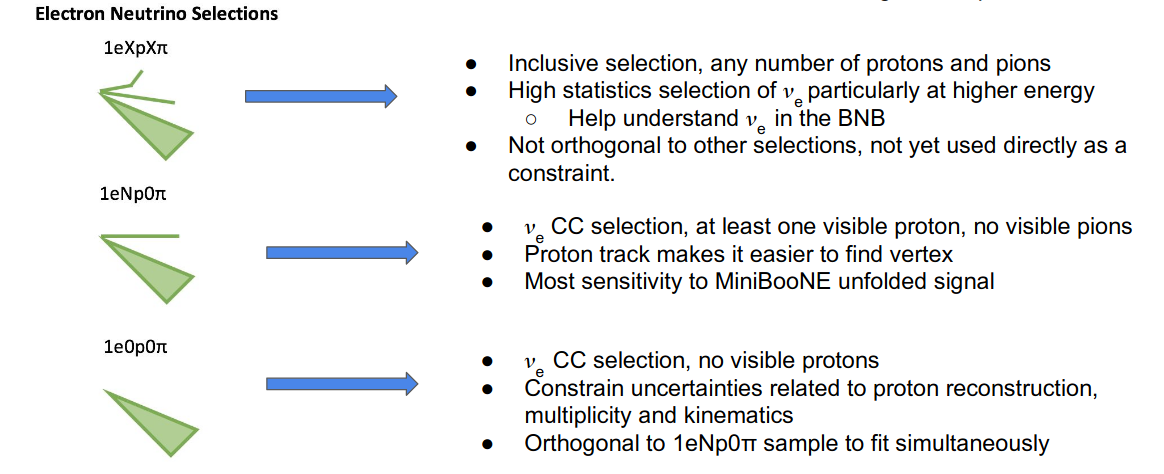
\includegraphics[width=0.85\textwidth]{introduction/nueselections.png}
%\caption{\label{fig:nueselections}Schematic of the three $\nu_e$ selection in this analysis, outlining the goals and strengths of each. In this work, the threshold for a visible proton at truth-level proton is 40 MeV of KE. $N$ refers to one or more and $X$ to any number of final state particles of a given category.}
%\end{center}
%\end{figure}


\begin{table}[ht]
\caption{\label{tab:selectionsNue} Schematic of the three $\nu_e$ selections, outlining the definition and goals of each. In this work, the threshold for a visible proton at truth-level proton is 40 MeV of KE. N refers to one or more and X to any number of final state particles of a given category.}
\centering
\begin{tabular}{ m{0.1\textwidth} | m{0.2\textwidth}  m{0.45\textwidth}  }
Channel & Description & Goal \\
\hline
 \begin{center}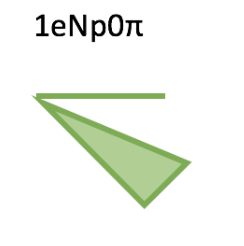
\includegraphics[width=0.1\textwidth]{introduction/1eNp}\end{center}& At least one visible proton and no visible pions & Most sensitive channel to MiniBooNE unfolded signal. The presence of a proton facilitates vertex finding.\\
\hline
 \begin{center}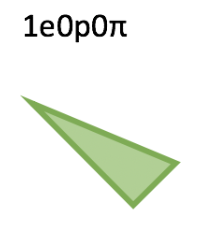
\includegraphics[width=0.1\textwidth]{introduction/1e0p}\end{center}& No visible protons and no visible pions & Constrain uncertainty related to proton reconstruction, multiplicity and kinematics for the 1$e$N$p$0$\pi$ channel.\\
\hline
\begin{center}\includegraphics[width=0.1\textwidth]{introduction/inclusive} \end{center} & Inclusive Selection: any number of protons and pions & Helpful to understand $\nu_e$ in the BNB: high statistic selection, especially at higher energies ($>$ 700 MeV). Not used as a constraint for other channels. \\
\hline
\end{tabular}
\label{tab:gt}
\end{table}


\par %\textbf{agnostic selection} 
In devising the selections presented above, we have deliberately chosen to not rely on cuts that make use of kinematic features of low-energy $\nu_e$ events. This allows the analysis to be agnostic to possible sources of new physics, and limits model dependence associated with assumptions on intrinsic $\nu_e$ interaction kinematics. Furthermore, an agnostic selection strategy allows to explore the kinematics of $\nu_e$ candidate events after their selection, for a full investigation of the origin of a potential anomaly. Implementing this choice requires the ability to fully leverage the information provided by the MicroBooNE LArTPC for $\nu_{\mu}-\nu_e$ and $e-\gamma$ separation. Significant progress has been made in developing tools for this goal, and will be described in subsequent sections. 




\subsection{Signal Model \textcolor{green}{David  ... (P.R. Elena) }}
\begin{comment}
%%%%%%% these are various parts that have been moved/modified
In order to benchmark the performance of the analysis it is valuable to have a signal model which can be used to assess the analysis' sensitivity.  This section describes the choice of model used for this purpose. It is important to stress that the signal model used serves the purpose of benchmarking the analysis' sensitivity, but the ultimate goal of our analysis remains to measure the rate of $\nu_e$ interactions in the BNB and report whether the observation is consistent or not with MicroBooNE's MC prediction.

\par Ultimately many signal models can be produced to test an analysis' sensitivity, each with its own set of important assumptions and caveats. % Or...
Ultimately any signal model used to test the analysis' sensitivity will carry a set of important assumptions and caveats. 
While reporting sensitivities for the MB-$\nu_e$ LEE model is useful, it is not exhaustive in being able to address MicroBooNE's ability to address MiniBooNE's anomaly. 
\end{comment}


\par  Many models can be devised to explain the MiniBooNE LEE as an excess of $\nu_e$ interactions, each model relying on a given (new) physics production mechanism and set of assumptions on the detector response. This section describes the signal model chosen by the collaboration to benchmark the sensitivity of all $\nu_e$ LEE analyses, including ours.  While a signal model is a useful tool, it is important to stress that any signal model carries a set of important assumptions and caveats, and that the ultimate goal of our analysis remains to measure the rate of $\nu_e$ interactions in the BNB, reporting whether the observation is consistent or not with MicroBooNE's MC prediction. Answering whether MicroBooNE's observation is consistent with the MiniBooNE LEE anomaly is beyond the scope of this work, and something not achievable without significant work for both MiniBooNE and MicroBooNE.
\begin{comment}
\par To test this analysis' sensitivity, a model explaining the MiniBooNE LEE  as an excess of $\nu_e$ interactions must be produced and used to generate simulated events in MicroBooNE. Many such models can be devised, each relying on a given (new) physics production mechanism and set of assumptions on detector response. 
\end{comment}

\par  The signal model used to generate simulated events in MicroBooNE and to compute the primary sensitivity quoted by this analysis  is the MiniBooNE-unfolded LEE model, referred to as \textbf{MB-$\nu_e$ LEE} model \cite{C,C2}. In this model, all excess LEE events are assumed to be due to $\nu_e$ interactions with a value of true energy obtained by unfolding from the reconstructed CCQE energy of MiniBooNE LEE events, as recorded by MiniBooNE's data. This procedure is performed by relying on MiniBooNE's energy smearing matrix. The resulting true neutrino energy distribution is shown in figure~\ref{fig:minibooneunfolded}. There are several limitations to this model worth observing, some technical, others conceptual. On a technical level, the model is composed of a binned event distribution, rather then a parametrized or analytic prediction of the expected $\nu_e$ spectrum. Additionally, no events below 200 MeV of true energy exist in this model. 
\begin{figure}[ht]
\begin{center}
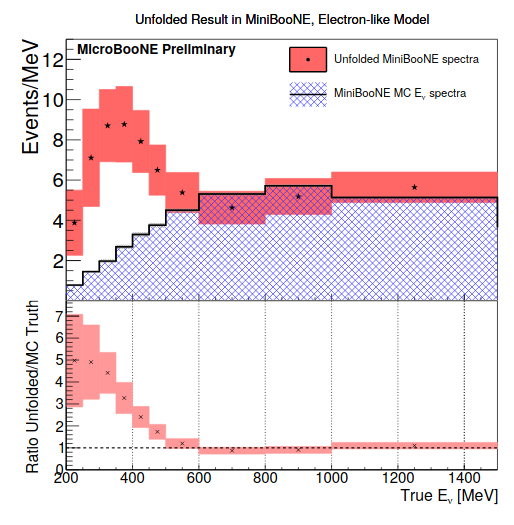
\includegraphics[width=0.45\textwidth]{introduction/unfoldedminiboone.png}
\caption{\label{fig:minibooneunfolded}MB-$\nu_e$ LEE signal model extracted from MiniBooNE's results.}
\end{center}
\end{figure}
Conceptual issues can be raised in association with the various assumptions made to generate the model. These include the strong reliance on MiniBooNE's simulation in order to unfold reconstructed to true neutrino energy, and the choice of such an unfolding procedure (performed as a function of $E_{\rm CCQE}$ rather then EM energy and $\theta$, for example).
It is especially important to note that the chosen model strongly favors the interpretation of MiniBooNE events as originating from very low energies (200-400 MeV) for which achieving high sensitivity may come at the cost of omitting a robust analysis at higher energies. This is something the analysis tries to avoid by developing an inclusive and kinematically unbiased analysis workflow. At the same time, we explore additional models for sensitivity calculations, most notably a 3+1 sterile-neutrino oscillation model. This is discussed in more detail in section~\ref{sec:Sensitivity2Osc}.
\par Figure~\ref{fig:nuerate} shows the expected $\nu_e$ rate as a function of true neutrino energy split by final-state topology for the available MicroBooNE dataset of $10.1E20$ POT. % with a 10 cm FV. 
 MB-$\nu_e$ LEE signal events are shown in orange.
\begin{figure}[H] 
\begin{center}
    \begin{subfigure}[b]{0.45\textwidth}
    \centering
    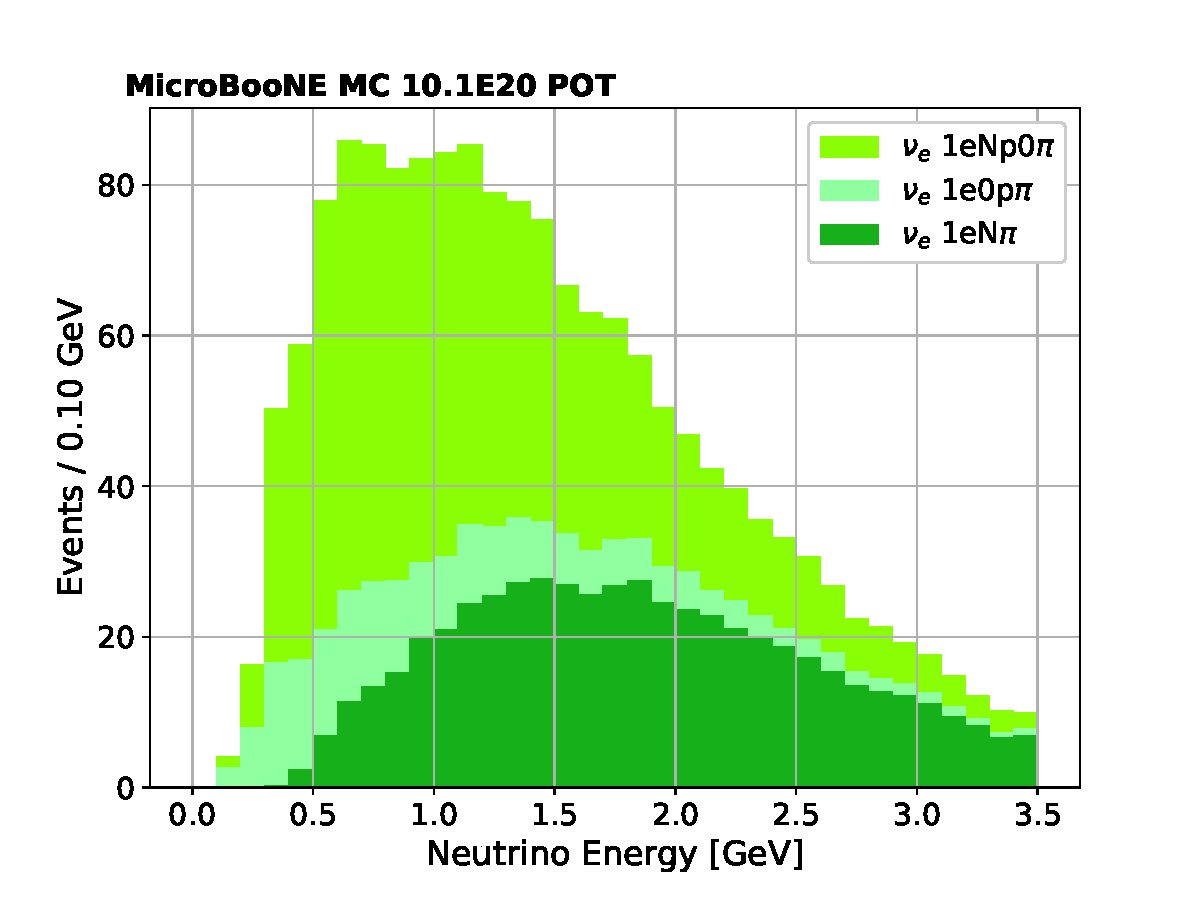
\includegraphics[width=1.00\textwidth]{introduction/nue_rate_MCC9.pdf}
    %\caption{\label{fig:nuerate:prediction}}
    \end{subfigure}
    \begin{subfigure}[b]{0.45\textwidth}
    \centering
    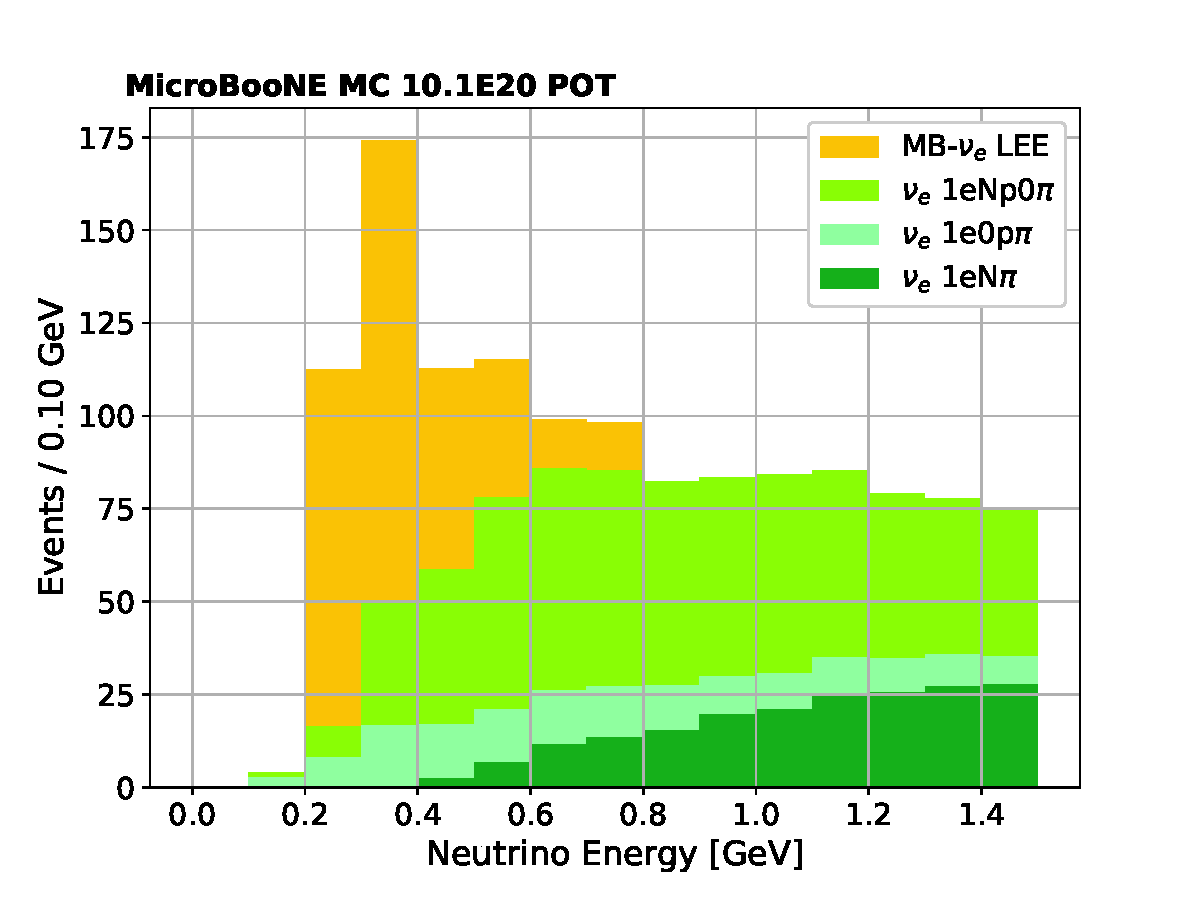
\includegraphics[width=1.00\textwidth]{introduction/nue_rate_MCC9_LEE.pdf}
    %\caption{\label{fig:nuerate:prediction:MC}}
    \end{subfigure}
\caption{\label{fig:nuerate}Expected $\nu_e$ rate in MicroBooNE for $10.1E20$ POT %in a 10-cm FV 
 subdivided by event topology (1$e$N$\pi$,1$e$N$p$0$\pi$, and 1$e$N$p$0$\pi$). The right-hand side figure highlights the low energy region with the unfolded $MB-\nu_e$ LEE signal prediction in orange.}
\end{center}
\end{figure}

\subsection{Goals of the $\nu_{\mu}$ Selection \textcolor{green}{David   ... (P.R. Elena)}}
\label{ssec:goalsofnumusel}
\begin{comment}
\par For the purpose of this analysis, measurements of $\nu_{\mu}$ interactions are aimed at reducing modeling uncertainties for intrinsic $\nu_e$ events and backgrounds, with the goal of reducing systematic uncertainties in order to be able to claim the observation of new physics were a measurement of $\nu_e$ interactions differ significantly from the expected intrinsic rate. This section describes why such a data-driven constraint is needed and what are the choices which motivate the approach taken in this analysis.
\end{comment}
\par In the context of this analysis, measurements of $\nu_{\mu}$ interactions are aimed at reducing modeling uncertainties for intrinsic $\nu_e$ events and backgrounds. Event reconstruction and $\nu_e$ identification are only one of the challenges in this analysis:  in order to make statements on whether the observed $\nu_e$ rate indicates the presence of new physics, a well understood prediction of the intrinsic $\nu_e$ rate is needed. 

\par Uncertainties in the expected $\nu_e$ rate are associated to reconstruction efficiencies (detector effects) as well as modeling uncertainties in both the $\nu_e$ flux  and neutrino-argon cross-section predictions. Here, we focus on describing the strategy to deal with the latter. In the case of a single detector experiment, %uncertainties in the intrinsic $\nu_e$ interaction rate are rather large:  and can limit the ability to associate a $\nu_e$ measurement with potential new physics if not a constraint through additional measurements is needed. 
flux uncertainties for $\nu_e$ calculated from the beam simulation are $\mathcal{O}$(10\%) above 800 MeV and grow to 40\% at 200 MeV;  cross-section uncertainties are also large, due to the scarcity of $\nu$-Ar cross-sections measurements -- especially at low energy -- and due to the complex modeling of neutrino interactions on heavy targets such as argon. Combining all effects, the uncertainty on the $\nu_e$ interaction rate in the few-hundred MeV energy range in MicroBooNE could be as high as 100\%.
\par To reduce modeling uncertainties on the expected rate of $\nu_e$ interactions, data-driven constraints are required. These can be performed through measurements of $\nu_{\mu}$ interactions impacted by the same underlying modeling uncertainties. In order to constrain flux uncertainties, we rely on the fact that $\nu_e$ and $\nu_{\mu}$ intrinsic to the beam are produced by the decay of the same parent $\pi$ and $K$ flux. Similarly, we rely on the charged-current interaction mode $\nu_{l} + Ar \rightarrow l + X$ common to both $\nu_{\mu}$ and $\nu_e$ interactions to constrain the uncertainties on the $\nu_e$ interaction modeling.


\begin{comment}

The complexity of $\nu$-Ar interactions and of hadronic interactions in the beamline mean that many different handles and measurements of $\nu_{\mu}$ interactions can play a role in constraining different uncertainties. As examples, measurement of CC and NC $\pi^0$ production constrain resonant interactions and thus $\pi^0$ backgrounds to the $\nu_e$ selection, and measurements of high-energy $\nu_{\mu}$ interactions can help constrain the kaon flux in the beam, which contributes substantially to the production of intrinsic $\nu_e$s. Likewise, measurements of low-energy $\nu_{\mu}$s can help constrain poorly understood $\nu$-Ar interaction models in the few-hundred MeV energy regime, a critical requirement for this analysis. The neutrino identification work developed for this analysis, referred to as \texttt{SliceID} and described in section~\ref{sec:sliceID}, is a highly efficient and topology agnostic selection that enables a vast program of $\nu_{\mu}$ measurements, allowing for flexibility in selecting topologies that may have the strongest constraining power and thus most benefit the $\nu_e$ analysis. At the current time, as described in the remainder of this section and in section~\ref{sec:systematics}, the emphasis is on the measurement of low-energy $\nu_{\mu}$ interactions with the goal of constraining the large uncertainties in low-energy $\nu_e$ events which significantly impact the analysis.
\par To further motivate the need for low energy $\nu_{\mu}$ interactions, we describe two important ways in which such a dataset can benefit the reduction of modeling uncertainties for $\nu_e$ interactions.
\end{comment}
\par The richness of $\nu$-Ar interactions and of hadronic interactions in the beamline offers a number of different handles 
to constraint different uncertainties via the measurements of $\nu_{\mu}$ interactions.
As examples, measurements of CC and NC $\pi^0$ production can be used to constrain resonant interactions and thus $\pi^0$ backgrounds to the $\nu_e$ selection;  measurements of high-energy $\nu_{\mu}$ interactions can help constrain the kaon flux in the beam, which contributes substantially to the production of intrinsic $\nu_e$s. Likewise, measurements of low-energy $\nu_{\mu}$s can help constrain poorly understood $\nu$-Ar interaction models in the few-hundred MeV energy regime, a critical requirement for this analysis.  At the current time, we focus our effort on the study with the bigger impact to the analysis: we perform the measurement of low-energy $\nu_{\mu}$ interactions with the goal of constraining the large uncertainties in low-energy $\nu_e$. A detailed  description of this constraint is shown in the remainder of this section and in section~\ref{sec:systematics}.
%At the current time, our effort is focused on the measurement of low-energy $\nu_{\mu}$ interactions with the goal of constraining the large uncertainties in low-energy $\nu_e$ events which significantly impact the analysis; a detailed  description of this constraint is shown in the remainder of this section and in section~\ref{sec:systematics}.
 However, it should be noted that the neutrino identification work described in section~\ref{sec:sliceID} results in a highly efficient and topology agnostic selection: such a flexible selection allows for a number of $\nu_{\mu}$ measurements and their associated constraints to be implemented in case the $\nu_e$ analysis needs a stronger constraining power. 



\par To further motivate the need to study low energy $\nu_{\mu}$ interactions, we describe two important ways in which such a dataset can lead to a reduction of modeling uncertainties for $\nu_e$ interactions. Figure~\ref{fig:numuconstraint:flux} shows the flux correlation for $\nu_{\mu}$ (bottom left) and $\nu_e$ (top right) interactions obtained from MicroBooNE's adaptation of the BNB flux simulation developed by MiniBooNE~\cite{bib:fluxmcc9,bib:fluxtechnote}. Red (blue) areas show large (anti-)correlation. The top-left or bottom-right quadrants show the strength of correlations between the two flavors. For $\nu_e$ energies below 1 GeV, correlations are strongest with $\nu_{\mu}$ interactions at low energy \textcolor{blue}{should we add some more details on the assumptions behind this correlation matrix? or on how this correlation matrix is calculated (is it simply from the beam MC?) Elena}. Figure~\ref{fig:numuconstraint:xsec} shows different cross-section predictions for $\nu_{\mu}$ and $\nu_e$ interactions. The dashed and solid curves represent the CCQE cross-section used in MCC8 vs. MCC9 respectively. Below 400 MeV, the difference in event rates for different models is larger then 100\%. The large differences between these curves, particularly at low energy, indicate the strong need to constrain cross-section uncertainties with MicroBooNE's own data. 
\begin{figure}[ht] 
\begin{center}
    \begin{subfigure}[b]{0.42\textwidth}
    \centering
    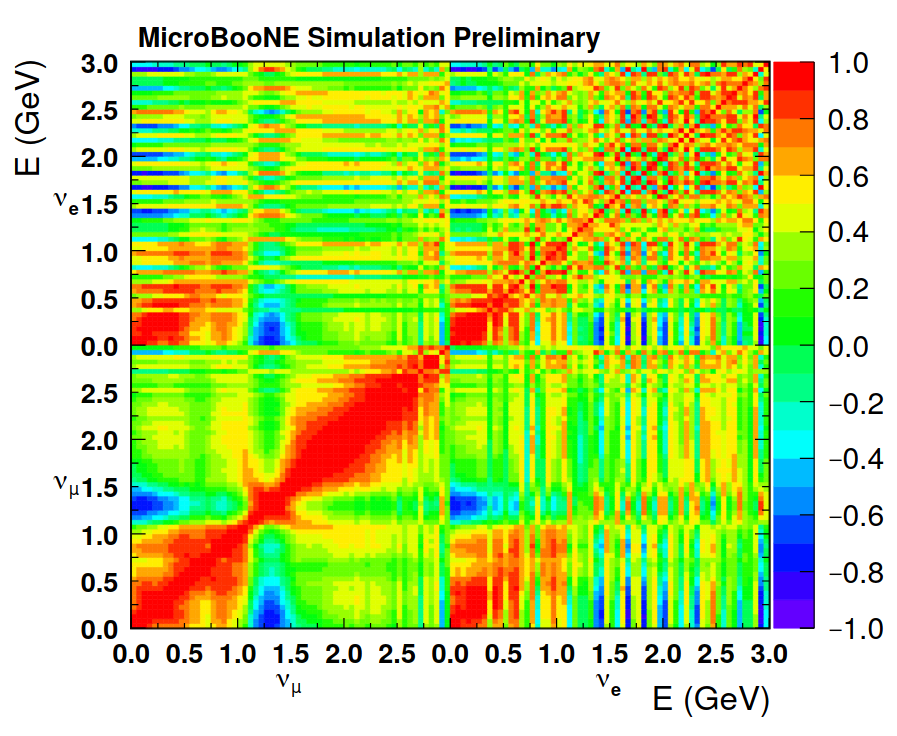
\includegraphics[width=1.00\textwidth]{introduction/fluxcorrelation.png}
    \caption{\label{fig:numuconstraint:flux}}
    \end{subfigure}
    \begin{subfigure}[b]{0.3\textwidth}
    \centering
    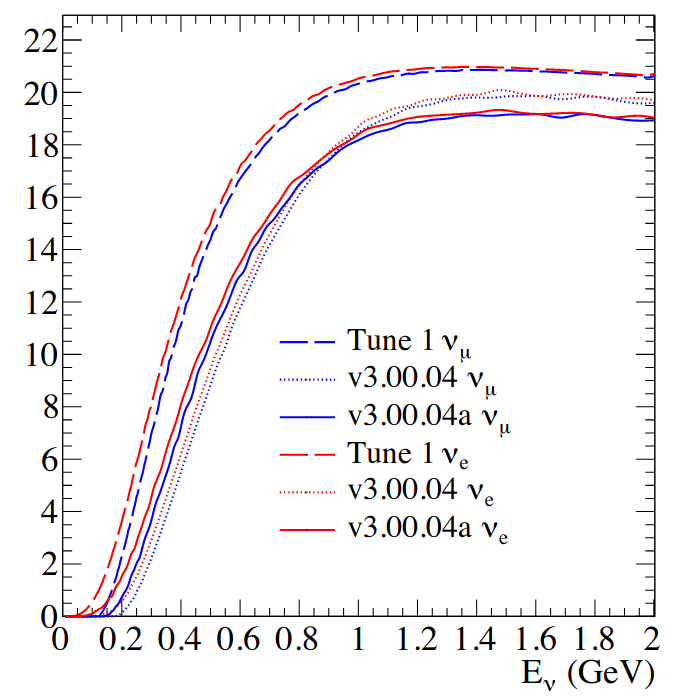
\includegraphics[width=1.00\textwidth]{introduction/xsec_mcc8_mcc9.png}
    \caption{\label{fig:numuconstraint:xsec}}
    \end{subfigure}
\caption{\label{fig:numuconstraint} (a) $\nu_{\mu}$-$\nu_e$flux correlation matrix. (b) Different cross section models for CC interactions \textcolor{blue}{Y axis label is missing}.  }
\end{center}
\end{figure}

\subsection{Systematics \textcolor{green}{David... (P.R. Elena)}}
\par This section gives a brief overview of how detector and modeling uncertainties are accounted for in the analysis. The estimation of systematics is performed in section~\ref{sec:systematics}.
\par \noindent \textbf{Detector Systematics}: Detector modeling in MicroBooNE has undergone significant updates in the past year, in part as a result of the large impact that detector systematics have had on 2018 analyses \cite{bib:CCpi0, bib:CCincl}. Detector effects with significant impact on the analysis can be broken up into three main categories:
\begin{itemize}
    \item[-] Wire-Response modeling: the response of MicroBooNE's electronics to drifting charge is a complex subject described in three past publications~\cite{bib:noise,bib:SP1,bib:SP2}. The work of these papers in improving the understanding and modeling of noise and field-response effects has been implemented in the current detector simulation and is expected to lead to a reduction in what for MCC8 analysis comprised the largest detector uncertainty.
    \item[-] Space-Charge modeling: MicroBooNE's space-charge model has changed significantly since 2018, moving from a calculation-based~\cite{bib:SCEsim} implementation of electric field distortions to a data-driven E-field map~\cite{bib:SCEdata} implemented in simulation and reconstruction. Due to the large position distortions (and, though smaller, charge distortions) SCE can significantly impact an analysis through the determination  of fiducial boundaries, tracking and energy resolution.
    \item[-] Scintillation light modeling: MicroBooNE's model of scintillation light production has not changed significantly since the beginning of data-taking, and has known limitations. Of particular importance to this analysis, which aims to use a dataset spanning four years, is the known and significant time-dependent variation of MicroBooNE's light response. This analysis takes several steps to correct for, and mitigate the impact of light mismodeling. Triggering on low-energy signal $\nu_e$ events, and cosmic-rejection are particularly sensitive to scintillation light detector effects.
\end{itemize}
\emph{An additional detector effects that needs to be accounted for is ion Recombination which impacts the detector's calorimetric response. Tailored studies and proton samples are being developed to assess ion recombination modeling accuracy in MCC9 but are not available at the time of writing of this note.}
\par \noindent \textbf{Flux and Cross-Section Modeling} Uncertainties in flux and cross-section modeling are treated through a \emph{multi-sim} approach, where underlying parameters that are input to the modeling are varied in a correlated way. Flux uncertainties are taken from the MiniBooNE BNB flux simulation adapted to MicroBooNE~\cite{bib:fluxmcc9,bib:fluxtechnote}, while $\nu$ interaction uncertainties are handled within the \texttt{GENIE} reweighting package, as described in~\cite{bib:geniesupportnote}. \emph{We note that the \texttt{GENIE} event reweighting infrastructure is still in development and likely to be updated or further expanded on in the future. Finally, uncertainties associated with pion and proton re-interactions in argon were unavailable when this version of the Tech Note was produced and not included at this stage.} 

\subsection{Sensitivity Estimation \textcolor{green}{Nico/Maya... (P.R Elena)}}
In order to extract information from the selected events, a simple hypothesis test is performed.
Given an observable quantity, such as a measurement of the energy deposited by the neutrino interaction, the hypothesis in which the observed spectrum of events is entirely due to the standard model, $H_0$, is tested against an alternative hypothesis $H_1$.
The alternative hypothesis $H_1$ consists of all the known background plus the LEE unfolded signal from MiniBooNE (MB-$\nu_e$ LEE), though an oscillation signal has also been studied, as shown in section \ref{sec:Sensitivity2Osc}.
For the MB-$\nu_e$ LEE signal, the hypothesis test is simple in that the comparison of two different hypotheses is performed and no parameter is inferred from the data.

%The hypothesis test is simple in the sense no parameter is fitted from the data, but we limit ourselves to a comparison of two different hypotheses.

A test statistic is chosen in order to condensate all information of the observables in one number.
Through toy experiments, the expected distributions of the test statistic under the two hypotheses is calculated; the separation power is computed by taking the median p-value with respect to $H_0$ under the assumption that %one might observe if 
 $H_1$ is true. This is the discovery sensitivity, i.e. the sensitivity to reject $H_0$ when $H_1$ is true.
We studied the sensitivity in different cases. First, we describe in detail the sensitivity calculation considering only statistical uncertainties. Given that only a handful of events pass the exclusive selections, the impact of statistical uncertainties plays a large role in determining the analysis' ultimate sensitivity. We also include systematic uncertainties using the covariance matrix formalism and the SBNfit package, as described in section \ref{subsec:sensitivity_syst_uncertainty}.
Finally, the observed spectra from the \nueccnopinp and the \numu selections are analyzed simultaneously using a single covariance matrix to constraint the systematic uncertainties and thus increase the sensitivity.

\subsection{Analysis Status \textcolor{red}{Elena/David/ Group discussion}}

\par The work presented in this note has matured into a robust and comprehensive analysis, with strong tools which are able to leverage the calorimetric and topological imaging of the LArTPC technology to identify in a kinematically agnostic selection $\nu_e$ interactions in MicroBooNE's BNB dataset. The analysis, as it stands, is able to make interesting conclusions on the $\nu_e$ content of the BNB flux, with the primary limitation to the power of these conclusions driven by the low selection efficiency at low energy .
\par Multiple selections have been developed as part of this analysis, all showing generally good data-simulation agreement, as shown in figure~\ref{fig:datamccomparisons} for the \npsel pre-selection (figure~\ref{fig:datamccomparisons:nuepresel}, Run 1) and for the full $\nu_{\mu}$ contained selection (figure~\ref{fig:datamccomparisons:numu}, Run 3).

\begin{figure}[ht] 
\begin{center}
    \begin{subfigure}[b]{0.4\textwidth}
    \centering
    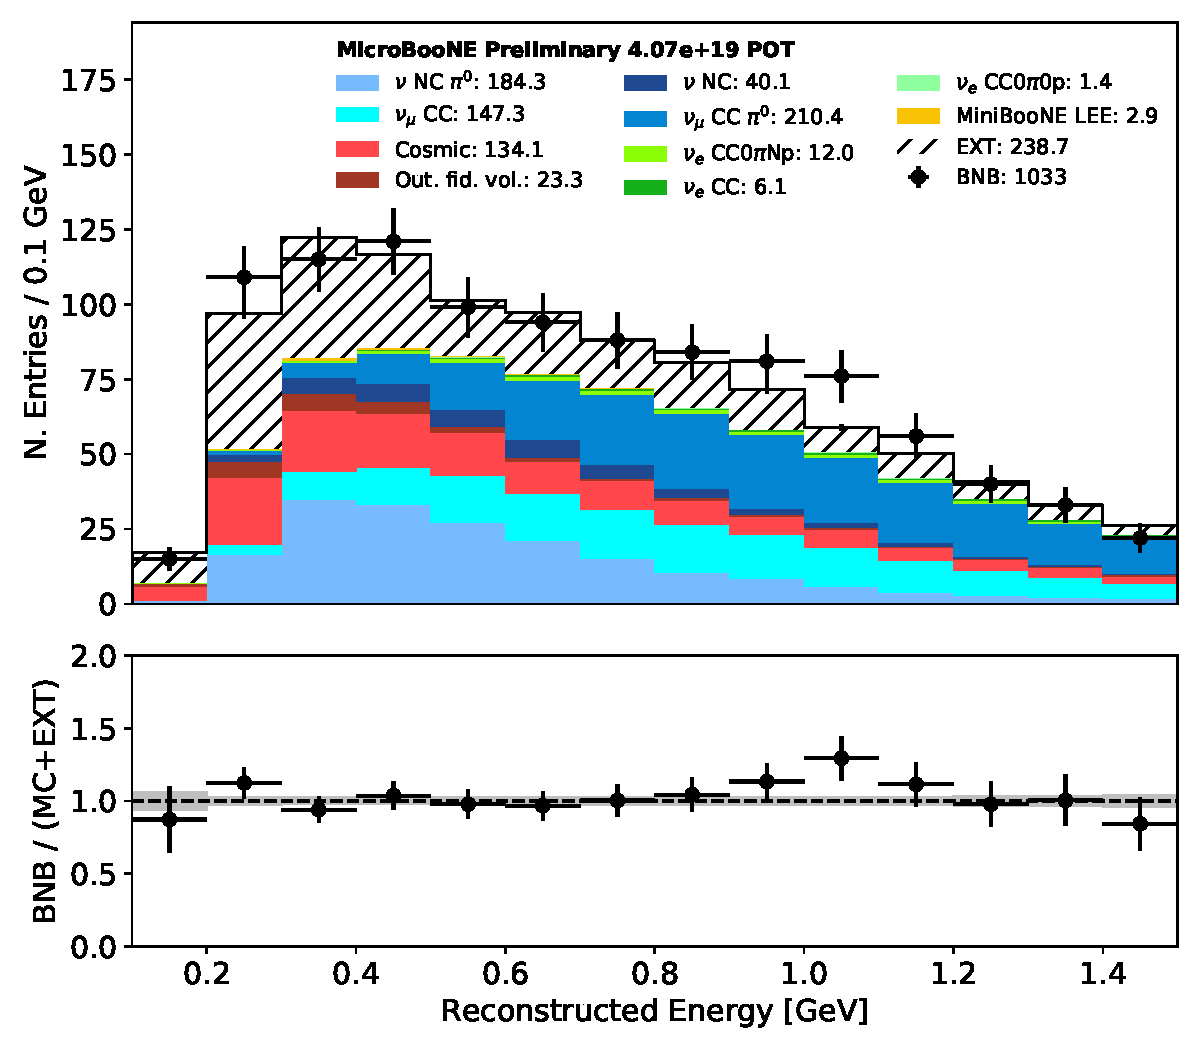
\includegraphics[width=1.00\textwidth]{1eNp/reco_e_01162020_RUN1.pdf}
    \caption{\label{fig:datamccomparisons:nuepresel} \npsel pre-selection for Run  1}
    \end{subfigure}
    \begin{subfigure}[b]{0.44\textwidth}
    \centering
    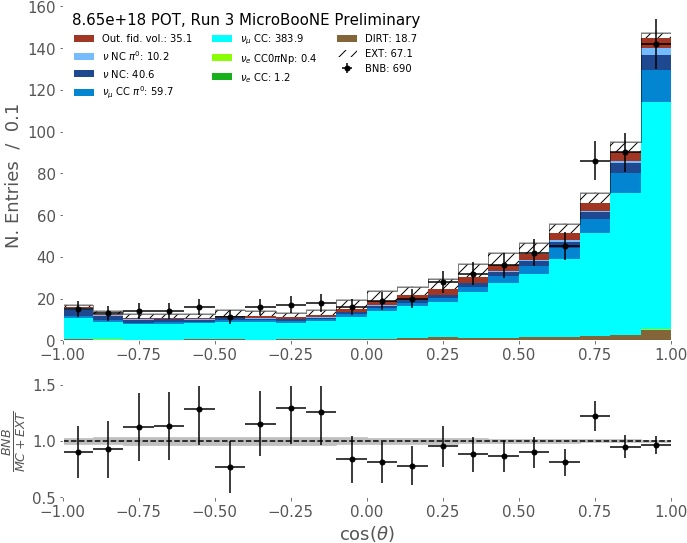
\includegraphics[width=1.00\textwidth]{NuMuCCsel/Images/Ryan/Run3_costheta_withCRT.jpg}
    \caption{\label{fig:datamccomparisons:numu} high-purity $\nu_{\mu}$ for Run 3}
    \end{subfigure}
\caption{\label{fig:datamccomparisons} }
\end{center}
\end{figure}

\par The three $\nu_e$ selections developed in this work all provide strong input to the analysis. Figure~\ref{fig:intro:nueselections} shows the status of the box-cut \npsel (figure~\ref{fig:intro:nueselections:1eNp}), the BDT-based (figure~\ref{fig:intro:nueselections:1e0p}), and the BDT-based $\nu_e$ inclusive (figure~\ref{fig:intro:nueselections:inclusive}). \par The inclusive channel provides the analysis a tool with which to study the modeling of $\nu_e$ interactions, especially at higher energies, and provides a first validation even with the small dataset currently available. Moving forward, we are exploring ways to use this channel to quantitatively constrain high-energy $\nu_e$ modeling uncertainties.
\par The 1$e$0$p$0$\pi$ channel obtains a purity of 49\% and, even though it currently primarily is sensitive to higher-energy $\nu_e$ interactions, provides a valuable validation of detector and modeling effects which can cause migration from the N$p$ to 0$p$ channel. A quantitative estimation of the impact of this channel is being performed.
\par The \npsel channel, in the box-cut selection, achieves a $5-10$\% efficiency with a 73\%  purity for the cut-based  and a $5-15$\% efficiency with a 81\%  purity for the BDT-based selection. These selections lead to $\mathcal{O}$(10) expected MB-$\nu_e$ LEE signal events and $40-70$ intrinsic $\nu_e$ events for the full Run $1-4$ dataset. The final reconstructed energy distribution for the box-cut selection is shown in figure~\ref{fig:intro:nueselections:1eNp}. The box-cut selection's statistics-only sensitivity is $2.1-2.3\sigma$, depending on the test-statistic used. The low statistics of the predicted signals lead to significant fluctuations in the expected sensitivity, covering the range $1.5-3.1\sigma$. 
 \emph{Given the efficiency and purity obtained with the BDT-based workflow, we expect a higher sensitivity compared to the cut-based workflow.  We are in the process of re-evaluating the BDT-based performance which will be reported in this note after higher statistics MC samples have been included, and a re-calibration of the calorimetry has been completed.} 

\begin{figure}[ht] 
\begin{center}
    \begin{subfigure}[b]{0.28\textwidth}
    \centering
    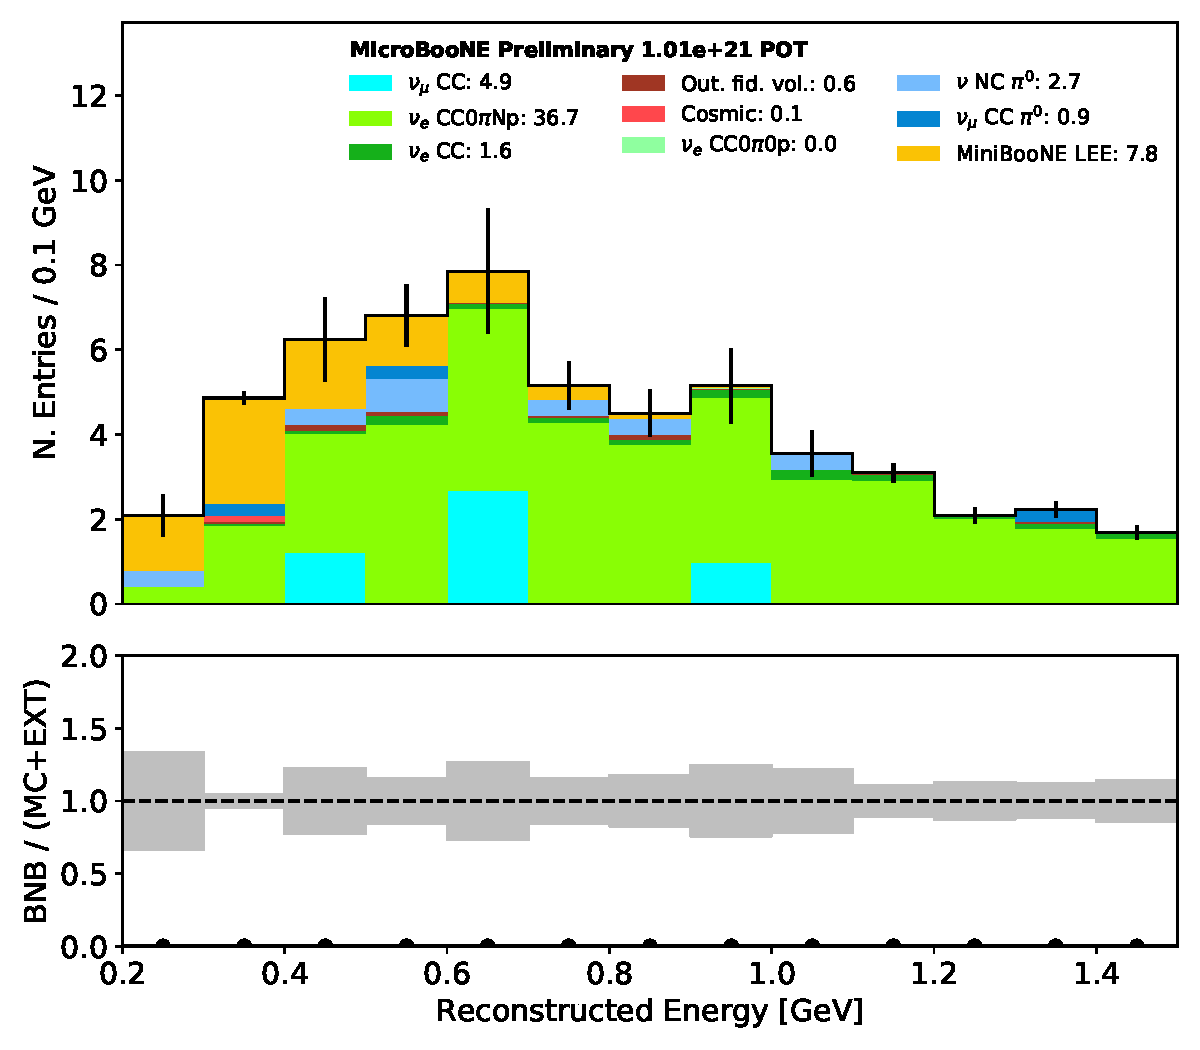
\includegraphics[width=1.00\textwidth]{1eNp/reco_e_01162020_box_RUN1.pdf}
    \caption{\label{fig:intro:nueselections:1eNp} box-cut $\nu_e$ 1$e$0$p$}
    \end{subfigure}
    \begin{subfigure}[b]{0.28\textwidth}
    \centering
    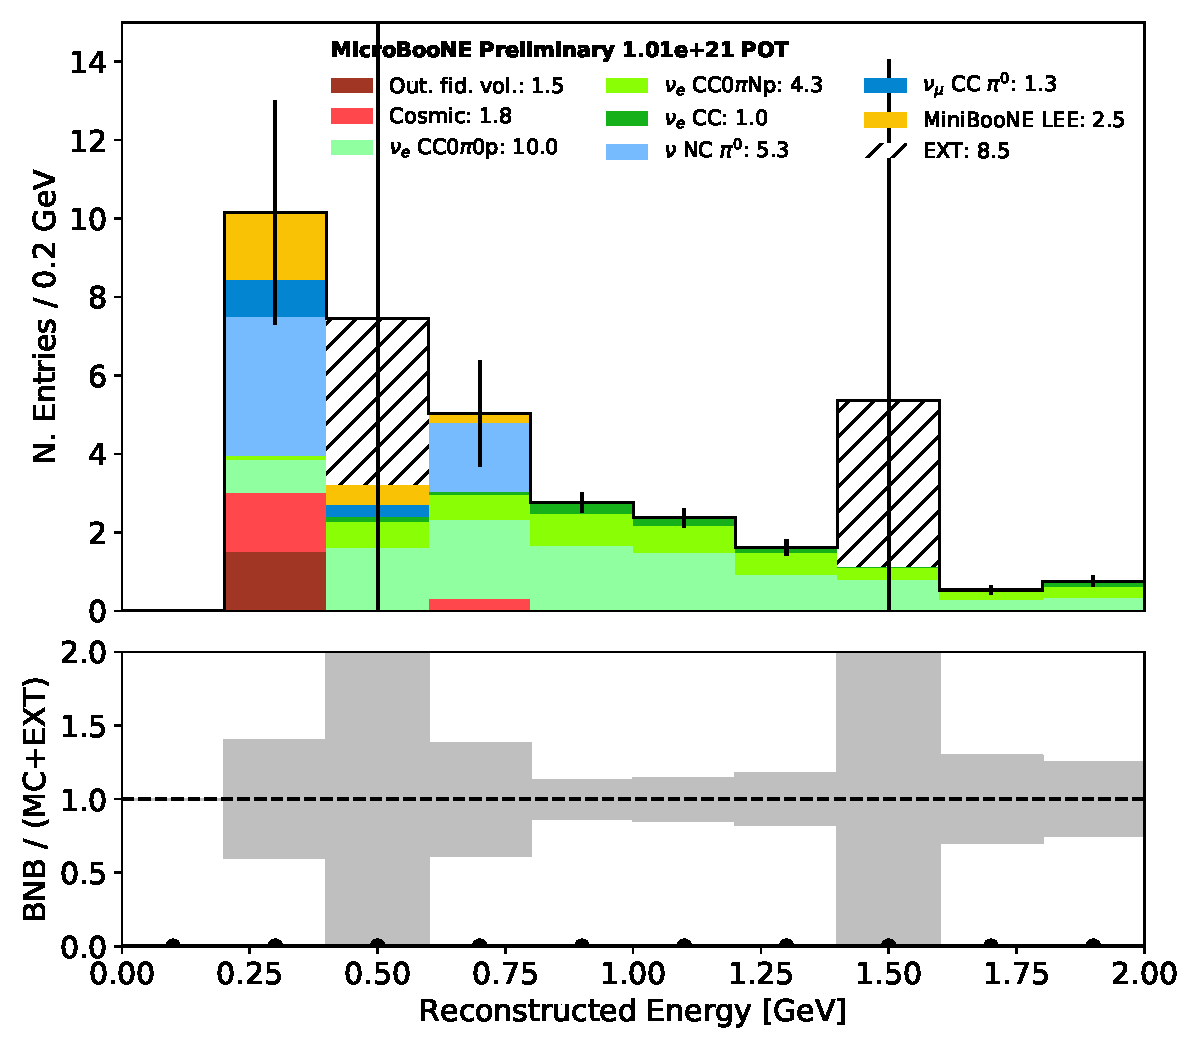
\includegraphics[width=1.00\textwidth]{1e0p/reco_e_01162020_RUN3_bgbdt.pdf}
    \caption{\label{fig:intro:nueselections:1e0p} bdt-based $\nu_e$ 1$e$0$p$}
    \end{subfigure}
    \begin{subfigure}[b]{0.31\textwidth}
    \centering
    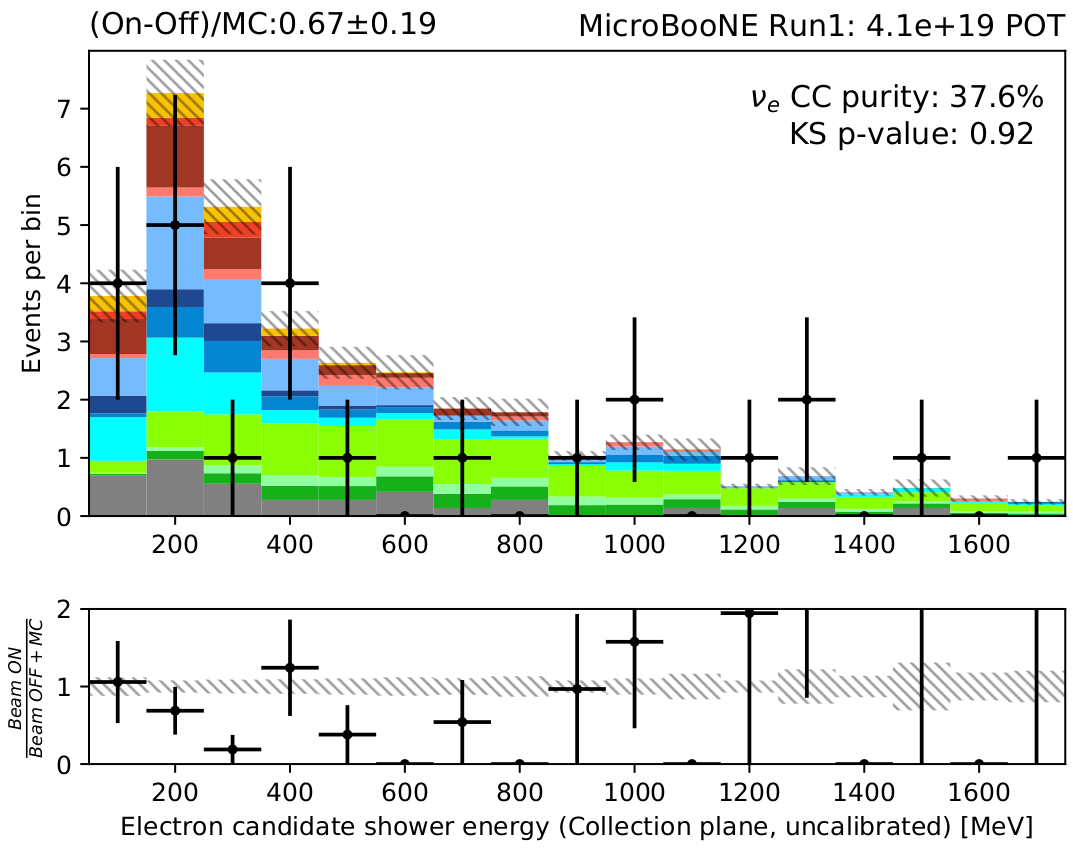
\includegraphics[width=1.00\textwidth]{introduction/nueinclusive.png}
    \caption{\label{fig:intro:nueselections:inclusive} BDT-based $\nu_e$ inclusive}
    \end{subfigure}
\caption{\label{fig:intro:nueselections} }
\end{center}
\end{figure}


\par A particular strength of this analysis consists in the multiple sideband channels available to validate the simulation, reconstruction, and help constrain $\nu_e$ interaction uncertainties. A high statistics $\pi^0$ sideband (section~\ref{sec:controls:pi0}) provides confidence in the performance of the analysis' shower reconstruction. A high-quality inclusive contained $\nu_{\mu}$ selection shows good data-simulation agreement in both Run 1 and Run 3 and provides the input for the $\nu_{\mu}$ constraint which has the primary goal of reducing systematic uncertainties for low-energy $\nu_e$s. A primary estimation of the impact of the $\nu_{\mu}$ constraint shows a 50\% reduction in modeling uncertainties, though this is to be revisited by the time of the February collaboration meeting. Additionally, an inclusive $\nu_{\mu}$ selection (section~\ref{sec:nueselection:inclusive}) provides a valuable starting point for many possible final-state measurements which may become necessary to further validate the analysis as its review progresses. 
\par The full evaluation of systematics for this analysis has not yet been completed. Detector systematic samples available have been investigated and preliminarily show little impact on the selections (sec.~\ref{sec:systematics}) but have not yet been included in sensitivity calculations. The recent availability of an updated central-value simulation for \texttt{GENIE}, together with updated genie modeling uncertainties, will allow us to quantitatively measure the impact of these uncertainties, with and without sideband channel constraints, by the February collaboration meeting. In the meantime, sections~\ref{sec:systematics} and~\ref{sec:sensitivity} present the status of tools and methods used for the full evaluation of the analysis' sensitivity. Statistics-only sensitivity calculations are also presented, based on the box-cut \npsel described in this note.


\newpage

\newpage

\section{Overview of Neutrino Identification}
\label{sec:sliceID}
%\subsection{Event Slicing and Cosmic Removal in Pandora}
The work presented in this note relies on the Pandora event reconstruction~\cite{bib:pandoraub}. Pandora does the low-level pattern-recognition step of the reconstruction, i.e. groups hits into clusters, clusters into particles and particles into hierarchies. This section focuses on the cosmic rejection aspect of the analysis. We describe here how the output of Pandora's pattern-recognition is combined with scintillation light to isolate possible candidate neutrino interactions in MicroBooNE. This process is illustrated in the three images of Figure~\ref{fig:sliceid}. Moreover, we describe how the additional information from the Cosmic Ray Tagger (CRT) is used to improve cosmic rejection in the \numu selection. 

\begin{figure}[ht] 
\begin{center}
    \begin{subfigure}[b]{0.7\textwidth}
    \centering
    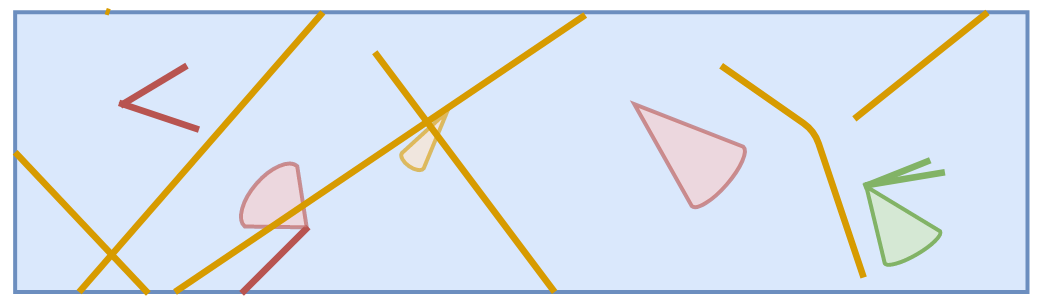
\includegraphics[width=1.00\textwidth]{NuId-Ch3/Images/slice00.png}
    \caption{\label{fig:slcieid:00} Typical event with multiple interactions isolated by Pandora in \texttt{slices}. Candidate neutrino interactions are shown in green and red.  Obvious cosmics are shown in orange.}
    \end{subfigure}
    \begin{subfigure}[b]{0.7\textwidth}
    \centering
    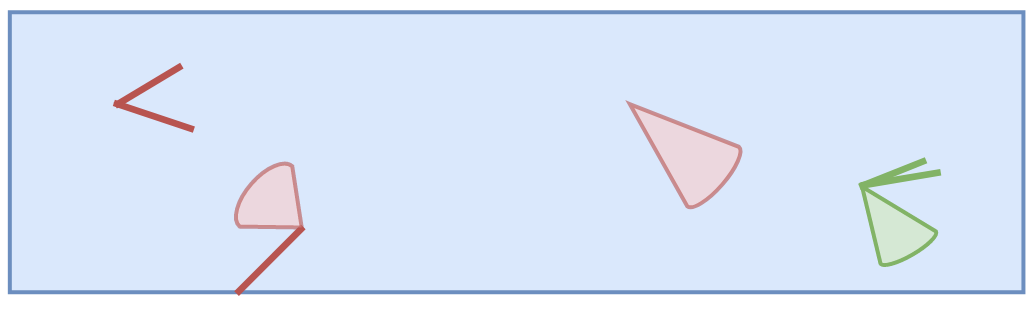
\includegraphics[width=1.00\textwidth]{NuId-Ch3/Images/slice01.png}
    \caption{\label{fig:slcieid:01} Event after the removal of \texttt{obvious cosmics} tagged geometrically by Pandora.}
    \end{subfigure}
    \begin{subfigure}[b]{0.7\textwidth}
    \centering
    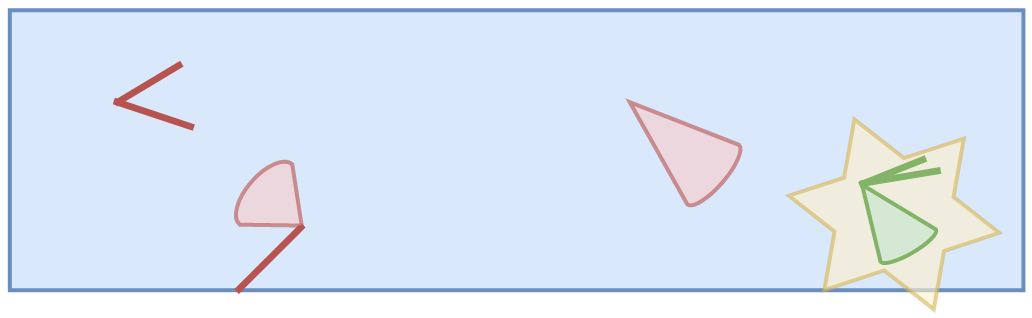
\includegraphics[width=1.00\textwidth]{NuId-Ch3/Images/slice02.png}
    \caption{\label{fig:slcieid:02} Implementation of the \texttt{SiceID} tool to isolate possible candidate $\nu$ interactions.  The selected candidate is highlighted, and shown in green.}
    \end{subfigure}
\caption{\label{fig:sliceid} Succession of steps in cosmic removal performed using Pandora's topological pattern recognition combined with scintillation light information through the \texttt{NeutrinoID} tool.}
\end{center}
\end{figure}

%\subsection{Slicing, Clustering and Vertexing}
\subsection{Pandora Slicing, Clustering and Vertexing}
The creation of a ``slice" is the first step of the Pandora processing. A slice is a collection of distinct reconstructed particles which belong to the same interaction, such as a cosmic muon and its Michel electron, or the muon and proton in a 1$\mu$1$p$ neutrino interaction. To produce slices, the Pandora cosmic pattern recognition is first run over all hits, aiming to construct muon tracks and any associated $\delta$-rays or Michel electrons under the cosmic hypothesis (fig.~\ref{fig:slcieid:00}). At this stage, obvious cosmic activity (through-going or out-of-time muons) is tagged using geometric information and discarded (fig.~\ref{fig:slcieid:01}). The remaining hit collection is used as input to Pandora and reconstructed both under the cosmic hypothesis and the neutrino hypothesis. A typical event contains approximately five slices at this stage. 

%\subsubsection{Clustering and Vertex Finding } 
\par In order to reconstruct the interactions in three dimensions, Pandora needs to match the information from at least two different views and create a neutrino vertex. Pandora performs the 2D clustering on the hits in each slice and on each plane separately. Then a number of 3D candidate vertices is created by finding positions that project down onto the ends of the available 2D clusters. All of the possible vertex candidates are fed into the support vector machine (SVM) vertex selection, and the candidate with the highest SVM score is chosen. This 3D vertex is used to split any existing clusters that cover the vertex. Then the cluster matching algorithms are run; in these algorithms the clusters are compared between views and modified to improve the matching.

\subsection{Pandora NeutrinoID: Cosmic Removal Via Topology and Scintillation Light}
\label{sec:sliceID:NeutrinoID}
\par After the set of Pandora pattern-recognition algorithms has isolated individual interactions into reconstructed slices and removed obvious cosmics, the remaining task is to identify which slice, if any, is associated with a neutrino interaction. Scintillation light information is used to reject slices incompatible with light recorded in-time with the beam. Topological cuts aimed at rejecting stopping-muon events which enter the TPC are also used. The \texttt{NeutrinoID} is at the core of all neutrino selections performed in this analysis; this first, common step is responsible for the majority of cosmic-rejection.
\\
\par We leverage three handles to distinguish between neutrino and cosmic-ray slices:
\begin{enumerate}
    \item Simple optical pre-selection cuts, which remove slices inconsistent with the beam flash;
    \item A topological score which assesses to what extent the slice looks like a neutrino interaction in the TPC (see DocDB 14175)
    \item A flash-matching score, which assesses how well the flash-hypothesis for the slice matches the beam flash.
\end{enumerate}

To select the neutrino slice, we first require a beam-triggered flash in the beam window. Then we apply the optical pre-selection cuts. If no slice passes optical pre-selection, the event is rejected. If the slice with the largest topological score passes the optical pre-selection, the slice forms the neutrino candidate; otherwise, the slice with the largest  flash-matching score forms the neutrino candidate. 
The performance of the \texttt{NeutrinoID} for simulated neutrino events is shown in~\cref{fig:sliceid_eff}.
Integrated over all final states and neutrino energies, the efficiency is:
\begin{itemize}
    \item[-] $\nu_\mu$ charged-current: \SI{83.0}{\%}
    \item[-] $\nu_e$ charged-current: \SI{83.3}{\%}
\end{itemize}
Further details on the \texttt{NeutrinoID} tool are available in DocDB 28418, 23854 and 22519.

\begin{figure}[H]
    \centering
    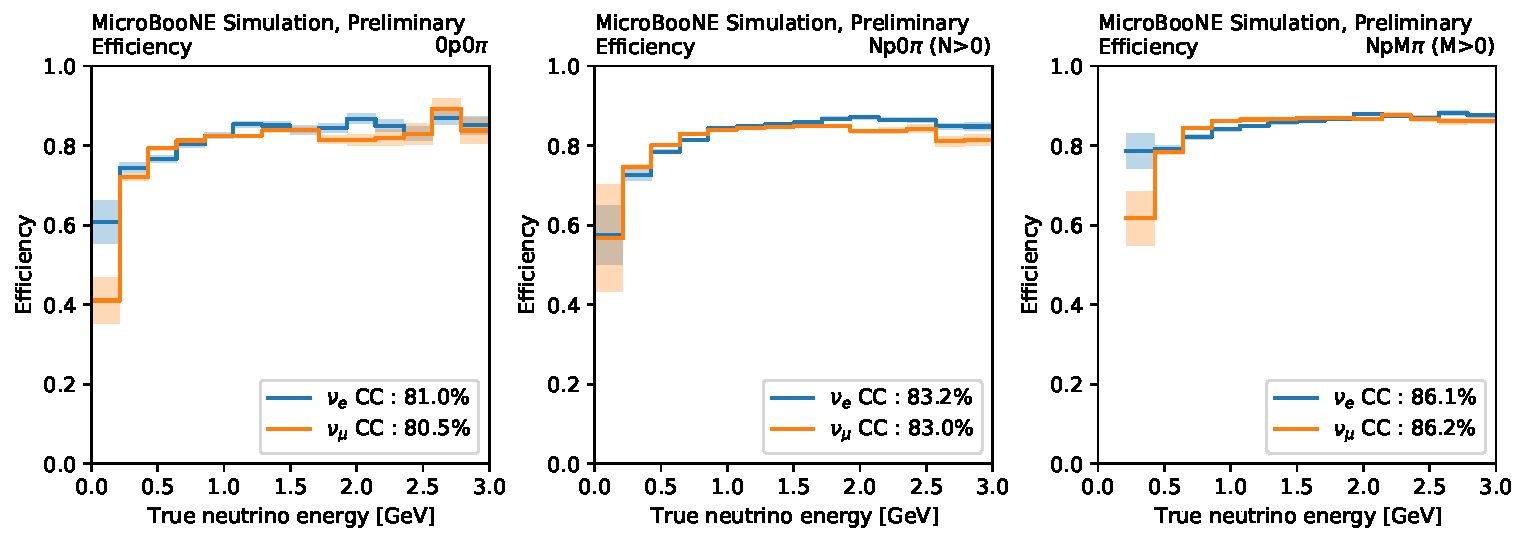
\includegraphics[width=0.75\textwidth]{NueCCsel/Images/truth/sliceID_eff.pdf}
    \caption{The performance of the \texttt{NeutrinoID} tool as a function of the true neutrino energy for the topologies considered in the \nuecc selection: \zpsel (left), \npsel (middle) and inclusive (right) channels. The energy range is \SIrange{0}{3}{\GeV} and the bin size is \SI{200}{\MeV}. The shaded areas correspond to the statistical errors arising from limiter simulated sample sizes.}
    \label{fig:sliceid_eff}
\end{figure}



\subsection{CRT Veto and Distance Tagger}
\label{sec:sliceID:CRT}
CRT tools are used in this analysis to boost cosmic rejection in the $\nu_{\mu}$ constrain selection, where the analysis-level containment requirement removes the concern of tagging exiting muons through CRT-based cuts. CRT-based cuts were explored for the $\nu_e$ selections as well but were ultimately found to be of little impact in the \npsel due to the powerful cosmic rejection achieved when requiring final-state protons. Considerable additional cosmic rejection was obatined with the CRT in the \zpsel, but the current analysis has chosen to not implement these cuts to avoid complications in mixing datasets from different runs with different selection requirements. Two specific cut concepts have been developed to make use of CRT information. Both are used in the $\nu_{\mu}$ and are described below.

\textbf{CRT Veto.} The CRT veto looks for a time coincidence between the scintillation light recorded in time with the 1.6 $\mu$s beam-spill (beam flash) and a CRT hit: if a CRT hit occurs within 1 $\mu s$ of the beam flash, the event is rejected. For this coincidence, only CRT hits with PE $>$ 100 p.e. are considered; we do not apply a constraint on the position of the flash or on the position of the CRT hit. 
The rejection power and efficiency of the CRT veto are calculated using the BNB external and the $\nu_e$ overlay samples, respectively. The BNB external rejection rate is $\sim$59\%. %,  and the $\nu_e$ passing rate greater than $\sim$94\% for all electron neutrino energies, even higher at low energies. \\

\textbf{CRT Distance Tagger.} 
The CRT Distance Tagger tool builds upon the standard Pandora neutrino vertex reconstruction and the CRT tagging of TPC tracks. A TPC track is tagged with a CRT hit association if the track projection onto a CRT panel and a CRT hit are close in space. 
To perform this association, the track projection to the CRT is calculated under the hypothesis that the associated particle crossed the TPC at the time registered by the CRT hit under consideration. More details on the CRT hit to TPC track matching are available in \cite{bib:CRTPresel_Technote}.  The CRT Distance Tagger checks the minimum distance between the reconstructed neutrino vertex and each track tagged with a CRT hit. If the minimum distance is less than 14 cm, the event is rejected. An example event tagged by this cut is shown in Figure~\ref{fig:crtdist00}.  With the CRT Distance Tagger an additional 19\% of off-beam backgrounds are rejected.% external passing rate is $\sim$81\%,  and the $\nu_e$ efficiency is greater than $\sim$96\% for all electron neutrino energies, even higher at low energies. \\
 
\begin{figure}[h!]
\centering
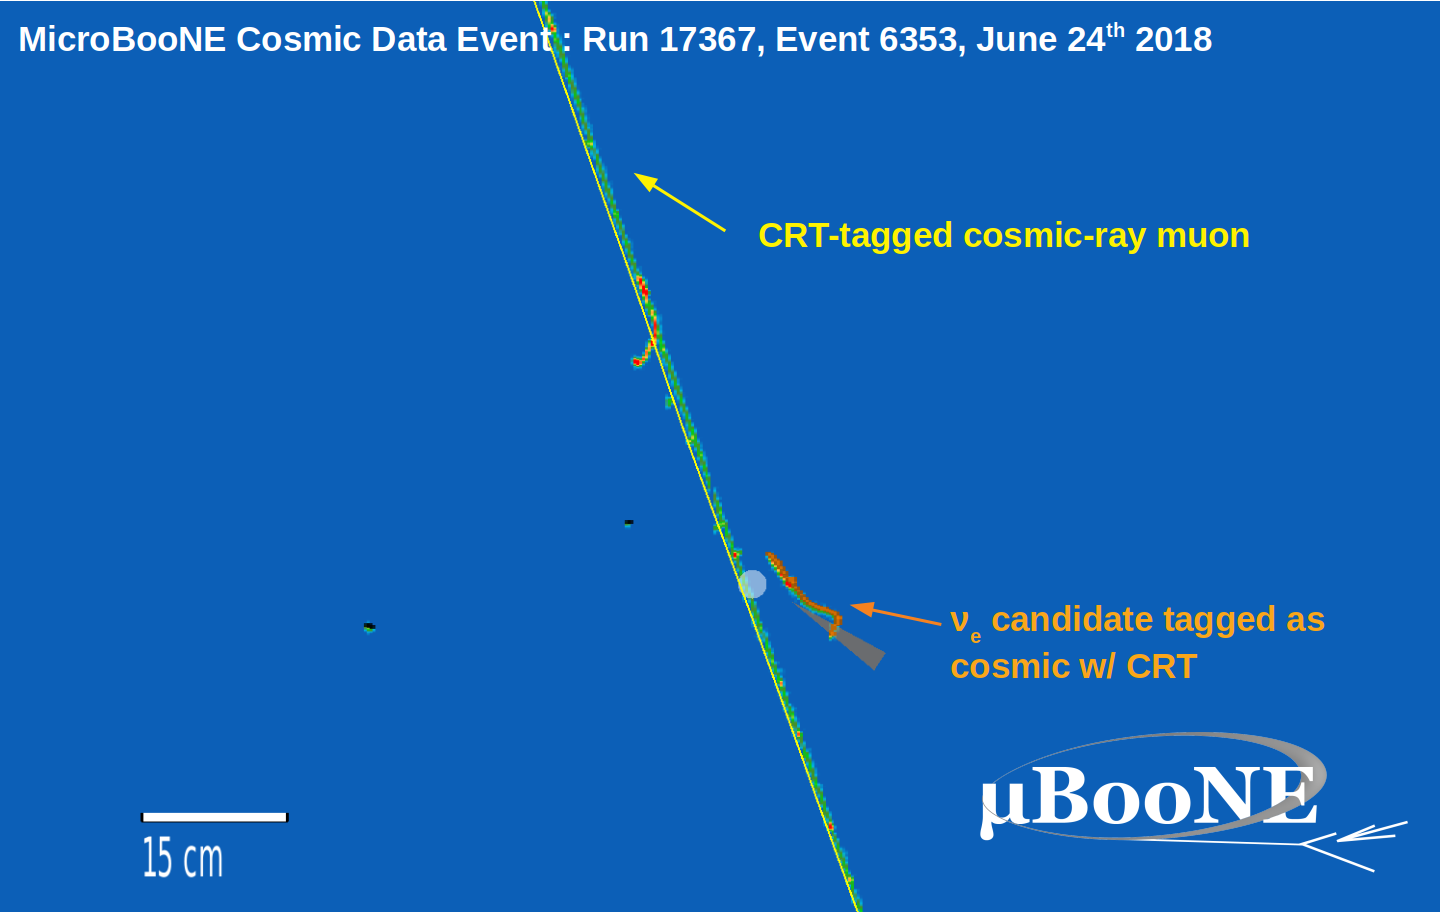
\includegraphics[width=0.4\textwidth]{NuId-Ch3/Images/crttagger_01.png}
\caption{Example $\nu_e$ candidate tagged as cosmic by the the CRT distance tagger. From the event one can see that the reconstructed EM shower is from EM activity that is associated with the cosmic muon.}
\label{fig:crtdist00}
\end{figure}

An overview of the impact of the CRT on cosmic rejection can be seen in Figure~\ref{fig:crt} where the beam-time distribution for the 8E18 POT Run 3 open data set is shown just after \texttt{NeutrinoID} (left), and after both \texttt{NeutrinoID} and CRT cosmic-tagging tools (including the CRT veto and distance tagger) have been applied (right). The EXT backgrounds drop by more than a factor of three.
Further details and a preliminary study of the CRT  impact on an electron neutrino pre-selection can be found in \cite{bib:CRTPresel_Technote}. 

\begin{figure}[ht] 
\begin{center}
    \begin{subfigure}[b]{0.4\textwidth}
    \centering
    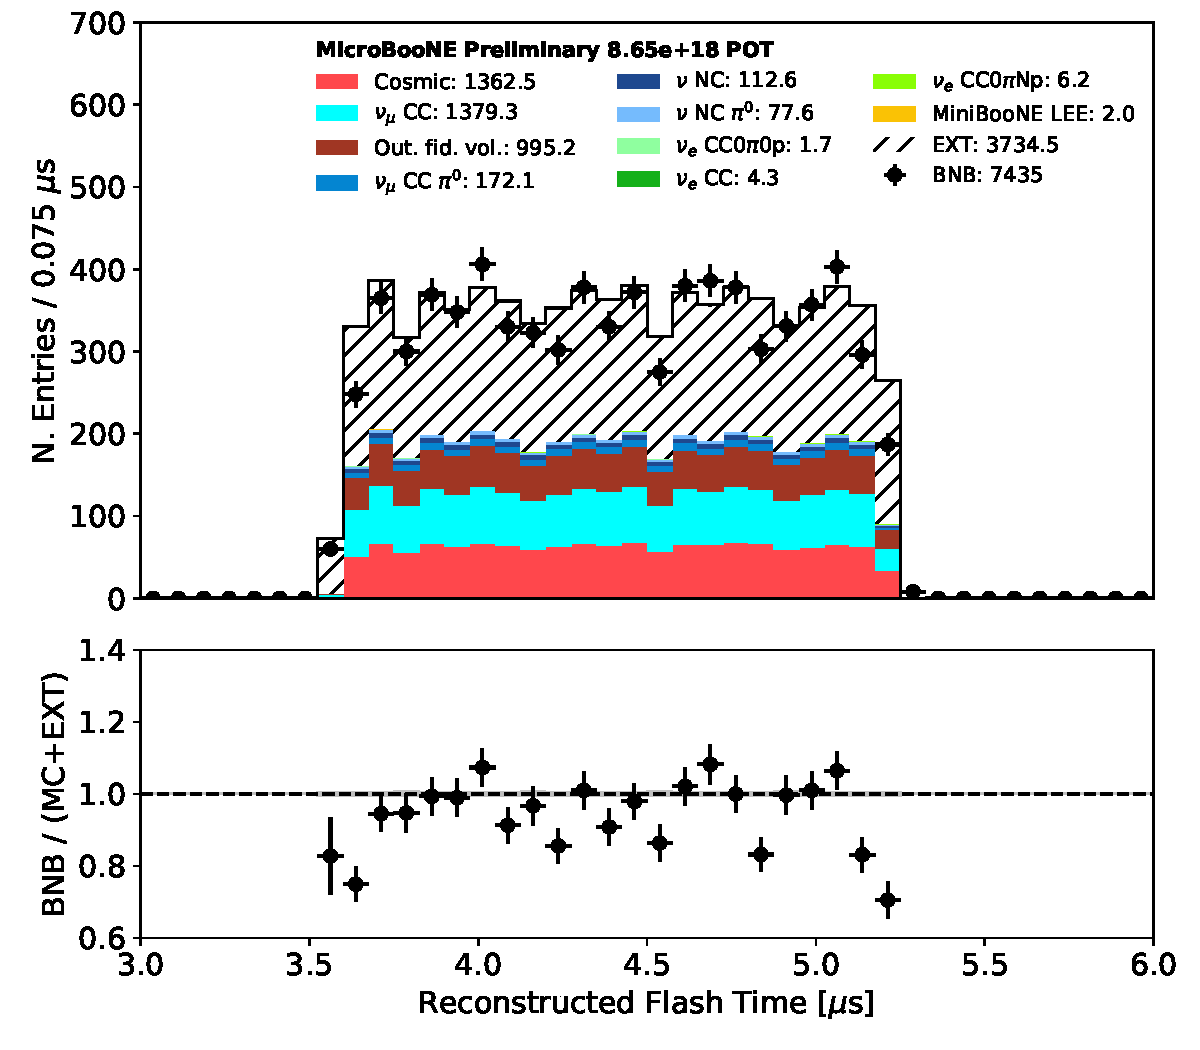
\includegraphics[width=1.00\textwidth]{NuId-Ch3/Images/flash_time_01152020.pdf}
    \caption{\label{fig:crt:pre} No CRT tools.}
    \end{subfigure}
    \begin{subfigure}[b]{0.4\textwidth}
    \centering
    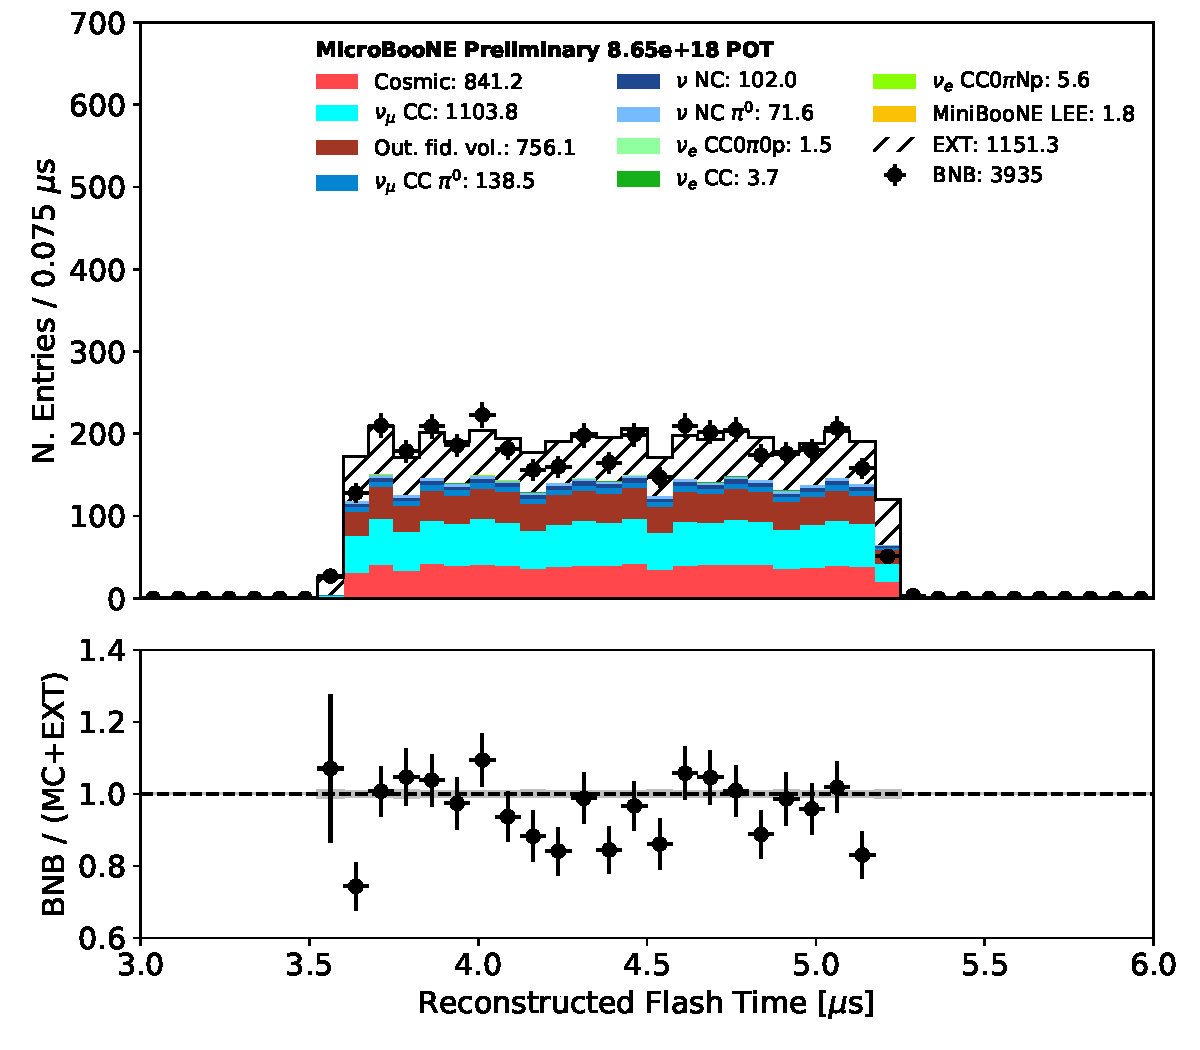
\includegraphics[width=1.00\textwidth]{NuId-Ch3/Images/flash_time_01152020_CRT.pdf}
    \caption{\label{fig:crt:post} With CRT tools.}
    \end{subfigure}
\caption{\label{fig:crt} Beam timing distribution before (a) and after (b) CRT tools have been applied. The EXT contribution is reduced by over a factor of three.}
\end{center}
\end{figure}

\newpage

\section{Neutrino Event Reconstruction}
\label{sec:NuEvtReco}
This section highlights the key aspects of the event reconstruction which allow for the classification of neutrino interactions: the track and shower reconstruction, the particle identification and the energy reconstruction.
\subsection{Track and Shower Reconstruction}
\label{sec:tkshreco}
The output of Pandora~\cite{bib:pandoraub} is organized in a hierarchy of reconstructed Particle Flow Particles (``PFParticles''), which describes the particle content in an observed event as a parent-daughter relationship chain. Final state PFParticles are 3D objects matching clusters of hits in at least two different planes.
Pandora classifies PFParticles as track-like or shower-like base on a Support Vector Machine (SVM) algorithm~\cite{bib:tkshsvm}, producing a score with values between 0 (shower-like) and 1 (track-like). PFParticles will be collected together based on physical proximity into slices, and ordered in a hierarchy (i.e. a Michel electron is the daughter of a muon, which is a daugther of a neutrino).

Pandora processes track-like PFParticles with a sliding linear fit procedure (described in~\cite{bib:pandoraub}) that returns the 3D position and direction at each point along the trajectory (where each point corresponds to a 2D hit). For each point the d$Q$/d$x$ and distance from the track-start are recorded using MicroBooNE's Calorimetry module. This procedure allows to accurately measure both d$x$, including small deflections due to the particle's trajectory and Space Charge Effect (SCE) offsets, and d$Q$, by incorporating MicroBooNE's full position- and field-dependent relative and absolute charge calibration. For tracks, the conversion from d$Q$/d$x$ to d$E$/d$x$ is performed by applying the inverse Modified Box recombination model~\cite{bib:tpccalibrationnote}.

We evaluate the energy and 3D direction of shower-like PFParticles with the same algorithm used for the $\pi^0$ reconstruction paper~\cite{bib:pi0reco}. The energy reconstruction accounts for various detector effects, including gain and recombination; corrections for reconstruction effects (hit threshold and imperfect clustering) will be described in Sec.~\ref{sec:ereco}. We also fit showers using a Kalman filter-based procedure~\cite{bib:shrtrackfitter} which aims at identifying the main trunk of the shower by rejecting hits that are longitudinally or transversely displaced from it; the output of this fit is a track object. Thus, the calorimetric tools described above become available for showers as well, with an important caveat: the conversion from d$Q$/d$x$ to d$E$/d$x$ is different for showers and tracks. For showers, a fixed recombination correction is applied assuming 2.1 MeV/cm energy loss for both the calculation of the trunk d$E$/d$x$ and for the total energy. In all cases, local variations in the electric field are accounted for.

By default, Pandora separates showers and tracks with a cut on the SVM score at 0.5; however, as will be described in later sections, in many cases we choose different cut values, i.e. tighter shower definition for the $\nu_e$ selection and looser for the $\pi^0$ control region.

The efficiency of Pandora's reconstruction on $\nu_e$ interactions is evaluated in figure~\ref{fig:nuereco:eff} as a function of true neutrino energy;  the efficiency for identifying the $\nu_e$ events as neutrino interactions is shown in black, and the efficiency for reconstructing $\nu_e$ interactions with a final-state EM shower in blue. The efficiency has a sharp upturn between 100 and 200 MeV, especially in the case when an EM shower is required, and levels off at 80\% and 60\% respectively for the two curves. 
\par At this stage in the analysis, the good efficiency for reconstructing $\nu_e$ events is offset by the very low signal-to-background for $\nu_e$ events in MicroBooNE's data, a consequence of the very small $\nu_e$ content of the beam. With no additional requirement on the reconstructed neutrino, the purity for $\nu_e$ interactions is 0.12\% (figure~\ref{fig:nuereco:sliceid}). After imposing a requirement of one reconstructed shower, the purity grows by almost an order of magnitude, to 1\% (figure~\ref{fig:nuereco:shower}). The $\nu$ background composition also changes significantly, with $\pi^0$ backgrounds moving from 14\% to 48\% of all backgrounds.

\begin{figure}[ht] 
\begin{center}
    \begin{subfigure}[b]{0.3\textwidth}
    \centering
    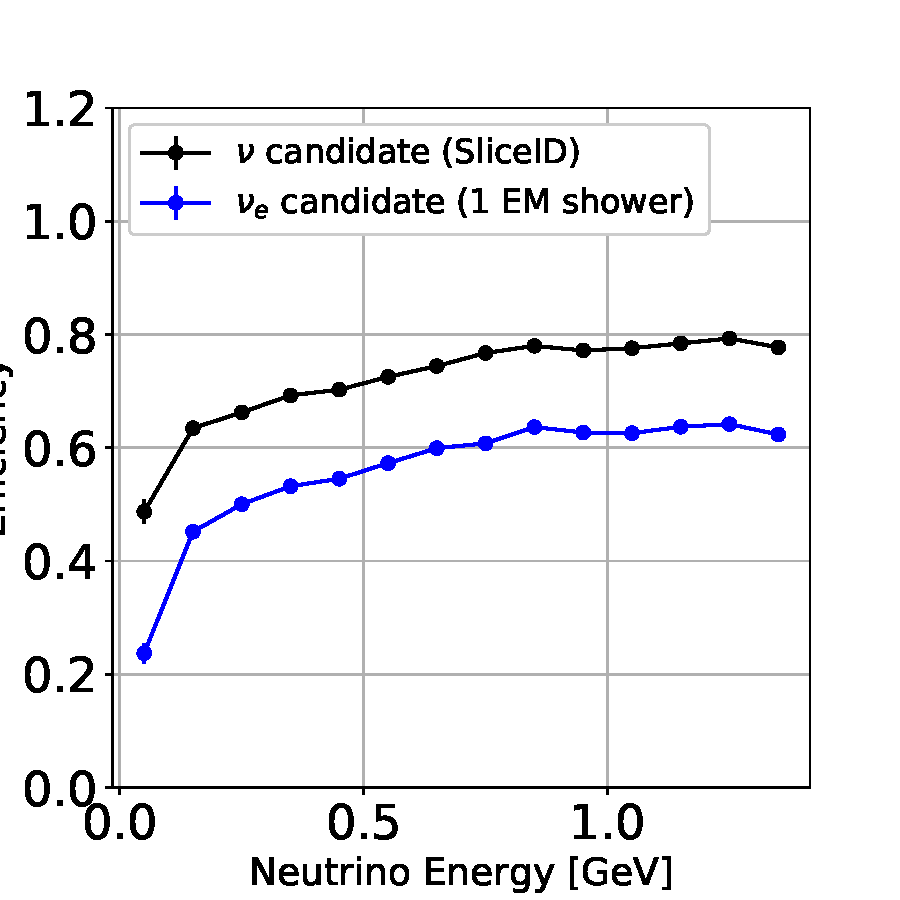
\includegraphics[width=1.00\textwidth]{nureco/nureco_RUN1.pdf}
    \caption{\label{fig:nuereco:eff} $\nu_e$ reco eff.}
    \end{subfigure}
    \begin{subfigure}[b]{0.31\textwidth}
    \centering
    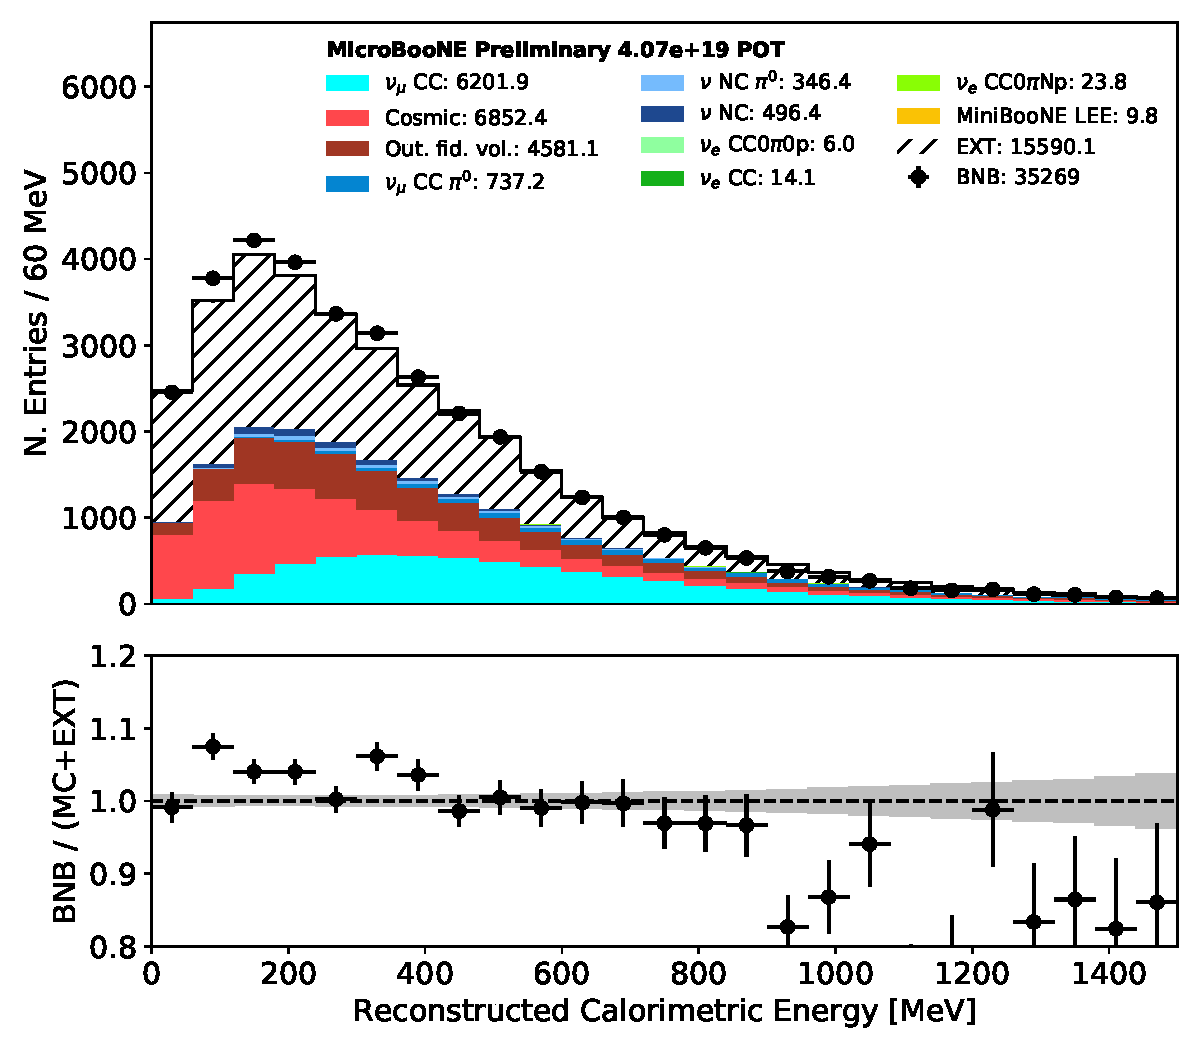
\includegraphics[width=1.00\textwidth]{nureco/NeutrinoEnergy2_01152020.pdf}
    \caption{\label{fig:nuereco:sliceid} after \texttt{SliceID}}
    \end{subfigure}
    \begin{subfigure}[b]{0.31\textwidth}
    \centering
    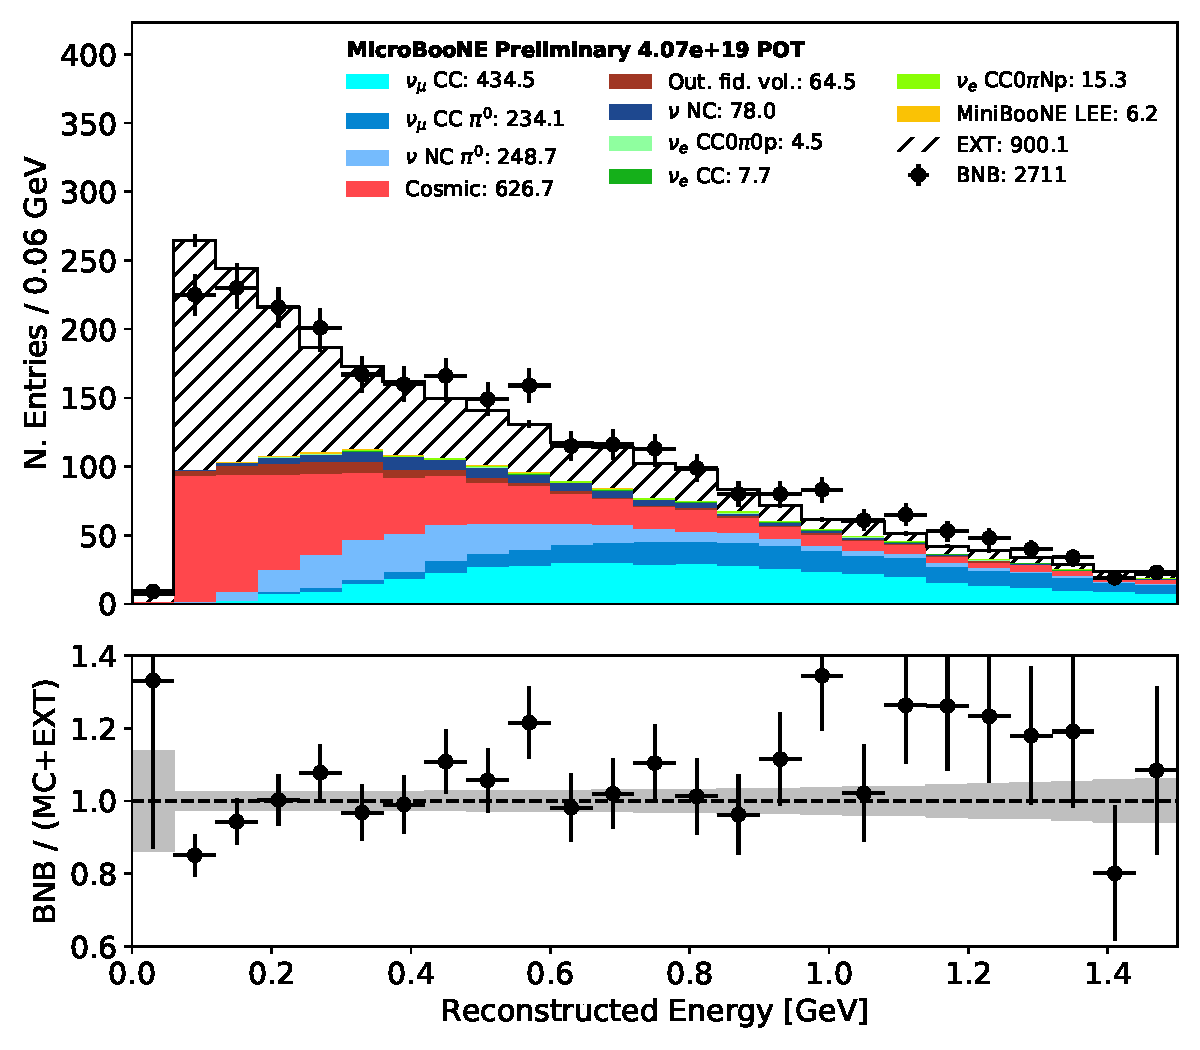
\includegraphics[width=1.00\textwidth]{nureco/reco_e_01152020.pdf}
    \caption{\label{fig:nuereco:shower} after shower requirement}
    \end{subfigure}
\caption{\label{fig:nuereco} \textcolor{blue}{ Y axis of figure a is cut off}}
\end{center}
\end{figure}

\par The next step in the analysis demands the development of a selection capable of isolating $\nu_e$ interactions rejecting the two order of magnitude larger background rates from $\nu_{\mu}$ neutrinos. This selection will make use of PID and topological information described in the next sections. The strong level of background rejection needed to isolate signal events will inevitably lead to a lower selection efficiency.

\subsection{Particle Identification}
% GC: this part is now in the previous subsection
%In the neutrino slice, every PFParticle is reconstructed in three different ways:
%\begin{itemize}
%    \item Track, using the standard Pandora Track reconstruction
%    \item Shower, using the standard Pandora Shower reconstruction (is there any modification on top of this?)
%    \item Track-fitted shower, using a dedicated track fitting tool which aims at identifying the main branch of %the shower and fit it as a track. As a result, all the tools developed for the track become available for the %tracks too. For example, for each track-fitted shower, a recob::track and a anab::calorimetry objects are available.
%\end{itemize}
Particle identification is performed with different tools depending on whether the particle is selected as a track- or shower-candidate.
If the PFParticle has been selected as a track-like object, the identification is performed using the Calorimetry Likelihood tool, which results in the variable Log Likelihood Ratio PID (LLR), see section~\ref{subsec:loglikelihoodpid}.
If the PFParticle has been selected as an electron or photon candidate, the identification is performed using several variables described in \ref{subsec:egammaspearation}.
%It is noteworthy that this particle identification consists of one or multiple variables, available for the specific PFParticle, that may or may not depend on \textcolor{blue}{additional information from} the rest of the slice. 
%For example, the shower d$E$/d$x$ depends only on the PFParticle itself, whereas the track-shower separation relies also on additional objects identified in the slice.
Notably, additional information provided by the rest of the slice may be used for the particle identification 
depending on the specific PFParticle. For example, while the shower d$E$/d$x$ depends only on the PFParticle itself, the track-shower separation relies also on additional objects identified in the slice.

When choosing the cut values for PID variables, we account not only for the efficiency and mis-identification achievable to distinguish two kinds of particles (e.g. electrons from photons), but also for the mixture of backgrounds specific to the considered topology: e.g. \textcolor{blue}{add example}. 

%The value of the cuts applied on these variables depends not only on the general level of efficiency and mis-identification achievable to distinguish two kind of particles (electrons from photons, for example), but also on the mixture of backgrounds specific to selection the analyzer is performing.





\subsubsection{Log Likelihood Ratio  PID \textcolor{green}{Nico, P.R. David, Elena}}
\label{subsec:loglikelihoodpid}

For track-like particles, the particle identification is performed looking at the profile of the deposited charge per unit length (d$E$/d$x$). The scope of track PID is to identify the particle type which originated a given track object. In this analysis, we limit PID to a binary classification problem, i.e.  how to distinguish protons from muons. We disregard further classification because kaons are rarely produced in neutrino interactions at the energy of interest, whereas pions are very difficult to distinguish from muons using calorimetry information only.
Additional information, such as possible hadronic reinteractions or Michel electrons, can be powerful to perform particle identification but is not leveraged in this analysis.

The expected distribution of the $dE/dx$ is modeled for each particle type and for each plane, as a function of two variables: the residual range ($rr$), and the pitch as
\[ p(dE/dx | \text{type}, \text{plane}, \text{rr}, \text{pitch}). \]
The residual range is the distance of a given space point from the end of the track, measured along the track trajectory, while the pitch is the length over which the charge measured on a given wire has been deposited.
The expected distribution is modeled for each plane independently, and for the two kinds of particles under study, protons and muons.
Multiple effects enter in the model of this distribution.
The first effect is what we want to leverage:  the average d$E$/d$x$ at a given residual range depends on the particle's mass, as seen by integrating the Bethe-Bloch function for different masses.
Secondly, the fluctuations of the d$E$/d$x$ depend on the pitch. These fluctuations are intrinsically stochastic: the longer the length over which the charge is averaged, the smaller the fluctuations.
Furthermore, detector effects such as recombination, signal deconvolution, and hit reconstruction add a non-linear response and smearing; this response depends on both the true deposited charge and the pitch, and lacks an analytic model. For this reason, the expected distribution of $dE/dx$ is built starting from the simulation.
The performance of the particle identification improves as the model for the  $dE/dx$ distribution becomes more accurate.
The model for $dE/dx$ is built by considering well reconstructed tracks\footnote{ We define a ``well reconstructed track" a track whose completeness and purity are both above 90\%, where completeness measures how much of the true particle's  deposited charge is reconstructed in the track and purity measures how little spurious charge enters the track reconstruction. }, well contained within a fiducial volume, and backtracked to protons and muons.
The binning of the probability density function (pdf) is the following:
\begin{itemize}
    \item $dE/dx$: $[0, 0.5, 1, 1.5, 2, 2.5, 3, 3.5, 4, 4.5, 5, 5.5, 6, 6.5, 7, 7.5, 8, 9, 10, 12, 15, 20, 25, 30, 35, 40, 45, 50]$ MeV/cm
    \item residual range: $[0., 2, 4, 7, 10, 15, 20, 30, 50, 100, 300, 2000]$ cm
    \item pitch: $[0.3, 0.6, 1, 1.5, 3, 30]$ cm
\end{itemize}
A couple of examples of the pdf are provided in figure \ref{fig:llr_pid_pdf_example}, for two different bins in residual range and pitch.

\begin{figure}[ht] 
\begin{center}
    \begin{subfigure}[b]{0.48\textwidth}
    \centering
    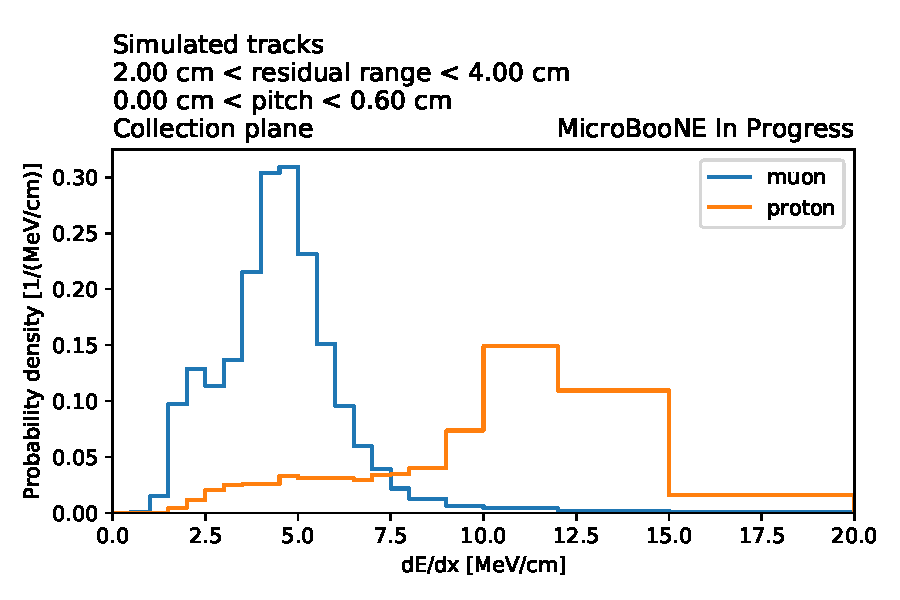
\includegraphics[width=1.00\textwidth]{llrpid/plane_2_rr_30_pitch_03.pdf}
    \end{subfigure}
    \begin{subfigure}[b]{0.48\textwidth}
    \centering
    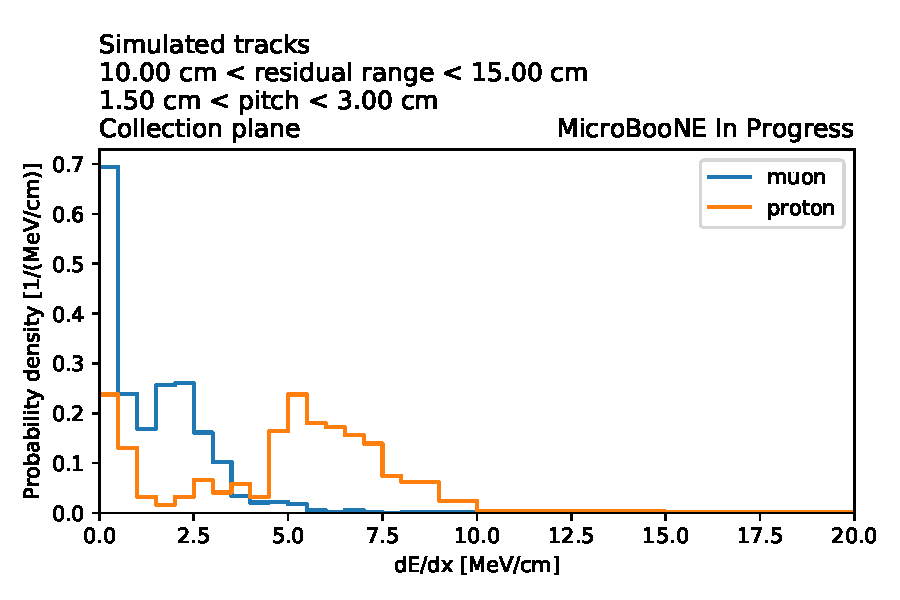
\includegraphics[width=1.00\textwidth]{llrpid/plane_2_rr_125_pitch_225.pdf}
    \end{subfigure}
\caption{Comparison of the expected distribution of $dE/dx$ for muons (blue) and protons (orange), for two different bins in residual range and pitch (left and right).}
\label{fig:llr_pid_pdf_example}
\end{center}
\end{figure}

For a given track, we consider the calorimetry objects on all three planes. For each plane, the $dE/dx$, residual range, and pitch vectors are used to compute the likelihood of each particle type,
\[ \mathcal{L}(\text{type} | \text{plane}, dE/dx_{i = 1, ..., N},   \text{rr}_{i = 1, ..., N}, \text{pitch}_{i = 1, ..., N}) = \prod_{i=1}^N p(dE/dx_i | \text{type}, \text{plane}, \text{rr}_i, \text{pitch}_i) \]
where the index $i=1, ..., N$ runs over each hit for the considered plane.
The combination of the three planes happens in a straightforward way, by taking the product of the three likelihoods, or summing up the log-likelihoods,
\[ p(dE/dx | \text{type}, \text{plane}, \text{rr}, \text{pitch}). \]
In order to perform the classification task, the likelihood ratio test statistic is chosen:
\[ T(dE/dx, \text{rr}, \text{pitch}) = \mathcal{L}(\text(muon)| dE/dx, \text{rr}, \text{pitch}) /  \mathcal{L}(\text(proton)| dE/dx, \text{rr}, \text{pitch}). \]
An example of the distribution of these variable, normalized between -1 and 1, is given in figure \ref{fig:llr_pid_uvy_example}, for tracks contained in a fiducial volume, and backtracked to muon, proton, or cosmic.

The likelihood ratio, as defined above can be proven to be the most powerful statistical test, i.e. the one with the smallest mis-identification rate for any given value of the efficiency.
Any mis-modeling in the simulation used to build the likelihood produces a loss of power, as the test would not be the most powerful one.
Systematic uncertainties arise from the fact that the measured distribution of $dE/dx$ in the data may differ from the simulation, or because the properties of the tracks we consider may not be properly simulated, such as angular or length distributions.
This behaviour is qualitatively present in all the PID methods.

In a MC sample of contained protons and muons used to test the performance, this PID variable is able to reach 94\% muon efficiency, with 10\% proton mis-ID rate.

\begin{figure}[ht] 
    \centering
    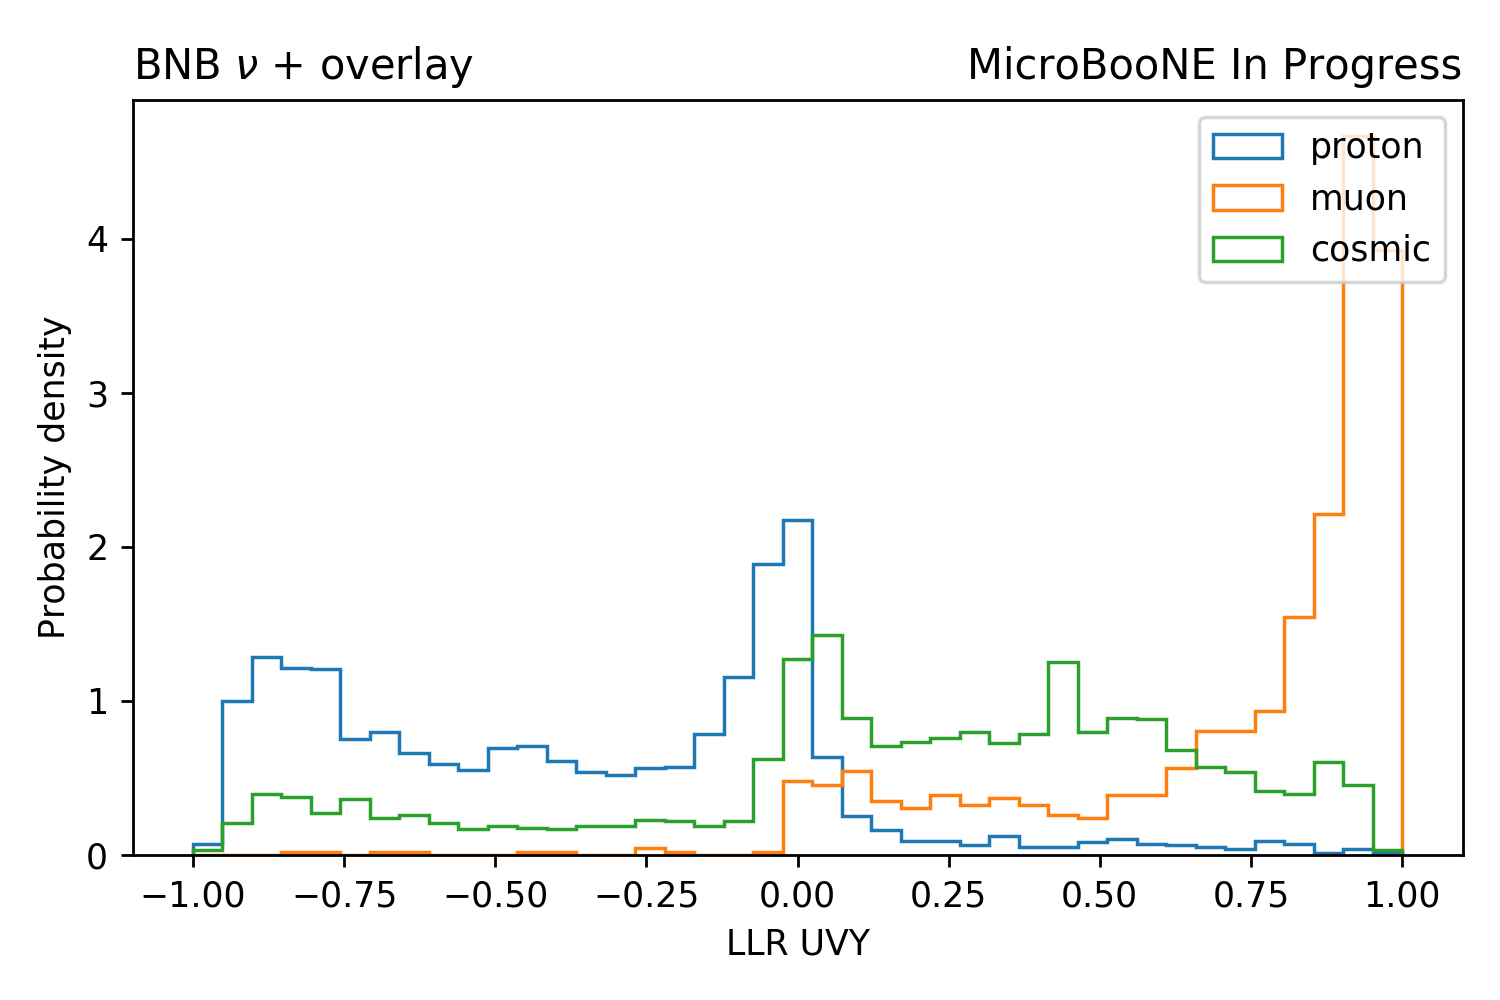
\includegraphics[width=0.7\textwidth]{llrpid/llr_012_n.png}
    \caption{Distribution of the log-likelihood-ratio PID variable for tracks well contained in a fiducial volume, and backtracked to muon (orange), proton (blue), or cosmic (green).}
    \label{fig:llr_pid_uvy_example}
\end{figure}




\subsubsection{$e$/$\gamma$ Separation \textcolor{green}{David, P.R Elena}}
\label{subsec:egammaspearation}
\par Distinguishing electron from photon EM-showers is one of the crucial steps required to perform a measurement of $\nu_e$ interactions in the BNB beam. Photon backgrounds to a $\nu_e$ measurement are largely caused by neutrino interactions with $\pi^0 \rightarrow \gamma\gamma$ in the final state; this topology dominates the $\nu_e$ event rate by approximately an order of magnitude. Three key features distinguish events with $\pi^0$ induced photon showers from $\nu_e$ interactions: (a) the presence of two final state EM showers. (b) the non-zero conversion distance separating the neutrino interaction vertex from the shower start point, and (c) the calorimetric separation via $dE$/$dx$ due to the overlapping ionization segment of $e^+$/$e^-$ pair-conversions through which most $\gamma$ showers manifest themselves. Figure~\ref{fig:egammasep} shows how, at reconstruction level, each of these features can aid in $e$/$\gamma$ separation. This section describes how each of the items above is utilized in the analysis on a technical level, what performance is obtained, and what challenges (both physics- and reconstruction-driven) are encountered when leveraging these variables.

\begin{figure}[ht] 
\begin{center}
    \begin{subfigure}[b]{0.31\textwidth}
    \centering
    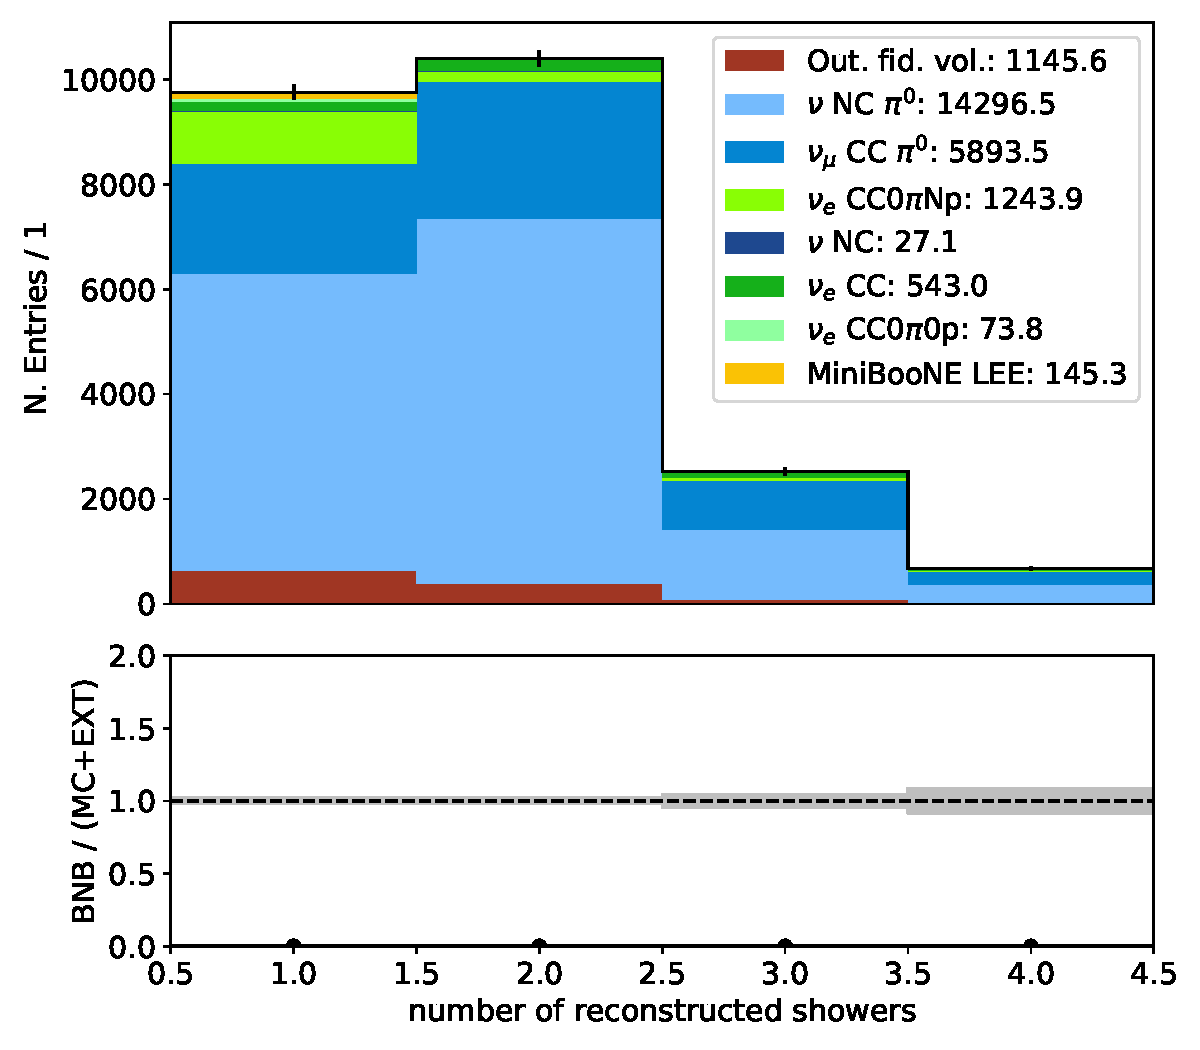
\includegraphics[width=1.00\textwidth]{egamma/n_showers_contained_01022020.pdf}
    \caption{number of reconstructed showers}
    \end{subfigure}
    \begin{subfigure}[b]{0.31\textwidth}
    \centering
    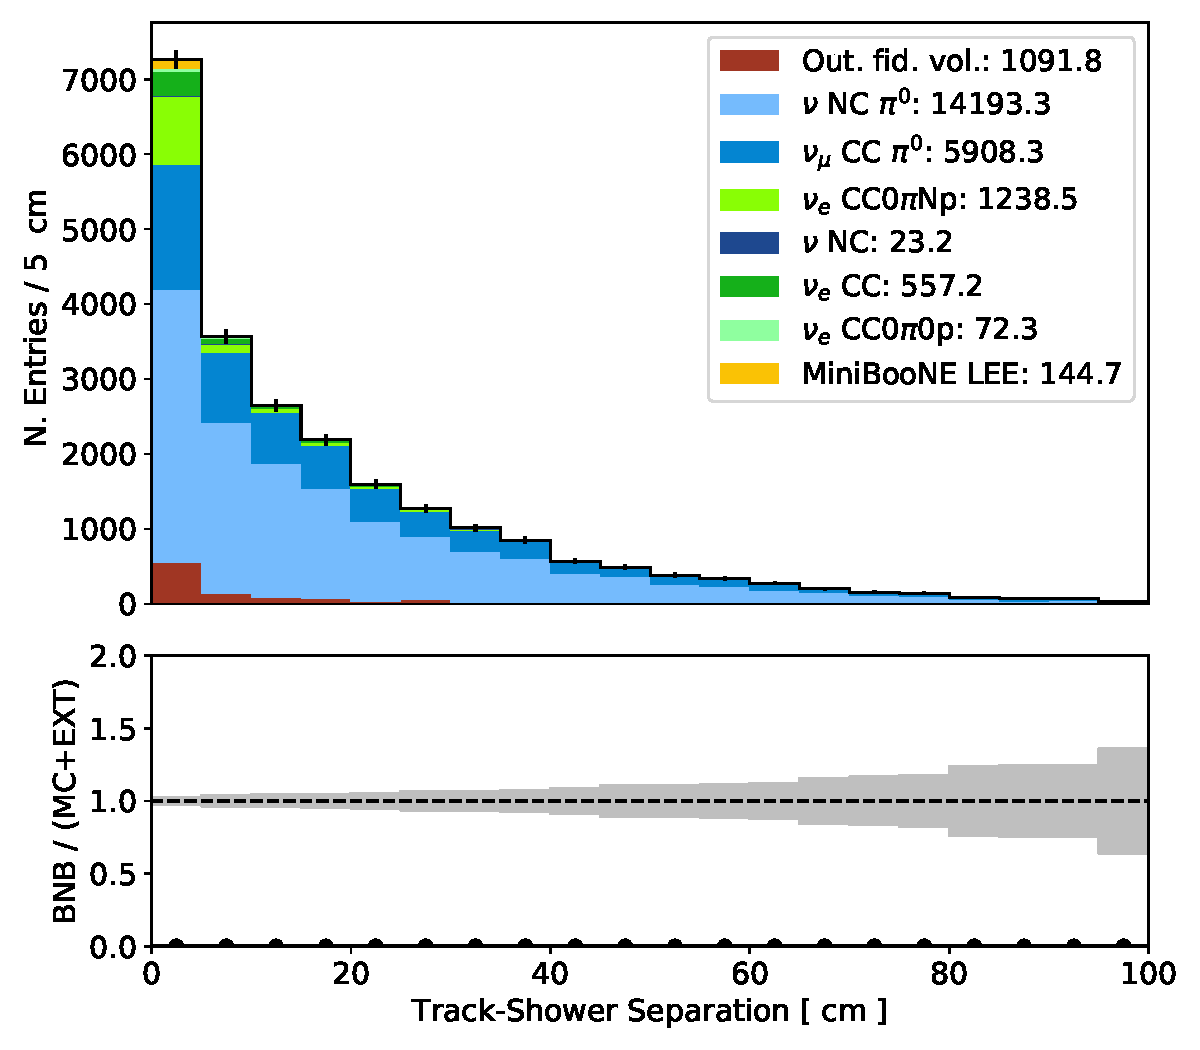
\includegraphics[width=1.00\textwidth]{egamma/tksh_distance_01022020.pdf}
    \caption{track-shower separation}
    \end{subfigure}
    \begin{subfigure}[b]{0.31\textwidth}
    \centering
    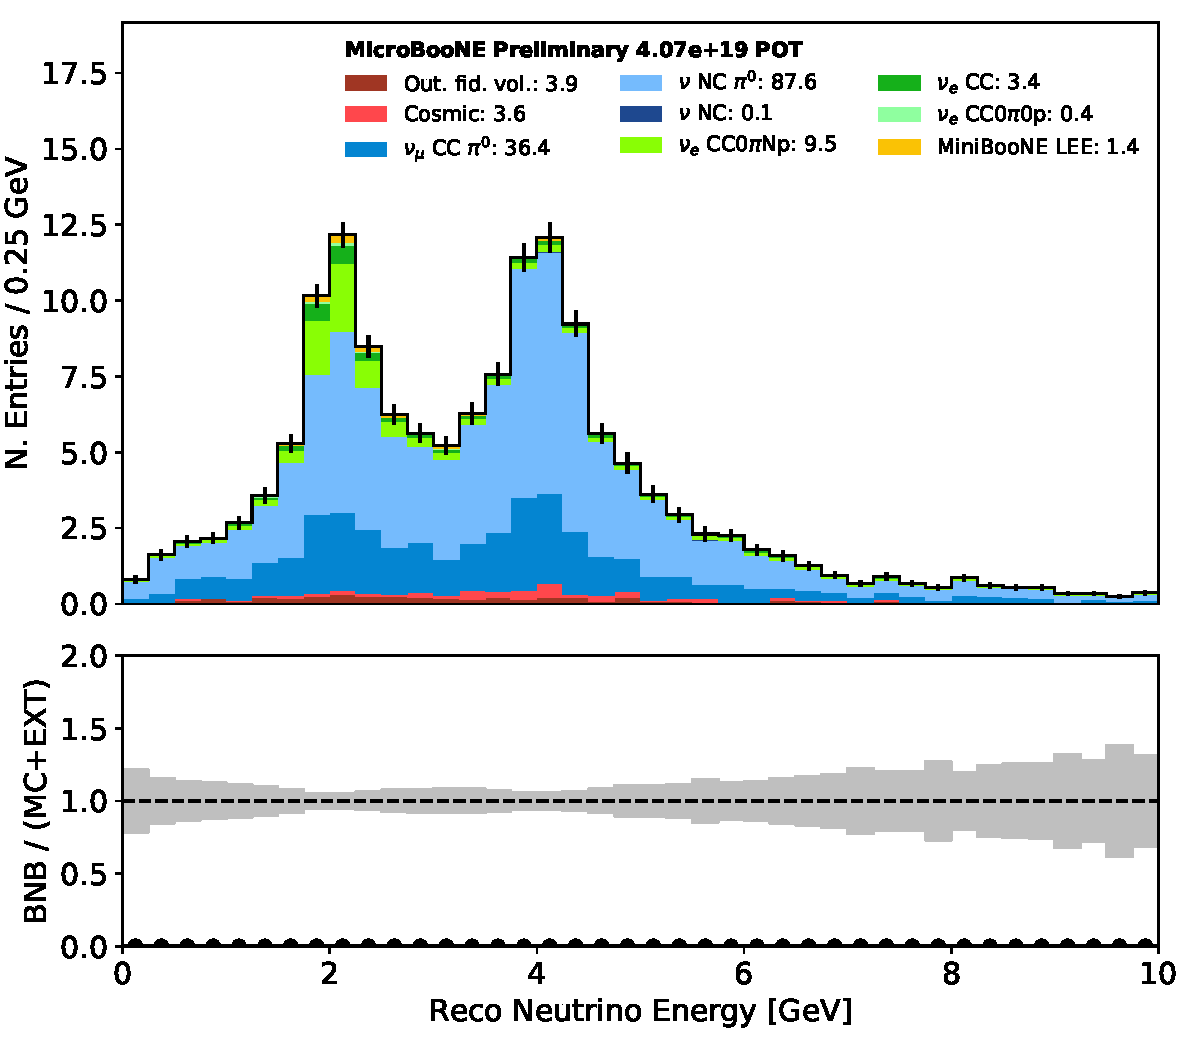
\includegraphics[width=1.00\textwidth]{egamma/shr_tkfit_dedx_Y_01192020.pdf}
    \caption{\label{fig:egammasep:dedx} reconstructed shower $dE$/$dx$}
    \end{subfigure}
\caption{\label{fig:egammasep}Comparison of simulated $\nu_e$ (green) vs. $\nu_{\mu} \rightarrow \pi^0 + X$ (blue) for the three discriminating variables of (a) number of showers, (b) vertex distance, and (c) $dE$/$dx$. Distributions are POT-normalized but contain only $\nu_e$ or $\pi^0$ events (no on/off-beam data distributions).}
\end{center}
\end{figure}

\par \textbf{two-shower requirement} Requiring a single reconstructed shower retains 68\% of $\nu_e$ interactions (with no $\pi^0$ in the final state) while removing 61\% of $\nu_{\mu}$ events with at least one $\pi^0$ in the final state. The fraction of selected $\nu_e$s grows to 79\% when looking below 800 MeV of true energy (the focus of this analysis). Rejection of $\nu_e$s is largely due to events where the electron shower is reconstructed as two separate EM showers, often closely aligned in 3D. Events with final state $\pi^0$s are reconstructed with a single EM shower in the final state because either the second photon escapes the TPC active volume completely (irreducible) or because the second shower is not reconstructed. The dominant causes of this second case are (1) highly-boosted $\pi^0$ decays, in which two aligned photons are merged into one shower and (2) photons which go undetected, often low in energy (below 100 MeV). Additional discriminating variables which aim to recover the reconstruction-related mis-ID of (1) and (2) are utilized in the analysis and presented in Sec.~\ref{sec:nueselection:inputs}.
\par \textbf{track-shower separation} For events where hadronic activity at the neutrino interaction vertex (i.e. final-state protons) is visible, a clear gap between the vertex and the shower start-point can be used to reject $\gamma$ backgrounds. This is a powerful background mitigation tool in the 1$e$N$p$ $\nu_e$ selection. Two factors determine the performance of such a tool: the ability to detect protons and other hadronic activity at the vertex and the accuracy with which the shower start-point is reconstructed. The shower start-point reconstruction accuracy determines the level of background rejection obtainable, as $\gamma$ showers lead to an exponential conversion-distance distribution. \textcolor{blue}{A 1 cm vs. 5 cm track-shower separation cut leads to 95\% vs 74\% mis-ID respectively, but causes a drop in selection efficiency for 1$e$N$p$ events from 72\% to 28\%. I don't think I understand these numbers... because what  I'm understanding is not logical: if I reject events with a 1 cm or more gap, I keep 72\% of nues and 95\% of photons. If I reject events with a 5 cm or more gap, I keep only 28\% nue and 75\% photons. This is completely counter intuitive, what am I getting wrong?  } This is a consequence of the sub-optimal vertex reconstruction accuracy for low-energy $\nu_e$ interactions. In order to enhance the ability to isolate $\nu_e$ events in the 1$e$N$p$ selection through vertex-displacement, different metrics are used to measure the presence of a gap between an electron and proton candidate. These will be described in section~\ref{sec:nueselection:inputs}. It is important to note that this background mitigation strategy is not applicable to single-electron searches, which are an important contribution to $\nu_e$ interactions, especially in the low-energy regime.
\par \textbf{shower d$E$/d$x$} The majority of photons manifest themselves in the TPC through the ionization released by the $e^+$/$e^-$ pair produced via pair-conversion. The electron-positron pair is highly aligned and overlaps on the mm-scale, leading to a doubly-ionizing charge-segment compared to electron showers. To measure this, we use the track fit of the main shower trunk and the calorimetric tools as described in Sec.~\ref{sec:tkshreco}. 
%with a modified version of the MicroBooNE track-fitter~\cite{bib:shrtrackfitter} and for each point along a track the d$Q$/d$x$  and distance from the shower-start are recorded using MicroBooNE's Calorimetry module. This procedure allows to accurately measure d$x$, including small deflections due to the electron's trajectory and SCE offsets, and d$Q$, by incorporating MicroBooNE's full position- and field-dependent relative and absolute charge calibration. From d$Q$/d$x$, d$E$/d$x$ is calculated assuming a fixed recombination correction assuming 2.1 MeV/cm energy loss, but accounting for local variations in the electric field. 
The distinctive 4 MeV/cm population expected for $\gamma$ showers is visible in figure~\ref{fig:egammasep:dedx}. The main limitation to $e$/$\gamma$ separation via d$E$/d$x$ is the large fraction of photons reconstructed with a d$E$/d$x$ of less then 3 MeV/cm (23\% of $\pi^0$ events fall in the 1-3 MeV range). This is due both to mis-reconstructed events, for which the start-point is incorrectly reconstructed by more than one or two cm, and to events where the photon shower's energy loss-profile is not as clearly distinguishable from that of a single electron. While the relative contribution of these two sources is still under determination, the second causes a significant mis-ID rate, and is largely associated to lower-energy $\gamma$ showers for which the production of a highly asymmetric electron-positron pair where one of the electrons is barely visible is more frequent. The impact of shower energy on the measured d$E$/d$x$ for a $\gamma$ shower is shown in figure~\ref{fig:dedxgammas:energy}. Below 100 MeV, where most $\gamma$ showers in the BNB are produced, the reconstructed d$E$/d$x$ is electron-like. The impact of distance from the shower start-point on whether d$E$/d$x$ is reconstructed to be 2 or 4 MeV/cm is also important, as can be seen in figure~\ref{fig:dedxgammas:dist}. This is particularly true for low-energy asymmetric pair-production events, and motivates utilizing 
d$E$/d$x$ information at different distances from the shower start-point for $e$/$\gamma$ separation.
\begin{figure}[H] 
\begin{center}
    \begin{subfigure}[b]{0.45\textwidth}
    \centering
    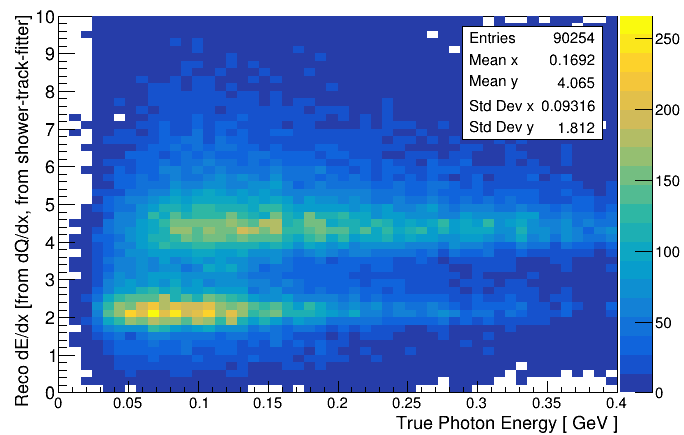
\includegraphics[width=1.00\textwidth]{egamma/dedx_vs_energy_gamma.png}
    \caption{\label{fig:dedxgammas:energy} d$E$/d$x$ vs. distance from shower start-point for $\gamma$ showers \textcolor{blue}{wrong caption}}
    \end{subfigure}
    \begin{subfigure}[b]{0.45\textwidth}
    \centering
    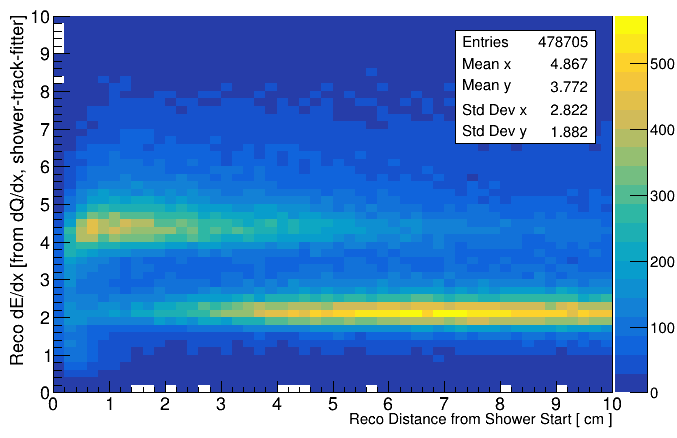
\includegraphics[width=1.00\textwidth]{egamma/dedx_vs_dist_gamma.png}
    \caption{\label{fig:dedxgammas:dist} d$E$/d$x$ vs. distance from shower start-point for $\gamma$ showers}
    \end{subfigure}
\caption{\label{fig:dedxgammas}}
\end{center}
\end{figure}



%\newpage

\subsection{Energy Reconstruction \textcolor{green}{Giuseppe + David... (PR Elena)}}
\label{sec:ereco}
\par Energy reconstruction is performed thought calorimetry for EM showers and through a measurement of a track's range for contained muons and protons. For \textcolor{blue}{should we add "uncontained"} muons, multiple Coulomb scattering (MCS) is also used to estimate the muon energy. The energy resolution obtained for different particles is reported in table~\ref{tab:eres}. More information on each particle's energy resolution is reported in figure~\ref{fig:eres:particle} where the 2D reconstructed vs. true energy distribution (in log-scale) is shown on the left, next to a plot of energy resolution vs. true energy on the right. The energy resolution reported here is obtained from a Gaussian plus one-sided exponential fit to the distribution $[E_{\rm reco}-E_{\rm true}] / E_{\rm true}$, see figures \ref{fig:eres:elec:binned}. The resolution reported refers only to the Gaussian width $\sigma$ extracted in the fit, and therefore does not account for negative tails, which are significant in the case of EM shower energy reconstruction, and described below.


\begin{table}[H]
\centering
  \begin{tabular}{ | c | c |  }
    \hline
    particle & kinetic energy resolution  \\ \hline
    proton & 4\% at 100 MeV 1\% at 200 MeV \\ \hline
    muon (range) & 3\%  \\ \hline
    muon (MCS) & $\frac{4.7\%}{\sqrt{E/{\rm GeV}}} \otimes \frac{2.8\%}{E/{\rm GeV}} \otimes 0.0\% \text{\textcolor{blue}{this is fairly confusing, especially the 0.0\%, can we add a reference, or an explaination?}}$  \\ \hline
    electron & 15\%  \\
    \hline
    
  \end{tabular}
  \caption{\label{tab:eres} Energy resolution for different particle species.}
 \end{table}
 
 \par For EM showers, the calorimetric energy reconstruction response has a significant non-Gaussian component, as well as a large bias. Both effects are attributable to reconstruction effects associated with under-clustering of charge. The energy bias is found to be 20\% and approximately flat in energy, and motivates a definition of a corrected shower energy, defined as $E_{\rm corrected} = E_{\rm calorimetry} / 0.8$. The non-Gaussian response for EM energy reconstruction can be modeled through a Gaussian plus one-sided exponential distribution. Figure~\ref{fig:eres:elec:binned} shows in different bins of true energy the fractional energy response and a fit to a Gaussian plus one-sided exponential function. The residual energy bias, after the 20\% correction applied, is of order $3-8$\%. 
 
\begin{figure}[ht]
\begin{center}
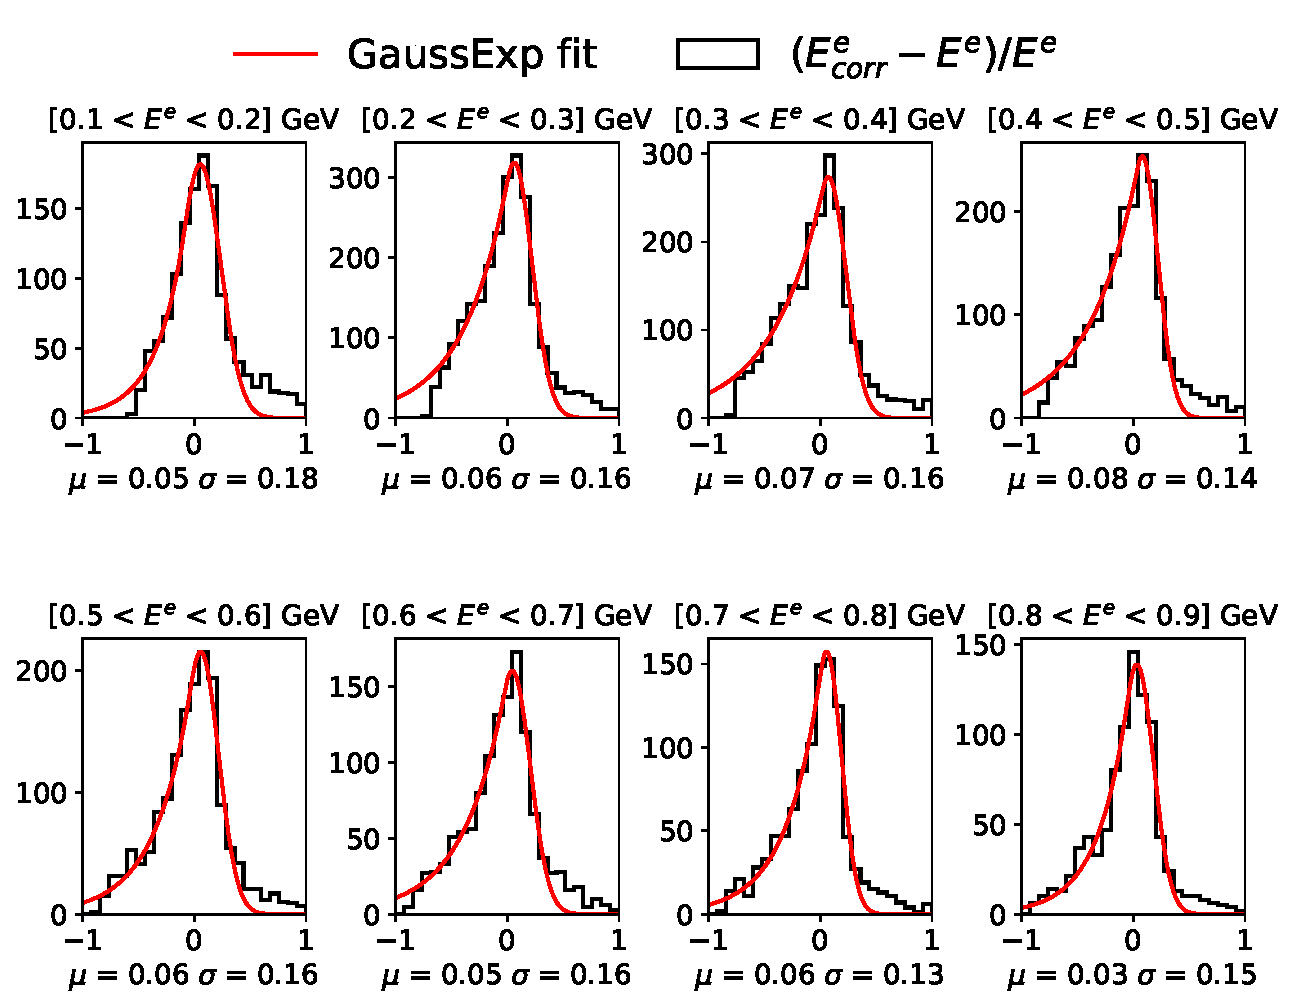
\includegraphics[width=0.75\textwidth]{ereco/elec_eres_binned.pdf}
\caption{\label{fig:eres:elec:binned}Energy resolution for electron showers.}
\end{center}
\end{figure}
 
\clearpage

\begin{figure}[H] 
\begin{center}
    \begin{subfigure}[b]{0.4\textwidth}
    \centering
    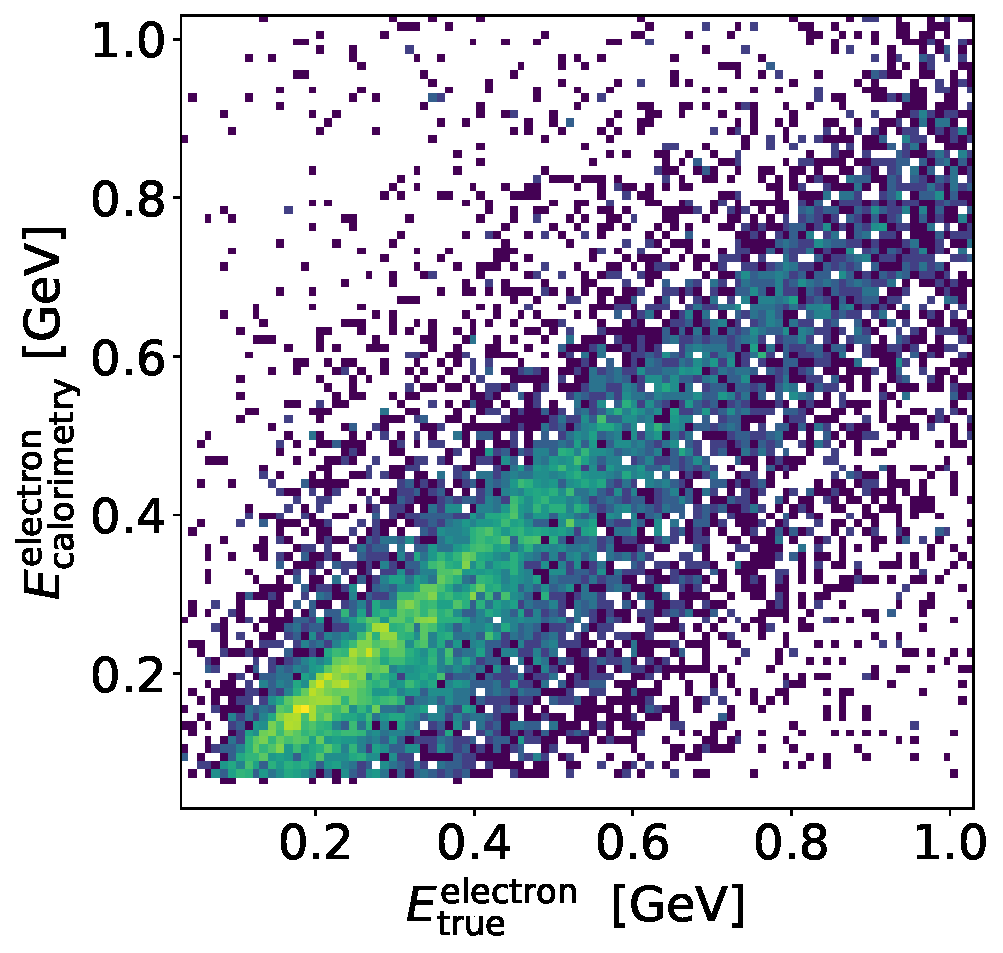
\includegraphics[width=1.00\textwidth]{ereco/electron_eres2D.pdf}
    %\caption{\label{fig:eres:elec:2d} }
    \end{subfigure}
    \begin{subfigure}[b]{0.38\textwidth}
    \centering
    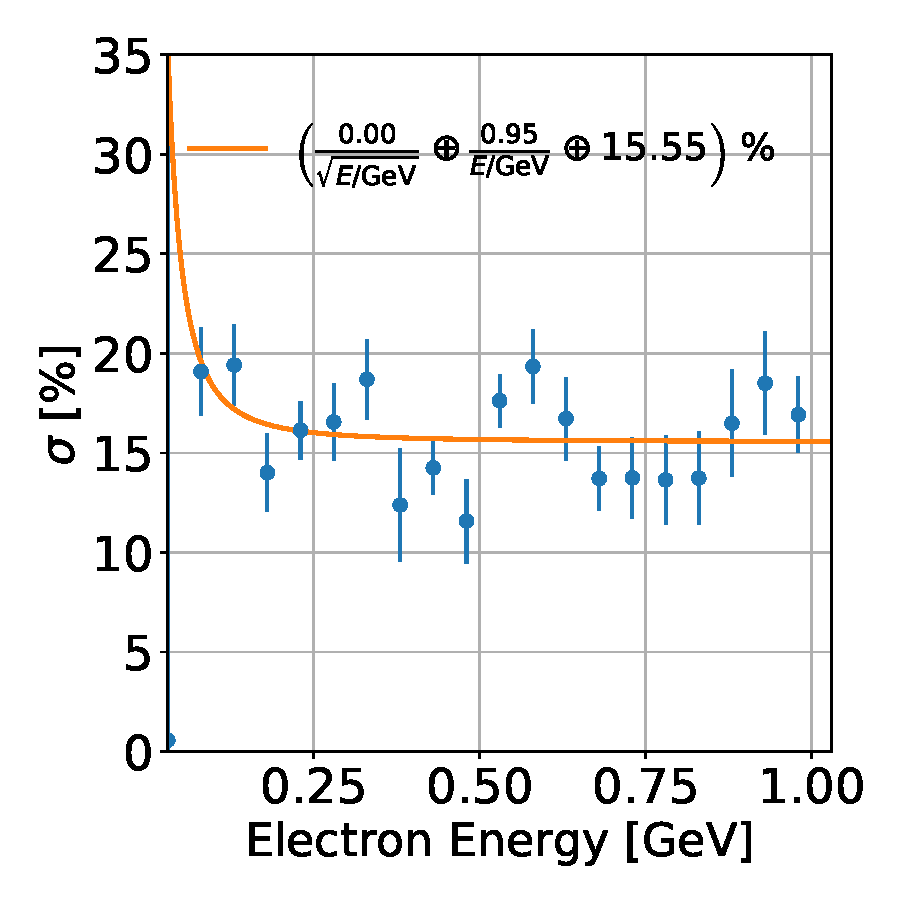
\includegraphics[width=1.00\textwidth]{ereco/elec_eres_vs_true.pdf}
    %\caption{\label{fig:eres:elec:vstrue} }
    \end{subfigure}
    \begin{subfigure}[b]{0.4\textwidth}
    \centering
    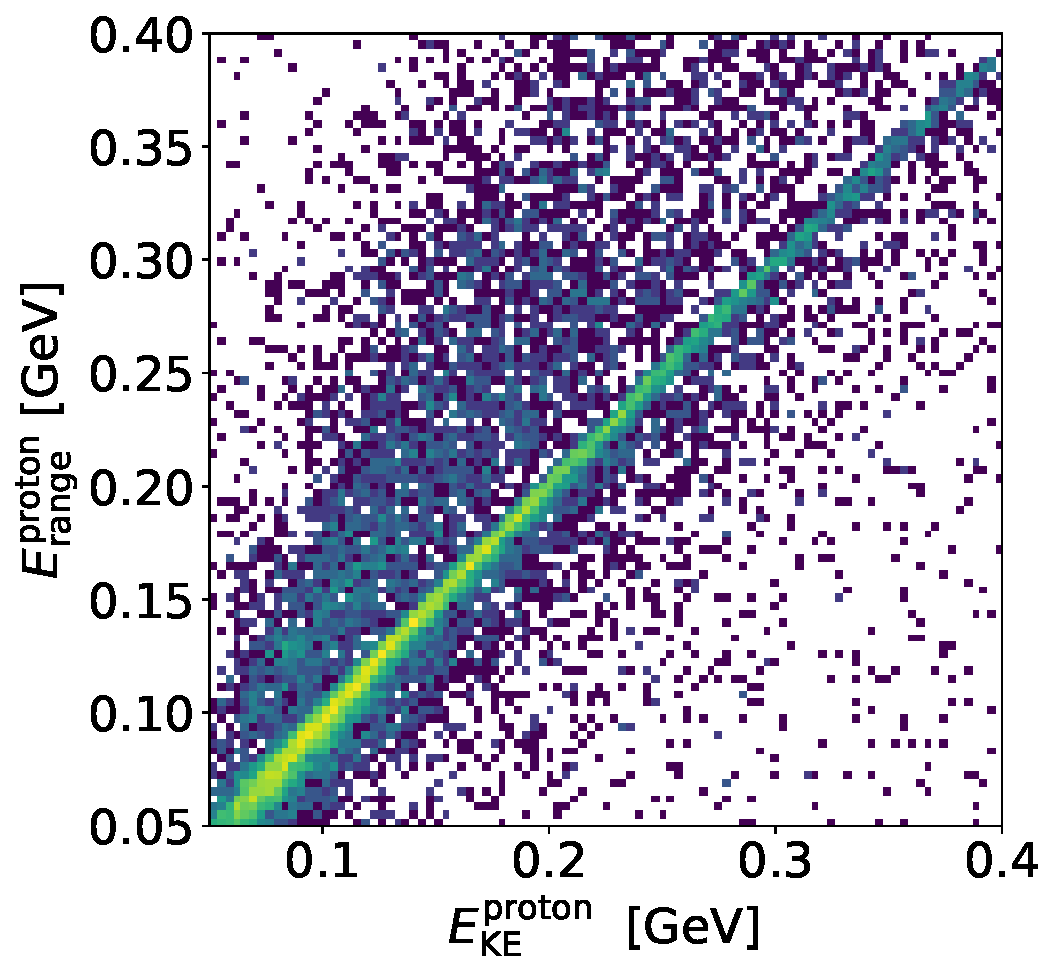
\includegraphics[width=1.00\textwidth]{ereco/proton_eres2D.pdf}
    %\caption{\label{fig:eres:proton:2d} }
    \end{subfigure}
    \begin{subfigure}[b]{0.38\textwidth}
    \centering
    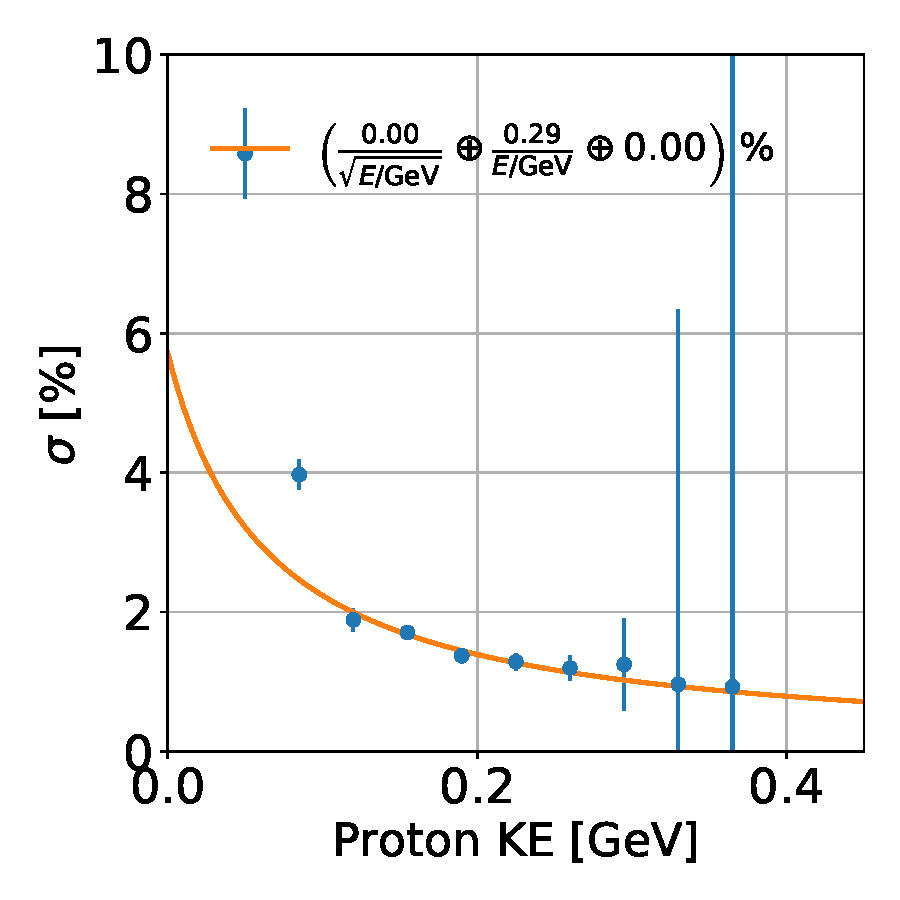
\includegraphics[width=1.00\textwidth]{ereco/proton_eres_vs_true.pdf}
    %\caption{\label{fig:eres:proton:vstrue} }
    \end{subfigure}
    \begin{subfigure}[b]{0.4\textwidth}
    \centering
    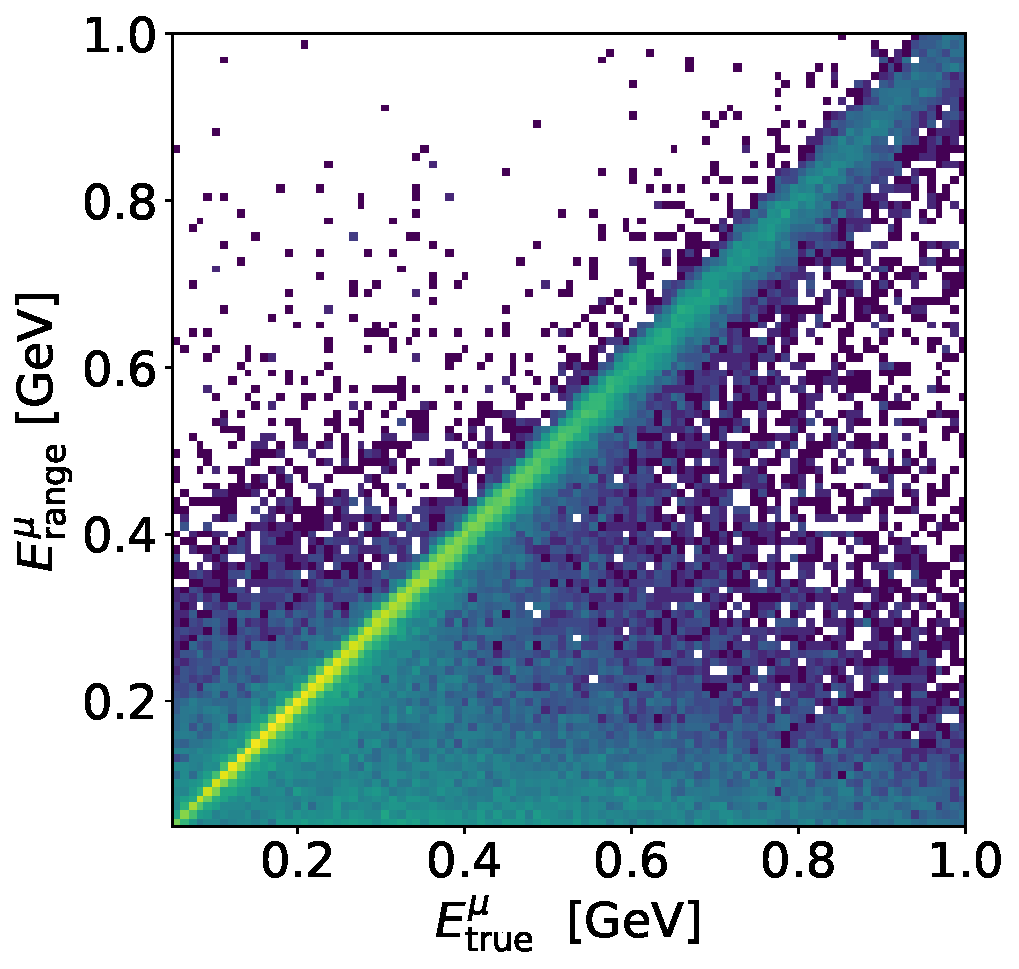
\includegraphics[width=1.00\textwidth]{ereco/muon_range_eres2D.pdf}
    %\caption{\label{fig:eres:muon:2d} }
    \end{subfigure}
    \begin{subfigure}[b]{0.38\textwidth}
    \centering
    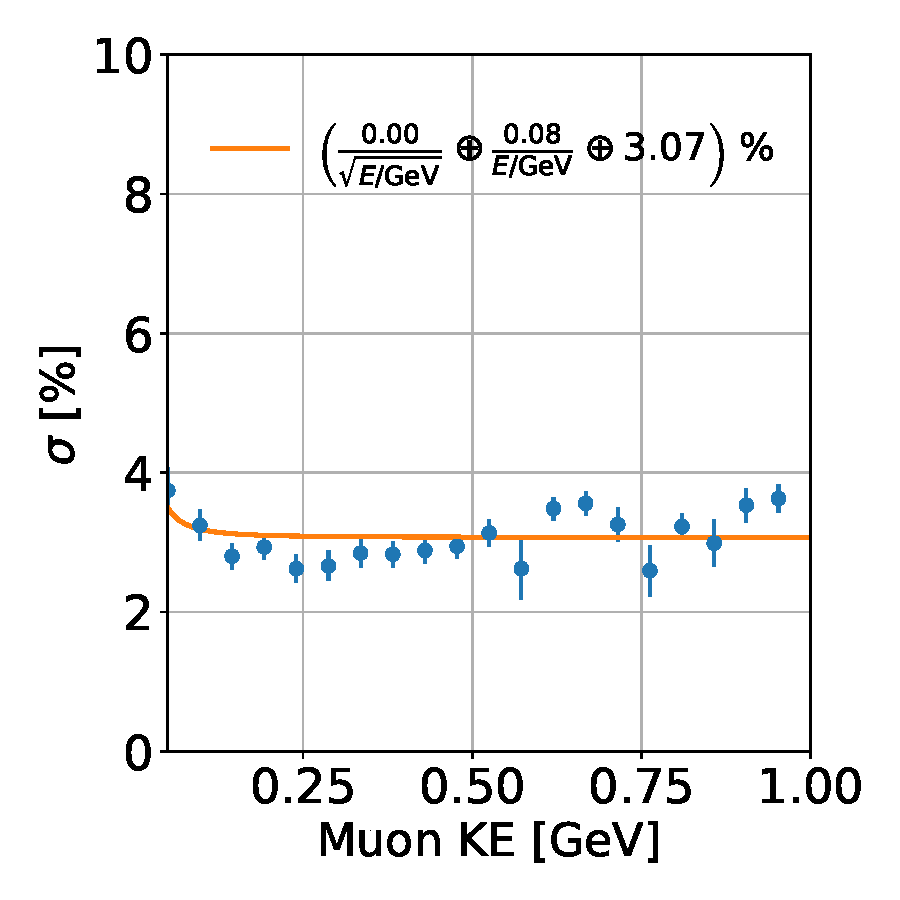
\includegraphics[width=1.00\textwidth]{ereco/muon_range_eres_vs_true.pdf}
    %\caption{\label{fig:eres:muon:vstrue} }
    \end{subfigure}
\caption{\label{fig:eres:particle}Energy resolution for electrons (top), protons (center) and muons (bottom). Left: reconstructed vs. true energy resolution (log-scale). Right: energy resolution from Gaussian fit to $[E_{\rm reco}-E_{\rm true}] / E_{\rm true}$.}
\end{center}
\end{figure}

\subsubsection{Neutrino Energy Reconstruction \textcolor{green}{Giuseppe + David, P.R. Elena}}

\par In this analysis, the energy reconstruction for neutrino interactions is performed through a sum of the visible energy of the various reconstructed final-state particles in the interaction. For $\nu_e$ events, the reconstructed energy is defined as:
\begin{equation}
    E_{\rm reco}^{\nu_e} = E_{\rm corrected}^{\rm electron} + \sum_{\rm tracks} E_{\rm range}^{\rm proton}.
\end{equation}{}
\textcolor{blue}{is this true also for nue inclusive?}.
For contained $\nu_{\mu}$ interactions, the reconstructed energy is defined as:

\begin{equation}
    E_{\rm reco}^{\nu_{\mu}} = E_{\rm range}^{\rm muon} + \sum_{\rm protons} E_{\rm range}^{\rm proton} + 0.105 \; GeV
\end{equation}{}

Figure~\ref{fig:eres:neutrino} shows the comparison between reconstructed energy and truth visible energy, which is defined as the sum of the lepton energy, pion energy (if present), and proton energy (for all protons above 40 MeV of KE). This comparison shows very accurate energy reconstruction for $\nu_{\mu}$ events \textcolor{blue}{uhm.... this is true up to a point: there's a tail for high numu visible and log numu range: does this come from events w/ non-contained muons?}. For $\nu_e$ interactions, with smearing dominated by the worse energy resolution of electron showers \textcolor{blue}{This sentence misses a verb}.

\begin{figure}[H] 
\begin{center}
    \begin{subfigure}[b]{0.4\textwidth}
    \centering
    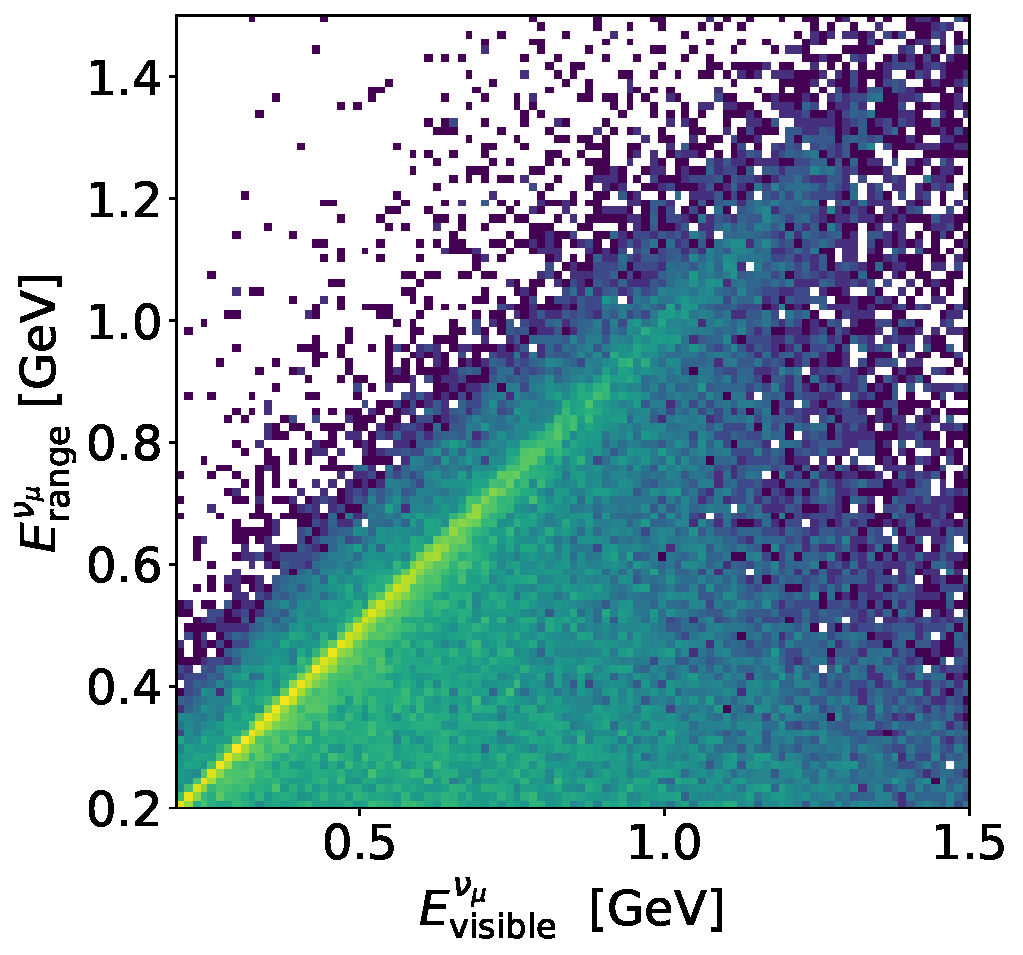
\includegraphics[width=1.00\textwidth]{ereco/numu_energy_visible_eres2D.pdf}
    \caption{\label{fig:eres:numu:2d} }
    \end{subfigure}
    \begin{subfigure}[b]{0.4\textwidth}
    \centering
    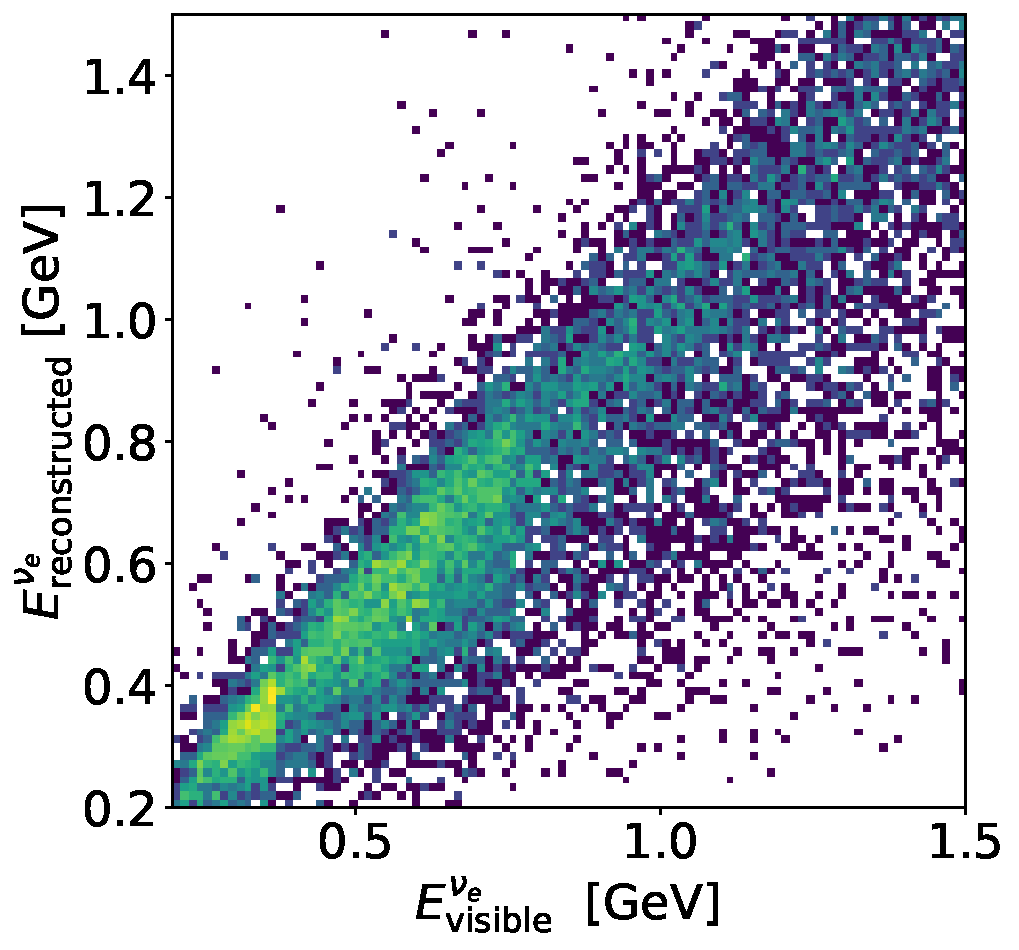
\includegraphics[width=1.00\textwidth]{ereco/nue_visible_eres2D.pdf}
    \caption{\label{fig:eres:nue:vstrue} }
    \end{subfigure}
\caption{\label{fig:eres:neutrino}Log-scale color-maps.}
\end{center}
\end{figure}

\newpage

\section{$\pi^0$ / \numu Sideband Studies}
\label{sec:controls}

\par The selections of this analysis rely on well understood detector, simulation, calibration, and analysis tools performance. This section is dedicated to evaluating the performance of detector modeling through data-mc comparisons of targeted samples. Detailed results from the $\nu_e$ low-PID and high-energy sidebands are described in section~\ref{sec:sidebands}. This chapter focuses on modeling of detector variables through the study of EM showers from $\pi^0$ decay and protons from $\nu_{\mu}$ CC interactions, as well as the modeling of $\pi^0$ production in MicroBooNE data.


\par The selections and analysis described below rely on well understood detector, simulation, calibration, and analysis tools performance. This section is dedicated to evaluating the performance of detector modeling through data-mc comparisons of targeted samples. The sidebands developed for this analysis are a high-stats $\pi^0$ selection, and an \emph{anti-BDT} filter which targets the selection of $\nu_e$ like backgrounds. \emph{Currently comparisons for the \emph{anti-BDT} filter are not available and will be documented in a future iteration of this note.}
\par It is important to note that in addition to detector simulation and reconstruction effects, $\nu$-Ar modeling can impact the level of data-mc agreement in various variables. We will try to point out when this might be the case.
\subsection{$\pi^0$ control sample}
\label{sec:controls:pi0}
\par A $\pi^0$ selection has been developed in order to obtain high-stats samples of $\pi^0$ events and $\gamma$ EM showers which can constrain $\pi^0$ production modeling uncertainties as well as validate the analyis' ability to reconstruct and select EM showers.
\par Figure~\ref{fig:pi0:mass} shows the reconstructed di-photon mass (\texttt{M$\gamma\gamma$}) for candidate $\pi^0$ events, with a calibrated but uncorrected \footnote{With the term ``uncorrected", we mean that we do not account for biases in shower energy reconstruction caused by the incompleteness in charge clustering.} energy reconstruction. Overall, there is good data-MC agreement in shape, apart from an apparent normalization difference. To account for this normalization difference, we measure the flat scaling factor  for CC and NC $\pi^0$ events needed to obtain  a consistent rate in data and MC: this factor is 72.4\% in Run1 and 72.7\% in Run3. We repeat the exercise applying a tighter $\pi^0$ selection enhancing the $\pi^0$ purity and obtain scaling factors of 70\% for both Run1 and Run3. While this procedure is far from rigorous, it allows us to study detector-related and specifically shower-related variables removing a large normalization difference. \emph{A more rigorous data-driven constrain of our $\pi^0$ rate, performed accounting for detector and flux systematics, and considering a broader range of $\pi^0$ modeling, will need to be performed.}

\begin{figure}[H] 
\begin{center}
    \begin{subfigure}[b]{0.3\textwidth}
    \centering
    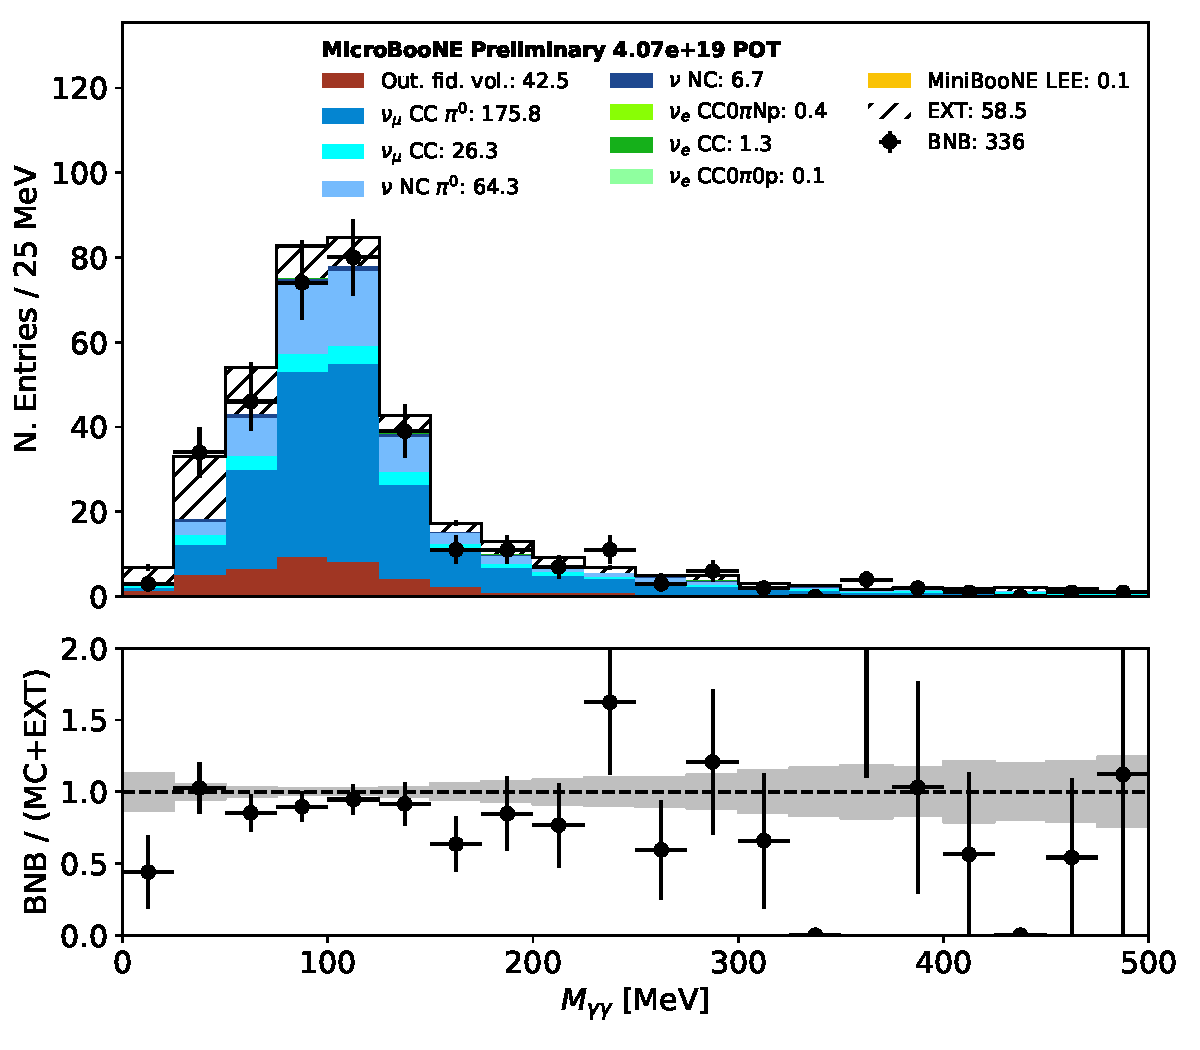
\includegraphics[width=1.00\textwidth]{pi0/pi0_mass_Y_01142020_5E19.pdf}
    \caption{\label{fig:pi0:mass:5E19} Run 1 ``5E19'' open dataset.}
    \end{subfigure}
    \begin{subfigure}[b]{0.3\textwidth}
    \centering
    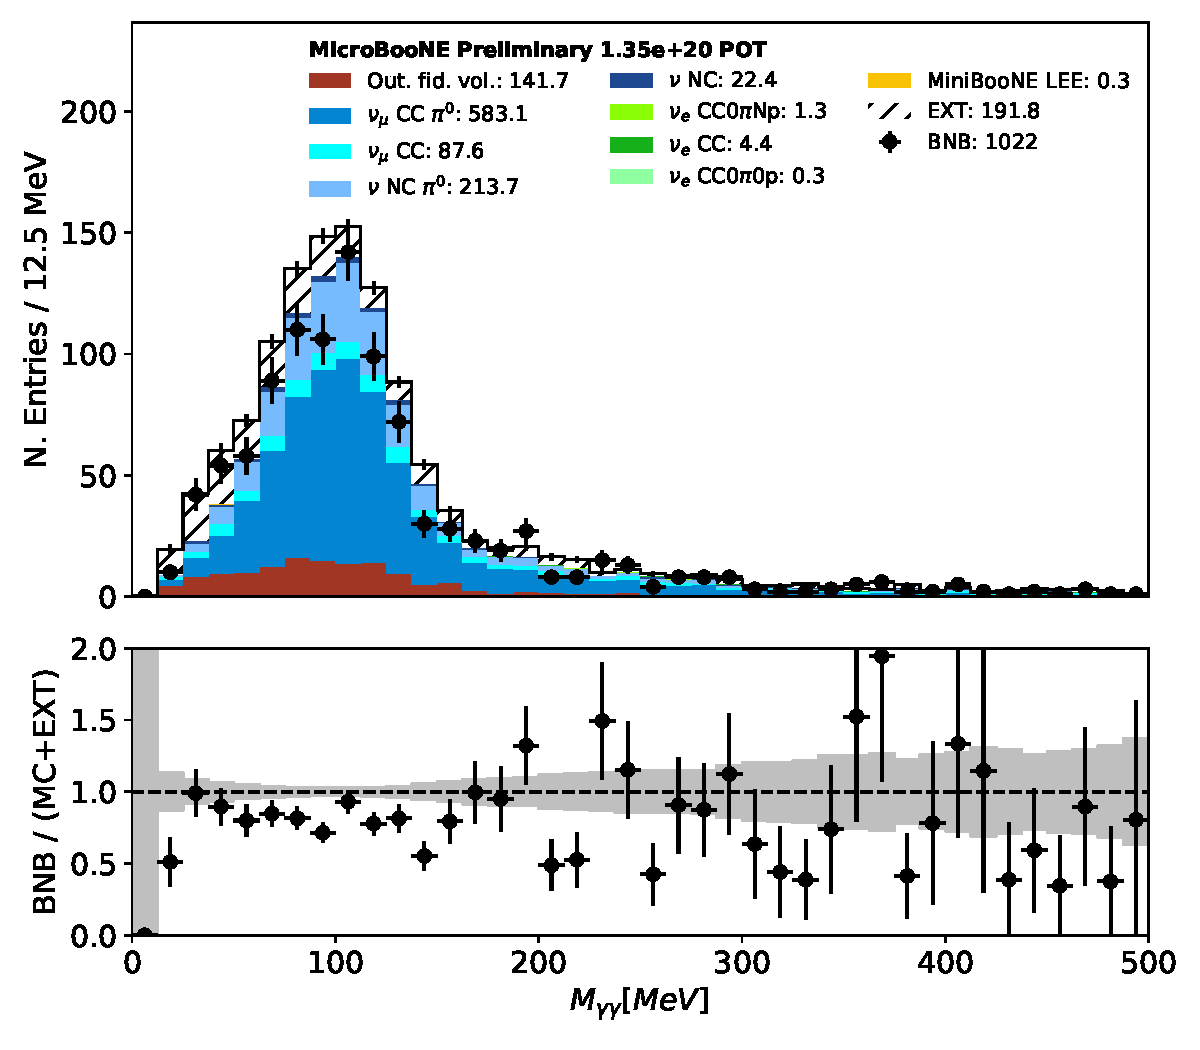
\includegraphics[width=1.00\textwidth]{pi0/pi0_mass_Y_01142020sel__RUN1.pdf}
    \caption{\label{fig:pi0:mass:5E19} Run 1.}
    \end{subfigure}
    \begin{subfigure}[b]{0.3\textwidth}
    \centering
    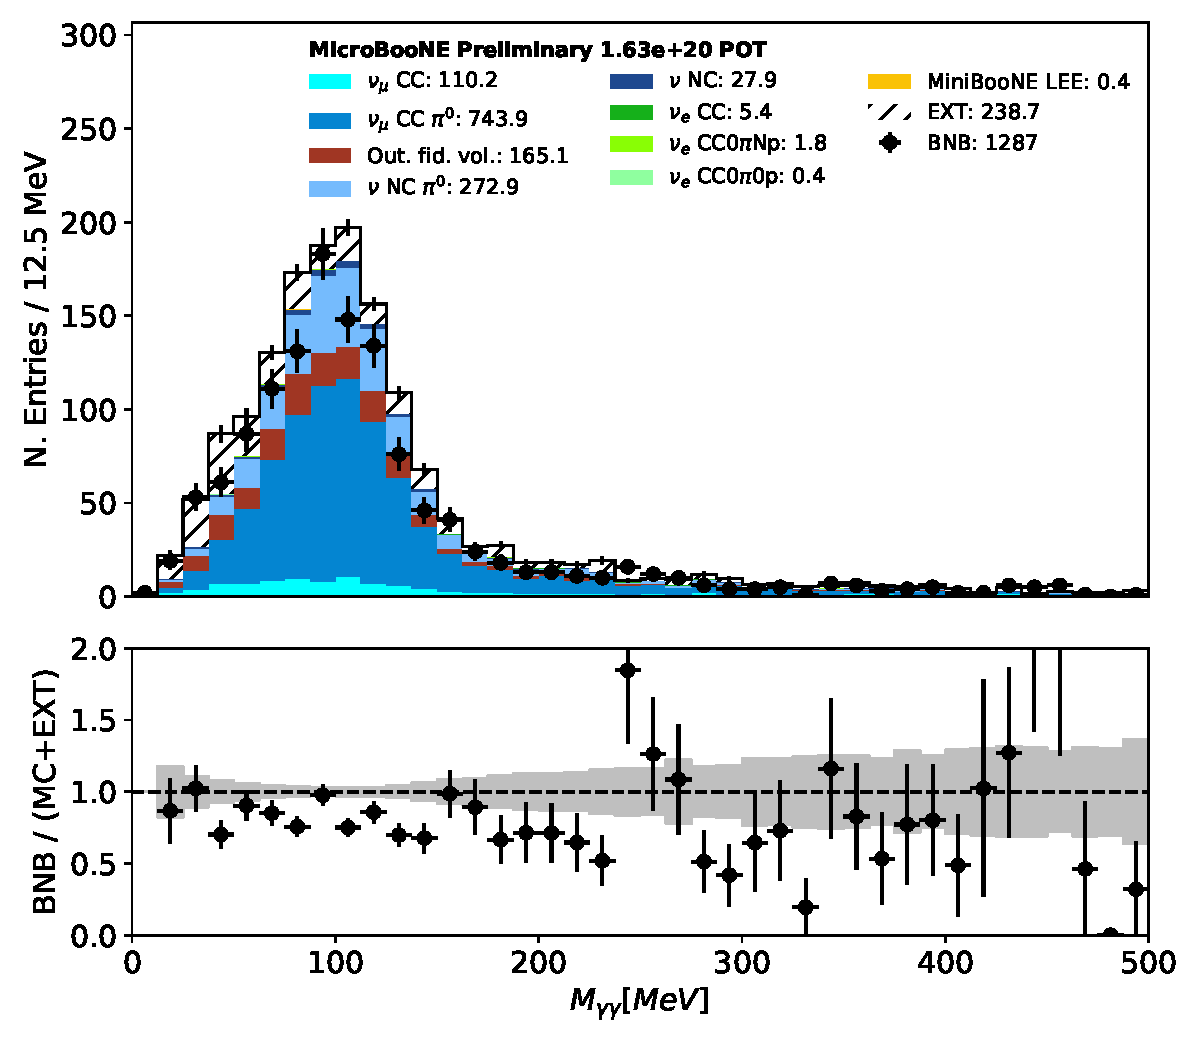
\includegraphics[width=1.00\textwidth]{pi0/pi0_mass_Y_01142020sel_RUN3.pdf}
    \caption{\label{fig:pi0:mass:5E19} Run 3.}
    \end{subfigure}
\caption{\label{fig:pi0:mass}Reconstructed $\pi^0$ mass.}
\end{center}
\end{figure}

\par After applying a scaling factor of 0.7 to CC and NC $\pi^0$ events in the MC, we show comparisons of shower variables with the goal of assessing data-mc agreement for the $\nu_e$ selection. Figure~\ref{fig:pi0:datamc} shows reconstructed quantities used in the $\nu_e$ analysis for $\pi^0$ candidate events which are useful in validating the robustness of shower modeling. They include leading and sub-leading shower dE/dx (top), followed by the leading and sub-leading shower conversion distance and shower score. The last row reports the reconstructed shower Moliere angle and track PID score for the longest track in each event. Generally, the data-MC agreement is quite good. For d$E$/d$x$ there appears to be a one bin shift to the left in data, specifically in the 4 MeV/cm peak associated with photons (see figure~\ref{fig:pi0:datamc} top-left). \emph{A re-calibration of shower d$E$/d$x$ is planned for the analysis, but has not been fully implemented at the moment.}

\begin{figure}[H] 
\begin{center}
    \begin{subfigure}[b]{0.38\textwidth}
    \centering
    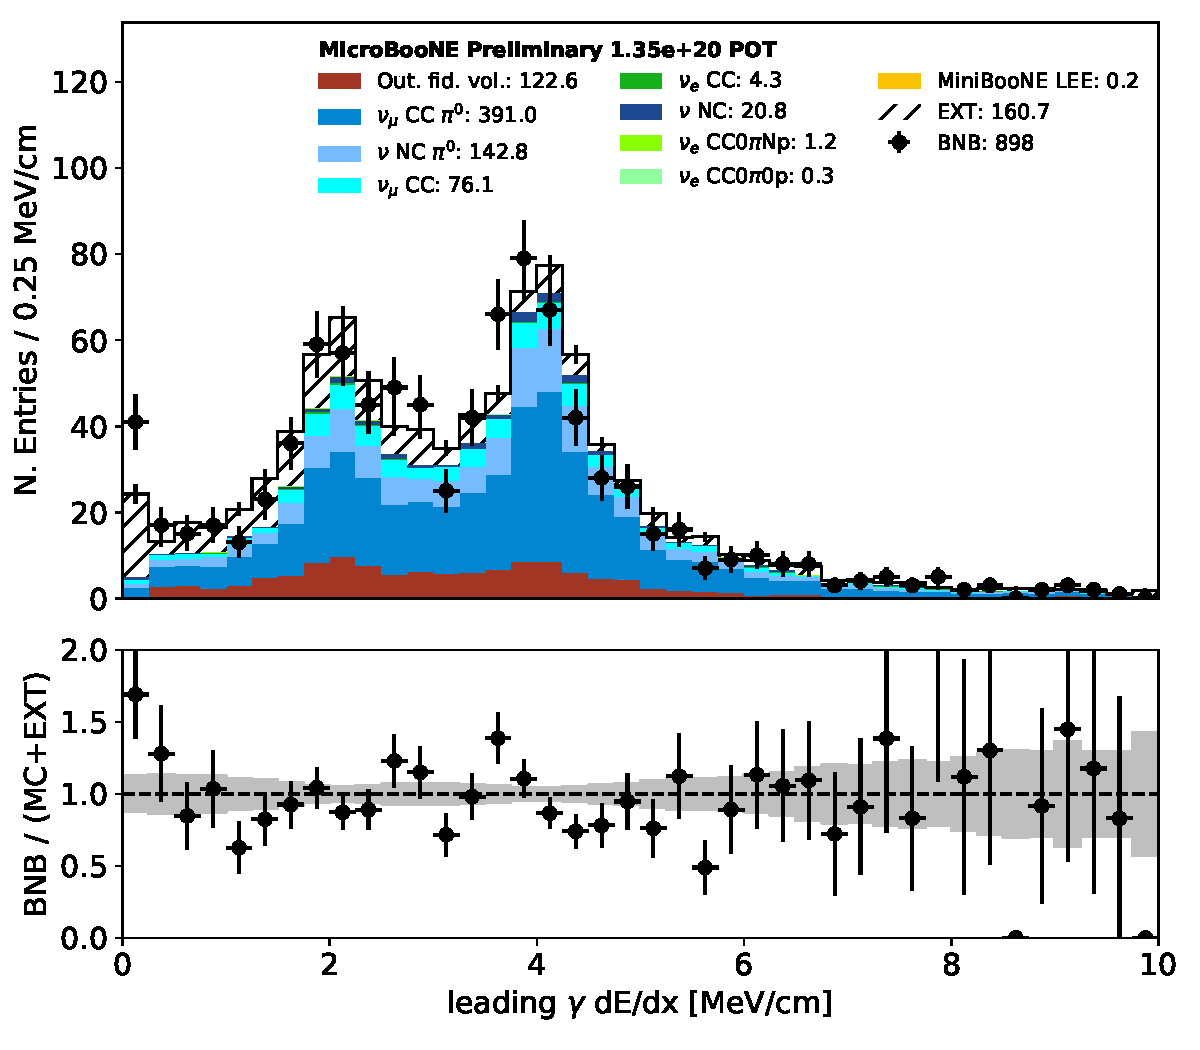
\includegraphics[width=1.00\textwidth]{pi0/pi0_dedx1_fit_Y_01152020_scaled_RUN1.pdf}
    %\caption{\label{fig:pi0:dedx:RUN1:leading} Run 1 leading shower.}
    \end{subfigure}
    \begin{subfigure}[b]{0.38\textwidth}
    \centering
    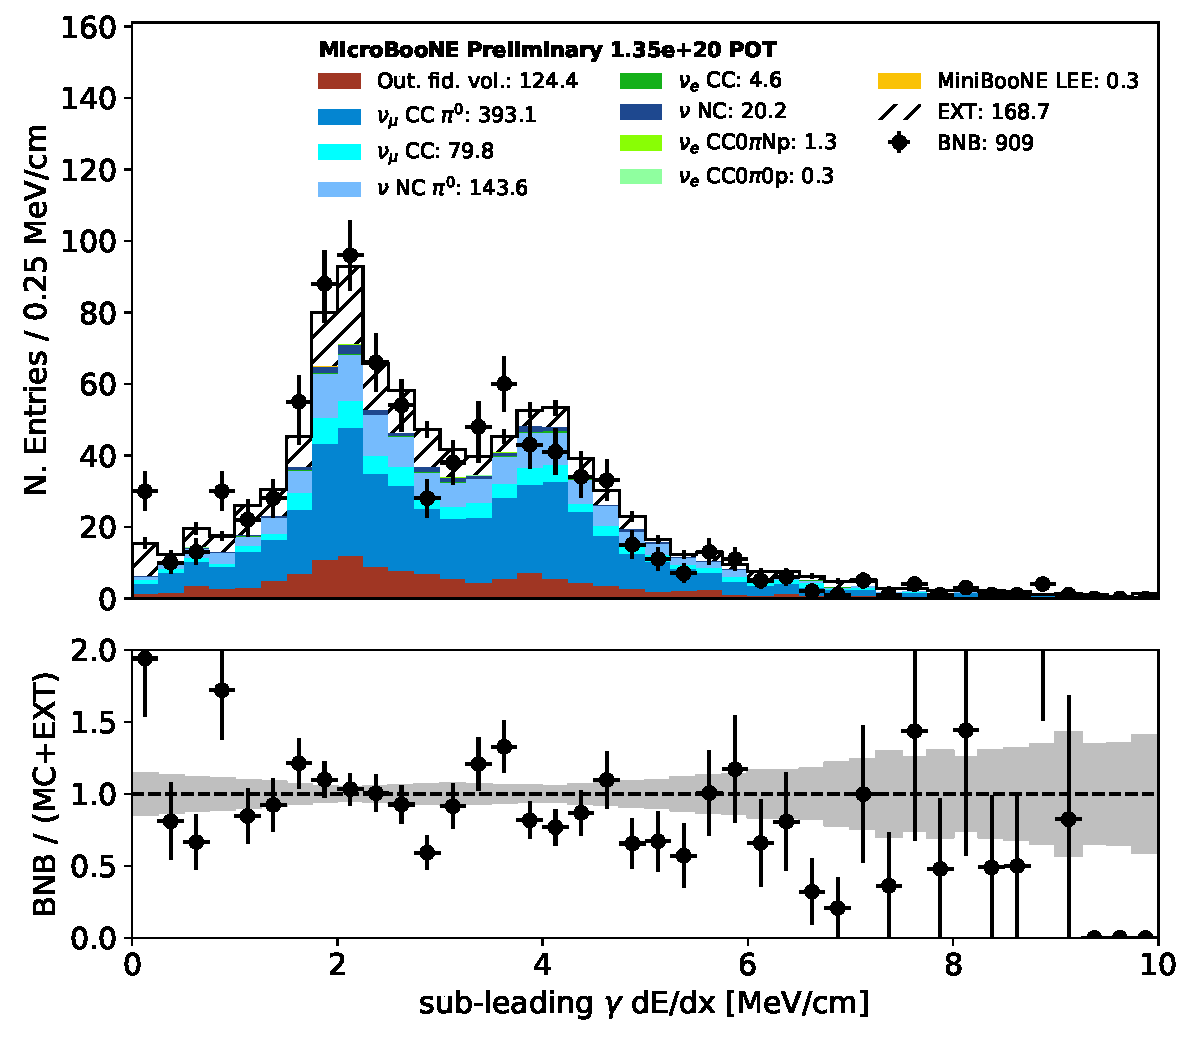
\includegraphics[width=1.00\textwidth]{pi0/pi0_dedx2_fit_Y_01152020_scaled_RUN1.pdf}
    %\caption{\label{fig:pi0:dedx:RUN1:subleading} Run 1 sub-leading shower.}
    \end{subfigure}
    
    \begin{subfigure}[b]{0.38\textwidth}
    \centering
    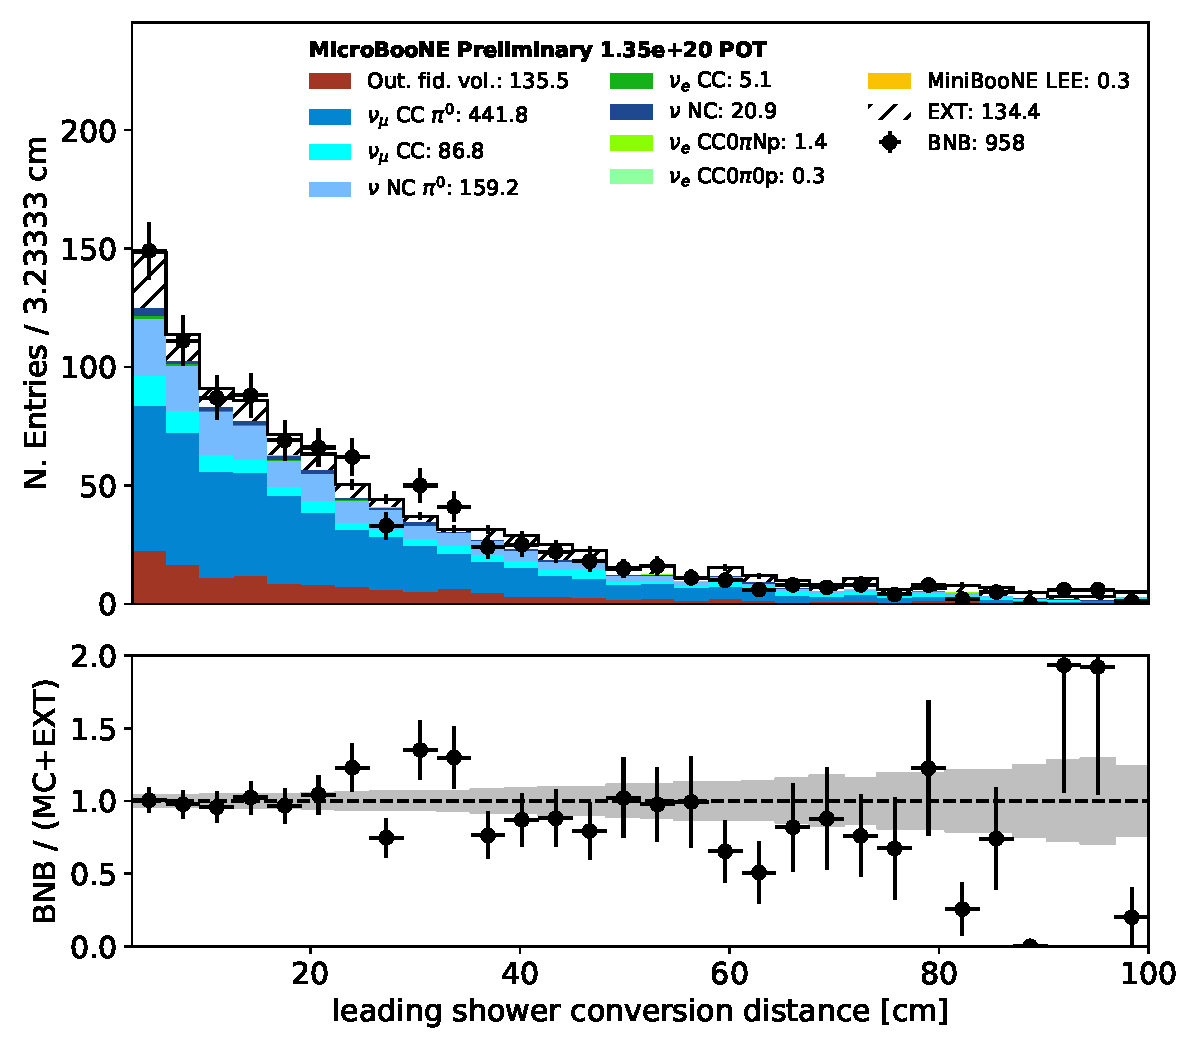
\includegraphics[width=1.00\textwidth]{pi0/pi0_radlen1_01152020_inputs_RUN1.pdf}
    %\caption{\label{fig:pi0:dedx:RUN1:leading} Run 1 leading shower.}
    \end{subfigure}
    \begin{subfigure}[b]{0.38\textwidth}
    \centering
    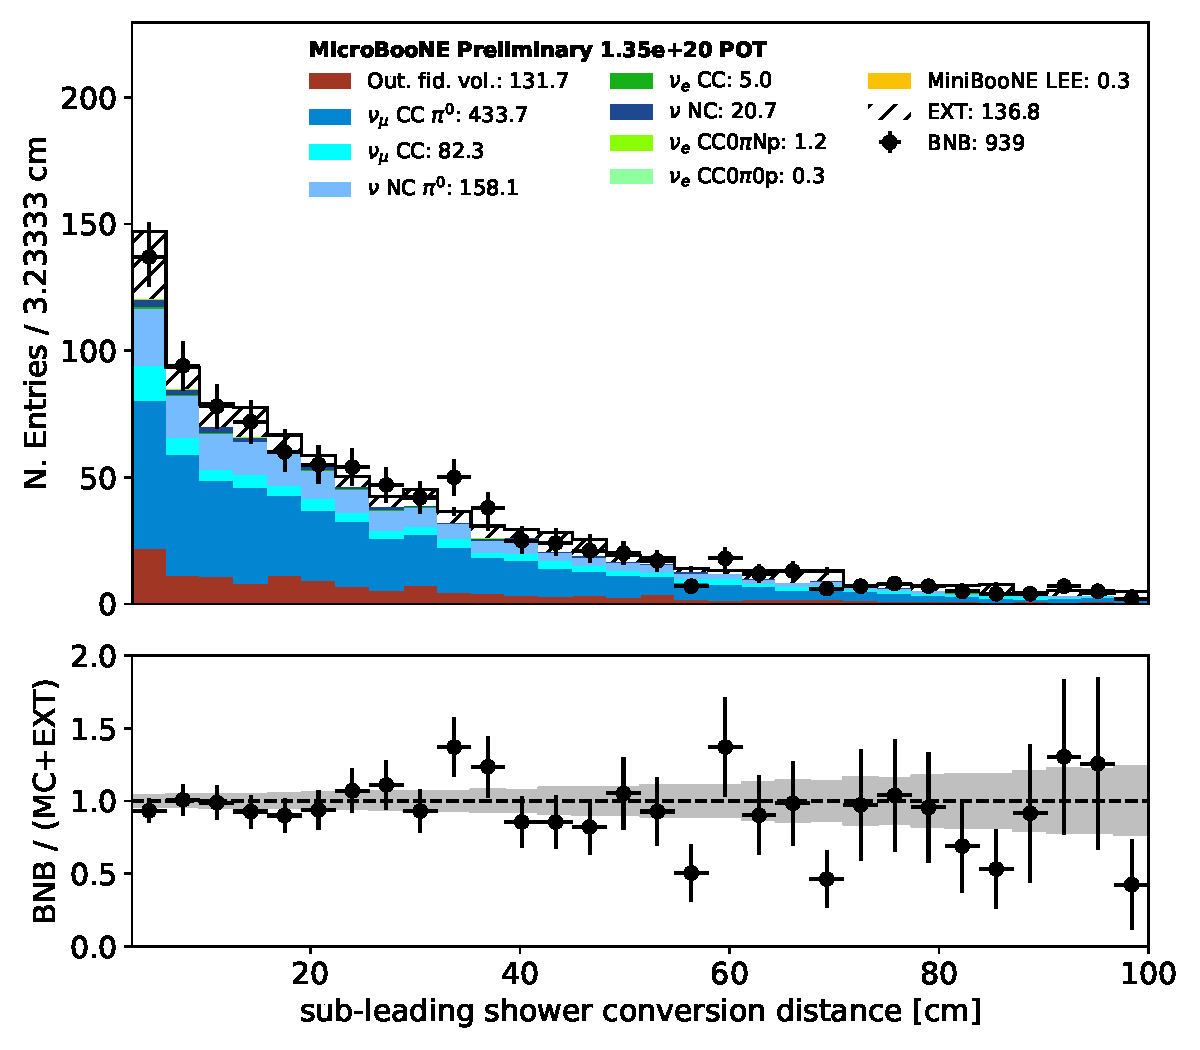
\includegraphics[width=1.00\textwidth]{pi0/pi0_radlen2_01152020_inputs_RUN1.pdf}
    %\caption{\label{fig:pi0:dedx:RUN1:subleading} Run 1 sub-leading shower.}
    \end{subfigure}
    
    \begin{subfigure}[b]{0.38\textwidth}
    \centering
    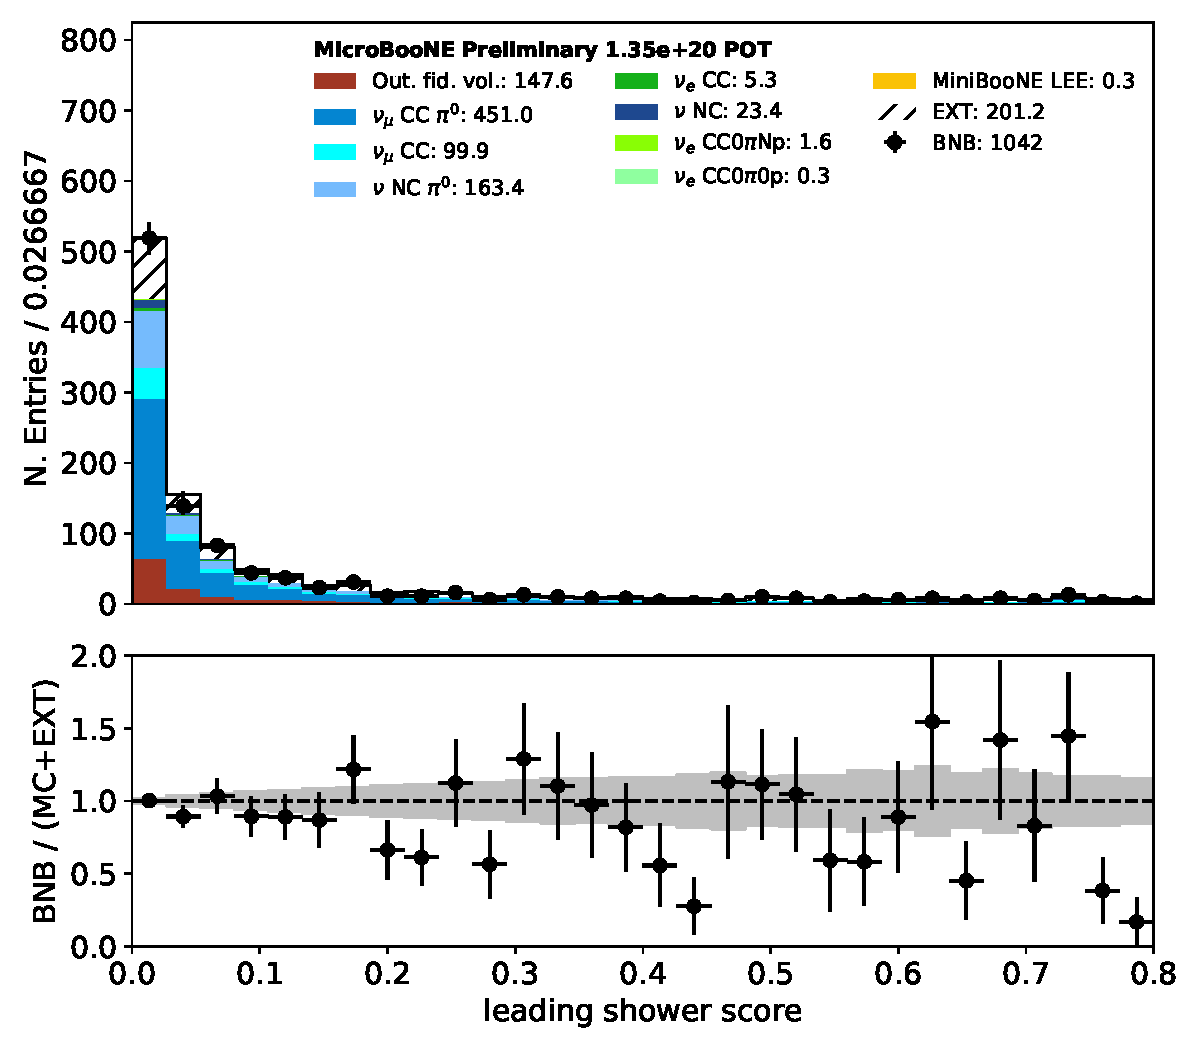
\includegraphics[width=1.00\textwidth]{pi0/pi0_shrscore1_01152020_inputs_RUN1.pdf}
    %\caption{\label{fig:pi0:dedx:RUN1:leading} Run 1 leading shower.}
    \end{subfigure}
    \begin{subfigure}[b]{0.38\textwidth}
    \centering
    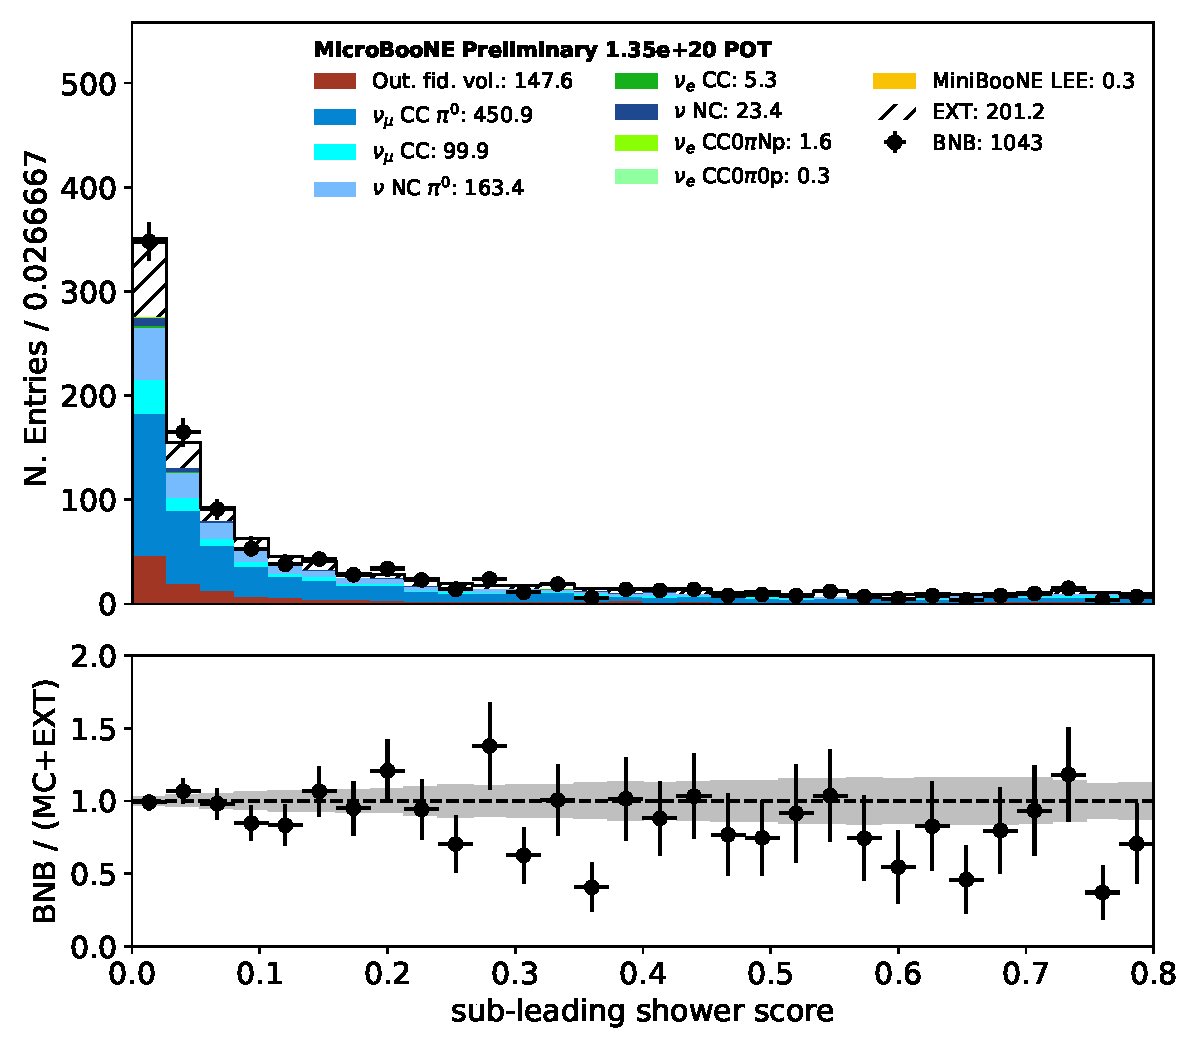
\includegraphics[width=1.00\textwidth]{pi0/pi0_shrscore2_01152020_inputs_RUN1.pdf}
    %\caption{\label{fig:pi0:dedx:RUN1:subleading} Run 1 sub-leading shower.}
    \end{subfigure}
    
    \begin{subfigure}[b]{0.38\textwidth}
    \centering
    \includegraphics[width=1.00\textwidth]{pi0/shrmoliereavg_01152020_scaled_RUN3.pdf}
    %\caption{\label{fig:pi0:dedx:RUN1:leading} Run 1 leading shower.}
    \end{subfigure}
    \begin{subfigure}[b]{0.38\textwidth}
    \centering
    \includegraphics[width=1.00\textwidth]{pi0/trkpid_01152020_scaled_RUN3.pdf}
    %\caption{\label{fig:pi0:dedx:RUN1:subleading} Run 1 sub-leading shower.}
    \end{subfigure}
    
\caption{\label{fig:pi0:datamc}Reconstructed d$E$/d$x$ for leading and sub-leading showers.}
\end{center}
\end{figure}

\subsection{Anti-BDT sample}
\par An anti-BDT filter was developed with the goal of isolating $\nu_e$ like backgrounds that could help study in detail data-mc agreement for events that are close to, but not in the $\nu_e$ signal region. The filter selects events that pass the $\nu_e$  pre-selection but fail a past iteration of the 1$e$N$p$ BDT, in order to veto and remain blind to signal events. The filter was run on $1.5E20$ POT of Run 3 data with the goal of studying in particular detail data-mc agreement for Run3, which otherwise would be limited to $0.8E19$ POT of open data. Further documentation on the \emph{anti-BDT} filter is available in reference~\cite{bib:antiBDT}. \emph{Comparisons of distributions from this filter are to be made available in a subsequent version of this note.}

\newpage



\section{$\nu_e$ Exclusive Selections}
\label{sec:nueselection}
\par This section presents the two exclusive $\nu_e$ selections which are used in the low-energy analysis. We start with describing the common variables and tools leveraged by all $\nu_e$ selections in section~\ref{sec:nueselection:variables}. Next, the \npsel (sec.~\ref{sec:nueselection:1eNp}) and \zpsel (sec.~\ref{sec:nueselection:1e0p}) channel selections are presented, starting with a description of where the two selections branch off in sec.~\ref{sec:nueselection:inputs}. The $\nu_e$ inclusive selection, sensitive to a higher energy range, will be presented in a Sec.\ref{sec:nueselection:inclusive}.

\subsection{Variable definitions}
\label{sec:nueselection:variables}
\par This section describes the variables used in the $\nu_e$ selections to isolate features that are specific to events with final-state electrons. We split these variables in several categories according to the pertinence of the calorimetric or topological information used: Slice Variables, Shower, Track, Shower and Track, and Shower/Track-like  Classification Variables,  2nd Shower-Based $\pi^0$ Rejection Variables.  While table ~\ref{tab:variableSummary} summarizes all variables used with a brief description, variables that warrant a longer introduction are described below.

\par \noindent  \textbf{Slice Variables}: these variables describe general features of the reconstructed neutrino interaction or event.
\par \noindent  \textbf{Track Variables}: these variables describe the features of tracks objects.
\par \noindent \textbf{Shower Variables}:  these variables describe the features of shower objects.
\par \noindent \textbf{Shower-Track Distance Variables}: these variables are used to measure the separation in space between the leading shower and the leading track, for events where at least one track and one shower are present in the slice. 
\begin{itemize}
 \item[] \textbf{3D shower-track distance} (variable: \emph{tksh\_distance}).  This variable is the 3D distance between the shower start point and the reconstructed start point of the longest track in the slice. 
 \item[] \textbf{2D track-shower distance} (variable: \emph{trkshrhitdist2}) Due to mis-reconstruction in the 3D shower and track reconstruction, sometimes the 3D distance just defined (\emph{tksh\_distance}) is significantly smeared (up to several centimeters) even if the individual track and shower are correctly clustered. These factors decreases the track-shower separation of $\nu_e$ interactions therefore reducing the $e-\gamma$ separation power achievable. To overcome this failure specific to the 3D reconstruction, a new quantity is calculated with 2D information from the collection plane defined as the smallest 2D distance between any hits associated with the shower candidate and any hits associated with the proton candidate. This variable is therefore complementary to the quantity \emph{tksh\_distance}.
\end{itemize}



\par \noindent \textbf{Shower/Track-like  Classification Variables}: The first step in track-shower classification relies on the topological score reconstructed by Pandora (variable: \emph{shr\_score}), which utilizes inputs such as the PCA component of 3D space-points to classify PFParticles. Nonetheless, this classification is not sufficient to obtain the track-shower separation needed. To improve on this, additional variables which leverage different aspects of shower topologies are devised:

\begin{itemize}

    \item[] \textbf{Shower Track-Fitted Fraction} (variable: \emph{trfit}, figure~\ref{fig:nue:variables:trkfit}) This quantity is the fraction of the 3D spacepoints in a shower object that are successfully fit with the shower track-fitter algorithm. Tracks, comprised of a single contiguous segment, will be entirely fit, leading to a fraction of 1. Showers, with several branches and split charge deposition segments, will have a fraction that is less then one.
    \item[] \textbf{Shower Sub-Clusters} (variable: \emph{subcluster}, figure~\ref{fig:nue:variables:subcluster}) This quantity leverages the fact that EM showers are often comprised of several branches isolated by gaps caused by photons propagating through the detector medium. The variable is calculated by counting the number of isolated 2D segments of charge associated to reconstructed showers. This quantity is a sum of such clusters from all three planes.
    \item[] \textbf{Moliere ``Angle''} (variable: \emph{shrmoliereavg}, figure~\ref{fig:nue:variables:dedx}) This quantity aims to characterize the profile of reconstructed EM showers. It is computed using 3D spacepoints. For each 3D spacepoint, the angle between the shower's direction and the spacepoint is calculated. The average of all such angles is used as the variable.
    \item[] \textbf{dE/dx Variables} (variables: \emph{shr\_tkfit\_2cm\_dedx\_\{U,V,Y\}} and \emph{shr\_tkfit\_gap10\_dedx\_\{U,V,Y\}} )  These variables are computed using calorimetric information from each plane separately. The two different variables are calculated as the median d$E$/d$x$ computed over some segment of a shower's trunk. The two segments used are the first two centimeters, and the range [1,5] cm, respectively. Two reasons justify the us of both these variables. Firstly, there are cases where the first few hits of a shower merge activity from short protons, causing a large d$E$/d$x$ which hampes the ability to identify the shower as an electron. These cases are particularly relevant as backgrounds for the 1$e$0$p$ channel. Secondly, in case of photon showers, d$E$/d$x$ becomes more and more MIP-like as one moves further along the shower, especially at low energy (see figure~\ref{fig:dedxgammas:dist}).
\end{itemize}{}

\begin{figure}[H] 
\begin{center}
    \begin{subfigure}[b]{0.3\textwidth}
    \centering
    \includegraphics[width=1.00\textwidth]{nueselection/variables/trkfit.png}
    \caption{\label{fig:nue:variables:trkfit} ``trkfit'' variable }
    \end{subfigure}
    \begin{subfigure}[b]{0.3\textwidth}
    \centering
    \includegraphics[width=1.00\textwidth]{nueselection/variables/nbranch.png}
    \caption{\label{fig:nue:variables:subcluster} ``subcluster'' variable }
    \end{subfigure}
    \begin{subfigure}[b]{0.3\textwidth}
    \centering
    \includegraphics[width=1.00\textwidth]{nueselection/variables/dedx.png}
    \caption{\label{fig:nue:variables:dedx} d$E$/d$x$ variables }
    \end{subfigure}
\caption{\label{fig:nue:presel:eff} Additional shower variables defined by the analysis to improve track-shower separation.}
\end{center}
\end{figure}

\par \noindent  \textbf{Second Shower Based $\pi^0$ Rejection Variables}: %Often, one of the two EM $\gamma$ showers in $\pi^0$ events is not fully reconstructed by Pandora. In many cases, these second $\gamma$ showers are correctly identified by Pandora as belonging to the neutrino slice (reconstructed in 2D), but never fully reconstructed in 3D (see fig.~\ref{fig:nue:variables:secondshowerevd}).
Pandora's reconstruction of events containing $\pi^0$ is often imperfect. In many cases, both EM $\gamma$ showers are correctly identified as belonging to the same neutrino slice (reconstructed in 2D), but one of the showers is not fully reconstructed in 3D (see fig.~\ref{fig:nue:variables:secondshowerevd}).

To improve on our $\pi^0$ rejection, we build several variables storing information associated to the largest 2D cluster in the slice on each plane. At the moment, only collection-plane variables are used. The variables, shown graphically in figure~\ref{fig:nue:variables:secondshower}, are described in table ~\ref{tab:variableunSummary}. In the example event of figure~\ref{fig:nue:variables:secondshowerevd}, these quantities are computed for the circles black cluster of charge which represents a missed photon in the $\pi^0$ reconstruction.

\begin{figure}[H] 
\begin{center}
    \begin{subfigure}[b]{0.35\textwidth}
    \centering
    \includegraphics[width=1.00\textwidth]{nueselection/variables/secondshowerevd.png}
    \caption{\label{fig:nue:variables:secondshowerevd} unclustered shower }
    \end{subfigure}
    \begin{subfigure}[b]{0.35\textwidth}
    \centering
    \includegraphics[width=1.00\textwidth]{nueselection/variables/secondshower.png}
    \caption{\label{fig:nue:variables:secondshower}second-shower variables }
    \end{subfigure}
\caption{\label{fig:nue:variables:secondshower} Visual representation of the second shower based $\pi^0$ rejection variables. Left: example event where the second shower in a $\pi^0$ event is clustered in 2D (black hits) but not fully reconstructed in 3D. Right: reconstructed variables associated to the 2nd-shower search. The gray cone in the image represents the black cluster on the left image, for which only 2D information is accessible.}
\end{center}
\end{figure}

\begin{table}[ht]
\caption{\label{tab:variableSummary} Summary of the definition for the variables used in the analysis.}
\centering
\begin{tabular}{ m{0.08\textwidth} | m{0.25\textwidth} | m{0.6\textwidth}  }
Category & Variable Name & Description  \\
\hline

\multicolumn{1}{l|}{} & \emph{nslice} &  Number of neutrino slices identified by the \emph{SliceID}. Values are  0 or 1.\\  \cline{2-3}
\multicolumn{1}{l|}{} & \emph{reco\_nu\_vtx\_sce\_\{x,y,z\}} & Reconstructed neutrino interaction vertex in (x,y,z) coordinates. The space charged correction is applied.  \\  \cline{2-3}
\multicolumn{1}{l|}{} & \emph{n\_showers\_contained} & Number of showers with a starting point within the fiducial volume. \\  \cline{2-3}
\multicolumn{1}{l|}{} & \emph{n\_tracks\_contained} & Number of tracks fully contained in the fiducial volume.  \\  \cline{2-3}
\multicolumn{1}{l|}{} & \emph{contained\_fraction} & Hits in PFParticles contained in the fiducial volume over the total number of clustered hits in the slice.  \\  \cline{2-3}
\parbox[t]{2mm}{\multirow{4}{*}{\rotatebox[origin=c]{90}{Slice}}} & \emph{hits\_ratio} & Ratio between hits from showers and total number of hits in the slice. \\  \cline{2-3}
\multicolumn{1}{l|}{} & \emph{CosmicIP} & Closest distance between shower start and space points associated to tracks flagged as cosmics. \\  \cline{2-3}
\multicolumn{1}{l|}{} & \emph{crtveto} & Boolean variable checking if the event passes the CRT veto. \\  \cline{2-3}
\multicolumn{1}{l|}{} & \emph{\_closestNuCosmicDist} &  3D distance between the reconstructed neutrino vertex and the closest CRT-tagged cosmic track. \\  \cline{2-3}
\multicolumn{1}{l|}{} & \emph{slclustfrac} & Fraction of hits in the slice that are fully reconstructed to 3D particles. \\  \cline{2-3}
\multicolumn{1}{l|}{} & \emph{nObjHits\_\{U,V,Y\}} & Number of hits associated with the object on each plane.\\  \cline{2-3}
\hline

\hline
\multicolumn{1}{l|}{} & \emph{pfp\_generation} & The generation of the PFParticle according to Pandora: the neutrino has generation 1, it's direct daughters 2, and further decay products 3 or higher.\\  \cline{2-3}
\multicolumn{1}{l|}{} & \emph{trkpid}  &  Proton-muon LLR particle identification. \\  \cline{2-3}
\parbox[t]{2mm}{\multirow{4}{*}{\rotatebox[origin=c]{90}{Track, Shower and Their Separation}}}  & \emph{shr\_energy\_tot\_cali}  & Sum  of  the  energy  of  the  calibrated  showers  (in  GeV). Used  only  at pre-selection as a ``Michel veto”.\\  \cline{2-3}
\multicolumn{1}{l|}{} & \emph{shr\_score} & Pandora  SVM track/shower score for the leading shower.\\  \cline{2-3}
\multicolumn{1}{l|}{}  & \emph{tksh\_distance}  & Distance between leading shower and longest track start points.\\  \cline{2-3}
\multicolumn{1}{l|}{} & \emph{tksh\_angle}  & Angle  between  leading  shower   and  longest  track directions.\\  \cline{2-3}
\multicolumn{1}{l|}{} & \emph{merge\_bestdist}  & Distance between shower start point and track start (or end) point for the track in the slice that best matches the direction of the shower.\\  \cline{2-3}
\multicolumn{1}{l|}{} & \emph{trfit} & Fraction of the 3D spacepoints successfully fitted with the shower track-fitter algorithm. \\  \cline{2-3}
\multicolumn{1}{l|}{} & \emph{subcluster} & Number of isolated 2D segments of charge associated to a reconstructed shower on all three planes  \\  \cline{2-3}
\multicolumn{1}{l|}{} & \emph{shrmoliereavg} &  Average angle between the shower’s direction and its 3D spacepoints.    \\ \cline{2-3}
\multicolumn{1}{l|}{} & \emph{shr\_tkfit\_gap10\_dedx\_\{U,V,Y\}}  & Median dE/dx computed over the [1,5] cm of the shower’s  trunk. \\ \cline{2-3}
\multicolumn{1}{l|}{} & \emph{shr\_tkfit\_2cm\_dedx\_\{U,V,Y\}}  & Median dE/dx computed  over  the first 2 cm of the shower’s  trunk. \\ \cline{2-3}
\multicolumn{1}{l|}{} & \emph{shower\_vtx\_dist} & Distance between the shower start and the neutrino vertex.\\ \cline{2-3}
\multicolumn{1}{l|}{} & \emph{ismerged} & Check if a proton is merged at the beginning of a shower.\\ \cline{2-3}
\hline
\hline
\multicolumn{1}{l|}{} & \emph{secondshower\_Y\_nhit} & Number of hits in the collection plane of the largest cluster associated to the  recovered 2nd shower  \\  \cline{2-3}
\parbox[t]{2mm}{\multirow{4}{*}{\rotatebox[origin=c]{90}{Second Shower}}}  & \emph{secondshower\_Y\_dot} &  Dot product between the vector connecting the vertex to the closest hit in cluster and the charge-weighted cluster direction w.r.t. closest hit in cluster \\  \cline{2-3}
\multicolumn{1}{l|}{} & \emph{anglediff\_Y} & 2D angle difference in the collection plane between the 2nd shower and the 1st shower cluster  (cluster direction defined as charge-weighted direction of cluster w.r.t. vertex) \\ \cline{2-3}
\multicolumn{1}{l|}{} & \emph{secondshower\_Y\_vtxdist} & 2D distance from vertex for the largest 2D cluster associated to the  recovered 2nd shower in the collection plane \\
\hline
\end{tabular}
\label{tab:variableSummary}
\end{table}

\clearpage

\subsection{Input to \npsel and \zpsel selections and channel orthogonality }
\label{sec:nueselection:inputs}

The \npsel and \zpsel selections rely on a common pre-selection which requires the presence of at least one reconstructed and contained EM shower (figure~\ref{fig:nue:presel:nshower}) with reconstructed energy above 70 MeV (figure~\ref{fig:nue:presel:shrenergy}). This second cut acts as a Michel-electron veto, since the majority of events which do not pass this cut are associated with cosmic or $\nu_{\mu}$ induced $\mu \rightarrow e$ Michel electrons. 
In addition, as a containment cut we require that more than 90\% of clustered hits in the slice are associated to PFParticles that are  contained  in the fiducial volume.
The two selections are subsequently split: we require the presence of at least one fully contained track for the \npsel channel and the absence of fully contained tracks for the \zpsel channel.

\begin{figure}[H] 
\begin{center}
    \begin{subfigure}[b]{0.3\textwidth}
    \centering
    \includegraphics[width=1.00\textwidth]{nueselection/n_showers_contained_01132020_RUN1.pdf}
    \caption{\label{fig:nue:presel:nshower} Contained showers}
    \end{subfigure}
    \begin{subfigure}[b]{0.3\textwidth}
    \centering
    \includegraphics[width=1.00\textwidth]{nueselection/n_tracks_contained_01132020_RUN1.pdf}
    \caption{\label{fig:nue:presel:ntrack} Contained tracks}
    \end{subfigure}
    \begin{subfigure}[b]{0.3\textwidth}
    \centering
    \includegraphics[width=1.00\textwidth]{nueselection/shr_energy_tot_cali_01132020_RUN1.pdf}
    \caption{\label{fig:nue:presel:shrenergy} Shower energy}
    \end{subfigure}
\caption{\label{fig:nue:presel}Variables input to the common $\nu_e$ N$p$ and 0$p$ pre-selection.}
\end{center}
\end{figure}

\begin{comment}
\par The efficiencies of the 1$e$N$p$ and 1$e$0$p$ channels at the point where the selections diverge are shown in figure~\ref{fig:nue:presel:eff}. Efficiencies are presented as a function of true neutrino energy (fig.~\ref{fig:nue:presel:eff:nu}), proton KE (fig.~\ref{fig:nue:presel:eff:proton}), and electron energy (fig.~\ref{fig:nue:presel:eff:elec}). Each plot shows in black the efficiency for the common pre-selection (before requirements on protons are imposed) relative to all intrinsic $\nu_e$ events. The efficiencies for the  1$e$N$p$ and 1$e$0$p$ selections relative to true N$p$ and 0$p$ events are shown in blue and red respectively.
Shaded histograms in red and blue show the stacked truth-level distributions for N$p$ and 0$p$ events for the variables being plotted. It is important to observe that the reconstruction efficiency for 1$e$N$p$ events is significantly lower then that of 1$e$0$p$ events at this pre-selection stage. This is caused by the additional requirement of the presence of a proton-like track in the final state. The strong energy dependence for the efficiency in tagging protons is shown in figure~\ref{fig:nue:presel:eff:proton}. While requiring the presence of a final-state proton lowers the efficiency, this requirement has a significant impact on the selection's ultimate purity.

\begin{figure}[H] 
\begin{center}
    \begin{subfigure}[b]{0.3\textwidth}
    \centering
    \includegraphics[width=1.00\textwidth]{nueselection/nu_RUN1.pdf}
    \caption{\label{fig:nue:presel:eff:nu} }
    \end{subfigure}
    \begin{subfigure}[b]{0.3\textwidth}
    \centering
    \includegraphics[width=1.00\textwidth]{nueselection/proton_RUN1.pdf}
    \caption{\label{fig:nue:presel:eff:proton} }
    \end{subfigure}
    \begin{subfigure}[b]{0.3\textwidth}
    \centering
    \includegraphics[width=1.00\textwidth]{nueselection/elec_RUN1.pdf}
    \caption{\label{fig:nue:presel:eff:elec} }
    \end{subfigure}
\caption{\label{fig:nue:presel:eff} $\nu_e$ pre-selection efficiencies split by final-state topology as a function of different truth variables. }
\end{center}
\end{figure}
\end{comment}{}

\subsection{\npsel Channel}
\label{sec:nueselection:1eNp}

The \npsel channel is the most sensitive to the MiniBooNE eLEE signal as it contains a large fraction of the signal events and allows for selection requirements based both on showers and tracks. Since $\nu_e$ charge-current interactions are O(1\%) in the BNB and a large cosmic background is present, a high-purity selection is needed to achieve a sizeable signal sensitivity; the necessary trade-off is that the final signal efficiency will be low.

The section is organized as follows. We first define a set of minimal requirements (``pre-selection") to obtain a high statistics sample used to monitor the data-MC agreement of the selection variables;
the events at the pre-selection stage are dominated by cosmic and neutrino backgrounds. We then define two alternative selections, one based on a simple box-cut approach and one on boosted decision trees (BDT); the BDT approach is expected to be the most sensitive, while box-cuts provide a robust reference selection. Finally, we compare all presented selections in terms for their signal efficiency and purity.

Two updates to the selection have been included since opening the far-sideband data for this analysis. They consist of a series of ``recovery'' algorithms which aim to re-interpret event information for events that fail the selection due to mis-reconstruction, as well as two cut updates at pre-selection stage. The recovery algorithms aim to mitigate reconstruction failures which occur largely at high-energy and do not impact the analysis at low energy. The most common such failure is associated to events where the electron is split in two reconstructed showers, which are recovered through a re-interpretation of the event as a one-shower topology. These algorithms are described in detail in sec.~\ref{sec:sideband:recovery}. The two minor cut updates, which also have no noticeable impact at low energy, are described in sec.~\ref{sec:sideband:newcuts:shrtrklen}
 and~\ref{sec:sideband:newcuts:nhits}. The contents of this chapter inclue and reflect these updates.
 
\subsubsection{Preselection}

We define a \npsel preselection by adding a requirement of at least one contained track on top of the common \nue preselection defined in Sec.~\ref{sec:nueselection}. 
The \npsel preselection is a minimum set of cuts that guarantees that all selection variables can be defined; the list of requirements can be found in Table~\ref{tab:1eNp:presel}.

\begin{table}[h!]
\centering
\setlength{\tabcolsep}{10pt}
\renewcommand{\arraystretch}{1.25}
 \begin{tabular}{| c | c |} 
 \hline
 Cut goal & Cut definition \\
 \hline\hline
Cosmic rejection & nslice = 1 \\
 \hline
\multirow{2}{*}{Signal~topology} & n\_tracks\_contained $>$ 0 \\
 & n\_showers\_contained $>$ 0 \\
 \hline
Containment & contained\_fraction $>$ 0.9 \\
 \hline
Michel rejection & shr\_energy\_tot\_cali $>$ 0.07 GeV \\
 \hline
 \end{tabular}
 \caption{\label{tab:1eNp:presel} Preselection requirements for the \npsel selection.}
\end{table}

The relative fraction of EXT events at this stage is roughly 25\%, so we can look at all selection variables in data and MC in a neutrino-dominated sample with the open Run1 and Run3 data sets. We typically see very good agreement, which rules out major problems related to POT-scaling, detector modeling, and flux and cross-section modeling. 
%The reader should keep in mind that current data-mc comparisons do not include a rescaling of the $\pi^0$ normalization, and that resolving discrepancies in $\pi^0$ normalization described in section~\ref{sec:sideband:pi0} will impact the final level of data-mc agreement. 
The full list of plots can be found in Appendix~\ref{app:nuepresel}. Figure~\ref{fig:1eNp:prsel} shows the level of agreement for the reconstructed neutrino energy variable after pre-selection. 

\begin{figure}[ht]
\begin{center}
% p-values: reco_e 0.3105 0.9905 0.8121
\includegraphics[width=0.6\textwidth]{1eNp/reco_e_presel.pdf}
\caption{\label{fig:1eNp:prsel}Reconstructed neutrino energy after pre-selection for the \npsel channel.}
\end{center}
\end{figure}

%\begin{figure}[ht] 
%\begin{center}
%    \begin{subfigure}[b]{0.45\textwidth}
%    \centering
%    \includegraphics[width=1.00\textwidth]{1eNp/reco_e_03122020_RUN1_preselection.pdf}
%    \caption{\label{fig:1eNp:prsel:RUN1} RUN 1}
%    \end{subfigure}
%    \begin{subfigure}[b]{0.45\textwidth}
%    \centering
%    \includegraphics[width=1.00\textwidth]{1eNp/reco_e_03122020_RUN3_preselection_fixed.png}
%    \caption{\label{fig:1eNp:prsel:RUN1} RUN 3}
%    \end{subfigure}
%\caption{\label{fig:1eNp:prsel}Reconstructed neutrino energy after pre-selection for the \npsel channel.}
%\end{center}
%\end{figure}


\subsubsection{\npsel Selection}

Both a box-cut and BDT-based selection have been developed for the \npsel. The BDT-based selection is expected to be the most sensitive to low-energy \nue events since BDTs are able to learn additional information from the data and return a response variable that is highly discriminating between signal and background. The box-cut selection, relying on the same input variables, can provide a robust validation of the analysis, though with lower signal sensitivity. It is documented in Appendix~\ref{app:nueslections:1eNp}. In the remainder of this section we present exclusively the BDT-based selection.

Two BDTs are trained separately to reject backgrounds with and without $\pi^0$ in the final state. The same set of training variables is used in the two BDTs, corresponding to the list of variables used in the box-cut selection. In order to avoid splitting the already limited-size samples used for the analysis, dedicated samples are used for training: the signal comes from intrinsic \nue samples in the range $0<E_\nu<400$ and $0<E_\nu<800$ \si{GeV}; EXT events are taken from a sample of about 280k events from the NuMI EXT data stream; $\pi^0$ samples for BDT training are produced recycling the EXT unbiased events used in the overlay procedure; non-$\pi^0$ neutrino-induced background samples are produced with tight filters on truth-variables that enhance $\nu_{\mu}$ 0$\pi^0$ events that contribute as backgrounds to the analysis. (\href{https://microboone-docdb.fnal.gov/cgi-bin/private/RetrieveFile?docid=28140&filename=tight-nue-back-filter-merge-memo.pdf&version=1}{DocDB 28140}). As a result the relative size of the samples varies significantly, so the event weight in training is enhanced for specific categories of backgrounds such as \numucc events with no pions or EXT and cosmic-dominated events. Training is performed after requiring \texttt{reco\_e $<$ 0.8} and \texttt{n\_showers\_contained $=$ 1} on top of the \npsel pre-selection.  

The BDT training is able to figure out which variables are most important for each background. Figure~\ref{ffig:1eNp:bdt:var} shows that, while the importance of the training variable is in general very similar in the two BDTs, there are indications that each BDT specializes for their target background; for instance, the most discriminating variable is different, being subcluster for the non-$\pi^0$ BDT and tksh\_distance for the $\pi^0$ BDT. %It is interesting to note that the most discriminating variable in both cases is shrmoliereavg, since it can be useful to discriminate both muons in $\nu_\mu$ events (low values) and merged showers in $\pi^0$ events (large values).
Validations of the BDT training variables in terms of data-MC comparison on the unbiased Run1 + Run3 5e19 datasets are presented in appendix~\ref{app:nuepresel}. Further validations of data/MC agreement from low-PID, 2+ shower, and high-energy $\nu_e$ sidebands are included in Sec.~\ref{sec:sideband:1eNp:lowpid},~\ref{sec:sideband:1eNp:2pshr}, and~\ref{sec:sideband:1eNp:he} respectively.

\begin{figure}[H] 
\begin{center}
    \begin{subfigure}[b]{0.45\textwidth}
    \centering
    \includegraphics[width=1.00\textwidth]{1eNp/bdt_var_gain.pdf}
    \caption{\label{fig:1eNp:bdt:var:gain}}
    \end{subfigure}
    \begin{subfigure}[b]{0.45\textwidth}
    \centering
    \includegraphics[width=1.00\textwidth]{1eNp/bdt_var_rank.pdf}
    \caption{\label{fig:1eNp:bdt:var:rank}}
    \end{subfigure}
\caption{\label{ffig:1eNp:bdt:var} BDT variables importance in terms of ``total gain". In \texttt{xgboost}~\cite{bib:xgboost}, "gain" is the improvement in accuracy brought by a feature to the branches it is on; "total gain" refers to the sum of the "gain" across all branches. Left: total gain value. Right: ranking based on the total gain value (highest ranking=15, lowest=1).}
\end{center}
\end{figure}

The BDT selection combines a set of loose box cuts and cuts on BDT responses. The loose box cuts are listed in Table~\ref{tab:1eNp:loosecut} and are intended to reject events where one or more variables are clearly inconsistent with \nuecc interactions. The resulting BDT responses in Run1 open data are shown in Figures~\ref{fig:1eNp:bdt:nonpi0} and \ref{fig:1eNp:bdt:pi0} for the non-$\pi^0$ and $\pi^0$ BDT, respectively. The left and right panels show the response below and above 0.5 respectively. We cut separately on the output of the two BDTs, requiring the $\pi^0$ and non-$\pi^0$ responses to be greater than 0.67 and 0.70, respectively. The cut flow table in terms of efficiency and purity at low energy is in Fig. \ref{fig:1eNp:cutflow:bdt}. The resulting reconstructed \nue energy after the BDT selection is shown in Figure~\ref{fig:1eNp:bdt:1e21}. %The (purity, efficiency) change from (0.6\%,33\%) $\righarrow$ (12\%, 12\%) $\rightarrow$ (65\%, 9\%) at pre-selection, loose box-cut, and BDT cut, respectively. The final BDT cut allows for a more than 4$\times$ increase in purity with a relative efficiency of 75\%.

Two events pass the full BDT selection in the available $4.07E19$ POT dataset from Run1. Both events appear to be good $\nu_e$ candidates (consistent with the level of purity expected), and are reconstructed with $\sim 1.1$ GeV of energy; event displays are shown in Fig.~\ref{fig:1eNp:box:evd}.

%\emph{The BDT selection can be considered final, pending more detailed checks of data-MC agreement with large statistics and the availability of additional samples for training.}

\begin{table}[h!]
\centering
\setlength{\tabcolsep}{10pt}
\renewcommand{\arraystretch}{1.25}
 \begin{tabular}{| c | c |} 
 \hline
 Cut goal & Cut definition \\
 \hline\hline
\multirow{2}{*}{Cosmic~rejection} & CosmicIPAll3D $>$ 10 \si{\cm} \\
& trkpid $<$ 0.02 \\
 \hline
\multirow{5}{*}{$\nu_\mu$~rejection} & hits\_ratio $>$ 0.5 \\
& shrmoliereavg $<$ 9\si{\degree} \\
& subcluster $>$ 4 \\
& trkfit $<$ 0.65 \\
& shr\_trk\_len $<$ 300 cm \\
 \hline
\multirow{3}{*}{$\pi^0$~rejection} & n\_showers\_contained = 1 \\
& tksh\_distance $<$ 6.0 \si{\cm} \\
& shr\_tkfit\_nhits\_tot $>$ 1 and 0.5 $<$ shr\_tkfit\_dedx\_max $<$ 5.5 \si{\MeV}/\si{\cm} \\
%& secondshower\_Y\_nhit $<$ 50 \\
 \hline
Misreconstruction & tksh\_angle $>$ -0.9 \\
 \hline
 \end{tabular}
 \caption{\label{tab:1eNp:loosecut} Loose cut requirements for the \npsel BDT selection.}
\end{table}

\begin{figure}[H] 
\begin{center}
    \begin{subfigure}[b]{0.45\textwidth}
    \centering
    % p-values: nonpi0_score 0.2647 0.9388 0.8853
    \includegraphics[width=1.00\textwidth]{1eNp/nonpi0_score_presel_low.pdf}
    \caption{\label{fig:1eNp:bdt:nonpi0:low}}
    \end{subfigure}
    \begin{subfigure}[b]{0.45\textwidth}
    \centering
    % p-values: nonpi0_score 0.0288 0.0554 0.0671
    \includegraphics[width=1.00\textwidth]{1eNp/nonpi0_score_presel_high.pdf}
    \caption{\label{fig:1eNp:bdt:nonpi0:high}}
    \end{subfigure}
\caption{\label{fig:1eNp:bdt:nonpi0}BDT response for non-$\pi^0$ BDT after \npsel pre-selection}
\end{center}
\end{figure}

\begin{figure}[H] 
\begin{center}
    \begin{subfigure}[b]{0.45\textwidth}
    \centering
    % p-values: pi0_score 0.1076 0.6487 0.5926
    \includegraphics[width=1.00\textwidth]{1eNp/pi0_score_presel_low.pdf}
    \caption{\label{fig:1eNp:bdt:pi0:low}}
    \end{subfigure}
    \begin{subfigure}[b]{0.45\textwidth}
    \centering
    % p-values: pi0_score 0.1012 0.1609 0.2412
    \includegraphics[width=1.00\textwidth]{1eNp/pi0_score_presel_high.pdf}
    \caption{\label{fig:1eNp:bdt:pi0:high}}
    \end{subfigure}
\caption{\label{fig:1eNp:bdt:pi0}BDT response for $\pi^0$ BDT after \npsel pre-selection}
\end{center}
\end{figure}

\begin{figure}[H]
\begin{center}
\includegraphics[width=0.40\textwidth]{1eNp/cuts-eff-pur-bdt.pdf}
\caption{\label{fig:1eNp:cutflow:bdt} Efficiency and purity for cuts in the BDT \npsel selection. Values are cumulative and are computed for neutrino energy between 0.15 and 0.45 GeV. }
\end{center}
\end{figure}

\begin{figure}[H]
\begin{center}
\includegraphics[width=0.65\textwidth]{1eNp/reco_e_BDT.pdf}
\caption{\label{fig:1eNp:bdt:1e21}BDT-based selection for \npsel with cuts at 0.67 and 0.70 for the $\pi^0$ and non-$\pi^0$ variables respectively.}
\end{center}
\end{figure}

\begin{figure}[H] 
\begin{center}
    \begin{subfigure}[b]{0.45\textwidth}
    \centering
    \includegraphics[width=1.00\textwidth]{1eNp/1eNp_box_evd1.png}
    \caption{\label{fig:1eNp:box:evd1}1.10 GeV [reco] $\nu_e$ candidate}
    \end{subfigure}
    \begin{subfigure}[b]{0.45\textwidth}
    \centering
    \includegraphics[width=1.00\textwidth]{1eNp/1eNp_box_evd2.png}
    \caption{\label{fig:1eNp:box:evd2}1.07 GeV [reco] $\nu_e$ candidate}
    \end{subfigure}
\caption{\label{fig:1eNp:box:evd} \npsel candidates from the open $4E19$ Run1 open dataset. After the \npsel preselection, two data events with BDT score $> 0.8$ are found.}
\end{center}
\end{figure}

\subsubsection{Performance of \npsel selections}

Figure~\ref{fig:1eNp:effpur:RUN3} shows the efficiency and purity of the \npsel selections as a function of the neutrino energy. The efficiency is already low at preselection level, especially for neutrino energies below 0.8 \si{\GeV}. This demonstrates how challenging it is to properly identify and reconstruct such events. The loose cuts then are able to improve the purity by about one order of magnitude at the price of a 2-3x reduction in efficiency. The BDT and box cut selections then further improve the purity by up to a factor 7, with a reduction in efficiency of $\sim$25\% ($\sim$50\%) for the BDT (box cut) selections . With the full Run 1+2+3 dataset of  6.95e20 POT dataset, the expected number of MiniBooNE LEE signal events identified with the BDT selection is about 10.4, and the expected number of intrinsic $\nu_e$ events is 62.5.

\begin{figure}[H]
\begin{center}
\includegraphics[width=0.45\textwidth]{1eNp/eff_1eNp_cut_bdt.pdf}
\includegraphics[width=0.45\textwidth]{1eNp/pur_1eNp_cut_bdt.pdf}
\caption{\label{fig:1eNp:effpur:RUN3} Efficiency (left) and purity (right) of different selections for true contained \npsel events. The purity refers to the intrinsic \npsel only (a possible MiniBooNE LEE signal is not considered).}
\end{center}
\end{figure}

The final signal efficiency turns out to be rather low, in the 5-15\% range for the box cut and BDT selections. A large efficiency loss is introduced already at pre-selection level, which consists of very basic requirements that are mostly needed to define the other selection variables. As already discussed, the BDT selection greatly enhances the purity but this comes at a price of a further efficiency loss. The absolute efficiency of each of the cuts as defined in the box-cut selection~\ref{app:nueslections:1eNp} on top of the pre-selection is shown in Fig.~\ref{fig:1eNp:abseff:RUN3} and \cref{fig:1eNp:cutflow:rel}. No single cut has an efficiency lower than 50\%. To isolate the cause of the selection inefficiency, we compute the efficiency for the subset of events where the shower start is reconstructed within one cm of the true vertex position (fig.~\ref{fig:1eNp:abseff:RUN3}, right) and find a significant improvement in performance, pointing to vertex reconstruction as one fo the main limitations in the reconstruction. In summary, the two main reasons for the low efficiency of the analysis are the pre-selection requirements and the vertex position reconstruction accuracy. In order to increase the analysis' efficiency, work aimed at improving the underlying reconstruction is needed. This work is beyond the scope of the analysis currently developed. This fact does not take away that the level of performance achieved with current tools is able to produce valuable and interesting results.

\begin{figure}[H]
\begin{center}
\includegraphics[width=0.45\textwidth]{1eNp/abseff_1eNp_cut_postpresel.pdf}
\includegraphics[width=0.45\textwidth]{1eNp/abseff_1eNp_cut_postpresel_drs.pdf}
\caption{\label{fig:1eNp:abseff:RUN3} Left: absolute efficiency of each of the box cuts on top of the pre-selection for \npsel events with $0.15<E_\nu<0.45~\si{GeV}$ that are in the fiducial volume. Right: same for the subset of events where the reconstructed shower start is within 1~\si{cm} of the true position. }
\end{center}
\end{figure}

\begin{figure}[H]
\begin{center}
\includegraphics[width=0.40\textwidth]{1eNp/cuts-eff-rel-presel.pdf}
\caption{\label{fig:1eNp:cutflow:rel} Efficiency and purity for cuts in the tight box cut \npsel selection. Values are relative to pre-selection and are computed for neutrino energy between 0.15 and 0.45 GeV. Values are reported for all events, and for the subset with reconstructed vertex within 1 cm of the simulated one. The last column showes the difference. The content is the same as \cref{fig:1eNp:abseff:RUN3}. }
\end{center}
\end{figure}


\subsection{1$e$0$p$0$\pi$ Channel }
\label{sec:nueselection:1e0p}

The \zpsel topology complements the \npsel channel as it is a part of the signal that MiniBooNE measured. The MiniBooNE signal is defined as 1eXp0$\pi$, which is the sum of the \npsel and \zpsel channels. This means that including the \zpsel topology makes it possible for MicroBooNE to identify the full range of event topologies observed by MiniBooNE.    

The \zpsel channel can also be used to constrain uncertainties associated with the \npsel selection.  In particular, these are uncertainties associated with low energy protons, such as the modeling of the proton multiplicity and kinematics produced by neutrino interactions, as well as their reconstruction efficiencies.  This selection is particularly sensitive to the modeling of the hadronic component of the neutrino interaction, which makes it a useful way to constrain these systematics with data. An explicit example of why targeting such a channel is important comes from the observation that the version of Genie used in MCC8 predicted twice as many events in this channel as are expected in MCC9.  Also, in MCC8, half of the electron neutrinos below 0.8 GeV were in this channel, which is no longer the case in MCC9.

Since the \zpsel selection that will be described in this section is fully orthogonal to the \npsel selection, we can use both channels in a joint measurement to enhance sensitivity to low-energy $\nu_e$s and better constrain systematic uncertainties by allowing for migrations in a simultaneous fit. This will be described in section \ref{sec:sensitivity}. 

%\subsubsection{Tools Unique to 0p Selection}

%The \npsel sample is able to constrain systematic uncertainties in the \npsel sample because it is fully orthogonal with the \npsel selection by construction.  This will allow migrations in a simultaneous fit, as described in section \textcolor{blue}{XX}.  

%The \zpsel selection allows us to recover $\nu_e$ signal events without visible protons.  
%The efficiency of this selection can be increased by using track-shower merging to recover \zpsel events that have been mis-reconstructed.

%\textcolor{blue}{ \st{These events are typically discarded immediately in the 1eNp selection, either by a cut on the angle between the track and the shower, or the track PID} In some sense, rightfully so: if the problem is shower mis-Reco, then the \npsel shouldnt catch them -- Elena}.  
%The track-shower merging tool is a processing step 
%specific to \npsel workflow 
%which is designed to recover events where the EM activity is split into a shower and one, or more, tracks. This occurs frequently when the shower trunk is mis-reconstructed as a track. To perform this recovery, we consider the most energetic shower and all of the tracks in the slice.  In case of multiple tracks, we select the track that best aligns with the shower by calculating the track with the angle that best matches the shower direction. In case of only one reconstructed track, the track is selected by default. We then calculate the distance between the start point of the shower and either ends of the selected track, and the smallest of these two values is stored as the  \texttt{merge\_bestdist} variable.  We recover an event that fails the \npsel selection cuts at either the shower-track angle or track PID stage if the event has one contained track and one contained shower where \texttt{merge\_bestdist} is less than 2 cm. As of December 20th, this corresponded to a 20\% increase in selected \zpsel events.


\subsubsection{Pre-selection}
Similarly to the \npsel selection, a minimum set of pre-selection requirements are defined for the \zpsel selection.   
The pre-selection includes a cut on the shower energy to remove decay electrons from cosmic muons, as well as containment of the hits in the neutrino slice. 
The \zpsel pre-selection is summarized in table \ref{tab:1e0p:presel}, and in addition to the electron neutrino pre-selection, requires that there be no contained tracks in the neutrino slice. As for the \npsel channel, both a box cut and a BDT selection were developed for \zpsel events after this pre-selection. Data-MC comparisons for all of the variables used in these selections, after this pre-selection is applied are shown in Appendix C on the Run 1 open data.  The box cuts are described in Appndix AA.

\begin{table}[h!]
\centering
\setlength{\tabcolsep}{10pt}
\renewcommand{\arraystretch}{1.25}
 \begin{tabular}{| c | c |} 
 \hline
 Cut goal & Cut definition \\
 \hline\hline
\multirow{1}{*}{Cosmic rejection} & nslice = 1 \\
 %& slpdg = 12 \\
 \hline
\multirow{2}{*}{Signal~topology} & n\_showers\_contained $> $ 0 \\
 & n\_tracks\_contained = 0\\ %or \\ &n\_tracks\_contained = 1 \& merge\_bestdist $<$2 cm\& (tksh\_angle$<$-0.9 or trkpid $>$ 0.1) \\
 \hline
Containment & contained\_fraction $>$ 0.9 \\
 \hline
Michel rejection & shr\_energy\_tot\_cali $>$ 0.07 GeV \\
 \hline
 \end{tabular}
 \caption{\label{tab:1e0p:presel} Pre-selection requirements for the \zpsel selection.}
\end{table}

\subsubsection{BDT}

A selection has been developed by training a boosted decision tree (BDT) for the \zpsel events, with a similar method to the one used by the \npsel analysis.  

The BDT is trained on a selection of \zpsel events, which includes the pre-selection cuts as well as several additional requirements that comprise a ``training selection" to focus on identifying electron neutrinos, summarized in table \ref{tab:1e0p:traincut}.  This ``training" selection reduces the number of true \zpsel events by about 30\% relative to the \zpsel pre-selection.  In addition to this training selection the BDT is also trained to optimize performance specifically for low energy events by applying a cut requiring the reconstructed energy to be below 0.8 GeV.

\begin{table}[h!]
\centering
\setlength{\tabcolsep}{10pt}
\renewcommand{\arraystretch}{1.25}
 \begin{tabular}{| c | c |} 
 \hline
 Cut goal & Cut definition \\
 \hline\hline
  & \zpsel Pre-selection \\
 \hline
\multirow{2}{*}{Cosmic~rejection} & CosmicIPAll3D $>$ 10 \si{\cm} \\
& CosmicDirAll3D $>$ -0.9 and CosmicDirAll3D $<$ 0.9 \\
%& crtveto!=1  \\ & \_closestNuCosmicDist $>$ 20 \si{\cm}\\
 \hline
\multirow{3}{*}{$\nu_\mu$~rejection} & trkfit $<$ 0.65 \\
& shrmoliereavg $<$ 15 \\
& subcluster $>$ 4 \\
% \hline
%\multirow{3}{*}{Fiducial Volume} & 22 \si{\cm} $<$ reco\_nu\_vtx\_sce\_x$<$ 234.35 \si{\cm} \\
%& -75.1 \si{\cm} $<$ reco\_nu\_vtx\_sce\_y$<$ 75.1 \si{\cm} \\ & 35 \si{\cm} $<$ reco\_nu\_vtx\_sce\_z$<$ 665 \si{\cm}  or 785 \si{\cm} $<$ reco\_nu\_vtx\_sce\_z $<$ 941.8 \si{\cm})\\
 \hline
 \multirow{2}{*}{$\pi^0$ ~rejection} & secondshower\_Y\_nhit $<$ 50 \\ &  n\_showers\_contained==1 \\
 \hline
 \end{tabular}
 \caption{\label{tab:1e0p:traincut} Training cut requirements for the \zpsel BDT selection.}
\end{table}

A loose selection with additional EXT rejection in addition to what is included in the training selection is also defined in Table \ref{tab:1e0p:traincut}.   These additional cuts were developed with the additional 60\% EXT data available after the re-processing, and after looking at the far sidebands. They are described in more detail in Chapter 11.

\begin{table}[h!]
\centering
\setlength{\tabcolsep}{10pt}
\renewcommand{\arraystretch}{1.25}
 \begin{tabular}{| c | c |} 
 \hline
 Cut goal & Cut definition \\
  \hline\hline
 & \zpsel Training Selection \\
 \hline
\multirow{3}{*}{Cosmic~rejection} & shr\_trk\_sce\_start $>$ -100 and shr\_trk\_sce\_start $<$ 80 \si{\cm} \\
& shr\_trk\_sce\_end $>$ -100 and shr\_trk\_sce\_end $<$ 100 \si{\cm} \\
& n\_tracks\_tot = 0 or (n\_tracks\_tot$>$0 and tk1sh1\_angle\_alltk$>$-0.9)\\
 \hline
$\nu_\mu$~rejection & shr\_trk\_len $<$ 300 \si{cm} \\
% \hline
%\multirow{3}{*}{Fiducial Volume} & 22 \si{\cm} $<$ reco\_nu\_vtx\_sce\_x$<$ 234.35 \si{\cm} \\
%& -75.1 \si{\cm} $<$ reco\_nu\_vtx\_sce\_y$<$ 75.1 \si{\cm} \\ & 35 \si{\cm} $<$ reco\_nu\_vtx\_sce\_z$<$ 665 \si{\cm}  or 785 \si{\cm} $<$ reco\_nu\_vtx\_sce\_z $<$ 941.8 \si{\cm})\\
 \hline
 \end{tabular}
 \caption{\label{tab:1e0p:loosecut} Loose cut requirements for the \zpsel BDT selection.}
\end{table}

A single BDT is trained to reject all backgrounds, defined as anything that is not a true \zpsel or \npsel MC $\nu_{e}$ interaction. 
The BDT is trained on separate samples from the ones used to evaluate the analysis' performance and produce simulation distributions of expected events.  Training for the intrinsic $\nu_{e}$ signal is done with dedicated low energy samples, one with true neutrino energy 0-400 MeV and one from 0-800 MeV.  The $\pi^{0}$ events used to train have EXT unbiased events that have been reused from the overlays.  For other backgrounds the BDT is trained with the tight truth-filtered samples.  
%Training for EXT backgrounds is done using a sample of NuMI EXT events.  
No EXT data is used to train, but a larger ``train" weight is assigned to events that fall into the cosmic category to enhance their importance.  Events in the ``cosmic" MC reconstructed category have at least 80\% of the hits in the neutrino slice backtracked to cosmics instead of the neutrino.


%Note that even this initial selection is somewhat strict, resulting in a drop of overall electron neutrino efficiency.
%\emph{This is an initial study of the BDT performance. It may be possible to loosen these cuts and regain efficiency without compromising the BDT selection performance. At this stage, a single BDT which tries to separate all backgrounds from electron neutrino signals has been trained for this selection.  Performance may be improved by using multiple BDTs which are trained for specific background topologies as done in the \npsel selection. }

The BDT inputs are for the most part the same variables as those used in the box cuts. In the BDT, however, the information from all three planes is always used, while it was not always found to improve the performance of the box cuts.   More information from the second shower search is also included in the BDT, such as the distance from the vertex to the second shower, and the angle between the second shower and the initial shower. The multiple coulomb scattering and principle component variables are also used to train the BDT.  The full list of variables used to train the \zpsel BDT is:
\texttt{shrmoliereavg}, \texttt{shr\_score}, \texttt{CosmicIPAll3D}, \texttt{CosmicDirAll3D}, \texttt{subcluster}, \texttt{secondshower\_(U,V,Y)\_nhit}, \texttt{secondshower\_(U,V,Y)\_vtxdist}, \texttt{secondshower\_(U,V,Y)\_dot}, \texttt{anglediff\_(U,V,Y)}, \texttt{shr\_tkfit\_2cm\_dedx\_(U,V,Y)}, \texttt{shr\_tkfit\_gap10\_dedx\_(U,V,Y)}, \texttt{trkfit}, \texttt{shrMCSMom}, \texttt{DeltaRMS2h}, \texttt{shrPCA1CMed\_5cm}, and \texttt{CylFrac2h\_1cm}. 
A full set of data MC comparisons for these variables can be found in Appendix C.  Figure~\ref{fig:1e0p:bdtvars:RUN3} shows the relative importance of each of these variables in the BDT.  The variables for which information from all three planes is used in the BDT are combined into one variable labeled ``ALL" in this plot. Most of the selection power is coming from \dedx, as well as from the second shower search, to reject the dominant  $\pi^{0}$ background. 

\begin{figure}[H]
\begin{center}
\includegraphics[width=0.7\textwidth]{1e0p/run123_bdt/bdt_importance.png}
\caption{\label{fig:1e0p:bdtvars:RUN3} Relative importance of each variable to BDT.}
\end{center}
\end{figure}


\begin{figure}[H] 
\begin{center}
    \begin{subfigure}[b]{0.45\textwidth}
    \centering
    \includegraphics[width=1.00\textwidth]{1e0p/run123_bdt/bkg_score_low_bdt.pdf}
    \caption{\label{fig:1e0p:bdt:bkgscore:slice} Low BDT response (0-0.5).}
    \end{subfigure}
    \begin{subfigure}[b]{0.45\textwidth}
    \centering
    \includegraphics[width=1.00\textwidth]{1e0p/run123_bdt/bkg_score_high_bdt.pdf}
    \caption{\label{fig:1e0p:bdt:bkgscore:presel} High BDT response (0.5-1).}
    \end{subfigure}
\caption{\label{fig:1e0p:bdt:bkgscore} Background BDT response after \zpsel pre-selection.}
\end{center}
\end{figure}


%\begin{figure}[H] 
%\begin{center}
%    \begin{subfigure}[b]{0.45\textwidth}
%    \centering
%    \includegraphics[width=1.00\textwidth]{1e0p/run123_bdt/bkg_score_BDT_R1R2R3_0ploosesel.pdf}
%    \caption{\label{fig:1e0p:bdt:bkgscore:loosenozoom} Full response.}
%    \end{subfigure}
%    \begin{subfigure}[b]{0.45\textwidth}
%    \centering
 %   \includegraphics[width=1.00\textwidth]{1e0p/run123_bdt/bkg_score_BDT_R1R2R3_0ploosesel_zoom.pdf}
%    \caption{\label{fig:1e0p:bdt:bkgscore:loosezoom} Zoomed in.}
%    \end{subfigure}
%\caption{\label{fig:1e0p:bdt:loose} BDT response for background BDT after loose selection.}
%\end{center}
%\end{figure}

The data-MC agreement of the BDT response on the Run 1 open data after the \zpsel pre-selection is shown in Fig.~\ref{fig:1e0p:bdt:bkgscore}. The agreement is generally good.  

%The BDT response after the loose selection is shown in Fig.~\ref{fig:1e0p:bdt:loose}.  
%Events above 0.85 in BDT response are selected as signal.  The final BDT selection is the loose cuts defined in Table~\ref{tab:1e0p:loosecut} with the addition of this cut on the BDT response, and a tighter cut on thee second shower search \texttt{secondshower\_Y\_nhit} $<$ 20. 
%This is the selection of events that is used to train the BDT, and these cuts are also applied before cutting on the BDT response for the BDT selection. 
%\textcolor{blue}{I'm confused by this wording}. 

Events above 0.72 in BDT response are selected as signal. The final BDT selection consists of the loose cuts defined in Table~\ref{tab:1e0p:loosecut} with the addition of this cut on the BDT response.

\begin{figure}[H]
\begin{center}
\includegraphics[width=0.65\textwidth]{1e0p/run123_bdt/reco_e_nodata_08052020.pdf}
\caption{\label{fig:1e0p:bdt:loosebdt} BDT selection for \zpsel events, scaled up to the full 10.1e20 POT data set.}
\end{center}
\end{figure}

The reconstructed energy distribution for selected \zpsel events that pass the BDT selection is shown in Fig.~\ref{fig:1e0p:bdt:loosebdt}.  This selection predicts 10 true \zpsel events in the full data set, and is 52\% pure for electron neutrinos and the LEE from 0-2 GeV in reconstructed neutrino energy. 
%This selection predicts 8 true \zpsel events in the full data set, and is 50\% pure for electron neutrinos and the LEE from 0-2 GeV in reconstructed neutrino energy. 
It has a higher efficiency for electron neutrinos and low energy events than the box cut selections presented in Apendix~\ref{app:nueslections:1e0p}.  

%Using the BDT it is also possible to make a selection of \zpsel events that is much more efficient, but only slightly less pure by cutting more loosely on the BDT response.  Fig.~\ref{fig:1e0p:bdt:loosebdt} shows, for example, a cut on the BDT response at 0.72, which is 41\% pure over the same energy region, and about twice as efficient for $\nu_{e}$ and LEE events. 

%Using the BDT it is also possible to make a selection of \zpsel events that is more pure, but less efficient, by cutting more tightly on the BDT response.  Fig.~\ref{fig:1e0p:bdt:RUN3} shows, for example, a cut on the BDT response at 0.85, which is 50\% pure over the same energy region, but about half as efficient for $\nu_{e}$ and LEE events. 

%\begin{figure}[H]
%\begin{center}
%\includegraphics[width=0.45\textwidth]{1e0p/run123_bdt/reco_e_BDT_R1R2R3.pdf}
%\caption{\label{fig:1e0p:bdt:RUN3} BDT selection for \zpsel events, with a tighter cut on the BDT response scaled up to the full 10.1e20 POT data set.}
%\end{center}
%\end{figure}

%The BDT selection in Fig.~\ref{fig:1e0p:bdt:loosebdt} is the nominal BDT selection due to its higher efficiency, but the tighter one in Fig.~\ref{fig:1e0p:bdt:RUN3} could be used if the higher purity is found to have a better impact on the fit and constraint.



\begin{figure}[H]
\begin{center}
\includegraphics[width=0.65\textwidth]{1e0p/run123_bdt/efficiency08012020.pdf}
\caption{\label{fig:1e0p:eff:RUN3} Efficiency of \zpsel selections.}
\end{center}
\end{figure}

The selection efficiency for the \zpsel cut-based and BDT selections are shown in Fig.~\ref{fig:1e0p:eff:RUN3}.  The main reduction in efficiency in the selection is at pre-selection stage.  The overall efficiency after the BDT selection is about 10\% with a 52\% pure selection, calculated over the energy range from 0-2 GeV.

\clearpage


\section{$\nu_{\mu}$ Constraint Selection }
\label{sec:numuselection}
\label{sec:NuMUCCsel}

\par This chapter presents the two $\nu_{\mu}$ selections of the analysis; both are inclusive selections, but with different distributions. The first selection (sec \ref{ssec:NuMUCCsel:INC}) provides a pure, high-statistics sample of $\nu_{\mu}$s and the second selection (sec \ref{ssec:NuMUCCsel:constr}) is optimized to be used as a constraining tool in the $\nu_e$ analysis \textcolor{blue}{with a particular emphasis on reconstructing low-energy neutrino interactions}. 
\textcolor{blue}{The inclusive selection of Sec.~\ref{ssec:NuMUCCsel:INC} is particularly well suited as a filter for multiple exclusive channel measurements, which, while not currently performed and included in this analysis, may provide helpful and necessary validations and constraints on neutrino interaction modeling as the analysis matures in the coming months.}

\subsection{Variable Definitions}
\label{ssec:NuMUCCsel:sel:vars}

\par Table~\ref{tab:numuvariableSummary} contains a concise list of variables used in the $\nu_{\mu}$ selections. The variables are organized into \textit{slice} and \textit{track}-level descriptors, used for preselection and muon-candidate selection respectively. There is some redundancy between this list and the list in sec \ref{sec:nueselection:variables}, but this list below should serve as a quick reference to a reader of this chapter.

\begin{table}[ht]
\caption{\label{tab:numuvariableSummary} Summary of the definition for the variables used in the $\nu_{\mu}$ selections.}
\centering
\begin{tabular}{ m{0.08\textwidth} | m{0.25\textwidth} | m{0.55\textwidth}  }
Category & Variable Name & Description  \\
\hline

\multicolumn{1}{l|}{} & \emph{nslice} &  Number of neutrino slices identified by the \emph{SliceID}. Values are  0 or 1.\\  \cline{2-3}
\multicolumn{1}{l|}{} & \emph{slpdg} &  PDG code of the event as assigned by Pandora, 12 if the object with the most hits over all planes is shower-like, 14 if track-like.\\  \cline{2-3}
\multicolumn{1}{l|}{} & \emph{all\_\{start,end\}\_contained} &  The start/end points of all PFParticles are volume defined with borders: \SI{5}{\cm} in $x$ and \SI{6}{\cm} $y$ and \SI{10}{\cm} $z$.\\  \cline{2-3}
\multicolumn{1}{l|}{} & \emph{slpdg} &  PDG code of the event as assigned by Pandora, 12 if the object with the most hits over all planes is shower-like, 14 if track-like.\\  \cline{2-3}
\multicolumn{1}{l|}{} & \emph{n\_tracks\_contained} &  number of tracks fully contained in the fiducial volume.\\  \cline{2-3}
\multicolumn{1}{l|}{} & \emph{reco\_nu\_vtx\_sce\_\{x,y,z\}} & Reconstructed neutrino interaction vertex in (x,y,z) coordinates. The space charged correction is applied.  \\  \cline{2-3}
\parbox[t]{2mm}{\multirow{4}{*}{\rotatebox[origin=c]{90}{Slice}}} & \emph{hits\_ratio} & Ratio between hits from showers and total number of hits in the slice. \\  \cline{2-3}
\multicolumn{1}{l|}{} & \emph{CosmicIP} & Closest distance between shower start and space points associated to tracks flagged as cosmics. \\  \cline{2-3}
\multicolumn{1}{l|}{} & \emph{crtveto} & Boolean variable checking if the event passes the CRT veto. \\  \cline{2-3}
\multicolumn{1}{l|}{} & \emph{\_closestNuCosmicDist} &  3D distance between the reconstructed neutrino vertex and the closest CRT-tagged cosmic track. \\  \cline{2-3}
\hline


\multicolumn{1}{l|}{} & \emph{trk\_sce\_\{start,end\}\_\{x,y,z\}} &  Reconstructed, spacecharge-corrected start/end-points for the tracks.\\  \cline{2-3}
\multicolumn{1}{l|}{} & \emph{trk\_llr\_pid\_score} &  The log likelihood ratio particle identification score (see sec. \ref{subsec:loglikelihoodpid}). This variable has strong muon-proton discriminating power (see fig. \ref{fig:numu_topo_pid}).\\  \cline{2-3}
\multicolumn{1}{l|}{} & \emph{trk\_score} & A machine-learned quantity that describes how `track-like' the reconstructed object is (possible values between 0 and 1). \\  \cline{2-3}
\parbox[t]{2mm}{\multirow{4}{*}{\rotatebox[origin=c]{90}{Track}}} & \emph{trk\_len} & he length of the reconstructed track (in cm). \\  \cline{2-3}
\multicolumn{1}{l|}{} & \emph{trk\_distance} & The distance from the start-point of the reconstructed track to the reconstructed neutrino vertex (in cm). \\  \cline{2-3}
\multicolumn{1}{l|}{} & \emph{pfp\_generation} & The generation of the PFParticle according to Pandora, i.e. how many parents the object on interest has in the slice.\\  \cline{2-3}
\hline

\end{tabular}
\label{tab:numuvariableSummary}
\end{table}

\begin{comment}

\par \noindent \textbf{Slice variables}: These variables generally describe the reconstructed neutrino interaction, i.e. the confluence of data gathered from all the PFParticles in the slice.
\begin{itemize}
    \item \emph{nslice}: number of neutrino slices identified by the SliceID (possible values are 0 or 1).
    \item \emph{n\_tracks\_contained}: number of tracks fully contained in the fiducial volume.
    \item \emph{reco\_nu\_vtx\_sce\_\{x,y,z\}}: Reconstructed, spacecharge-corrected neutrino interaction vertices in (x,y,z) coordinates (see fig. \ref{fig:numu_vtx}.
    \item \emph{topological\_score}: A machine-learned quantity that reflects the complexity and directionality of observable slice quantities. This variable has strong discriminating power between signal and cosmic-background (see \ref{fig:numu_topo_pid} (possible values are between 0 and 1).
    \item \emph{CRT Veto and Distance Tagger}: Tools provided by the cosmic ray tagger (see sec. \ref{sec:sliceID:CRT}).
\end{itemize}

\par \noindent \textbf{Track variables}: These variables specifically describe the reconstructed PFParticles; in interest to this selection are reconstructed track-like objects. 
\begin{itemize}
    \item \emph{trk\_sce\_\{start,end\}\_\{x,y,z\}}: Reconstructed, spacecharge-corrected start/end-points for the tracks.
    \item \emph{trk\_llr\_pid\_score}: The log likelihood ratio particle identification score (see sec. \ref{subsec:loglikelihoodpid}). This variable has strong muon-proton discriminating power (see fig. \ref{fig:numu_topo_pid}).
    \item \emph{trk\_score}: A machine-learned quantity that describes how `track-like' the reconstructed object is (possible values between 0 and 1).
    \item \emph{trk\_len}: The length of the reconstructed track (in cm).
    \item \emph{trk\_distance}: The distance from the start-point of the reconstructed track to the reconstructed neutrino vertex (in cm).
    \item \emph{pfp\_generation}: The generation of the PFParticle according to Pandora, i.e. the neutrino has generation 1, its direct daughters generation 2 and further decay products have generation 3.
\end{itemize}
\end{comment}

\begin{comment}
\subsubsection{Backgrounds}
\label{sssec:NuMUCCsel:sel:bkgrnds}

\par Coming soon...

\subsubsection{Fiducial Volume and Spacecharge-Corrected Spacepoints}
\label{sssec:NuMUCCsel:sel:FVandSCE}

\par Coming soon...
\end{comment}



\subsection{Inclusive Selection}
\label{ssec:NuMUCCsel:INC}
The $\nu_\mu$ CC Inclusive selection is an update from the selection that is currently be used as a filter and described in an internal note~\cite{bib:numuccfilter}. This selection aims to be as similar as possible to the $\nu_e$ CC Inclusive selection described in \cref{sec:nueselection:inclusive}, with the ultimate goal to perform a $\nu_\mu$ constrained BNB electron neutrino measurement. 

\paragraph{$\nu_\mu$ CC inclusive signal definition}
\begin{itemize}
    \item One final state muon with a kinetic energy above \SI{20}{\MeV}.
    \item True neutrino vertex inside a fiducial volume defined with borders: \SI{10}{\cm} in $x$ and $y$ and $[ \SI{20}{\cm}, \SI{50}{\cm}]$ in $z$.
\end{itemize}
The cut on the true energy corresponds to a track length of \SI{\approx 2.5}{\cm}.

\paragraph{Event selection}
Before identifying the muon, some event level cuts are applied:

\begin{itemize}
    \item \textit{slpdg==14}
    \item \textit{CosmicIP} $>$ \SI{20}{\cm}
    \item \textit{topological\_score $>$ 0.1}
    \item \textit{all\_start\_contained}
    \item reco\_fid\_vol \& CosmicIP>20 \& slpdg==14 \& all\_start\_contained
\end{itemize} 

The next step is to identify a muon track.
\paragraph{Muon candidate identification} 
\begin{itemize}
    \item \textit{trk\_score $>$ 0.8}
    \item \textit{trk\_len} $>$ \SI{10}{\cm}
    \item \textit{trk\_llr\_pid\_score $>$ 0.2}
    \item \textit{pfp\_generation==2}
    \item \textit{trk\_distance} $<$ \SI{4}{\cm}
\end{itemize}
At this point, the amount of muon candidate tracks in signal events is:
\begin{itemize}
    \item 0 (10\%), the event gets rejected.
    \item 1 (70\%), the event gets selected.
    \item 2 (18\%) or $>2$ (2\%), the particle with the highest \textit{trk\_llr\_pid\_score} is picked as muon and the event is selected.
\end{itemize}

The cut on the reconstructed length corresponds to a muon kinetic energy of \SI{\approx 47}{\MeV} kinetic energy or a muon momentum of \SI{0.11}{GeV/c}. Therefore, this selection aim to have a lower neutrino energy threshold of \SI{\approx 153}{\MeV}. Therefore, efficiency plots will be shown in a range from \SIrange{0.15}{1.65}{\GeV} in this section.

\begin{figure}
    \centering
    \includegraphics[width=\textwidth]{NuMuCCsel/Images/run1/numu_pret_run1.pdf}
    \caption{Topological score and track PID likelihood distributions after all other cuts are applied in the $\nu_\mu$ CC inclusive selection.}
    \label{fig:numu:topo_pid}
\end{figure}

The distribution of the topological score and the track muon likelihood after applying all cuts except these two is given in \cref{fig:numu:topo_pid}.

\paragraph{Event selection performance}

\begin{figure}[H]
    \centering
    \includegraphics[width=0.65\textwidth]{NuMuCCsel/Images/run1/numu_efficiency_run1.pdf}
    \caption{Efficiency of the $\nu_\mu$ CC inclusive selection for different interaction categories (left) and final states (right) in function of the true neutrino energy. }
    \label{fig:numu:eff_r1}
\end{figure}

\cref{fig:numu:eff_r1} shows the efficiency in function of the true neutrino energy, integrated over all energies for all singal event categories, the efficiency is 51.1\%. It can be seen that the selection is truly inclusive in both interaction type and final states. non-zero efficiencies are reached from \SI{150}{\MeV} and the efficiency flattens out at \SI{\approx 700}{\MeV}. The overall purity of the selection is 65.9\% with the in-time cosmic activity as dominant background. In 94.7\% of the events, the track identified as muon is backtracked to the muon correctly. Most mis-identification cases correspond to charged pions (3.6\%).

Because this selection contains both contained and uncontained events, multiple coulomb scattering is used to measure the muon momentum. \cref{fig:numu:mcs,fig:numu:angles,fig:numu:vtx} show the 


\begin{figure}[H]
    \centering
    \includegraphics[width=0.495\textwidth]{NuMuCCsel/Images/run1/numu_mcsmom_run1.pdf} \hfill
    \includegraphics[width=0.495\textwidth]{NuMuCCsel/Images/run1/numu_vtxntrack_cat_run1.pdf}
    \caption{Caption}
    \label{fig:numu:mcs}
\end{figure}

\begin{figure}[H]
    \centering
    \includegraphics[height=6.5cm]{NuMuCCsel/Images/run1/numu_theta_run1.pdf} \hspace{2mm}
    \includegraphics[height=6.5cm]{NuMuCCsel/Images/run1/numu_phi_run1.pdf}
    \caption{Caption}
    \label{fig:numu:angles}
\end{figure}

\begin{figure}[H]
    \centering
    \includegraphics[width=\textwidth]{NuMuCCsel/Images/run1/numu_recovtx_run1.pdf}
    \caption{Caption}
    \label{fig:numu:vtx}
\end{figure}

\subsubsection{Run3}
\label{sssec:NuMUCCsel:INC:Run3}

\begin{figure}[H]
    \centering
    \includegraphics[width=0.85\textwidth]{NuMuCCsel/Images/run3/numu_efficiency_run3.pdf}
    \caption{Caption}
    \label{fig:numu_eff_r3}
\end{figure}


\begin{figure}[H]
    \centering
    \includegraphics[height=6.5cm]{NuMuCCsel/Images/run3/numu_rangemom_run3.pdf} \hspace{2mm}
    \includegraphics[height=6.5cm]{NuMuCCsel/Images/run3/numu_caloe_run3.pdf}
    \caption{Caption}
    \label{fig:numu_energy}
\end{figure}

\begin{figure}[H]
    \centering
    \includegraphics[height=6.5cm]{NuMuCCsel/Images/run3/numu_theta_run3.pdf} \hspace{2mm}
    \includegraphics[height=6.5cm]{NuMuCCsel/Images/run3/numu_phi_run3.pdf}
    \caption{Caption}
    \label{fig:numu_angles}
\end{figure}

\subsection{$\nu_{\mu}$ Constraint Selection \textcolor{red}{Ryan}}
\label{ssec:NuMUCCsel:constr}
\par The purpose of this $\nu_{\mu}$ side-band is to constrain the systematic uncertainties in the $\nu_{e}$ analysis. This is able to be done because the $\nu_{\mu}$s and $\nu_{e}$s of the BNB are subject to common, correlated uncertainties for flux and cross-section modelling uncertainties. The $\nu_{e}$ selection is subject to higher uncertainties due to its low statistics. The $\nu_{\mu}$ channel benefits from two orders-of-magnitude larger absolute flux (Docdb 1031) therefore providing high-statistics samples which can be exploited to constrain the uncertainties on the $\nu_{e}$ predicted event rate. For more information regarding the philosophy and goals of this constraint see sec \ref{ssec:goalsofnumusel}.

\par This selection prioritizes higher efficiencies and purities in the low-energy region that is the interest to the LEE analysis. Unfortunately, the flux and cross-section predictions for $\nu_{e}$ are most uncertain in the few-hundreds MeV energy region. Fortunately, the absolute $\nu_{\mu}$ flux and the cross-species flux correlation is greatest below 1 GeV (see figs \ref{fig:numuconstraint:flux}, \ref{fig:numuconstraint}).
\begin{comment}
\begin{figure}
    \centering
    \includegraphics[height=6.5cm]{NuMuCCsel/Images/Ryan/absoluteFlux_uBooNE.png} \hspace{2mm}
    \caption{The absolute neutrino flux prediction through the MicroBooNE detector as calculated by the beam simulation. Shown is the flux for $\nu_{\mu}$, $\overline{\nu_{\mu}}$, $\nu_{e}$, and $\overline{\nu_{e}}$ averaged through the TPC volume with dimensions 2.56m by 2.33m by10.37m. DocDb 1031}
    \label{fig:bnb_absoluteflux}
\end{figure}
\end{comment}
\subsubsection{Signal Definition}
\label{sssec:NuMUCCsel:constr:signaldef}
\par A $\nu_{\mu}$ event is identified by the presence of one muon candidate originating from inside the fiducial volume of the detector. Additional tracks and showers may accompany the muon candidate; these assist in reconstruction but are not necessary in the inclusive selection. Future studies of the $\nu_{\mu}$ side-band may require the presence of proton candidates to further constrain interaction models.

\subsubsection{Event Preselection}
\label{sssec:NuMUCCsel:constr:preselec}

\par The selection of $\nu_{\mu}$ events is built from the groundwork of the SliceID tool (see sec. \ref{sec:sliceID:SliceID}) and a combination of cuts on event-level and track-level observable values. The cuts in this section are primarily designed to eliminate cosmic and dirt backgrounds and select slices that are $\nu_{\mu}$-like. The methodology of this selection is similar to the selections in sec \ref{sec:nueselection} where first, the common SliceID filter is applied; next, event-level cuts are applied to select $\nu_{\mu}$-like events; finally, track-level cuts are applied to screen for muon-like candidates. The muon-candidate selection is described in sec \ref{sssec:NuMUCCsel:constr:muonsel}.

\par The requirement that the reconstructed vertex be contained inside the fiducial volume and that the slice have a sufficiently high topological score favor $\nu_{\mu}$ CC events and disfavor activity that is cosmogenic or dirt-like. Those cuts, specifically, are:

\begin{itemize}
    \item \emph{nslice} = 1.
    \item \emph{n\_tracks\_contained} $>$= 1.
    \item \emph{reco\_nu\_vtx\_sce\_x} $\in$ [5,251] cm.
    \item \emph{reco\_nu\_vtx\_sce\_y} $\in$ [-110,110] cm.
    \item \emph{reco\_nu\_vtx\_sce\_z} $\in$ [20,986] cm.
    \item \emph{topological\_score} $>$ 0.06.
    \item \emph{reco\_nu\_vtx\_sce\_z} $\not\in$ [675,775] cm.
\end{itemize}

\par \noindent This selection defines a unique fiducial volume compared to other selections in this analysis. See sec \ref{sssec:NuMUCCsel:constr:FV} for discussion of the determination of this boundary. The final cut on the $z$ coordinate is to ensure that it is not in the region of `dead wires' in the MicroBooNE detector, this is common practice within this analysis and the larger collaboration.

\par \noindent Run 3 has the additional power to leverage the CRT system to further limit cosmic contamination in the signal. Given that this selection targets contained events, the fact that $\nu_{\mu}$ interactions can lead to hits in the CRT does not hamper the analysis' performance.

\textbf{Run 3 only:}
\begin{itemize}
    \item \emph{CRT Veto} != 1 or \emph{crthitpe} $<$ 100
    \item \emph{closestNuCosmicDist} $>$ 5 cm
\end{itemize}

\subsubsection{Muon Selection}
\label{sssec:NuMUCCsel:constr:muonsel}

\par After the event-level cuts are applied, the tracks in the slice are further analyzed to identify muon candidates. At least one reconstructed track in the event must satisfy all these criteria for the event to pass the selection. If more than one tracks pass this requirement, the longest is taken as the muon candidate. Of the muon candidates that pass this selection, $\approx 94\%$ are, in simulation, correctly tagged muons from $\nu_{\mu}$ CC interactions.

\begin{itemize}
    \item \emph{trk\_sce\_start\_x} $\in$ [5,251] cm.
    \item \emph{trk\_sce\_start\_y} $\in$ [-110,110] cm.
    \item \emph{trk\_sce\_start\_z} $\in$ [20,986] cm.
    \item \emph{trk\_sce\_end\_x} $\in$ [5,251] cm.
    \item \emph{trk\_sce\_end\_y} $\in$ [-110,110] cm.
    \item \emph{trk\_sce\_end\_z} $\in$ [20,986] cm.
    \item \emph{trk\_llr\_pid\_score} $>$ 0.2.
    \item \emph{trk\_trk\_score} $>$ 0.8.
    \item \emph{trk\_trk\_length} $>$ 10 cm.
    \item \emph{trk\_trk\_distance} $<$ 4 cm.
    \item \emph{pfp\_generation} = 2.
\end{itemize}

\par \noindent The cuts made on the start and end points of the reconstructed tracks require that the track is fully contained inside the fiducial volume of the detector. This containment cut further reduces the primary background for this selection are is cosmic muons, originating from outside the detector. The containment requirement also motivates the use of range-based momentum calculations on all the muon candidates. Range-based momentum has been shown to have a high resolution. \emph{Consistency between range-based and the independently calculated MCS-based momentum will be used in a future iteration of this analysis as an additional handle to increase purity (see figs \ref{fig:numusel:momres} and \ref{fig:NuMUCCsel:ryan:PQuality})}. The containment condition rejects many higher-energy $\nu_{\mu}$ events that might leave the detector, but it has a high efficiency in the lower energies.

\par The cut on the track distance requires that the reconstructed track be sufficiently close to the interaction vertex, this removes many in-time cosmic muons that are reconstructed as part of the event.

\par The cut on the log likelihood ratio pid score is to separate the muons from the protons among the PFParticle tracks in the passing slices. The track length cut further separates the muons from the protons which tend to have shorter track lengths. 

\par The track score cut ensures that the selected tracks are particularly track-like and this removes many \textcolor{red}{particularly high energy (unclear why this is the case)}, track-like showers from the selection. Finally the PFParticle generation cut ensures that Pandora recognizes that the track is produced directly at the neutrino interaction vertex, and not as a secondary particle (i.e. in a $\pi \rightarrow \mu$ decay or re-interaction). 

\begin{figure}
    \centering
    \includegraphics[height=6.5cm]{NuMuCCsel/Images/Ryan/containedMomentumRes.png} \hspace{2mm}
    \includegraphics[height=6.5cm]{NuMuCCsel/Images/Ryan/muoncandidate_pquality.jpg} \hspace{2mm}
    \caption{The performance of range-based $\mu$ momentum calculation for contained tracks.}
    \label{fig:numusel:momres}
\end{figure}

\begin{figure}[ht] 
\begin{center}
    \begin{subfigure}[b]{0.45\textwidth}
    \centering
    \includegraphics[width=1.00\textwidth]{NuMuCCsel/Images/Ryan/Run1_recoErange_FullSel.jpg}
    \caption{\label{fig:NuMUCCsel:ryan:noPQuality} After full selection.}
    \end{subfigure}
    \begin{subfigure}[b]{0.45\textwidth}
    \centering
    \includegraphics[width=1.00\textwidth]{NuMuCCsel/Images/Ryan/Run3_costheta_withCRT.jpg}
    \caption{\label{fig:NuMUCCsel:ryan:withPQuality} After full selection and momentum quality.}
    \end{subfigure}
\caption{The distribution of range-based energy calculations for each passing slice. Fig \ref{fig:NuMUCCsel:ryan:withPQuality} shows the distribution after a quality cut, keeping events that fall within 0.5 of the peak in the right plot of fig \ref{fig:numusel:momres}.}
\label{fig:NuMUCCsel:ryan:PQuality}
\end{center}
\end{figure}


\subsubsection{Determination of Fiducial Volume}
\label{sssec:NuMUCCsel:constr:FV}

\par This selection leverages the availability of a fully calibrated E-field map to perform space-charge corrections on the start and end-points of reconstructed tracks. This allows to impose a tight fiducial volume which maximizes the selection efficiency without impacting reconstruction performance. The fiducial volume is defined to be: 

\begin{itemize}
    \item x $\in$ [5,251]
    \item y $\in$ [-110,110]
    \item z $\in$ [20,986]
\end{itemize}

\begin{comment}
\par The fiducial volume in this section differs slightly from other fiducial volumes, even in this analysis. Because the purpose of this selection is to leverage the high-statistics of the $\nu_{\mu}$ composition of the BNB, the fiducial volume is taken to be as large as possible while retaining high purity and efficiency at low-energies.

\par With the exception of the downstream fiducial volume face, all the fiducial volume boundaries are chosen in order to retain as many signal events as possible. The SCE-correction procedure is quite effective and can recover the true value give or take a few centimeters, with slightly less resolution near the boundaries. The resolution is shown in fig \ref{fig:NuMUCCsel:ryan:sceres_y} for the x-direction; the performance is similar in the x, y, and z directions. See fig \ref{fig:NuMUCCsel:ryan:FVhighy} for an example of signal purity near a boundary using the spacecharge-corrected coordinates. Together, the spacecharge boundary that was found to maintain the highest purity is defined by


\begin{figure}
    \centering
    \includegraphics[height=6.5cm]{NuMuCCsel/Images/Ryan/sceresolution_y.jpg} \hspace{2mm}
    \caption{Resolution of the spacecharge-corrected vertex positions. The spacehcarge-corrected y-coordinates are being compared to the truth values without spacecharge distortion. }
    \label{fig:NuMUCCsel:ryan:sceres_y}
\end{figure}

\begin{figure}[ht] 
\begin{center}
    \begin{subfigure}[b]{0.45\textwidth}
    \centering
    \includegraphics[width=1.00\textwidth]{NuMuCCsel/Images/Ryan/Run3_MCData_highy.jpg}
    \caption{\label{fig:NuMUCCsel:ryan:FVhighyMC} Data-MC distribution near top of detector.}
    \end{subfigure}
    \begin{subfigure}[b]{0.45\textwidth}
    \centering
    \includegraphics[width=1.00\textwidth]{NuMuCCsel/Images/Ryan/SignalPurity_highy.png}
    \caption{\label{fig:NuMUCCsel:ryan:FVhighyPur} Signal Purity}
    \end{subfigure}
\caption{Example of signal composition near boundary.}
\label{fig:NuMUCCsel:ryan:FVhighy}
\end{center}
\end{figure}
\end{comment}

\subsubsection{Performance}
\label{sssec:NuMUCCsel:constr:performance}

\par This selection has been evaluated on the Run1 and the Run3 open datasets processed for this analysis. The advantage of the Run 1 data-set is higher statistics ($4E19$ POT in Run1 and $0.9E19$ POT in Run3). Run 3 allows to use the CRT system for extra background rejection. Distributions shown in this section will be of variables pertaining to the muon candidate for each event that passes the selection; Run1 data will be preferentially shown due to the higher statistics. The power of the Run3 CRT system will be demonstrated at the end of this section.

\par Run 3 data includes information from the CRT system which was unavailable for the first MicroBooNE run. See fig \ref{fig:NuMUCCsel:ryan:Run3CRTcomp} for an example of the impact of the CRT. The CRT veto will eliminate more than 70$\%$ of the cosmics while suffering only roughly 15$\%$ loss in signal.

\par The overall efficiency of this selection is \textcolor{pink}{finish remaking these plots with newest data} ???$\%$ and overall purity is ???$\%$. The priority of the selection was to maximize purity and efficiency in the low-energy region (see fig ???). The effectiveness of this selection can not by explained by distributions, efficiencies, and purities alone; it relies on the constraining power. See sec \ref{ssec:finalSensitivityCalc} for a technical discussion of the incorporation of this selection into the final analysis sensitivity.

\begin{figure}[H] 
\begin{center}
    \begin{subfigure}[b]{0.3\textwidth}
    \centering
    \includegraphics[width=1.00\textwidth]{NuMuCCsel/Images/Ryan/Run1_trklen_justSlice.jpg}
    \caption{\label{fig:NuMUCCsel:ryan:trklenSliceID} after SliceID}
    \end{subfigure}
    \begin{subfigure}[b]{0.3\textwidth}
    \centering
    \includegraphics[width=1.00\textwidth]{NuMuCCsel/Images/Ryan/Run1_trklen_justEvtsel.jpg}
    \caption{\label{fig:NuMUCCsel:ryan:trklenEvt} after event-level preselection}
    \end{subfigure} %\newline
    \begin{subfigure}[b]{0.3\textwidth}
    \centering
    \includegraphics[width=1.00\textwidth]{NuMuCCsel/Images/Ryan/Run1_trklen_fullSel.jpg}
    \caption{\label{fig:NuMUCCsel:ryan:trklenFull}  With muon-tagging}
    \end{subfigure}
\caption{Track length of muon candidates. Just statistical uncertainties shown.}
\end{center}
\end{figure}

\begin{figure}[H] 
\begin{center}
    \begin{subfigure}[b]{0.3\textwidth}
    \centering
    \includegraphics[width=1.00\textwidth]{NuMuCCsel/Images/Ryan/Run1_costheta_justSlice.jpg}
    \caption{\label{fig:NuMUCCsel:ryan:trklenSliceID} after SliceID}
    \end{subfigure}
    \begin{subfigure}[b]{0.3\textwidth}
    \centering
    \includegraphics[width=1.00\textwidth]{NuMuCCsel/Images/Ryan/Run1_costheta_justEvtsel.jpg}
    \caption{\label{fig:NuMUCCsel:ryan:trklenEvt} after event-level preselection}
    \end{subfigure} %\newline
    \begin{subfigure}[b]{0.3\textwidth}
    \centering
    \includegraphics[width=1.00\textwidth]{NuMuCCsel/Images/Ryan/Run1_costheta_fullSel.jpg}
    \caption{\label{fig:NuMUCCsel:ryan:trklenFull} With muon-tagging}
    \end{subfigure}
\caption{Cosine of the track angle of muon candidates with respect to the beam-direction. Just statistical uncertainties shown.}
\end{center}
\end{figure}

\begin{figure}[ht] 
\begin{center}
    \begin{subfigure}[b]{0.45\textwidth}
    \centering
    \includegraphics[width=1.00\textwidth]{NuMuCCsel/Images/Ryan/Run3_costheta_noCRT.jpg}
    \caption{\label{fig:NuMUCCsel:ryan:coswithCRT} without CRT}
    \end{subfigure}
    \begin{subfigure}[b]{0.45\textwidth}
    \centering
    \includegraphics[width=1.00\textwidth]{NuMuCCsel/Images/Ryan/Run3_costheta_withCRT.jpg}
    \caption{\label{fig:NuMUCCsel:ryan:cosnoCRT} with CRT veto}
    \end{subfigure}
\caption{Angle with respect to the beam-direction of muon candidates for $\nu_{\mu}$ constraint. Just statistical uncertainties shown.}
\label{fig:NuMUCCsel:ryan:Run3CRTcomp}
\end{center}
\end{figure}

\textcolor{red}{Missing data-mc plot of reconstructed range-based neutrino energy.}

\textcolor{blue}{The selection described in this section shows a good level of data-simulation agreement for both Run 1 and Run 3, and is highly enriched in $\nu_{\mu}$ events which are reconstructed with very good energy resolution. \emph{Events from this selection are to be used to constrain $\nu_e$ flux and cross-section modeling uncertainties. While this excercise has not been fully performed at the current time, it is expected to be completed by the Feb. 2020 collaboration meeting.}}

\clearpage

%\section{Inclusive Channel}
%\newcommand{\pct}[1]{\SI{#1}{\%}}
%%%%%%%%%%%%%%%%%%%%%%%%%%%%%%%%%%%%%%%%%%%%%
\subsection{$\nu_\mu$ CC Inclusive selection}
\label{ssec:NuMUCCsel:INC}
The $\nu_\mu$ CC Inclusive selection is an update from the selection described in an internal note~\cite{bib:numuccfilter}. This selection aims to be as similar as possible to the $\nu_e$ CC Inclusive selection described in \cref{sec:nueselection:inclusive}, with the ultimate goal to perform a $\nu_\mu$ constraint for a BNB electron neutrino measurement  based that $\nu_e$ selection. 

\subsubsection{$\nu_\mu$ CC inclusive signal definition}
\begin{itemize}
    \item One final state muon with a kinetic energy above \SI{20}{\MeV}.
    \item True neutrino vertex inside a fiducial volume defined with borders: \SI{10}{\cm} in $x$ and $y$ and $[ \SI{20}{\cm}, \SI{50}{\cm}]$ in $z$.
\end{itemize}
The cut on the true energy corresponds to a track length of \SI{\approx 2.5}{\cm}.

Before identifying the muon, some event level cuts are applied, as listed in Table \ref{tab:1muNp:preseInclusivel}

\begin{table}[h!]
\centering
\setlength{\tabcolsep}{10pt}
\renewcommand{\arraystretch}{1.25}
 \begin{tabular}{| c | c |} 
 \hline
 Cut goal & Cut definition \\
 \hline\hline
\multirow{5}{*}{ Cosmic rejection } & nslice = 1 \\ & slpdg= 14\\ &CosmicIP $>$ \SI{20}{\cm}\\
& topological\_score $>$ 0.1 \\ &all\_start\_contained\\
 \hline
 \end{tabular}
 \caption{\label{tab:1muNp:preseInclusivel} Preselection requirements for the $\nu_\mu$ Inclusive Selection.}
\end{table}

The next step is to identify a muon track. The requirements for muon identification are listed in Table \ref{tab:1muNp:preseInclusivelMuon}

\begin{table}[h!]
\centering
\setlength{\tabcolsep}{10pt}
\renewcommand{\arraystretch}{1.25}
 \begin{tabular}{| c | c |} 
 \hline
 Cut goal & Cut definition \\
 \hline\hline
\multirow{5}{*}{ Muon Identification } & 
trk\_score $>$ 0.8 \\ &
trk\_len $>$ \SI{10}{\cm} \\ &
trk\_llr\_pid\_score $>$ 0.2\\ &
pfp\_generation = 2  \\ &
trk\_distance $<$ \SI{4}{\cm}\\
 \hline
 \end{tabular}
 \caption{\label{tab:1muNp:preseInclusivelMuon} Muon identification requirements for the $\nu_\mu$ Inclusive Selection.}
\end{table}

At this point, the number of muon candidate tracks in signal events is:
\begin{comment}
\begin{itemize}
    \item \textit{slpdg = 14}
    \item \textit{CosmicIP} $>$ \SI{20}{\cm}
    \item \textit{topological\_score $>$ 0.1}
    \item \textit{all\_start\_contained}
\end{itemize} 

The next step is to identify a muon track.
\paragraph{Muon candidate identification} 
\begin{itemize}
    \item \textit{trk\_score $>$ 0.8}
    \item \textit{trk\_len} $>$ \SI{10}{\cm}
    \item \textit{trk\_llr\_pid\_score $>$ 0.2}
    \item \textit{pfp\_generation = 2}
    \item \textit{trk\_distance} $<$ \SI{4}{\cm}
\end{itemize}
At this point, the amount of muon candidate tracks in signal events is:
\end{comment}

\begin{itemize}
    \item 0 (10\%), the event gets rejected.
    \item 1 (70\%), the event gets selected.
    \item 2 (18\%) or $>2$ (2\%), the particle with t   he highest \textit{trk\_llr\_pid\_score} is picked as muon and the event is selected.
\end{itemize}

The cut on the reconstructed length corresponds to a muon kinetic energy of \SI{\approx 47}{\MeV} or a muon momentum of \SI{0.11}{GeV/c}. Therefore, this selection has a lower neutrino energy threshold of \SI{\approx 153}{\MeV}, and efficiency plots will be shown in a range from \SIrange{0.15}{1.65}{\GeV}.
The distribution of the topological score and the track muon likelihood after applying all cuts except these two is given in \cref{fig:numu:topo_pid}.


\begin{figure}[htb]
    \centering
    \includegraphics[width=\textwidth]{NuMuCCsel/Images/run1/numu_pret_run1.pdf}
    \caption{Topological score and track PID likelihood distributions after all other cuts are applied in the $\nu_\mu$ CC inclusive selection.}
    \label{fig:numu:topo_pid}
\end{figure}



\subsubsection{Event selection performance}

\begin{figure}[htb]
\centering
\includegraphics[width=0.65\textwidth]{Inclusive/Images/efficiency_inclusive.pdf}
\caption[Efficiency of the inclusive \numucc selection for different interaction modes and channels]{Efficiency of the inclusive \numucc selection for different interaction modes (left) and channels (right) in function of the simulated neutrino energy. The range of the $x$-axis \SIrange{0.15}{1.65}{\GeV}. The overall efficiency is \pct{53.4+-0.1}.}
\label{fig:efficiency_inclusive}
\end{figure}

\cref{fig:efficiency_inclusive} shows the efficiency in function of the true neutrino energy;  the integrated  efficiency over all energies for all signal categories is \pct{51.1}. It can be seen that the selection is truly inclusive in both interaction type and final states. non-zero efficiencies are reached from \SI{150}{\MeV} and the efficiency flattens out at \SI{\approx 700}{\MeV}. The overall purity of the selection is 64.4\% with the in-time cosmic activity as dominant background. In 94.7\% of the events, the track identified as muon is backtracked to the muon correctly. Most mis-identification cases correspond to charged pions (3.6\%). Because this selection contains both contained and uncontained events, multiple coulomb scattering is used to measure the muon momentum. Data/MC comparisons are excluded from this note due to space restrictions. 
 
\subsubsection{High purity selection}
When using the Run3 open data, we can use the CRT to achieve  a higher purity. Nonetheless, exiting muon tracks might trigger the CRT veto as well, therefore the higher purity selection includes both containment and CRT veto. The additional cuts are:
\begin{itemize}
    \item[-] \texttt{all\_end\_contained}
    \item[-] \texttt{CRT Veto} != 1 or \texttt{crthitpe} $<$ 100
    \item[-] \texttt{closestNuCosmicDist} $>$ \SI{5}{\cm}
\end{itemize}
Due to the fact that most $\nu_\mu$ CC inclusive events are not contained, the efficiency drops to 20.2\%, see \cref{fig:efficiency_contained}. Note that the denominator here still contains both contained and uncontained events to enable comparison with the previous section. At the very lowest neutrino energies, below \SI{\approx 400}{\MeV}, the efficiency is only slightly reduced. The overall purity goes up to \SI{76.4}{\%}. 

\begin{figure}[htb]
\centering
\includegraphics[width=0.65\textwidth]{Inclusive/Images/efficiency_contained.pdf}
\caption[Efficiency of the contained \numucc selection for different interaction modes and channels]{Efficiency of the contained \numucc selection for different interaction modes (left) and channels (right) in function of the simulated neutrino energy. The range of the $x$-axis \SIrange{0.15}{1.65}{\GeV}. The overall efficiency is \pct{20.2+-0.1}.}
\label{fig:efficiency_contained}
\end{figure}

\subsubsection{Lepton kinematic in the high purity selection}
\cref{fig:final_numu:reso} shows the resolution of the reconstructed lepton kinematics.
The corresponding data/MC distributions are given in \cref{fig:final_numu:datamc}. It can be seen that the flux+GENIE combined systematic uncertainties range between \SIlist{25;40}{\%}. These variables will be used to constraint the systematics in the \nuecc channel. 

\begin{figure}[htb] 
\begin{center}
    \begin{subfigure}{\textwidth}
    \centering
    \includegraphics[width=0.9\textwidth]{Inclusive/Images/thesis_muon_resolution.pdf}
    \caption{\label{fig:final_numu:reso} Resolution in the contained \numucc selection for the muon momentum (left), muon $\theta$ (middle) and muon $\phi$ (right). The colour scale for the \textit{2D} histograms is logarithmic. In black, the median and \pct{68} confidence interval are given, binned in the true muon kinematics. For all three muon kinematics, the most probable value has as bias at the $\order{\pct{1}}$ level. The muon momentum resolution is related tot the track length. For short tracks, this is below \pct{3}, for longer tracks, that have a higher probability to enter unresponsive regions, this increases to $\order{\pct{5}}$. The middle and right plot show off-diagonal components related to reverse reconstructed muon tracks. When excluding these cases the resolution in $\theta$ is $\order{\pct{2}}$ and $\order{\pct{3}}$ for $\phi$.\\}
    \end{subfigure}
    \begin{subfigure}{\textwidth}
    \centering
    \includegraphics[width=0.88\textwidth]{Inclusive/Images/thesis_muon_kinematics_run3.pdf}
    \caption{\label{fig:final_numu:datamc} Momentum (left) and directional angles $\theta$ (middle) and $\phi$ (right) of the \numucc muon candidate. In blue, the neutrino related backgrounds are grouped into one category. The error bars on the data are Poissonian. The errors on the prediction are the flux+GENIE combined systematic uncertainties. The fractional magnitude of the systematic uncertainties ranges between \SIlist{25;40}{\%}.}
    \end{subfigure}
\caption[Lepton kinematics for the \numucc channel. Both resolution and data/MC comparisons are shown]{\label{fig:final_numu} Lepton kinematics for the \numucc channel. Both resolution (a) and Data/MC comparisons (b) are shown.}
\end{center}
\end{figure}

\clearpage
\label{sec:nueselection:inclusive}


\newcommand{\nueccinc}{$\nu_e$ CC inclusive\xspace}
\newcommand{\nueccsel}{$\nu_e$ CC inclusive selection\xspace}


The aim of the inclusive charged-current electron neutrino selection is to select electron neutrinos independently of their final state and energy. The selection efficiency is approximately 20\%, leading to 250-300 electron neutrino's in the Run 1-4 data-set. The purity without CRT is $\approx 35-40\%$ and with CRT $\approx 45-50\%$.

\subsubsection{Pre-selection}
The selection builds on top of the SliceID (\cref{sec:sliceID}). At the preselection stage,  the cuts listed in \cref{tab:nuecc:presel} are applied. %Here, an electron candidate shower is defined as a particle with a \textit{track\_score} below 0.3, and hits on all three planes. Furthermore, a minimum calorimeric energy of \SI{75}{\MeV} is required. 
\begin{comment}
\begin{table}[h!]
\centering
\setlength{\tabcolsep}{10pt}
\renewcommand{\arraystretch}{1.25}
 \begin{tabular}{| c | c |} 
 \hline
 Cut goal & Cut definition \\
 \hline\hline
Signal topology & An electron candidate shower \\
 \hline
\multirow{2}{*}{Cosmic rejection} & topological\_score $>$ 0.15 \\
 & CosmicIP $>$ $\SI{15}{\cm}$ \\
 \hline
Fiducial volume & \makecell{Reconstructed, space-charge corrected vertex \\ inside a volume defined by borders of \\ \SI{10}{\cm} in $x$ and $y$ and $[ \SI{20}{\cm}, \SI{50}{\cm}]$ in $z$} \\
 \hline
Reconstruction quality & \textit{slclustfrac} $>$ 0.4 \\
\hline
Electron Candidate &  track\_score $<$ 0.3, hits in all three planes \\
\hline
Michel rejection & shr\_energy\_tot\_cali $>$ 0.075 GeV \\
 \hline
 \end{tabular}
 \caption{\label{tab:nuecc:presel} Preselection requirements for the \nueccsel.  }
\end{table}
\end{comment}
At this stage, the efficiency of the selection is 46\% for $\nu_e$ CC events inside the fiducial volume\textcolor{blue}{Do we have the plot of efficiency as a function of true nu E? }. This is equivalent to 618 events per \SI{10.1e20}{POT}. The number of LEE signal events passing is approximately 30 per \SI{10.1e20}{POT}. The purity at this stage is $\sim$3.0\%. 

After the pre-selection cuts, the $\nu_e$ CC purity is still low. Figure \ref{fig:pre_shower_E_pdg} shows the distribution of the angles of the electron candidate shower highlighting the dominant background categories: the main background is coming from events with $\pi^0$ in the final state. Thus, $e/\gamma$ separation becomes key to the $\nu_e$ CC inclusive selection.

\cref{fig:e_cand_Calo} shows the agreement in the kinematics of the electron candidate shower at the pre-selection stage. \emph{As seen in several other Data-MC comparisons of calorimetry variables throughout this note, a slight disagreement is found in the shower candidate energy, to be re-evaluated after the planned MC re-calibration.}


\begin{figure}[h]
    \centering
    \includegraphics[height=4.9cm]{NueCCsel/Images/run1/pre_angles.pdf}
    \caption{MC-Data comparison of the angles of the electron candidate after the pre-selection cuts.}
    \label{fig:pre_shower_E_pdg}
\end{figure}

\begin{figure}[h]
    \centering
     \includegraphics[height=4.9cm]{NueCCsel/Images/run1/pre_shower_E_pdg.pdf}
    \includegraphics[height=4.9cm]{NueCCsel/Images/run1/e_cand_dedxColl}
    \caption{ Energy (\emph{Left}) of the electron candidate after the pre-selection cut d$E$/d$x$ on the collection plane (\emph{Right}) of the electron candidate shower after the pre-selection.}
    \label{fig:e_cand_Calo}
\end{figure}


\subsubsection{Electron Identification}
After the pre-selection, the object that is tagged as electron candidate is still not an neutrino electron in the dominant fraction of events. The ratio photons to electrons is approximately 20 to 1 and photon-electron separation is therefore the main objective of electron identification. The identification is done using a boosted decision tree, trained on variables characterizing the particle. 

Even if a number of variables contribute to the BDT (see backup \ref{sec:datamc:nueccinclusive}),  we highlight here some distributions which show the cleanest e/$\gamma$: separation: the  d$E$/d$x$ distribution on  collection plane (left side of Figures \ref{fig:e_cand_Calo}), the shower vertex distance and average molier radius (\cref{fig:e_cand_dist} left and center) . The response of the BDT is shown in the right panel of \cref{fig:e_cand_dist}. The complete list of variables used to train the BDT for electron identification is: \emph{shower\_vtx\_dist}, \emph{nObjHits\_Y},  \emph{shr\_tkfit\_2cm\_dedx\_Y},  \emph{shr\_tkfit\_2cm\_dedx\_ALL},  \emph{shr\_tkfit\_gap10\_dedx\_Y}, \emph{shrmoliereavg}, \emph{secondshower\_Y\_vtxdist}, \emph{subcluster}, \emph{ismerged}.

\begin{comment}
 Those variables are listed in \cref{tab:nuecc:e_bdt}.

\begin{table}[h!]
\centering
\setlength{\tabcolsep}{10pt}
\renewcommand{\arraystretch}{1.25}
\begin{tabular}{| c | c |} 
\hline
Cut goal & Cut definition \\
\hline\hline
\multirow{2}{*}{$e/\gamma$ separation} & Shower vertex distance \\
                                       & \makecell{Shower d$E$/d$x$ at the start of the shower: \\
                                            \tabitem On the collection plane only.\\
                                            \tabitem Weighted mean over the 3 planes.\\
                                            \tabitem Collection plane, but shifted by \SI{1}{\cm}.\\ 
                                            }\\
\hline
\multirow{2}{*}{$\pi^0$ tagging} & \textit{secondshower\_Y\_nhit} \\
 & \textit{secondshower\_Y\_vtxdist} \\
 \hline
\multirow{2}{*}{$\mu$-rejection} & \textit{shrmoliereavg} \\
                                 & \textit{subcluster} \\
 \hline
Reconstruction quality & \makecell{\textit{ismerged} \\ Checks if a proton is merged in the start of the shower. } \\
 \hline
 \end{tabular}
 \caption{\label{tab:nuecc:e_bdt} Input variables used by the BDT to do electron identification.}
\end{table}
\end{comment}


\begin{figure}[h]
    \centering
    \includegraphics[height=5cm]{NueCCsel/Images/run1/e_cand_dist.pdf}
    \includegraphics[height=5cm]{NueCCsel/Images/run1/pre_e_score.pdf}
    \caption{The left two panels show important variables to identify electrons after the pre-selection. The right panel shows the BDT electron identification response, demonstrating a good e/$\gamma$ separation.}
    \label{fig:e_cand_dist}
\end{figure}

%\begin{figure}
%    \centering
%    \includegraphics[width=\textwidth]{NueCCsel/Images/run1/e_cand_subclusters.pdf}
%    \caption{Caption}
%    \label{fig:e_cand_subclusters}
%\end{figure}

%\begin{figure}
%    \centering
%   \includegraphics[width=\textwidth]{NueCCsel/Images/run1/e_cand_secondshower.pdf}
%    \caption{Caption}
%    \label{fig:e_cand_secondshower}
%\end{figure}

\subsubsection{Other Daughters Identification}
Besides the electron candidate, the slice includes a number of particles which can be leveraged to improve background rejection. We classify each PFParticle using the ``other-daughters-BDT". This BDT is trained on three labeled categories: \emph{signal-like}, \emph{neutral}, \emph{background-like}. The signal-like particles are those PFParticles that are backtracked to a proton or a split-off part of the electron associated to $\nu_e$ interactions: we want to keep events with a high content of signal-like particles. The background-like particles are those PFParticles that are backtracked to a simulated muon or cosmic activity.
The ``neutral" label accounts for tricker cases: this label is given to PFParticles backtracked to charged pions or photons. Charged pions should be allowed in a $\nu_e$ CC search, but the mis-identification rate between charged pions and muons is large in LArTPCs. Photons coming from neutral pions are allowed in a  $\nu_e$ CC inclusive search, but they can also constitute a pernicious background.

The input variables of the other-daughters-BDT are listed in \cref{tab:nuecc:other_bdt}.
The three most important distributions of the variables used are given in \cref{fig:pre_daughter_1}.  


The response of the other-daughters-BDT is a score assigned to each PFParticle, whose distribution is shown in \cref{fig:pre_daughter_score}: high scores classify the PFParticles as signal-like. 

For each event, we create two important variables that inform the event selection starting from this BDT output:  \emph{otherD\_MeanScore} and \emph{otherD\_LowestScore}.  The variables \emph{otherD\_MeanScore} and   \emph{otherD\_LowestScore} are the average and the lowest other-daughters-BDT score calculated using all the PFParticles in the event that are not the electron. Both the  \emph{otherD\_MeanScore} and  \emph{otherD\_LowestScore}  is assigned the default value 1 in the case the event is made of just the single electron shower.


\begin{table}[h!]
\centering
\setlength{\tabcolsep}{10pt}
\renewcommand{\arraystretch}{1.25}
\begin{tabular}{| c | c |} 
\hline
Cut goal & Cut definition \\
\hline\hline
\multirow{3}{*}{particle identification} & \textit{trk\_llr\_pid\_score} \\
                                         & \textit{trk\_distance} \\
                                         & \textit{trk\_score}\\
\hline
\multirow{2}{*}{particle hierarchy} & \textit{pfp\_generation} \\
                                    & \textit{Number of daughters of the particle} \\

 \hline
 \end{tabular}
 \caption{\label{tab:nuecc:other_bdt} Input variables used by the BDT to classify the other daughter particles.}
\end{table}



\begin{figure}
    \centering
    \includegraphics[width=\textwidth]{NueCCsel/Images/run1/pre_daughter_1.pdf}
    \caption{Variables used to identify the other daughters of the neutrino besides the electron candidate shower. The distributions include all non-electron tagged daughters after the pre-selection.}
    \label{fig:pre_daughter_1}
\end{figure}

%\begin{figure}
%    \centering
%    \includegraphics[width=\textwidth]{NueCCsel/Images/run1/pre_daughter_2.pdf}
%    \caption{Caption}
%    \label{fig:pre_daughter_2}
%\end{figure}

\begin{figure}
    \centering
    \includegraphics[width=0.5\textwidth]{NueCCsel/Images/run1/pre_daughter_score.pdf}
    \caption{BDT response to classify the non-electron candidate daughters in the event. The cosmogenic particles, together with the muons and photons have a low response, indicating higher likeliness to be background. The protons have a high response on the right.}
    \label{fig:pre_daughter_score}
\end{figure}

\subsubsection{Event Selection}
We construct the final event classification BDT building on the particle identification performed in the two previous sections. For this final BDT, the dominating variable is the electron identification response but the full list of variables is, in sequence of importance:

\begin{enumerate}
    \item electron BDT response
    \item otherD\_LowestScore
    %\textcolor{blue}{(David) Lowest means the score for the least nue-like PFParticle? What happens if no additional PFParticle is present?}
    \item contained\_fraction
    \item number of showers
    \item hits\_ratio
    \item otherD\_MeanScore
    \item number of particles in the slice that have a reconstructed start point more than \SI{3}{\cm} from the neutrino vertex.
\end{enumerate}
The response of the event classification is given in the left panel \cref{fig:pre_event_score}. After the selection, the efficiency is 21\%, corresponding to 280 electron neutrino's in the Run 1-4 data-set. The distribution of the reconstructed electron energy is given in the right panel of \cref{fig:pre_event_score}. \cref{fig:nueccinc_eff} documents the efficiency of the SliceID, pre-selection and final inclusive selection for the three final state categories \textcolor{blue}{In the context of this note, I think it would be better to have the combined efficiency of the three channels (cause otherwise the reader can get confused with the previous sections)}.

%\begin{figure}
%    \centering
%    \includegraphics[width=\textwidth]{NueCCsel/Images/run1/bdt_1.pdf}
%    \caption{Caption}
%    \label{fig:bdt_1}
%\end{figure}

%\begin{figure}
%    \centering
%    \includegraphics[width=\textwidth]{NueCCsel/Images/run1/bdt_2.pdf}
%    \caption{Caption}
%    \label{fig:bdt_2}
%\end{figure}

\begin{figure}
    \centering
    \includegraphics[width=0.445\textwidth]{NueCCsel/Images/run1/pre_event_score.pdf}
    \includegraphics[width=0.545\textwidth]{NueCCsel/Images/run1/nue_shower_energy_y.pdf}
    \caption{(left) BDT response of the $\nu_e$ CC inclusive event classifier. (right) Electron shower energy distribution after the selection.}
    \label{fig:pre_event_score}
\end{figure}

\begin{figure}
    \centering
    \includegraphics[width=\textwidth]{NueCCsel/Images/run1/efficiency_cat_2.pdf}
    \caption{Efficiency of the different stages in the selection in function of the true neutrino energy. The different panels correspond to different final states of interest.}
    \label{fig:nueccinc_eff}
\end{figure}


\clearpage


\section{Uncertainties and Systematics}
\label{sec:systematics}

Our selections are subject to some level of uncertainty, both statistical and systematic. 
The systematic uncertainties are associated to the level of precision of the model used in the simulation of the neutrino interactions (GENIE), knowledge of the neutrino beam (flux), and mis-modeling of the detector response (detector systematics). 
These systematic uncertainties can be calculated for many parameters of the models and measured variables that we use to reconstruct our sample

When treating systematic uncertainties, one wishes to take into account correlations between different bins of the distribution of a given reconstructed variable. For each uncertainty, a covariance matrix correlating the variation in the measured number of events between two bins is calculated. Two approaches are followed to obtain the covariance matrix, depending on the type of uncertainty: unisim or multisim.

Unisim means that a single variation of a given analysis input parameter is performed according to its uncertainty. The difference in the number of selected events between this variation and the central value is taken as the uncertainty in that number of events.

In the multisim procedure, several variations of a given analysis input parameter are performed. These are called universes. These different variations are obtained from a different sampling of the input parameter, which is varied within its uncertainty.
This approach allows to preserve correlations in the various bins of the distributions of selected events. 
The covariance matrix can then be obtained as

\begin{equation}
    E_{ij}^{sys} = \frac{1}{N}\sum_{k}^N (N_i^{CV} - N_i^k)(N_j^{CV} - N_j^k) ,
    \label{eqn:covmatrix}
\end{equation}

where $N$ is the total number of universes, $N_i^k$ is the value in the
$i$-th bin of the $k$-th universe and $N_i^{CV}$ is that of the central value. We utilized the SBNfit framework~\cite{bib:sbnfitgit} to construct the covariance matrices and the associated correlation matrices for our selection.

A summary of the sources of systematic uncertainty and their impact on this analysis is shown in figure~\ref{fig:systsummary}. This figure shows for the \npsel, \zpsel, and $\nu_{\mu}$ constraint selection the level of systematic uncertainty as a function of reconstructed energy. The plots further show the total constrained systematic uncertainty, obtained through the constraint procedure described in sec.~\ref{sec:sensitivity}. It is worth keeping in mind that the electron channel measurements are statistics-dominated in almost all bins, while in the \numu channel statistical errors are negligible.

\begin{figure}[H] 
\begin{center}
    \begin{subfigure}[b]{0.32\textwidth}
    \centering
    \includegraphics[width=1.00\textwidth]{Systematics/1eNp_syst_summary.pdf}
    \caption{\label{fig:systsummary:np}\npsel}
    \end{subfigure}
    \begin{subfigure}[b]{0.32\textwidth}
    \centering
    \includegraphics[width=1.00\textwidth]{Systematics/1eNp_syst_summary.pdf}
    \caption{\label{fig:systsummary:zp}\zpsel}
    \end{subfigure}
    \begin{subfigure}[b]{0.32\textwidth}
    \centering
    \includegraphics[width=1.00\textwidth]{Systematics/numu_syst_summary.pdf}
    \caption{\label{fig:systsummary:numu}\numu}
    \end{subfigure}
\caption{\label{fig:systsummary}Summary of systematic errors on the analysis.}
\end{center}
\end{figure}

\subsection{Detector Systematics}
\label{sec:detsys}
\par This section discusses both the impact and the treatment of detector systematics in the analysis. Details on MicroBooNE's approach to handling detector systematics can be found in~\cite{bib:detsyssupportnote}. 
\begin{enumerate}
    \item Waveform variations in the examined variables ($x$, $yz$, $\theta_{XZ}$, $\theta_{YZ}$, $dE/dx$). These detector variations are constructed by profiling reconstructed hit variables of charge, amplitude and width as a function of the mentioned variables with data-driven samples, and re-scaling the simulation by the difference between data and simulation. By doing this, the samples cover the difference between data and simulation by construction. 
    \item Light response variations to estimate the light yield (LY) simulation uncertainty. Three variations are envisioned: (1) 25\% uniform drop in LY to account for mis-modeling of the absolute LY in the detector. (2) 120 cm (compared to the simulation's 60 cm) Rayleigh scattering length and (3) 8 meter light attenuation length to account for drift-distance dependent mis-modeling.
    \item Space-Charge variation sample constructed by using an alternative E-field map produced relying more heavily on cosmic muons rather than laser calibration runs. The coverage of the two maps is stronger in different regions of the detector, and the differences between them are believed to cover uncertainties in our E-field mapping. 
    \item Recombination specific variation, built by using a variation of the input parameters to the Modified Box model which are meant to cover the data/mc differences observed at high \dedx for protons in MCC8 analyses. This variation is redundant with respect to the wire-modification \dedx variation, but used as a cross-check. 
\end{enumerate}
\par Detector systematics samples are generated as \emph{uni-sim} variations, meaning that, for each detector effect, a given MC event is re-simulated once with a change to a detector modeling parameter. This produces a new simulation of the same underlying neutrino interactions, which can be used to measure the impact of the detector effect being studied on efficiencies, reconstructed variables, and event pass-rates, factoring out statistical fluctuations.
\par In the context of a sensitivity calculation, detector systematics unisims can be used to calculate a covariance matrix for selected event rates in each bin used in the sensitivity calculation. Only diagonal elements of the covariance matrix are then added to the total uncertainty matrix. 
The main drawback of this approach is the fact that the excursion in the number of measured events in a bin computed from a single variation is taken as the 1$\sigma$ excursion for the error estimation.
\par Sections~\ref{sec:detsys:light},~\ref{sec:detsys:tpc}, and~\ref{sec:detsys:datamc} below summarize the impact that important detector variations have on the analysis in terms of selection efficiencies and reconstructed variable smearing. They are supplemented in appendix~\ref{app:detsys:impact} by more detailed comparisons which give intuition for the impact of each variation on relevant variables. Section~\ref{sec:detsys:selections} presents the quantitative estimation of detector systematics on the \nue and \numu selections which re then fed as input to SBNFit for the constraint and sensitivity calculation.
%\par Below, simple comparisons of distributions relevant to the analysis under different detector variation samples are shown, but the full inclusion of detector systematics in the sensitivity calculation has not been performed. For calorimetric variables such as electron \dedx and $\pi^0$ mass some clear differences, such as shifts in energy scale, are visible, though contained to within a few percent. These initial comparisons are promising in that they seem to suggest a relatively minor impact to the analysis from detector systematics. 

\subsubsection{Impact of Light Modeling on Neutrino ID and Cosmic Rejection} 
\label{sec:detsys:light}
The \texttt{SliceID} (sec.~\ref{sec:sliceID}) tools used to isolate and identify neutrino interactions in each event rely on scintillation light to identify interactions in-time with the beam and thus likely neutrino candidates. The tools developed aim to reject TPC interactions that are incompatible with the in-time optical flash, rather than selecting the most compatible TPC interaction. This allow the \texttt{SliceID} to rely on light information in a conservative manner, and allows the analysis to be impacted minimally by the significant light mismodeling and time-dependence in scintillation light response observed in the detector. 
\par Two variations are used to cover overall light mis-modeling: one accounts for a 25\% lower light-yield across the detector (25 \% LY) and another for the uncertainty in the Rayleigh scattering length, simulated at 60 cm in MicroBooNE's CV and varied to 120 cm in the systematic variation sample. A third variation, specific to Run3 and beyond, accounts for mis-modling in the calibration applied to account for time-dependent light degradation in the detector. The effect these variations have on reconstructed light variables used in the analysis is documented in appendix~\ref{app:detsys:impact}.

\par The impact of these significant variations on the \texttt{SliceID} performance is shown in figure~\ref{fig:detsys:light:eff}. The level of variation in efficiency observed is quite small, with larger variations focused on the 200-300 MeV energy bin for $\nu_{\mu}$ interactions.


\begin{figure}[H] 
\begin{center}
    \begin{subfigure}[b]{0.45\textwidth}
    \centering
    \includegraphics[width=1.00\textwidth]{detsys/light/nu_e_03232020_eff_light_numu.pdf}
    \caption{\label{fig:detsys:light:eff:numu}SliceID on $\nu_{\mu}$}
    \end{subfigure}
    \begin{subfigure}[b]{0.45\textwidth}
    \centering
    \includegraphics[width=1.00\textwidth]{detsys/light/nu_e_03232020_eff_light_nue.pdf}
    \caption{\label{fig:detsys:light:eff:nue}SliceID on $\nu_{e}$}
    \end{subfigure}
\caption{\label{fig:detsys:light:eff}Impact of light variations on SliceID efficiency for $\nu_{\mu}$ and $\nu_e$ events.}
\end{center}
\end{figure}
\par It is important to note that while the light variations being considered as input to measure the impact of detector systemtatics are substantial, they do not fully cover the data-mc differences in the \textit{flash-PE} variable (which measures the integrated prompt plus late light produced in time with the neutrino beam) at low PE. This can be seen in figures~\ref{fig:detsys:datamc:flashpe:run3} and~\ref{fig:detsys:datamc:flashpe:run1} in appendix~\ref{app:detsys}. While the robustness of the analysis against light variation is an inherent design of the \texttt{SliceID}~\ref{sec:sliceID}, we further validate susceptibility to light-mismodeling by studying the time-dependence of the neutrino selection tools as a function of reconstructed $x$ position (which impacts light yield considerably). No noticeable change in performance is observed over time.

\begin{figure}[hbt!] 
\begin{center}
    \begin{subfigure}[b]{0.3\textwidth}
    \centering
    \includegraphics[width=1.00\textwidth]{NuMuCCsel/Images/Ryan/Run1/reco_nu_vtx_sce_x_08062020_samples_longest_noCRT_event_category.pdf}
    \caption{\label{fig:systematics:run1:nuvtxx}}
    \end{subfigure}
    \begin{subfigure}[b]{0.3\textwidth}
    \centering
    \includegraphics[width=1.00\textwidth]{NuMuCCsel/Images/Ryan/Run2/reco_nu_vtx_sce_x_08062020_samples_longest_noCRT_event_category.pdf}
    \caption{\label{fig:systematics:run2:nuvtxx}}
    \end{subfigure} %\newline
    \begin{subfigure}[b]{0.3\textwidth}
    \centering
    \includegraphics[width=1.00\textwidth]{NuMuCCsel/Images/Ryan/Run3_nocrt/reco_nu_vtx_sce_x_08062020_samples_longest_noCRT_event_category.pdf}
    \caption{\label{fig:systematics:run3:nuvtxx}}
    \end{subfigure}
\caption{X coordinates of reconstructed neutrino vertex for each run. SliceID applied.}
\label{fig:systematics:numu:nuvtxx}
\end{center}
\end{figure}

\subsubsection{Systematics on Energy Scale and Particle ID} 
\label{sec:detsys:tpc}
Systematics which impact the TPC's response can impact calorimetric energy reconstruction important for shower and thus $\nu_e$ event energy reconstruction. Impact on range-based track energy is also expected, though to a lesser extent, and largely confined to systematics related to SCE position reconstruction. This section studies the impact of simulation uncertainties on energy scale reconstruction.
\par The impact of different variation samples on shower energy scale are studied by measuring the variation of the reconstructed $M_{\gamma\gamma}$ for selected $\pi^0$ candidate events. The outcome of these studies is summarized in table~\ref{tab:energyvar}. More details describing these studies is available in appendix~\ref{app:detsys:impact}.


\begin{table}[H]
\centering
\setlength{\tabcolsep}{10pt}
\renewcommand{\arraystretch}{1.25}
 \begin{tabular}{| c | c | c | c | c |} 
 \hline
 variation & $M_{\pi^0}$ bias [\%] & $M_{\pi^0}$ smearing [\%] & $p$ KE bias [\%] & $p$ KE smearing [\%]  \\
 \hline
WireMod X & -2.5 & 0.7 & 0.0 & $<$ 0.1 \\
WireMod YZ & +0.4 & 2.1 & 0.0 & $<$ 0.1 \\
WireMod Angle XZ & +0.3 & 0.3 & 0.0 & $<$ 0.1 \\
WireMod Angle YZ & +2.4 & 0.3 & 0.0 & $<$ 0.1 \\
Space Charge & N.A. & N.A. & 0.0 & $<$ 0.4 \\
 \hline
 \end{tabular}
 \caption{\label{tab:energyvar} Impact of TPC detector systematic variations on reconstructed calorimetric shower energy and range-based proton energy. The impact of these systematics is rather contained, generally at the percent or sub-percent level.}
\end{table}


TPC variations which impact spatial and calorimetric reconstruction can impact particle ID discriminant variables such as the \texttt{LLR trkpid} used for $\mu$/$p$ separation and \dedx used for $e$/$\gamma$ separation. Studies specific to the impact of detector variations on PID reconstructed quantities are described in appendix~\ref{app:detsys:impact}. These are summarized by the impact that the variations have on the selection efficiency for protons and electrons spectively, calculated with the cuts as defined in the \npsel Box-Cut selection. The impact overall is small and contained to a few percent variation, as shown in figure~\ref{fig:syst:detsys:pid}.

\begin{figure}[H] 
\begin{center}
    \begin{subfigure}[b]{0.4\textwidth}
    \centering
    \includegraphics[width=1.00\textwidth]{detsys/PID/proton_e_03292020_eff_trkpid_nues.pdf}
    \caption{\label{fig:detsys:pid:proton} Proton PID eff. variation}
    \end{subfigure}
    \begin{subfigure}[b]{0.4\textwidth}
    \centering
    \includegraphics[width=1.00\textwidth]{detsys/PID/elec_e_03312020_eff_11_nue_pdf.png}
    \caption{\label{fig:detsys:pid:electron}Electron PID eff. variation}
    \end{subfigure}
\caption{\label{fig:syst:detsys:pid}Impact of TPC detector variations (after \npsel pre-selection) on proton and electron PID cuts in \npsel box-cuts. Left, cut on track PID for true backtracked protons. Right: cut on \dedx for true backtracked electrons.}
\end{center}
\end{figure}

\subsubsection{Validation of Detector Systematic Coverage of Detector Uncertainties}
\label{sec:detsys:datamc}
\par This section presents key distributions with the inclusion of detector systematics to understand if the detector systematics samples employed are sufficient to cover discrepancies observed in detector modeling. We focus on distributions that are relevant to understanding detector modeling and that are most impactful for the analysis' performance. Additional data-mc comparisons are included in appendix~\ref{app:detsys:impact}.
%\par For light modeling, we focus on the distribution of \texttt{flash PE} after the Slice ID and a basic fiducialization cut of neutrino candidates. The distribution is shown for Run1 in figure~\ref{fig:detsys:datamc:flashpe:run1} and for Run3 in figure~\ref{fig:detsys:datamc:flashpe:run3}. On the left hand side, only statistical errors re include, and a significant discrepancy in data-MC is evident. On the right hand side, the same comparison including detector systematics are included. For Run1 these include a 25\% LY quenching and the Rayleigh scattering variation. For Run3 the modeling of x-dependent attenuation is also included. While the systematics cover a significant amount of the data-mc differences, they do not cover the full discrepancy, especially at low PE.
\par First we show the distributions of $M_{\gamma\gamma}$ and \dedx from $\pi^0$ candidate events, produced using $6.78e20$ POT of BNB data. 
The plots show the distributions with statistical errors only plus all detector systematics. No flux, crss-section, or re-interaction systematics are included in this area-normalized data/mc comparison. Detector systematics are computed using the relevant variations from CC $\pi^0$ monte-carlo and calculating the fractional event variation in each relevant distribution. This fractional error, bin-by-bin, is applied as an additional uncertainty and summed in quadrature to statistical errors for all the MC contributions in the plot. These studies indicate that current TPC systematics do a good job covering the level of discrepancy observed in relevant data-mc comparisons. In particular, we see tht the $M_{\gamma\gamma}$, showing good agreement out of the box, is subject to small detector uncertainties, while the \dedx distribution which shows  a clear shift in the peak at 4 MeV/cm presents a significant uncertainty which covers this discrepancy. We are confident given these studies that detector uncertainties on shower kinematics and variables are adequately covered in the analysis.

\begin{figure}[H] 
\begin{center}
    \begin{subfigure}[b]{0.4\textwidth}
    \centering
    \includegraphics[width=1.00\textwidth]{detsys/datamc/pi0_mass_Y_corr_run123.pdf}
    \caption{\label{fig:detsys:datamc:pi0mass} $\pi^0$ mass}
    \end{subfigure}
    \begin{subfigure}[b]{0.4\textwidth}
    \centering
    \includegraphics[width=1.00\textwidth]{detsys/datamc/pi0_dedx1_fit_Y_run123.pdf}
    \caption{\label{fig:detsys:datamc:pi0dedx}leading $\gamma$ \dedx}
    \end{subfigure}
\caption{\label{fig:detsys:datamc:dedx} area-normalized $\pi^0$ mass and \dedx distributions from the $\pi^0$ sideband with statistical plus detector systematic errors. The mass distribution has a $\chi^2$ of 52.3/48 and 14.4/48 before/after the inclusion of detector systematics, corresponding to p-values of 0.31 and 1.00 respectively. For the \dedx distribution these values are 89.9/40 and 16.9/40 translating to 0.00 and 1.00 respectively.}
\end{center}
\end{figure}

\begin{comment}
\begin{figure}[H] 
\begin{center}
    \begin{subfigure}[b]{0.4\textwidth}
    \centering
    \includegraphics[width=1.00\textwidth]{detsys/datamc/trkpid_03292020_statonly.pdf}
    \caption{\label{fig:detsys:datamc:trkpid:stat} stat-only}
    \end{subfigure}
    \begin{subfigure}[b]{0.4\textwidth}
    \centering
    \includegraphics[width=1.00\textwidth]{detsys/datamc/trkpid_03292020_detsys.pdf}
    \caption{\label{fig:detsys:datamc:trkpid:all}All Wire-Mod}
    \end{subfigure}
\caption{\label{fig:detsys:datamc:trkpid}Track PID score for longest track in selected $\pi^0$ candidate events without (left) and with (right) wire-modification detector systematics.}
\end{center}
\end{figure}
\end{comment}


In order to better study the data/simulation discrepancies in calorimetric reconstruction for tracks, the selection of contained protons shown in section \ref{sec:sideband:stopping_muons_protons} has been used, comparing the data with the central value and with the WireMod \dedx variation sample, to test in particular the impact of recombination uncertainties.
The two plots in figure \ref{fig:syst:dedx_1d} show an example of the comparison of the \dqdx distribution, performed in bins of residual range and pitch, differently for every plane.
The discrepancy between the data and the central value of the simulation is significantly corrected after applying the WireMod \dedx variation.
The entire set of comparisons in every bin of residual range and pitch is available in \cite{bib:pid_internal_note}.

\begin{figure}[H] 
\begin{center}
    \begin{subfigure}[b]{0.4\textwidth}
    \centering
    \includegraphics[width=1.00\textwidth]{detsys/calorimetry_dqdx/bnb_nu_mod_0005_rr_0010_004_pitch_010_noleg.pdf}
    \caption{\label{fig:syst:dedx_1d:cv} Central value.}
    \end{subfigure}
    \begin{subfigure}[b]{0.4\textwidth}
    \centering
    \includegraphics[width=1.00\textwidth]{detsys/calorimetry_dqdx/bnb_nu_wire_dedx_mod_0005_rr_0010_004_pitch_010_noleg.pdf}
    \caption{\label{fig:syst:dedx_1d:wiremod_dedx} WireMod \dedx variation.}
    \end{subfigure}
\caption{\label{fig:syst:dedx_1d}The WireMod \dedx sample improves the accuracy of the simulation with respect to the central value in the \dqdx distribution. 
Here is shown one example of the relevant data/simulation comparison, for a given bin of residual range and pitch, on the first induction plane, using the contained proton selection described in section \ref{sec:sideband:stopping_muons_protons}
The red component of the histogram corresponds to proton hits, while the brown to neutrino-induced muons and the yellow to cosmic-induced tracks.}
\end{center}
\end{figure}

The three plots in figure \ref{fig:syst:dedx_vs_rr} summarise the information displayed in the \dqdx data/simulation comparison, by showing a 2-dimensional histogram of \dqdx and residual range, for the data, the central value of the simulation, and the WireMod \dedx sample.
In order to reduce possible biases due to the underlying distributions, these histograms are produced in bins of pitch, and they are normalised as estimates of p(\dqdx|residual range), rather than p(\dqdx, residual range).
This ensures that the probability of every vertical slice sums up to unity, making it less sensitive to the underlying distribution of the track length.
The curve showing the theoretical most probable value is superimposed over the histogram to facilitate the comparison between the data and the simulation.
%It is important to keep in mind that what matters for the analysis is the agreement between the data and the simulation, and not the agreement between the data and the theoretical curve, or between the simulation and the theoretical curve.
The qualitative conclusion derived earlier, i.e. that the WireMod \dedx sample improves the accuracy of the simulation, remains unchanged even after looking these 2-dimensional plots. These studies also given an indication that the analysis is roust against \dedx mis-modeling.

\begin{figure}[H] 
\begin{center}
    \begin{subfigure}[b]{0.32\textwidth}
    \centering
    \includegraphics[width=1.00\textwidth]{detsys/calorimetry_dqdx/beam_on_04_pitch_y_10.pdf}
    \caption{\label{fig:syst:dedx_vs_rr:data} Data.}
    \end{subfigure}
    \begin{subfigure}[b]{0.32\textwidth}
    \centering
    \includegraphics[width=1.00\textwidth]{detsys/calorimetry_dqdx/bnb_nu_mod_04_pitch_y_10.pdf}
    \caption{\label{fig:syst:dedx_vs_rr:cv} Simulation central value.}
    \end{subfigure}
    \begin{subfigure}[b]{0.32\textwidth}
    \centering
    \includegraphics[width=1.00\textwidth]{detsys/calorimetry_dqdx/bnb_nu_wire_dedx_mod_04_pitch_y_10.pdf}
    \caption{\label{fig:syst:dedx_vs_rr:wire_mod} WireMod \dedx sample.}
    \end{subfigure}
\caption{\label{fig:syst:dedx_vs_rr}2-dimensional histogram of \dqdx and residual range for the same contained proton selection in data, simulation central value, and WireMod \dedx sample, respectively.
Only hits with pitch between 0.4 cm and 1 cm are used for this comparison, and every vertical slice is normalised to one in order to reduce the dependence of these comparisons on the track kinematics.
The red theoretical curves are helpful in guiding the eye in the comparisons between the data and the two simulations.}
\end{center}
\end{figure}

\subsubsection{Impact of sample statistics on detector systematics evaluation}
\par Limited sample statistics make it difficult to estimate detector systematics with the full selections. This is particularly true for the \zpsel and for the assessment of detector systematics on backgrounds for which sample statistics are particularly low. The impact that sample statistics have on assessing accurate detector systematics is illustrated by figure~\ref{fig:detsysstatlimitation} where, for a fixed bin and fixed selection cuts, the detector systematic uncertainty is estimated with progressively a larger fraction of total available MC events. On the image on the left the computed fractional uncertainty is shown as a function of sample statistics used. The spread in results becomes increasingly large as the sample statistics decrease. In the image on the right the mean uncertainty obtained by averaging results from each of the sub-samples in a vertical band are highlighted. While the mean computed uncertainty shows a stable behavior for any choice of sample statistics (roughly a 2\% uncertainty), when the spread in results is larger than the magnitude of the underlying detector uncertainty, the method used to assess detector systematics tends to significantly over-estimate the systematic uncertainty. 

\begin{figure}[ht] 
\begin{center}
    \begin{subfigure}[b]{0.35\textwidth}
    \centering
    \includegraphics[width=1.00\textwidth]{detsys/detsysstats00.png}
    \caption{Box Cut selection}
    \end{subfigure}
    \begin{subfigure}[b]{0.35\textwidth}
    \centering
    \includegraphics[width=1.00\textwidth]{detsys/detsysstats01.png}
    \caption{BDT selection}
    \end{subfigure}
\caption{\label{fig:detsysstatlimitation} Impact of sample statistics on the evaluation of detector systematic uncertainties. Further details in the text.}
\end{center}
\end{figure}
\par This observation leads to the following practical consequences for the analysis:
\begin{enumerate}
    \item For $\nu_e$ events the full Run1-2-3 $\nu_e$ intrinsic and Run1-3 eLEE low (0-400 MeV) and high (400-800) MeV samples are used to obtain as high statistics as possible over the entire $\nu_e$ energy spectrum.
    \item Detector systematics are evaluated using bins that have at least $\mathcal{O}$(100) raw events in orer to not be sensitive to statistical fluctuations that are too large. For the \npsel we are able to maintain 100 MeV bins while satisfying this requirement, while for the \zpsel we choose 200 MeV bins up to 1.05 GeV in reconstructed energy, and compute detector systematic uncertainties for events in the 1.05-2.05 GeV range in a single bin.
    \item Sample statistics for backgrounds to the exclusive \nue selections are too low once final selection cuts are applied, making it impossible to assess detector systematics on these events. Currently a flat 20\% detector systematic is assigned to \nue background events. Because of the high purity of the analysis, backgrounds are subject to $\mathcal{O}$(100\%) statistical fluctuations making detector uncertainties negligible in comparison.
\end{enumerate}

\subsubsection{Detector systematics on the \npsel, \zpsel, and \numu selections}
\label{sec:detsys:selections}

\par Detector systematics are evaluated by applying the full event selections on identically overlapping sets of events simulated with the CV simulation and the various detector-variation simulations. The event count in each bin under these different variations is evaluated, as shown in figure~\ref{fig:detsys:selection}. Bin to bin variations are then used to construct a covariance matrix (right in figure~\ref{fig:detsys:selection}). The square root of diagonal entries (displayed with their numerical value in the matrix) are then taken as the systematic uncertainty associated to any given variation. Off-diagonal correlations in detector variations are not utilized in this analysis, in part due to the limitation of the uni-sim approach. The impact of different detector variations is finally added in quadrature for all variations to assess the final detector systematic uncertainty for each bin for each selection. The result for the \npsel BDT-based and \numu selections are shown in tables~\ref{tab:detsys:nue:BDT} and~\ref{tab:detsys:numu} respectively. Systematics are of order 10-20\% depending on the bin. Figures showing the bin-to-bin systematic uncertainty for various selections, and at different stages in the selections, are in appendix~\ref{app:detsys:selections}. FIgure~\ref{fig:detsys:numu} shows the final event kinematics distributions with all systematics, including detector uncertainties, for selected \numu events used in the \numu constraint.



\begin{figure}[H]
    \centering
    \includegraphics[width=0.7\textwidth]{detsys/reco_e_07252020_1eNpBDT_X.pdf}
\caption{\label{fig:detsys:selection}Example of the impact of the \texttt{WireMod X} variation on the \npsel BDT selection. Left: comparison of selected events in the CV (black) vs. variation (red). The y-scale shows the raw event statistics in the samples, without POT scaling. Right: covariance matrix for this variation with diaognal entries marked by the square-root of the covariance, representative of each bin's percent uncertainty. Sample statistics impact significantly the ability to compute detector systematic uncertainties, with bins with less than a few hundred entries leading to large statistical fluctuations as can be seen in the upper right quadrant of the covariance matrix.}
\end{figure}


\par Table~\ref{tab:detsys:nue:BDT} shows the magnitude of detector systematic effects on the and BDT-based \npsel. The impact on the box-cut selection, with very similar results, is available in appendix.~\ref{app:detsys} in table~\ref{tab:detsys:nue:box}.


\begin{table}[H]
\centering
\small
\setlength{\tabcolsep}{3pt}
\renewcommand{\arraystretch}{1.25}
 \begin{tabular}{| c | c | c | c | c | c | c | c | c | c | c | c |} 
 \hline
E [GeV] & scale X & scale YZ & angle YZ & angle XZ & dEdX & SCE & LY down & Rayleigh & LY Attn. & $\Sigma$ \\ \hline
0.15-0.25 & 0.054 & 0.092 & 0.099 & 0.022 & 0.047 & 0.123 & 0.000 & 0.014 & 0.032 &  0.201 \\
0.25-0.35 & 0.036 & 0.036 & 0.059 & 0.000 & 0.060 & 0.044 & 0.000 & 0.000 & 0.000 &  0.108 \\
0.35-0.45 & 0.042 & 0.000 & 0.014 & 0.000 & 0.042 & 0.069 & 0.000 & 0.000 & 0.000 &  0.092 \\
0.45-0.55 & 0.014 & 0.014 & 0.037 & 0.000 & 0.033 & 0.010 & 0.000 & 0.000 & 0.017 &  0.057 \\
0.55-0.65 & 0.000 & 0.020 & 0.010 & 0.014 & 0.010 & 0.059 & 0.010 & 0.000 & 0.000 &  0.066 \\
0.65-0.75 & 0.022 & 0.000 & 0.014 & 0.014 & 0.036 & 0.058 & 0.000 & 0.000 & 0.010 &  0.075 \\
0.75-0.85 & 0.028 & 0.000 & 0.030 & 0.000 & 0.014 & 0.053 & 0.000 & 0.000 & 0.022 &  0.072 \\
0.85-0.95 & 0.000 & 0.042 & 0.010 & 0.010 & 0.028 & 0.062 & 0.020 & 0.000 & 0.022 &  0.087 \\
0.95-1.05 & 0.028 & 0.022 & 0.073 & 0.010 & 0.017 & 0.044 & 0.010 & 0.000 & 0.020 &  0.097 \\
1.05-1.15 & 0.010 & 0.014 & 0.026 & 0.022 & 0.091 & 0.010 & 0.000 & 0.000 & 0.028 &  0.103 \\
1.15-1.25 & 0.020 & 0.010 & 0.096 & 0.040 & 0.032 & 0.227 & 0.000 & 0.000 & 0.032 &  0.255 \\
1.25-1.35 & 0.000 & 0.039 & 0.036 & 0.051 & 0.037 & 0.000 & 0.000 & 0.000 & 0.020 &  0.085 \\
1.35-1.45 & 0.000 & 0.065 & 0.108 & 0.020 & 0.052 & 0.032 & 0.000 & 0.010 & 0.017 &  0.143 \\
1.45-1.55 & 0.091 & 0.000 & 0.041 & 0.039 & 0.122 & 0.060 & 0.010 & 0.010 & 0.030 &  0.176 \\
1.55-1.65 & 0.076 & 0.041 & 0.130 & 0.066 & 0.017 & 0.042 & 0.000 & 0.010 & 0.040 &  0.181 \\
1.65-1.75 & 0.057 & 0.058 & 0.000 & 0.033 & 0.000 & 0.173 & 0.010 & 0.000 & 0.063 &  0.204 \\
1.75-1.85 & 0.112 & 0.022 & 0.058 & 0.081 & 0.036 & 0.065 & 0.000 & 0.000 & 0.074 &  0.184 \\
1.85-1.95 & 0.030 & 0.010 & 0.131 & 0.014 & 0.030 & 0.082 & 0.020 & 0.000 & 0.047 &  0.169 \\
1.95-2.05 & 0.066 & 0.053 & 0.024 & 0.067 & 0.053 & 0.125 & 0.010 & 0.000 & 0.046 &  0.181 \\
 \hline
 \end{tabular}
 \caption{\label{tab:detsys:nue:BDT} Detector systematics for BDT \npsel selection. The final column is the quadrature sum of all systematic variations.}
\end{table}



\begin{table}[H]
\centering
\small
\setlength{\tabcolsep}{3pt}
\renewcommand{\arraystretch}{1.25}
 \begin{tabular}{| c | c | c | c | c | c | c | c | c | c | c | c |} 
 \hline
E [GeV] & scale X & scale YZ & angle YZ & angle XZ & dEdX & SCE & LY down & Rayleigh & LY Attn. & $\Sigma$ \\ \hline
0.15-0.35 & 0.000 & 0.039 & 0.089 & 0.000 & 0.000 & 0.000 & 0.010 & 0.010 & 0.000 &  0.098 \\
0.35-0.55 & 0.000 & 0.014 & 0.028 & 0.037 & 0.061 & 0.057 & 0.010 & 0.000 & 0.030 &  0.101 \\
0.55-0.75 & 0.030 & 0.000 & 0.022 & 0.020 & 0.000 & 0.185 & 0.010 & 0.017 & 0.026 &  0.193 \\
0.75-0.95 & 0.040 & 0.010 & 0.010 & 0.042 & 0.000 & 0.214 & 0.014 & 0.014 & 0.065 &  0.233 \\
0.95-1.15 & 0.042 & 0.053 & 0.057 & 0.071 & 0.052 & 0.302 & 0.010 & 0.022 & 0.024 &  0.329 \\
1.15-2.15 & 0.037 & 0.014 & 0.010 & 0.066 & 0.045 & 0.143 & 0.017 & 0.014 & 0.024 & 0.172 \\
 \hline
 \end{tabular}
 \caption{\label{tab:detsys:nue:BDT} Detector systematics for BDT \zpsel selection. The final column is the quadrature sum of all systematic variations.}
\end{table}



\par The impact of detector systematics on the $\nu_{\mu}$ selection can be found in table~\ref{tab:detsys:numu}. Figure~\ref{fig:detsys:numu} shows the primary kinematics distributions for the $\nu_{\mu}$ selection, including detector systematics.

\begin{table}[H]
\centering
\small
\setlength{\tabcolsep}{3pt}
\renewcommand{\arraystretch}{1.25}
 \begin{tabular}{| c | c | c | c | c | c | c | c | c | c | c | c | c | c | } 
 \hline
    E [GeV] & LY attn & LY Down & Rayleigh & SCE & X & YZ & Angle XZ & Angle YZ & dEdX & Recomb & $\Sigma$ \\ \hline
0.15-0.25 & 0.034 & 0.006 & 0.018 & 0.027 & 0.049 & 0.003 & 0.043 & 0.031 & 0.041 & 0.064 & 0.096 \\
0.25-0.35 & 0.026 & 0.004 & 0.0 & 0.045 & 0.035 & 0.061 & 0.04 & 0.009 & 0.012 & 0.016 & 0.097 \\
0.35-0.45 & 0.001 & 0.009 & 0.009 & 0.039 & 0.02 & 0.016 & 0.042 & 0.013 & 0.011 & 0.042 & 0.066 \\
0.45-0.55 & 0.006 & 0.003 & 0.003 & 0.015 & 0.017 & 0.002 & 0.003 & 0.005 & 0.045 & 0.03 & 0.051 \\
0.55-0.65 & 0.014 & 0.005 & 0.009 & 0.002 & 0.009 & 0.045 & 0.018 & 0.02 & 0.032 & 0.014 & 0.065 \\
0.65-0.75 & 0.008 & 0.008 & 0.006 & 0.017 & 0.024 & 0.033 & 0.051 & 0.022 & 0.059 & 0.118 & 0.093 \\
0.75-0.85 & 0.025 & 0.005 & 0.002 & 0.044 & 0.0 & 0.045 & 0.012 & 0.008 & 0.041 & 0.003 & 0.081 \\
0.85-0.95 & 0.009 & 0.013 & 0.006 & 0.01 & 0.016 & 0.016 & 0.016 & 0.031 & 0.053 & 0.012 & 0.07 \\
0.95-1.05 & 0.034 & 0.017 & 0.008 & 0.023 & 0.008 & 0.067 & 0.072 & 0.013 & 0.005 & 0.043 & 0.109 \\
1.05-1.15 & 0.031 & 0.019 & 0.006 & 0.034 & 0.064 & 0.025 & 0.062 & 0.006 & 0.062 & 0.015 & 0.122 \\
1.15-1.25 & 0.05 & 0.025 & 0.0 & 0.053 & 0.075 & 0.017 & 0.058 & 0.008 & 0.07 & 0.05 & 0.142 \\
1.25-1.35 & 0.031 & 0.03 & 0.015 & 0.119 & 0.015 & 0.031 & 0.061 & 0.046 & 0.043 & 0.019 & 0.158 \\
1.35-1.45 & 0.0 & 0.022 & 0.0 & 0.048 & 0.064 & 0.085 & 0.021 & 0.064 & 0.118 & 0.059 & 0.18 \\
1.45-1.55 & 0.054 & 0.028 & 0.054 & 0.03 & 0.162 & 0.054 & 0.135 & 0.081 & 0.08 & 0.1 & 0.261 \\
 \hline
 \end{tabular}
 \caption{\label{tab:detsys:numu} Detector systematics for $\nu_{\mu}$ selection.}
\end{table}

\begin{figure}[H] 
\begin{center}
    \begin{subfigure}[b]{0.3\textwidth}
    \centering
    \includegraphics[width=1.00\textwidth]{NuMuCCsel/Images/Ryan/fullselection_run3_fullsystematics/trk_range_muon_e_v_07232020_fullsel_samples_detsys_event_category.pdf}
    \caption{\label{fig:detsys:numu:muonrange} muon range KE}
    \end{subfigure}
        \begin{subfigure}[b]{0.3\textwidth}
    \centering
    \includegraphics[width=1.00\textwidth]{NuMuCCsel/Images/Ryan/fullselection_run3_fullsystematics/trk_cos_theta_v_07232020_fullsel_samples_detsys_event_category.pdf}
    \caption{\label{fig:detsys:numu:muontheta} muon cos$(\theta)$}
    \end{subfigure}
        \begin{subfigure}[b]{0.3\textwidth}
    \centering
    \includegraphics[width=1.00\textwidth]{NuMuCCsel/Images/Ryan/fullselection_run3_fullsystematics/reco_nu_e_range_v_07232020_fullsel_samples_detsys_event_category.pdf}
    \caption{\label{fig:detsys:numu:nurange} range-based $\nu$ energy}
    \end{subfigure}
\caption{\label{fig:detsys:numu}Run3 $2.13E20$ POT $\nu_{\mu}$ distributions with detector systematics.}
\end{center}
\end{figure}


\subsection{Flux Uncertainties }
\label{sec:systematics:flux}
%
%The flux \textcolor{blue}{model} and \textcolor{blue}{its} uncertainties for MCC9~\cite{bib:fluxmcc9,bib:fluxtechnote} are largely the same as MCC8~\cite{bib:fluxtechnote}. We use the multisim technique to estimate the flux uncertainties. The various sources of uncertainties are taken as independent and are varied individually around the central value. They are listed in Table~\ref{tab:fluxsyst} along the number of universes considered for each. The fractional covariance matrix and correlation matrix for the 1eNp selection are presented in Figure~\ref{fig:fluxmatrices} which amount to 2\% in flux uncertainties. Meanwhile, Figure~\ref{fig:fluxsystvars} displays the effects of reweighting central value in each universe of an individual parameter of flux.

The flux model and its uncertainties for MCC9~\cite{bib:fluxmcc9,bib:fluxtechnote} are largely the same as MCC8~\cite{bib:fluxtechnote} and originate from the implementation performed in MiniBooNE~\cite{bib:MBflux}. We use the many universes method to estimate the flux uncertainties. The various sources of uncertainties are taken as independent and  are individually varied by drawing from a Gaussian of width $\pm 1 \sigma$ of their measured uncertainties. The excursion of the variations from each such draw is commonly referred to as a universe. The sources of uncertainty considered are listed in Table~\ref{tab:fluxsyst}. In this analysis, the 13 flux parameter variations are varied simultaneously according to a Gaussian distribution for 1000 universes.
Figure~\ref{fig:fluxsystvars} displays the effects of reweighting central value in each universe for individual parameters of the flux model. The systematic error is calculated from the difference of the expected events in the various universes with respect to the central value. Therefore the width of the variations in the plots represents the size of systematic uncertainty expected for each individual parameter of the flux model.
The fractional covariance matrix for the \npsel and \zpsel selections are presented in Figure~\ref{fig:fluxmatrices} and show about 17\% uncertainty in the lowest visible energy bin (0.15 - 0.25 GeV) for the \npsel selection and 5\% for the \zpsel selection. %@cThe flux systematics are calculated only for the background-only hypothesis, where we do not assign any uncertainties to the LEE signal model. 

\begin{table}[H]
\centering
 \begin{tabular}{| c | m{6cm} | c |} 
    \hline
\hline
Parameter Name & Description & Universes \\
\hline
expskin\_FluxUnisim         &  skin-depth electric currents penetrate conductor & --\\ 
horncurrent\_FluxUnisim           &  horn current in magnetic focusing horns & --\\ 
kminus\_PrimaryHadronNormalization        &  Primary hadron normalization & --\\ 
kplus\_PrimaryHadronFeynmanScaling       & Primary Hadron Feynman Scaling & --\\ 
kzero\_PrimaryHadronSanfordWang        &  Primary Hadron Sanford Wang & --\\ 
nucleoninexsec\_FluxUnisim       &  nucleon total inelastic cross section on Be & --\\  
nucleonqexsec\_FluxUnisim      &  nucleon total quasi-elastic cross section on Be & --\\ 
nucleontotxsec\_FluxUnisim   &  nucleon total cross section on Be & --\\ 
piminus\_PrimaryHadronSWCentralSplineVariation      &  Primary Hadron Sanford Wang Central Spline Variation & --\\ 
pioninexsec\_FluxUnisim   &  pion total inelastic cross section on Be & --\\ 
pionqexsec\_FluxUnisim     &  pion total quasi-elastic cross section on Be & --\\ 
piontotxsec\_FluxUnisim       &  pion total cross section on Be & --\\ 
piplus\_PrimaryHadronSWCentralSplineVariation     &  Primary Hadron Sanford Wang Central Spline Variation & --\\
\hline
flux\_all               &       13 flux parameters varied randomly and simultaneously according to Gaussian distributions, with 1$\sigma$ uncertainties     & 1000 \\
\hline
\end{tabular}
\caption{List of flux systematic variations used in the Pandora eLEE analysis}
\label{tab:fluxsyst}
\end{table}

\begin{figure}[ht] 
\begin{center}
    \begin{subfigure}[b]{0.48\textwidth}
    \centering
    \includegraphics[width=1.00\textwidth]{Systematics/CovarianceMatrices/SBNfit_fractional_covariance_matrix_nue_1e0p_numu_reco_e_H1_mc_collab_flux_collapsed.pdf}
    \caption{flux uncertainty fractional covariance matrix}
    \end{subfigure}
    \begin{subfigure}[b]{0.48\textwidth}
    \centering
    \includegraphics[width=1.00\textwidth]{Systematics/CovarianceMatrices/SBNfit_correlation_matrix_nue_1e0p_numu_reco_e_H1_mc_collab_flux_collapsed.pdf}
    \caption{flux uncertainty correlation matrix}
    \end{subfigure}
\caption{\label{fig:fluxmatrices} Flux only fractional covariance matrix and correlation matrix for the combined \npsel, \zpsel, and \numu selection as a function of reconstructed neutrino energy. The global bin number starts from 0.15 GeV up to 1.55 GeV, in bins of 0.1 GeV.}
\end{center}
\end{figure}

\begin{figure}[H] 
    \centering
    \begin{subfigure}[b]{0.45\textwidth}
    \centering
    \includegraphics[width=1.00\textwidth]{Systematics/systvariations/BDT/Variation_nue_1e0p_numu_reco_e_H1_mc_collab_flux_all_nu_uBooNE_nue_intrinsic_1D.pdf}
    \caption{\npsel selection}
    \end{subfigure}
    \begin{subfigure}[b]{0.45\textwidth}
    \includegraphics[width=1.00\textwidth]{Systematics/systvariations/BDT/Variation_nue_1e0p_numu_reco_e_H1_mc_collab_flux_all_nu_uBooNE_1e0p_intrinsic_1D.pdf}
    \caption{\zpsel selection}
    \end{subfigure}
\caption{\label{fig:fluxsystvars} The effects of \textit{flux\_all} variations on the intrinsic \nue sub-channel of the \npsel and \zpsel selections. The black crosses show the central value and each multicolored line shows a separate universe's reweighing of the central value. The magnitude of the  uncertainty in each bin corresponds to the average difference between each shifted universe and the central value in that bin.}
\end{figure}

\subsection{Neutrino Interaction Modeling Uncertainties }
\label{sec:systematics:xsec}

We use the \texttt{GENIE} event reweighting framework with the standard reweighting parameters, also known as ``knobs'', to model neutrino cross section and FSI uncertainties. Document~\cite{bib:geniesupportnote} describes the GENIE cross-section model, recommended central-value tune, and the recommended uncertainties for MCC9 analyses. 

The updated Genie central value tune is guided on fits to the T2K data which increase the MA CCQE and scale up the MEC normalization. These provide overall good data-MC agreement in the \numu CC channel as preliminarily shown in sec.~\ref{sec:numuselection}.

A total of 53 sources of uncertainty are considered. The majority of them, 44, are varied with a multisim approach around the updated Genie central value tune. Their variations are simultaneous to take into account their correlations, and are given the name \textit{Genie\_All}. They are listed in Table~\ref{tab:AllGenie}. The variations of the remaining six sources cover the full range of the parameter values: they are varied from 0 to 1, turning on or off a specific modeling effect. Table~\ref{tab:geniesyst} lists the uncertainties that are used in the analysis and the number of universes investigated. %The genie systematic uncertainty is currently also calculated only for the background-only hypothesis and we do not assign any genie systematics to the unfolded LEE signal model.

The fractional covariance matrix and correlation matrix for the \npsel, \zpsel, and \numu selections are presented in Figure~\ref{fig:geniematrices} which is estimated to be ~20\% in average and up to 50\% at around 0.15 - 0.25 GeV. Meanwhile, Figure~\ref{fig:geniesystvars} displays the effects of reweighting the central value in each universe of an individual genie knob.

One neutrino interaction modeling uncertainty which is still not fully incorporated in the analysis is the uncertainty on the CCMEC interaction kinematics. The current status of the modeling of this knob is presented in \href{https://microboone-docdb.fnal.gov/cgi-bin/private/ShowDocument?docid=31787}{DocDB 31787}. The knob, in a nutshell, allows to reweigh events between the CCMEC ``empirical'' model and the Nieves model (as described in ~\cref{tab:geniesyst}). This knob impacts the kinematics of MEC interactions, but not their rate. In particular, the kinematics of the final state lepton are impacted by the variation. At the time of writing this note, we have been able to assess the preliminary impact of the updated CCMEC knob on the \npsel and \zpsel event rates, but have not folded in this uncertainty in the sensitivity calculation. Figure~\ref{fig:ccmec} shows the impact of the variation on these selections, as well as on the constraint \numu selection. We see that the impact of this knob is at most 10\%, and in the \npsel the variation is smaller at low energies. These comparisons are preliminary as the validation of the knob implementation itself is underway. Motivation for how this variation impacts the selection performance may be attributed to shower energy and shoer angle dependency in the final selection efficiencies. Finally, we note the interesting anti-correlation in the impact of this vaiation between the \npsel and \zpsel selections.

\begin{figure}[H] 
    \begin{center}
    \begin{subfigure}[b]{0.3\textwidth}
    \includegraphics[width=1.00\textwidth]{Systematics/systvariations/1eNp_CCMEC.pdf}
    \end{subfigure}
    \begin{subfigure}[b]{0.3\textwidth}
    \includegraphics[width=1.00\textwidth]{Systematics/systvariations/1e0p_CCMEC.pdf}
    \end{subfigure}
    \begin{subfigure}[b]{0.3\textwidth}
    \includegraphics[width=1.00\textwidth]{Systematics/systvariations/numuCCINC_CCMEC.pdf}
    \end{subfigure}
\caption{\label{fig:ccmec} The impact of the CCMEC shape variation on selected \npsel, \zpsel, and $\nu_{\mu}$ CC INC events. }
\end{center}
\end{figure}

 %\textit{We observed a few number of large weights in the XSecShape\_CCMEC\_Genie knob which causes abnormally large excursions in the first three bins for the box cut selection as shown in Figure~\ref{fig:geniesystvars}. We didn't see the similar effect in the first bin of the \npsel BDT selection as the event with the large XSecShape\_CCMEC\_Genie weight does not pass the BDT selection. Due to these large weights, the XSecShape\_CCMEC\_Genie is currently not included in the Genie systematics calculation as well as in the sensitivity analysis because we still don't understand the source of these large weights. However, when the XSecShape\_CCMEC\_Genie knob is  included, we found that we are able to constrain it leading to similar post-constraint final sensitivities as quoted in table~\ref{tab:sensitivity}}.


\begin{comment}
\textit{A few technical complications in the treatment of the updated GENIE CV tune weights in SBNFit are still being resolved. These complications include the the need for a different procedure to account for the different treatment of event weights in systematic variations vs CV samples. Because the technical work to address these has not been fully completed and validated, the impact of cross-section and flux systematic uncertainties will be revisited between now and the February collaboration meeting.}
\textit{Note on the cross section systematics: The genie systematics is currently still under investigation. 
As mentioned above, the cross sections variations are thrown around the tuned genie central value and therefore already have the tuned central value weight folded in. 
Meanwhile, the default central value has to be multiplied with the genie central value tune weight to update it to the new cv value. 
We have to properly account for the Genie tuned central value that is already folded in into the Genie cross section weights so that the shift between the value in each universe of a variation and 
the central value in a bin is calculated correctly for systematics.}
\end{comment}
%The framework that we are using has limitations on the handling of the different weights that need to be applied to the central value and the universes. As we can only provide one weight to the framework, and we have to correct primarily for the central value, the cross section variations are currently double counting the genie tune weight, and therefore the average distributions of the universes in each genie reweighting parameters do not centered at the central value as shown in Figure~\ref{fig:geniesystvars}. This excursion from the central value resulted in the overestimation of the cross section uncertainty where the uncertainties average around 15\%, and up to 800\% in the lowest neutrino energy bin. 
%The work to fix the handling of the tuning when constructing the covariance matrix is on-going and we will update these set of plots when the fix is committed.}

\newpage

\begin{table}[H]
\centering
 \begin{tabular}{| c | c |} 
    \hline
\hline
Genie uncertainties & Description\\
\hline
%There are 49 uncertainties in this table.
MaCCQE & CCQE axial mass\\
NormCCMEC & Energy-independent normalization for CCMEC\\
MaNCEL & Axial mass for NCEL\\
EtaNCEL & Empirical parameter used to account for sea quark contribution to NCEL form factor\\
NormNCMEC & Energy-independent normalization for NCMEC\\
FracPN\_CCMEC & Varies fraction of initial nucleon pairs that are pn\\
FracDelta\_CCMEC & Varies relative contribution of $\Delta$ diagrams to total MEC cross section\\
NormCCRES & Energy-independent normalization for CCRES\\
MaCCRESshape & Shape-only CCRES axial mass\\
MvCCRESshape & Shape-only CCRES vector mass\\
NormNCRES & Energy-independent normalization for NCRES\\
MaNCRESshape & Shape-only NCRES axial mass\\
MvNCRESshape & Shape-only NCRES vector mass\\
MaCOHpi & Axial mass for COH $\pi$ production\\
R0COHpi & Nuclear radius parameter for COH $\pi$ production\\
NonRESBGvpCC1pi & Non-resonant background normalization for $\nu$p CC1$\pi$\\
NonRESBGvpCC2pi & Non-resonant background normalization for $\nu$p CC2$\pi$\\
NonRESBGvpNC1pi & Non-resonant background normalization for $\nu$p NC1$\pi$\\
NonRESBGvpNC2pi & Non-resonant background normalization for $\nu$p NC2$\pi$\\
NonRESBGvnCC1pi & Non-resonant background normalization for $\nu$n CC1$\pi$\\
NonRESBGvnCC2pi & Non-resonant background normalization for $\nu$n CC2$\pi$\\
NonRESBGvnNC1pi & Non-resonant background normalization for $\nu$n NC1$\pi$\\
NonRESBGvnNC2pi & Non-resonant background normalization for $\nu$n NC2$\pi$\\
NonRESBGvbarpCC1pi & Non-resonant background normalization for $\bar\nu$p CC1$\pi$\\
NonRESBGvbarpCC2pi & Non-resonant background normalization for $\bar\nu$p CC2$\pi$\\
NonRESBGvbarpNC1pi & Non-resonant background normalization for $\bar\nu$p NC1$\pi$\\
NonRESBGvbarpNC2pi & Non-resonant background normalization for $\bar\nu$p NC2$\pi$\\
NonRESBGvbarnCC1pi & Non-resonant background normalization for $\bar\nu$n CC1$\pi$\\
NonRESBGvbarnCC2pi & Non-resonant background normalization for $\bar\nu$n CC2$\pi$\\
NonRESBGvbarnNC1pi & Non-resonant background normalization for $\bar\nu$n NC1$\pi$\\
NonRESBGvbarnNC2pi & Non-resonant background normalization for $\bar\nu$n NC2$\pi$\\
AhtBY & A\_HT higher-twist parameter in the Bodek-Yang model scaling variable xi\_w\\
BhtBY & BHT higher-twist parameter in the Bodek-Yang model scaling variable xi\_w\\
CV1uBY & CV1u valence GRV98 PDF correction parameter in the Bodek-Yang model\\
CV2uBY & CV2u valence GRV98 PDF correction parameter in the Bodek-Yang model\\
AGKYxF1pi & Hadronization parameter, applicable to true DIS interactions only\\
AGKYpT1pi & Hadronization parameter, applicable to true DIS interactions only\\
MFP\_pi & $\pi$ mean free path\\
MFP\_N & Nucleon mean free path\\
FrCEx\_pi & Fractional cross section for $\pi$ charge exchange\\
FrInel\_pi & Fractional cross section for $\pi$ inelastic scattering\\
FrAbs\_pi & Fractional cross section for $\pi$ absorption\\
FrCEx\_N & Fractional cross section for nucleon charge exchange\\
FrInel\_N & Fractional cross section for nucleon inelastic scattering\\
FrAbs\_N & Fractional cross section for nucleon absorption\\
RDecBR1gamma & Normalization for $\Delta\to\gamma$ decays\\
RDecBR1eta & Normalization for $\Delta\to\eta$ decays\\
FrPiProd\_pi & Fractional cross section for $\pi^-$ induced $\pi$ production\\
FrPiProd\_N & Fractional cross section for nucleon-induced $\pi$ production\\
\hline
\end{tabular}
\caption{Uncertainties included in All\_Genie. The descriptions are taken from Ref.~\cite{bib:geniesupportnote}.}
\label{tab:AllGenie}
\end{table}

\begin{table}[H]
\centering
 \begin{tabular}{| c | m{8cm} | c |} 
    \hline
\hline
Genie knobs & Description & Universes \\
\hline
All\_UBGenie      & 44 GENIE knobs are varied randomly and simultaneously according to Gaussian distributions, with 1$\sigma$ uncertainties & 500\\
RPA\_CCQE\_UBGenie      & Strength of the RPA correction & 2\\
XSecShape\_CCMEC\_Genie     &  Changes the CCMEC cross section shape from the Nieves prediction (parameter value = 0) to the shape predicted by GENIE’s Empirical MEC model (parameter value = 1) & 2\\ 
AxFFCCQEshape\_UBGenie   &  Parameterization of the nucleon axial form factor & 2\\
VecFFCCQEshape\_UBGenie      &  Parametrization of the vector form factor model & 2\\  
DecayAngMEC\_UBGenie       & Changes angular distribution of nucleon cluster  & 2\\ 
ThetaDelta2NRad\_UBGenie   &  Interpolates angular distribution for $\Delta\to N+\gamma$ between isotropic (0) and $\propto \cos^2 \theta$  (1) & 2\\ 
Theta\_Delta2Npi\_Genie       &  Interpolates angular distribution for $\Delta\to N+\pi$ between Rein-Sehgal model (0) and isotropic (1) & 2\\ 
NormCCCOH\_UBGenie       &  Scaling factor for CC COH $\pi$ production & 2\\ 
NormNCCOH\_UBGenie      &  Scaling factor for NC COH $\pi$ production  & 2\\ 
\hline
\end{tabular}
\caption{List of genie systematic variations used in the Pandora eLEE analysis as described in Ref.~\cite{bib:geniesupportnote}.}
\label{tab:geniesyst}
\end{table}

\begin{figure}[H] 
    \begin{center}
    \begin{subfigure}[b]{0.48\textwidth}
    \includegraphics[width=1.00\textwidth]{Systematics/systvariations/BDT/Variation_nue_1e0p_numu_reco_e_H1_mc_collab_All_UBGenie_nu_uBooNE_nue_intrinsic_1D.pdf}
    \end{subfigure}
    \begin{subfigure}[b]{0.48\textwidth}
    \includegraphics[width=1.00\textwidth]{Systematics/systvariations/BDT/Variation_nue_1e0p_numu_reco_e_H1_mc_collab_All_UBGenie_nu_uBooNE_1e0p_intrinsic_1D.pdf}
    \end{subfigure}
\caption{\label{fig:geniesystvars} The effects of \textit{All\_UBGenie} knobs variations on the intrinsic \nue sub-channel of the \npsel and \zpsel selection. The black crosses show the central value and each multicolored line shows a separate universe's reweighing of the central value. The magnitude of the  uncertainty in each bin corresponds to the average difference between each shifted universe and the central value in that bin.} %Note that due to the large deviation seen in the XSecShape\_CCMEC\_Genie universe with respect to the central value, we are currently excluding this knob from the systematics and sensitivity analysis.}
\end{center}
\end{figure}

\begin{figure}[ht] 
\begin{center}
    \begin{subfigure}[b]{0.48\textwidth}
    \centering
    \includegraphics[width=1.00\textwidth]{Systematics/CovarianceMatrices/SBNfit_fractional_covariance_matrix_nue_1e0p_numu_reco_e_H1_mc_collab_genie_collapsed.pdf}
    \caption{genie fractional covariance matrix}
    \end{subfigure}
    \begin{subfigure}[b]{0.48\textwidth}
    \includegraphics[width=1.00\textwidth]{Systematics/CovarianceMatrices/SBNfit_correlation_matrix_nue_1e0p_numu_reco_e_H1_mc_collab_genie_collapsed.pdf}
    \caption{genie correlation matrix}
    \end{subfigure}
\caption{\label{fig:geniematrices} Cross Section model (GENIE) only fractional covariance matrix for the 1eNp0$\pi$ selection. The global bin number starts from 0.15 GeV up to 1.55 GeV, in steps of 0.1 GeV. The \textit{XSecShape\_CCMEC\_Genie} knob is not included in these fractional matrices.}
\end{center}
\end{figure}

\subsection{Hadronic Reinteraction Uncertainties }
An additional type of systematic uncertainty that can be included is that related to hadrons interacting strongly with argon nuclei~\cite{bib:reintslides}. These hadronic rescatterings can induce a large momentum transfer in the hadron and thus have an impact in the reconstruction and the selection of events. Additionally, they can led to a re-classification of the event based on the final-state particles produced in the event. These uncertainties can be thought of as GEANT4 uncertainties in the cross section of a hadron's interaction with argon nuclei. The hadronic reinteraction uncertainties listed in Table~\ref{tab:fluxsyst} was made available for MCC9 (see DocDB 27561~\cite{bib:g4uncertainties}) and has been incorporated into the analysis. The impact on the \nue intrinsic selection is expected to be small, and the systematics have a larger impact on the background events such as the charged-current $\pi^0$ and neutral current with no $\pi$ in the final states. The effects of the larger systematics on the background events can be seen on ~\cref{fig:g4matrices}.

\begin{table}[H]
\centering
 \begin{tabular}{| c | m{6cm} | c |} 
    \hline
\hline
Reinteraction knobs & Description & Universes \\
\hline
reinteractions\_proton        &  Proton hadronic reinteractions  & ---\\ 
reinteractions\_piplus   &  $\pi^+$ hadronic reinteractions & ---\\ 
reinteractions\_piminus        & $\pi^-$ hadronic reinteractions  & ---\\
\hline
reint\_all                    &  all 3 reinteraction knobs randomly and simultaneously according to Gaussian distributions, with 1$\sigma$ uncertainties  & 1000 \\
\hline
\end{tabular}
\caption{List of hadronic reinteraction systematic variations, the reint\_all knob is used in the analysis}
\label{tab:fluxsyst}
\end{table}

\begin{figure}[ht] 
\begin{center}
    \begin{subfigure}[b]{0.48\textwidth}
    \centering
    \includegraphics[width=1.00\textwidth]{Systematics/CovarianceMatrices/SBNfit_fractional_covariance_matrix_nue_1e0p_numu_reco_e_H1_mc_collab_g4_collapsed.pdf}
    \caption{g4 fractional covariance matrix}
    \end{subfigure}
    \begin{subfigure}[b]{0.48\textwidth}
    \centering
    \includegraphics[width=1.00\textwidth]{Systematics/CovarianceMatrices/SBNfit_correlation_matrix_nue_1e0p_numu_reco_e_H1_mc_collab_g4_collapsed.pdf}
    \caption{g4 correlation matrix}
    \end{subfigure}
\caption{\label{fig:g4matrices} Geant4 physics models fractional covariance matrix and correlation matrix for the \npsel and \zpsel selection. The global bin number starts from 0.15 GeV up to 1.55 GeV, in steps of 0.1 GeV.}
\end{center}
\end{figure}

\subsection{Summary of the Unconstrained Systematics for the \npsel, \zpsel, and \numu selection}
\label{subsec:syst:syst_table}

This section aims to summarize the null-hypothesis (background only) cumulative fractional errors on each reconstructed energy bin of the \npsel, \zpsel, and \numu selection in Tables~\ref{tab:1eNp0pi_bdt_errors}, \ref{tab:1e0p0pi_bdtloose_errors}, \ref{tab:1e0p0pi_bdt_errors}, and \ref{tab:numu_boxcut_errors}. 
%We tend to see smaller uncertainties in the lower energy bin for the BDT selection compared to the box cut selection for the \npsel and \zpsel selection due to its higher efficiency in the low energy bins. Note that we do observe larger flux only systematics for the \npsel BDT selection in the first bin. This larger uncertainties is due to the higher efficiency in the first bin causing less events to smear down from the bin and therefore reflects a more accurate flux systematics estimation around that energy region. The flux uncertainties in this region is estimated to be ~40\% \cite{bib:fluxtechnote}.

\begin{table}[H]
\centering
\begin{tabular}{| c | c | c | c | c | c |}
\hline
Energy [GeV] & Flux Only & Genie Only  & G4 Only & Flux + Genie + G4 & Flux + Genie + G4 + Det. Syst. \\
\hline
0.15 - 0.25 & 17.33 & 47.51 & 1.09 & 50.59 & 52.38 \\
0.25 - 0.35 & 7.41 & 33.63 & 0.73 & 34.45 & 35.42 \\
0.35 - 0.45 & 6.97 & 31.51 & 1.12 & 32.29 & 33.23 \\
0.45 - 0.55 & 5.65 & 22.52 & 1.15 & 23.25 & 23.72 \\
0.55 - 0.65 & 5.75 & 21.66 & 0.59 & 22.41 & 23.05 \\
0.65 - 0.75 & 5.84 & 22.32 & 0.97 & 23.10 & 24.02 \\
0.75 - 0.85 & 5.33 & 22.60 & 1.52 & 23.27 & 24.16 \\
0.85 - 0.95 & 5.59 & 22.15 & 0.99 & 22.87 & 24.22 \\
0.95 - 1.05 & 5.40 & 21.25 & 2.23 & 22.04 & 23.84 \\
1.05 - 1.15 & 4.94 & 21.64 & 1.08 & 22.22 & 24.36 \\
1.15 - 1.25 & 5.39 & 20.74 & 1.44 & 21.48 & 32.04 \\
1.25 - 1.35 & 5.49 & 21.53 & 1.25 & 22.25 & 23.69 \\
1.35 - 1.45 & 6.17 & 20.43 & 2.31 & 21.47 & 25.33 \\
1.45 - 1.55 & 6.00 & 20.49 & 1.23 & 21.38 & 27.72 \\
\hline
\end{tabular}
\caption{Summary of the cumulative fractional errors on the flux, genie, g4, and detector systematics for the 1eNp0$\pi$ loose BDT selection}
\label{tab:1eNp0pi_bdt_errors}
\end{table}


\begin{table}[H]
\centering
\begin{tabular}{| c | c | c | c | c | c |}
\hline
Energy [GeV] & Flux Only & Genie Only  & G4 Only & Flux + Genie + G4 & Flux + Genie + G4 + Det. Syst. \\
\hline
0.15 - 0.25 & 4.81 & 16.94 & 1.53 & 17.67 & 19.52 \\
0.25 - 0.35 & 5.02 & 18.91 & 0.43 & 19.57 & 20.65 \\
0.35 - 0.45 & 5.75 & 21.98 & 0.43 & 22.73 & 23.69 \\
0.45 - 0.55 & 4.19 & 14.35 & 0.64 & 14.97 & 15.95 \\
0.55 - 0.65 & 5.70 & 29.19 & 0.36 & 29.74 & 33.27 \\
0.65 - 0.75 & 4.18 & 26.65 & 1.55 & 27.02 & 30.01 \\
0.75 - 0.85 & 5.93 & 22.21 & 0.53 & 23.00 & 25.94 \\
0.85 - 0.95 & 4.03 & 18.57 & 1.54 & 19.06 & 23.65 \\
0.95 - 1.05 & 7.51 & 30.32 & 0.43 & 31.24 & 45.36 \\
1.05 - 1.15 & 7.49 & 32.45 & 0.24 & 33.30 & 46.80 \\
1.15 - 1.25 & 5.78 & 30.74 & 0.46 & 31.29 & 35.70 \\
1.25 - 1.35 & 7.89 & 32.37 & 0.35 & 33.32 & 37.49 \\
1.35 - 1.45 & 3.37 & 13.66 & 0.25 & 14.07 & 16.13 \\
1.45 - 1.55 & 6.92 & 19.22 & 0.50 & 20.43 & 24.61 \\
\hline
\end{tabular}
\caption{Summary of the cumulative fractional errors on the flux, genie, g4, and detector systematics for the 1e0p0$\pi$ loose BDT selection}
\label{tab:1e0p0pi_bdtloose_errors}
\end{table}

\begin{table}[H]
\centering
\begin{tabular}{| c | c | c | c | c | c |}
\hline
Energy [GeV] & Flux Only & Genie Only  & G4 Only & Flux + Genie + G4 & Flux + Genie + G4 + Det. Syst. \\
\hline
0.15 - 0.25 & 9.40 & 27.01 & 1.09 & 28.62 & 29.33 \\
0.25 - 0.35 & 7.01 & 24.41 & 1.28 & 25.43 & 26.42 \\
0.35 - 0.45 & 6.27 & 22.19 & 1.14 & 23.09 & 23.65 \\
0.45 - 0.55 & 5.69 & 22.75 & 1.29 & 23.48 & 23.88 \\
0.55 - 0.65 & 5.29 & 20.63 & 1.24 & 21.34 & 22.08 \\
0.65 - 0.75 & 5.33 & 19.76 & 1.24 & 20.51 & 22.15 \\
0.75 - 0.85 & 5.70 & 19.05 & 1.13 & 19.92 & 21.26 \\
0.85 - 0.95 & 5.82 & 18.37 & 1.03 & 19.30 & 20.38 \\
0.95 - 1.05 & 6.97 & 18.23 & 1.34 & 19.56 & 22.15 \\
1.05 - 1.15 & 7.93 & 17.41 & 1.26 & 19.17 & 22.39 \\
1.15 - 1.25 & 8.99 & 17.00 & 1.45 & 19.28 & 23.48 \\
1.25 - 1.35 & 9.90 & 16.96 & 1.38 & 19.69 & 24.69 \\
1.35 - 1.45 & 11.21 & 16.47 & 1.44 & 19.98 & 26.47 \\
1.45 - 1.55 & 11.91 & 17.01 & 0.92 & 20.79 & 32.45 \\
\hline
\end{tabular}
\caption{Summary of the cumulative fractional errors on the flux, genie, g4, and detector systematics for the $\nu_\mu$ constrain selection}
\label{tab:numu_boxcut_errors}
\end{table}
\newpage

\section{Sensitivity Estimation }
%label{sec:Sensitivity2Osc}
\label{sec:sensitivity}

The goal of this analysis is to measure the electron neutrino event rate in the BNB. In particular, we aim to be sensitive to a potential excess of events caused by electron neutrino interactions at low energy.
For this reason, the sensitivity to a \nue electron-like excess is estimated, as a metric of the power of the analysis.
The model for the signal currently used is the MB-$\nu_e$ LEE unfolded signal, presented in sec.~\ref{sec:introduction:LEE} and ref.~\cite{C2}.

To construct this signal, the reconstructed energy distribution, under the CCQE hypothesis, of the excess observed by MiniBooNE, is unfolded to a distribution in true neutrino energy.
Scale factors of excess events to the intrinsic \nue flux are then derived, as seen in figure \ref{fig:minibooneunfolded}.
This additional flux component is then propagated in the MicroBooNE simulation.

It is noteworthy that this method has significant limitations, as the cross section model used by MiniBooNE and MicroBooNE are different, implying that the signal, as modeled by the MicroBooNE simulation, will not identically match the MiniBooNE LEE events.

This Tech-Note uses the BDT-based \npsel and \zpsel as the primary channels through which the sensitivity is evaluated. Results for the box-based selections are briefly summarized and described more thoroughly in appendices~\ref{app:detsys} and~\ref{app:sensitivity}.

%In its current version, this Tech-Note estimates sensitivities using the 1$e$N$p$ box-cut selection (section~\ref{sec:nueselection:1eNp}). In future iterations the BDT-approach will be used to measure the estimated sensitivity, once this selection has been further developed and validated. The BDT's sensitivity is expected to be larger then that obtained through the box-cut approach.



\begin{comment}
\begin{figure}[]
    \begin{center}
    \includegraphics[width=0.45\textwidth]{Sensitivity/lee_unfolded_signal.png}
    \caption{If the intrinsic \nue flux was the red histogram instead of the predicted blue histogram then the observed excess and MC prediction for the reconstructed energy in MiniBooNE would match.}
    \label{fig:lee_unfolded_signal}
    \end{center}
\end{figure}
\end{comment}{}


The method used to estimate the sensitivity follows the standard prescription for a simple hypothesis test.
No parameter is extracted from the data at this stage: the hypothesis of background-only is tested against the \textit{simple} hypothesis of background-plus-signal, with signal being the LEE unfolded signal.
The procedure is described below:
\begin{itemize}
    \item Choice of the observables, typically one or more histograms. For this analysis, this consists in the reconstructed energy spectrum for a \nue selection plus a reconstructed energy spectrum of a \numu selection for the constraint of the systematic uncertainties. The energy reconstruction used for \nue and \numu events is defined in sec.~\ref{sec:ereco}. 
    \item Choice of the test statistic, which is a function of the observables only. This variable condenses all information of the observables in one number. Different choices are described in the following subsection. The primary result is obtained with a $\Delta\chi^2$ test-statistic using the $\chi^2_CNP$ formalism \cite{bib:Ji_2020}, as implemented in SBNFit.
    \item Definition of the two hypotheses, where $H_0$ is the null hypothesis and $H_1$ is the alternate hypothesis. The model used in the hypothesis can be used alternately depending on which model we want to test the sensitivity to. The two models tested in this analysis is the Standard Model (SM), where we do not observed any LEE signal, and the LEE model, where we do observe the LEE signal.
    \item Toy-experiments or pseudo-experiments. The expected distributions of the test statistic under the two hypotheses are built by randomly sampling the observables from their expected distributions. In case of the statistical only sensitivities, the bins of the histograms are treated as independent Poisson variables. In case systematic uncertainties are considered, the bins of the histograms are treated as a Multivariate Gaussian distribution, determined by the mean values and by a covariance matrix, which is then convoluted with a Poisson sampling that accounts for the statistical fluctuations.
    \item Once each toy-experiment is performed, and a distribution for the bin contents of the histograms is observed, the significance to rule out the $H_0$ hypothesis assuming that the $H_1$ hypothesis is true can be computed. This is done by computing the value of the test statistic associated to the observation, and then the p-value with respect to the expected distribution of the test statistic under $H_0$.
    \item To compute the expected significance, we can consider the median value, and an interval which contain 68\% (or 95\%) of the distribution of the test statistic under $H_1$, and compute the p-values with respect to $H_0$.
    \item The p-value is typically converted to the number of sigma of a standard Gaussian that produces the same p-value, as outlined in \cite{bib:cowan}.
\end{itemize}

\subsection{Statistics-Only Sensitivities }
\label{subsec:teststats}

Statistics-only sensitivities are computed using the SBNfit tool~\cite{bib:sbnfitgit}. To estimate the sensitivity of the MiniBooNE LEE unfolded signal, SBNfit uses the following $\Delta \chi^2$-like variable as the test statistic:
\begin{equation}
\label{eqn:deltachi2}
\begin{comment}
\Delta\chi^2 = \sum_{i=1}^{N}\left( \frac{(n^i - \mu^i_{H_0})^2}{\mu^i_{H_0}} - \frac{(n^i - \mu^i_{H_1})^2}{\mu^i_{H_1}} \right)
\end{comment}
\Delta\chi^2 = \sum_{i,j=1}^{N}\left( (n^i - \mu^i_{H_0})E_{i,j}^{-1}(n^j - \mu^j_{H_0}) - (n^i - \mu^i_{H_1})E_{i,j}^{-1}(n^j - \mu^j_{H_1})\right),
\end{equation}
where $i$ is the index of the bin, $n_i$ is the observed number of entries in that bin, whereas $\mu^i_{H_0, 1}$ is the expected number of entries under the null and alternative hypotheses, respectively, and $E_{i,j}$ is the statistical covariance matrix that approximates Poisson statistical errors in the matrix diagonals as follows,
\begin{equation}
    E_{CNP}^{stat} \equiv 3/\left( \frac{1}{n^i} + \frac{2}{\mu^i_{H_0}} \right) \delta_{ij}.
\end{equation}
The statistics-only sensitivity to the LEE signal with the combined \npsel and \zpsel selection is found to be $2.5\sigma$ with SBNFit, as illustrated in figure~\ref{fig:1eNp:SBNFit:statonlysensitivity}.

\begin{figure}[ht] 
\begin{center}
    \begin{subfigure}[b]{0.48\textwidth}
        \centering
        \includegraphics[width=1.\textwidth]{Sensitivity/sensitivity-run123/SBNfit_Cls_nue_1e0p_reco_e_H1_mc_collab_statsonlyCNP_Chi.pdf}
        \caption{ruling out SM if LEE is true}
    \end{subfigure}
        \begin{subfigure}[b]{0.48\textwidth}
        \centering
        \includegraphics[width=1.\textwidth]{Sensitivity/sensitivity-run123/SBNfit_Cls_nue_1e0p_reco_e_H1_mc_collab_statsonly_exclusionCNP_Chi.pdf}
        \caption{ruling out LEE if SM is true}
    \end{subfigure}
\caption{Distribution of the test statistics under the null and alternative hypotheses for statistical-only sensitivities studies. This study use the combined samples of run 1, run 2, and run 3 scaled to $6.95\times10^{20}$ POT.}
\label{fig:1eNp:SBNFit:statonlysensitivity}
\end{center}
\end{figure}

\begin{comment}
\subsubsection{Treatment of Statistical Errors in SBNFit}
\label{sec:systematics:stat}
\par In the SBNFit version used to produce this note, statistical uncertainties for the computation of the $\chi^2$ used for the sensitivity estimation are taken as $\sqrt{N}$ with $N$ the number of entries in a bin. In computing the sensitivity, Poisson statistics are used to generate toy MC datasets. For bins with zero expected background events from the off-beam EXT sample, a statistical uncertainty on this number is computed by taking the mean of the Poisson distribution that gives a value of 0 in 68\% of draws. We use the value of 0.4 (${\rm Poisson}(0,\mu=0.4) = 0.670$). This number is then scaled by the weight applied to EXT data ($\sim0.8$). This leads to including a diagonal absolute uncertainty in the covariance matrix of 0.32 for bins with no EXT contribution, which therefore allows for EXT contributions in each bin in the drawing of toy experiments. Future iterations of the sensitivity will update the $\sqrt{N}$ treatment of statistical uncertainties in the covariance matrix used to calculate the $\chi^2$ test-statistic, as illustrated in DocDB 29239~\cite{bib:statMike}.
\end{comment}

\subsection{Sensitivities with systematic uncertainties }
\label{subsec:sensitivity_syst_uncertainty}
%Two different studies have been performed to estimate the sensitivity in presence of systematic uncertainties.

Accounting for systematics in the SBNFit framework involves two modification to the previous analysis: modifying the $\Delta \chi^2$ test statistic, and sampling according to the systematic uncertainties.
The effect of the systematic uncertainties on the observables can be condensed in the covariance matrix, which is obtained by marginalising over the systematic uncertainties, as seen in \ref{sec:systematics}.

The $\Delta \chi^2$ is modified as follows taking into account the covariance matrix which includes both statistical and systematic uncertainties on the null hypothesis only. The $\chi^2_{CNP}$ formalism is also used in the $\chi^2$ test-statistics and can be written as follows.
\begin{equation}
\label{eqn:deltachi2_systematic}
\Delta\chi^2 = \sum_{i,j=1}^{N}\left( (n^i - \mu^i_{H_0})E_{i,j}^{-1}(n^j - \mu^j_{H_0}) - (n^i - \mu^i_{H_1})E_{i,j}^{-1}(n^j - \mu^j_{H_1})\right) ,
\end{equation}
where covariance matrix can be written as 
\begin{equation}
E_{ij} = E_{CNP}^{stat} + E_{ij}^{syst}.
\end{equation}
This second test statistic is more optimal in the case systematic uncertainties are present.

Secondly, SBNfit uses the covariance matrix to properly sample from the covariance matrix.
The toy experiments can be generated once the full covariance matrix is in hand. Assuming that the covariance matrix is a symmetric, positive-definite matrix, the procedure to generate these toy experiments is as follows:
\begin{enumerate}
    \item A Cholesky decomposition \cite{bib:cholesky} is performed on the covariance matrix: $$E = LL^{T},$$
    where $L$ is a lower triangular matrix.
    \item A vector $v$ with length equal to the number of bins as the selection is generated, where each of the $i$ elements of $v$ are drawn from a Gaussian distribution with mean zero and standard deviation equal to one.
    \item A Poisson fluctuated toy data histogram is given by
$$x_{toy} = x_{CV} + Lv.$$
    % \item We follow the same procedure to test the LEE hypothesis as described in the Section~\ref{subsec:teststats}
\end{enumerate}

% Nico: added in the previous subsection
% \begin{figure}[H]
% \begin{center}
% \includegraphics[width=0.45\textwidth]{Sensitivity/SBNfit_Cls_nue_reco_e_genietune_run1_LEE_deltachi_statonly.pdf}
% \caption{\label{fig:1eNp:box:statonlysensitivity} Statistics-only sensitivity estimation for the 1eNp box cut selection. Sample is taken from Monte Carlo Run 1 Data and scaled to $1.01\times10^{21}$ POT}
% \end{center}
% \end{figure}
The resulting plot of the test statistic described in eq. \ref{eqn:deltachi2_systematic}, and utilizing systematics as presented in ~\cref{tab:1eNp0pi_bdt_errors} and ~\cref{tab:1e0p0pi_bdt_errors} before applying any constraint, is shown in figure \ref{fig:1eNp:BDT:statsystsensitivity}. 
The median sensitivity obtained including flux, cross-section, hadron reinteractions, and detector systematic uncertainties is $2.3\sigma$ from the combined fit of the \npsel and \zpsel selections, with no \numu constraint.
%This calculation is performed without sideband constraints.

\begin{figure}[H]
    \centering
    \begin{subfigure}[b]{0.48\textwidth}
    \centering
    \includegraphics[width=1.00\textwidth]{Sensitivity/sensitivity-run123/SBNfit_Cls_nue_1e0p_reco_e_H1_mc_collab_syst_detsysCNP_Chi.pdf}
    \caption{ruling out SM if LEE is true}
    \end{subfigure}
    \begin{subfigure}[b]{0.48\textwidth}
    \centering
    \includegraphics[width=1.00\textwidth]{Sensitivity/sensitivity-run123/SBNfit_Cls_nue_1e0p_reco_e_H1_mc_collab_syst_detsys_exclusionCNP_Chi.pdf}
    \caption{ruling out LEE if SM is true}
    \end{subfigure}
    \caption{Statistics and Systematics (cross-section, flux, g4, and detector systematics) sensitivity estimation for the \npsel and \zpsel selection without the \numu constraint. Sample is taken from combined Monte Carlo samples of Run 1, Run 2, and Run 3 and scaled to $6.95\times10^20$ POT.}
    \label{fig:1eNp:BDT:statsystsensitivity}
\end{figure}

%A second and simpler exercise is performed to get a rough understanding of the degradation of the sensitivity due to the presence of systematic uncertainties, using Nicol\`o's tool.
%The sampling of toy-experiments is performed by adding, in addition to the statistical bin content fluctuations, a Gaussian sampling independent for each bin with mean equal to the expected value of the bin content and standard deviation set to a fixed fraction of uncertainty. We choose a value of 20\%: the average level of systematic uncertainty seen in the MCC8 \numucc inclusive analysis~\cite{bib:numuCCincl}.
%This process is equivalent to sample from a diagonal covariance matrix, with fractional uncertainties is set to the desired value.
%Results from this method are shown in figure \ref{fig:sensitivity_function_pot}.

\subsection{How Constraints and Systematics are included in the 1$e$N$p$ Sensitivity Calculation }
\label{ssec:finalSensitivityCalc}

The multiple selections described in  chapters~\ref{sec:nueselection} and~\ref{sec:numuselection} share the same neutrino flux and cross-section model, and therefore the measurements between them are highly correlated. 
We can exploit these correlations to reduce the systematic uncertainties when performing the combined side-by-side fit of the different channel for the sensitivity results. 
It is important to point out that the constraint procedure currently applied requires that the $\nu_{\mu} - \nu_e$ correlations exploited, and more generally the correlations between the $\nu_e$ channel and any other sideband, are representative of the underlying true correlations between these different event categories. 
A mis-modeling of these correlations can lead to an incorrect estimation of the expected $\nu_e$ rate and its uncertainties. 
Ensuring that such correlations are modeled correctly is not a simple task. 
At a minimum, it requires a robust validation of MicroBooNE's simulation through a detailed studies of data-simulation comparisons in a broad range of variables and phase space. 

%The analysis, as presented, performs the sideband channel constraint and the final updated sensitivity calculation in two steps. This section aims to demonstrate the best estimate of the constraint that can be achieved using the selection. The analysis, in its final form, will utilize the correlation elements of the covariance matrix between the \numu and \nue events. This correlation provides the direct constraint when one forms a $\chi^2$ for the MiniBooNE's unfolded LEE signal and the \nue intrinsic which is minimized in a simultaneous combined fit. 
 
The constraint can be described as follows. Given a measurement of events in a defined sideband (the \numu in this case), the $\nu_e$ prediction and uncertainties on their prediction are updated informed by the observed data. This is achieved thanks to the inclusion, in the $\chi^2$ expression, of the observed data-MC differences in the \numu channel, which help constrain modeling uncertainties and carry those constrained uncertainties to the \nue measurement through the constructed correlations.
This has the effect of reducing systematic uncertainties provided the observed data is compatible with the original predicted event rates within systematic uncertainties. As a second step, the updated (reduced) systematic uncertainties (which take the form of a new covariance matrix $E_{ij}$ as defined in eq.~\ref{eqn:deltachi2_systematic}) are used to compute the sensitivity post-constraint following the same procedure outlined in sec.~\ref{subsec:sensitivity_syst_uncertainty}. This two-step procedure was used to cross-check the robustness of the constraint procedure and its effects on improving the sensitivity of the \npsel selection. The results of this can be seen in \cref{app:sensitivity}.
%while not a simultaneous combined fit of the $\nu_{\mu}$ and $\nu_e$ channels, is in practical terms equivalent in the regime where the number of events in the \nue channel is much smaller than those in the \numu sideband~\footnote{Nonetheless, advantages to the simultaneous combined fit exist, as described in slide 10 of \href{https://microboone-docdb.fnal.gov/cgi-bin/private/RetrieveFile?docid=7635&filename=Constraining\%20Nue\%20Uncertainties.pdf&version=1}{DocDB 7635}}.

The technical method used to constrain systematic uncertainties through a sideband with the covariance matrix formalism is illustrated in Sec. 1 of MiniBooNE TN 221, available on \href{https://microboone-docdb.fnal.gov/cgi-bin/private/RetrieveFile?docid=7583&filename=Constraining\%20the\%20nue\%20Background\%20Uncertainties\%20with\%20the\%20Observed\%20\%20numu\%20\%20Events\%20tn221.pdf&version=1}{DocDB 7583}. The constraint procedure is performed by constructing a covariance matrix, $E_{ij}$, of combined \npsel and $\nu_\mu$ channels as well as \zpsel and $\nu_\mu$ channels. The systematics constraint is provided by the correlation elements between the events in the \npsel, \zpsel and $\nu_\mu$ selection when we minimize the $\chi^2$ between the data and MC in these selection. 

In this procedure, to constrain the uncertainties in the \npsel or \zpsel channel, we assume that the observed events in the \numu ($N_{\rm data}$) are equal to the predicted events ($N_{MC}$) within the statistical errors. The covariance matrix is updated by adding the statistical error of the \zpsel and $\nu_\mu$ channels, respectively, to the diagonal of the inverted covariance matrix as follows:
\begin{equation}
    (E_{ij}^{-1})^{(new)} = E_{ij}^{-1} + \frac{1}{N_{MC}} 
\end{equation}
The new matrix, $(E_{ij}^{-1})^{(new)}$, is then inverted to give the constrained covariance matrix, $(E_{ij})^{new}$.
Several closure-tests of this procedure have been performed as part of the validation of this analysis. They are presented in appendix~\ref{app:closure}. 
%The \zpsel selection is currently only exercised to constraint the systematics of the \npsel channel. However, for the final analysis, the \zpsel channel is going to be included as part of the $\nu_e$ signal channel fit of the sensitivity calculation. 

%The different selections described in Section~\ref{sec:nueselection} provide constraints to different energy range of the 1eNp selection as well as the kinematics and topology. The inclusive $\nu_e$ selection can be used to constrain the high energy $\nu_e$. We explore the prospect of adding the inclusive $\nu_e$ selection to constrain the high energy $\nu_e$. Given the non-orthogonality of this selection to the 1eNp0$\pi$ selection, we still need to explore other variables that can provide orthogonality in order to exercise the constraint. The 1e0p0$\pi$ channel can provide constraint to the less understood proton reconstruction and kinematics. The CC and NC $\pi0$ samples can be utilized to constrain the uncertainties coming from shower. Finally, we can use the $\nu_\mu$ selection to constrain the flux and cross section at low energy $\nu_e$ and Section~\ref{subsec:constraintfromnumu} describes this in more details. In its current state, the analysis utilizes the combined $\nu_{\mu}$ and \zpsel channel as constraints for $\nu_e$ systematics. Constraints employing the $\pi^0$ channels will be implemented in future iterations of this work.

%\subsubsection{Constraint from $\nu_\mu$ and \zpsel Selections}
\subsubsection{Constraint from $\nu_\mu$ Selections on the \npsel selection}
\label{subsec:constraintfromnumu}

Using the measured $\nu_{\mu}$ channel to constrain $\nu_e$ systematics is an approach used in several accelerator-based neutrino oscillation experiments. In particular, this was performed in the \nue analysis in MiniBooNE. This constraint takes advantage of the high statistics $\nu_{\mu}$ data and modeled correlations between electron and muon neutrino flux, cross sections, and hadron reinteractions. %We also leverage the multiple selections within this analysis to provide additional constraint to the \npsel selection by utilizing the \zpsel channel. The \zpsel channel provides a valuable constraint for the less understood proton reconstruction and kinematics when we perform the simultaneous combined fit, which is not going to be demonstrated in this section.
The constraint demonstrated in this section is exercised through the covariance matrix constructed in the energy spectrum of $\nu_e$, and $\nu_{\mu}$. 
Figure~\ref{fig:bdt_corr_matrix} displays the correlation matrix between \npsel $\nu_e$, \zpsel $\nu_e$, and $\nu_{\mu}$ channels for the BDT \nue selections (a similar matrix for the Box-Cuts is found in fig.~\ref{fig:boxcut_corr_matrix}). The correlation between the elements in the matrix allow to constrain $\nu_e$ uncertainties through the measurements of correlated $\nu_{\mu}$ events. 
The non-diagonal elements of the matrix represent the correlation of the flux, genie, and geant-4 systematics between the  channels. In this analysis, the detector modeling systematics are treated as uncorrelated and increase the magnitude of the diagonal elements. This has the effect of degrading the power of the correlation between the constraint channels and the \npsel channel.
%This constraint comes from the minimization of the $\chi^2$ when we fit both the 1eNp $\nu_e$ and the inclusive $\nu_{\mu}$ selection to the MiniBooNE unfolded LEE signal. 
%Figure~\cite{fig:numuconstrainttruth} displays the truth-level cross section (genie) and flux correlation matrix between the two channels. 

\begin{comment}
\textit{Note that work on getting the numu constraint channel with the new genie tuned CV is still underway. 
The matrices are shown here to demonstrate the effect of the constraint which will be updated once the new $\nu_{\mu}$ constraint channel is available. 
At the time of the plots creation, the CCQE-related knobs are not included in the systematics, hence the cross section uncertainties are mostly dominated by the resonance uncertainties. 
Therefore, we observed less correlation between the $\nu_e$ and the $\nu_{\mu}$ channels at low $\nu_e$ energy.}
\end{comment}{}

\begin{figure}[ht] 
\begin{center}
    \begin{subfigure}[b]{0.45\textwidth}
    \centering
    \includegraphics[width=1.00\textwidth]{Sensitivity/CorrelationMatrices/SBNfit_correlation_matrix_nue_numu_reco_e_H1_mc_collab_detsys_collapsed.pdf}
    \caption{correlation matrix for the \npsel and \numu channel}
    \end{subfigure}
    \begin{subfigure}[b]{0.45\textwidth}
    \centering
    \includegraphics[width=1.00\textwidth]{Sensitivity/CorrelationMatrices/SBNfit_correlation_matrix_1e0p_numu_reco_e_H1_mc_collab_detsys_collapsed.pdf}
    \caption{correlation matrix for the \zpsel and \numu channel}
    \end{subfigure}
\caption{\label{fig:bdt_corr_matrix} correlation matrices between the \npsel, \zpsel and \numu channel, labeled accordingly on the plot.}
\end{center}
\end{figure}

\par We follow the procedures described in Document~\cite{bib:muonconstraint} to include the %\zpsel and 
\numu constraint to the covariance matrix. We make an assumption that the $N_{MC}$ is approximately the same as the $N_{signal}$ for the constraint channel. The constraint technique leads to, in this exercise, a reduction in systematic uncertainties of $\sim70$\% if we are only folding in the correlated flux, genie, and geant-4 systematics, and $\sim60$\% when we include the uncorrelated detector systematics.
Figure~\ref{fig:numuconstraintzpselnpsel} shows the effects of the $\nu_\mu$ and \zpsel constraint on the systematics of the \npsel $\nu_e$ selections.
% (described in sec.~\ref{sssec:NuMUCCsel:constr:muonsel} and sec.~\ref{sec:nueselection:1e0p}). %\emph{This study, is performed with the samples and muon selection developed in December 2019. This exercise will be completed with the updated central-value simulation, modeling of systematic uncertainties, and updated muon selection

\begin{comment}
\begin{figure}[ht] 
\begin{center}
    \begin{subfigure}[b]{0.45\textwidth}
    \centering
    \includegraphics[width=1.00\textwidth]{Sensitivity/numuconstraint-truth/nuenumu_nu_e_truth_1eNp_before_constraint.pdf}
    \caption{before constraint}
    \end{subfigure}
    \begin{subfigure}[b]{0.45\textwidth}
    \centering
    \includegraphics[width=1.00\textwidth]{Sensitivity/numuconstraint-truth/nuenumu_nu_e_truth_1eNp_after_constraint.pdf}
    \caption{after constraint}
    \end{subfigure}
\caption{\label{fig:numuconstraintresult} The truth-level 1eNp selection . The shaded gray band on the top and bottom half of plots (a) and (b) is the systematic uncertainty associated to each bin. Overall we see ~50\% reduction in systematics at the low $\nu_e$ energy bin. \textit{Note that the reduction is only seen in the cross section and flux systematics error, and the MC statistical error is not taken into account}.}
\end{center}
\end{figure}


\begin{center}
\begin{figure}[ht] 
    \begin{subfigure}[b]{0.45\textwidth}
    \centering
    \includegraphics[width=1.00\textwidth]{Sensitivity/newconstraintplots/nue_numu_reco_e_H0_newBDT_higheff_noCCMEC_before_constraint.pdf}
    \caption{before constraint}
    \end{subfigure}
    \begin{subfigure}[b]{0.45\textwidth}
    \centering
    \includegraphics[width=1.00\textwidth]{Sensitivity/newconstraintplots/nue_numu_reco_e_H0_newBDT_higheff_noCCMEC_after_constraint.pdf}
    \caption{after constraint}
    \end{subfigure}
\caption{\label{fig:numuconstraintresultBDTplot} The final \npsel and \zpsel selection from run 1, run 2, and run 3 scaled to $6.95 \times 10^{20}$. The shaded gray band on the top and bottom half of plot (a) and (b) is the systematic uncertainty associated to each bin, and measured with respect to the stacked background plus intrinsic \nue contribution. Overall we see 35\% reduction in systematics at the low $\nu_e$ energy bin.}
\end{figure}
\end{center}
\end{comment}

The quantitative impact of the constraint on diagonal uncertainties in the \npsel reconstructed energy spectrum can be seen in table~\ref{tab:numu_1eNp_bdt_const}.

%\begin{figure}[ht] 
%\begin{center}
%    \begin{subfigure}[b]{0.45\textwidth}
%    \centering
%    \includegraphics[width=1.00\textwidth]{Sensitivity/numuconstraint-truth/nuenumu_nu_e_truth_1eNp_before_constraint.pdf}
%    \caption{before constraint}
%    \end{subfigure}
%    \begin{subfigure}[b]{0.45\textwidth}
%    \centering
%    \includegraphics[width=1.00\textwidth]{Sensitivity/numuconstraint-truth/nuenumu_nu_e_truth_1eNp_after_constraint.pdf}
%    \caption{after constraint}
%    \end{subfigure}
%\caption{\label{fig:numuconstraintresult} The truth-level 1eNp selection . The shaded pink band on the top and bottom half of plots (a) and (b) is the systematic uncertainty associated to each bin. Overall we see ~50\% reduction in systematics at the low $\nu_e$ energy bin. \textit{Note that the reduction is only seen in the cross section and flux systematics error, and the MC statistical error is not taken into account}.}
%\end{center}
%\end{figure}

%\subsubsection{Constraint from the \zpsel channel}
%\label{sec:1e0pconstraint}
%\emph{While the procedure to implement the constraints from the \zpsel channel is clear, its results will be shown after the \zpsel selection is optimized.}

%\newpage
%\subsubsection{Summary of the Systematics Constraint}
%\label{subsubsec:sensitivity:constraint_table}

\begin{table}[H]
\centering
\begin{tabular}{| c | m{1.65cm} | m{1.65cm} | m{1.65cm} | m{1.65cm} | m{1.65cm} | m{1.65cm}|}
\cline{1-7}
\multirow{2}{*}{Energy [GeV]} &\multicolumn{3}{c|}{Flux+Genie+G4}&\multicolumn{3}{c|}{Flux+Genie+G4+Det. Systematics}\\
\cline{2-7}
{} &  before constraint & after constraint  & size of reduction & before constraint & after constraint & size of reduction \\
\hline
0.15 - 0.25 & 50.59 & 20.43 & 59.62 & 52.38 & 26.58 & 49.26 \\
0.25 - 0.35 & 34.45 & 8.15 & 76.34 & 35.42 & 12.38 & 65.05 \\
0.35 - 0.45 & 32.29 & 9.22 & 71.45 & 33.23 & 12.87 & 61.27 \\
0.45 - 0.55 & 23.25 & 5.60 & 75.91 & 23.72 & 7.77 & 67.24 \\
0.55 - 0.65 & 22.41 & 5.33 & 76.22 & 23.05 & 8.05 & 65.08 \\
0.65 - 0.75 & 23.10 & 5.75 & 75.11 & 24.02 & 9.42 & 60.78 \\
0.75 - 0.85 & 23.27 & 6.22 & 73.27 & 24.16 & 9.83 & 59.31 \\
0.85 - 0.95 & 22.87 & 6.26 & 72.63 & 24.22 & 10.96 & 54.75 \\
0.95 - 1.05 & 22.04 & 6.05 & 72.55 & 23.84 & 11.53 & 51.64 \\
1.05 - 1.15 & 22.22 & 6.41 & 71.15 & 24.36 & 12.61 & 48.23 \\
1.15 - 1.25 & 21.48 & 7.68 & 64.25 & 32.04 & 25.28 & 21.10 \\
1.25 - 1.35 & 22.25 & 7.21 & 67.60 & 23.69 & 11.54 & 51.29 \\
1.35 - 1.45 & 21.47 & 8.45 & 60.64 & 25.33 & 16.31 & 35.61 \\
1.45 - 1.55 & 21.38 & 7.70 & 63.99 & 27.72 & 19.64 & 29.15 \\
\hline
\end{tabular}
\caption{Summary of the fractional errors (in percentage) on the flux, genie, and detector systematics before and after the $\nu_\mu$ constrain for the BDT selection}
\label{tab:numu_1eNp_bdt_const}
\end{table}

\begin{comment}
\begin{table}[H]
\centering
 \begin{tabular}{| c | m{1.65cm} | m{1.65cm} | m{1.65cm} | m{1.65cm} | m{1.65cm} | m{1.65cm}|} 
\cline{1-7}
\multirow{2}{*}{Energy [GeV]} &\multicolumn{3}{c|}{Flux+Genie+G4}&\multicolumn{3}{c|}{Flux+Genie+G4+Det. Systematics}\\
\cline{2-7}
{} &  before constraint & after constraint  & size of reduction & before constraint & after constraint & size of reduction \\
\hline
0.15 - 0.25 & 17.67 & 12.43 & 29.65 & 19.52 & 15.50 & 20.59 \\
0.25 - 0.35 & 19.57 & 8.62 & 55.95 & 20.65 & 11.15 & 46.00 \\
0.35 - 0.45 & 22.73 & 13.38 & 41.14 & 23.69 & 15.43 & 34.87 \\
0.45 - 0.55 & 14.97 & 7.28 & 51.37 & 15.95 & 9.29 & 41.76 \\
0.55 - 0.65 & 29.74 & 13.54 & 54.47 & 33.27 & 20.56 & 38.20 \\
0.65 - 0.75 & 27.02 & 14.91 & 44.82 & 30.01 & 20.59 & 31.39 \\
0.75 - 0.85 & 23.00 & 12.16 & 47.13 & 25.94 & 17.42 & 32.85 \\
0.85 - 0.95 & 19.06 & 9.00 & 52.78 & 23.65 & 16.88 & 28.63 \\
0.95 - 1.05 & 31.24 & 15.59 & 50.10 & 45.36 & 36.68 & 19.14 \\
1.05 - 1.15 & 33.30 & 19.48 & 41.50 & 46.80 & 38.53 & 17.67 \\
1.15 - 1.25 & 31.29 & 17.21 & 45.00 & 35.70 & 24.80 & 30.53 \\
1.25 - 1.35 & 33.32 & 22.54 & 32.35 & 37.49 & 28.77 & 23.26 \\
1.35 - 1.45 & 14.07 & 7.89 & 43.92 & 16.13 & 11.41 & 29.26 \\
1.45 - 1.55 & 20.43 & 10.48 & 48.70 & 24.61 & 17.54 & 28.73 \\
\hline
\end{tabular}
\caption{Summary of the fractional errors (in percentage) on the flux, genie, and detector systematics before and after the $\nu_\mu$ and 1e0p$0\pi$ constrain for the BDT selection}
\label{tab:numu_1e0p_bdt_const}
\end{table}

\begin{table}[H]
\centering
 \begin{tabular}{| c | m{1.65cm} | m{1.65cm} | m{1.65cm} | m{1.65cm} | m{1.65cm} | m{1.65cm}|} 
\cline{1-7}
\multirow{2}{*}{Energy [GeV]} &\multicolumn{3}{c|}{Flux+Genie}&\multicolumn{3}{c|}{Flux+Genie+Det. Systematics}\\
\cline{2-7}
{} &  before constraint & after constraint  & size of reduction & before constraint & after constraint & size of reduction \\
\hline
0.15 - 0.25&47.96&24.15&49.65&50.84&37.70&25.85\\
0.25 - 0.35&30.24&10.40&65.61&32.30&18.76&41.92\\
0.35 - 0.45&19.77&7.37&41.01&26.48&19.83&25.11\\
0.45 - 0.55&15.83&4.58&37.20&17.20&8.72&49.30\\
0.55 - 0.65&15.18&5.31&32.64&18.17&11.79&35.11\\
0.65 - 0.75&15.58&5.22&34.26&18.89&12.32&34.78\\
0.75 - 0.85&14.32&6.06&27.31&21.72&17.80&18.05\\
0.85 - 0.95&15.31&6.90&27.81&18.33&13.40&26.90\\
0.95 - 1.05&15.45&6.74&28.80&19.55&14.32&26.75\\
1.05 - 1.15&14.85&7.72&23.58&22.85&19.77&13.48\\
1.15 - 1.25&15.72&8.40&24.21&26.12&23.08&11.64\\
1.25 - 1.35&16.53&8.48&26.62&29.17&26.19&10.22\\
1.35 - 1.45&16.81&9.83&23.08&22.21&18.33&17.47\\
1.45 - 1.55&15.24&7.57&25.36&35.90&33.78&5.91\\
\hline
\end{tabular}
\caption{Summary of the fractional errors (in percentage) on the flux, genie, and detector systematics before and after the $\nu_\mu$ and 1e0p$0\pi$ constrain for the BDT selection}
\label{tab:numu_1e0p_bdt_const}
\end{table}
\end{comment}

\subsubsection{Constraint from \numu Selections on the \zpsel selection}
\label{subsec:zpselconstraint}

\par We follow the same procedures as described in Section~\ref{subsec:constraintfromnumu} and perform the
\numu constraint to the \zpsel selection via the covariance matrix. Again, we make an assumption that the $N_{MC}$ is approximately the same as the $N_{signal}$ for the \numu constraint channel. The constraint technique leads to, in this exercise, a reduction in systematic uncertainties of $\sim55$\% if we are only folding in the correlated flux and genie systematics, and $\sim35$\% when we include the uncorrelated detector systematics.
Figure~\ref{fig:numuconstraintzpselnpsel} shows the effects of the $\nu_\mu$ constraint on the systematics of the \zpsel $\nu_e$ selections.

\begin{center}
\begin{figure}[ht] 
    \begin{subfigure}[b]{0.45\textwidth}
    \centering
    \includegraphics[width=1.00\textwidth]{Sensitivity/newconstraintplots/nue_numu_reco_e_H1_mc_collab_beforeafter_constraint.pdf}
    \caption{\npsel selection}
    \end{subfigure}
    \begin{subfigure}[b]{0.45\textwidth}
    \centering
    \includegraphics[width=1.00\textwidth]{Sensitivity/newconstraintplots/1e0p_numu_reco_e_H1_mc_collab_beforeafter_constraint.pdf}
    \caption{\zpsel selection}
    \end{subfigure}
\caption{\label{fig:numuconstraintzpselnpsel} The final \npsel and \zpsel selection from run 1, run 2, and run 3 scaled to $6.95 \times 10^{20}$. The shaded gray and pink band on the bottom half of plots (a) and (b) is respectively the systematic uncertainty associated to each bin, before and after the constraint, and measured with respect to the stacked background plus intrinsic \nue only contribution. The size of the reduction in each bin for selection (a) and (b) is given in ~\cref{tab:numu_1eNp_bdt_const} and ~\cref{tab:numu_1e0p_bdt_const}, respectively.}
\end{figure}
\end{center}
The quantitative impact of the constraint on diagonal uncertainties in the \npsel reconstructed energy spectrum can be seen in table~\ref{tab:numu_1e0p_bdt_const}.

\begin{table}[H]
\centering
\begin{tabular}{| c | m{1.65cm} | m{1.65cm} | m{1.65cm} | m{1.65cm} | m{1.65cm} | m{1.65cm}|}
\cline{1-7}
\multirow{2}{*}{Energy [GeV]} &\multicolumn{3}{c|}{Flux+Genie+G4}&\multicolumn{3}{c|}{Flux+Genie+G4+Det. Systematics}\\
\cline{2-7}
{} &  before constraint & after constraint  & size of reduction & before constraint & after constraint & size of reduction \\
\hline
0.15 - 0.25 & 17.67 & 12.43 & 29.65 & 19.52 & 15.50 & 20.59 \\
0.25 - 0.35 & 19.57 & 8.62 & 55.95 & 20.65 & 11.15 & 46.00 \\
0.35 - 0.45 & 22.73 & 13.38 & 41.14 & 23.69 & 15.43 & 34.87 \\
0.45 - 0.55 & 14.97 & 7.28 & 51.37 & 15.95 & 9.29 & 41.76 \\
0.55 - 0.65 & 29.74 & 13.54 & 54.47 & 33.27 & 20.56 & 38.20 \\
0.65 - 0.75 & 27.02 & 14.91 & 44.82 & 30.01 & 20.59 & 31.39 \\
0.75 - 0.85 & 23.00 & 12.16 & 47.13 & 25.94 & 17.42 & 32.85 \\
0.85 - 0.95 & 19.06 & 9.00 & 52.78 & 23.65 & 16.88 & 28.63 \\
0.95 - 1.05 & 31.24 & 15.59 & 50.10 & 45.36 & 36.68 & 19.14 \\
1.05 - 1.15 & 33.30 & 19.48 & 41.50 & 46.80 & 38.53 & 17.67 \\
1.15 - 1.25 & 31.29 & 17.21 & 45.00 & 35.70 & 24.80 & 30.53 \\
1.25 - 1.35 & 33.32 & 22.54 & 32.35 & 37.49 & 28.77 & 23.26 \\
1.35 - 1.45 & 14.07 & 7.89 & 43.92 & 16.13 & 11.41 & 29.26 \\
1.45 - 1.55 & 20.43 & 10.48 & 48.70 & 24.61 & 17.54 & 28.73 \\
\hline
\end{tabular}
\caption{Summary of the fractional errors (in percentage) on the flux, genie, and detector systematics before and after the $\nu_\mu$ constrain for the \zpsel BDT selection}
\label{tab:numu_1e0p_bdt_const}
\end{table}

\subsection{Final Sensitivities}

\par The sensitivity of to the MB-\nue LEE model is computed by constructing a combined matrix of \npsel, \zpsel, and \numu channels as described in ~\cref{ssec:finalSensitivityCalc}. This combined matrix is then fed into ~\cref{eqn:deltachi2_systematic}, where the inclusion of the \numu channel will effectively constrain the systematics of the \npsel and \zpsel channels through the correlation elements of the covariance matrix between the channels. In addition, the incorporation of the \zpsel selection also provide additional constraint for the uncertainty related to proton reconstruction, multiplicity and kinematics in the \npsel selection through the side-by-side fit.

%leveraging the constraint procedure of sec.~\ref{subsec:constraintfromnumu} and utilizing the constrained covariance matrix summarized by table~\ref{tab:numu_1e0p_bdt_const} as input, the sensitivity to the MB-\nue LEE model is computed and illustrated in figure~\ref{fig:constrained_sensitivity}. 
A summary of the measured sensitivity for the BDT selections with stats-only, systematics, and constrained systematics is presented in table~\ref{tab:sensitivity}. Supplemental plots for the sensitivity estimation using the expected 12.5E20 from run 1-5 is given in ~\cref{app:sensitivity}.

\begin{table}[H]
\centering
\setlength{\tabcolsep}{10pt}
\renewcommand{\arraystretch}{1.25}
 \begin{tabular}{| c | c | c | m{2.3 cm} | c | c | c |} 
 \hline
 POT & LEE events & \nue events & scenario & stat. $\sigma$  & stat+syst. $\sigma$ & constrained $\sigma$ \\
 \hline
\multirow{2}{*}{$6.95E20$} &  \multirow{2}{*}{14.97} & \multirow{2}{*}{74.97} & ruling out SM if LEE is true & $2.5$ & $1.9$ & $2.3$ \\
 &  &  & ruling out LEE if SM is true & $2.2$ & $1.9$ & $2.2$ \\
\multirow{2}{*}{$12.5E20$} & \multirow{2}{*}{26.91} & \multirow{2}{*}{134.85} & ruling out SM if LEE is true & $3.3$ & $2.3$ & $3.0$ \\
 &  &  & ruling out LEE if SM is true &$3.0$ & $2.5$ & $2.9$ \\
 \hline
 \end{tabular}
 \caption{\label{tab:sensitivity}Expected sensitivity for run 1-3 data and the run 1-5 data. Event counts are scaled to $6.95E20$ POT and 12.5E20 and include both \npsel and \zpsel LEE signal events.}
\end{table}


\begin{comment}
\begin{table}[H]
\centering
\setlength{\tabcolsep}{10pt}
\renewcommand{\arraystretch}{1.25}
 \begin{tabular}{| c | c | c | c | c | c |} 
 \hline
 channel & LEE events & \nue events & stat. $\sigma$  & stat+syst. $\sigma$ & constrained $\sigma$ \\
 \hline
box-cut \npsel & 10.6 & 51.6 & $2.7$ & $2.3$ & $2.5$ \\
BDT-based \npsel & 14.1 & 74.7 & $2.8$ & $2.3$ & $2.6$ \\
 \hline
 \end{tabular}
 \caption{\label{tab:sensitivity}Expected sensitivity for the Box-Cut and BDT selections of the analysis. Event counts are scaled to $10.1E20$ POT.}
\end{table}
\end{comment}

\begin{figure}[H]
    \begin{center}
    \begin{comment}
    \begin{subfigure}{0.45\textwidth}
    \includegraphics[width=1.00\textwidth]{Sensitivity/sensitivity-run123/SBNfit_Cls_nue_1e0p_numu_reco_e_H1_mc_collab_systCNP_Chi.pdf}
    \label{fig:sensitivity_boxcut_const}
    \caption{Box Cut selection}
    \end{subfigure}
    \end{comment}
    \begin{comment}
    \begin{subfigure}{0.45\textwidth}
    \includegraphics[width=1.00\textwidth]{Sensitivity/sensitivity-run123/SBNfit_Cls_nue_1e0p_numu_reco_e_H1_mc_collab_syst_exclusionCNP_Chi.pdf}
    \label{fig:sensitivity_bdt_const}
    \caption{BDT selection}
    \end{subfigure}
    \end{comment}
    \begin{subfigure}{0.45\textwidth}
    \includegraphics[width=1.00\textwidth]{Sensitivity/sensitivity-run123/SBNfit_Cls_nue_1e0p_numu_reco_e_H1_mc_collab_syst_detsysCNP_Chi.pdf}
    \label{fig:sensitivity_bdt_loose_const}
    \caption{ruling out SM if LEE is true}
    \end{subfigure}
    \begin{subfigure}{0.45\textwidth}
    \includegraphics[width=1.00\textwidth]{Sensitivity/sensitivity-run123/SBNfit_Cls_nue_1e0p_numu_reco_e_H1_mc_collab_syst_detsys_exclusionCNP_Chi.pdf}
    \label{fig:sensitivity_bdt_loose_const}
    \caption{ruling out LEE if SM is true}
    \end{subfigure}
    \caption{\label{fig:constrained_sensitivity}Final discovery sensitivity to the LEE unfolded signal of the \npsel and \zpsel selection with the constrained systematics.}
    \end{center}
\end{figure}


\begin{comment}
\subsection{Final Exclusion Sensitivities }
We also study exclusion sensitivities of the LEE model by generating fake data under both hypothesis $H_0$ and $H_1$. In this exclusion study, $H_0$ is the distribution of the fake data under the LEE hypothesis and $H_1$ is the distribution of the fake data under the null hypothesis. The $\chi^2$ distribution for each fake data points is computed using the $\Delta \chi^2$ test statistics defined in Eq.~\ref{eqn:deltachi2_systematic}.

\begin{table}[H]
\centering
\setlength{\tabcolsep}{10pt}
\renewcommand{\arraystretch}{1.25}
 \begin{tabular}{| c | c | c | c | c |} 
 \hline
 channel & signal events / $10.1E20$ POT & stat. $\sigma$  & stat+syst. $\sigma$ & constrained $\sigma$ \\
 \hline
box-cut \npsel & 10.6 & $2.5$ & $1.9$ & $2.2$ \\
BDT-based \npsel & 14.1 & $2.6$ & $1.9$ & $2.4$ \\
 \hline
 \end{tabular}
 \caption{\label{tab:exclusion}Expected exclusion sensitivities.}
\end{table}

\begin{figure}[H]
    \begin{center}
    \begin{subfigure}{0.45\textwidth}
    \includegraphics[width=1.00\textwidth]{Sensitivity/Exclusion/SBNfit_Cls_nue_1e0p_numu_reco_e_H1_newboxcut_noCCMEC_constrained_detsys.pdf}
    \label{fig:sensitivity_boxcut_const}
    \caption{Box Cut selection}
    \end{subfigure}
    \begin{subfigure}{0.45\textwidth}
    \includegraphics[width=1.00\textwidth]{Sensitivity/Exclusion/SBNfit_Cls_nue_1e0p_numu_reco_e_H1_newBDT_higheff_noCCMEC_constrained_detsys.pdf}
    \label{fig:sensitivity_bdt_loose_const}
    \caption{Loose BDT selection}
    \end{subfigure}
    \caption{Final exclusion sensitivity to the LEE unfolded signal of the \npsel selection with the constrained systematics.}
    \end{center}
\end{figure}
\end{comment}{}


%\begin{comment}
\section{Data Far Sideband Studies}{}
\label{sec:sidebands}
This chapter documents the many far-sidebands made available to the analysis in April 2020 from the \npsel, \zpsel, and 2+ shower selections. Section~\ref{sec:sideband:definitions} introduces the sideband scheme adopted. Section~\ref{sec:sideband:recovery} and~\ref{sec:sideband:newcuts} presents recovery-algorithms and cut-updates implemented to the \npsel and \zpsel after gaining access to these sidebands. Sections~\ref{sec:sideband:1eNp} and~\ref{sec:sideband:1e0p} present results for the \npsel and \zpsel respectively showing in succession results from the 2+ shower, high-energy, and low-PID sidebands, as well as presenting a summary of time-stability plots and event-displays of selected events. 

The focus of this chapter is understanding the modeling of backgrounds and input variables on high-energy nue events in order to gain confidence in the analysis' maturity and readiness for final box opening. Results presented in this chapter show a very good level of agreement in detector and neutrino interaction modeling. A deficit in events observed after the final BDT-selection on the 2+ shower sideband for the \npsel is the most striking difference observed. The implications of this observation on the analysis are under assessment. Finally, while this section shows a highlight of far-sideband results, distributions for all relevant variables for the various sideband selections are included in appendix~\ref{app:datasidebandplotdump}.

\subsection{Sideband Definitions}
\label{sec:sideband:definitions}
The definition of sidebands of increasing sensitivity reflects the approach suggested by the oscillation conveners in \href{https://microboone-docdb.fnal.gov/cgi-bin/private/ShowDocument?docid=29203}{DocDB 29203}.
This scheme consists of identifying three regions of progressively lower energy and three regions of progressively higher event identification score.
This is shown schematically in the figure \ref{fig:sidebandsintro}.
The signal box is defined at low energy and high signal score.
The boxes adjacent to the signal one constitute the near sideband, whereas the furthest ones are identified as far sideband.
This system lets us approach the signal box in steps.
At each step, the low energy regions at different identification score allow the assessment of the simulation of the backgrounds, whereas the high identification score regions provides a pure set of \nuecc interactions.

The variable chosen to define a threshold on the reconstructed energy is that defined in Section \ref{sec:ereco} and used for the \npsel and \zpsel final energy spectra used to estimate the analysis sensitivity.
The identification score cuts are defined as combinations of the BDT scores with other box cuts, defined independently for each sideband.

\begin{figure}[H]
    \begin{center}
    \begin{subfigure}{0.5\textwidth}
    \includegraphics[width=0.8\textwidth]{Sidebands/Figures/SidebandDiagram.png}
    %\caption{\npsel Preselection}
    \end{subfigure}
    \caption{\label{fig:sidebandsintro} Schematic of the sideband structure.}
    \end{center}
\end{figure}
\begin{comment}
\begin{figure}[H]
    \centering
    \begin{subfigure}{0.48\textwidth}
    \includegraphics[width=0.8\textwidth]{Sidebands/Figures/SidebandDiagram.png}
    \caption{Schematic of the sideband structure.}
    \end{subfigure}
    \begin{subfigure}{0.48\textwidth}
    \includegraphics[width=0.8\textwidth]{Sidebands/Figures/1eNp/bdts_correlation.png}
    \caption{Correlation among the two 1eNp BDT scores for the \nue sample.}
    \end{subfigure}
    \caption{Introduction to the sideband strategy.} 
    \label{Schematic of the sideband structure.}
\end{figure}
\end{comment}

% \begin{figure}[h!]
% \centering
% \subfloat[Schematic of the sideband structure.] {\includegraphics[width=0.48\textwidth]{Sidebands/Figures/SidebandDiagram.png}}\hfill
% \subfloat[Correlation among the two 1eNp BDT scores for the \nue sample.] {\includegraphics[width=0.8\textwidth]{Sidebands/Figures/1eNp/bdts_correlation.png}}
% \caption{Introduction to the sideband strategy.} 
% \label{fig:sidebands_and_bdt_correlations}
% \end{figure}

\subsubsection{\npsel sidebands}

For the \npsel sideband, the cuts on the reconstructed energy are defined as:
\begin{itemize}
    \item High energy: $0.85 ~\text{GeV} < E_{reco} < 2.05 ~\text{GeV}$
    \item Medium energy: $0.65 ~\text{GeV} < E_{reco} < 0.85 ~\text{GeV}$
    \item Low energy: $0.05 ~\text{GeV} < E_{reco} < 0.65 ~\text{GeV}$
\end{itemize}

Two BDTs are used to define the \npsel selection; one to identify $\pi_0$ backgrounds, and another to identify non-$\pi_0$ backgrounds. Cuts on both of these are made to define the event-ID sideband regions. 
%For the event selection definition, cuts are made on, the three regions are defined using the BDT scores as well a combination of preselection and loose selection cuts.
%The two BDT scores are very correlated, as shown in the right plot of figure \ref{fig:sidebands_and_bdt_correlations}, and thus the following strategy is adopted:
\begin{itemize}
    \item Low PID: pre-selection cuts, exactly one contained shower, and $0 < \pi_0~\text{score} < 0.1 ~\text{or}~ 0 < \text{non}~\pi_0~\text{score} < 0.1 $
    \item Medium PID: pre-selection cuts, exactly one contained shower, and $(0.1 < \pi_0~\text{score} < 0.67 ~\text{or}~ 0.1 < \text{non}~\pi_0~\text{score} < 0.7) ~\text{and}~  (\pi_0~\text{score} > 0.1) ~\text{and}~ (\text{non}~\pi_0~\text{score} > 0.1)$
    \item High PID (signal region): loose-selection cuts, and $ \pi_0~\text{score} > 0.67 ~\text{and}~ \text{non}~\pi_0~\text{score} > 0.7 $
\end{itemize}
For the low and medium event ID the loose selection cuts have been relaxed to the pre-selection cuts plus the requirement of exactly one shower contained.
This cut relaxation ensures larger statistics in the sideband distributions.
Requiring a single contained shower let us use the sample with two or more contained showers as an additional sideband, which is primarily events with two showers that are produced by \pizero decays.

\subsubsection{\zpsel sidebands}
A similar procedure was followed to determine a set of sidebands for the \zpsel channel. The cuts on the reconstructed visible energy are defined as:

\begin{itemize}
    \item High energy: $E_{reco} > 0.9 ~\text{GeV}$
    \item Medium energy: $0.65 ~\text{GeV} < E_{reco} < 0.9 ~\text{GeV}$
    \item Low energy: $E_{reco} < 0.65 ~\text{GeV}$
\end{itemize}

The \zpsel channel uses a single BDT for background discrimination. This BDT assigns a score depending on if the event is classified as signal-like (BDT score near 1) or background-like (BDT score near 0). Thresholds are defined below:

\begin{itemize}
    \item Low PID: BDT score $<$ 0.4
    \item Medium PID: 0.4 $<$ BDT score $<$ 0.72
    \item High PID (signal region): BDT score $>$ 0.72
\end{itemize}

\subsubsection{Two+ showers sideband}
An additional sideband enriched of events with two or more showers has been studied.
This sideband does not follow the scheme previously described, and it is complementary to the previous series of sidebands.
This additional sideband is particularly useful to study the \pizero background following a similar selection approach used in the \npsel and \zpsel selections, and thus able to test data-MC agreement for signal-like $\pi^0$ backgrounds.
This sideband is defined by imposing the \nue pre-selection cuts, with no requirement on the number of tracks, and requiring at least two showers contained.
As no requirement on the number of tracks is applied, this sideband is useful for both the \nueccnopinp and \nueccnopinop selections.
While a \pizero selection has been developed as part of the PeLEE analysis, providing several thousand \pizero events for various analysis validations, this sideband specifically addresses the modelling of background events that fall close to the signal box as defined by the PID cuts, making this a valuable control sample.


\subsection{Recovery Algorithms for Reconstruction Failures}
\label{sec:sideband:recovery}
The reconstruction of \npsel events can be impacted by a variety of failure modes; some of them were investigated in the past but not addressed as they were not deemed to be of primary importance for a low-energy analysis (see e.g. DocDB 24172). The analysis of high energy sideband data led to the identification of a few failure modes that lead to mis-reconstruction effects that can be recovered at analysis stage. Recovering such events does not require a change in the selection criteria, but rather a re-interpretation of the events motivated by the correction of the reconstruction failures that are identified. Such recovery algorithms are applied to events in the \npsel to both to data and MC from all data taking periods. Further documentation on the recovery algorithms described here is available in \href{https://microboone-docdb.fnal.gov/cgi-bin/private/RetrieveFile?docid=31586&filename=failure-modes-recovery-algos-final-update.pdf&version=1}{DocDB 31586}.

We developed four recovery algorithms:
\begin{enumerate}
    \item {\bf Shower splitting}. Part of the electron shower is identified as a separate reconstructed shower. This pathology causes \npsel events to migrate from the 1-shower signal region to the 2-shower sideband. These events are identified by checking that the second shower is within the cone of the leading shower and at more than 60 cm from the leading track start; the leading shower is required to pass some shower identification requirements. The event reinterpretation requires updating the variables \texttt{subcluster}, \texttt{shrmoliereavg}, and the number of showers \texttt{n\_showers\_contained}. Figure~\ref{fig:recoveryalgos:split} shows an example event affected by this failure mode.
    \item {\bf Spurious leading track}. The failure in this case is that the leading track, which we consider a proton candidate, is actually spurious or unrelated to the neutrino interaction. This pathology leads to a large distance between the track and shower start points and typically to fail the proton identification. The identification criteria relies on the track start point to be more than 30 cm away from the neutrino vertex. The recovery of these events implies that all variables related to the track need to re-defined based the 2nd leading track; the contribution of the spurious track needs also to be removed from the energy calculation. Figure~\ref{fig:recoveryalgos:spurious} shows an example event affected by this failure mode.
    \item {\bf Shower start as track}. In these events, the electron shower is split in two separate objects: the initial, track-like segment is reconstructed as a (sub-leading) track, while the downstream "showery" part is a shower. The identification relies on the fact that the directions of the sub-leading track and of the shower are aligned. Additionally, the start point of the sub-leading track must be closer to the start point of the leading track than to the shower start point. Recovering these events requires taking the information about the shower start from the sub-leading shower and merging information of the sub-leading track into the main shower for the variables related to the shower development.
    \item {\bf Proton as shower}. Here the pathology is caused by protons connected to the neutrino interaction vertex which are reconstructed as a showers. These event moves into the 2-shower sideband. This failure is identified by requiring the "proton shower" to be close the leading track, to have a small number of sub-clusters, and to have a proton-like PID; the numerical values of these cuts are inspired by the loose selection. The event re-interpretation requires redefining the track and shower counts, as well as the energy variables.
\end{enumerate}

\begin{figure}[H]
    \centering
    \begin{subfigure}{0.30\textwidth}
    \includegraphics[width=1.00\textwidth]{Sidebands/Figures/CutUpdates/split-shower.png}
    \caption{\label{fig:recoveryalgos:split}Shower splitting.}
    \end{subfigure}
    \begin{subfigure}{0.40\textwidth}
    \includegraphics[width=1.00\textwidth]{Sidebands/Figures/CutUpdates/spurious-track.png}
    \caption{\label{fig:recoveryalgos:spurious}Spurious leading track.}
    \end{subfigure} \\
    \begin{subfigure}{0.35\textwidth}
    \includegraphics[width=1.00\textwidth]{Sidebands/Figures/CutUpdates/shr-start-as-track.pdf}
    \caption{\label{fig:recoveryalgos:split}Shower start as track.}
    \end{subfigure}
    \begin{subfigure}{0.35\textwidth}
    \includegraphics[width=1.00\textwidth]{Sidebands/Figures/CutUpdates/proton-as-shower.pdf}
    \caption{\label{fig:recoveryalgos:spurious}Proton as shower.}
    \end{subfigure}
    \caption{Examples of reconstruction failure modes targeted by recovery algorithms.}
    \label{fig:recoveryalgos}
\end{figure}

We observe an overall failure rate comparable between data and MC, both integrated over all run periods and looking separately into each run period (Fig.~\ref{failurerate}). However, the failures and subsequent recovery have a larger impact on Run3, where the number of events at high energy doubles from five to ten after including the recovery algorithms (Fig.~\ref{run3recovery}). Overall, the recovery algorithms add about 1/3 of the events at high energy, so their contribution is significant in this region. The failure mode that happens more frequently in \npsel events is the first, shower-splitting. Out of the 9 events recovered in the high-energy sideband after BDT selection, 7 of them are due to this mode. 

\begin{figure}[H]
    \centering
    \begin{subfigure}{0.35\textwidth}
    \includegraphics[width=1.00\textwidth]{Sidebands/Figures/CutUpdates/norecovery-allruns.png}
    \caption{No recovery, all runs.}
    \end{subfigure}
    \begin{subfigure}{0.35\textwidth}
    \includegraphics[width=1.00\textwidth]{Sidebands/Figures/CutUpdates/recovery-allruns.png}
    \caption{Recovery only, all runs.}
    \end{subfigure} \\
    \begin{subfigure}{0.35\textwidth}
    \includegraphics[width=1.00\textwidth]{Sidebands/Figures/CutUpdates/recovery-runs12.png}
    \caption{Recovery only, run 1+2.}
    \end{subfigure}
    \begin{subfigure}{0.35\textwidth}
    \includegraphics[width=1.00\textwidth]{Sidebands/Figures/CutUpdates/recovery-runs3.png}
    \caption{Recovery only, run 3.}
    \end{subfigure}
    \caption{Failure rate in data and MC, broken down in different data taking periods.}
    \label{failurerate}
\end{figure}

\begin{figure}[H]
    \centering
    \begin{subfigure}{0.35\textwidth}
    \includegraphics[width=1.00\textwidth]{Sidebands/Figures/CutUpdates/reco_e_coarse_run3_norecovery.png}
    \caption{No recovery, run 3.}
    \end{subfigure}
    \begin{subfigure}{0.35\textwidth}
    \includegraphics[width=1.00\textwidth]{Sidebands/Figures/CutUpdates/reco_e_coarse_run3_recovery.png}
    \caption{With recovery, run 3.}
    \end{subfigure}
    \caption{Effect of recovery algorithms in run 3 high energy \npsel data after BDT selection.}
    \label{run3recovery}
\end{figure}

The recovery algorithms are applied in the analysis of the \npsel data sidebands. They will also be included when looking into the near-sideband and the signal box, but their contribution is expected to be negligible; the main reason is that the dominant failure mode (shower splitting) affects high-energy electron showers only. Fig.~\ref{shrsplt-rate-vs-recoe} shows the expected rate of events migrating in the signal selection as a consequence of applying the shower splitting recovery algorithm. The recovery is expected to introduce less than one new event for the full Run 1-3 dataset below 1 GeV of reconstructed energy.

\begin{figure}[H]
    \centering
    \includegraphics[width=0.40\textwidth]{Sidebands/Figures/CutUpdates/shrsplt-rate-vs-recoe.png}
    \caption{Expected rate of events with shower splitting after BDT selection as a function of reconstructed neutrino energy.}
    \label{shrsplt-rate-vs-recoe}
\end{figure}


\subsection{Selection Updates}
\label{sec:sideband:newcuts}
\par After gaining access to the \npsel and \zpsel high energy sidebands, a number of small cut updates have been identified to reject high energy backgrounds due mainly to large cosmic Bremsstrahlung showers and long muons from $\nu_{\mu}$ CC events. These cuts, while having a small (but non-negligible) impact to the LEE analysis and to the selections at low energy more generally, help reject clear backgrounds at higher energies. The cuts implemented are described in this section.

\subsubsection{Shower-Length Cut}
\label{sec:sideband:newcuts:shrtrklen}
\par Several events in the high energy sideband were found to be associated with very long muons from $\nu_{\mu}$ CC interactions reconstructed as shower-like (possibly due to the presence of $\delta$-rays) and thus labeled as $\nu_e$ by the selection. To reject these events, a cut on the shower length of these events is devised. This variable comes from fitting the reconstructed particle associated to the electron candidate to a track, and calculating the 3D distance between start and end point of the fitted track. Based on the distribution shown in figure~\ref{fig:sb:cuts:shrlen} events with a track-fitted shower length greater than 3 meters are rejected. This removes no $\nu_e$ events from our expectation, and helps suppress a small $\nu_{\mu}$ CC background at both low and high energies in the \npsel and \zpsel selections. The cut helps remove several background events, which are well modeled in the MC. The cut is fully documented in \href{https://microboone-docdb.fnal.gov/cgi-bin/private/ShowDocument?docid=30835}{DocDB 30835}.

\begin{figure}[H]
    \begin{center}
    \begin{subfigure}{0.5\textwidth}
    \includegraphics[width=1.00\textwidth]{Sidebands/Figures/CutUpdates/1eNp_HE_shr_trk_len.png}
    %\caption{\npsel Preselection}
    \end{subfigure}
    \caption{\label{fig:sb:cuts:shrlen} Reconstructed track-fitted shower length for \npsel pre-selection data from the high-energy sideband.}
    \end{center}
\end{figure}

\subsubsection{Number of Collection-plane Hits in Missed Shower}
\label{sec:sideband:newcuts:nhits}
Investigations of the Run1 open data as well as the \npsel high energy sideband showed that a few good candidate \nuecc events were failing the selection due to a cut on the number of collection-plane hits in clusters that are not matched in 3D (possibly due to showers not fully reconstructed). Events failing this cut included those in Fig.~\ref{fig:1eNp:box:evd}, due to the incomplete reconstruction of part of the electron shower in one case, and of the proton reinteraction in the other case.

We do not find this variable to be mismodeled based on high statistics sidebands (see Fig.~\ref{fig:sb:cut:secondshowerYnhit}). However, given that it has no impact on the analysis sensitivity, in order to gain signal efficiency we decided to remove (loosen) the requirements on this variable from the \npsel loose and tight box cuts (\zpsel BDT selection). 

Note that this variable is still used as part of the unmatched shower rejection cuts, where it is used more safely in conjunction with other variables. Similarly the variable is also kept among the BDT inputs. More details on the change to the Np selection can be found in DocDB 30202 and for the 0p selection in DocDB 30280.

\begin{figure}[H]
    \begin{center}
    \begin{subfigure}{0.45\textwidth}
    \includegraphics[width=1.00\textwidth]{Sidebands/Figures/CutUpdates/1eNp_2Shr_VL_secondshower_Y_nhit.pdf}
    %\caption{}
    \end{subfigure}
    \begin{subfigure}{0.45\textwidth}
    \includegraphics[width=1.00\textwidth]{Sidebands/Figures/CutUpdates/1eNp_HE_L_secondshower_Y_nhit.pdf}
    %\caption{}
    \end{subfigure}
    \caption{\label{fig:sb:cut:secondshowerYnhit} Number of collection-plane hits in clusters that are not matched in 3D with Run1+2 data in the \npsel 2+shower sideband after VeryLoose cuts (left) and in the \npsel high energy sideband after Loose cuts (right).}
    \end{center}
\end{figure}

\subsubsection{Shower Endpoint Cut}
\label{sec:sideband:newcuts:shrendpoint}
There is now 60\% more EXT data available to estimate the cosmic background in the electron neutrino selections.  These additional statistics available for the background estimation motivated adding an additional cut to remove cosmics in the 1e0p selection.  

Showers identified in the electron neutrino selections are also reconstructed as tracks.  Fig.~\ref{fig:1e0p:run123:shrstartend} shows the start and end point in the y direction at pre-selection in the open data. The peaked distribution makes it possible to add a cut in the y direction which suppresses the remaining EXT with minimal impact on the electron neutrino and LEE signals. Shower start points in the y direction are required to be within -100 cm and 80 cm, and end points in the y direction are required to be within -100 and 100. These cuts are fully documented in DocDBs 30130, 30277, and 31898.

\begin{figure}[H] 
\begin{center}
    \begin{subfigure}[b]{0.45\textwidth}
    \centering
    \includegraphics[width=1.00\textwidth]{1e0p/dataMCRun123/shr_trk_sce_start_y.pdf}
    \caption{\label{fig:1e0p:dataMCRun1:shr_start_y} shr\_trk\_sce\_start\_y }
    \end{subfigure}
    \begin{subfigure}[b]{0.45\textwidth}
    \centering
    \includegraphics[width=1.00\textwidth]{1e0p/dataMCRun123/shr_trk_sce_end_y.pdf}
    \caption{\label{fig:1e0p:dataMCRun1:shr_end_y} shr\_trk\_sce\_end\_y }
    \end{subfigure}
\caption{\label{fig:1e0p:run123:shrstartend}Data-MC comparison in the open data after the \zpsel preselection.}
\end{center}
\end{figure}

\subsubsection{Exiting Track Cut}
\label{sec:sideband:newcuts:exitingtrack}
In the 1e0p high energy sideband it was observed that there were events with exiting tracks passing the selection. These events pass the 0p selection because previously the only cut on the number of tracks was to require no contained tracks, which allowed events with exiting tracks to make it into the selection. 

One of the events with an exiting track is a cosmic event which is reconstructed as a back to back shower and track. These events can be removed from the 1e0p selection by requiring either 0 tracks total, or 1 track, when the exiting track is back to back with the shower. 

The number of total tracks in events passing the 0p pre-selection is shown in Fig.~\ref{fig:1e0p:dataMCRun1:n_tk_tot}. For events that have more than one track the angle between the shower and track is shown in Fig.~\ref{fig:1e0p:dataMCRun1:shtkang}.  EXT events pile up below -0.9 in this distribution, so can be safely removed without impacting the signal.  

To summarize, events are required to have either zero total tracks, or the cosine of the angle of the exiting track must be greater than -0.9 relative to the shower direction. 

This cut is fully documented in DocDB 31691.

\begin{figure}[H] 
\begin{center}
    \begin{subfigure}[b]{0.45\textwidth}
    \centering
    \includegraphics[width=1.00\textwidth]{1e0p/dataMCRun123/n_tracks_tot.pdf}
    \caption{\label{fig:1e0p:dataMCRun1:n_tk_tot} n tracks tot }
    \end{subfigure}
    \begin{subfigure}[b]{0.45\textwidth}
    \centering
    \includegraphics[width=1.00\textwidth]{1e0p/dataMCRun123/tk1sh1_angle_alltk.pdf}
    \caption{\label{fig:1e0p:dataMCRun1:shtkang} tk1 sh1 angle alltk }
    \end{subfigure}
\caption{\label{fig:1e0p:dataMCRun1:exitingtrack_opendata}Data-MC comparison in the open data after the \zpsel preselection.}
\end{center}
\end{figure}

\begin{comment}
\subsubsection{Second Shower Number of Hits Cut}
It was observed in the high energy sideband that the cut on the number of hits in the second shower on the y plane removed signal events, and therefore was not beneficial for the overall Np and 0p selections.

In the Np selection the cut is removed entirely, and in the 0p selection the cut is relaxed from requiring fewer than 20 hits to fewer than 50 hits.  The change to the Np selection is documented in DocDB 30202 and for the 0p selection in DocDB 30280.

\begin{figure}[H] 
\begin{center}
    \begin{subfigure}[b]{0.45\textwidth}
    \centering
    \includegraphics[width=1.00\textwidth]{1e0p/dataMCRun123/n_tracks_tot.pdf}
    \caption{\label{fig:1e0p:dataMCRun1:n_tk_tot} n tracks tot }
    \end{subfigure}
    \begin{subfigure}[b]{0.45\textwidth}
    \centering
    \includegraphics[width=1.00\textwidth]{1e0p/dataMCRun123/tk1sh1_angle_alltk.pdf}
    \caption{\label{fig:1e0p:dataMCRun1:shtkang} tk1 sh1 angle alltk }
    \end{subfigure}
\caption{\label{fig:1e0p:dataMCRun1:exitingtrack_opendata}Data-MC comparison in the open data after the \zpsel preselection.}
\end{center}
\end{figure}
\end{comment}

\subsection{\npsel Sidebands}
\label{sec:sideband:1eNp}
\subsubsection{Two+ Shower Sideband}
\label{sec:sideband:1eNp:2pshr}
The sideband with at least two reconstructed showers provides an extremely valuable sample, where the analysis can be validated inclusively in terms of neutrino energy and BDT response. In particular, given that this sideband is enriched in $\pi^0$ contribution, it allows for a detailed study of the $\pi^0$ modeling across all analysis selection stages; the only difference with respect to the nominal selections is that the requirement of only one contained shower has been replaced with the requirement of two or more showers.

Fig.~\ref{fig:sb:1eNp:twopshr:recoe} shows the reconstructed neutrino energy distributions at different selection stages: \npsel preselection, very loose cuts, and loose cuts; as previously discussed in sec.~\ref{sec:pi0tune}, an energy-dependent scaling is applied to the \pizero contribution. The agreement is very good at pre-selection stage, while it shows a mild deficit (well within systematic uncertainties) in the other stages.

\begin{figure}[H]
    \begin{center}
    \begin{subfigure}{0.32\textwidth}
    \includegraphics[width=1.00\textwidth]{Sidebands/Figures/1eNp/TwoShower/TwoPShr_NP_None_pi0e040/reco_e.pdf}
    \caption{\npsel Preselection}
    \end{subfigure}
    \begin{subfigure}{0.32\textwidth}
    \includegraphics[width=1.00\textwidth]{Sidebands/Figures/1eNp/TwoShower/TwoPShr_NP_NPVLAllShr_pi0e040/reco_e.pdf}
    \caption{\npsel VeryLoose cuts}
    \end{subfigure} 
    \begin{subfigure}{0.32\textwidth}
    \includegraphics[width=1.00\textwidth]{Sidebands/Figures/1eNp/TwoShower/TwoPShr_NP_NPLAllShr_pi0e040/reco_e.pdf}
    \caption{\npsel Loose cuts}
    \end{subfigure}
    \caption{\label{fig:sb:1eNp:twopshr:recoe} Reconstructed neutrino energy in the 2+ shower sideband, at different stages of the \npsel selection.}
    \end{center}
\end{figure}

As shown in Appendix~\ref{app:sideband:1eNptwoplusshower}, distributions of the BDT input variables at Loose selection stage shows reasonable agreement. However, some tension is present in a few variables, especially in signal-like bins, which then translates into a deficit in the highest BDT score bins (Fig.~\ref{fig:sb:1eNp:twopshr:loose:dedxbdt}). After including systematic uncertainties (all except detector), the probability of the BDT distribution is at about 1-sigma level.

\begin{figure}[H]
    \begin{center}
    \begin{subfigure}{0.4\textwidth}
    \includegraphics[width=1.00\textwidth]{Sidebands/Figures/1eNp/TwoShower/TwoPShr_NP_NPLAllShr_pi0e040/shr_tkfit_dedx_max.pdf}
    \end{subfigure}
    \begin{subfigure}{0.4\textwidth}
    \includegraphics[width=1.00\textwidth]{Sidebands/Figures/1eNp/TwoShower/TwoPShr_NP_NPLAllShr_pi0e040/pi0_score_log.pdf}
    \end{subfigure}
    \caption{\label{fig:sb:1eNp:twopshr:loose:dedxbdt} Shower dEdx and BDT response in the 2+ shower sideband, at Loose stage of the \npsel selection.}
    \end{center}
\end{figure}

As a consequence of the deficit in the last bin of the BDT response, the BDT selection also shows a deficit (Fig.~\ref{fig:sb:1eNp:twopshr:bdt:recoe}). Once again, despite being statistically significant, the severity of the deficit is largely mitigated when systematic uncertainties are taken into account and varies between well within 1 sigma to a bit more than 1 sigma depending on whether correlations are taken into account or neglected, respectively. 

\begin{figure}[H]
    \begin{center}
    \includegraphics[width=0.4\textwidth]{Sidebands/Figures/1eNp/TwoShower/TwoPShr_NP_NPBDTAllShr_pi0e040/reco_e_coarse.pdf}
    \caption{\label{fig:sb:1eNp:twopshr:bdt:recoe} Reconstructed neutrino energy in the 2+ shower sideband, at BDT stage of the \npsel selection.}
    \end{center}
\end{figure}

We have carried out additional studies to understand more the deficit in this sideband. First, we looked at the event displays for the events passing the BDT selection (see DocDB 31760) and they seem to indicate that the observed number of \npsel and NC\pizero events is consistent with the expectations; the signal and the main background for the analysis thus behave as expected. Then we also looked at the Tight box cut selection, which is an alternative selection with comparable efficiency and purity with respect to the BDT (see Appendix~\ref{app:nueslections:1eNp}); in this selection, while we observe an excellent data-MC agreement in terms of reconstructed neutrino energy, we still see a deficit in signal-like bins for some variables that is qualitatively consistent with the result of the BDT selection (Fig.~\ref{fig:sb:1eNp:twopshr:tight}).

\begin{figure}[H]
    \begin{center}
    \begin{subfigure}{0.4\textwidth}
    \includegraphics[width=1.00\textwidth]{Sidebands/Figures/1eNp/TwoShower/TwoPShr_NP_NPTAllShr_pi0e040/shrmoliereavg_zoomed.pdf}
    \end{subfigure}
    \begin{subfigure}{0.4\textwidth}
    \includegraphics[width=1.00\textwidth]{Sidebands/Figures/1eNp/TwoShower/TwoPShr_NP_NPTAllShr_pi0e040/reco_e.pdf}
    \end{subfigure}
    \caption{\label{fig:sb:1eNp:twopshr:tight} Shower Moliere angle and reconstructed neutrino energy in the 2+ shower sideband, at Tight stage of the \npsel selection.}
    \end{center}
\end{figure}

In summary, the \npsel 2+ shower sideband validates the NC\pizero background of the analysis and, depending on the selection, it shows good agreement or a deficit covered by the systematic uncertainties included in the analysis. The observation of a deficit in events shown at BDT-selection stage (fig.~\ref{fig:sb:1eNp:twopshr:bdt:recoe}), concentrated in bins populated by \nue events (fig.~\ref{fig:sb:1eNp:twopshr:loose:dedxbdt}),raises question on the origin of this discrepancy. While no clear conclusion can be drawn, and the limited phase space selected with the full BDT selection may further compicate interpretations, it will be important to keep these observations in mind as the analysis progresses to the near-sideband data. This sideband provides a particularly valuable validation of input variables to the \nue selection in $\pi^0$ rich distributions, which, when plotted at pre-selection stage with high statistics (see appendix~\ref{app:sideband:1eNptwoplusshower}), show very good data/mc agreement.

\subsubsection{High Energy Sideband}
\label{sec:sideband:1eNp:he}
The high-energy sideband opens in an unbiased way all events with a reconstructed energy greater than 0.85 GeV. The final result of this sideband is in Figure~\ref{fig:HE_1eNp_reco_e}, which shows the reconstructed energy spectrum for \npsel after the BDT selection using the available 6.9e20 POT from Runs 1, 2, and 3.
\begin{figure}[H]
    \begin{center}
    \includegraphics[width=0.5\textwidth]{Sidebands/Figures/1eNp/HighEnergy/reco_e.pdf}
    \caption{Reconstructed neutrino energy in the high energy sideband, after the final stage (BDT) of the \npsel selection. MC is plotted for all energies, and BNB data only for the energies at which it is open; above 0.85 GeV.}
    \label{fig:HE_1eNp_reco_e}
    \end{center}
\end{figure}

At different selection stages, different processes dominate the event sample: at pre-selection $\nu_\mu$ interactions (with and without \pizero) are the most abundant, while at VeryLoose and Loose selection stages, \nuecc interactions already dominate. In all cases we find good data-MC agreement (Fig.~\ref{fig:sb:1eNp:he:recoe}).

\begin{figure}[H]
    \begin{center}
    \begin{subfigure}{0.32\textwidth}
    \includegraphics[width=1.00\textwidth]{Sidebands/Figures/1eNp/HighEnergy/HiEext_NPOneShr_None_pi0e040/reco_e_extended.pdf}
    \caption{\npsel Preselection}
    \end{subfigure}
    \begin{subfigure}{0.32\textwidth}
    \includegraphics[width=1.00\textwidth]{Sidebands/Figures/1eNp/HighEnergy/HiEext_NPOneShr_NPVL_pi0e040/reco_e_extended.pdf}
    \caption{\npsel VeryLoose cuts}
    \end{subfigure}
    \begin{subfigure}{0.32\textwidth}
    \includegraphics[width=1.00\textwidth]{Sidebands/Figures/1eNp/HighEnergy/HiEext_NPOneShr_NPL_pi0e040/reco_e_extended.pdf}
    \caption{\npsel Loose cuts}
    \end{subfigure}
\caption{\label{fig:sb:1eNp:he:recoe} Reconstructed neutrino energy in the high energy sideband, at different stages of the \npsel selection.}
    \end{center}
\end{figure}

The Loose selection stage in the high energy sideband has a \npsel purity of more than 70\%. Therefore it is ideal to validate the \npsel modeling in terms of the variables that are input to the BDT, as well as the BDT response. Figure~\ref{fig:sb:1eNp:he:L:inputvars} shows the data-MC agreement for some of the most important variables in the selection and the agreement is excellent; for a more complete set of plots at this stage of the selection, see Appendix~\ref{app:datasidebandplotdump:nphe}. The resulting BDT responses are shown in Fig.~\ref{fig:sb:1eNp:he:L:bdtscores} and are in good data-MC agreement. After BDT selection, 36 events survive and event displays indicate that only 2 of them are background (i.e. not \npsel), corresponding to a level of purity (94\%) that is consistent with the expectations.

\begin{figure}[H]
    \begin{center}
    \begin{subfigure}{0.32\textwidth}
    \includegraphics[width=1.00\textwidth]{Sidebands/Figures/1eNp/HighEnergy/HiEext_NPOneShr_NPL_pi0e040/tksh_distance_zoomed.pdf}
    \end{subfigure}
    \begin{subfigure}{0.32\textwidth}
    \includegraphics[width=1.00\textwidth]{Sidebands/Figures/1eNp/HighEnergy/HiEext_NPOneShr_NPL_pi0e040/shr_tkfit_dedx_max.pdf}
    \end{subfigure}
    \begin{subfigure}{0.32\textwidth}
    \includegraphics[width=1.00\textwidth]{Sidebands/Figures/1eNp/HighEnergy/HiEext_NPOneShr_NPL_pi0e040/trkpid.pdf}
    \end{subfigure}
\caption{\label{fig:sb:1eNp:he:L:inputvars} Selection of BDT input variables after Loose selection in the \npsel high energy sideband.}
    \end{center}
\end{figure}

\begin{figure}[H]
    \begin{center}
    \begin{subfigure}{0.32\textwidth}
    \includegraphics[width=1.00\textwidth]{Sidebands/Figures/1eNp/HighEnergy/HiEext_NPOneShr_NPL_pi0e040/nonpi0_score.pdf}
    \end{subfigure}
    \begin{subfigure}{0.32\textwidth}
    \includegraphics[width=1.00\textwidth]{Sidebands/Figures/1eNp/HighEnergy/HiEext_NPOneShr_NPL_pi0e040/pi0_score.pdf}
    \end{subfigure}
\caption{\label{fig:sb:1eNp:he:L:bdtscores} BDT output after Loose selection in the \npsel high energy sideband.}
    \end{center}
\end{figure}

Since they are not used directly in the selection, kinematic variables are not strongly biased by the selection so they can be used to characterize the selected \nuecc events across a broad phase space. Figure~\ref{fig:sb:1eNp:he:BDT:kinvars} shows a selection of variables and they typically demonstrate good agreement with the expectation. It can be noted that a single bin in the shower $\theta$ angle, corresponding to nearly vertical direction, shows an upward fluctuation. Data events in this bin appear to be well reconstructed and two out of three are \npsel events. Given the low statistics regime no definitive statement can be made about this bin, and it will be monitored when looking at more data.

\begin{figure}[H]
    \begin{center}
    \begin{subfigure}{0.4\textwidth}
    \includegraphics[width=1.00\textwidth]{Sidebands/Figures/1eNp/HighEnergy/HiEext_NPOneShr_NPBDT_pi0e040/n_tracks_contained.pdf}
    \end{subfigure}
    \begin{subfigure}{0.4\textwidth}
    \includegraphics[width=1.00\textwidth]{Sidebands/Figures/1eNp/HighEnergy/HiEext_NPOneShr_NPBDT_pi0e040/protonenergy.pdf}
    \end{subfigure}\\
    \begin{subfigure}{0.4\textwidth}
    \includegraphics[width=1.00\textwidth]{Sidebands/Figures/1eNp/HighEnergy/HiEext_NPOneShr_NPBDT_pi0e040/shr_theta.pdf}
    \end{subfigure}
    \begin{subfigure}{0.4\textwidth}
    \includegraphics[width=1.00\textwidth]{Sidebands/Figures/1eNp/HighEnergy/HiEext_NPOneShr_NPBDT_pi0e040/trk_theta.pdf}
    \end{subfigure}
\caption{\label{fig:sb:1eNp:he:BDT:kinvars} Selection of kinematic variables after BDT selection in the \npsel high energy sideband.}
    \end{center}
\end{figure}


The results of this sideband demostrate that, at least at high energy, the modeling of the \npsel signal events is accurate both in terms of overall normalization and in terms of the shape of the discriminating variables used in the analysis.

\subsubsection{Low PID Sideband}
\label{sec:sideband:1eNp:lowpid}
The low PID sideband targets the validation of the simulation of the input variables to the BDT, as well as the modeling of background events, using the full energy spectrum.
In this section the distributions of important analysis variables are validated, over the entire energy spectrum, in the low PID region.
This sideband requires, in addition to the \nue pre-selection, exactly one shower contained, and a BDT score less than 0.1. The sideband contains a roughly equal mix of EXT, \numu CC 0$\pi^0$ and \numu $\pi^0$ events and thus is valuebale in helping assess modeling of important backgrounds. Figure~\ref{fig:LPID_1eNp_tkshdist} shows the contribution from \numu and $\pi^0$ events nicely split by track-shower distance, with both contributions well modeled. The data/MC comparisons from this sideband more generally show excellent agreement. We summarize these comparisons with figure~\ref{fig:LPID_1eNp_reco_e} showing the reconstructed energy spectrum after pre-selecion. Plots of all variables input to the \nue selection are presented in appendix~\ref{app:sideband:1eNplowpid}, along with their p-value distributions.

\begin{figure}[H]
    \begin{center}
    \begin{subfigure}{0.45\textwidth}
    \includegraphics[width=1.00\textwidth]{Sidebands/Figures/1eNp/LPID_NPOneShr_None_pi0e40/reco_e.pdf}
    \caption{\label{fig:LPID_1eNp_reco_e} pre-selection \texttt{reco\_e}}
    \end{subfigure}
    \begin{subfigure}{0.45\textwidth}
    \includegraphics[width=1.00\textwidth]{Sidebands/Figures/1eNp/LPID_NPOneShr_None_pi0e40/tksh_distance_LPID.pdf}
    \caption{\label{fig:LPID_1eNp_tkshdist} loose selection \texttt{tksh\_distance}}
    \end{subfigure}
    \caption{Summary of \npsel low-PID sideband.}
    \end{center}
\end{figure}

\subsubsection{Time Stability Studies}

The results of the \npsel sidebands are analyzed separately for different run periods to check the stability of the data taking quality. Figures~\ref{fig:sb:1eNp:time:twopshr:vl:recoe}-\ref{fig:sb:1eNp:time:he:vl:recoe} show the reconstructed neutrino energy in the three run periods for the three sidebands analyzed; plots are shown after VeryLoose selection which guarantees enough statistics for a meaningful comparison. The consistence between all runs is satisfactory.

\begin{figure}[H]
    \begin{center}
    \begin{subfigure}{0.32\textwidth}
    \includegraphics[width=1.00\textwidth]{Sidebands/Figures/1eNp/TimeDependence/reco_e_TwoPShr_NPVL_Run1.pdf}
    \caption{Run1}
    \end{subfigure}
    \begin{subfigure}{0.32\textwidth}
    \includegraphics[width=1.00\textwidth]{Sidebands/Figures/1eNp/TimeDependence/reco_e_TwoPShr_NPVL_Run2.pdf}
    \caption{Run2}
    \end{subfigure}
    \begin{subfigure}{0.32\textwidth}
    \includegraphics[width=1.00\textwidth]{Sidebands/Figures/1eNp/TimeDependence/reco_e_TwoPShr_NPVL_Run3.pdf}
    \caption{Run3}
    \end{subfigure}
    \caption{\label{fig:sb:1eNp:time:twopshr:vl:recoe} Reconstructed neutrino energy in the \npsel 2+ shower sideband after VeryLoose selection in the three data taking periods analyzed.}
    \end{center}
\end{figure}

\begin{figure}[H]
    \begin{center}
    \begin{subfigure}{0.32\textwidth}
    \includegraphics[width=1.00\textwidth]{Sidebands/Figures/1eNp/TimeDependence/reco_e_LPID_NPVL_Run1.pdf}
    \caption{Run1}
    \end{subfigure}
    \begin{subfigure}{0.32\textwidth}
    \includegraphics[width=1.00\textwidth]{Sidebands/Figures/1eNp/TimeDependence/reco_e_LPID_NPVL_Run2.pdf}
    \caption{Run2}
    \end{subfigure}
    \begin{subfigure}{0.32\textwidth}
    \includegraphics[width=1.00\textwidth]{Sidebands/Figures/1eNp/TimeDependence/reco_e_LPID_NPVL_Run3.pdf}
    \caption{Run3}
    \end{subfigure}
    \caption{\label{fig:sb:1eNp:time:lpid:vl:recoe} Reconstructed neutrino energy in the \npsel 2+ shower sideband after VeryLoose selection in the three data taking periods analyzed.}
    \end{center}
\end{figure}

\begin{figure}[H]
    \begin{center}
    \begin{subfigure}{0.32\textwidth}
    \includegraphics[width=1.00\textwidth]{Sidebands/Figures/1eNp/TimeDependence/reco_e_coarse_HE_NPVL_Run1.pdf}
    \caption{Run1}
    \end{subfigure}
    \begin{subfigure}{0.32\textwidth}
    \includegraphics[width=1.00\textwidth]{Sidebands/Figures/1eNp/TimeDependence/reco_e_coarse_HE_NPVL_Run2.pdf}
    \caption{Run2}
    \end{subfigure}
    \begin{subfigure}{0.32\textwidth}
    \includegraphics[width=1.00\textwidth]{Sidebands/Figures/1eNp/TimeDependence/reco_e_coarse_HE_NPVL_Run3.pdf}
    \caption{Run3}
    \end{subfigure}
    \caption{\label{fig:sb:1eNp:time:he:vl:recoe} Reconstructed neutrino energy in the \npsel high energy sideband after VeryLoose selection in the three data taking periods analyzed.}
    \end{center}
\end{figure}

It is worth pointing out that a large deficit in the high energy sideband in Run3 after BDT selection was initially observed. This deficit triggered numerous studies (see e.g. Sec.~\ref{sec:timestability}) that were not able to identify a detector state change that could be responsible for this deficit. After including the recovery algorithms (see Sec.~\ref{sec:sideband:recovery}), the number of events in this sample doubled, with the effect of a significant mitigation of the deficit. The reconstructed neutrino energy distributions for all runs in the high energy \npsel sideband after BDT selection are shown in Fig.~\ref{fig:sb:1eNp:time:he:bdt:recoe}, which includes also a comparison of before and after the inclusion of the recovery algorithms in Run3.

\begin{figure}[H]
    \begin{center}
    \begin{subfigure}{0.4\textwidth}
    \includegraphics[width=1.00\textwidth]{Sidebands/Figures/1eNp/TimeDependence/reco_e_coarse_HE_NPBDT_Run1.pdf}
    \caption{Run1}
    \end{subfigure}
    \begin{subfigure}{0.4\textwidth}
    \includegraphics[width=1.00\textwidth]{Sidebands/Figures/1eNp/TimeDependence/reco_e_coarse_HE_NPBDT_Run2.pdf}
    \caption{Run2}
    \end{subfigure}\\
    \begin{subfigure}{0.4\textwidth}
    \includegraphics[width=1.00\textwidth]{Sidebands/Figures/1eNp/TimeDependence/reco_e_coarse_HE_NPBDT_Run3.pdf}
    \caption{Run3}
    \end{subfigure}
    \begin{subfigure}{0.4\textwidth}
    \includegraphics[width=1.00\textwidth]{Sidebands/Figures/1eNp/TimeDependence/reco_e_coarse_HE_NPBDT_Run3_noRecAlg.png}
    \caption{Run3, before recovery algorithms}
    \end{subfigure}
    \caption{\label{fig:sb:1eNp:time:he:bdt:recoe} Reconstructed neutrino energy in the \npsel high energy sideband after VeryLoose selection in the three data taking periods analyzed.}
    \end{center}
\end{figure}

\subsubsection{Event Displays}

This section shows a selection of event displays among the events that pass the BDT selection in the \npsel sidebands described above. For a more complete set of event displays, see Docdb 30666. 

Representative event displays from the \npsel 2+ shower sideband are shown in Fig.~\ref{fig:sb:1eNp:twopshr:evd}. Two of them (a, b) show nice NC$\pi^0$ candidates at medium-low energy, where one of the showers is attached to the vertex; event display (c) is most likely a CC$\pi^0$ event where the muon (with Michel) is mis-reconstructed as the shower attached to the vertex, and one of the $\pi^0$ showers is also reconstructed; the last one (d) is a $\nu_e$ event where the electron shower is split so that the event falls in the 2+ shower sideband.

\begin{figure}[H]
    \begin{center}
    \begin{subfigure}{0.45\textwidth}
    \includegraphics[width=1.00\textwidth]{Sidebands/Figures/1eNp/TwoShower/EVD/evt-17119-1-59_reco2.png}
    \caption{Event 17119/1/59. NC$\pi^0$, $E_\nu^{\texttt{reco}} = 0.52~\texttt{GeV}$.}
    \end{subfigure}
    \begin{subfigure}{0.45\textwidth}
    \includegraphics[width=1.00\textwidth]{Sidebands/Figures/1eNp/TwoShower/EVD/evt-9060-124-6212_reco2.png}
    \caption{Event 9060/124/6212. NC$\pi^0$, $E_\nu^{\texttt{reco}} = 0.72~\texttt{GeV}$.}
    \end{subfigure} \\
    \vspace{0.3cm}
    \begin{subfigure}{0.45\textwidth}
    \includegraphics[width=1.00\textwidth]{Sidebands/Figures/1eNp/TwoShower/EVD/evt-14073-207-10357_reco1.png}
    \caption{Event 14073/207/10357. CC$\pi^0$, $E_\nu^{\texttt{reco}} = 0.66~\texttt{GeV}$.}
    \end{subfigure}
    \begin{subfigure}{0.45\textwidth}
    \includegraphics[width=1.00\textwidth]{Sidebands/Figures/1eNp/TwoShower/EVD/evt-15289-10-502_reco.png}
    \caption{Event 15289/10/502. $1e1p$, $E_\nu^{\texttt{reco}} = 0.85~\texttt{GeV}$.}
    \end{subfigure}
    \caption{\label{fig:sb:1eNp:twopshr:evd} Selected event displays for the \npsel 2+ shower sideband. All events pass the BDT selection.}
    \end{center}
\end{figure}

Representative event displays from the \npsel high energy sideband are shown in Fig.~\ref{fig:sb:1eNp:he:evd}. They are all \npsel events, which confirms the expected high purity of our selection. Both the electron shower and the hadronic part of the interaction seem well reconstructed.

\begin{figure}[H]
    \begin{center}
    \begin{subfigure}{0.45\textwidth}
    \includegraphics[width=1.00\textwidth]{Sidebands/Figures/1eNp/HighEnergy/EVD/evt-5161-8-447_reco2.png}
    \caption{Event 5161-8-447. $1e1p$, $E_\nu^{\texttt{reco}} = 1.1~\texttt{GeV}$.}
    \end{subfigure}
    \begin{subfigure}{0.45\textwidth}
    \includegraphics[width=1.00\textwidth]{Sidebands/Figures/1eNp/HighEnergy/EVD/evt-8799-142-7129_reco2.png}
    \caption{Event 8799-142-7129. $1e3p$, $E_\nu^{\texttt{reco}} = 1.5~\texttt{GeV}$.}
    \end{subfigure} \\
    \vspace{0.3cm}
    \begin{subfigure}{0.45\textwidth}
    \includegraphics[width=1.00\textwidth]{Sidebands/Figures/1eNp/HighEnergy/EVD/evt-8936-51-2567_reco2.png}
    \caption{Event 8936-51-2567. $1e2p$, $E_\nu^{\texttt{reco}} = 1.7~\texttt{GeV}$.}
    \end{subfigure}
    \begin{subfigure}{0.45\textwidth}
    \includegraphics[width=1.00\textwidth]{Sidebands/Figures/1eNp/HighEnergy/EVD/evt-9207-118-5940_reco2.png}
    \caption{Event 9207-118-5940. $1e2p$, $E_\nu^{\texttt{reco}} = 1.2~\texttt{GeV}$.}
    \end{subfigure}
    \caption{\label{fig:sb:1eNp:he:evd} Selected event displays for the \npsel high energy sideband. All events pass the BDT selection.}
    \end{center}
\end{figure}

A few additional raw event displays from the \npsel high-energy sideband are shown in figure~\ref{fig:sb:1eNp:he:evd:raw}.

\begin{figure}[H]
    \begin{center}
    \begin{subfigure}{0.45\textwidth}
    \includegraphics[width=1.00\textwidth]{Sidebands/Figures/1eNp/HighEnergy/EVD/raw/10704_168_8406_Y_raw.png}
    \caption{Event 10704-168-8406.}
    \end{subfigure}
    \begin{subfigure}{0.45\textwidth}
    \includegraphics[width=1.00\textwidth]{Sidebands/Figures/1eNp/HighEnergy/EVD/raw/10846_207_10366_Y_raw.png}
    \caption{Event 10846-207-10366.}
    \end{subfigure} \\
    \vspace{0.3cm}
    \begin{subfigure}{0.45\textwidth}
    \includegraphics[width=1.00\textwidth]{Sidebands/Figures/1eNp/HighEnergy/EVD/raw/14034_17_890_Y_raw.png}
    \caption{Event 14034-17-890.}
    \end{subfigure}
    \begin{subfigure}{0.45\textwidth}
    \includegraphics[width=1.00\textwidth]{Sidebands/Figures/1eNp/HighEnergy/EVD/raw/3633_6046_72_Y_raw.png}
    \caption{Event 3633-6046-72.}
    \end{subfigure}
    \caption{\label{fig:sb:1eNp:he:evd:raw} Selected event displays for the \npsel high energy sideband. All events pass the BDT selection.}
    \end{center}
\end{figure}
\subsection{1e0p Sidebands}
\label{sec:sideband:1e0p}

%\begin{comment}
\subsubsection{Two+ Shower Sideband}
\label{sec:sideband:1e0p:2pshr}

The two or more shower sideband is defined by a set of pre-selection cuts common to the $\nu_e$ search, no requirement on the number of contained tracks, and a minimum of two contained showers. This data set is mostly populated with $\pi^0$ interactions, so this allows for the study of $\pi^0$ modelling at each step of the analysis.

The visible reconstructed energy at several stages of the analysis is shown in \cref{fig:sb:1eZp:twopshr:recoe}. The stages shown are: the \zpsel preselection, the \zpsel loose cuts and the \zpsel BDT selection. Good agreement between data and simulation is observed. After the BDT selection, 7 data events remain and 5.3 are predicted.

\begin{figure}[H]
    %\begin{center}
    \centering
    \begin{subfigure}{0.3\textwidth}
    %\centering
    \includegraphics[width=1.00\textwidth]{Sidebands/Figures/TwoShr_1e0pSel_newSamples/reco_e_presel.pdf}
    \caption{\zpsel Preselection}
    \end{subfigure}
    \begin{subfigure}{0.3\textwidth}
    %\centering
    \includegraphics[width=1.00\textwidth]{Sidebands/Figures/TwoShr_1e0pSel_newSamples/reco_e_loose.pdf}
    \caption{\zpsel Loose cuts}
    \end{subfigure}
    \begin{subfigure}{0.3\textwidth}
    %\centering
    \includegraphics[width=1.00\textwidth]{Sidebands/Figures/TwoShr_1e0pSel_newSamples/reco_e_BDT.pdf}
    \caption{\zpsel BDT selection}
    \end{subfigure}
    \caption{\label{fig:sb:1eZp:twopshr:recoe} Reconstructed neutrino energy in the 2+ shower sideband, at different stages of the \zpsel selection.}
    %\end{center}
\end{figure}

Figure~\ref{fig:sb:1eZp:twopshr:loose:vars1} shows select data-MC comparisons of NC \pizero rich distributions from the 2+ shower \zpsel sideband, all demonstrating good data/MC agreement. Figure~\ref{fig:sb:1eZp:twopshr:loose:bdt} shows the BDT response in this sideband. Additional data/MC comparisons from this sideband are included in appendix~\ref{app:sideband:1e0ptwoplusshower}, along with a summary of p-values.

\begin{figure}[H]
    \begin{center}
    \begin{subfigure}{0.4\textwidth}
    \includegraphics[width=1.00\textwidth]{Sidebands/Figures/TwoShr_1e0pSel_newSamples/secondshower_Y_nhit_loose.pdf}
    %\caption{}
    \end{subfigure}
    \begin{subfigure}{0.4\textwidth}
    \includegraphics[width=1.00\textwidth]{Sidebands/Figures/TwoShr_1e0pSel_newSamples/subcluster_loose.pdf}
    %\caption{}
    \end{subfigure} \\
    \begin{subfigure}{0.4\textwidth}
    \includegraphics[width=1.00\textwidth]{Sidebands/Figures/TwoShr_1e0pSel_newSamples/shr_tkfit_gap10_dedx_Y_loose.pdf}
    %\caption{}
    \end{subfigure}
    \begin{subfigure}{0.4\textwidth}
    \includegraphics[width=1.00\textwidth]{Sidebands/Figures/TwoShr_1e0pSel_newSamples/shrmoliereavg_loose.pdf}
    %\caption{}
    \end{subfigure}
    \caption{\label{fig:sb:1eZp:twopshr:loose:vars1} Selection variables after \zpsel Loose cuts in the 2+ shower sideband.}
    \end{center}
\end{figure}

\begin{figure}[H]
    \begin{center}
    \begin{subfigure}{0.4\textwidth}
    \includegraphics[width=1.00\textwidth]{Sidebands/Figures/TwoShr_1e0pSel_newSamples/bkg_score_loose.pdf}
    %\caption{}
    \end{subfigure}
    \caption{\label{fig:sb:1eZp:twopshr:loose:bdt} BDT response after \zpsel loose cuts in the 2+ shower sideband.}
    \end{center}
\end{figure}


%\end{comment}
\subsubsection{High Energy Sideband}
\label{sec:sideband:1e0p:he}
The high energy sideband for the 1e0p selection is defined as events above 0.9 GeV in reconstructed neutrino energy.  These events were used to validate the input variables on electron neutrino events at high energy at various selection stages: pre-selection, loose selection and BDT selection. 

Fig.~\ref{fig:1e0p:High_E_sideband:reco_e} shows the reconstructed neutrino energy at pre-selection, loose selection, and after the BDT selection. The data in these distributions agree well with the prediction. 

\begin{figure}[H]
    \centering
    \begin{subfigure}{0.3\textwidth}
    \includegraphics[width=1.0\textwidth]{1e0p/High_E_Sideband/reco_e_extended.pdf}
    \caption{Pre-Selection}
    \end{subfigure}
    \begin{subfigure}{0.3\textwidth}
    \includegraphics[width=1.0\textwidth]{1e0p/High_E_Sideband/loose_selection/reco_e_extended.pdf}
    \caption{Loose Selection}
    \end{subfigure}
    \begin{subfigure}{0.3\textwidth}
    \includegraphics[width=1.0\textwidth]{1e0p/High_E_Sideband/BDT_selection/reco_e_highe.pdf}
    \caption{BDT Selection}
    \end{subfigure}
    \caption{Reconstructed energy in the high energy sideband at different selection stages.} 
    \label{fig:1e0p:High_E_sideband:reco_e}
\end{figure}

After loose selection 35 events remain, reducing the expected cosmic background by 96\% and the $\pi^{0}$ background by about half.  

One of the BDT selection variables that is able to well separate electrons and pi0s is dE/dx on the Y plane calculated for four centimeters starting one centeimeter away from the shower start point. Fig.~\ref{fig:1e0p:High_E_sideband:dedx} shows the shower dE/dx and $e$/$\gamma$ separation in the high energy side band after pre-selection, loose selection and BDT selection.

\begin{figure}[H]
    \centering
    \begin{subfigure}{0.3\textwidth}
    \includegraphics[width=1.0\textwidth]{1e0p/High_E_Sideband/shr_tkfit_gap10_dedx_Y.pdf}
    \caption{Pre-Selection}
    \end{subfigure}
    \begin{subfigure}{0.3\textwidth}
    \includegraphics[width=1.0\textwidth]{1e0p/High_E_Sideband/loose_selection/shr_tkfit_gap10_dedx_Y.pdf}
    \caption{Loose Selection}
    \end{subfigure}
    \begin{subfigure}{0.3\textwidth}
    \includegraphics[width=1.0\textwidth]{1e0p/High_E_Sideband/BDT_selection/shr_tkfit_gap10_dedx_Y.pdf}
    \caption{BDT Selection}
    \end{subfigure}
    \caption{dE/dx in the high energy sideband at different selection stages.} 
    \label{fig:1e0p:High_E_sideband:dedx}
\end{figure}

The shower dE/dx and many other variables are used in the BDT that is ultimately used to select 1e0p events. 
Fig.~\ref{fig:1e0p:High_E_sideband:bdtscore} shows the background BDT score at pre-selection, loose selection, and after the BDT selection.  
\begin{figure}[H]
    \centering
    \begin{subfigure}{0.3\textwidth}
    \includegraphics[width=1.0\textwidth]{1e0p/High_E_Sideband/bkg_score.pdf}
    \caption{Pre-Selection}
    \end{subfigure}
    \begin{subfigure}{0.3\textwidth}
    \includegraphics[width=1.0\textwidth]{1e0p/High_E_Sideband/loose_selection/bkg_score.pdf}
    \caption{Loose Selection}
    \end{subfigure}
    \begin{subfigure}{0.3\textwidth}
    \includegraphics[width=1.0\textwidth]{1e0p/High_E_Sideband/BDT_selection/bkg_score_high_bdt.pdf}
    \caption{BDT Selection}
    \end{subfigure}
    \caption{BDT score in the high energy side band at different selection stages.} 
    \label{fig:1e0p:High_E_sideband:bdtscore}
\end{figure}

A full set of plots of the variables used as BDT inputs or in the loose selection, at the pre-selection stage, can be found in Section~\ref{sec:zpHighE_plots}. Good Data-MC agreement is generally observed. 

After the full BDT selection in the high energy sideband 5 events remain, and 3 of them are predicted to be electron neutrinos.  Based on event displays, two of these events are 1e0p, one is 1eNp, and two are cosmic or muon neutrino backgrounds.  These are consistent with prediction, as shown in table~\ref{tab:1e0p:High_E_sideband:comparedatamc}.  The event displays for these events are shown in Section BB.

\begin{table}[h!]
\centering
\begin{center}
\begin{tabular}{ c|c|c } 
Sample& Predicted & Data \\ 
\hline \hline
  1e0p&3.5&2   \\ 
  1eNp&1.7&1  \\ 
  Cosmic/$\nu_{\mu}$ & 0.8 & 2 \\
 \hline \hline
\end{tabular}
\end{center}
\caption{Comparison of data and prediction in high energy 1e0p sideband.}
\label{tab:1e0p:High_E_sideband:comparedatamc}
\end{table}

Fig.~\ref{fig:1e0p:High_E_sideband:recoe_all} shows the selected electron neutrino events at high energy compared to the predicted events at all energies.

\begin{figure}[H]
    \centering
    \includegraphics[width=0.4\textwidth]{1e0p/High_E_Sideband/BDT_selection/reco_e_07272020.pdf}
    \caption{Selected electron neutrinos in the high energy sideband.}
    %\begin{subfigure}{0.3\textwidth}
   % \includegraphics[width=1.0\textwidth]{1e0p/High_E_Sideband/subcluster.png}
    %\caption{subcluster}
   % \end{subfigure}
    \label{fig:1e0p:High_E_sideband:recoe_all}
\end{figure}

The kinematics of the shower can also be used to characterize the event.
Fig.~\ref{fig:1e0p:High_E_sideband:shrtheta} shows, for example, the shower angles after the BDT selection.
\begin{figure}[H]
    \centering
    \begin{subfigure}{0.3\textwidth}
    \includegraphics[width=1.0\textwidth]{1e0p/High_E_Sideband/BDT_selection/shr_phi.pdf}
    \caption{shr phi}
    \end{subfigure}
    \begin{subfigure}{0.3\textwidth}
    \includegraphics[width=1.0\textwidth]{1e0p/High_E_Sideband/BDT_selection/shr_theta.pdf}
    \caption{shr theta}
    \end{subfigure}
    \caption{Shower angles for events passing BDT selection.} 
    \label{fig:1e0p:High_E_sideband:shrtheta}
\end{figure}

%%%%%%%%%%%%%%%%%
\subsubsection{Low BDT Sideband}
\label{sec:sideband:1e0p:lowpid}
The low BDT sideband for the 1e0p selection is defined as events below 0.4 in the background BDT response. These events were opened in order to validate the background model. All variables used in the BDT response were studied in addition to the reconstructed neutrino energy. Good data-MC agreement  was generally observed. 
Fig~\ref{fig:low_0pbdt_sideband_plots} shows a selection of variables in the low BDT sideband after pre-selection.  These agree well with the prediction.  

\begin{figure}[H]
    \centering
%    \begin{subfigure}{0.48\textwidth}
%    \includegraphics[width=0.8\textwidth]{1e0p/Low_BDT_Sideband/reco_nu_vtx_x.pdf}
%    \caption{Reconstructed neutrino vertex in the X coordinate}
%    \end{subfigure}
    \begin{subfigure}{0.3\textwidth}
    \includegraphics[width=0.8\textwidth]{1e0p/Low_BDT_Sideband/bkg_score_low_bdt.pdf}
    \caption{BDT score distribution}
    \end{subfigure}
    \begin{subfigure}{0.3\textwidth}
    \includegraphics[width=0.8\textwidth]{1e0p/Low_BDT_Sideband/shr_tkfit_gap10_dedx_Y.pdf}
    \caption{\dedx of the electron candidate shower.}
    \end{subfigure}
    \begin{subfigure}{0.3\textwidth}
    \includegraphics[width=0.8\textwidth]{1e0p/Low_BDT_Sideband/reco_e_note.pdf}
    \caption{Reconstructed energy}
    \end{subfigure}
    \caption{Selection of variables after 1e0p pre-selection and requiring one shower.} 
    \label{fig:low_0pbdt_sideband_plots}
\end{figure}

A full set of plots after pre-selection can be found in Section~\ref{sec:zpLowPID_plots}. 

Fig~\ref{fig:low_0pbdt_sideband_plots_loose} shows the same variables in the low BDT sideband after loose selection.  These plots have fewer cosmics, and also agree well with the prediction which indicates good background modeling. 

\begin{figure}[H]
    \centering
%    \begin{subfigure}{0.48\textwidth}
%    \includegraphics[width=0.8\textwidth]{1e0p/Low_BDT_Sideband/reco_nu_vtx_x.pdf}
%    \caption{Reconstructed neutrino vertex in the X coordinate}
%    \end{subfigure}
    \begin{subfigure}{0.3\textwidth}
    \includegraphics[width=0.8\textwidth]{1e0p/Low_BDT_Sideband/loose_selection/bkg_score_low_bdt.pdf}
    \caption{BDT score distribution}
    \end{subfigure}
    \begin{subfigure}{0.3\textwidth}
    \includegraphics[width=0.8\textwidth]{1e0p/Low_BDT_Sideband/loose_selection/shr_tkfit_gap10_dedx_Y.pdf}
    \caption{\dedx of the electron candidate shower.}
    \end{subfigure}
    \begin{subfigure}{0.3\textwidth}
    \includegraphics[width=0.8\textwidth]{1e0p/Low_BDT_Sideband/loose_selection/reco_e_note.pdf}
    \caption{Reconstructed energy}
    \end{subfigure}
    \caption{Selection of variables after 1e0p loose selection.} 
    \label{fig:low_0pbdt_sideband_plots_loose}
\end{figure}

\subsubsection{Time Stability Studies}
The high energy and low BDT sidebands were also studied on a run-by-run basis to understand if there is any time dependence in the selection performance. The selection was generally found to be stable across runs. 

Fig.~\ref{fig:low_0pbdt_timedep} shows the reconstructed neutrino energy for runs 1, 2 and 3 separately in the low BDT sideband after the loose selection. 
\begin{figure}[H]
    \centering
    \begin{subfigure}{0.3\textwidth}
    \includegraphics[width=1.0\textwidth]{1e0p/Low_BDT_Sideband/run1/reco_e.pdf}
    \caption{Run 1}
    \end{subfigure}
    \begin{subfigure}{0.3\textwidth}
    \includegraphics[width=1.0\textwidth]{1e0p/Low_BDT_Sideband/run2/reco_e.pdf}
    \caption{Run 2}
    \end{subfigure}
    \begin{subfigure}{0.3\textwidth}
    \includegraphics[width=1.0\textwidth]{1e0p/Low_BDT_Sideband/run3/reco_e.pdf}
    \caption{Run 3}
    \end{subfigure}
    \caption{Reconstructed neutrino energy in low BDT sideband} 
    \label{fig:low_0pbdt_timedep}
\end{figure}

\begin{comment}
Fig DD shows the BDT score in the low BDT sideband for each of run 1,2, and 3 separately. 

\begin{figure}[H]
    \centering
    \begin{subfigure}{0.3\textwidth}
    \includegraphics[width=1.0\textwidth]{1e0p/Low_BDT_Sideband/run1/bkg_score_low_bdt.pdf}
    \caption{Run 1}
    \end{subfigure}
    \begin{subfigure}{0.3\textwidth}
    \includegraphics[width=1.0\textwidth]{1e0p/Low_BDT_Sideband/run2/bkg_score_low_bdt.pdf}
    \caption{Run 2}
    \end{subfigure}
    \begin{subfigure}{0.3\textwidth}
    \includegraphics[width=1.0\textwidth]{1e0p/Low_BDT_Sideband/run3/bkg_score_low_bdt.pdf}
    \caption{Run 3}
    \end{subfigure}
    \caption{BDT Score} 
    \label{fig:low_0pbdt_sideband_plots}
\end{figure}
\end{comment}

Fig.~\ref{fig:highe_0pbdt_timedep} shows the reconstructed neutrino energy in the high energy sideband at pre-selection for each run separately.

\begin{figure}[H]
    \centering
    \begin{subfigure}{0.3\textwidth}
    \includegraphics[width=1.0\textwidth]{1e0p/High_E_Sideband/run1/reco_e_highe.pdf}
    \caption{Run 1}
    \end{subfigure}
    \begin{subfigure}{0.3\textwidth}
    \includegraphics[width=1.0\textwidth]{1e0p/High_E_Sideband/run2/reco_e_highe.pdf}
    \caption{Run 2}
    \end{subfigure}
    \begin{subfigure}{0.3\textwidth}
    \includegraphics[width=1.0\textwidth]{1e0p/High_E_Sideband/run3/reco_e_highe.pdf}
    \caption{Run 3}
    \end{subfigure}
    \caption{Reconstructed energy in high energy sideband after pre-selection.} 
    \label{fig:highe_0pbdt_timedep}
\end{figure}

\begin{comment}
Fig FF shows the background BDT score in the high energy sideband at pre-selection.
\begin{figure}[H]
    \centering
    \begin{subfigure}{0.3\textwidth}
    \includegraphics[width=1.0\textwidth]{1e0p/High_E_Sideband/run1/bkg_score.pdf}
    \caption{Run 1}
    \end{subfigure}
    \begin{subfigure}{0.3\textwidth}
    \includegraphics[width=1.0\textwidth]{1e0p/High_E_Sideband/run2/bkg_score.pdf}
    \caption{Run 2}
    \end{subfigure}
    \begin{subfigure}{0.3\textwidth}
    \includegraphics[width=1.0\textwidth]{1e0p/High_E_Sideband/run3/bkg_score.pdf}
    \caption{Run 3}
    \end{subfigure}
    \caption{BDT Score} 
    \label{fig:low_0pbdt_sideband_plots}
\end{figure}
\end{comment}

Fig~\ref{fig:2shr0p_rundep} shows the reconstructed energy in the 2+ shower sideband after the 0p pre-selection for each of runs 1, 2 and 3 separately.
\begin{figure}[H]
    \centering
    \begin{subfigure}{0.3\textwidth}
    \includegraphics[width=1.0\textwidth]{Sidebands/Figures/twoshr_0p_timedep/run1_recoe.pdf}
    \caption{Run 1}
    \end{subfigure}
    \begin{subfigure}{0.3\textwidth}
    \includegraphics[width=1.0\textwidth]{Sidebands/Figures/twoshr_0p_timedep/run2_recoe.pdf}
    \caption{Run 2}
    \end{subfigure}
    \begin{subfigure}{0.3\textwidth}
    \includegraphics[width=1.0\textwidth]{Sidebands/Figures/twoshr_0p_timedep/run3_recoe.pdf}
    \caption{Run 3}
    \end{subfigure}
    \caption{Reconstructed energy in 2+ shower sideband} 
    \label{fig:2shr0p_rundep}
\end{figure}

\subsubsection{Event Displays}

There are five events that pass the 1e0p selection in the high energy sideband.  Two of them are 1e0p events, shown in Fig.~\ref{fig:evd_1e0p_1} and ~\ref{fig:evd_1e0p_2}.

\begin{figure}[H]
    \centering
    \includegraphics[width=0.8\textwidth]{1e0p/High_E_Sideband/evds/1e0p1_6769_52_2613.pdf}
    \caption{Event 6769-52-2613. 1e0p.}
    \label{fig:evd_1e0p_1}
\end{figure}

\begin{figure}[H]
    \centering
    \includegraphics[width=0.8\textwidth]{1e0p/High_E_Sideband/evds/1e0p2_8906_113_5659.pdf}
    \caption{Event 8906-113-5659. 1e0p.}
    \label{fig:evd_1e0p_2}
\end{figure}

One high energy 1eNp event with an exiting proton track also passes the 1e0p selection, and is shown in Fig.~\ref{fig:evd_1eNp_0psel_1}.

\begin{figure}[H]
    \centering
    \includegraphics[width=0.8\textwidth]{1e0p/High_E_Sideband/evds/1eNp_9498_138_6938.pdf}
    \caption{Event 9498-138-6938. 1e1p.}
    \label{fig:evd_1eNp_0psel_1}
\end{figure} 

There are two EXT/cosmic/ numu events that pass the 1e0p selection at high energy.  These are shown in Fig.~\ref{fig:evd_ext_0psel_1} and ~\ref{fig:evd_ext_0psel_2}.

\begin{figure}[H]
    \centering
    \includegraphics[width=0.8\textwidth]{1e0p/High_E_Sideband/evds/ext1_6286_65_3258.pdf}
    \caption{Event 6286-65-3258. EXT/numu background.}
    \label{fig:evd_ext_0psel_1}
\end{figure} 

\begin{figure}[H]
    \centering
    \includegraphics[width=0.8\textwidth]{1e0p/High_E_Sideband/evds/ext2_16075_355_17784.pdf}
    \caption{Event 16075-355-17784. EXT/numu background.}
    \label{fig:evd_ext_0psel_2}
\end{figure}

\clearpage
%\end{comment}


\subsection{Inclusive High-Energy Sideband}
\label{sc:nuecc:sideband}

For the inclusive \nuecc analysis (see \cref{sec:nueselection:inclusive}), the high-energy far-sideband corresponds to events with a reconstructed neutrino energy above \SI{900}{\MeV}. The data unblinded with this constraint is \SI{6.8E20}{POT} from the first three years of MicroBooNE data-taking. The higher event energy enables us to look with relatively high statistics at a $\nu_e$-pure sample. The overall normalisation agreement and the purity of the sideband is given and compared with the fully unblinded \SI{5.5e19}{POT} sample in \cref{tab:nuecc:sideband}.

\begin{table}[htb]
    \centering
\begin{tabular}{@{}llcc@{}}
\toprule
                                      &          & {Unblinded Sample}        & {High-Energy Sideband} \\ \midrule
Stage                                 & Quantity & {\SI{5.5e20}{POT}} & {\SI{6.8e20}{POT}}     \\ \midrule
\multirow{2}{*}{NeutrinoID \& Shower} & Purity   & \pct{1.36+-0.01}                     & \pct{8.17+-0.07}                         \\
                                      & Ratio    & \num{1.14+-0.20}                     & \num{0.94+-0.18}                         \\
\multirow{2}{*}{Preselection}         & Purity   & \pct{6.28+-0.04}                     & \pct{15.2+-0.3}                          \\
                                      & Ratio    & \num{1.05+-0.21}                     & \num{0.99+-0.19}                         \\
\multirow{2}{*}{Selection}            & Purity   & \pct{54.0+-1.0}                      & \pct{74.5+-1.6}                          \\
                                      & Ratio    & \num{0.84+-0.24}                     & \num{0.81+-0.16}                         \\ \bottomrule
\end{tabular}
    \caption{Comparison of the ratio and purity for the different stages of the \nuecc selection, both for the high-energy far-sideband and the unblinded data samples. The ratio is defined as \textit{(Beam On - Beam Off) / Overlay}. The uncertainty includes the cross-section + flux + re-interaction + detector variations + statistical uncertainties. The purity is the fraction of \nuecc events, and includes the dirt, \textit{Beam Off} and other background components in the denominator.}
    \label{tab:nuecc:sideband}
\end{table}

Similarly as in \cref{sec:nueselection:inclusive}, it was chosen to apply the data-driven $\pi$-scaling on all plots in this section:
\begin{equation*}
\pi^0 \text{reweighting} \left\{
    \begin{array}{ll}
        1 - 0.4 \cdot E(\pi^0)[\si{\GeV}] & E(\pi^0) < \SI{0.6}{\GeV} \\
        0.76 & E(\pi^0) > \SI{0.6}{\GeV}
    \end{array}
\right.
\end{equation*}
The effect of the scaling on the normalisation is given in \cref{tab:nuecc:pi0scaling}.

\begin{table}[htb]
    \centering
    \begin{tabular}{@{}llcc@{}}
\toprule
    Data-set                                  & Selection stage   & No scaling & $\pi^0$ scaling \\ \midrule
\multirow{3}{*}{Unblinded sample}     & Cosmic rejection+Shower & 1.04       & 1.14         \\
                                      & Preselection            & 0.92       & 1.05        \\
                                      & Selection               & 0.80       & 0.84         \\
\multirow{3}{*}{High-Energy Sideband} & Cosmic rejection+Shower & 0.81       & 0.94         \\
                                      & Preselection            & 0.84       & 0.99        \\
                                      & Selection               & 0.78       & 0.81         \\ \bottomrule
\end{tabular} 
    \caption{Effect of the $\pi^0$ scaling on the integrated \textit{(Beam On - Beam Off) / Overlay} ratio for different steps in the selection. The statistical and systematic uncertainty on the numbers is \pct{\approx 20}.}
    \label{tab:nuecc:pi0scaling}
\end{table}

There are 127 events selected which are distributed over the different runs as given in \cref{tab:nuecc:sideband_run_sel_events}. This leads to a data-set containing and estimated $\order{100} \, \nu_e$'s.

\begin{table}[htb]
    \centering
\begin{tabular}{@{}lccc@{}}
\toprule
                & Run1 & Run2 & Run3 \\ \midrule
POT [\SI{e20}{POT}]             & 1.7  & 2.6  & 2.5  \\
Selected events & $38\pm6$   & $51\pm7$   & $38\pm6$   \\ \bottomrule
\end{tabular}
    \caption{The events selected by the \nuecc selection in the high-energy sideband, broken down by run period. Given the amount of protons-on-target, the number of events observed in Run3 is lower than expected from both simulation and Run1 and Run2. Nonetheless, the variation is is not in strong tension when both the statistical and systematic uncertainties are taken into account.}
    \label{tab:nuecc:sideband_run_sel_events}
\end{table}


\subsubsection{Data Simulation Comparisons}

 \cref{fig:nuecc:sideband:electron,fig:nuecc:sideband:bdt,fig:nuecc:sideband:trk_vtx,fig:nuecc:sideband:e_kinematics} compare the sideband data with simulation samples for key variables after the preselection and selection. All plots include, similar to the main section, all systematic uncertainties: flux, cross-section, re-interaction and detector variations. Due to availability, the CCMEC (GENIE up/down), LYAttentuation (detector) and $XZ$ angle variation (detector) are excluded. These systematic uncertainties are grouped together with the uncertainty due to the limited simulation statistics and external backgrounds and shown as hatched error bands around the prediction. The errors on the observed data events are assumed to follow a Poisson distribution and the error, represented by black crosses is the square root of the number of events. 

\begin{figure}[htb] 
    \centering
    \includegraphics[height=0.27\textheight]{Sidebands/Figures/nuecc/run123/fake_before.pdf}
\caption{\label{fig:nuecc:sideband:electron} The two electron candidate shower variables with the cleanest electron-gamma separation: The \dedx on the collection plane in the first \SI{4}{\cm} of the shower (left) and the vertex distance between the shower start and the reconstructed neutrino interaction point (middle). The electron identification BDT response is given in the right panel. All three panels are at the preselection stage. Equivalent to \cref{fig:e_cand_1,fig:egammasep}.}
\end{figure}

\begin{figure}[htb] 
    \centering
    \includegraphics[height=0.27\textheight]{Sidebands/Figures/nuecc/run123/event_bdt.pdf}
\caption{\label{fig:nuecc:sideband:bdt} The response of the \nuecc event classification BDT after the preselection (left). The final selection corresponds to a cut in this variable at 0.87. The reconstructed electron energy after selection is given in the right panel. Equivalent to \cref{fig:final_sel}.}
\end{figure}

\begin{figure}[htb] 
    \centering
    \includegraphics[height=0.27\textheight]{Sidebands/Figures/nuecc/run123/event_trk_at_vtx.pdf}
\caption{\label{fig:nuecc:sideband:trk_vtx} Track multiplicity near the vertex (start point within \SI{3}{\cm}) after the preselection (left) and the full \nuecc selection (right). Equivalent to \cref{fig:nuecc:trk_at_vtx}.}
\end{figure}

\begin{figure}[htb] 
    \centering
    \includegraphics[height=0.27\textheight]{Sidebands/Figures/nuecc/run123/event_e_kinematics.pdf}
\caption{\label{fig:nuecc:sideband:e_kinematics} Electron shower energy (left) and directional angles $\theta$ (middle) and $\phi$ (right) of the \nuecc electron candidate. In blue, the neutrino related backgrounds are grouped into one category. The error bars on the data are Poissonian.Equivalent to \cref{fig:final_nue:datamcafter}.}
\end{figure}

\subsubsection{Event Displays}

A subset of selected events is given in \cref{fig:nuecc:sideband:evd}. A more complete set with three plane view and reconstructed objects is available on \href{https://drive.google.com/drive/folders/1_zV1V4MbLB0MO1aP-VNPCGC1d0QatSU8?usp=sharing}{Google Drive}.

\begin{figure}
    \includegraphics[width=0.32\textwidth]{Sidebands/Figures/nuecc/evd/1e0p_a.png}
    \includegraphics[width=0.32\textwidth]{Sidebands/Figures/nuecc/evd/1e0p_b.png}
    \includegraphics[width=0.32\textwidth]{Sidebands/Figures/nuecc/evd/1e0p_c.png} \\
    
    \includegraphics[width=0.32\textwidth]{Sidebands/Figures/nuecc/evd/1e1p_d.png}
    \includegraphics[width=0.32\textwidth]{Sidebands/Figures/nuecc/evd/1e1p_e.png}
    \includegraphics[width=0.32\textwidth]{Sidebands/Figures/nuecc/evd/1e1p_a.png}\\
    
    \includegraphics[width=0.32\textwidth]{Sidebands/Figures/nuecc/evd/1e1p_b.png}
    \includegraphics[width=0.32\textwidth]{Sidebands/Figures/nuecc/evd/1e2p_a.png}
    \includegraphics[width=0.32\textwidth]{Sidebands/Figures/nuecc/evd/1e2p_b.png} \\
    
    \includegraphics[width=0.32\textwidth]{Sidebands/Figures/nuecc/evd/1e3p_b.png}
    \includegraphics[width=0.32\textwidth]{Sidebands/Figures/nuecc/evd/1e3p_a.png}
    \includegraphics[width=0.32\textwidth]{Sidebands/Figures/nuecc/evd/1e1x.png} \\
    
    \includegraphics[width=0.32\textwidth]{Sidebands/Figures/nuecc/evd/1e1p1pi.png}
    \includegraphics[width=0.32\textwidth]{Sidebands/Figures/nuecc/evd/1e2p1pi.png}
    \includegraphics[width=0.32\textwidth]{Sidebands/Figures/nuecc/evd/1e5p.png} \\
    
    \caption{Selected sub-set of selected \nuecc candidate events, demonstrating the wide variety in topologies.}
    \label{fig:nuecc:sideband:evd}
\end{figure}
\clearpage
\subsection{NuMI as a Sideband/Elena}
MicroBooNE is exposed to an orthogonal, sizable source of neutrinos which can be used as sideband to cross check BNB $\nu_e$ searches: the NuMI beam.  Albeit the energy of the protons generating the NuMI beam is much higher (120 GeV compared to the usual 8 GeV of the Booster),  neutrinos from NuMI cover an energy range similar to the neutrinos from BNB, because of the highly off-axis nature of the NuMI beam at MicroBooNE. Additionally, the electron $\nu_e$ and $\bar\nu_e$ content of the beam is about an order of magnitude higher in NuMI compared to the instrinsic $\nu_e$ BNB prediction.  
Oscillation effects in NuMI are predicted to be small and extremely difficult to disentangle from the flux predictions for the intrinsic electron neutrinos. Details on the NuMI beam characteristics and flux predictions can be found in Ref.~\cite{bib:NuMIFlux}.

\subsubsection{Overview of NuMI data set}
The availability of NuMI data has been limited. Thus, the results presented in this section are obtained only with a Run 1 sample of 8.885e19 POT on beam and $\sim$4M EXT triggers (both corresponding to about half of the  Run 1 collected sample), as well as simulated $\nu$ overlay and dirt samples corresponding to 2.071e21 POT  and 1.421e21 POT, respectively. The result presented only show statistical uncertainty, not considering cross section or flux systematics. We follow the current best practices for NuMI POT normalization in MCC9, which entail a reduction of the NuMI EXT trigger by 2\% (to account for neutrino trigger occupancy) and a reduction of the dirt by 65\% (constraint using the event flash timing); more details on the NuMI POT normalization can be found in \cite{bib:NuMINorm}. 


\subsubsection{NuMI 1eNp Sideband/Elena}
Figure~\ref{fig:NuMI_1eNp_reco_e} shows the reconstructed energy spectrum for \npsel after the final \npsel selection using the currently available 8.885e19  POT from Run 1 NuMI data.

\begin{figure}[H]
    \begin{center}
    \includegraphics[width=0.5\textwidth]{Sidebands/Figures/NuMI/1eNp/BDTSel/reco_e.pdf}
    \caption{}
    \label{fig:NuMI_1eNp_reco_e}
    \end{center}
\end{figure}



Figures~\ref{fig:NuMI_1eNp_1} to~\ref{fig:NuMI_1eNp_5} show all BDT input variables from the   loose selection stage.

\begin{figure}[H]
    \centering
    \begin{subfigure}{0.3\textwidth}
    \includegraphics[width=1.0\textwidth]{Sidebands/Figures/NuMI/1eNp/tksh_distance.pdf}
    \caption{tksh\_distance}
    \end{subfigure}
    \begin{subfigure}{0.3\textwidth}
    \includegraphics[width=1.0\textwidth]{Sidebands/Figures/NuMI/1eNp/tksh_angle.pdf}
    \caption{tksh\_angle}
    \end{subfigure}
    \begin{subfigure}{0.3\textwidth}
    \includegraphics[width=1.0\textwidth]{Sidebands/Figures/NuMI/1eNp/shr_tkfit_dedx_max.pdf}
    \caption{shr\_tkfit\_dedx\_max}
    \end{subfigure}
    \caption{} 
    \label{fig:NuMI_1eNp_1}
\end{figure}

\begin{figure}[H]
    \centering
    \begin{subfigure}{0.3\textwidth}
    \includegraphics[width=1.0\textwidth]{Sidebands/Figures/NuMI/1eNp/trkfit.pdf}
    \caption{trkfit}
    \end{subfigure}
    \begin{subfigure}{0.3\textwidth}
    \includegraphics[width=1.0\textwidth]{Sidebands/Figures/NuMI/1eNp/trkpid.pdf}
    \caption{trkpid}
    \end{subfigure}
    \begin{subfigure}{0.3\textwidth}
    \includegraphics[width=1.0\textwidth]{Sidebands/Figures/NuMI/1eNp/subcluster.pdf}
    \caption{subcluster}
    \end{subfigure}
    \caption{} 
    \label{fig:NuMI_1eNp_2}
\end{figure}

\begin{figure}[H]
    \centering
    \begin{subfigure}{0.3\textwidth}
    \includegraphics[width=1.0\textwidth]{Sidebands/Figures/NuMI/1eNp/shrmoliereavg.pdf}
    \caption{shrmoliereavg}
    \end{subfigure}
    \begin{subfigure}{0.3\textwidth}
    \includegraphics[width=1.0\textwidth]{Sidebands/Figures/NuMI/1eNp/trkshrhitdist2.pdf}
    \caption{tkshrhitdist2}
    \end{subfigure}
    \begin{subfigure}{0.3\textwidth}
    \includegraphics[width=1.0\textwidth]{Sidebands/Figures/NuMI/1eNp/hits_ratio.pdf}
    \caption{hits\_ratio}
    \end{subfigure}
    \caption{} 
    \label{fig:NuMI_1eNp_3}
\end{figure}

\begin{figure}[H]
    \centering
    \begin{subfigure}{0.3\textwidth}
    \includegraphics[width=1.0\textwidth]{Sidebands/Figures/NuMI/1eNp/secondshower_Y_nhit.pdf}
    \caption{secondshower\_Y\_nhit}
    \end{subfigure}
    \begin{subfigure}{0.3\textwidth}
    \includegraphics[width=1.0\textwidth]{Sidebands/Figures/NuMI/1eNp/secondshower_Y_vtxdist.pdf}
    \caption{secondshower\_Y\_vtxdist}
    \end{subfigure}
    \begin{subfigure}{0.3\textwidth}
    \includegraphics[width=1.0\textwidth]{Sidebands/Figures/NuMI/1eNp/secondshower_Y_dot.pdf}
    \caption{secondshower\_Y\_dot}
    \end{subfigure}
    \caption{} 
    \label{fig:NuMI_1eNp_4}
\end{figure}

\begin{figure}[H]
    \centering
    \begin{subfigure}{0.3\textwidth}
    \includegraphics[width=1.0\textwidth]{Sidebands/Figures/NuMI/1eNp/anglediff_Y.pdf}
    \caption{anglediff\_Y}
    \end{subfigure}
    \begin{subfigure}{0.3\textwidth}
    \includegraphics[width=1.0\textwidth]{Sidebands/Figures/NuMI/1eNp/CosmicIPAll3D.pdf}
    \caption{CosmicIPAll3D}
    \end{subfigure}
    \begin{subfigure}{0.3\textwidth}
    \includegraphics[width=1.0\textwidth]{Sidebands/Figures/NuMI/1eNp/CosmicDirAll3D.pdf}
    \caption{CosmidDirAll3D}
    \end{subfigure}
    \caption{} 
    \label{fig:NuMI_1eNp_5}
\end{figure}


Figures~\ref{fig:NuMI_1eNp_7} show the BDT response from the \npsel NuMI sideband.

\begin{figure}[H]
    \centering
    \begin{subfigure}{0.4\textwidth}
    \includegraphics[width=1.0\textwidth]{Sidebands/Figures/NuMI/1eNp/nonpi0_score.pdf}
    \caption{Non $\pi^0$ BDT}
    \end{subfigure}
    \begin{subfigure}{0.4\textwidth}
    \includegraphics[width=1.0\textwidth]{Sidebands/Figures/NuMI/1eNp/pi0_score.pdf}
    \caption{$\pi^0$ BDT}
    \end{subfigure}
    \caption{} 
    \label{fig:NuMI_1eNp_7}
\end{figure}


\begin{comment}
\begin{table}[H]
\centering
\setlength{\tabcolsep}{10pt}
\renewcommand{\arraystretch}{1.25}
\begin{tabular}{| c | c | c | c | c | c | c | } 
 \hline
\multirow{3}{*}{variable} & \multicolumn{6}{c|}{p-values} \\
\cline{2-7} & \multicolumn{3}{c|}{pre-selection} & \multicolumn{3}{c|}{loose cuts}  \\ 
\cline{2-7} & stat-only & diag syst. & covariance & stat-only & diag syst. & covariance \\ \hline
n\_showers\_contained & 0.524 & 0.944 & 0.944 & 0.401 & 0.614 & 0.614 \\ \hline
n\_tracks\_contained & 0.046 & 0.989 & 0.229 & 0.038 & 0.105 & 0.074 \\ \hline
reco\_e & 0.265 & 0.989 & 0.606 & 0.337 & 0.516 & 0.475 \\ \hline
hits\_ratio & 0.066 & 0.995 & 0.222 & 0.021 & 0.094 & 0.070 \\ \hline
CosmicIPAll3D & 0.469 & 0.999 & 0.668 & 0.152 & 0.287 & 0.299 \\ \hline
CosmicDirAll3D & 0.006 & 0.997 & 0.038 & 0.683 & 0.826 & 0.820 \\ \hline
trkfit & 0.023 & 0.929 & 0.332 & 0.396 & 0.567 & 0.560 \\ \hline
shrmoliereavg & 0.653 & 0.987 & 0.827 & 0.888 & 0.949 & 0.969 \\ \hline
shr\_score & 0.364 & 0.998 & 0.787 & 0.044 & 0.084 & 0.078 \\ \hline
subcluster & 0.003 & 0.419 & 0.021 & 0.274 & 0.483 & 0.433 \\ \hline
secondshower\_Y\_nhit & 0.026 & 0.761 & 0.141 & 0.248 & 0.369 & 0.358 \\ \hline
secondshower\_Y\_dot & 0.825 & 0.998 & 0.946 & 0.928 & 0.972 & 0.975 \\ \hline
anglediff\_Y & 0.034 & 0.996 & 0.190 & 0.340 & 0.539 & 0.555 \\ \hline
secondshower\_Y\_vtxdist & 0.746 & 1.000 & 0.886 & 0.740 & 0.871 & 0.845 \\ \hline
shr\_tkfit\_dedx\_max & 0.021 & 0.982 & 0.189 & 0.454 & 0.574 & 0.555 \\ \hline
shr\_trk\_sce\_start\_y & 0.097 & 0.996 & 0.217 & 0.458 & 0.667 & 0.658 \\ \hline
shr\_trk\_sce\_end\_y & 0.071 & 0.999 & 0.244 & 0.083 & 0.215 & 0.207 \\ \hline
tksh\_angle & 0.385 & 1.000 & 0.669 & 0.996 & 0.999 & 0.999 \\ \hline
trkshrhitdist2 & 0.131 & 0.989 & 0.297 & 0.945 & 0.978 & 0.979 \\ \hline
tksh\_distance & 0.081 & 0.980 & 0.293 & 0.424 & 0.623 & 0.571 \\ \hline
trkpid & 0.000 & 0.006 & 0.000 & 0.854 & 0.920 & 0.912 \\ \hline
nonpi0\_score & 0.006 & 0.129 & 0.037 & 0.000 & 0.006 & 0.003 \\ \hline
pi0\_score & 0.193 & 0.694 & 0.546 & 0.016 & 0.105 & 0.080 \\ \hline
 \end{tabular}
 \caption{\label{tab:HiENPpvalues}p-values from the high-energy \npsel sideband for input variables to the \npsel in addition to the final BDT scores (\texttt{pi0\_score}, \texttt{nonpi0\_score}) and the reconstructed energy spectrum \texttt{reco\_e}. The three columns show the p-values computed through statistics-only uncertainties (left), with systematics but not accounting for correlations in systematics (center), and finally including the full systematics covariance matrix. Systematics include flux, cross-sections, and re-interaction uncertainties, but not detector uncertainties.}
\end{table}
\end{comment}

Figures~\ref{fig:NuMI_1eNp_9} and~\ref{fig:NuMI_1eNp_10} show select kinematics distributions for selected \npsel events.

\begin{figure}[H]
    \centering
    \begin{subfigure}{0.3\textwidth}
    \includegraphics[width=1.0\textwidth]{Sidebands/Figures/NuMI/1eNp/BDTSel/n_tracks_contained.pdf}
    \caption{}
    \end{subfigure}
    \begin{subfigure}{0.3\textwidth}
    \includegraphics[width=1.0\textwidth]{Sidebands/Figures/NuMI/1eNp/BDTSel/protonenergy.pdf}
    \caption{}
    \end{subfigure}
    \begin{subfigure}{0.3\textwidth}
    \includegraphics[width=1.0\textwidth]{Sidebands/Figures/NuMI/1eNp/BDTSel/trk_theta.pdf}
    \caption{}
    \end{subfigure}
    \caption{} 
    \label{fig:NuMI_1eNp_9}
\end{figure}

\begin{figure}[H]
    \centering
    \begin{subfigure}{0.3\textwidth}
    \includegraphics[width=1.0\textwidth]{Sidebands/Figures/NuMI/1eNp/BDTSel/shr_theta.pdf}
    \caption{}
    \end{subfigure}
    \begin{subfigure}{0.3\textwidth}
    \includegraphics[width=1.0\textwidth]{Sidebands/Figures/NuMI/1eNp/BDTSel/pt.pdf}
    \caption{}
    \end{subfigure}
    \begin{subfigure}{0.3\textwidth}
    \includegraphics[width=1.0\textwidth]{Sidebands/Figures/NuMI/1eNp/BDTSel/shr_phi.pdf}
    \caption{}
    \end{subfigure}
    \caption{} 
    \label{fig:NuMI_1eNp_10}
\end{figure}

Figures~\ref{fig:NuMI_1eNp_1} shows the 6 events with energy lower than 500 MeV identified in the NuMI dataset by the \npsel final selection.


\begin{figure}[H]
    \begin{center}
    \includegraphics[width=\textwidth]{Sidebands/Figures/NuMI/1eNp/BDTSel/Evds.pdf}
    \caption{}
    \label{fig:NuMI_1eNp_11}
    \end{center}
\end{figure}

%\subsubsection{NuMI 1e0p0 Sideband/Elena}
%\subsubsection{NuMI $\pi^0$ Sideband/Elena}




%\end{comment}

\begin{comment}
\section{Fake Data}{}
\label{sec:fakedata}

Five sets of fake data were produced to test the robustness of the analysis.  These fake data sets are treated as if they were real data, and the full analysis flow was performed for each of the sets. All of the selections were examined; including the $\pi^{0}$ selection, 2+ shower sidebands, $\nu_{\mu}$ selection, as well as the inclusive and exclusive, 1eNp and 1e0p, electron neutrino selections.  The muon neutrino and exclusive electron neutrino selections were then passed to SBNFit to perform the constraint of the systematic errors and calculate the sensitivity.  In all cases, except for the muon neutrino selection, where the CRT is used, data from both the run 1 and run 3 samples are combined.

There are a few aspects in which the fake data sets are different than the real data sets. These are noted here.  In particular, there is no EXT or dirt contribution to the fake-data to MC comparison plots, by construction in the way that the fake datasets were produced.  Also, no $\pi^{0}$ scaling is applied to these plots because good scaling agreement is seen out of the box in the $\pi^{0}$ samples. The optical filter is also not applied to events in the fake-data samples.

\subsection{Set 1}

The first selections studied are those rich in $\pi^{0}$s. Fig~\ref{fig:fakedata:set1:pi0} shows the reconstructed $\pi^{0}$ mass for the $\pi^{0}$ selection. Good data-MC agreement is observed, as well as good energy scale resolution in the reconstructed $\pi^{0}$ mass. 
\begin{figure}[H]
\begin{center}
\includegraphics[width=0.45\textwidth]{Fakedata/set1/pi0.pdf}
\caption{\label{fig:fakedata:set1:pi0} $\pi^{0}$ selection.}
\end{center}
\end{figure}

Fig~\ref{fig:fakedata:set1:2shr} shows the 2+ shower side band for the 1eNp and 1e0p selections. There is good agreement in the 2+ shower side band in the 1e0p selection.  There is a slight normalization deficit, within systematic errors, in the 2+ shower side band in the 1eNp selection. 

\begin{figure}[H] 
\begin{center}
    \begin{subfigure}[b]{0.45\textwidth}
    \centering
    \includegraphics[width=1.00\textwidth]{Fakedata/set1/np_2shr.pdf}
    \caption{\label{fig:fakedata:set1:2shrnp} 1eNp at pre-selection}
    \end{subfigure}
    \begin{subfigure}[b]{0.45\textwidth}
    \centering
    \includegraphics[width=1.00\textwidth]{Fakedata/set1/zp_2shr.pdf}
    \caption{\label{fig:fakedata:set1:2shr0p} 1e0p after loose selection}
    \end{subfigure}
\caption{\label{fig:fakedata:set1:2shr} 2+ shower side bands.}
\end{center}
\end{figure}

The inclusive electron neutrino selection is sensitive to the electron neutrino content in the beam and can also be used to measure data-MC agreement.  Fig~\ref{fig:fakedata:set1:inc_presel} shows the shower dE/dx of the inclusive selection at pre-selection.  The distribution agrees within errors.   

\begin{figure}[H]
\begin{center}
\includegraphics[width=0.45\textwidth]{Fakedata/set1/inc_presel.pdf}
\caption{\label{fig:fakedata:set1:inc_presel} dE/dx of inclusive selection at pre-selection.}
\end{center}
\end{figure}

Fig~\ref{fig:fakedata:set1:inc_postsel} shows the final inclusive selection in electron shower energy, shower theta and track multiplicity.  After selection these distributions agree within errors.

\begin{figure}[H]
\begin{center}
\includegraphics[width=0.9\textwidth]{Fakedata/set1/inc_postsel.pdf}
\caption{\label{fig:fakedata:set1:inc_postsel} Inclusive selection of electron neutrinos. From left to right: electron shower energy, shower theta, track multiplicity.}
\end{center}
\end{figure}

The muon neutrino selection data-MC agreement was also studied in the fake data.  Only the run 3 fake data is used because the CRT is used in the selection. Comparisons where runs 1 and 3 are combined show similar effects to the ones observed here. 
Fig~\ref{fig:fakedata:set1:numu} shows the muon neutrino selection in lepton angle, energy, and total number of tracks. Overall low normalization is observed in most variables in the muon neutrino selection.  This variation is within the systematic uncertainty so that the covariance matrix fit can account for the differences.

\begin{figure}[H] 
\begin{center}
    \begin{subfigure}[b]{0.3\textwidth}
    \centering
    \includegraphics[width=1.00\textwidth]{Fakedata/set1/numu_energy.pdf}
    \caption{\label{fig:fakedata:set1:numu_energy} Energy.}
    \end{subfigure}
    \begin{subfigure}[b]{0.3\textwidth}
    \centering
    \includegraphics[width=1.00\textwidth]{Fakedata/set1/numu_costheta.pdf}
    \caption{\label{fig:fakedata:set1:numu_costheta} cos($\theta$)}
    \end{subfigure}
    \begin{subfigure}[b]{0.3\textwidth}
    \centering
    \includegraphics[width=1.00\textwidth]{Fakedata/set1/numu_ntracks.pdf}
    \caption{\label{fig:fakedata:set1:numu_ntracks} Number of tracks}
    \end{subfigure}
\caption{\label{fig:fakedata:set1:numu} Muon neutrino selection. Systematic uncertainties are not plotted, but are included in the constraint.}
\end{center}
\end{figure}

The exclusive electron neutrino selections were also performed on the fake data. Fig~\ref{fig:fakedata:set1:presel} shows the reconstructed energy of events passing the 1eNp and 1e0p pre-selections.  Good agreement is observed in both cases.

\begin{figure}[H] 
\begin{center}
    \begin{subfigure}[b]{0.45\textwidth}
    \centering
    \includegraphics[width=1.00\textwidth]{Fakedata/set1/np_2shr.pdf}
    \caption{\label{fig:fakedata:set1:Np_presel_recoe} 1eNp at pre-selection}
    \end{subfigure}
    \begin{subfigure}[b]{0.45\textwidth}
    \centering
    \includegraphics[width=1.00\textwidth]{Fakedata/set1/zp_presel_recoe.pdf}
    \caption{\label{fig:fakedata:set1:2shr0p} 1e0p after pre-selection}
    \end{subfigure}
\caption{\label{fig:fakedata:set1:presel} Exclusive electron neutrino selections at pre-selection stage.}
\end{center}
\end{figure}

Fig~\ref{fig:fakedata:set1:npsel} shows various distributions after the 1eNp BDT selection.  An excess is observed at low reconstructed neutrino energy. There is also an excess in one track events relative to two track events which suggests that there may be some migration between the categories.

\begin{figure}[H] 
\begin{center}
    \begin{subfigure}[b]{0.45\textwidth}
    \centering
    \includegraphics[width=1.00\textwidth]{Fakedata/set1/Np_postsel_recoe.pdf}
    \caption{\label{fig:fakedata:set1:Np_postsel_recoe} Reconstructed energy.}
    \end{subfigure}
    \begin{subfigure}[b]{0.45\textwidth}
    \centering
    \includegraphics[width=1.00\textwidth]{Fakedata/set1/Np_postsel_ntracks.pdf}
    \caption{\label{fig:fakedata:set1:Np_postsel_ntracks} Number of tracks.}
    \end{subfigure}
\caption{\label{fig:fakedata:set1:npsel} 1eNp BDT selection.}
\end{center}
\end{figure}

Fig~\ref{fig:fakedata:set1:zpsel} shows the 1e0p selection after BDT selection.  An excess is observed at low energy. There is also an excess in high BDT response and in overall normalization.

\begin{figure}[H] 
\begin{center}
    \begin{subfigure}[b]{0.3\textwidth}
    \centering
    \includegraphics[width=1.00\textwidth]{Fakedata/set1/zp_postsel_recoe.pdf}
    \caption{\label{fig:fakedata:set1:zp_postsel_recoe} Reconstructed energy.}
    \end{subfigure}
    \begin{subfigure}[b]{0.3\textwidth}
    \centering
    \includegraphics[width=1.00\textwidth]{Fakedata/set1/zp_postsel_bdt.pdf}
    \caption{\label{fig:fakedata:set1:zp_postsel_bdt} BDT response.}
    \end{subfigure}
    \begin{subfigure}[b]{0.3\textwidth}
    \centering
    \includegraphics[width=1.00\textwidth]{Fakedata/set1/zp_postsel_nshr.pdf}
    \caption{\label{fig:fakedata:set1:zp_postsel_nshr} Number of showers.}
    \end{subfigure}
\caption{\label{fig:fakedata:set1:zpsel} 1e0p BDT selection.}
\end{center}
\end{figure}

The muon neutrino and exclusive electron neutrino selections are then passed to SBNfit to perform a constraint of the systmeatic uncertainties through a joint fit of $\nu_{\mu}$ and $\nu_e$ channels, following which a LEE-signal sensitivity is extracted.  Full systematic uncertainties are included: flux, genie, and detector.  %In all of the constraint plots the red line corresponds to the MC without any LEE hypothesis. 
Fig. ~\ref{fig:fakedata:set1:numu_const} shows the muon neutrino selection before and after the constraint. After the constraint is performed the muon neutrino prediction collapses to the observed data as a result of the $\chi^2$-based constraint.
Fig. ~\ref{fig:fakedata:set1:np_const} shows the 1eNp selection before and after the constraint, and Fig. ~\ref{fig:fakedata:set1:np_const} the 1e0p selection.  In both selections the excess at low energy increases after the constraint is performed.    
\begin{figure}[H] 
\begin{center}
    \begin{subfigure}[b]{0.45\textwidth}
    \centering
    %\includegraphics[width=1.00\textwidth]{Fakedata/set1/numu_before_constrain.pdf}
    \includegraphics[width=1.00\textwidth]{Fakedata/set1/nue_numu_reco_e_H1_mc_fakedata_set1_numu_before_data_constraint.pdf}
    \caption{\label{fig:fakedata:set1:numu_before_constrain} Before constraint.}
    \end{subfigure}
    \begin{subfigure}[b]{0.45\textwidth}
    \centering
    %\includegraphics[width=1.00\textwidth]{Fakedata/set1/numu_after_constrain.pdf}
    \includegraphics[width=1.00\textwidth]{Fakedata/set1/nue_numu_reco_e_H1_mc_fakedata_set1_scaled_numu.pdf}
    \caption{\label{fig:fakedata:set1:numu_after_constrain} After constraint.}
    \end{subfigure}
\caption{\label{fig:fakedata:set1:numu_const} Muon neutrino selection.}
\end{center}
\end{figure}

\begin{figure}[H] 
\begin{center}
    \begin{subfigure}[b]{0.45\textwidth}
    \centering
    %\includegraphics[width=1.00\textwidth]{Fakedata/set1/np_before_constrain.pdf}
    \includegraphics[width=1.00\textwidth]{Fakedata/set1/nue_numu_reco_e_H1_mc_fakedata_set1_nue_before_data_constraint.pdf}
    \caption{\label{fig:fakedata:set1:np_before_constrain} Before constraint.}
    \end{subfigure}
    \begin{subfigure}[b]{0.45\textwidth}
    \centering
    %\includegraphics[width=1.00\textwidth]{Fakedata/set1/np_after_constrain.pdf}
    \includegraphics[width=1.00\textwidth]{Fakedata/set1/nue_numu_reco_e_H1_mc_fakedata_set1_univ_overlay_nue.pdf}
    \caption{\label{fig:fakedata:set1:np_after_constrain} After constraint.}
    \end{subfigure}
\caption{\label{fig:fakedata:set1:np_const} 1eNp selection.}
\end{center}
\end{figure}

\begin{figure}[H] 
\begin{center}
    \begin{subfigure}[b]{0.45\textwidth}
    \centering
    %\includegraphics[width=1.00\textwidth]{Fakedata/set1/zp_before_constrain.pdf}
    \includegraphics[width=1.00\textwidth]{Fakedata/set1/1e0p_numu_reco_e_H1_mc_fakedata_set1_nue_before_data_constraint.pdf}
    \caption{\label{fig:fakedata:set1:zp_before_constrain} Before constraint.}
    \end{subfigure}
    \begin{subfigure}[b]{0.45\textwidth}
    \centering
    %\includegraphics[width=1.00\textwidth]{Fakedata/set1/zp_after_constrain.pdf}
    \includegraphics[width=1.00\textwidth]{Fakedata/set1/1e0p_numu_reco_e_H1_mc_fakedata_set1_univ_overlay_nue.pdf}
    \caption{\label{fig:fakedata:set1:zp_after_constrain} After constraint.}
    \end{subfigure}
\caption{\label{fig:fakedata:set1:zp_const} 1e0p selection.}
\end{center}
\end{figure}

The sensitivity can then be calculated using the joint fit procedure within SBNFit. The $\Delta \chi^{2}$ for the LEE and standard model hypotheses are shown in Fig.~\ref{fig:fakedata:set1:sens}.  $\Delta \chi^{2}$ is defined as $\chi^{2}_{{\rm fakedata}, H_{0}}-\chi^{2}_{{\rm fakedata}, H_{1}}$. The sensitivity to rule out the standard model if the LEE is true for fake data set 1 is 3.4 sigma.  The median sensitivity is 2.2 sigma. This means that the fit prefers the unfolded LEE model over the standard model for fake dataset 1.

\begin{figure}[H]
\begin{center}
\includegraphics[width=0.75\textwidth]{Fakedata/set1/sens.pdf}
\caption{\label{fig:fakedata:set1:sens} $\Delta \chi^{2}$ for fake data set relative to standard model and LEE hypotheses. The $\chi^{2}$ for the $H_0$ hypothesis is $67.2$, the $\chi^{2}$ for the $H_1$ hypothesis is $46.7$, and the resulting $\Delta \chi^{2}$ is $20.5$ }
\end{center}
\end{figure}

%%%%%%%%%%%%%%%%%%%%%%%%%%%%%%%%%

\subsection{Set 2}

The first selections studied are those rich in $\pi^{0}$s. Fig~\ref{fig:fakedata:set2:pi0} shows the reconstructed $\pi^{0}$ mass for the $\pi^{0}$ selection. Good data-MC agreement is observed, as well as good energy scale resolution in the reconstructed $\pi^{0}$ mass. 
\begin{figure}[H]
\begin{center}
\includegraphics[width=0.45\textwidth]{Fakedata/set2/pi0.pdf}
\caption{\label{fig:fakedata:set2:pi0} $\pi^{0}$ selection.}
\end{center}
\end{figure}

Fig~\ref{fig:fakedata:set2:2shr} shows the 2+ shower side band for the 1eNp and 1e0p selections. There is good agreement in the 2+ shower side band in the 1e0p and 1eNp selections.  

\begin{figure}[H] 
\begin{center}
    \begin{subfigure}[b]{0.45\textwidth}
    \centering
    \includegraphics[width=1.00\textwidth]{Fakedata/set2/np_2shr.pdf}
    \caption{\label{fig:fakedata:set2:2shrnp} 1eNp at pre-selection}
    \end{subfigure}
    \begin{subfigure}[b]{0.45\textwidth}
    \centering
    \includegraphics[width=1.00\textwidth]{Fakedata/set2/zp_2shr.pdf}
    \caption{\label{fig:fakedata:set2:2shr0p} 1e0p after loose selection}
    \end{subfigure}
\caption{\label{fig:fakedata:set2:2shr} 2+ shower side bands.}
\end{center}
\end{figure}

The inclusive electron neutrino selection is sensitive to the electron neutrino content in the beam and can also be used to measure data-MC agreement.  Fig~\ref{fig:fakedata:set2:inc_presel} shows the shower dE/dx of the inclusive selection at pre-selection.  The distribution agrees within errors.   

\begin{figure}[H]
\begin{center}
\includegraphics[width=0.45\textwidth]{Fakedata/set2/inc_presel.pdf}
\caption{\label{fig:fakedata:set2:inc_presel} dE/dx of inclusive selection at pre-selection.}
\end{center}
\end{figure}

Fig~\ref{fig:fakedata:set2:inc_postsel} shows the final inclusive selection in electron shower energy, shower theta and track multiplicity.  After selection these distributions agree within errors.

\begin{figure}[H]
\begin{center}
\includegraphics[width=0.9\textwidth]{Fakedata/set2/incl_postsel.pdf}
\caption{\label{fig:fakedata:set2:inc_postsel} Inclusive selection of electron neutrinos. From left to right: electron shower energy, shower theta, track multiplicity.}
\end{center}
\end{figure}

The muon neutrino selection data-MC agreement was also studied in the fake data.  Only the run 3 fake data is used because the CRT is used in the selection. Comparisons where runs 1 and 3 are combined show similar effects to the ones observed here. 
Fig~\ref{fig:fakedata:set2:numu} shows the muon neutrino selection in lepton angle, energy, and total number of tracks. Overall high normalization is observed in most variables in the muon neutrino selection.  This variation is within the systematic uncertainty so that the covariance matrix fit can account for the differences.

\begin{figure}[H] 
\begin{center}
    \begin{subfigure}[b]{0.3\textwidth}
    \centering
    \includegraphics[width=1.00\textwidth]{Fakedata/set2/numu_energy.pdf}
    \caption{\label{fig:fakedata:set2:numu_energy} Energy.}
    \end{subfigure}
    \begin{subfigure}[b]{0.3\textwidth}
    \centering
    \includegraphics[width=1.00\textwidth]{Fakedata/set2/numu_costheta.pdf}
    \caption{\label{fig:fakedata:set2:numu_costheta} cos($\theta$)}
    \end{subfigure}
    \begin{subfigure}[b]{0.3\textwidth}
    \centering
    \includegraphics[width=1.00\textwidth]{Fakedata/set2/numu_ntracks.pdf}
    \caption{\label{fig:fakedata:set2:numu_ntracks} Number of tracks}
    \end{subfigure}
\caption{\label{fig:fakedata:set2:numu} Muon neutrino selection. Systematic uncertainties are not plotted, but are included in the constraint.}
\end{center}
\end{figure}

The exclusive electron neutrino selections were also performed on the fake data. Fig~\ref{fig:fakedata:set2:presel} shows the reconstructed energy of events passing the 1eNp and 1e0p pre-selections.  Good agreement is observed in both cases.

\begin{figure}[H] 
\begin{center}
    \begin{subfigure}[b]{0.45\textwidth}
    \centering
    \includegraphics[width=1.00\textwidth]{Fakedata/set2/np_2shr.pdf}
    \caption{\label{fig:fakedata:set2:Np_presel_recoe} 1eNp at pre-selection}
    \end{subfigure}
    \begin{subfigure}[b]{0.45\textwidth}
    \centering
    \includegraphics[width=1.00\textwidth]{Fakedata/set2/zp_presel_recoe.pdf}
    \caption{\label{fig:fakedata:set2:2shr0p} 1e0p after pre-selection}
    \end{subfigure}
\caption{\label{fig:fakedata:set2:presel} Exclusive electron neutrino selections at pre-selection stage.}
\end{center}
\end{figure}

Fig~\ref{fig:fakedata:set2:npsel} shows various distributions after the 1eNp BDT selection.  An excess is observed at medium reconstructed neutrino energy. There is also an excess in one track events relative the prediction.

\begin{figure}[H] 
\begin{center}
    \begin{subfigure}[b]{0.45\textwidth}
    \centering
    \includegraphics[width=1.00\textwidth]{Fakedata/set2/Np_postsel_recoe.pdf}
    \caption{\label{fig:fakedata:set2:Np_postsel_recoe} Reconstructed energy.}
    \end{subfigure}
    \begin{subfigure}[b]{0.45\textwidth}
    \centering
    \includegraphics[width=1.00\textwidth]{Fakedata/set2/Np_postsel_ntracks.pdf}
    \caption{\label{fig:fakedata:set2:Np_postsel_ntracks} Number of tracks.}
    \end{subfigure}
\caption{\label{fig:fakedata:set2:npsel} 1eNp BDT selection.}
\end{center}
\end{figure}

Fig~\ref{fig:fakedata:set2:zpsel} shows the 1e0p selection after BDT selection.  There is agreement at low energy after the BDT selection and in overall normalization. An excess is observed at high BDT response.

\begin{figure}[H] 
\begin{center}
    \begin{subfigure}[b]{0.3\textwidth}
    \centering
    \includegraphics[width=1.00\textwidth]{Fakedata/set2/zp_postsel_recoe.pdf}
    \caption{\label{fig:fakedata:set2:zp_postsel_recoe} Reconstructed energy.}
    \end{subfigure}
    \begin{subfigure}[b]{0.3\textwidth}
    \centering
    \includegraphics[width=1.00\textwidth]{Fakedata/set2/zp_postsel_bdt.pdf}
    \caption{\label{fig:fakedata:set2:zp_postsel_bdt} BDT response.}
    \end{subfigure}
    \begin{subfigure}[b]{0.3\textwidth}
    \centering
    \includegraphics[width=1.00\textwidth]{Fakedata/set2/zp_postsel_nshr.pdf}
    \caption{\label{fig:fakedata:set2:zp_postsel_nshr} Number of showers.}
    \end{subfigure}
\caption{\label{fig:fakedata:set2:zpsel} 1e0p BDT selection.}
\end{center}
\end{figure}

The muon neutrino and exclusive electron neutrino selections are then passed to SBNfit to perform a constraint of the systematic uncertainties, and a fit to the sensitivity.  Full systematic uncertainties are included: flux, genie, geant re-interaction, and detector.  In all of the constraint plots the red line corresponds to the MC without any LEE hypothesis. Fig. ~\ref{fig:fakedata:set2:numu_const} shows the muon neutrino selection before and after the constraint. After the constraint is performed the muon neutrino data agrees well with the prediction.   
Fig. ~\ref{fig:fakedata:set2:np_const} shows the 1eNp selection before and after the constraint, and Fig. ~\ref{fig:fakedata:set2:np_const} the 1e0p selection.  In both selections the small data excess relative to prediction is  mitigated by the constraint.

\begin{figure}[H] 
\begin{center}
    \begin{subfigure}[b]{0.45\textwidth}
    \centering
    \includegraphics[width=1.00\textwidth]{Fakedata/set2/numu_before_constrain.pdf}
    \caption{\label{fig:fakedata:set2:numu_before_constrain} Before constraint.}
    \end{subfigure}
    \begin{subfigure}[b]{0.45\textwidth}
    \centering
    \includegraphics[width=1.00\textwidth]{Fakedata/set2/numu_after_constrain.pdf}
    \caption{\label{fig:fakedata:set2:numu_after_constrain} After constraint.}
    \end{subfigure}
\caption{\label{fig:fakedata:set2:numu_const} Muon neutrino selection.}
\end{center}
\end{figure}

\begin{figure}[H] 
\begin{center}
    \begin{subfigure}[b]{0.45\textwidth}
    \centering
    \includegraphics[width=1.00\textwidth]{Fakedata/set2/np_before_constrain.pdf}
    \caption{\label{fig:fakedata:set2:np_before_constrain} Before constraint.}
    \end{subfigure}
    \begin{subfigure}[b]{0.45\textwidth}
    \centering
    \includegraphics[width=1.00\textwidth]{Fakedata/set2/np_after_constrain.pdf}
    \caption{\label{fig:fakedata:set2:np_after_constrain} After constraint.}
    \end{subfigure}
\caption{\label{fig:fakedata:set2:np_const} 1eNp selection.}
\end{center}
\end{figure}

\begin{figure}[H] 
\begin{center}
    \begin{subfigure}[b]{0.45\textwidth}
    \centering
    \includegraphics[width=1.00\textwidth]{Fakedata/set2/zp_before_constrain.pdf}
    \caption{\label{fig:fakedata:set2:zp_before_constrain} Before constraint.}
    \end{subfigure}
    \begin{subfigure}[b]{0.45\textwidth}
    \centering
    \includegraphics[width=1.00\textwidth]{Fakedata/set2/zp_after_constrain.pdf}
    \caption{\label{fig:fakedata:set2:zp_after_constrain} After constraint.}
    \end{subfigure}
\caption{\label{fig:fakedata:set2:zp_const} 1e0p selection.}
\end{center}
\end{figure}

The sensitivity can then be calculated using the joint fit procedure within SBNFit. The $\Delta \chi^{2}$ for the LEE and standard model hypotheses are shown in Fig.~\ref{fig:fakedata:set2:sens}.  $\Delta \chi^{2}$ is defined as $\chi^{2}_{fakedata, H_{0}}-\chi^{2}_{fakedata, H_{1}}$. The sensitivity to rule out the standard model if the LEE is true for fake data set 2 is 1.9 sigma.  The median sensitivity is 2.6 sigma. This result is inconclusive.

\begin{figure}[H]
\begin{center}
\includegraphics[width=0.75\textwidth]{Fakedata/set2/sens.pdf}
\caption{\label{fig:fakedata:set2:sens} $\Delta \chi^{2}$ for fake data set relative to standard model and LEE hypotheses. H0 is the standard model and H1 is the unfolded LEE model.}
\end{center}
\end{figure}

%%%%%%%%%%%%%%%%%%%%%%%%%%%

\subsection{Set 3}

The first selections studied are those rich in $\pi^{0}$s. Fig~\ref{fig:fakedata:set3:pi0} shows the reconstructed $\pi^{0}$ mass for the $\pi^{0}$ selection. Good data-MC agreement is observed, as well as good energy scale resolution in the reconstructed $\pi^{0}$ mass. 
\begin{figure}[H]
\begin{center}
\includegraphics[width=0.45\textwidth]{Fakedata/set3/pi0.pdf}
\caption{\label{fig:fakedata:set3:pi0} $\pi^{0}$ selection.}
\end{center}
\end{figure}

Fig~\ref{fig:fakedata:set3:2shr} shows the 2+ shower side band for the 1eNp and 1e0p selections. There is good agreement in the 2+ shower side band in the 1e0p selection.  There is an excess in the 2+ shower sideband with the Np selection relative to prediction observed at medium energy.  

\begin{figure}[H] 
\begin{center}
    \begin{subfigure}[b]{0.45\textwidth}
    \centering
    \includegraphics[width=1.00\textwidth]{Fakedata/set3/np_2shr.pdf}
    \caption{\label{fig:fakedata:set3:2shrnp} 1eNp at pre-selection}
    \end{subfigure}
    \begin{subfigure}[b]{0.45\textwidth}
    \centering
    \includegraphics[width=1.00\textwidth]{Fakedata/set3/zp_2shr.pdf}
    \caption{\label{fig:fakedata:set3:2shr0p} 1e0p after loose selection}
    \end{subfigure}
\caption{\label{fig:fakedata:set3:2shr} 2+ shower side bands.}
\end{center}
\end{figure}

The inclusive electron neutrino selection is sensitive to the electron neutrino content in the beam and can also be used to measure data-MC agreement.  Fig~\ref{fig:fakedata:set3:inc_presel} shows the shower dE/dx of the inclusive selection at pre-selection.  The distribution agrees within errors.   

\begin{figure}[H]
\begin{center}
\includegraphics[width=0.45\textwidth]{Fakedata/set3/inc_presel.pdf}
\caption{\label{fig:fakedata:set3:inc_presel} dE/dx of inclusive selection at pre-selection.}
\end{center}
\end{figure}

Fig~\ref{fig:fakedata:set3:inc_postsel} shows the final inclusive selection in electron shower energy, shower theta and track multiplicity.  After selection these distributions agree within errors.

\begin{figure}[H]
\begin{center}
\includegraphics[width=0.9\textwidth]{Fakedata/set3/incl_postsel.pdf}
\caption{\label{fig:fakedata:set3:inc_postsel} Inclusive selection of electron neutrinos. From left to right: electron shower energy, shower theta, track multiplicity.}
\end{center}
\end{figure}

The muon neutrino selection data-MC agreement was also studied in the fake data.  Only the run 3 fake data is used because the CRT is used in the selection. Comparisons where runs 1 and 3 are combined show similar effects to the ones observed here. 
Fig~\ref{fig:fakedata:set3:numu} shows the muon neutrino selection in lepton angle, energy, and total number of tracks. There are shape differences in many variables: more high-track events than predicted, and more events at medium-high energy.  These variations are within the systematic uncertainty so that the covariance matrix fit can account for the differences.

\begin{figure}[H] 
\begin{center}
    \begin{subfigure}[b]{0.3\textwidth}
    \centering
    \includegraphics[width=1.00\textwidth]{Fakedata/set3/numu_energy.pdf}
    \caption{\label{fig:fakedata:set3:numu_energy} Energy.}
    \end{subfigure}
    \begin{subfigure}[b]{0.3\textwidth}
    \centering
    \includegraphics[width=1.00\textwidth]{Fakedata/set3/numu_costheta.pdf}
    \caption{\label{fig:fakedata:set3:numu_costheta} cos($\theta$)}
    \end{subfigure}
    \begin{subfigure}[b]{0.3\textwidth}
    \centering
    \includegraphics[width=1.00\textwidth]{Fakedata/set3/numu_ntracks.pdf}
    \caption{\label{fig:fakedata:set3:numu_ntracks} Number of tracks}
    \end{subfigure}
\caption{\label{fig:fakedata:set3:numu} Muon neutrino selection. Systematic uncertainties are not plotted, but are included in the constraint.}
\end{center}
\end{figure}

The exclusive electron neutrino selections were also performed on the fake data. Fig~\ref{fig:fakedata:set3:presel} shows the reconstructed energy of events passing the 1eNp and 1e0p pre-selections.  Good agreement is observed in the 1e0p selection.  There is a shape difference in the reconstructed energy distribution in the Np events at pre-selection.

\begin{figure}[H] 
\begin{center}
    \begin{subfigure}[b]{0.45\textwidth}
    \centering
    \includegraphics[width=1.00\textwidth]{Fakedata/set3/np_2shr.pdf}
    \caption{\label{fig:fakedata:set3:Np_presel_recoe} 1eNp at pre-selection}
    \end{subfigure}
    \begin{subfigure}[b]{0.45\textwidth}
    \centering
    \includegraphics[width=1.00\textwidth]{Fakedata/set3/zp_presel_recoe.pdf}
    \caption{\label{fig:fakedata:set3:2shr0p} 1e0p after pre-selection}
    \end{subfigure}
\caption{\label{fig:fakedata:set3:presel} Exclusive electron neutrino selections at pre-selection stage.}
\end{center}
\end{figure}

Fig~\ref{fig:fakedata:set3:npsel} shows various distributions after the 1eNp BDT selection.  An excess is observed at medium reconstructed neutrino energy. There is also a shape difference in the number of tracks; in particular there are more events with higher numbers of tracks than predicted. 

\begin{figure}[H] 
\begin{center}
    \begin{subfigure}[b]{0.45\textwidth}
    \centering
    \includegraphics[width=1.00\textwidth]{Fakedata/set3/Np_postsel_recoe.pdf}
    \caption{\label{fig:fakedata:set3:Np_postsel_recoe} Reconstructed energy.}
    \end{subfigure}
    \begin{subfigure}[b]{0.45\textwidth}
    \centering
    \includegraphics[width=1.00\textwidth]{Fakedata/set3/Np_postsel_ntracks.pdf}
    \caption{\label{fig:fakedata:set3:Np_postsel_ntracks} Number of tracks.}
    \end{subfigure}
\caption{\label{fig:fakedata:set3:npsel} 1eNp BDT selection.}
\end{center}
\end{figure}

Fig~\ref{fig:fakedata:set3:zpsel} shows the 1e0p selection after BDT selection.  There is overall agreement in reconstructed energy, BDT score and overall normalization.

\begin{figure}[H] 
\begin{center}
    \begin{subfigure}[b]{0.3\textwidth}
    \centering
    \includegraphics[width=1.00\textwidth]{Fakedata/set3/zp_postsel_recoe.pdf}
    \caption{\label{fig:fakedata:set3:zp_postsel_recoe} Reconstructed energy.}
    \end{subfigure}
    \begin{subfigure}[b]{0.3\textwidth}
    \centering
    \includegraphics[width=1.00\textwidth]{Fakedata/set3/zp_postsel_bdt.pdf}
    \caption{\label{fig:fakedata:set3:zp_postsel_bdt} BDT response.}
    \end{subfigure}
    \begin{subfigure}[b]{0.3\textwidth}
    \centering
    \includegraphics[width=1.00\textwidth]{Fakedata/set3/zp_postsel_nshr.pdf}
    \caption{\label{fig:fakedata:set3:zp_postsel_nshr} Number of showers.}
    \end{subfigure}
\caption{\label{fig:fakedata:set3:zpsel} 1e0p BDT selection.}
\end{center}
\end{figure}

The muon neutrino and exclusive electron neutrino selections are then passed to SBNfit to perform a constraint of the systmeatic uncertainties, and a fit to the sensitivity.  Full systematic uncertainties are included: flux, genie, geant re-interaction, and detector.  In all of the constraint plots the red line corresponds to the MC without any LEE hypothesis. Fig. ~\ref{fig:fakedata:set3:numu_const} shows the muon neutrino selection before and after the constraint. After the constraint is performed the muon neutrino data agrees well with the prediction.   
Fig. ~\ref{fig:fakedata:set3:np_const} shows the 1eNp selection before and after the constraint, and Fig. ~\ref{fig:fakedata:set3:np_const} the 1e0p selection.  In both selections the constraint does not have a large impact on the electron neutrino selections due to overall agreement between data and simulation in the low energy muon neutrinos before the constraint is performed.

\begin{figure}[H] 
\begin{center}
    \begin{subfigure}[b]{0.45\textwidth}
    \centering
    \includegraphics[width=1.00\textwidth]{Fakedata/set3/numu_before_constrain.pdf}
    \caption{\label{fig:fakedata:set3:numu_before_constrain} Before constraint.}
    \end{subfigure}
    \begin{subfigure}[b]{0.45\textwidth}
    \centering
    \includegraphics[width=1.00\textwidth]{Fakedata/set3/numu_after_constrain.pdf}
    \caption{\label{fig:fakedata:set3:numu_after_constrain} After constraint.}
    \end{subfigure}
\caption{\label{fig:fakedata:set3:numu_const} Muon neutrino selection.}
\end{center}
\end{figure}

\begin{figure}[H] 
\begin{center}
    \begin{subfigure}[b]{0.45\textwidth}
    \centering
    \includegraphics[width=1.00\textwidth]{Fakedata/set3/np_before_constrain.pdf}
    \caption{\label{fig:fakedata:set3:np_before_constrain} Before constraint.}
    \end{subfigure}
    \begin{subfigure}[b]{0.45\textwidth}
    \centering
    \includegraphics[width=1.00\textwidth]{Fakedata/set3/np_after_constrain.pdf}
    \caption{\label{fig:fakedata:set3:np_after_constrain} After constraint.}
    \end{subfigure}
\caption{\label{fig:fakedata:set3:np_const} 1eNp selection.}
\end{center}
\end{figure}

\begin{figure}[H] 
\begin{center}
    \begin{subfigure}[b]{0.45\textwidth}
    \centering
    \includegraphics[width=1.00\textwidth]{Fakedata/set3/zp_before_constrain.pdf}
    \caption{\label{fig:fakedata:set3:zp_before_constrain} Before constraint.}
    \end{subfigure}
    \begin{subfigure}[b]{0.45\textwidth}
    \centering
    \includegraphics[width=1.00\textwidth]{Fakedata/set3/zp_after_constrain.pdf}
    \caption{\label{fig:fakedata:set3:zp_after_constrain} After constraint.}
    \end{subfigure}
\caption{\label{fig:fakedata:set3:zp_const} 1e0p selection.}
\end{center}
\end{figure}

The sensitivity can then be calculated using the joint fit procedure within SBNFit. The $\Delta \chi^{2}$ for the LEE and standard model hypotheses are shown in Fig.~\ref{fig:fakedata:set3:sens}.  $\Delta \chi^{2}$ is defined as $\chi^{2}_{fakedata, H_{0}}-\chi^{2}_{fakedata, H_{1}}$. The sensitivity to rule out the standard model if the LEE is true for fake data set 3 is 2.3 sigma.  The median sensitivity is 2.6 sigma. This result slightly prefers the LEE hypothesis, but may be driven by the first bin in reconstructed energy.

\begin{figure}[H]
\begin{center}
\includegraphics[width=0.75\textwidth]{Fakedata/set3/sens.pdf}
\caption{\label{fig:fakedata:set3:sens} $\Delta \chi^{2}$ for fake data set relative to standard model and LEE hypotheses. H0 is the standard model and H1 is the unfolded LEE model.}
\end{center}
\end{figure}

%%%%%%%%%%%%%%%%%%%%
\subsection{Set 4}

The first selections studied are those rich in $\pi^{0}$s. Fig~\ref{fig:fakedata:set4:pi0} shows the reconstructed $\pi^{0}$ mass for the $\pi^{0}$ selection. Good data-MC agreement is observed, as well as good energy scale resolution in the reconstructed $\pi^{0}$ mass. 
\begin{figure}[H]
\begin{center}
\includegraphics[width=0.45\textwidth]{Fakedata/set4/pi0.pdf}
\caption{\label{fig:fakedata:set4:pi0} $\pi^{0}$ selection.}
\end{center}
\end{figure}

Fig~\ref{fig:fakedata:set4:2shr} shows the 2+ shower side band for the 1eNp and 1e0p selections. There is good agreement in the 2+ shower side band in the 1e0p selection.  There is an excess in the 2+ shower sideband with the Np selection relative to prediction observed at medium energy.  

\begin{figure}[H] 
\begin{center}
    \begin{subfigure}[b]{0.45\textwidth}
    \centering
    \includegraphics[width=1.00\textwidth]{Fakedata/set4/np_2shr.pdf}
    \caption{\label{fig:fakedata:set4:2shrnp} 1eNp at pre-selection}
    \end{subfigure}
    \begin{subfigure}[b]{0.45\textwidth}
    \centering
    \includegraphics[width=1.00\textwidth]{Fakedata/set4/zp_2shr.pdf}
    \caption{\label{fig:fakedata:set4:2shr0p} 1e0p after loose selection}
    \end{subfigure}
\caption{\label{fig:fakedata:set4:2shr} 2+ shower side bands.}
\end{center}
\end{figure}

The inclusive electron neutrino selection is sensitive to the electron neutrino content in the beam and can also be used to measure data-MC agreement.  Fig~\ref{fig:fakedata:set4:inc_presel} shows the shower dE/dx of the inclusive selection at pre-selection.  The distribution agrees within errors.   

\begin{figure}[H]
\begin{center}
\includegraphics[width=0.45\textwidth]{Fakedata/set4/inc_presel.pdf}
\caption{\label{fig:fakedata:set4:inc_presel} dE/dx of inclusive selection at pre-selection.}
\end{center}
\end{figure}

Fig~\ref{fig:fakedata:set4:inc_postsel} shows the final inclusive selection in electron shower energy, shower theta and track multiplicity.  After selection these distributions agree within errors.

\begin{figure}[H]
\begin{center}
\includegraphics[width=0.9\textwidth]{Fakedata/set4/incl_postsel.pdf}
\caption{\label{fig:fakedata:set4:inc_postsel} Inclusive selection of electron neutrinos. From left to right: electron shower energy, shower theta, track multiplicity.}
\end{center}
\end{figure}

The muon neutrino selection data-MC agreement was also studied in the fake data.  Only the run 3 fake data is used because the CRT is used in the selection. Comparisons where runs 1 and 3 are combined show similar effects to the ones observed here. 
Fig~\ref{fig:fakedata:set4:numu} shows the muon neutrino selection in lepton angle, energy, and total number of tracks. There are shape differences in many variables: more high-track events than predicted, and more events at medium-high energy.  These variations are within the systematic uncertainty so that the covariance matrix fit can account for the differences.

\begin{figure}[H] 
\begin{center}
    \begin{subfigure}[b]{0.3\textwidth}
    \centering
    \includegraphics[width=1.00\textwidth]{Fakedata/set4/numu_energy.pdf}
    \caption{\label{fig:fakedata:set4:numu_energy} Energy.}
    \end{subfigure}
    \begin{subfigure}[b]{0.3\textwidth}
    \centering
    \includegraphics[width=1.00\textwidth]{Fakedata/set4/numu_costheta.pdf}
    \caption{\label{fig:fakedata:set4:numu_costheta} cos($\theta$)}
    \end{subfigure}
    \begin{subfigure}[b]{0.3\textwidth}
    \centering
    \includegraphics[width=1.00\textwidth]{Fakedata/set4/numu_ntracks.pdf}
    \caption{\label{fig:fakedata:set4:numu_ntracks} Number of tracks}
    \end{subfigure}
\caption{\label{fig:fakedata:set4:numu} Muon neutrino selection. Systematic uncertainties are not plotted, but are included in the constraint.}
\end{center}
\end{figure}

The exclusive electron neutrino selections were also performed on the fake data. Fig~\ref{fig:fakedata:set4:presel} shows the reconstructed energy of events passing the 1eNp and 1e0p pre-selections.  Good agreement is observed in the 1e0p selection.  There is a shape difference in the reconstructed energy distribution in the Np events at pre-selection.

\begin{figure}[H] 
\begin{center}
    \begin{subfigure}[b]{0.45\textwidth}
    \centering
    \includegraphics[width=1.00\textwidth]{Fakedata/set4/np_2shr.pdf}
    \caption{\label{fig:fakedata:set4:Np_presel_recoe} 1eNp at pre-selection}
    \end{subfigure}
    \begin{subfigure}[b]{0.45\textwidth}
    \centering
    \includegraphics[width=1.00\textwidth]{Fakedata/set4/zp_presel_recoe.pdf}
    \caption{\label{fig:fakedata:set4:2shr0p} 1e0p after pre-selection}
    \end{subfigure}
\caption{\label{fig:fakedata:set4:presel} Exclusive electron neutrino selections at pre-selection stage.}
\end{center}
\end{figure}

Fig~\ref{fig:fakedata:set4:npsel} shows various distributions after the 1eNp BDT selection.  An excess is observed at medium reconstructed neutrino energy. There is also a shape difference in the number of tracks; in particular there are more events with higher numbers of tracks than predicted. 

\begin{figure}[H] 
\begin{center}
    \begin{subfigure}[b]{0.45\textwidth}
    \centering
    \includegraphics[width=1.00\textwidth]{Fakedata/set4/Np_postsel_recoe.pdf}
    \caption{\label{fig:fakedata:set4:Np_postsel_recoe} Reconstructed energy.}
    \end{subfigure}
    \begin{subfigure}[b]{0.45\textwidth}
    \centering
    \includegraphics[width=1.00\textwidth]{Fakedata/set4/Np_postsel_ntracks.pdf}
    \caption{\label{fig:fakedata:set4:Np_postsel_ntracks} Number of tracks.}
    \end{subfigure}
\caption{\label{fig:fakedata:set4:npsel} 1eNp BDT selection.}
\end{center}
\end{figure}

Fig~\ref{fig:fakedata:set4:zpsel} shows the 1e0p selection after BDT selection.  There is overall agreement in reconstructed energy, BDT score and overall normalization.

\begin{figure}[H] 
\begin{center}
    \begin{subfigure}[b]{0.3\textwidth}
    \centering
    \includegraphics[width=1.00\textwidth]{Fakedata/set4/zp_postsel_recoe.pdf}
    \caption{\label{fig:fakedata:set4:zp_postsel_recoe} Reconstructed energy.}
    \end{subfigure}
    \begin{subfigure}[b]{0.3\textwidth}
    \centering
    \includegraphics[width=1.00\textwidth]{Fakedata/set4/zp_postsel_bdt.pdf}
    \caption{\label{fig:fakedata:set4:zp_postsel_bdt} BDT response.}
    \end{subfigure}
    \begin{subfigure}[b]{0.3\textwidth}
    \centering
    \includegraphics[width=1.00\textwidth]{Fakedata/set4/zp_postsel_nshr.pdf}
    \caption{\label{fig:fakedata:set4:zp_postsel_nshr} Number of showers.}
    \end{subfigure}
\caption{\label{fig:fakedata:set4:zpsel} 1e0p BDT selection.}
\end{center}
\end{figure}

\begin{comment}

The muon neutrino and exclusive electron neutrino selections are then passed to SBNfit to perform a constraint of the systmeatic uncertainties, and a fit to the sensitivity.  Full systematic uncertainties are included: flux, genie, geant re-interaction, and detector.  In all of the constraint plots the red line corresponds to the MC without any LEE hypothesis. Fig. ~\ref{fig:fakedata:set4:numu_const} shows the muon neutrino selection before and after the constraint. After the constraint is performed the muon neutrino data agrees well with the prediction.   
Fig. ~\ref{fig:fakedata:set4:np_const} shows the 1eNp selection before and after the constraint, and Fig. ~\ref{fig:fakedata:set4:np_const} the 1e0p selection.  In both selections the constraint does not have a large impact on the electron neutrino selections due to overall agreement between data and simulation in the low energy muon neutrinos before the constraint is performed.

\begin{figure}[H] 
\begin{center}
    \begin{subfigure}[b]{0.45\textwidth}
    \centering
    \includegraphics[width=1.00\textwidth]{Fakedata/set4/numu_before_constrain.pdf}
    \caption{\label{fig:fakedata:set4:numu_before_constrain} Before constraint.}
    \end{subfigure}
    \begin{subfigure}[b]{0.45\textwidth}
    \centering
    \includegraphics[width=1.00\textwidth]{Fakedata/set4/numu_after_constrain.pdf}
    \caption{\label{fig:fakedata:set4:numu_after_constrain} After constraint.}
    \end{subfigure}
\caption{\label{fig:fakedata:set4:numu_const} Muon neutrino selection.}
\end{center}
\end{figure}

\begin{figure}[H] 
\begin{center}
    \begin{subfigure}[b]{0.45\textwidth}
    \centering
    \includegraphics[width=1.00\textwidth]{Fakedata/set4/np_before_constrain.pdf}
    \caption{\label{fig:fakedata:set4:np_before_constrain} Before constraint.}
    \end{subfigure}
    \begin{subfigure}[b]{0.45\textwidth}
    \centering
    \includegraphics[width=1.00\textwidth]{Fakedata/set4/np_after_constrain.pdf}
    \caption{\label{fig:fakedata:set4:np_after_constrain} After constraint.}
    \end{subfigure}
\caption{\label{fig:fakedata:set4:np_const} 1eNp selection.}
\end{center}
\end{figure}

\begin{figure}[H] 
\begin{center}
    \begin{subfigure}[b]{0.45\textwidth}
    \centering
    \includegraphics[width=1.00\textwidth]{Fakedata/set4/zp_before_constrain.pdf}
    \caption{\label{fig:fakedata:set4:zp_before_constrain} Before constraint.}
    \end{subfigure}
    \begin{subfigure}[b]{0.45\textwidth}
    \centering
    \includegraphics[width=1.00\textwidth]{Fakedata/set4/zp_after_constrain.pdf}
    \caption{\label{fig:fakedata:set4:zp_after_constrain} After constraint.}
    \end{subfigure}
\caption{\label{fig:fakedata:set4:zp_const} 1e0p selection.}
\end{center}
\end{figure}

The sensitivity can then be calculated using the joint fit procedure within SBNFit. The $\Delta \chi^{2}$ for the LEE and standard model hypotheses are shown in Fig.~\ref{fig:fakedata:set4:sens}.  $\Delta \chi^{2}$ is defined as $\chi^{2}_{fakedata, H_{0}}-\chi^{2}_{fakedata, H_{1}}$. The sensitivity to rule out the standard model if the LEE is true for fake data set 4 is 2.3 sigma.  The median sensitivity is 2.6 sigma. This result slightly prefers the LEE hypothesis, but may be driven by the first bin in reconstructed energy.

\begin{figure}[H]
\begin{center}
\includegraphics[width=0.75\textwidth]{Fakedata/set4/sens.pdf}
\caption{\label{fig:fakedata:set4:sens} $\Delta \chi^{2}$ for fake data set relative to standard model and LEE hypotheses. H0 is the standard model and H1 is the unfolded LEE model.}
\end{center}
\end{figure}

\end{comment}
%%%%%%%%%%%%%%%%%%%%

%%%%%%%%%%%%%%%%%%%%
\subsection{Set 5}

Set 5 is different from the previous four fake data sets in that there is only fake data generated from set 1, not from both run 1 and run 3.  This does not impact the analysis of the fake data set except in that the CRT cannot be used in the muon neutrino selection. 

The first selections studied are those rich in $\pi^{0}$s. Fig~\ref{fig:fakedata:set5:pi0} shows the reconstructed $\pi^{0}$ mass for the $\pi^{0}$ selection. Good data-MC agreement is observed, as well as good energy scale resolution in the reconstructed $\pi^{0}$ mass. 
\begin{figure}[H]
\begin{center}
\includegraphics[width=0.45\textwidth]{Fakedata/set5/pi0.pdf}
\caption{\label{fig:fakedata:set5:pi0} $\pi^{0}$ selection.}
\end{center}
\end{figure}

Fig~\ref{fig:fakedata:set5:2shr} shows the 2+ shower side band for the 1eNp and 1e0p selections. There is good agreement in the 2+ shower side band in the 1eNp selection.  There is an excess in the 2+ shower sideband with the 0p selection relative to prediction.  

\begin{figure}[H] 
\begin{center}
    \begin{subfigure}[b]{0.45\textwidth}
    \centering
    \includegraphics[width=1.00\textwidth]{Fakedata/set5/np_2shr.pdf}
    \caption{\label{fig:fakedata:set5:2shrnp} 1eNp at pre-selection}
    \end{subfigure}
    \begin{subfigure}[b]{0.45\textwidth}
    \centering
    \includegraphics[width=1.00\textwidth]{Fakedata/set5/zp_2shr.pdf}
    \caption{\label{fig:fakedata:set5:2shr0p} 1e0p after loose selection}
    \end{subfigure}
\caption{\label{fig:fakedata:set5:2shr} 2+ shower side bands.}
\end{center}
\end{figure}

The inclusive electron neutrino selection is sensitive to the electron neutrino content in the beam and can also be used to measure data-MC agreement.  Fig~\ref{fig:fakedata:set5:inc_presel} shows the shower dE/dx of the inclusive selection at pre-selection.  The distribution agrees within errors.   

\begin{figure}[H]
\begin{center}
\includegraphics[width=0.45\textwidth]{Fakedata/set5/inc_presel.pdf}
\caption{\label{fig:fakedata:set5:inc_presel} dE/dx of inclusive selection at pre-selection.}
\end{center}
\end{figure}

Fig~\ref{fig:fakedata:set5:inc_postsel} shows the final inclusive selection in electron shower energy, shower theta and track multiplicity.  After selection these distributions agree within errors.

\begin{figure}[H]
\begin{center}
\includegraphics[width=0.9\textwidth]{Fakedata/set5/incl_postsel.pdf}
\caption{\label{fig:fakedata:set5:inc_postsel} Inclusive selection of electron neutrinos. From left to right: electron shower energy, shower theta, track multiplicity.}
\end{center}
\end{figure}

The muon neutrino selection data-MC agreement was also studied in the fake data.  In this case the CRT is not used because only run 1 fake data was generated. 
Fig~\ref{fig:fakedata:set5:numu} shows the muon neutrino selection in lepton angle, energy, and total number of tracks. There are more events in the fake data set than predicted, and also some shape differences: more events at high lepton $\cos{\theta}$ than predicted, and more events at medium-high energy.  These variations are within the systematic uncertainty so that the covariance matrix fit can account for the differences.

\begin{figure}[H] 
\begin{center}
    \begin{subfigure}[b]{0.3\textwidth}
    \centering
    \includegraphics[width=1.00\textwidth]{Fakedata/set5/numu_energy.pdf}
    \caption{\label{fig:fakedata:set5:numu_energy} Energy.}
    \end{subfigure}
    \begin{subfigure}[b]{0.3\textwidth}
    \centering
    \includegraphics[width=1.00\textwidth]{Fakedata/set5/numu_costheta.pdf}
    \caption{\label{fig:fakedata:set5:numu_costheta} cos($\theta$)}
    \end{subfigure}
    \begin{subfigure}[b]{0.3\textwidth}
    \centering
    \includegraphics[width=1.00\textwidth]{Fakedata/set5/numu_ntracks.pdf}
    \caption{\label{fig:fakedata:set5:numu_ntracks} Number of tracks}
    \end{subfigure}
\caption{\label{fig:fakedata:set5:numu} Muon neutrino selection. Systematic uncertainties are not plotted, but are included in the constraint.}
\end{center}
\end{figure}

The exclusive electron neutrino selections were also performed on the fake data. Fig~\ref{fig:fakedata:set5:presel} shows the reconstructed energy of events passing the 1eNp and 1e0p pre-selections.  General agreement is observed in the 1eNp selection.  There is an excess in the reconstructed energy distribution in the 1e0p events at pre-selection.

\begin{figure}[H] 
\begin{center}
    \begin{subfigure}[b]{0.45\textwidth}
    \centering
    \includegraphics[width=1.00\textwidth]{Fakedata/set5/np_2shr.pdf}
    \caption{\label{fig:fakedata:set5:Np_presel_recoe} 1eNp at pre-selection}
    \end{subfigure}
    \begin{subfigure}[b]{0.45\textwidth}
    \centering
    \includegraphics[width=1.00\textwidth]{Fakedata/set5/zp_presel_recoe.pdf}
    \caption{\label{fig:fakedata:set5:2shr0p} 1e0p after pre-selection}
    \end{subfigure}
\caption{\label{fig:fakedata:set5:presel} Exclusive electron neutrino selections at pre-selection stage.}
\end{center}
\end{figure}

Fig~\ref{fig:fakedata:set5:npsel} shows various distributions after the 1eNp BDT selection.  General agreement, or even a deficit is observed at low energy. There is also a shape difference in the number of tracks; in particular there are fewer events with high numbers of tracks than predicted. 

\begin{figure}[H] 
\begin{center}
    \begin{subfigure}[b]{0.45\textwidth}
    \centering
    \includegraphics[width=1.00\textwidth]{Fakedata/set5/Np_postsel_recoe.pdf}
    \caption{\label{fig:fakedata:set5:Np_postsel_recoe} Reconstructed energy.}
    \end{subfigure}
    \begin{subfigure}[b]{0.45\textwidth}
    \centering
    \includegraphics[width=1.00\textwidth]{Fakedata/set5/Np_postsel_ntracks.pdf}
    \caption{\label{fig:fakedata:set5:Np_postsel_ntracks} Number of tracks.}
    \end{subfigure}
\caption{\label{fig:fakedata:set5:npsel} 1eNp BDT selection.}
\end{center}
\end{figure}

Fig~\ref{fig:fakedata:set5:zpsel} shows the 1e0p selection after BDT selection.  There is an excess at low reconstructed energy, as well as in BDT score and overall normalization.

\begin{figure}[H] 
\begin{center}
    \begin{subfigure}[b]{0.3\textwidth}
    \centering
    \includegraphics[width=1.00\textwidth]{Fakedata/set5/zp_postsel_recoe.pdf}
    \caption{\label{fig:fakedata:set5:zp_postsel_recoe} Reconstructed energy.}
    \end{subfigure}
    \begin{subfigure}[b]{0.3\textwidth}
    \centering
    \includegraphics[width=1.00\textwidth]{Fakedata/set5/zp_postsel_bdt.pdf}
    \caption{\label{fig:fakedata:set5:zp_postsel_bdt} BDT response.}
    \end{subfigure}
    \begin{subfigure}[b]{0.3\textwidth}
    \centering
    \includegraphics[width=1.00\textwidth]{Fakedata/set5/zp_postsel_nshr.pdf}
    \caption{\label{fig:fakedata:set5:zp_postsel_nshr} Number of showers.}
    \end{subfigure}
\caption{\label{fig:fakedata:set5:zpsel} 1e0p BDT selection.}
\end{center}
\end{figure}

\begin{comment}

The muon neutrino and exclusive electron neutrino selections are then passed to SBNfit to perform a constraint of the systmeatic uncertainties, and a fit to the sensitivity.  Full systematic uncertainties are included: flux, genie, geant re-interaction, and detector.  In all of the constraint plots the red line corresponds to the MC without any LEE hypothesis. Fig. ~\ref{fig:fakedata:set5:numu_const} shows the muon neutrino selection before and after the constraint. After the constraint is performed the muon neutrino data agrees well with the prediction.   
Fig. ~\ref{fig:fakedata:set5:np_const} shows the 1eNp selection before and after the constraint, and Fig. ~\ref{fig:fakedata:set5:np_const} the 1e0p selection.  In both selections the constraint does not have a large impact on the electron neutrino selections due to overall agreement between data and simulation in the low energy muon neutrinos before the constraint is performed.

\begin{figure}[H] 
\begin{center}
    \begin{subfigure}[b]{0.45\textwidth}
    \centering
    \includegraphics[width=1.00\textwidth]{Fakedata/set5/numu_before_constrain.pdf}
    \caption{\label{fig:fakedata:set5:numu_before_constrain} Before constraint.}
    \end{subfigure}
    \begin{subfigure}[b]{0.45\textwidth}
    \centering
    \includegraphics[width=1.00\textwidth]{Fakedata/set5/numu_after_constrain.pdf}
    \caption{\label{fig:fakedata:set5:numu_after_constrain} After constraint.}
    \end{subfigure}
\caption{\label{fig:fakedata:set5:numu_const} Muon neutrino selection.}
\end{center}
\end{figure}

\begin{figure}[H] 
\begin{center}
    \begin{subfigure}[b]{0.45\textwidth}
    \centering
    \includegraphics[width=1.00\textwidth]{Fakedata/set5/np_before_constrain.pdf}
    \caption{\label{fig:fakedata:set5:np_before_constrain} Before constraint.}
    \end{subfigure}
    \begin{subfigure}[b]{0.45\textwidth}
    \centering
    \includegraphics[width=1.00\textwidth]{Fakedata/set5/np_after_constrain.pdf}
    \caption{\label{fig:fakedata:set5:np_after_constrain} After constraint.}
    \end{subfigure}
\caption{\label{fig:fakedata:set5:np_const} 1eNp selection.}
\end{center}
\end{figure}

\begin{figure}[H] 
\begin{center}
    \begin{subfigure}[b]{0.45\textwidth}
    \centering
    \includegraphics[width=1.00\textwidth]{Fakedata/set5/zp_before_constrain.pdf}
    \caption{\label{fig:fakedata:set5:zp_before_constrain} Before constraint.}
    \end{subfigure}
    \begin{subfigure}[b]{0.45\textwidth}
    \centering
    \includegraphics[width=1.00\textwidth]{Fakedata/set5/zp_after_constrain.pdf}
    \caption{\label{fig:fakedata:set5:zp_after_constrain} After constraint.}
    \end{subfigure}
\caption{\label{fig:fakedata:set5:zp_const} 1e0p selection.}
\end{center}
\end{figure}

The sensitivity can then be calculated using the joint fit procedure within SBNFit. The $\Delta \chi^{2}$ for the LEE and standard model hypotheses are shown in Fig.~\ref{fig:fakedata:set5:sens}.  $\Delta \chi^{2}$ is defined as $\chi^{2}_{fakedata, H_{0}}-\chi^{2}_{fakedata, H_{1}}$. The sensitivity to rule out the standard model if the LEE is true for fake data set 5 is 2.3 sigma.  The median sensitivity is 2.6 sigma. This result slightly prefers the LEE hypothesis, but may be driven by the first bin in reconstructed energy.

\begin{figure}[H]
\begin{center}
\includegraphics[width=0.75\textwidth]{Fakedata/set5/sens.pdf}
\caption{\label{fig:fakedata:set5:sens} $\Delta \chi^{2}$ for fake data set relative to standard model and LEE hypotheses. H0 is the standard model and H1 is the unfolded LEE model.}
\end{center}
\end{figure}

\end{comment}
%%%%%%%%%%%%%%%%%%%%

\subsection{Fake Data Conclusions}

The five fake data sets have been fully analyzed as the real data will be. The conclusions of these studies are summarized in Table~\ref{tab:fakedata:summary} which shows the sensitivity to rule out the standard model if the unfolded LEE hypothesis is true.

\begin{table}[h!]
\centering
\begin{center}
\begin{tabular}{ c|c|c|c } 
 & Fake Data & Median & Initial Conclusion \\ 
\hline \hline
 Set 1 & 3.4$\sigma$ & 2.2$\sigma$ & LEE-like \\ 
 Set 2 & 1.9$\sigma$ & 2.6$\sigma$ & Inconclusive \\ 
 Set 3 & 2.3$\sigma$ & 2.6$\sigma$ & Slight LEE preference \\ 
 Set 4 & XX$\sigma$ & YY$\sigma$ &  \\ 
 Set 5 & XX$\sigma$ & YY$\sigma$ &  \\ 
 \hline \hline
\end{tabular}
\end{center}
\caption{Summary of Fake Data Studies}
\label{tab:fakedata:summary}
\end{table}

Additional studies on the fake data can be found in Appendix AA. 


\end{comment}

\newpage

\section{Conclusions and Outlook}
\label{sec:conclusions}
\par This document has presented a measurement of $\nu_e$ events in the Booster Neutrino Beamline with the MicroBooNE experiment. The analysis leverages sophisticated reconstruction tools which take advantage of scintillation light and detailed calorimetric and spatial information from MicroBooNE's TPC in order to produce a kinematically agnostic measurement of electron neutrinos with any number of final-state protons and no final state pions. The analysis, while aiming to perform a robust measurement across a broad energy range, tailors many of its selection and analysis-level choices to be sensitive to low-energy electron neutrinos, where the complex event topology and high rate of $\nu_{\mu}$ CC and NC backgrounds make the analysis challenging. At the same time, the focus on the sub-GeV energy region allows for analysis sensitivity to anomalies similar to that observed by the MiniBooNE experiment. The analysis reaches a median sensitivity for discovery of a MiniBooNE-like $\nu_e$ signal of $2.3\sigma$ with full statistical, flux, genie, and detector systematics, after the $\nu_{\mu}$ constraint on a dataset of 6.95e20 POT from runs 1,2, and 3. The sensitivity of the analysis is summarized in figure~\ref{fig:sensitivity_bdt_loose_const:conclusions} and table~\ref{tab:sensitivity}.

\begin{figure}[H]
    \begin{center}
    \begin{subfigure}{0.55\textwidth}
    \includegraphics[width=1.00\textwidth]{Sensitivity/sensitivity-run123/SBNfit_Cls_nue_1e0p_numu_reco_e_H1_mc_collab_syst_detsysCNP_Chi.pdf}
    %\caption{Loose BDT selection}
    \end{subfigure}
    \caption{\label{fig:sensitivity_bdt_loose_const:conclusions}Final discovery sensitivity to the LEE unfolded signal of the \npsel selection with the constrained systematics.}
    \end{center}
\end{figure}

\begin{table}[H]
\centering
\setlength{\tabcolsep}{10pt}
\renewcommand{\arraystretch}{1.25}
 \begin{tabular}{| c | c | c | m{2.3 cm} | c | c | c |} 
 \hline
 POT & LEE events & \nue events & scenario & stat. $\sigma$  & stat+syst. $\sigma$ & constrained $\sigma$ \\
 \hline
\multirow{2}{*}{$6.95E20$} &  \multirow{2}{*}{14.97} & \multirow{2}{*}{74.97} & ruling out SM if LEE is true & $2.5$ & $1.9$ & $2.3$ \\
 &  &  & ruling out LEE if SM is true & $2.2$ & $1.9$ & $2.2$ \\
\multirow{2}{*}{$12.5E20$} & \multirow{2}{*}{26.91} & \multirow{2}{*}{134.85} & ruling out SM if LEE is true & $3.3$ & $2.3$ & $3.0$ \\
 &  &  & ruling out LEE if SM is true &$3.0$ & $2.5$ & $2.9$ \\
 \hline
 \end{tabular}
 \caption{\label{tab:sensitivity}Expected sensitivity for run 1-3 data and the run 1-5 data. Event counts are scaled to $6.95E20$ POT and 12.5E20 and include both \npsel and \zpsel LEE signal events.}
\end{table}


\begin{comment}
\begin{table}[H]
\centering
\setlength{\tabcolsep}{10pt}
\renewcommand{\arraystretch}{1.25}
 \begin{tabular}{| c | c | c | c | c | c |} 
 \hline
 channel & LEE events & \nue events & stat. $\sigma$  & stat+syst. $\sigma$ & constrained $\sigma$ \\
 \hline
box-cut \npsel & 10.6 & 51.6 & $2.7$ & $2.3$ & $2.5$ \\
BDT-based \npsel & 14.1 & 74.7 & $2.8$ & $2.3$ & $2.6$ \\
 \hline
 \end{tabular}
 \caption{\label{tab:sensitivity}Expected sensitivity for the Box-Cut and BDT selections of the analysis. Event counts are scaled to $10.1E20$ POT.}
\end{table}
\end{comment}

\par The analysis, as designed and presented, has demonstrated to be robust against detector mis-modeling and time-dependence in MicroBooNE's dataset. The review of this work by the entire MicroBooNE collaboration, if successful, should result in a box-opening of the $6.96e20$ POT collected through Runs 1, 2, and 3. After the processing of data from Runs 4 and 5, and the implementation of specific time-dependent calibrations for such datasets, the analysis will be ready to be processed over the full MicroBooNE dataset.




\newpage

\appendix

%\begin{comment}

\section{Analysis Stability over Runs 1-2-3}
\label{sec:timestability}

\par The analysis presented in this Tech-Note is intended to be ready to utilize the full dataset collected by MicroBooNE in Runs 1,2 and 3. This section shows studies of stability of the analysis input and performance over this time period.
\par Figure~\ref{fig:stability:neutrinoID} shows the performance of the analysis' neutrino selection and SliceID over Runs 1, 2, and 3 (marked by the different green vertical bands). The plot shows the rate for identifying neutrino interactions per POT and per trigger for on and off-beam samples in the top three panels. The information in this plot can be summarized by the green line in the fourth panel, showing the (on-off) beam pass-rate per POT for the Neutrino SliceID, which is found to be stable across all three runs.

\begin{figure}[H]
    \begin{center}
    \includegraphics[width=1.0\textwidth]{stability/events_per_exposure.pdf}
    \caption{SliceID stability over Run1-2-3. See DocDB 28418 for more context and comparisons.}
    \label{fig:stability:neutrinoID}
    \end{center}
\end{figure}

The \numu selection's time-dependence is particularly important given that selected \numu events from Run 3 are being used to constrain \nue events from all three runs. While validations of time-stability for the \numu selection are available in chapter~\ref{sec:NuMUCCsel} and in appendix~\ref{sec:Appendix:numu:constr} and DocDB 31176. Figure~\ref{fig:stability:numu} shows selected \numu events Run123 vs. Run3 and indicate consistent results between the different datasets. This observation gives confidence in the ability to use Run3 \numu events to constrain our full Run123 \nue dataset.

\begin{figure}[H]
    \begin{center}
    \includegraphics[width=0.35\textwidth]{stability/run123_vs_run3_numus.png}
    \caption{Stat-only comparison of Run123 vs. Run3 \numu selected events.}
    \label{fig:stability:numu}
    \end{center}
\end{figure}

Figure~\ref{fig:stability:pi0mass} shows the reconstructed $\pi^0$ mass for Runs 1, 2, and 3 separately. More studies of time stability for different selections are shown as part of the far-sideband chapter and appendices. All selections in the analysis show stable time-dependence. 

\begin{figure}[H] 
\begin{center}
    \begin{subfigure}[b]{0.3\textwidth}
    \centering
    \includegraphics[width=1.00\textwidth]{stability/pi0_mass_Y_corrpi0_mass_Y_corr_run1.pdf}
    \caption{\label{fig:stability:pi0mass:R1} Run1 $\pi^0$ mass}
    \end{subfigure}
    \begin{subfigure}[b]{0.3\textwidth}
    \centering
    \includegraphics[width=1.00\textwidth]{stability/pi0_mass_Y_corrpi0_mass_Y_corr_run2.pdf}
    \caption{\label{fig:stability:pi0mass:R2} Run2 $\pi^0$ mass}
    \end{subfigure}
    \begin{subfigure}[b]{0.3\textwidth}
    \centering
    \includegraphics[width=1.00\textwidth]{stability/pi0_mass_Y_corrpi0_mass_Y_corr_run3.pdf}
    \caption{\label{fig:stability:pi0mass:R3} Run3 $\pi^0$ mass}
    \end{subfigure}
\caption{\label{fig:stability:pi0mass}Stability of $\pi^0$ mass in data/MC comparisons for Runs 1, 2, and 3. Statistical errors are shown in each. The data to MC normalization applied for all three plots is based on the flat $\pi^0$ scaling of 0.76 derived from the combined data for Runs 1, 2, and 3.}
\end{center}
\end{figure}

\begin{comment}


\par Figure~\ref{fig:stability:pi0} shows the pass-rate for on and off-beam datasets for different run-periods. $C1$ and $C2$ refer to Run1, $D2$, $E1$, and $E2$ to Run2, and $F$ through $G2$ to Run3. For the periods $C1$, $D2$, $E1$, $F$, and $G1$ the on-off beam pass-rate per POT is found to be $8.62\pm0.52$, $9.10\pm0.68$, $9.46\pm0.93$, $8.47\pm0.89$, and $8.54\pm0.44$ respectively, all consistent within 1$\sigma$ of the average pass rate of $8.82$ $\pi^0$ candidates per $10^{18}$ POT.

\begin{figure}[H]
    \begin{center}
    \includegraphics[width=0.7\textwidth]{stability/pi0stability.png}
    \caption{Stability of $\pi^0$ selection.}
    \label{fig:stability:pi0}
    \end{center}
\end{figure}

\par The studies of figure~\ref{fig:stability:neutrinoID} and~\ref{fig:stability:pi0} show that the tools and selections developed are stable over the dataset intended to be used by this analysis. We next move to exploring the stability of the analysis on MC. This is important and relevant because MicroBooNE's MC is produced by overlaying real off-beam data events from each corresponding run on simulated events. Furthermore, the detector response of the simulated neutrinos themselves is computed based on time-dependent calibrations. Figure~\ref{fig:stability:pi0eff} shows the efficiency for selecting $\pi^0$ candidates in NC and CC overlay events for Runs 1 and 3. The performance overall is stable. 

\begin{figure}[H] 
\begin{center}
    \begin{subfigure}[b]{0.4\textwidth}
    \centering
    \includegraphics[width=1.00\textwidth]{stability/pi0_e_03112020_eff_NC.pdf}
    \caption{\label{fig:stability:pi0eff:NC} NC $\pi^0$, loose sel.}
    \end{subfigure}
    \begin{subfigure}[b]{0.4\textwidth}
    \centering
    \includegraphics[width=1.00\textwidth]{stability/pi0_e_03112020_eff_CC.pdf}
    \caption{\label{fig:stability:pi0eff:CCtight} CC $\pi^0$, loose sel.}
    \end{subfigure}
    \begin{subfigure}[b]{0.4\textwidth}
    \centering
    \includegraphics[width=1.00\textwidth]{stability/pi0_e_03112020_eff_NC_tight.pdf}
    \caption{\label{fig:stability:pi0eff:NCtight} NC $\pi^0$, tight sel.}
    \end{subfigure}
    \begin{subfigure}[b]{0.4\textwidth}
    \centering
    \includegraphics[width=1.00\textwidth]{stability/pi0_e_03112020_eff_CC_tight.pdf}
    \caption{\label{fig:stability:pi0eff:CCtight} CC $\pi^0$, tight sel.}
    \end{subfigure}
\caption{\label{fig:stability:pi0eff}Stability of $\pi^0$ selection efficiency in Run1 vs. Run3. The $y$-axis label, cut out in the plots, is the measurement of the selection efficiency.}
\end{center}
\end{figure}
\end{comment}

When studying our selection efficiency for $\nu_e$ events, a lower efficiency for Run1 vs. Runs 2 and 3 can be seen for the \npsel, particularly at low energy. Figure~\ref{fig:stability:nueeff} shows this effect. We originally hypothesized that this effect is caused by a change in detector state after Run1, tied to the implementation of hardware noise reduction in the TPC. This would impact the MC because the noise in each MC event originates from the raw data obtained from the overlay portion of the event. The time-dependence of how noise impacts the neutrino selection can be identified plotting the purity of each neutrino slice (measured as the fraction of MC-backtracked hits over the total number of hits in a slice) is plotted for $\nu_e$ events in Runs 1,2, and 3 and shown in figure~\ref{fig:stability:slpurity}. A clear separation between Run 1 vs. Runs 2,3 is found. This effect leads to a measurably lower efficiency of the $\nu_e$ selection in Run1 data.
A closer look at run-dependence led us to identify the origin of this time-dependent feature linked to the abundance of PMT noise in the detector. Figure~\ref{fig:pmtnoise} shows the fraction of events with a non-zero amount of PMT-induced noise decreasing over time. Because this effect is present in MC thanks to the overlay approach, while indicating time-dependence in the performance of the analysis, it can be accounted and controlled for. 
\par Overall, the studies of these sections allow us to conclude that the analysis is stable and robust to time-dependent changes across runs 1,2, and 3, and that time-dependent effects observed are reflected in the MC and therefore can be properly accounted for in the analysis provided we appropriately use MC from all three run periods. Significant more studies of time-dependence are included in DocDB 30709, focusing in particular on th impact of Run3 time-dependence for the \nue HE sideband.

\begin{figure}[H] 
\begin{center}
    \begin{subfigure}[b]{0.42\textwidth}
    \centering
    \includegraphics[width=1.00\textwidth]{stability/nueeff.png}
    \caption{\label{fig:stability:nueeff} Efficiency of the loose box-cuts.}
    \end{subfigure}
    \begin{subfigure}[b]{0.47\textwidth}
    \centering
    \includegraphics[width=1.00\textwidth]{stability/slpur_03122020_RUN1RUN3_nue.pdf}
    \caption{\label{fig:stability:slpurity} $\nu_e$ slice purity Run1, 2, and 3 comparison.}
    \end{subfigure}
\caption{\label{fig:stability:pi0eff}Stability of $\pi^0$ selection efficiency in Run1 vs. Run3. The $y$-axis label, cut out in the plots, is the measurement of the selection efficiency.}
\end{center}
\end{figure}

\begin{figure}[H]
    \centering
    \includegraphics[width=0.60\textwidth]{stability/pmtnoise1.png}
    \caption{Fraction of events with non-zero PMT noise vs. run number.}
    \label{fig:pmtnoise}
\end{figure}






\newpage

\begin{comment}

\section{BDT implementation validations}
\label{app:bdt}

\begin{figure}[H] 
\begin{center}
    \begin{subfigure}[b]{0.3\textwidth}
    \centering
    \includegraphics[width=1.00\textwidth]{1eNp/BDT/pi0_loss.png}
    \caption{\label{fig:1eNp:bdt:pi0:loss} loss function }
    \end{subfigure}
    \begin{subfigure}[b]{0.3\textwidth}
    \centering
    \includegraphics[width=1.00\textwidth]{1eNp/BDT/pi0_err.png}
    \caption{\label{fig:1eNp:bdt:pi0:err} error }
    \end{subfigure}
    \begin{subfigure}[b]{0.3\textwidth}
    \centering
    \includegraphics[width=1.00\textwidth]{1eNp/BDT/pi0_ROC.png}
    \caption{\label{fig:1eNp:bdt:pi0:roc} ROC curve}
    \end{subfigure}
\caption{\label{fig:1eNp:bdt:pi0eval}\npsel $\pi^0$ BDT training validation }
\end{center}
\end{figure}

\begin{figure}[H] 
\begin{center}
    \begin{subfigure}[b]{0.3\textwidth}
    \centering
    \includegraphics[width=1.00\textwidth]{1eNp/BDT/nonpi0_loss.png}
    \caption{\label{fig:1eNp:bdt:nonpi0:loss} loss function }
    \end{subfigure}
    \begin{subfigure}[b]{0.3\textwidth}
    \centering
    \includegraphics[width=1.00\textwidth]{1eNp/BDT/nonpi0_err.png}
    \caption{\label{fig:1eNp:bdt:nonpi0:err} error }
    \end{subfigure}
    \begin{subfigure}[b]{0.3\textwidth}
    \centering
    \includegraphics[width=1.00\textwidth]{1eNp/BDT/nonpi0_ROC.png}
    \caption{\label{fig:1eNp:bdt:nonpi0:roc} ROC curve}
    \end{subfigure}
\caption{\label{fig:1eNp:bdt:nonpi0eval}\npsel non-$\pi^0$ BDT training validation }
\end{center}
\end{figure}
\newpage
\end{comment}

\newpage

\section{$\pi^0$ data-MC}
\label{app:pi0}
\par Data shown passing the $\pi^0$ filter refers to two separate selections. The first is a set of loose cuts implemented to develop a $\pi^0$ filter run through production which meets MicroBooNE's blindness requirements. Data-MC comparisons of the input variables for these selections are shown in sec.~\ref{app:pi0:input}. The selection cuts applied are:
\begin{itemize}
    \item One reconstructed neutrino slice in the event: \texttt{nslice} $=$ 1.
    \item Both shower candidates must have a track-score (variable \texttt{pi0\_shrscore\_1,2}) $<$ 0.8.
    \item Shower direction aligned with vertex-shower start direction: \texttt{pi0\_dot\_1,2} $>$ 0.8.
    \item Conversion distance (\texttt{pi0\_radlen\_1,2}) greater than 3 cm.
    \item Dot product between opening angle between the two showers (\texttt{pi0\_gammadot}) $<$ 0.94.
    \item Leading shower collection-plane energy (\texttt{pi0\_energy1\_Y}) $>$ 50 MeV.
    \item Sub-leading shower collection-plane energy (\texttt{pi0\_energy2\_Y}) $>$ 20 MeV.
\end{itemize}
For comparisons of physics quantities comparisons are made after a tighter, more $\pi^0$ pure selection. These cuts are applied to produce the comparisons for $\pi^0$ kinematics (sec.~\ref{app:pi0:kinematics}), $\pi^0$ calorimetric variables (sec.~\ref{app:pi0:calorimetry}), and $\nu_e$ input variables (sec.~\ref{app:pi0:nueselection}). The selection is defined below:
\begin{itemize}
    \item One reconstructed neutrino slice in the event: \texttt{nslice} $=$ 1.
    \item Both shower candidates must have a track-score (variable \texttt{pi0\_shrscore\_1,2}) $<$ 0.5.
    \item Shower direction aligned with vertex-shower start direction: \texttt{pi0\_dot\_1,2} $>$ 0.8.
    \item Conversion distance (\texttt{pi0\_radlen\_1,2}) greater than 3 cm.
    \item Dot product between opening angle between the two showers (\texttt{pi0\_gammadot}) $<$ 0.94.
    \item Leading shower collection-plane energy (\texttt{pi0\_energy1\_Y}) $>$ 60 MeV.
    \item Sub-leading shower collection-plane energy (\texttt{pi0\_energy2\_Y}) $>$ 40 MeV.
    \item d$E$/d$x$  of leading shower (\texttt{pi0\_dedx1\_fit\_Y}) $>$ 1 MeV/cm.
\end{itemize}
\par These comparisons are performed after a flat 0.759 scaling is applied to CC and NC $\pi^0$ events based on the normalization differences found in the $\pi^0$ mass distributions from this selection. This allows to perform-shape-only comparisons. Errors in this section are stats-only. This scaling is different from the energy-dependent $\pi^0$-``tune'' implemented in the analysis using input from a broader set of sidebands.


\subsection{$\pi^0$ filter}
\label{app:pi0:input}
\par Figures~\ref{fig:pi0:inputs:shrscore1:RUN1}-\ref{fig:pi0:inputs:dot2:RUN1} show the distribution of reconstructed quantities for inputs to the $\pi^0$ selection. 
\begin{figure}[H] 
\begin{center}
    \begin{subfigure}[b]{0.3\textwidth}
    \centering
    \includegraphics[width=1.00\textwidth]{pi0/inputs/pi0_shrscore1_03182020_presel.pdf}
    \caption{\label{fig:pi0:inputs:shrscore1:RUN1} pi0\_shrscore1}
    \end{subfigure}
    \begin{subfigure}[b]{0.3\textwidth}
    \centering
    \includegraphics[width=1.00\textwidth]{pi0/inputs/pi0_shrscore2_03182020_presel.pdf}
    \caption{\label{fig:pi0:inputs:shrscore2:RUN1} pi0\_shrscore2}
    \end{subfigure}
    \begin{subfigure}[b]{0.3\textwidth}
    \centering
    \includegraphics[width=1.00\textwidth]{pi0/inputs/pi0_gammadot_03182020_presel.pdf}
    \caption{\label{fig:pi0:inputs:gammadot:RUN1} pi0\_gammadot}
    \end{subfigure}
\end{center}
\end{figure}

\begin{figure}[H] 
\begin{center}
    \begin{subfigure}[b]{0.3\textwidth}
    \centering
    \includegraphics[width=1.00\textwidth]{pi0/inputs/pi0_energy1_Y_03182020_presel.pdf}
    \caption{\label{fig:pi0:inputs:energy1:RUN1} pi0\_energy1\_Y}
    \end{subfigure}
    \begin{subfigure}[b]{0.3\textwidth}
    \centering
    \includegraphics[width=1.00\textwidth]{pi0/inputs/pi0_energy2_Y_03182020_presel.pdf}
    \caption{\label{fig:pi0:inputs:energy12:RUN1} pi0\_energy2\_Y}
    \end{subfigure}
    \begin{subfigure}[b]{0.3\textwidth}
    \centering
    \includegraphics[width=1.00\textwidth]{pi0/inputs/pi0_dedx1_fit_Y_03182020_presel.pdf}
    \caption{\label{fig:pi0:inputs:gammadot:RUN1} pi0\_dedx1\_fit\_Y}
    \end{subfigure}
\end{center}
\end{figure}

\begin{figure}[H] 
\begin{center}
    \begin{subfigure}[b]{0.3\textwidth}
    \centering
    \includegraphics[width=1.00\textwidth]{pi0/inputs/pi0_dedx2_fit_Y_03182020_presel.pdf}
    \caption{\label{fig:pi0:inputs:dedx2:RUN1} pi0\_dedx2\_fit\_Y}
    \end{subfigure}
    \begin{subfigure}[b]{0.3\textwidth}
    \centering
    \includegraphics[width=1.00\textwidth]{pi0/inputs/pi0_dot1_03182020_presel.pdf}
    \caption{\label{fig:pi0:inputs:dot1:RUN1} pi0\_dot1}
    \end{subfigure}
    \begin{subfigure}[b]{0.3\textwidth}
    \centering
    \includegraphics[width=1.00\textwidth]{pi0/inputs/pi0_dot2_03182020_presel.pdf}
    \caption{\label{fig:pi0:inputs:dot2:RUN1} pi0\_dot2}
    \end{subfigure}
\end{center}
\end{figure}

\begin{figure}[H] 
\begin{center}
    \begin{subfigure}[b]{0.3\textwidth}
    \centering
    \includegraphics[width=1.00\textwidth]{pi0/inputs/pi0_radlen1_03182020_presel.pdf}
    \caption{\label{fig:pi0:inputs:radlen1:RUN1} pi0\_radlen1}
    \end{subfigure}
    \begin{subfigure}[b]{0.3\textwidth}
    \centering
    \includegraphics[width=1.00\textwidth]{pi0/inputs/pi0_radlen2_03182020_presel.pdf}
    \caption{\label{fig:pi0:inputs:radlen2:RUN1} pi0\_radlen2}
    \end{subfigure}
\end{center}
\end{figure}


\subsection{$\pi^0$ kinematics}
\label{app:pi0:kinematics}

\begin{figure}[H] 
\begin{center}
    \begin{subfigure}[b]{0.3\textwidth}
    \centering
    \includegraphics[width=1.00\textwidth]{pi0/kinematics/pi0thetacm_03112020_ALL_scaled.pdf}
    \caption{}
    \end{subfigure}
    \begin{subfigure}[b]{0.3\textwidth}
    \centering
    \includegraphics[width=1.00\textwidth]{pi0/kinematics/pi0momanglecos_03112020_ALL_scaled.pdf}
    \caption{}
    \end{subfigure}
    \begin{subfigure}[b]{0.3\textwidth}
    \centering
    \includegraphics[width=1.00\textwidth]{pi0/kinematics/pi0_gammadot_03112020_ALL_scaled.pdf}
    \caption{}
    \end{subfigure}
\caption{Select $\pi^0$ kinematic distributions.}
\label{fig:pi0:kinematics:A}
\end{center}
\end{figure}

\begin{figure}[H] 
\begin{center}
    \begin{subfigure}[b]{0.3\textwidth}
    \centering
    \includegraphics[width=1.00\textwidth]{pi0/kinematics/pi0energy_03112020_ALL_scaled.pdf}
    \caption{\label{fig:pi0:kinematics:pi0e} $\pi^0$ energy [GeV]}
    \end{subfigure}
    \begin{subfigure}[b]{0.3\textwidth}
    \centering
    \includegraphics[width=1.00\textwidth]{pi0/kinematics/pi0_energy1_Y_03112020_ALL_scaled.pdf}
    \caption{}
    \end{subfigure}
    \begin{subfigure}[b]{0.3\textwidth}
    \centering
    \includegraphics[width=1.00\textwidth]{pi0/kinematics/pi0_energy2_Y_03112020_ALL_scaled.pdf}
    \caption{}
    \end{subfigure}
\caption{Select $\pi^0$ kinematic distributions.}
\label{fig:pi0:kinematics:B}
\end{center}
\end{figure}

\begin{figure}[H] 
\begin{center}
    \begin{subfigure}[b]{0.3\textwidth}
    \centering
    \includegraphics[width=1.00\textwidth]{pi0/kinematics/asymm_03112020_ALL_scaled.pdf}
    \caption{}
    \end{subfigure}
    \begin{subfigure}[b]{0.3\textwidth}
    \centering
    \includegraphics[width=1.00\textwidth]{pi0/kinematics/epicospi_03112020_ALL_scaled.pdf}
    \caption{}
    \end{subfigure}
\caption{Select $\pi^0$ kinematic distributions.}
\label{fig:pi0:kinematics:C}
\end{center}
\end{figure}


\subsection{$\pi^0$ calorimetric variables}
\label{app:pi0:calorimetry}

\begin{figure}[H] 
\begin{center}
    \begin{subfigure}[b]{0.3\textwidth}
    \centering
    \includegraphics[width=1.00\textwidth]{pi0/calorimetry/pi0_mass_Y_03112020_ALL_scaled.pdf}
    \caption{}
    \end{subfigure}
    \begin{subfigure}[b]{0.3\textwidth}
    \centering
    \includegraphics[width=1.00\textwidth]{pi0/calorimetry/pi0_mass_V_03112020_ALL_scaled.pdf}
    \caption{}
    \end{subfigure}
    \begin{subfigure}[b]{0.3\textwidth}
    \centering
    \includegraphics[width=1.00\textwidth]{pi0/calorimetry/pi0_mass_U_03112020_ALL_scaled.pdf}
    \caption{}
    \end{subfigure}
\caption{$M_{\gamma\gamma}$ for Y/V/U planes. Calibrated but not bias-corrected.}
\label{fig:pi0:calorimetry:mass}
\end{center}
\end{figure}

\begin{figure}[H] 
\begin{center}
    \begin{subfigure}[b]{0.3\textwidth}
    \centering
    \includegraphics[width=1.00\textwidth]{pi0/calorimetry/shr_tkfit_dedx_max_03112020_ALL_scaled.pdf}
    \caption{all showers}
    \end{subfigure}
    \begin{subfigure}[b]{0.3\textwidth}
    \centering
    \includegraphics[width=1.00\textwidth]{pi0/calorimetry/shr_tkfit_dedx_max_03112020_ALL_scaled_pz075.pdf}
    \caption{shower $P_z > 0.75$}
    \end{subfigure}
\caption{Reconstructed dE/dx on ``best'' plane.}
\label{fig:pi0:calorimetry:dedxbest}
\end{center}
\end{figure}

\begin{figure}[H] 
\begin{center}
    \begin{subfigure}[b]{0.3\textwidth}
    \centering
    \includegraphics[width=1.00\textwidth]{pi0/calorimetry/shr_tkfit_dedx_Y_03112020_ALL_scaled.pdf}
    \caption{}
    \end{subfigure}
    \begin{subfigure}[b]{0.3\textwidth}
    \centering
    \includegraphics[width=1.00\textwidth]{pi0/calorimetry/shr_tkfit_dedx_V_03112020_ALL_scaled.pdf}
    \caption{}
    \end{subfigure}
    \begin{subfigure}[b]{0.3\textwidth}
    \centering
    \includegraphics[width=1.00\textwidth]{pi0/calorimetry/shr_tkfit_dedx_U_03112020_ALL_scaled.pdf}
    \caption{}
    \end{subfigure}
\caption{dE/dx for Y/V/U planes}
\label{fig:pi0:calorimetry:dedx}
\end{center}
\end{figure}

\begin{figure}[H] 
\begin{center}
    \begin{subfigure}[b]{0.3\textwidth}
    \centering
    \includegraphics[width=1.00\textwidth]{pi0/calorimetry/shr_tkfit_dedx_Y_03112020_ALL_scaled_pz075.pdf}
    \caption{}
    \end{subfigure}
    \begin{subfigure}[b]{0.3\textwidth}
    \centering
    \includegraphics[width=1.00\textwidth]{pi0/calorimetry/shr_tkfit_dedx_V_03112020_ALL_scaled_pz075.pdf}
    \caption{}
    \end{subfigure}
    \begin{subfigure}[b]{0.3\textwidth}
    \centering
    \includegraphics[width=1.00\textwidth]{pi0/calorimetry/shr_tkfit_dedx_U_03112020_ALL_scaled_pz075.pdf}
    \caption{}
    \end{subfigure}
\caption{dE/dx for Y/V/U planes for showers with $P_z > 0.75$.}
\label{fig:pi0:calorimetry:dedxpz}
\end{center}
\end{figure}

\begin{figure}[H] 
\begin{center}
    \begin{subfigure}[b]{0.3\textwidth}
    \centering
    \includegraphics[width=1.00\textwidth]{pi0/calorimetry/shr_tkfit_2cm_dedx_Y_03112020_ALL_scaled.pdf}
    \caption{}
    \end{subfigure}
    \begin{subfigure}[b]{0.3\textwidth}
    \centering
    \includegraphics[width=1.00\textwidth]{pi0/calorimetry/shr_tkfit_2cm_dedx_V_03112020_ALL_scaled.pdf}
    \caption{}
    \end{subfigure}
    \begin{subfigure}[b]{0.3\textwidth}
    \centering
    \includegraphics[width=1.00\textwidth]{pi0/calorimetry/shr_tkfit_2cm_dedx_U_03112020_ALL_scaled.pdf}
    \caption{}
    \end{subfigure}
\caption{dE/dx for Y/V/U planes computed over first 2 cm of shower trunk.}
\label{fig:pi0:calorimetry:dedx2cm}
\end{center}
\end{figure}

\begin{figure}[H] 
\begin{center}
    \begin{subfigure}[b]{0.3\textwidth}
    \centering
    \includegraphics[width=1.00\textwidth]{pi0/calorimetry/shr_tkfit_gap10_dedx_Y_03112020_ALL_scaled.pdf}
    \caption{}
    \end{subfigure}
    \begin{subfigure}[b]{0.3\textwidth}
    \centering
    \includegraphics[width=1.00\textwidth]{pi0/calorimetry/shr_tkfit_gap10_dedx_V_03112020_ALL_scaled.pdf}
    \caption{}
    \end{subfigure}
    \begin{subfigure}[b]{0.3\textwidth}
    \centering
    \includegraphics[width=1.00\textwidth]{pi0/calorimetry/shr_tkfit_gap10_dedx_U_03112020_ALL_scaled.pdf}
    \caption{}
    \end{subfigure}
\caption{dE/dx for Y/V/U planes computed over range [1-5] cm of shower trunk.}
\label{fig:pi0:calorimetry:dedxgap10}
\end{center}
\end{figure}

\subsection{$\nu_e$ input variable distributions in $\pi^0$ sideband}
\label{app:pi0:nueselection}

\begin{figure}[H] 
\begin{center}
    \begin{subfigure}[b]{0.3\textwidth}
    \centering
    \includegraphics[width=1.00\textwidth]{pi0/nueselection/trkshrhitdist2_03112020_ALL_scaled.pdf}
    \caption{}
    \end{subfigure}
    \begin{subfigure}[b]{0.3\textwidth}
    \centering
    \includegraphics[width=1.00\textwidth]{pi0/nueselection/tksh_distance_03112020_ALL_scaled.pdf}
    \caption{}
    \end{subfigure}
    \begin{subfigure}[b]{0.3\textwidth}
    \centering
    \includegraphics[width=1.00\textwidth]{pi0/nueselection/tksh_angle_03112020_ALL_scaled.pdf}
    \caption{}
    \end{subfigure}
\caption{}
\label{fig:pi0:nueselection:trkvar}
\end{center}
\end{figure}

\begin{figure}[H] 
\begin{center}
    \begin{subfigure}[b]{0.3\textwidth}
    \centering
    \includegraphics[width=1.00\textwidth]{pi0/nueselection/trkpid_03112020_ALL_scaled.pdf}
    \caption{}
    \end{subfigure}
    \begin{subfigure}[b]{0.3\textwidth}
    \centering
    \includegraphics[width=1.00\textwidth]{pi0/nueselection/trkfit_03112020_ALL_scaled.pdf}
    \caption{}
    \end{subfigure}
    \begin{subfigure}[b]{0.3\textwidth}
    \centering
    \includegraphics[width=1.00\textwidth]{pi0/nueselection/hits_ratio_03112020_ALL_scaled.pdf}
    \caption{}
    \end{subfigure}
\caption{}
\label{fig:pi0:nueselection:trkvar2}
\end{center}
\end{figure}

\begin{figure}[H] 
\begin{center}
    \begin{subfigure}[b]{0.3\textwidth}
    \centering
    \includegraphics[width=1.00\textwidth]{pi0/nueselection/n_tracks_contained_03112020_ALL_scaled.pdf}
    \caption{}
    \end{subfigure}
    \begin{subfigure}[b]{0.3\textwidth}
    \centering
    \includegraphics[width=1.00\textwidth]{pi0/nueselection/n_showers_contained_03112020_ALL_scaled.pdf}
    \caption{}
    \end{subfigure}
    \begin{subfigure}[b]{0.3\textwidth}
    \centering
    \includegraphics[width=1.00\textwidth]{pi0/nueselection/subcluster_03112020_ALL_scaled.pdf}
    \caption{}
    \end{subfigure}
\caption{}
\label{fig:pi0:nueselection:trkvar2}
\end{center}
\end{figure}


\begin{figure}[H] 
\begin{center}
    \begin{subfigure}[b]{0.3\textwidth}
    \centering
    \includegraphics[width=1.00\textwidth]{pi0/nueselection/shrmoliereavg_03112020_ALL_scaled.pdf}
    \caption{}
    \end{subfigure}
    \begin{subfigure}[b]{0.3\textwidth}
    \centering
    \includegraphics[width=1.00\textwidth]{pi0/nueselection/CosmicIPAll3D_03112020_ALL_scaled.pdf}
    \caption{}
    \end{subfigure}
\caption{}
\label{fig:pi0:nueselection:trkvar2}
\end{center}
\end{figure}

\newpage

\section{\npsel pre-selection}
\label{app:nuepresel}

Figures~\ref{fig:1eNp:dataMCRun1:reco_nu_vtx}-\ref{fig:1eNp:dataMCRun1:pi02} show the data-MC comparison for all \npsel variables in Run1 + Run3 open data after \npsel preselection.

\begin{figure}[H] 
\begin{center}
    \begin{subfigure}[b]{0.3\textwidth}
    \centering
    \includegraphics[width=1.00\textwidth]{1eNp/dataMCRun13/shr_trk_sce_end_y.pdf}
    \caption{\label{fig:1eNp:dataMCRun1:shr_trk_sce_end_y} shr\_trk\_sce\_end\_y }
    \end{subfigure}
    \begin{subfigure}[b]{0.3\textwidth}
    \centering
    \includegraphics[width=1.00\textwidth]{1eNp/dataMCRun13/shr_trk_sce_start_y.pdf}
    \caption{\label{fig:1eNp:dataMCRun1:shr_trk_sce_start_y} shr\_trk\_sce\_start\_y}
    \end{subfigure}
\caption{\label{fig:1eNp:dataMCRun1:reco_nu_vtx}Data-MC comparison in the Run1 open data after the \npsel preselection.}
\end{center}
\end{figure}

\begin{figure}[H] 
\begin{center}
    \begin{subfigure}[b]{0.3\textwidth}
    \centering
    \includegraphics[width=1.00\textwidth]{1eNp/dataMCRun13/CosmicIPAll3D.pdf}
    \caption{\label{fig:1eNp:dataMCRun1:CosmicIP} CosmicIP3D }
    \end{subfigure}
    \begin{subfigure}[b]{0.3\textwidth}
    \centering
    \includegraphics[width=1.00\textwidth]{1eNp/dataMCRun13/trkpid.pdf}
    \caption{\label{fig:1eNp:dataMCRun1:trkpid} trkpid }
    \end{subfigure}
    \begin{subfigure}[b]{0.3\textwidth}
    \centering
    \includegraphics[width=1.00\textwidth]{1eNp/dataMCRun13/hits_ratio.pdf}
    \caption{\label{fig:1eNp:dataMCRun1:hits_ratio} hits\_ratio }
    \end{subfigure}
\caption{\label{fig:1eNp:dataMCRun1:cosmic}Data-MC comparison in the Run1 open data after the \npsel preselection.}
\end{center}
\end{figure}

\begin{figure}[H] 
\begin{center}
    \begin{subfigure}[b]{0.3\textwidth}
    \centering
    \includegraphics[width=1.00\textwidth]{1eNp/dataMCRun13/shr_score.pdf}
    \caption{\label{fig:1eNp:dataMCRun1:shr_score} shr\_score }
    \end{subfigure}
    \begin{subfigure}[b]{0.3\textwidth}
    \centering
    \includegraphics[width=1.00\textwidth]{1eNp/dataMCRun13/trkfit.pdf}
    \caption{\label{fig:1eNp:dataMCRun1:trkfit} trkfit }
    \end{subfigure}
    \begin{subfigure}[b]{0.3\textwidth}
    \centering
    \includegraphics[width=1.00\textwidth]{1eNp/dataMCRun13/subcluster.pdf}
    \caption{\label{fig:1eNp:dataMCRun1:subcluster} subcluster }
    \end{subfigure}
\caption{\label{fig:1eNp:dataMCRun1:numu1}Data-MC comparison in the Run1 open data after the \npsel preselection.}
\end{center}
\end{figure}

\begin{figure}[H] 
\begin{center}
    \begin{subfigure}[b]{0.3\textwidth}
    \centering
    \includegraphics[width=1.00\textwidth]{1eNp/dataMCRun13/shrmoliereavg.pdf}
    \caption{\label{fig:1eNp:dataMCRun1:shrmoliereavg} shrmoliereavg }
    \end{subfigure}
    \begin{subfigure}[b]{0.3\textwidth}
    \centering
    \includegraphics[width=1.00\textwidth]{1eNp/dataMCRun13/n_showers_contained.pdf}
    \caption{\label{fig:1eNp:dataMCRun1:n_showers_contained} n\_showers\_contained }
    \end{subfigure}
    \begin{subfigure}[b]{0.3\textwidth}
    \centering
    \includegraphics[width=1.00\textwidth]{1eNp/dataMCRun13/n_tracks_contained.pdf}
    \caption{\label{fig:1eNp:dataMCRun1:n_tracks_contained} n\_tracks\_contained }
    \end{subfigure}
\caption{\label{fig:1eNp:dataMCRun1:numu2}Data-MC comparison in the Run1 open data after the \npsel preselection.}
\end{center}
\end{figure}

\begin{figure}[H] 
\begin{center}
    \begin{subfigure}[b]{0.3\textwidth}
    \centering
    \includegraphics[width=1.00\textwidth]{1eNp/dataMCRun13/shr_tkfit_dedx_max.pdf}
    \caption{\label{fig:1eNp:dataMCRun1:shr_tkfit_dedx_max} shr\_tkfit\_dedx\_max }
    \end{subfigure}
        \begin{subfigure}[b]{0.3\textwidth}
    \centering
    \includegraphics[width=1.00\textwidth]{1eNp/dataMCRun13/trkshrhitdist2.pdf}
    \caption{\label{fig:1eNp:dataMCRun1:trkshrhitdist2} trkshrhitdist2 }
    \end{subfigure}
\caption{\label{fig:1eNp:dataMCRun1:shr_tkfit_dedx}Data-MC comparison in the Run1 open data after the \npsel preselection.}
\end{center}
\end{figure}

\begin{figure}[H] 
\begin{center}
    \begin{subfigure}[b]{0.3\textwidth}
    \centering
    \includegraphics[width=1.00\textwidth]{1eNp/dataMCRun13/tksh_distance.pdf}
    \caption{\label{fig:1eNp:dataMCRun1:tksh_distance} tksh\_distance }
    \end{subfigure}
    \begin{subfigure}[b]{0.3\textwidth}
    \centering
    \includegraphics[width=1.00\textwidth]{1eNp/dataMCRun13/secondshower_Y_vtxdist.pdf}
    \caption{\label{fig:1eNp:dataMCRun1:secondshower_Y_vtxdist} secondshower\_Y\_vtxdist }
    \end{subfigure}
    \begin{subfigure}[b]{0.3\textwidth}
    \centering
    \includegraphics[width=1.00\textwidth]{1eNp/dataMCRun13/secondshower_Y_nhit.pdf}
    \caption{\label{fig:1eNp:dataMCRun1:secondshower_Y_nhit} secondshower\_Y\_nhit }
    \end{subfigure}
\caption{\label{fig:1eNp:dataMCRun1:pi01}Data-MC comparison in the Run1 open data after the \npsel preselection.}
\end{center}
\end{figure}

\begin{figure}[H] 
\begin{center}
    \begin{subfigure}[b]{0.3\textwidth}
    \centering
    \includegraphics[width=1.00\textwidth]{1eNp/dataMCRun13/secondshower_Y_dot.pdf}
    \caption{\label{fig:1eNp:dataMCRun1:secondshower_Y_dot} secondshower\_Y\_dot }
    \end{subfigure}
    \begin{subfigure}[b]{0.3\textwidth}
    \centering
    \includegraphics[width=1.00\textwidth]{1eNp/dataMCRun13/anglediff_Y.pdf}
    \caption{\label{fig:1eNp:dataMCRun1:anglediff_Y} anglediff\_Y }
    \end{subfigure}
    \begin{subfigure}[b]{0.3\textwidth}
    \centering
    \includegraphics[width=1.00\textwidth]{1eNp/dataMCRun13/tksh_angle.pdf}
    \caption{\label{fig:1eNp:dataMCRun1:tksh_angle} tksh\_angle }
    \end{subfigure}
\caption{\label{fig:1eNp:dataMCRun1:pi02}Data-MC comparison in the Run1 open data after the \npsel preselection.}
\end{center}
\end{figure}
\clearpage
\newpage

\newpage

\section{\zpsel pre-selection}
\label{app:nuepresel}

Figures~\ref{fig:1e0p:dataMCRun1:reco_nu_vtx}-\ref{fig:1e0p:dataMCRun1:shrlen} show the data-MC comparison for all \zpsel variables in run 1 and run 3 open data after \zpsel pre-selection.

\begin{figure}[H] 
\begin{center}
    \begin{subfigure}[b]{0.3\textwidth}
    \centering
    \includegraphics[width=1.00\textwidth]{1e0p/dataMCRun123/reco_nu_vtx_x.pdf}
    \caption{\label{fig:1e0p:dataMCRun1:reco_nu_vtx_x} reco\_nu\_vtx\_x }
    \end{subfigure}
    \begin{subfigure}[b]{0.3\textwidth}
    \centering
    \includegraphics[width=1.00\textwidth]{1e0p/dataMCRun123/reco_nu_vtx_y.pdf}
    \caption{\label{fig:1e0p:dataMCRun1:reco_nu_vtx_y} reco\_nu\_vtx\_y}
    \end{subfigure}
    \begin{subfigure}[b]{0.3\textwidth}
    \centering
    \includegraphics[width=1.00\textwidth]{1e0p/dataMCRun123/reco_nu_vtx_z.pdf}
    \caption{\label{fig:1e0p:dataMCRun1:reco_nu_vtx_z} reco\_nu\_vtx\_z}
    \end{subfigure}
\caption{\label{fig:1e0p:dataMCRun1:reco_nu_vtx}Data-MC comparison in the open data after the \zpsel pre-selection.}
\end{center}
\end{figure}

\begin{figure}[H] 
\begin{center}
    \begin{subfigure}[b]{0.3\textwidth}
    \centering
    \includegraphics[width=1.00\textwidth]{1e0p/dataMCRun123/CosmicIPAll3D.pdf}
    \caption{\label{fig:1e0p:dataMCRun1:CosmicIP} CosmicIP3D }
    \end{subfigure}
    \begin{subfigure}[b]{0.3\textwidth}
    \centering
    \includegraphics[width=1.00\textwidth]{1e0p/dataMCRun123/CosmicDirAll3D.pdf}
    \caption{\label{fig:1e0p:dataMCRun1:CosmicIP} CosmicDir3D }
    \end{subfigure}
    \begin{subfigure}[b]{0.3\textwidth}
    \centering
    \includegraphics[width=1.00\textwidth]{1e0p/dataMCRun123/shrmoliereavg.pdf}
    \caption{\label{fig:1e0p:dataMCRun1:shrmoliereavg} shrmoliereavg }
    \end{subfigure}
\caption{\label{fig:1e0p:dataMCRun1:cosmic}Data-MC comparison in the open data after the \zpsel preselection.}
\end{center}
\end{figure}

\begin{figure}[H] 
\begin{center}
    \begin{subfigure}[b]{0.3\textwidth}
    \centering
    \includegraphics[width=1.00\textwidth]{1e0p/dataMCRun123/shr_score.pdf}
    \caption{\label{fig:1e0p:dataMCRun1:shr_score} shr\_score }
    \end{subfigure}
    \begin{subfigure}[b]{0.3\textwidth}
    \centering
    \includegraphics[width=1.00\textwidth]{1e0p/dataMCRun123/trkfit.pdf}
    \caption{\label{fig:1e0p:dataMCRun1:trkfit} trkfit }
    \end{subfigure}
    \begin{subfigure}[b]{0.3\textwidth}
    \centering
    \includegraphics[width=1.00\textwidth]{1e0p/dataMCRun123/subcluster.pdf}
    \caption{\label{fig:1e0p:dataMCRun1:subcluster} subcluster }
    \end{subfigure}
\caption{\label{fig:1e0p:dataMCRun1:numu1}Data-MC comparison in the open data after the \zpsel preselection.}
\end{center}
\end{figure}

\begin{figure}[H] 
\begin{center}
    \begin{subfigure}[b]{0.3\textwidth}
    \centering
    \includegraphics[width=1.00\textwidth]{1e0p/dataMCRun123/shr_tkfit_2cm_dedx_U.pdf}
    \caption{\label{fig:1e0p:dataMCRun1:shr_tkfit_2cm_dedx_U} shr\_tkfit\_2cm\_dedx\_U }
    \end{subfigure}
    \begin{subfigure}[b]{0.3\textwidth}
    \centering
    \includegraphics[width=1.00\textwidth]{1e0p/dataMCRun123/shr_tkfit_2cm_dedx_V.pdf}
    \caption{\label{fig:1e0p:dataMCRun1:shr_tkfit_dedx_V} shr\_tkfit\_2cm\_dedx\_V }
    \end{subfigure}
    \begin{subfigure}[b]{0.3\textwidth}
    \centering
    \includegraphics[width=1.00\textwidth]{1e0p/dataMCRun123/shr_tkfit_2cm_dedx_Y.pdf}
    \caption{\label{fig:1e0p:dataMCRun1:shr_tkfit_2cm_dedx_Y} shr\_tkfit\_2cm\_dedx\_Y }
    \end{subfigure}
\caption{\label{fig:1e0p:dataMCRun1:shr_tkfit_dedx_2cm}Data-MC comparison in the open data after the \zpsel preselection.}
\end{center}
\end{figure}

\begin{figure}[H] 
\begin{center}
    \begin{subfigure}[b]{0.3\textwidth}
    \centering
    \includegraphics[width=1.00\textwidth]{1e0p/dataMCRun123/shr_tkfit_gap10_dedx_U.pdf}
    \caption{\label{fig:1e0p:dataMCRun1:shr_tkfit_gap10_dedx_U} shr\_tkfit\_gap10\_dedx\_U }
    \end{subfigure}
    \begin{subfigure}[b]{0.3\textwidth}
    \centering
    \includegraphics[width=1.00\textwidth]{1e0p/dataMCRun123/shr_tkfit_gap10_dedx_V.pdf}
    \caption{\label{fig:1e0p:dataMCRun1:shr_tkfit_gap10_dedx_V} shr\_tkfit\_gap10\_dedx\_V }
    \end{subfigure}
    \begin{subfigure}[b]{0.3\textwidth}
    \centering
    \includegraphics[width=1.00\textwidth]{1e0p/dataMCRun123/shr_tkfit_gap10_dedx_Y.pdf}
    \caption{\label{fig:1e0p:dataMCRun1:shr_tkfit_gap_dedx_Y} shr\_tkfit\_gap10\_dedx\_Y }
    \end{subfigure}
\caption{\label{fig:1e0p:dataMCRun1:shr_tkfit_dedx_2cm}Data-MC comparison in the open data after the \zpsel preselection.}
\end{center}
\end{figure}

\begin{figure}[H] 
\begin{center}
    \begin{subfigure}[b]{0.3\textwidth}
    \centering
    \includegraphics[width=1.00\textwidth]{1e0p/dataMCRun123/shr_tkfit_2cm_dedx_max_opendata_07312020.pdf}
    \caption{\label{fig:1e0p:dataMCRun1:shr_tkfit_gap10_dedx_U} shr\_tkfit\_2cm\_dedx\_max }
    \end{subfigure}
    \begin{subfigure}[b]{0.3\textwidth}
    \centering
    \includegraphics[width=1.00\textwidth]{1e0p/dataMCRun123/shrMCSMom.pdf}
    \caption{\label{fig:1e0p:dataMCRun1:shr_tkfit_gap10_dedx_V} shrMCSMom }
    \end{subfigure}
    \begin{subfigure}[b]{0.3\textwidth}
    \centering
    \includegraphics[width=1.00\textwidth]{1e0p/dataMCRun123/shrPCA1CMed_5cm.pdf}
    \caption{\label{fig:1e0p:dataMCRun1:shr_tkfit_gap_dedx_Y} shrPCA1CMed\_5cm}
    \end{subfigure}
\caption{\label{fig:1e0p:dataMCRun1:shr_tkfit_dedx_2cm}Data-MC comparison in the open data after the \zpsel preselection.}
\end{center}
\end{figure}

\begin{figure}[H] 
\begin{center}
    \begin{subfigure}[b]{0.3\textwidth}
    \centering
    \includegraphics[width=1.00\textwidth]{1e0p/dataMCRun123/CylFrac2h_1cm.pdf}
    \caption{\label{fig:1e0p:dataMCRun1:shr_tkfit_gap10_dedx_U} CylFrac2h\_1cm }
    \end{subfigure}
    \begin{subfigure}[b]{0.3\textwidth}
    \centering
    \includegraphics[width=1.00\textwidth]{1e0p/dataMCRun123/DeltaRMS2h.pdf}
    \caption{\label{fig:1e0p:dataMCRun1:shr_tkfit_gap10_dedx_U} CylFrac2h\_1cm }
    \end{subfigure}
\caption{\label{fig:1e0p:dataMCRun1:shr_tkfit_dedx_2cm}Data-MC comparison in the open data after the \zpsel preselection.}
\end{center}
\end{figure}

\begin{figure}[H] 
\begin{center}
    \begin{subfigure}[b]{0.3\textwidth}
    \centering
    \includegraphics[width=1.00\textwidth]{1e0p/dataMCRun123/secondshower_Y_vtxdist.pdf}
    \caption{\label{fig:1e0p:dataMCRun1:secondshower_Y_vtxdist} secondshower\_Y\_vtxdist }
    \end{subfigure}
    \begin{subfigure}[b]{0.3\textwidth}
    \centering
    \includegraphics[width=1.00\textwidth]{1e0p/dataMCRun123/secondshower_Y_nhit.pdf}
    \caption{\label{fig:1e0p:dataMCRun1:secondshower_Y_nhit} secondshower\_Y\_nhit }
    \end{subfigure}
\caption{\label{fig:1e0p:dataMCRun1:pi01}Data-MC comparison in the open data after the \zpsel preselection.}
\end{center}
\end{figure}

\begin{figure}[H] 
\begin{center}
    \begin{subfigure}[b]{0.3\textwidth}
    \centering
    \includegraphics[width=1.00\textwidth]{1e0p/dataMCRun123/secondshower_Y_dot.pdf}
    \caption{\label{fig:1e0p:dataMCRun1:secondshower_Y_dot} secondshower\_Y\_dot }
    \end{subfigure}
    \begin{subfigure}[b]{0.3\textwidth}
    \centering
    \includegraphics[width=1.00\textwidth]{1e0p/dataMCRun123/anglediff_Y.pdf}
    \caption{\label{fig:1e0p:dataMCRun1:anglediff_Y} anglediff\_Y }
    \end{subfigure}
\caption{\label{fig:1e0p:dataMCRun1:pi02}Data-MC comparison in the open data after the \zpsel preselection.}
\end{center}
\end{figure}

\begin{figure}[H] 
\begin{center}
    \begin{subfigure}[b]{0.3\textwidth}
    \centering
    \includegraphics[width=1.00\textwidth]{1e0p/dataMCRun123/secondshower_V_vtxdist.pdf}
    \caption{\label{fig:1e0p:dataMCRun1:secondshower_V_vtxdist} secondshower\_V\_vtxdist }
    \end{subfigure}
    \begin{subfigure}[b]{0.3\textwidth}
    \centering
    \includegraphics[width=1.00\textwidth]{1e0p/dataMCRun123/secondshower_V_nhit.pdf}
    \caption{\label{fig:1e0p:dataMCRun1:secondshower_V_nhit} secondshower\_V\_nhit }
    \end{subfigure}
\caption{\label{fig:1e0p:dataMCRun1:pi01}Data-MC comparison in the open data after the \zpsel preselection.}
\end{center}
\end{figure}

\begin{figure}[H] 
\begin{center}
    \begin{subfigure}[b]{0.3\textwidth}
    \centering
    \includegraphics[width=1.00\textwidth]{1e0p/dataMCRun123/secondshower_V_dot.pdf}
    \caption{\label{fig:1e0p:dataMCRun1:secondshower_V_dot} secondshower\_V\_dot }
    \end{subfigure}
    \begin{subfigure}[b]{0.3\textwidth}
    \centering
    \includegraphics[width=1.00\textwidth]{1e0p/dataMCRun123/anglediff_V.pdf}
    \caption{\label{fig:1e0p:dataMCRun1:anglediff_V} anglediff\_V }
    \end{subfigure}
\caption{\label{fig:1e0p:dataMCRun1:pi02}Data-MC comparison in the open data after the \zpsel preselection.}
\end{center}
\end{figure}

\begin{figure}[H] 
\begin{center}
    \begin{subfigure}[b]{0.3\textwidth}
    \centering
    \includegraphics[width=1.00\textwidth]{1e0p/dataMCRun123/secondshower_U_vtxdist.pdf}
    \caption{\label{fig:1e0p:dataMCRun1:secondshower_U_vtxdist} secondshower\_U\_vtxdist }
    \end{subfigure}
    \begin{subfigure}[b]{0.3\textwidth}
    \centering
    \includegraphics[width=1.00\textwidth]{1e0p/dataMCRun123/secondshower_U_nhit.pdf}
    \caption{\label{fig:1e0p:dataMCRun1:secondshower_U_nhit} secondshower\_U\_nhit }
    \end{subfigure}
\caption{\label{fig:1e0p:dataMCRun1:pi01}Data-MC comparison in the open data after the \zpsel preselection.}
\end{center}
\end{figure}

\begin{figure}[H] 
\begin{center}
    \begin{subfigure}[b]{0.3\textwidth}
    \centering
    \includegraphics[width=1.00\textwidth]{1e0p/dataMCRun123/secondshower_U_dot.pdf}
    \caption{\label{fig:1e0p:dataMCRun1:secondshower_U_dot} secondshower\_U\_dot }
    \end{subfigure}
    \begin{subfigure}[b]{0.3\textwidth}
    \centering
    \includegraphics[width=1.00\textwidth]{1e0p/dataMCRun123/anglediff_U.pdf}
    \caption{\label{fig:1e0p:dataMCRun1:anglediff_U} anglediff\_U }
    \end{subfigure}
\caption{\label{fig:1e0p:dataMCRun1:pi02U}Data-MC comparison in the open data after the \zpsel preselection.}
\end{center}
\end{figure}

\begin{figure}[H] 
\begin{center}
    \begin{subfigure}[b]{0.3\textwidth}
    \centering
    \includegraphics[width=1.00\textwidth]{1e0p/dataMCRun123/shr_trk_sce_start_y.pdf}
    \caption{\label{fig:1e0p:dataMCRun1:shr_start_y} shr\_trk\_sce\_start\_y }
    \end{subfigure}
    \begin{subfigure}[b]{0.3\textwidth}
    \centering
    \includegraphics[width=1.00\textwidth]{1e0p/dataMCRun123/shr_trk_sce_end_y.pdf}
    \caption{\label{fig:1e0p:dataMCRun1:shr_end_y} shr\_trk\_sce\_end\_y }
    \end{subfigure}
\caption{\label{fig:1e0p:dataMCRun1:shrstartend}Data-MC comparison in the open data after the \zpsel preselection.}
\end{center}
\end{figure}

\begin{figure}[H] 
\begin{center}
    \begin{subfigure}[b]{0.3\textwidth}
    \centering
    \includegraphics[width=1.00\textwidth]{1e0p/dataMCRun123/n_tracks_tot.pdf}
    \caption{\label{fig:1e0p:dataMCRun1:shr_start_y} n tracks tot }
    \end{subfigure}
    \begin{subfigure}[b]{0.3\textwidth}
    \centering
    \includegraphics[width=1.00\textwidth]{1e0p/dataMCRun123/tk1sh1_angle_alltk.pdf}
    \caption{\label{fig:1e0p:dataMCRun1:shr_end_y} tk1 sh1 angle alltk }
    \end{subfigure}
\caption{\label{fig:1e0p:dataMCRun1:exitingtrack}Data-MC comparison in the open data after the \zpsel preselection.}
\end{center}
\end{figure}

\begin{figure}[H] 
\begin{center}
    \begin{subfigure}[b]{0.3\textwidth}
    \centering
    \includegraphics[width=1.00\textwidth]{1e0p/dataMCRun123/shr_trk_len.pdf}
    \caption{\label{fig:1e0p:dataMCRun1:shr_start_y} shr trk len }
    \end{subfigure}
    %\begin{subfigure}[b]{0.3\textwidth}
    %\centering
    %\includegraphics[width=1.00\textwidth]{1e0p/dataMCRun123/tk1sh1_angle_alltk.pdf}
   % \caption{\label{fig:1e0p:dataMCRun1:shr_end_y} tk1 sh1 angle alltk }
   % \end{subfigure}
\caption{\label{fig:1e0p:dataMCRun1:shrlen}Data-MC comparison in the open data after the \zpsel preselection.}
\end{center}
\end{figure}

\newpage

\section{Charged-Current Inclusive Electron Neutrino Selection}
\label{sec:datamc:nueccinclusive}
This section includes supplementary material for the $\nu_e$ CC inclusive selection, expanding on \cref{sec:nueselection:inclusive}. A more complete set of plots can be found in DocDB 30694.

The outcome of the training process -- the BDT response -- and validation is given in \cref{fig:nuecc:train_e,fig:nuecc:train_d,fig:nuecc:train_event}. The different panels in the figure from left to right:
\begin{itemize}
\item The score of the BDT for the test fraction of the simulated events, divided in signal and background using truth labelling. 
\item The ROC curve. This metric shows the trade-off between a low false positive rate and a low false negative rate. Each point along the curve corresponds to a certain threshold on the score. The comparison between the test and training set is made, the smaller this difference, the lower the over fitting. The area under the ROC curve is a widely accepted metric for the performance of the classifier. 
\item The binary logistic loss of the classifier on both the training and the test set. The number of epochs is chosen such that the test data has reached an optimal value and stays stable. A large separation between the test and the training loss, or an upwards tendency of the test loss are indications of over-fitting.
\item The accuracy as a function of the tree depth. The accuracy is the fraction of correct predictions at a score threshold of $0.5$. The three depth is optimised based on the validation curve to minimise over-fitting while maintaining a high accuracy. 
\end{itemize} 

\begin{figure}[htb]
\centering
\includegraphics[width = 0.85\textwidth]{NueCCsel/Images/FidVolume.pdf}
\caption{Fiducial volume used for both the \nuecc signal definition and the \nuecc selection. The yellow cylinder represents the cryostat, the orange structure is the TPC and the green area is the fiducial volume. Both the $YZ$ (left) and $XY$ (right) projections are shown.}
\label{fig:nuecc:fidvol}
\end{figure}

\begin{figure}[htb]
\begin{center}
\includegraphics[height=0.27\textheight]{NueCCsel/Images/datamc/presel_1.pdf}
\caption{Data/MC comparisons for three variables used in the \nuecc preselection, \cref{sc:nuecc:presel}: the event topological score as described in \cref{sec:sliceID} and DocDB 14175 (left), The cosmic impact parameter (middle), and the cosmic impact direction (right). Events in the shaded red region are rejected. At this stage, the signal \nuecc events (green) only make up \pct{2.1} of the histogram.}
\label{fig:nuecc:presel_1}
\end{center}
\end{figure}


\begin{figure}[htb]
\begin{center}
\includegraphics[height=0.27\textheight]{NueCCsel/Images/datamc/presel_2.pdf}
\caption{Data/MC comparisons used in the preselection to identify the electron neutrino candidate. From left to right, the track score, the number of planes and the reconstructed shower energy are given. Events in the shaded red region are rejected.}
\label{fig:nuecc:presel_2}
\end{center}
\end{figure}

\begin{table}[htb]
\caption{\label{tab:nuecc:e_bdt} Input variables used for electron identification by the BDT introduced in \cref{sc:nuecc:e_pid}. The data/MC distributions corresponding to the variables listed is given in \cref{fig:e_cand_1,fig:nuecc:e_cand_all}. The correlation between the variables is shown in \cref{fig:nuecc:corr_electrons}.}
\centering
\setlength{\tabcolsep}{10pt}
\renewcommand{\arraystretch}{1.25}
\begin{tabular}{| c | c |} 
\hline
Variable goal & Variable definition \\
\hline\hline
\multirow{2}{*}{$e/\gamma$ separation} & Shower vertex distance \\
                                       & \makecell{Shower \dedx at the start of the shower: \\
                                           \tabitem Collection plane, the first \SI{4}{\cm}.\\
                                           \tabitem Collection plane, the first \SI{2}{\cm}.\\
                                           \tabitem Collection plane from \SIrange{1}{4}{\cm}.\\
                                          \tabitem Three plane hit weighted mean, first \SI{4}{\cm}.
                                            }\\
\hline

\multirow{3}{*}{$\mu$-rejection} & Number of subclusters \\
                                 & Moliere angle \\
                                 & Hit fraction in the shower trunk \\
 \hline
 \multirow{1}{*}{$\pi^0$ tagging} & \textit{Second shower} number of hits \\
 \hline
 \end{tabular}
\end{table}

\begin{figure}[htb]
\centering
\includegraphics[width=1.0\textwidth]{NueCCsel/Images/training/e_bdt_test}
\caption[Evaluation of training performance for electron shower identification]{Evaluation of training performance for electron shower identification. Different panels explained in the text.}
\label{fig:nuecc:train_e}
\end{figure}

\begin{figure}[htb] 
\begin{center}
    \begin{subfigure}{\textwidth}
    \centering
    \includegraphics[height=0.27\textheight]{NueCCsel/Images/datamc/e_cand_dedx}
    \caption{\label{fig:nuecc:e_cand_dedx} Three variables used to characterise the \dedx at the start of the electron candidate shower.}
    \end{subfigure}
    \begin{subfigure}{\textwidth}
    \centering
    \includegraphics[height=0.27\textheight]{NueCCsel/Images/datamc/e_cand_2.pdf}
    \caption{\label{fig:nuecc:e_cand2} Geometrical properties of the electron candidate shower.}
    \end{subfigure}
    \begin{subfigure}{\textwidth}
    \centering
    \includegraphics[height=0.27\textheight]{NueCCsel/Images/datamc/e_cand_3.pdf}
    \caption{\label{fig:nuecc:e_cand3} The number of hits in the second shower tagging (left) and the electron PID score obtained from the BDT (right).}
    \end{subfigure}
    \end{center}
\caption{\label{fig:nuecc:e_cand_all} Data/MC comparisons for the input variables of the electron shower classifier, as listed in \cref{tab:nuecc:e_bdt} and its response (bottom right panel). The two input variables with the strongest separation are shown in the main section, see \cref{fig:e_cand_1}.}
\end{figure}

\begin{figure}[htb]
\centering
\includegraphics[width=0.7\textwidth]{NueCCsel/Images/truth/e_cand_corr.pdf}
\caption[Correlation matrix of the variables of interest in the electron identification step]{Correlation matrix of the variables of interest in the electron identification step. The first group (top-left) contains the variables used in the electron PID. The second group (middle) are the BDT score and the reconstructed lepton kinematics that can be compared with their simulated counterparts in the third group (bottom-left).}
\label{fig:nuecc:corr_electrons}
\end{figure}

\clearpage
\begin{table}[htb]
\caption{\label{tab:nuecc:d_bdt} Input variables used for other daughter identification by the BDT. The data/MC distributions corresponding to the variables listed is given in \cref{fig:nuecc:other_cand1,fig:nuecc:other_cand2}.}
\centering
\setlength{\tabcolsep}{10pt}
\renewcommand{\arraystretch}{1.25}
\begin{tabular}{|c|c|}
\hline
Variable goal                            & Variable definition             \\ \hline \hline
\multirow{3}{*}{$\mu$-rejection}         & Track log likelihood PID    \\ 
                                         & Calorimetric / range-based energy under proton hypothesis \\
                                         & MCS / range-based momentum under muon hypothesis \\
\hline
\multirow{3}{*}{$\gamma$-identification} & Vertex distance            \\
                                    & Angle w.r.t. the electron shower \\
                                    & Track score                \\ \hline
\multirow{3}{*}{Particle hierarchy} & Daughter generation        \\
                                    & Has a shower-like daughter \\
                                    & Has a track-like daughter  \\ \hline
\end{tabular}
\end{table}

\begin{figure}
\centering
\includegraphics[width=\textwidth]{NueCCsel/Images/training/daughter_bdt_test}
\caption[Evaluation of training performance for the other daughters in the event]{Evaluation of training performance for the \textit{other daughters} in the event.}
\label{fig:nuecc:train_d}
\end{figure}

\begin{figure}[htb] 
\begin{center}
    \begin{subfigure}{\textwidth}
    \centering
    \includegraphics[height=0.27\textheight]{NueCCsel/Images/datamc/pre_daughter_1}
    \caption{\label{fig:nuecc:other_cand1} Track related variables: PID log likelihood, vertex distance and track score.}
    \end{subfigure}
    \begin{subfigure}{\textwidth}
    \centering
    \includegraphics[height=0.27\textheight]{NueCCsel/Images/datamc/pre_daughter_2}
    \caption{\label{fig:nuecc:other_cand2} The angle of a reconstructed particle and the candidate electron shower (right), and the proton (middle) and (muon) consistency variables.}
    \end{subfigure}
    \begin{subfigure}{\textwidth}
    \centering
    \includegraphics[height=0.27\textheight]{NueCCsel/Images/datamc/daughters_bdt.pdf}
    \caption{\label{fig:nuecc:other_result} Response of the classifier for all other daughters in the preselected events.}
    \end{subfigure}
    \end{center}
\caption{\label{fig:nuecc:other_cand_all} Data/MC comparisons for the six most important input variables of the \textit{other daughters} classifier. The bottom row shows the response of the BDT}
\end{figure}

\clearpage

\begin{figure}[t]
\centering
\begin{subfigure}{\textwidth}
    \centering
    \includegraphics[height=0.27\textheight]{NueCCsel/Images/datamc/event_bdt_input_1.pdf}
    \caption{Three aggregation variables deduced from the other daughters BDT: the minimum (left), average (middle) and maximum (right).}
    \label{fig:nuecc:bdt_event_input1}
    \end{subfigure}
    \begin{subfigure}{\textwidth}
    \centering
    \includegraphics[height=0.27\textheight]{NueCCsel/Images/datamc/event_bdt_input_2.pdf}
    \caption{Topological variables characterising the event: number of showers (left), number of particles that is not attached to the vertex (middle) and containment (right).}
    \label{fig:nuecc:bdt_event_input2}
    \end{subfigure}
\caption[Variables used for the final \nuecc event selection classifier]{Six of the seven variables used for the final \nuecc event classifier. The most important variable is the electron PID score which is shown in the right panel of \cref{fig:nuecc:e_cand3}.}
\label{fig:nuecc:bdt_event_input}
\end{figure}

\begin{figure}[b]
\centering
\includegraphics[height=0.27\textheight]{NueCCsel/Images/datamc/event_trk_at_vtx.pdf}
\caption[Vertex track multiplicity]{Track multiplicity near the vertex (start point within \SI{3}{\cm}) after the preselection (left) and the full \nuecc selection (right).}
\label{fig:nuecc:trk_at_vtx}
\end{figure}

\begin{figure}[htb]
\centering
\includegraphics[width=\textwidth]{NueCCsel/Images/training/event_bdt_test.pdf}
\caption[Evaluation of training performance for the \nuecc event classification]{Evaluation of training performance for the \nuecc event classification.}
\label{fig:nuecc:train_event}
\end{figure}

\begin{figure}[htb]
    \centering
    \includegraphics[width=\textwidth]{NueCCsel/Images/truth/efficiency_cat_2.pdf}
    \includegraphics[width=\textwidth]{NueCCsel/Images/truth/efficiency_int.pdf}
    \caption[Efficiency of the different stages in the \nuecc selection in function of the true neutrino energy]{Efficiency of the different stages in the \nuecc selection in function of the true neutrino energy. The three panels in the top row correspond to different final state topologies, the panels in the bottom row show the efficiency for different interaction modes. The uncertainties on the integrated efficiency in the legend is $\order{\pct{0.1}}$ for all cases.}
    \label{fig:nuecc:eff}
\end{figure}

\newpage

\section{\numu CC Inclusive Selection }
\label{sec:Appendix:numu:constr}
\par This section presents supplementary Data-MC comparison plots to the $\nu_{\mu}$ constraint selection described in section \ref{sec:NuMUCCsel}. The distributions are made with 2.13E20 POT of Run 3 data; the same sample is used to inform the constraint. These distributions serve to demonstrate the excellent agreement between data and MC at all stages of the selection as well as give the reader a feel for the shape of the various distributions that this selection relies on. 

\par Figures \ref{fig::Appendix::constraint:inputvars:reconuvtx}-\ref{fig::Appendix::constraint:inputvars:others} are all the variable distributions used as input for the preselection filter of this selection. Only the common SliceID cut has been applied at this point (see section \ref{sec:sliceID}). The variables used in the preselection refer to the entire event, not individual tracks. See table \ref{tab:1muNp:preseInclusivel} for the values of the cuts used in this selection and surrounding text for discussion.

\par Figures \ref{fig::Appendix::constraint:inputvars:startpoints}-\ref{fig::Appendix::constraint:inputvars:others} show the Data-MC comparisons of the variables used to tag the muon candidates. Instead of showing information associated with every track in these events that pass preselection, just the longest tracks of each event are represented in the histogram. The distributions are shown with the preselection filter for this section applied, just no track-level cuts. See table~\ref{tab:findthemuon} for the values of the cuts used in this selection and see the surrounding text for discussion.

\par Figure \ref{fig:NuMuCCsel:crtimpact} demonstrates the impact of the CRT cuts on the full $\nu_{\mu}$ CC INC selection. The angle of the muon candidate about the beam axis and the final reconstructed $\nu$ energy are shown, with the full selection applied. 

\par Although varying degrees of filtering have been done to the distributions below, they all show similar error bars. The data error bars, represented by the vertical lines of the black data points, are simply the statistical errors of the data. The gray vertical bands about the MC histograms represent the quadrature sum of the statistical errors and simulation-based errors. Simulation-based errors refer to the systematic errors about the flux simulation, the Genie simulation, and the Geant4 simulation. The detector systematic errors are not included in the plots of this appendix, although they are included in the plots of section \ref{sec:NuMUCCsel} that show the final selection kinematics of the selection. The detector systematics could be tediously included in all the plots of this appendix but they would be excessive as the data-MC agreement is already quite good. 

\subsection{Presel Input}
\label{ssec:Appendix:numu:preselinput}
% ---- RECO NU VTX ---- %
\begin{figure}[H]
    \centering
        %----- X ------%
        \begin{subfigure}[b]{0.3\textwidth}
        \centering
        \includegraphics[width=\textwidth]{NuMuCCsel/Images/Ryan/appendix_presel_input_R3/reco_nu_vtx_sce_x_07262020_samples_event_category.pdf}
        \end{subfigure}
        %----- Y ------%
        \begin{subfigure}[b]{0.3\textwidth}
        \centering
        \includegraphics[width=\textwidth]{NuMuCCsel/Images/Ryan/appendix_presel_input_R3/reco_nu_vtx_sce_y_07262020_samples_event_category.pdf}
        \end{subfigure}
        %----- Z ------%
        \begin{subfigure}[b]{0.3\textwidth}
        \centering
        \includegraphics[width=\textwidth]{NuMuCCsel/Images/Ryan/appendix_presel_input_R3/reco_nu_vtx_sce_z_07262020_samples_event_category.pdf}
        \end{subfigure}
    \caption{Reconstructed vertex locations for all events that pass the SliceID filter.}
    \label{fig::Appendix::constraint:inputvars:reconuvtx}
\end{figure}

% ---- CRT VARS ---- %
\begin{figure}[H]
    \centering
        %-----_closest ------%
        \begin{subfigure}[b]{0.3\textwidth}
        \centering
        \includegraphics[width=\textwidth]{NuMuCCsel/Images/Ryan/appendix_presel_input_R3/_closestNuCosmicDist_07272020_samples_event_category.pdf}
        \end{subfigure}
        %-----CRThitPE------%
        \begin{subfigure}[b]{0.3\textwidth}
        \centering
        \includegraphics[width=\textwidth]{NuMuCCsel/Images/Ryan/appendix_presel_input_R3/crthitpe_07262020_samples_event_category.pdf}
        \end{subfigure}
        %-----CRTveto------%
        \begin{subfigure}[b]{0.3\textwidth}
        \centering
        \includegraphics[width=\textwidth]{NuMuCCsel/Images/Ryan/appendix_presel_input_R3/crtveto_07262020_samples_event_category.pdf}
        \end{subfigure}
    \caption{Variables produced from the data of MicroBooNE's cosmic ray tagger. See section \ref{sec:sliceID:CRT} for more information. Only SliceID filter applied.}
    \label{fig::Appendix::constraint:inputvars:crtvars}
\end{figure}

% ---- OTHERS ---- %
\begin{figure}[H]
    \centering
        %-----CONTAINED FRAC-----%
        \begin{subfigure}[b]{0.3\textwidth}
        \centering
        \includegraphics[width=\textwidth]{NuMuCCsel/Images/Ryan/appendix_presel_input_R3/contained_fraction_06122020_samples_G1_longest_detsys_event_category.pdf}
        \end{subfigure}
        %-----TOPOSCORE------%
        \begin{subfigure}[b]{0.3\textwidth}
        \centering
        \includegraphics[width=\textwidth]{NuMuCCsel/Images/Ryan/appendix_presel_input_R3/topological_score_07262020_samples_event_category.pdf}
        \end{subfigure}
    \caption{Other variables relevant to the preselection. Contained fraction describes what fraction of each event is within the fiducial volume. The topological score is a machine-learned quantity that uses the topology of the event to discriminate between cosmic and signal dominated events. Only SliceID filter applied.}
    \label{fig::Appendix::constraint:inputvars:others}
\end{figure}

\subsection{Muon Selection Input}
\label{ssec:Appendix:numu:muonselinput}
% ---- STARTPOINT ---- %
\begin{figure}[H]
    \centering
        %----- X ------%
        \begin{subfigure}[b]{0.3\textwidth}
        \centering
        \includegraphics[width=\textwidth]{NuMuCCsel/Images/Ryan/appendix_muonsel_input_R3/trk_sce_start_x_v_07232020_presel_samples_detsys_event_category.pdf}
        \end{subfigure}
        %----- Y ------%
        \begin{subfigure}[b]{0.3\textwidth}
        \centering
        \includegraphics[width=\textwidth]{NuMuCCsel/Images/Ryan/appendix_muonsel_input_R3/trk_sce_start_y_v_07232020_presel_samples_detsys_event_category.pdf}
        \end{subfigure}
        %----- Z ------%
        \begin{subfigure}[b]{0.3\textwidth}
        \centering
        \includegraphics[width=\textwidth]{NuMuCCsel/Images/Ryan/appendix_muonsel_input_R3/trk_sce_start_z_v_07232020_presel_samples_detsys_event_category.pdf}
        \end{subfigure}
    \caption{Reconstructed \textbf{start}-points for longest track in each event passing preselection. Used to select contained muons. Preselection applied.}
    \label{fig::Appendix::constraint:inputvars:startpoints}
\end{figure}

% ---- ENDPOINT ---- %
\begin{figure}[H]
    \centering
        %----- X ------%
        \begin{subfigure}[b]{0.3\textwidth}
        \centering
        \includegraphics[width=\textwidth]{NuMuCCsel/Images/Ryan/appendix_muonsel_input_R3/trk_sce_end_x_v_07232020_presel_samples_detsys_event_category.pdf}
        \end{subfigure}
        %----- Y ------%
        \begin{subfigure}[b]{0.3\textwidth}
        \centering
        \includegraphics[width=\textwidth]{NuMuCCsel/Images/Ryan/appendix_muonsel_input_R3/trk_sce_end_y_v_07232020_presel_samples_detsys_event_category.pdf}
        \end{subfigure}
        %----- Z ------%
        \begin{subfigure}[b]{0.3\textwidth}
        \centering
        \includegraphics[width=\textwidth]{NuMuCCsel/Images/Ryan/appendix_muonsel_input_R3/trk_sce_end_z_v_07232020_presel_samples_detsys_event_category.pdf}
        \end{subfigure}
    \caption{Reconstructed \textbf{end}-points for longest track in each event passing preselection. Used to select contained muons. Preselection applied}
    \label{fig::Appendix::constraint:inputvars:endpoints}
\end{figure}

%-------- SCORES --------%
\begin{figure}[H]
    \centering
        %----- X ------%
        \begin{subfigure}[b]{0.3\textwidth}
        \centering
        \includegraphics[width=\textwidth]{NuMuCCsel/Images/Ryan/appendix_muonsel_input_R3/trk_score_v_07232020_presel_samples_detsys_event_category.pdf}
        \end{subfigure}
        %----- Y ------%
        \begin{subfigure}[b]{0.3\textwidth}
        \centering
        \includegraphics[width=\textwidth]{NuMuCCsel/Images/Ryan/appendix_muonsel_input_R3/trk_llr_pid_score_v_07232020_presel_samples_detsys_event_category.pdf}
        \end{subfigure}
        %----- Z ------%
        \begin{subfigure}[b]{0.3\textwidth}
        \centering
        \includegraphics[width=\textwidth]{NuMuCCsel/Images/Ryan/appendix_muonsel_input_R3/trk_p_quality_v_07232020_presel_samples_detsys_event_category.pdf}
        \end{subfigure}
    \caption{Various ``scores'' assigned to each track. Preselection applied.}
    \label{fig::Appendix::constraint:inputvars:scores}
\end{figure}

%-------- Other --------%
\begin{figure}[H]
    \centering
        %----- X ------%
        \begin{subfigure}[b]{0.3\textwidth}
        \centering
        \includegraphics[width=\textwidth]{NuMuCCsel/Images/Ryan/appendix_muonsel_input_R3/trk_len_v_07232020_presel_samples_detsys_event_category.pdf}
        \end{subfigure}
        %----- Y ------%
        \begin{subfigure}[b]{0.3\textwidth}
        \centering
        \includegraphics[width=\textwidth]{NuMuCCsel/Images/Ryan/appendix_muonsel_input_R3/trk_distance_v_07232020_presel_samples_detsys_event_category.pdf}
        \end{subfigure}
        %----- Z ------%
        \begin{subfigure}[b]{0.3\textwidth}
        \centering
        \includegraphics[width=\textwidth]{NuMuCCsel/Images/Ryan/appendix_muonsel_input_R3/pfp_generation_v_07232020_presel_samples_detsys_event_category.pdf}
        \end{subfigure}
    \caption{All other variables cut on in this selection. See section for discussion of variables. Preselection applied.}
    \label{fig::Appendix::constraint:inputvars:others}
\end{figure}

\subsection{CRT Impact}
\label{ssec:Appendix:numu:CRTimpact}
%----------CRT IMPACT-----------%
\begin{figure}[H] 
\begin{center}
    \begin{subfigure}[b]{0.35\textwidth}
        \centering
        \includegraphics[width=1.00\textwidth]{NuMuCCsel/Images/Ryan/Run3_nocrt/trk_cos_theta_08052020_fullsel_samples_event_category_noCRT.pdf}
        \caption{No CRT cuts.}
        \label{fig:NuMUCCsel:ryan:run3_costheta_withCRT}
    \end{subfigure}
    \begin{subfigure}[b]{0.35\textwidth}
        \centering
        \includegraphics[width=1.00\textwidth]{NuMuCCsel/Images/Ryan/fullselection_run3_fullsystematics/trk_cos_theta_v_07232020_fullsel_samples_detsys_event_category.pdf}
        \caption{With CRT cuts.}
        \label{fig:NuMUCCsel:ryan:run3_costheta_withCRT}
    \end{subfigure}
    \begin{subfigure}[b]{0.35\textwidth}
        \centering
        \includegraphics[width=1.00\textwidth]{NuMuCCsel/Images/Ryan/Run3_nocrt/reco_nu_e_range_v_08052020_full_samples_longest_noCRT_event_category.pdf}
        \caption{No CRT cuts.}
        \label{fig:NuMUCCsel:ryan:run3_Enu_noCRT}
    \end{subfigure}
    \begin{subfigure}[b]{0.35\textwidth}
        \centering
        \includegraphics[width=1.00\textwidth]{NuMuCCsel/Images/Ryan/fullselection_run3_fullsystematics/reco_nu_e_range_v_07232020_fullsel_samples_detsys_event_category.pdf}
        \caption{With CRT cuts.}
        \label{fig:NuMUCCsel:ryan:run3_Enu_withCRT}
    \end{subfigure}
\caption{Impact of CRT cuts.}
\label{fig:NuMuCCsel:crtimpact}
\end{center}
\end{figure}

\subsection{Time Dependence}
\label{ssec:Appendix:numu:timedep}
%--------------------------- TIME DEPENDENCE STUDIES ----------------------
\begin{figure}[H] 
\begin{center}
    \begin{subfigure}[b]{0.35\textwidth}
        \centering
        \includegraphics[width=1.00\textwidth]{NuMuCCsel/Images/Ryan/Run1/reco_ntrack_08052020_full_samples_longest_noCRT_event_category.pdf}
    \end{subfigure}
    \begin{subfigure}[b]{0.35\textwidth}
        \centering
        \includegraphics[width=1.00\textwidth]{NuMuCCsel/Images/Ryan/Run2/reco_ntrack_08052020_full_samples_longest_noCRT_event_category.pdf}
    \end{subfigure}
    \begin{subfigure}[b]{0.35\textwidth}
        \centering
        \includegraphics[width=1.00\textwidth]{NuMuCCsel/Images/Ryan/Run3_nocrt/reco_ntrack_08052020_full_samples_longest_noCRT_event_category.pdf}
    \end{subfigure} %\newline
    \begin{subfigure}[b]{0.35\textwidth}
        \centering
        \includegraphics[width=1.00\textwidth]{NuMuCCsel/Images/Ryan/combined/reco_ntrack_08052020_full_samples_longest_noCRT_event_category.pdf}
    \end{subfigure}
\caption{Time dependence of track multiplicity for full $\nu_{\mu}$ CC INC selection.}
\label{fig:NuMuCCsel:timedep:ntrack}
\end{center}
\end{figure}

\begin{figure}[H] 
\begin{center}
    \begin{subfigure}[b]{0.35\textwidth}
        \centering
        \includegraphics[width=1.00\textwidth]{NuMuCCsel/Images/Ryan/Run1/trk_cos_theta_v_08052020_full_samples_longest_noCRT_event_category.pdf}
    \end{subfigure}
    \begin{subfigure}[b]{0.35\textwidth}
        \centering
        \includegraphics[width=1.00\textwidth]{NuMuCCsel/Images/Ryan/Run2/trk_cos_theta_v_08052020_full_samples_longest_noCRT_event_category.pdf}
    \end{subfigure}
    \begin{subfigure}[b]{0.35\textwidth}
        \centering
        \includegraphics[width=1.00\textwidth]{NuMuCCsel/Images/Ryan/Run3_nocrt/trk_cos_theta_08052020_fullsel_samples_event_category_noCRT.pdf}
    \end{subfigure} %\newline
    \begin{subfigure}[b]{0.35\textwidth}
        \centering
        \includegraphics[width=1.00\textwidth]{NuMuCCsel/Images/Ryan/combined/trk_cos_theta_v_08052020_full_samples_longest_noCRT_event_category.pdf}
    \end{subfigure}
\caption{Time dependence of reconstructed muon angle about beam axis for full $\nu_{\mu}$ CC INC selection.}
\label{fig:NuMuCCsel:timedep:costheta}
\end{center}
\end{figure}

\begin{figure}[hbt!] 
\begin{center}
    \begin{subfigure}[b]{0.35\textwidth}
        \centering
        \includegraphics[width=1.00\textwidth]{NuMuCCsel/Images/Ryan/Run1/trk_sce_start_y_v_08052020_presel_samples_longest_noCRT_event_category.pdf}
    \end{subfigure}
    \begin{subfigure}[b]{0.35\textwidth}
        \centering
        \includegraphics[width=1.00\textwidth]{NuMuCCsel/Images/Ryan/Run2/trk_sce_start_y_v_08052020_presel_samples_longest_noCRT_event_category.pdf}
    \end{subfigure}
    \begin{subfigure}[b]{0.35\textwidth}
        \centering
        \includegraphics[width=1.00\textwidth]{NuMuCCsel/Images/Ryan/Run3_nocrt/trk_sce_start_y_v_08052020_presel_samples_longest_noCRT_event_category.pdf}
    \end{subfigure} %\newline
    \begin{subfigure}[b]{0.35\textwidth}
        \centering
        \includegraphics[width=1.00\textwidth]{NuMuCCsel/Images/Ryan/combined/trk_sce_start_y_v_08052020_presel_samples_longest_noCRT_event_category.pdf}
    \end{subfigure}
\caption{Time dependence of reconstructed Y coordinate of muon start points after preselection.}
\label{fig:NuMuCCsel:timedep:trkstarty}
\end{center}
\end{figure}

\begin{figure}[hbt!] 
\begin{center}
    \begin{subfigure}[b]{0.35\textwidth}
        \centering
        \includegraphics[width=1.00\textwidth]{NuMuCCsel/Images/Ryan/Run1/trk_sce_end_x_v_08052020_presel_samples_longest_noCRT_event_category.pdf}
    \end{subfigure}
    \begin{subfigure}[b]{0.35\textwidth}
        \centering
        \includegraphics[width=1.00\textwidth]{NuMuCCsel/Images/Ryan/Run2/trk_sce_end_x_v_08052020_presel_samples_longest_noCRT_event_category.pdf}
    \end{subfigure}
    \begin{subfigure}[b]{0.35\textwidth}
        \centering
        \includegraphics[width=1.00\textwidth]{NuMuCCsel/Images/Ryan/Run3_nocrt/trk_sce_end_x_v_08052020_presel_samples_longest_noCRT_event_category.pdf}
    \end{subfigure} %\newline
    \begin{subfigure}[b]{0.35\textwidth}
        \centering
        \includegraphics[width=1.00\textwidth]{NuMuCCsel/Images/Ryan/combined/trk_sce_end_x_v_08052020_presel_samples_longest_noCRT_event_category.pdf}
    \end{subfigure}
\caption{Time dependence of reconstructed X coordinate of muon end points after preselection.}
\label{fig:NuMuCCsel:timedep:trkendx}
\end{center}
\end{figure}

\begin{figure}[hbt!] 
\begin{center}
    \begin{subfigure}[b]{0.35\textwidth}
        \centering
        \includegraphics[width=1.00\textwidth]{NuMuCCsel/Images/Ryan/Run1/trk_p_quality_v_08052020_presel_samples_longest_noCRT_event_category.pdf}
    \end{subfigure}
    \begin{subfigure}[b]{0.35\textwidth}
        \centering
        \includegraphics[width=1.00\textwidth]{NuMuCCsel/Images/Ryan/Run2/trk_p_quality_v_08052020_presel_samples_longest_noCRT_event_category.pdf}
    \end{subfigure}
    \begin{subfigure}[b]{0.35\textwidth}
        \centering
        \includegraphics[width=1.00\textwidth]{NuMuCCsel/Images/Ryan/Run3_nocrt/trk_p_quality_v_08052020_presel_samples_longest_noCRT_event_category.pdf}
    \end{subfigure} %\newline
    \begin{subfigure}[b]{0.35\textwidth}
        \centering
        \includegraphics[width=1.00\textwidth]{NuMuCCsel/Images/Ryan/combined/trk_p_quality_v_08052020_presel_samples_longest_noCRT_event_category.pdf}
    \end{subfigure}
\caption{Time dependence of MCS consistency variable for muon candidates after preselection.}
\label{fig:NuMuCCsel:timedep:MCSquality}
\end{center}
\end{figure}

\begin{figure}[hbt!] 
\begin{center}
    \begin{subfigure}[b]{0.35\textwidth}
        \centering
        \includegraphics[width=1.00\textwidth]{NuMuCCsel/Images/Ryan/Run1/reco_nu_vtx_sce_x_08062020_samples_longest_noCRT_event_category.pdf}
    \end{subfigure}
    \begin{subfigure}[b]{0.35\textwidth}
        \centering
        \includegraphics[width=1.00\textwidth]{NuMuCCsel/Images/Ryan/Run2/reco_nu_vtx_sce_x_08062020_samples_longest_noCRT_event_category.pdf}
    \end{subfigure}
    \begin{subfigure}[b]{0.35\textwidth}
        \centering
        \includegraphics[width=1.00\textwidth]{NuMuCCsel/Images/Ryan/Run3_nocrt/reco_nu_vtx_sce_x_08062020_samples_longest_noCRT_event_category.pdf}
    \end{subfigure} %\newline
\caption{Time dependence of X coordinate of reconstructed vertex position. Only SliceID applied.}
\label{fig:NuMuCCsel:timedep:vtxX}
\end{center}
\end{figure}

\begin{figure}[hbt!] 
\begin{center}
    \begin{subfigure}[b]{0.35\textwidth}
        \centering
        \includegraphics[width=1.00\textwidth]{NuMuCCsel/Images/Ryan/Run1/reco_nu_vtx_sce_x_08072020_fullsel_samples_longest_noCRT_event_category.pdf}
    \end{subfigure}
    \begin{subfigure}[b]{0.35\textwidth}
        \centering
        \includegraphics[width=1.00\textwidth]{NuMuCCsel/Images/Ryan/Run2/reco_nu_vtx_sce_x_08072020_fullsel_samples_longest_noCRT_event_category.pdf}
    \end{subfigure}
    \begin{subfigure}[b]{0.35\textwidth}
        \centering
        \includegraphics[width=1.00\textwidth]{NuMuCCsel/Images/Ryan/Run3_nocrt/reco_nu_vtx_sce_x_08072020_fullsel_samples_longest_noCRT_event_category.pdf}
    \end{subfigure} %\newline
\caption{Time dependence of X coordinate of reconstructed vertex position. Full selection applied.}
\label{fig:NuMuCCsel:timedep:vtxX_fullsel}
\end{center}
\end{figure}

\begin{figure}[hbt!] 
\begin{center}
    \begin{subfigure}[b]{0.35\textwidth}
        \centering
        \includegraphics[width=1.00\textwidth]{NuMuCCsel/Images/Ryan/Run1/topological_score_08062020_samples_longest_noCRT_event_category.pdf}
    \end{subfigure}
    \begin{subfigure}[b]{0.35\textwidth}
        \centering
        \includegraphics[width=1.00\textwidth]{NuMuCCsel/Images/Ryan/Run2/topological_score_08062020_samples_longest_noCRT_event_category.pdf}
    \end{subfigure}
    \begin{subfigure}[b]{0.35\textwidth}
        \centering
        \includegraphics[width=1.00\textwidth]{NuMuCCsel/Images/Ryan/Run3_nocrt/topological_score_08062020_samples_longest_noCRT_event_category.pdf}
    \end{subfigure} %\newline
\caption{Time dependence of topological score. Only SliceID applied.}
\label{fig:NuMuCCsel:timedep:topo}
\end{center}
\end{figure}

\begin{figure}[hbt!] 
\begin{center}
    \begin{subfigure}[b]{0.35\textwidth}
        \centering
        \includegraphics[width=1.00\textwidth]{NuMuCCsel/Images/Ryan/Run1/topological_score_08072020_fullsel_samples_longest_noCRT_event_category.pdf}
    \end{subfigure}
    \begin{subfigure}[b]{0.35\textwidth}
        \centering
        \includegraphics[width=1.00\textwidth]{NuMuCCsel/Images/Ryan/Run2/topological_score_08072020_fullsel_samples_longest_noCRT_event_category.pdf}
    \end{subfigure}
    \begin{subfigure}[b]{0.35\textwidth}
        \centering
        \includegraphics[width=1.00\textwidth]{NuMuCCsel/Images/Ryan/Run3_nocrt/topological_score_08072020_fullsel_samples_longest_noCRT_event_category.pdf}
    \end{subfigure} %\newline
\caption{Time dependence of topological score. Full selection applied.}
\label{fig:NuMuCCsel:timedep:topo_fullsel}
\end{center}
\end{figure}

\begin{figure}[hbt!]
    \centering
    \includegraphics[width=0.5\linewidth]{NuMuCCsel/Images/Ryan/other/RUN_SPECTRUM.PNG}
    \caption{Number of events collected as a function of event number. Each bin represents several weeks.}
    \label{fig:NuMuCCsel:timedep:RunsDistribution}
\end{figure}

\newpage

\section{Stopping muons and protons}
\label{sec:sideband:stopping_muons_protons}

In order to study in detail the reconstruction of the calorimetry, with specific attention to the accuracy of the simulation, detailed high-statistic and fine-binned data/simulation comparisons have been performed.
In a global comparison, discrepancies due to the mis-modelling of \dedx cannot be disentangled from mis-modelling of the underlying kinematic distributions.
Because of this, we realised the importance of comparing distributions of \dqdx or \dedx in fine bins of all relevant variables they depend on.

All the validation plots shown in this section are performed by comparing the \dqdx distribution from the data with the simulation.
The plots are filled once per hit, and they are normalised as follows.
First the beam OFF contributions are subtracted from beam ON events after being normalized to the the number of triggers.
As a second step, the simulation is weighted with the latest GENIE weights, and then area normalised to the data beam ON - beam OFF.

The main purpose of this study is to validate the simulation after applying the re-calibration and test the impact of recombination.
Here we report a subset of the studies that have been performed.
The interested reader can find a complete list of plots of data/simulation comparison in \cite{bib:pid_internal_note}.

\paragraph{Stopping muons at large residual range}
A purely geometrical selection (i.e. without using any calorimetric information) of neutrino-induced stopping muons has been performed, using the following requirements:
\begin{itemize}
    \item Select the longest track in the event
    \item Track length $>$ 30 cm
    \item Track score $>$ 0.5
    \item Track start and end points are required to be contained in a fiducial volume, defined by 20 cm from all TPC borders. The start and end points are corrected for SCE before applying the cut.
    \item Track-vertex distance $<$ 5 cm
    \item Track-muon-momentum-consistency $<$ 0.5. This variable ensures well reconstructed muons, where the range-based-momentum estimate agrees with the multiple-coulomb-scattering (MCS) estimate. The variable is defined as $\displaystyle |p_{\rm range} - p_{\rm MCS}|/p_{\rm range}$
\end{itemize}
This selection achieves a purity of neutrino-induced muons of about 57\%, that becomes 73\% when we subtract the Beam OFF data.

The first validation performed only looks at the MIP-like region of stopping muons, considering only hits at residual range $>$ 30 cm.
This region should show similar data/simulation discrepancies to what was observed with the ACPTs.
Figure \ref{fig:stopping_muons_large_rr_low_pitch} and \ref{fig:stopping_muons_large_rr_high_pitch} show the data/simulation comparisons of the \dqdx distribution before (left) and after (right) re-calibration, in two different bins of pitch and $\phi$.
In both cases there is improvement of the accuracy of the simulation, although it is not complete.
It is noteworthy that the corrections needed in the two angular bins are significantly different, even visually.
This reinforces again the importance of correcting the simulation as a function of the angular variables.

\begin{figure}[H] 
\begin{center}
    \begin{subfigure}[b]{0.45\textwidth}
    \centering
    \includegraphics[width=1.00\textwidth]{stopping_muons_protons/030_pitch_040_000_phi_026apres.pdf}
    \end{subfigure}
    \begin{subfigure}[b]{0.45\textwidth}
    \centering
    \includegraphics[width=1.00\textwidth]{stopping_muons_protons/030_pitch_040_000_phi_026depois.pdf}
    \end{subfigure}
\caption{Data/simulation comparison of the \dqdx distributions before (left) and after (right) the re-calibration, for stopping muons in the MIP-like region, with residual range $>$ 30 cm, and the bin with 0.3 cm $<$ pitch $<$ 0.4 cm.}
\label{fig:stopping_muons_large_rr_low_pitch}
\end{center}
\end{figure}

\begin{figure}[H] 
\begin{center}
    \begin{subfigure}[b]{0.45\textwidth}
    \centering
    \includegraphics[width=1.00\textwidth]{stopping_muons_protons/070_pitch_100_026_phi_052apres.pdf}
    \end{subfigure}
    \begin{subfigure}[b]{0.45\textwidth}
    \centering
    \includegraphics[width=1.00\textwidth]{stopping_muons_protons/070_pitch_100_026_phi_052depois.pdf}
    \end{subfigure}
\caption{Data/simulation comparison of the \dqdx distributions before (left) and after (right) the re-calibration, for stopping muons in the MIP-like region, with residual range $>$ 30 cm, and the bin with 0.7 cm $<$ pitch $<$ 1 cm.}
\label{fig:stopping_muons_large_rr_high_pitch}
\end{center}
\end{figure}

\paragraph{Stopping muons and protons at small residual range}
A second study is performed by looking at stopping muons and protons at low residual range, in order to validate the effect of the re-calibration at larger values of the energy deposition.
In this region data-simulation comparisons are performed in bins of residual range and pitch, before and after applying the correction.
Stopping muons are selected as before, but this time specific bins in residual range are considered, with residual range $<$ 30 cm. 
Stopping protons are selected in data and simulation in the following way:


\begin{itemize}
    \item Track score $>$ 0.5
    \item Track start and end points are required to be contained in a fiducial volume, defined by 20 cm from all TPC borders. The start and end points are corrected for SCE before applying the cut.
    \item Track-vertex distance $<$ 5 cm
    \item Track PID $<$ -0.1
\end{itemize}
This selection achieves a purity of neutrino-induced protons of about 78\%, that becomes 85\% when we subtract the Beam OFF data.
Importantly, this large value of the purity, together with the large value obtained for the muon selection, gives us confidence we are isolating pure samples of particles in a given kinematic region, becoming less and less sensitive to possible mis-modeling of the neutrino interactions.

The two plots in figure \ref{fig:stopping_muons_small_rr_before_after} and \ref{fig:stopping_protons_small_rr_before_after} show the comparisons before (left) and after (right) re-calibration, for stopping muons and protons, respectively.
These studies are performed at small residual range, between 5 cm and 10 cm for the muons, and between 2 cm and 5 cm for the protons.
The pitch is required to be between 0.4 and 1 cm, which is a region where the re-calibration has shown to be effective in the MIP muons.
We can see that in both cases the agreement improves, despite the fact that the simulation does not reproduce all the features of the distribution.

\begin{figure}[H] 
\begin{center}
    \begin{subfigure}[b]{0.45\textwidth}
    \centering
    \includegraphics[width=1.00\textwidth]{stopping_muons_protons/muons_500_residualrange_1000_040_pitch_100apres.pdf}
    \end{subfigure}
    \begin{subfigure}[b]{0.45\textwidth}
    \centering
    \includegraphics[width=1.00\textwidth]{stopping_muons_protons/muons_500_residualrange_1000_040_pitch_100depois.pdf}
    \end{subfigure}
\caption{Data/simulation comparison of the \dqdx distributions before (left) and after (right) the re-calibration, for stopping muons with residual 5 cm $<$ residual range $<$ 10 cm, and the bin with 0.3 cm $<$ pitch $<$ 0.4 cm.}
\label{fig:stopping_muons_small_rr_before_after}
\end{center}
\end{figure}

\begin{figure}[H] 
\begin{center}
    \begin{subfigure}[b]{0.45\textwidth}
    \centering
    \includegraphics[width=1.00\textwidth]{stopping_muons_protons/protons_200_residualrange_500_040_pitch_100apres.pdf}
    \end{subfigure}
    \begin{subfigure}[b]{0.45\textwidth}
    \centering
    \includegraphics[width=1.00\textwidth]{stopping_muons_protons/protons_200_residualrange_500_040_pitch_100depois.pdf}
    \end{subfigure}
\caption{Data/simulation comparison of the \dqdx distributions before (left) and after (right) the re-calibration, for stopping protons with residual 2 cm $<$ residual range $<$ 5 cm, and the bin with 0.4 cm $<$ pitch $<$ 1 cm.}
\label{fig:stopping_protons_small_rr_before_after}
\end{center}
\end{figure}

\paragraph{Effect of recombination}
In order to study how well the effect of recombination is simulated, it is very useful to look at protons at very small residual range.
In order to disentangle recombination from detector effects, the following plots are restricted to the region at small pitch, between 0.3 and 0.4 cm.
The four plots shown in Figures \ref{fig:stopping_muons_recombination} and \ref{fig:stopping_protons_recombination} show the comparisons, after the re-calibration, for stopping protons with residual range between 0 and 2 cm, 2 and 5 cm, 5 and 10 cm, and 10 and 20 cm, respectively.

No substantial non-linear effect in the calibration is present.
This is confirmed also by the good agreement between the data and the theory seen in Figure \ref{fig:llr_pid_pdf_example}.

We believe the simulation, although not perfect, reproduces all features observed in the data, and it is thus good enough for the rest of the analysis.

The studies shown in this section after the re-calibration, while showing residual data/simulation discrepancies limited to specific regions of the phase space, give us confidence in having reached a level of detector modeling adequate for the successful performance of this analysis. 
The impact of detector mis-modeling is further evaluated in terms of the systematic impact of detector effects in \ref{sec:detsys}.

\begin{figure}[H] 
\begin{center}
    \begin{subfigure}[b]{0.45\textwidth}
    \centering
    \includegraphics[width=1.00\textwidth]{stopping_muons_protons/protons_000_residualrange_200_030_pitch_040depois.pdf}
    \end{subfigure}
    \begin{subfigure}[b]{0.45\textwidth}
    \centering
    \includegraphics[width=1.00\textwidth]{stopping_muons_protons/protons_200_residualrange_500_030_pitch_040depois.pdf}
    \end{subfigure}
\caption{Data/simulation comparison of  \dqdx after the re-calibration, for stopping protons with 0.3 cm $<$ pitch $<$ 0.4 cm and 0 cm $<$ residual range $<$ 2 cm (left plot), and 2 cm $<$ residual range $<$ 5 cm (right plot).}
\label{fig:stopping_muons_recombination}
\end{center}
\end{figure}

\begin{figure}[H] 
\begin{center}
    \begin{subfigure}[b]{0.45\textwidth}
    \centering
    \includegraphics[width=1.00\textwidth]{stopping_muons_protons/protons_500_residualrange_1000_030_pitch_040depois.pdf}
    \end{subfigure}
    \begin{subfigure}[b]{0.45\textwidth}
    \centering
    \includegraphics[width=1.00\textwidth]{stopping_muons_protons/protons_1000_residual_range_2000_040_pitch_100depois.pdf}
    \end{subfigure}
\caption{Data/simulation comparison of \dqdx after the re-calibration, for stopping protons with 0.3 cm $<$ pitch $<$ 0.4 cm and 5 cm $<$ residual range $<$ 19 cm (left plot), and 10 cm $<$ residual range $<$ 20 cm (right plot).}
\label{fig:stopping_protons_recombination}
\end{center}
\end{figure}
\paragraph{Limitations}
Despite the good degree of accuracy, we realise that the current calorimetric reconstruction and the methods developed in this analysis contain several limitations.

As previously observed, in certain bins the re-calibration only corrects the scale of the distribution, lacking of an additional smearing.
Additionally, the re-calibration applied to neutrino-induced particles is in general not as effective as on the ACPTs.
We have seen that the scale of the distribution is still not accurate even after the re-calibration, and in certain bins, the correction even goes in the opposite direction with respect to the discrepancy.
We understood these effects are related, at least partially, to the coarseness of the bins in which the re-calibration is computed.
With coarse bins, the difference between ACPTs and neutrino-induced particles in the angular distributions in every single bin become relevant, producing calibration factors which are not very accurate for the neutrino induced particles.

All these studies have been documented in detail in \cite{bib:pid_internal_note}, which contains all data/simulation comparisons in all bins of phase space.


\newpage

\section{Cross-check of the sensitivity with a stand-alone tool}

A separate stand-alone tool that is primarily used to crosscheck and understand SBNfit is also developed. This tool can be used with different test-statistics. When the test-statistic defined in eq.~\ref{eqn:deltachi2} is adopted, the tool is found to perfectly replicate results from SBNFit, providing a useful cross-check of the SBNFit framework. As an additional study, the stand-alone tool is made to employ the ratio of the likelihoods under the two hypotheses as test statistic used to compute the analysis' sensitivity.
Because the statistical test performed involves only a simple hypothesis test, the likelihood-ratio test-statistic can be proven to be the most powerful test, and to outperform the $\Delta\chi^2$.
This test statistic is defined as:
\begin{equation}
\label{eqn:llrpois}
T_{LLR~Pois} = 2 \sum_{i=1}^{N}\left( \mu^i_{H_1} - \mu^i_{H_0} - n^i\log\left(\mu^i_{H_1} / \mu^i_{H}\right) \right)
\end{equation}
where LLR Pois stands for log-likelihood-ratio of the Poisson likelihoods, and the factor of two in front of the expression is just a convention, to make it analogous to the $\chi^2$.
One can see that the $\Delta \chi^2$-like variable is a log-likelihood-ratio, in the Gaussian approximation, and by dropping the term coming from the normalisation factor of the Gaussian formula.
The statistical-only sensitivity measured with the \texttt{LLR Poisson} (eq.~\ref{eqn:llrpois}) test-statistic for the BDT \npsel selection is shown in figure~\ref{fig:1eNp:bdt:sensitivityLLR}. A \textit{p-value} of $0.0019$ is obtained, compared to the value of $0.0032$ with the $\Delta\chi^2$ defined in eq.~\ref{eqn:deltachi2}, demonstrating the larger power of this test-statistic for the simple hypothesis test performed in this analysis.


\begin{figure}[H]
    \centering
    \includegraphics[width=0.5\textwidth]{Sensitivity/pois_llr_test_stat.pdf}
    \caption{Sensitivity calculation for BDT \npsel selection, with the \emph{LLR Pois} test statistic \ref{eqn:llrpois}.}
    \label{fig:1eNp:bdt:sensitivityLLR}
\end{figure}


Using the stand alone tool the expected significance as a function of the collected POT has been computed \ref{fig:sensitivity_function_pot}.
This has been performed using the Poisson LLR test statistic, and including systematic uncertainties as explained previously.

\begin{figure}[H]
    \begin{center}
    \includegraphics[width=0.5\textwidth]{Sensitivity/sensitivity_vs_pot.png}
    \caption{Expected sensitivity to the LEE unfolded signal, of the \nueccnopinp cut based selection. The solid lines indicate the median values, whereas the shaded regions represent the regions containing 68\% probability.
    The blue (orange) graph shows the case with no (20\%) systematic uncertainty, performed using the stand alone tool as explained previously.
    }
    \label{fig:sensitivity_function_pot}
    \end{center}
\end{figure}

\section{Sensitivity to a 3+1 $\nu_s$ oscillation signal }
In addition to quoting the sensitivity to the MiniBooNE unfolded signal model, the sensitivity to an oscillation signal induced by the presence of a sterile neutrino is studied.
This study is performed within the 3+1 framework, with mass splitting in the $\sim$eV range.
The nature of this analysis, and the strong connection of past short baseline anomalies to sterile neutrino models, makes the investigation of such a hypothesis interesting and relevant for the results' interpretation.
While strong tension exists in global fits to 3+1 signals, this model is less dependent on MiniBooNE's detector and neutrino interaction modeling and therefore provides complementary information enriching the analysis as a whole.
The model under study is a simple extension of the Standard Model with one sterile neutrino.

Despite recognising the interest of this study, we want to acknowledge the main limitations.
So far the oscillation weights are extracted from the flux histograms, assuming a propagation length equal to the distance from the target to the detector.
Taken into account the finite decay length of the parents of the neutrinos would produce an additional smearing in the oscillation probability.
Additionally, the systematic uncertainties are taken into account in an approximate way, by scaling the fractional uncertainties by the oscillation probability.
In fact, the flux uncertainties of the oscillated \nue should be the ones related to the \numu flux, instead of the \nue flux.
All these issues will be taken into account in a further iteration of the study using a dedicated fully oscillated sample.

 
The effective oscillation probability is:
\begin{equation}
\label{eqn:osc_probability}
P^{osc,~short~baseline}_{\mu \rightarrow e} = \sin^2(2\theta_{e\mu})\sin^2\left(1.27 \Delta m^2_{14} \frac{L}{E}\right)
\end{equation}
which  is  characterised  by  an  effective  mixing  parameter  $\sin^2(2\theta_{e\mu})$  and  oscillation  frequency  $\Delta m^2_{14}$.   
The same framework is used to perform a simple hypothesis test and compute sensitivities taking into account the systematic uncertainties on the \nue spectrum after the \numu constraint.  
The assumption is that the \numu disappearance is much smaller than the uncertainties we have on the \numu spectrum, which is true for the values of the oscillation parameters under study.  
No fit or extraction of the oscillation parameters is performed at this stage.  
The parameters value of the best fit to the appearance experiments is chosen, as taken from \cite{bib:oscillation_parameters}.  
The parameters are $\sin^2(2\theta_{e\mu}) = 0.00697$ and $\Delta m^2_{14} = 0.573 \text{eV}^2$.  
The contribution from the oscillation to the expected \nue rate from the BNB is shown in figure \ref{fig:oscillation_event_rate}.


\begin{figure}[ht] 
\centering
\includegraphics[width=0.45\textwidth]{Sensitivity/oscillation/event_rate_nueccpinp_deltam2_0573_sin2theta2_000697.pdf}
\caption{An additional sterile neutrino at masses much larger than the ordinary neutrinos would induce an effective muon neutrino to electron neutrino oscillation probability. The contribution to the event rate from the \nue intrinsic is shown for the oscillation parameters values $\sin^2(2\theta_{e\mu}) = 0.00697$ and $\Delta m^2_{14} = 0.573 \text{eV}^2$.}
\label{fig:oscillation_event_rate}
\end{figure}



The sensitivity is estimated using the \nueccnopinp BDT selection (sec.~\ref{sec:nueselection:1eNp}). 
The left plot in figure \ref{fig:oscillation_sensitivity} shows the expected reconstructed shower energy spectrum in the presence of the signal. The blue distribution $H_0$ includes both \nue as well as other background events, which can be seen individually in figure \ref{fig:1eNp:bdt:1e21}.
The right plot shows the distribution of the $\Delta \chi^2$ test statistic under the null hypothesis (blue) and oscillation-signal hypothesis (orange), with the expected significance to this signal.

\begin{figure}[H] 
\begin{center}
    \begin{subfigure}[b]{0.45\textwidth}
    \centering
    \includegraphics[width=1.00\textwidth]{Sensitivity/oscillation/asimov_nueccpinp_deltam2_0573_sin2theta2_000697.pdf}
    \caption{$E_{reco}$ of the electron candidate shower.}
    \end{subfigure}
    \begin{subfigure}[b]{0.45\textwidth}
    \centering
    \includegraphics[width=1.00\textwidth]{Sensitivity/oscillation/test_stat_nueccpinp_deltam2_0573_sin2theta2_000697.pdf}
    \caption{$\Delta \chi^2$ test statistic distributions.}
    \end{subfigure}
\caption{Contribution to the spectrum of reconstructed energy energy in the presence of a sterile neutrino (left plot) in the \npsel BDT selection.
The distribution of the test statistic for the null and alternative hypothesis does not show a very large significance for this value of the oscillation parameters. It is important to note however that the selection as designed was not optimized for such a search.}
\label{fig:oscillation_sensitivity}
\end{center}
\end{figure}


While eV sterile neutrinos cause a noticeable effect in the reconstructed \nue spectrum in this analysis, the significance to such models is not strong at the moment. Optimization of the selection cuts can be targeted to enhance sensitivity to an eV sterile neutrino search. This work is a preliminary investigation of the analysis' sensitivity to 3+1 oscillation models and hopefully offers motivation for futher exploration of such models as the analysis progresses.



\begin{comment}
\section{\numu CC Inclusive (Constraint Selection) }
\label{sec:Appendix:numu:constr}
This section contains all the supplementary Data-MC comparison plots for the $\nu_{\mu}$ constraint selection, section \ref{sec:NuMUCCsel}.\\
Figures \ref{fig::Appendix::constraint:inputvars:reconuvtx}-\ref{fig::Appendix::constraint:inputvars:others} are all the variables used in the preselection filter of this selection. They are shown here with only the common SliceID cut applied (see section \ref{sec:sliceID}). See table \ref{tab:1muNp:presel} for the values of the cuts used in this selection and surrounding text for discussion.\\
Figures \ref{fig::Appendix::constraint:inputvars:startpoints}-\ref{fig::Appendix::constraint:inputvars:others} show the Data-MC comparisons of the variables which are input to the muon selection filter of this selection. Shown is the information associated with the muon candidate of each slice that passes pre-selection. The distributions are shown with the preselection filter for this section applied, just no track-level cuts. See table \ref{tab:findthemuon} for the values of the cuts used in this selection and see the surrounding text for discussion.

% ---- RECO NU VTX ---- %
\begin{figure}[H]
    \centering
        %----- X ------%
        \begin{subfigure}[b]{0.3\textwidth}
        \centering
        \includegraphics[width=\textwidth]{NuMuCCsel/Images/Ryan/JustSliceID/reco_nu_vtx_sce_x_03312020_JustSliceID.pdf}
        \end{subfigure}
        %----- Y ------%
        \begin{subfigure}[b]{0.3\textwidth}
        \centering
        \includegraphics[width=\textwidth]{NuMuCCsel/Images/Ryan/JustSliceID/reco_nu_vtx_sce_y_03312020_JustSliceID.pdf}
        \end{subfigure}
        %----- Z ------%
        \begin{subfigure}[b]{0.3\textwidth}
        \centering
        \includegraphics[width=\textwidth]{NuMuCCsel/Images/Ryan/JustSliceID/reco_nu_vtx_sce_z_03312020_JustSliceID.pdf}
        \end{subfigure}
    \caption{Reconstructed vertex locations for all events that pass the SliceID filter.}
    \label{fig::Appendix::constraint:inputvars:reconuvtx}
\end{figure}

% ---- CRT VARS ---- %
\begin{figure}[H]
    \centering
        %-----_closest ------%
        \begin{subfigure}[b]{0.3\textwidth}
        \centering
        \includegraphics[width=\textwidth]{NuMuCCsel/Images/Ryan/JustSliceID/_closestNuCosmicDist_03312020_JustSliceID.pdf}
        \end{subfigure}
        %-----CRThitPE------%
        \begin{subfigure}[b]{0.3\textwidth}
        \centering
        \includegraphics[width=\textwidth]{NuMuCCsel/Images/Ryan/JustSliceID/crthitpe_03312020_JustSliceID.pdf}
        \end{subfigure}
        %-----CRTveto------%
        \begin{subfigure}[b]{0.3\textwidth}
        \centering
        \includegraphics[width=\textwidth]{NuMuCCsel/Images/Ryan/JustSliceID/crtveto_03312020_JustSliceID.pdf}
        \end{subfigure}
    \caption{Variables associated with the cosmic ray tagger of MicroBooNE. See section \ref{sec:sliceID:CRT} for more information.}
    \label{fig::Appendix::constraint:inputvars:crtvars}
\end{figure}

% ---- OTHERS ---- %
\begin{figure}[H]
    \centering
        %-----CONTAINED FRAC-----%
        \begin{subfigure}[b]{0.3\textwidth}
        \centering
        \includegraphics[width=\textwidth]{NuMuCCsel/Images/Ryan/JustSliceID/contained_fraction_03312020_JustSliceID.pdf}
        \end{subfigure}
        %-----TOPOSCORE------%
        \begin{subfigure}[b]{0.3\textwidth}
        \centering
        \includegraphics[width=\textwidth]{NuMuCCsel/Images/Ryan/JustSliceID/topological_score_03312020_JustSliceID.pdf}
        \end{subfigure}
    \caption{Other variables used in the constraint selection. See section \ref{sec:NuMUCCconstr} for discussion of these variables.}
    \label{fig::Appendix::constraint:inputvars:others}
\end{figure}

% ---- STARTPOINT ---- %
\begin{figure}[H]
    \centering
        %----- X ------%
        \begin{subfigure}[b]{0.3\textwidth}
        \centering
        \includegraphics[width=\textwidth]{NuMuCCsel/Images/Ryan/preselection_run3/trk_sce_start_x_v_03192020_pre-muonsel_withCRT.pdf}
        \end{subfigure}
        %----- Y ------%
        \begin{subfigure}[b]{0.3\textwidth}
        \centering
        \includegraphics[width=\textwidth]{NuMuCCsel/Images/Ryan/preselection_run3/trk_sce_start_y_v_03192020_pre-muonsel_withCRT.pdf}
        \end{subfigure}
        %----- Z ------%
        \begin{subfigure}[b]{0.3\textwidth}
        \centering
        \includegraphics[width=\textwidth]{NuMuCCsel/Images/Ryan/preselection_run3/trk_sce_start_z_v_03192020_pre-muonsel_withCRT.pdf}
        \end{subfigure}
    \caption{Reconstructed \textbf{start}-points for longest track in each event passing preselection. Useful for requiring contained muons.}
    \label{fig::Appendix::constraint:inputvars:startpoints}
\end{figure}

% ---- ENDPOINT ---- %
\begin{figure}[H]
    \centering
        %----- X ------%
        \begin{subfigure}[b]{0.3\textwidth}
        \centering
        \includegraphics[width=\textwidth]{NuMuCCsel/Images/Ryan/preselection_run3/trk_sce_end_x_v_03192020_pre-muonsel_withCRT.pdf}
        \end{subfigure}
        %----- Y ------%
        \begin{subfigure}[b]{0.3\textwidth}
        \centering
        \includegraphics[width=\textwidth]{NuMuCCsel/Images/Ryan/preselection_run3/trk_sce_end_y_v_03192020_pre-muonsel_withCRT.pdf}
        \end{subfigure}
        %----- Z ------%
        \begin{subfigure}[b]{0.3\textwidth}
        \centering
        \includegraphics[width=\textwidth]{NuMuCCsel/Images/Ryan/preselection_run3/trk_sce_end_z_v_03192020_pre-muonsel_withCRT.pdf}
        \end{subfigure}
    \caption{Reconstructed \textbf{end}-points for longest track in each event passing preselection. Useful for requiring contained muons.}
    \label{fig::Appendix::constraint:inputvars:endpoints}
\end{figure}

%-------- SCORES --------%
\begin{figure}[H]
    \centering
        %----- X ------%
        \begin{subfigure}[b]{0.3\textwidth}
        \centering
        \includegraphics[width=\textwidth]{NuMuCCsel/Images/Ryan/preselection_run3/trk_score_v_03192020_pre-muonsel_withCRT.pdf}
        \end{subfigure}
        %----- Y ------%
        \begin{subfigure}[b]{0.3\textwidth}
        \centering
        \includegraphics[width=\textwidth]{NuMuCCsel/Images/Ryan/preselection_run3/trk_llr_pid_score_v_03192020_pre-muonsel_withCRT.pdf}
        \end{subfigure}
        %----- Z ------%
        \begin{subfigure}[b]{0.3\textwidth}
        \centering
        \includegraphics[width=\textwidth]{NuMuCCsel/Images/Ryan/preselection_run3/trk_p_quality_v_03192020_pre-muonsel_withCRT.pdf}
        \end{subfigure}
    \caption{Various "scores" assigned to each muon-candidate.}
    \label{fig::Appendix::constraint:inputvars:scores}
\end{figure}

%-------- Other --------%
\begin{figure}[H]
    \centering
        %----- X ------%
        \begin{subfigure}[b]{0.3\textwidth}
        \centering
        \includegraphics[width=\textwidth]{NuMuCCsel/Images/Ryan/preselection_run3/trk_len_v_03192020_pre-muonsel_withCRT.pdf}
        \end{subfigure}
        %----- Y ------%
        \begin{subfigure}[b]{0.3\textwidth}
        \centering
        \includegraphics[width=\textwidth]{NuMuCCsel/Images/Ryan/preselection_run3/trk_distance_v_03192020_pre-muonsel_withCRT.pdf}
        \end{subfigure}
        %----- Z ------%
        \begin{subfigure}[b]{0.3\textwidth}
        \centering
        \includegraphics[width=\textwidth]{NuMuCCsel/Images/Ryan/preselection_run3/pfp_generation_v_03192020_pre-muonsel_withCRT.pdf}
        \end{subfigure}
    \caption{All other variables cut on in this selection. See section for discussion of variables.}
    \label{fig::Appendix::constraint:inputvars:others}
\end{figure}




\begin{comment}


\subsection{NuMu CC Inclusive (Inclusive Selection) }
\label{sec:numuinclusive2}. This section shows the Data-MC comparisons for the NuMU CC Inclusive selection.
Comparisons for the selection including un-contained muons:
\begin{figure}[H]
    \centering
    \includegraphics[height=4.25cm]{NuMuCCsel/Images/run1/numu_theta_run1.pdf}
    \includegraphics[height=4.25cm]{NuMuCCsel/Images/run1/numu_mcsmom_run1.pdf} \hspace{1mm}
    \includegraphics[height=4.25cm]{NuMuCCsel/Images/run1/numu_vtxntrack_cat_run1.pdf}
    \caption{(left) Kinematics of the muon tagged track. Because the selection is not contained, multiple coulomb scattering is used to determine the momentum. (right) Track multiplicity at vertex. An object is considered to be a track at vertex if the \textit{track\_score} $>$ 0.3 and \textit{trk\_distance} $<$ \SI{3}{\cm}.}
    \label{fig:numu:mcs}
\end{figure}

\begin{figure}[H]
    \centering
    \includegraphics[height=5.35cm]{NuMuCCsel/Images/run1/numu_recovtx_run1.pdf}
    \caption{Position of the reconstructed vertex after the selection. Notice the high purity event at the edges of the detector. The reduced efficiency due to the dead wire region is clearly visible.. Because the purity is reasonable, it was chosen to be as inclusive as possible and not remove the region.}
    \label{fig:numu:vtx}
\end{figure}

\newpage

\end{comment}
%\end{comment}

\section{Alternative Selection Definitions}
\label{app:nueslections}

For the \npsel and \zpsel channels secondary selections have been developed. These have worse performance compared to the chosen BDT-based selections but can serve as a valuable cross-check of the analysis. They are documented here.

\subsubsection{\npsel Box-cuts}
\label{app:nueslections:1eNp}


On top of preselection requirements, we define a robust selection based on box cuts targeting high $\nu_e$ purity, especially at lower energy.
We present here cuts in different categories according to the background they primarily suppress; however,  the following description should be regarded as a simplification since some variables are effective against multiple backgrounds.

The requirement of a proton-like track is a very effective tool for cosmic rejection: this requirement rejects more than 90\% of the cosmics that pass pre-selection. In addition, cosmic-induced events are rejected by requiring a large distance of the neutrino vertex from tracks tagged as cosmics. 

The next goal is to suppress events from $\nu_\mu$ charged current interactions; for this purpose, we impose tight quality requirements on the shower object and we require the shower hits to be the dominant contribution in the slice. These requirements rely on several variables aiming at separating EM showers from single-particle tracks, i.e. \texttt{shr\_score}, \texttt{shrmoliereavg}, \texttt{trkfit}, \texttt{subcluster}. 

At this stage, most of the selected events contain neutrino-induced electromagnetic activity. Thus, the main background left to tackle is  $\pi^0$ events. For $\pi^0$ rejection, we employ a series of requirements based on the different topology and energy deposition of electrons and photons. We first require the presence of only one shower-like PFParticle starting at a short distance from the track start in the event. Then, we require that the energy loss at the start of the electron shower is be compatible with a single MIP; the \dedx  value used in the \npsel channel is defined as the median \dedx in the first 4 cm of the track-fitted shower for the plane with most hits. Finally, the single shower requirement is reinforced with a 2nd shower veto based on clusters in the collection plane that are not matched to any PFParticle.

The last cut aims at rejecting misreconstructed events and requires that the track and shower are not aligned. For reference, the full list of cuts is in Table \ref{tab:1eNp:boxcut}. The cut flow table in terms of efficiency and purity at low energy is in Fig. \ref{fig:1eNp:cutflow:box}.

The resulting reconstructed \nue energy after the tight box cut selection is shown in Figure~\ref{fig:1eNp:box:RUN1}.

\begin{table}[h!]
\centering
\setlength{\tabcolsep}{10pt}
\renewcommand{\arraystretch}{1.25}
 \begin{tabular}{| c | c |} 
 \hline
 Cut goal & Cut definition \\
 \hline\hline
\multirow{3}{*}{Cosmic~rejection} & CosmicIPAll3D $>$ 30 \si{\cm} \\
& CosmicDirAll3D $>$ -0.98 and CosmicDirAll3D $<$ 0.98 \\
& trkpid $<$ 0.02 \\
 \hline
\multirow{5}{*}{$\nu_\mu$~rejection} & hits\_ratio $>$ 0.65 \\
 & shr\_score $<$ 0.25 \\
& shrmoliereavg $>$ 2\si{\degree} and shrmoliereavg $<$ 10\si{\degree} \\
& subcluster $>$ 7 \\
& trkfit $<$ 0.70 \\
 \hline
\multirow{7}{*}{$\pi^0$~rejection} & n\_showers\_contained = 1 \\
& tksh\_distance $<$ 4.0 \si{\cm} \\
& trkshrhitdist2 $<$ 1.5 \si{\cm} \\
& shr\_tkfit\_nhits\_tot $>$ 1 and 1 $<$ shr\_tkfit\_dedx\_max $<$ 3.8 \si{\MeV}/\si{\cm} \\
& (secondshower\_Y\_nhit $\leq$ 8 or secondshower\_Y\_dot $\leq$ 0.8 or \\
&  anglediff\_Y $\leq$ 40 or secondshower\_Y\_vtxdist $\geq$ 100 \si{\cm}) \\
& secondshower\_Y\_nhit $<$ 30 \\
 \hline
Misreconstruction & tksh\_angle $>$ -0.9 and tksh\_angle $<$ 0.7 \\
 \hline
 \end{tabular}
 \caption{\label{tab:1eNp:boxcut} Box cut requirements for the \npsel selection.}
\end{table}

\begin{figure}[H]
\begin{center}
\includegraphics[width=0.40\textwidth]{1eNp/cuts-eff-pur-tight.pdf}
\caption{\label{fig:1eNp:cutflow:box} Efficiency and purity for cuts in the tight box cut \npsel selection. Values are cumulative and are computed for neutrino energy between 0.15 and 0.45 GeV. }
\end{center}
\end{figure}

\begin{figure}[ht]
\begin{center}
\includegraphics[width=0.65\textwidth]{1eNp/reco_e_tight.pdf}
\caption{\label{fig:1eNp:box:RUN1} Reconstructed energy spectrum for events passing the box-cuts for \npsel channel.}
\end{center}
\end{figure}




\subsubsection{\zpsel Box cut selection}
\label{app:nueslections:1e0p}
A box cut selection has been developed to select \zpsel events. The selection cuts are designed to target the main backgrounds.  
%The fiducial volume from the CC inclusive analysis \cite{bib:numuCCincl} has been implemented to reduce the backgrounds associated with dirt and single showers entering the fiducial volume.   
Cosmic rejection includes cuts 
%on CRT variables and 
on the 3D CosmicIP variables.  The CRT is not used to allow data before and after the CRT to be combined in a straightforward way.  In order to remove muon neutrino and non-showering backgrounds, cuts on the shower profile and the number of sub-clusters in the shower are applied.  A second shower search for hits on the Y plane is used to remove events where the second shower of a $\pi^{0}$ may have initially been missed.  \dedx is also used to remove $\pi^{0}$ backgrounds.  Two calculations are used, one which looks at the first 2 cm of the shower, and one which starts the calculation after 1 cm so that any hits from a low energy proton that may have been merged with the shower are not included in the calculation.  
For the \dedx calculation on the first 2 cm, the ``max" variable, which is computed on the plane with the largest number of hits in the shower trunk, is used. For the dE/dx calculation that is done after the first 1 cm, a cut is made separately on each of the three planes.
The \zpsel box cuts are applied after the pre-selection, as in table \ref{tab:1e0p:presel}.  The box cuts are summarized in Table \ref{tab:1e0p:cutbased}.

\begin{table}[h!]
\centering
\setlength{\tabcolsep}{10pt}
\renewcommand{\arraystretch}{1.25}
 \begin{tabular}{| c | c |} 
 \hline
 Cut goal & Cut definition \\
 \hline\hline
\multirow{2}{*}{Cosmic~rejection} & CosmicIPAll3D $>$ 20 \si{\cm} \\
& CosmicDirAll3D $<$ -0.75 and CosmicDirAll3D $<$ 0.75 \\
%crtveto!=1  \\ & \_closestNuCosmicDist $>$ 20 \si{\cm}\\
 \hline
\multirow{4}{*}{$\nu_\mu$~rejection} & shr\_score $<$ 0.05 \\ & shrmoliereavg $>$ 1 and shrmoliereavg $<$ 8\\ &trkfit $<$ 0.4 \\ & subcluster $>$ 6\\
 \hline
%\multirow{3}{*}{Fiducial Volume} & 22 \si{\cm} $<$ reco\_nu\_vtx\_sce\_x$<$ 234.35 \si{\cm} \\
%& -75.1 \si{\cm} $<$ reco\_nu\_vtx\_sce\_y$<$ 75.1 \si{\cm} \\ & 35 \si{\cm} $<$ reco\_nu\_vtx\_sce\_z$<$ 665 \si{\cm}  or 785 \si{\cm} $<$ reco\_nu\_vtx\_sce\_z $<$ 941.8 \si{\cm})\\
 %\hline
 \multirow{4}{*}{$\pi^0$ \& proton~rejection} & n\_showers\_contained = 1\\ & shr\_tkfit\_2cm\_dedx\_max $>$ 1 and shr\_tkfit\_2cm\_dedx\_max $<$ 4\\ & shr\_tkfit\_gap10\_dedx\_Y$>$1.5 and shr\_tkfit\_gap10\_dedx\_Y$<$ 2.5\\ &
 shr\_tkfit\_gap10\_dedx\_V$>$1.5 and shr\_tkfit\_gap10\_dedx\_V$<$ 3.75\\ &
 shr\_tkfit\_gap10\_dedx\_U$>$1.5 and shr\_tkfit\_gap10\_dedx\_U$<$ 3.75\\
 %& secondshower\_Y\_nhit$<$20 \\ 
 \hline
 \end{tabular}
 \caption{\label{tab:1e0p:cutbased} Cut requirements for the \zpsel box cut selection.}
\end{table}


%%%shr_energy_tot_cali: Do you cut twice on this? Once in pre-selection and one here? They have differernt values (0.07 in pre-sel,  0.1 here).
%Response: Yes, in the box cuts I am cutting more strictly on this variable than in the pre-selection, or in the loose cuts that I use to train the BDT. I want to revisit this when optimizing the selection, and do not plan for the cut to stay here.

\begin{figure}[H]
\begin{center}
\includegraphics[width=0.45\textwidth]{1e0p/run123/reco_e_BoxCut_R1R2R3.pdf}
\caption{\label{fig:1e0p:cutbased:RUN3} Box cuts for 1e0p selection, scaled up to full data set 10.1E20 POT.}
\end{center}
\end{figure}

The reconstructed energy distribution after this selection is shown in Fig.~\ref{fig:1e0p:cutbased:RUN3}.  The plot is made by combining all of the available MC and EXT data, and scaling these to the full 10.1E20 POT.  This selection predicts 7.0 true \zpsel events in the full data set and is 60\% pure for electron neutrinos and LEE signal.

%\emph{Note that this plot uses the new Genie model, but the cuts have not yet been optimized for the new MC -- an improvement currently in the works.  This selection predicts 9.8 true \zpsel events in the full data set and is 27\% pure in Run 3 for electron neutrinos and the LEE.  This selection will be tuned and the work expanded to include Run 1.}

\begin{comment}
\section{Supplemental Systematics Studies and Results}
\label{app:detsys}

\subsection{Impact of Detector Systematics on Reconstructed Variables}
\label{app:detsys:impact}
Figure~\ref{fig:detsys:flashpe} shows the significant impact that light-related detector systematics variations have on the total amount of light observed in the TPC:

\begin{figure}[H] 
\begin{center}
    \begin{subfigure}[b]{0.3\textwidth}
    \centering
    \includegraphics[width=1.00\textwidth]{detsys/light/flash_pe_corr_03232020_LY.pdf}
    \caption{\label{fig:detsys:flashpe:LY25}25\% LY drop}
    \end{subfigure}
    \begin{subfigure}[b]{0.3\textwidth}
    \centering
    \includegraphics[width=1.00\textwidth]{detsys/light/flash_pe_corr_02252020_Rayleigh_lowX.pdf}
    \caption{\label{fig:detsys:flashpe:RYlow}Rayleigh at low X}
    \end{subfigure}
    \begin{subfigure}[b]{0.3\textwidth}
    \centering
    \includegraphics[width=1.00\textwidth]{detsys/light/flash_pe_corr_02252020_Rayleigh_highX.pdf}
    \caption{\label{fig:detsys:flashpe:RYhigh}Rayleigh at high X}
    \end{subfigure}
\caption{\label{fig:detsys:flashpe}Variation in total flash PE recorded for an overall 25\% quenching of light (left) and the impact of an increased Rayleigh scattering length for interactions at low (center) and high (right) $x$.}
\end{center}
\end{figure}

 Figure~\ref{fig:detsys:pi0mass} shows the variation in this reconstructed quantity for the \texttt{WireMod X}, \texttt{WireMod YZ}, \texttt{WireMod Angle XZ} and \texttt{WireMod Angle YZ} samples respectively. The top figure for each row shows the comparison of reconstructed $M_{\gamma\gamma}$ while the bottom panel shows the fractional shift in this reconstructed quantity, which allows to quantify the amount of bias or smearing induced by each detector effect.


\begin{figure}[H] 
\begin{center}
    \begin{subfigure}[b]{0.24\textwidth}
    \centering
    \includegraphics[width=1.00\textwidth]{detsys/pi0/pi0_mass_Y_03232020_WireMod_X.pdf}
    \caption{\label{fig:detsys:pi0mass:WMX}Wire-Mod X}
    \end{subfigure}
    \begin{subfigure}[b]{0.24\textwidth}
    \centering
    \includegraphics[width=1.00\textwidth]{detsys/pi0/pi0_mass_Y_03232020_WireMod_YZ.pdf}
    \caption{\label{fig:detsys:pi0mass:WMYZ}Wire-Mod YZ}
    \end{subfigure}
    \begin{subfigure}[b]{0.24\textwidth}
    \centering
    \includegraphics[width=1.00\textwidth]{detsys/pi0/pi0_mass_Y_03232020_WireMod_angle_XZ.pdf}
    \caption{\label{fig:detsys:pi0mass:WAXZ}Angle XZ}
    \end{subfigure}
    \begin{subfigure}[b]{0.24\textwidth}
    \centering
    \includegraphics[width=1.00\textwidth]{detsys/pi0/pi0_mass_Y_03232020_WireMod_angle_YZ.pdf}
    \caption{\label{fig:detsys:pi0mass:WMAYZ}Angle YZ}
    \end{subfigure}
   
    
    \begin{subfigure}[b]{0.24\textwidth}
    \centering
    \includegraphics[width=1.00\textwidth]{detsys/pi0/pi0_mass_Y_1d_03232020_WireMod_X.pdf}
    \caption{\label{fig:detsys:pi0mass:WMX}Wire-Mod X}
    \end{subfigure}
    \begin{subfigure}[b]{0.24\textwidth}
    \centering
    \includegraphics[width=1.00\textwidth]{detsys/pi0/pi0_mass_Y_1d_03232020_WireMod_YZ.pdf}
    \caption{\label{fig:detsys:pi0mass:WMYZ}Wire-Mod YZ}
    \end{subfigure}
    \begin{subfigure}[b]{0.24\textwidth}
    \centering
    \includegraphics[width=1.00\textwidth]{detsys/pi0/pi0_mass_Y_1d_03232020_WireMod_angle_XZ.pdf}
    \caption{\label{fig:detsys:pi0mass:WAXZ}Angle XZ}
    \end{subfigure}
    \begin{subfigure}[b]{0.24\textwidth}
    \centering
    \includegraphics[width=1.00\textwidth]{detsys/pi0/pi0_mass_Y_1d_03232020_WireMod_angle_YZ.pdf}
    \caption{\label{fig:detsys:pi0mass:WMAYZ}Angle YZ}
    \end{subfigure}     
    
\caption{\label{fig:detsys:pi0mass}Impact of TPC variations energy scale as measured by the reconstructed $M_{\gamma\gamma}$ for true CC $\pi^0$ events. The top row shows the reconstructed $M_{\gamma\gamma}$ in the CV (black) and the specific variation sample (red). The bottom plot shows, for the same variation, the fractional difference between the reconstructed $M_{\gamma\gamma}$ value in the CV and the VAR sample, indicating the level of bias and smearing observed.}
\end{center}
\end{figure}

\par The impact of detector variations on range-based track energy is also studied, and found to generally be small. Figure~\ref{fig:detsys:proton} shows the impact of the SCE variation on reconstructed proton energy. The SCE variation has the largest impact of those explored on the calculated range-based energy.


\begin{figure}[H] 
\begin{center}
    \begin{subfigure}[b]{0.3\textwidth}
    \centering
    \includegraphics[width=1.00\textwidth]{detsys/energy/protonenergy_corr_03252020_SCE.pdf}
    \caption{\label{fig:detsys:proton:corr}Correlation}
    \end{subfigure}
    \begin{subfigure}[b]{0.3\textwidth}
    \centering
    \includegraphics[width=1.00\textwidth]{detsys/energy/protonenergy_1d_03252020_SCE.pdf}
    \caption{\label{fig:detsys:proton:1d}1D fractional variation}
    \end{subfigure}
\caption{\label{fig:detsys:proton}Variation in reconstructed proton KE for the SCE variation. Left: correlation for each event between reconstructed energy in the SCE variation vs. CV sample (log Z-scale). Right, fractional difference in reconstructed energy. The SCE variation, while having the largest impact of all available variations on track range-based energy, still has a minor impact, largely at the sub-percent level.}
\end{center}
\end{figure}

Here we describe the impact on PID variables of such variations. Figures~\ref{fig:detsys:dedx} and~\ref{fig:detsys:trkpid} show the impact of TPC variations on electron \dedx and track PID score for the leading shower and track in the \npsel respectively.

\begin{figure}[H] 
\begin{center}
    \begin{subfigure}[b]{0.19\textwidth}
    \centering
    \includegraphics[width=1.00\textwidth]{detsys/dedx/shr_tkfit_dedx_max_03232020_WireMod_X.pdf}
    \caption{\label{fig:detsys:dedx:WMX}Wire-Mod X}
    \end{subfigure}
    \begin{subfigure}[b]{0.19\textwidth}
    \centering
    \includegraphics[width=1.00\textwidth]{detsys/dedx/shr_tkfit_dedx_max_03232020_WireMod_YZ.pdf}
    \caption{\label{fig:detsys:dedx:WMYZ}Wire-Mod YZ}
    \end{subfigure}
    \begin{subfigure}[b]{0.19\textwidth}
    \centering
    \includegraphics[width=1.00\textwidth]{detsys/dedx/shr_tkfit_dedx_max_03232020_SCE.pdf}
    \caption{\label{fig:detsys:dedx:SCE}Space-Charge}
    \end{subfigure}
    \begin{subfigure}[b]{0.19\textwidth}
    \centering
    \includegraphics[width=1.00\textwidth]{detsys/dedx/shr_tkfit_dedx_max_03232020_WireMod_angle_YZ.pdf}
    \caption{\label{fig:detsys:dedx:WMAYZ}Wire-Mod angle YZ}
    \end{subfigure}
    \begin{subfigure}[b]{0.19\textwidth}
    \centering
    \includegraphics[width=1.00\textwidth]{detsys/dedx/shr_tkfit_dedx_max_03232020_WireMod_Angle_XZ.pdf}
    \caption{\label{fig:detsys:dedx:WMAXZ}Wire-Mod angle XZ}
    \end{subfigure}
\caption{\label{fig:detsys:dedx}Impact of TPC variations on electron \dedx after the $\nu_e$ pre-selection. The black distribution is for the CV, while the red for the same events in the specific detector variation being studied.}
\end{center}
\end{figure}


\begin{figure}[H] 
\begin{center}
    \begin{subfigure}[b]{0.19\textwidth}
    \centering
    \includegraphics[width=1.00\textwidth]{detsys/trkpid/trkpid_03232020_WireMod_X.pdf}
    \caption{\label{fig:detsys:trkpid:WMX}Wire-Mod X}
    \end{subfigure}
    \begin{subfigure}[b]{0.19\textwidth}
    \centering
    \includegraphics[width=1.00\textwidth]{detsys/trkpid/trkpid_03232020_WireMod_YZ.pdf}
    \caption{\label{fig:detsys:trkpid:WMYZ}Wire-Mod YZ}
    \end{subfigure}
    \begin{subfigure}[b]{0.19\textwidth}
    \centering
    \includegraphics[width=1.00\textwidth]{detsys/trkpid/trkpid_03232020_SCE.pdf}
    \caption{\label{fig:detsys:trkpid:SCE}Space-Charge}
    \end{subfigure}
    \begin{subfigure}[b]{0.19\textwidth}
    \centering
    \includegraphics[width=1.00\textwidth]{detsys/trkpid/trkpid_03232020_WireMod_angle_YZ.pdf}
    \caption{\label{fig:detsys:trkpid:WMAYZ}Wire-Mod angle YZ}
    \end{subfigure}
    \begin{subfigure}[b]{0.19\textwidth}
    \centering
    \includegraphics[width=1.00\textwidth]{detsys/trkpid/trkpid_03232020_WireMod_Angle_XZ.pdf}
    \caption{\label{fig:detsys:trkpid:WMAXZ}Wire-Mod angle XZ}
    \end{subfigure}
\caption{\label{fig:detsys:trkpid}Impact of TPC variations on electron track PID for longest track after the $\nu_e$ pre-selection. The black distribution is for the CV, while the red for the same events in the specific detector variation being studied.}
\end{center}
\end{figure}

The impact of TPC variations on track particle ID is shown in figure~\ref{fig:detsys:trkpid}. While there is smearing of the particle ID response, the clear separation between proton-like and track-like tracks suffers in minimal way as a consequence of TPC response variations.


\begin{figure}[H] 
\begin{center}
    \begin{subfigure}[b]{0.35\textwidth}
    \centering
    \includegraphics[width=1.00\textwidth]{detsys/tpc/trkpid_corr_03252020_SCE.pdf}
    \caption{\label{fig:detsys:trkpid:SCE}Space Charge}
    \end{subfigure}
    \begin{subfigure}[b]{0.35\textwidth}
    \centering
    \includegraphics[width=1.00\textwidth]{detsys/tpc/trkpid_corr_03252020_Recomb.pdf}
    \caption{\label{fig:detsys:trkpid:RECOMB}Recombination}
    \end{subfigure}
\caption{\label{fig:detsys:trkpid}Variation in track PID score, plotted ona log-z color-scale, for select TPC response variations.}
\end{center}
\end{figure}


\par For light modeling, we focus on the distribution of \texttt{flash PE} after the Slice ID and a basic fiducialization cut of neutrino candidates. The distribution is shown for Run1 in figure~\ref{fig:detsys:datamc:flashpe:run1} and for Run3 in figure~\ref{fig:detsys:datamc:flashpe:run3}. On the left hand side, only statistical errors re include, and a significant discrepancy in data-MC is evident. On the right hand side, the same comparison including detector systematics are included. For Run1 these include a 25\% LY quenching and the Rayleigh scattering variation. For Run3 the modeling of x-dependent attenuation is also included. While the systematics cover a significant amount of the data-mc differences, they do not cover the full discrepancy, especially at low PE.
\par For TPC response modeling, we focus on the distributions of \dedx, track PID score and the $M_{\gamma\gamma}$ from $\pi^0$ candidate events, produced using $5.89e20$ POT of BNB data. The plots show the distributions with statistical errors only (left) and with statistical plus \texttt{wire-mod X},\texttt{wire-mod YZ},\texttt{wire-mod angle XZ}, and \texttt{wire-mod angle YZ} detector systematics. Detector systematics are computed using the relevant variations from CC $\pi^0$ monte-carlo and calculating the fractional event variation in each relevant distribution. This fractional error, bin-by-bin, is applied as an additional uncertainty and summed in quadrature to statistical errors for all the MC contributions in the plot. In its current form, therefore, the fractional uncertainty on relevant variables for background events is considered the same as for signal $\pi^0$ events. The $\chi^2$/d.o.f. shifts from 8.77 to 0.63 for the \dedx distribution (figure~\ref{fig:detsys:datamc:dedx}), 5.15 to 2.21 for the $M_{\gamma\gamma}$ distribution (figure~\ref{fig:detsys:datamc:mass}), and 28.64 to 0.87 for the track PID distribution (figure~\ref{fig:detsys:datamc:trkpid}). Because of the significant contribution of the \texttt{wire-mod X} variation in particular, for the \dedx distribution we show the impact of this variation alone as well in figure~\ref{fig:detsys:datamc:dedx:wirex}. These studies indicate that current TPC systematics do a good job covering the level of discrepancy observed in relevant data-mc comparisons. 

\begin{figure}[H] 
\begin{center}
    \begin{subfigure}[b]{0.4\textwidth}
    \centering
    \includegraphics[width=1.00\textwidth]{detsys/datamc/flash_pe_03292020_statonly.pdf}
    \caption{\label{fig:detsys:datamc:flashpe:run1:stat} stat-only}
    \end{subfigure}
    \begin{subfigure}[b]{0.4\textwidth}
    \centering
    \includegraphics[width=1.00\textwidth]{detsys/datamc/flash_pe_03292020_detsys.pdf}
    \caption{\label{fig:detsys:datamc:flashpe:run1:syst}LY down $+$ Rayleigh}
    \end{subfigure}
\caption{\label{fig:detsys:datamc:flashpe:run1}Flash PE for Run1 data after basic $\nu_{\mu}$ selection. Left: statistical errors only. Right: LY down 25\% and Rayleigh scattering variations.}
\end{center}
\end{figure}

\begin{figure}[H] 
\begin{center}
    \begin{subfigure}[b]{0.3\textwidth}
    \centering
    \includegraphics[width=1.00\textwidth]{detsys/datamc/flash_pe_03292020_run3_statonly.pdf}
    \caption{\label{fig:detsys:datamc:flashpe:run3:stat} stat-only}
    \end{subfigure}
    \begin{subfigure}[b]{0.3\textwidth}
    \centering
    \includegraphics[width=1.00\textwidth]{detsys/datamc/flash_pe_03292020_run3_detsys.pdf}
    \caption{\label{fig:detsys:datamc:flashpe:run3:syst}LY down $+$ Rayleigh}
    \end{subfigure}
    \begin{subfigure}[b]{0.3\textwidth}
    \centering
    \includegraphics[width=1.00\textwidth]{detsys/datamc/flash_pe_03292020_run3_detsys_attn.pdf}
    \caption{\label{fig:detsys:datamc:flashpe:run3:attn}$+$ Attn.}
    \end{subfigure}
\caption{\label{fig:detsys:datamc:flashpe:run3}Flash PE for Run3 data after basic $\nu_{\mu}$ selection. Left: statistical errors only. Center: LY down 25\% and Rayleigh scattering variations. Right: additional Attenuation variation.}
\end{center}
\end{figure}

\begin{figure}[H] 
\begin{center}
    \begin{subfigure}[b]{0.3\textwidth}
    \centering
    \includegraphics[width=1.00\textwidth]{detsys/datamc/pi0_dedx1_fit_Y_03292020_statonly.pdf}
    \caption{\label{fig:detsys:datamc:dedx:stat} stat-only}
    \end{subfigure}
    \begin{subfigure}[b]{0.3\textwidth}
    \centering
    \includegraphics[width=1.00\textwidth]{detsys/datamc/pi0_dedx1_fit_Y_03292020_detsys_wiremodx.pdf}
    \caption{\label{fig:detsys:datamc:dedx:wirex}Wire-Mod X}
    \end{subfigure}
    \begin{subfigure}[b]{0.3\textwidth}
    \centering
    \includegraphics[width=1.00\textwidth]{detsys/datamc/pi0_dedx1_fit_Y_03292020_detsys.pdf}
    \caption{\label{fig:detsys:datamc:dedx:all}All Wire-Mod}
    \end{subfigure}
\caption{\label{fig:detsys:datamc:dedx}\dedx of leading $\gamma$ shower in selected $\pi^0$ candidate events without (left) and with (center) wire-modification $X$ and (right) full wire-modification detector systematics.}
\end{center}
\end{figure}


\begin{figure}[H] 
\begin{center}
    \begin{subfigure}[b]{0.4\textwidth}
    \centering
    \includegraphics[width=1.00\textwidth]{detsys/datamc/pi0_mass_Y_03292020_statonly.pdf}
    \caption{\label{fig:detsys:datamc:mass:stat} stat-only}
    \end{subfigure}
    \begin{subfigure}[b]{0.4\textwidth}
    \centering
    \includegraphics[width=1.00\textwidth]{detsys/datamc/pi0_mass_Y_03292020_detsys.pdf}
    \caption{\label{fig:detsys:datamc:mass:all}All Wire-Mod}
    \end{subfigure}
\caption{\label{fig:detsys:datamc:mass}Reconstructed $M_{\gamma\gamma}$ in selected $\pi^0$ candidate events without (left) and with (right) full wire-modification detector systematics.}
\end{center}
\end{figure}


\begin{figure}[H] 
\begin{center}
    \begin{subfigure}[b]{0.4\textwidth}
    \centering
    \includegraphics[width=1.00\textwidth]{detsys/datamc/trkpid_03292020_statonly.pdf}
    \caption{\label{fig:detsys:datamc:trkpid:stat} stat-only}
    \end{subfigure}
    \begin{subfigure}[b]{0.4\textwidth}
    \centering
    \includegraphics[width=1.00\textwidth]{detsys/datamc/trkpid_03292020_detsys.pdf}
    \caption{\label{fig:detsys:datamc:trkpid:all}All Wire-Mod}
    \end{subfigure}
\caption{\label{fig:detsys:datamc:trkpid}Track PID score for longest track in selected $\pi^0$ candidate events without (left) and with (right) wire-modification detector systematics.}
\end{center}
\end{figure}

\subsection{Detector Systematics Impact on Selections}
\label{app:detsys:selections}
\par Below is the table showing detector systematics for teh Box-Cut \npsel:


\begin{table}[H]
\centering
\small
\setlength{\tabcolsep}{3pt}
\renewcommand{\arraystretch}{1.25}
 \begin{tabular}{| c | c | c | c | c | c | c | c | c | c | c | c |} 
 \hline
  E [GeV] & Wire X & Wire YZ & SCE & Angle YZ & Angle XZ & Recomb & dEdx & LY down & Rayleigh & $\Sigma$ \\ \hline
0.15 - 0.25 & 10.5  & 6.8  & 18.6  & 0.9  & 12.2 & N.A. & 19.7  & 1.9  & 0.3  & 32.3 \\
0.25 - 0.35 & 2.5  & 9.9  & 6.2  & 3.9  & 8.0 & N.A. & 12.7  & 0.2  & 0.5  & 19.6 \\
0.35 - 0.45 & 5.0  & 1.8  & 13.2  & 11.0  & 2.0  & 26.8  & 9.5 & 1.5 & 1.5  & 20.6 \\
0.45 - 0.55 & 5.4  & 5.6  & 1.2  & 3.4  & 0.2 & N.A. & 3.9  & 0.4  & 0.6  & 9.5 \\
0.55 - 0.65 & 7.5  & 1.1  & 3.5  & 4.2  & 6.7 & N.A. & 5.9  & 0.1  & 0.4  & 12.9 \\
0.65 - 0.75 & 4.1  & 5.0  & 10.5  & 2.2  & 1.4  & 8.3  & 3.1 & 0.0 & 0.7 & 13.0 \\
0.75 - 0.85 & 6.5  & 3.5  & 7.2  & 0.4  & 7.4  & 10.4  & 7.4 & 1.0 & 1.1 & 14.8 \\
0.85 - 0.95 & 2.0  & 4.0  & 3.5  & 2.4  & 5.6  & 7.4  & 7.5 & 1.4 & 1.4 & 11.4 \\       
0.95 - 1.05 & 3.1  & 12.9  & 4.1  & 12.4  & 2.7  & 9.6  & 6.1 & 0.0 & 1.9 & 19.9 \\     
1.05 - 1.15 & 4.2  & 4.2  & 1.1  & 7.7  & 11.7  & 8.0  & 7.9 & 0.0 & 0.6 & 17.2 \\      
1.15 - 1.25 & 19.2  & 12.9  & 20.2  & 17.9  & 12.7  & 29.5  & 4.4 & 0.0 & 1.0 & 38.0 \\ 
1.25 - 1.35 & 2.9  & 0.4  & 18.3  & 15.2  & 1.7  & 10.9  & 13.8 & 0.0 & 1.0 & 27.7 \\   
1.35 - 1.45 & 2.5  & 7.7  & 0.9  & 6.4  & 11.1  & 22.9  & 5.9 & 0.0 & 0.0 & 16.3 \\    
1.45 - 1.55 & 19.9  & 18.4  & 3.2  & 23.5  & 21.3  & 12.8  & 8.4 & 0.0 & 1.2 & 42.6 \\  
\hline
 \end{tabular}
 \caption{\label{tab:detsys:nue:box} Detector systematics for Box-Cut \npsel.}
\end{table}


\par Supplemental full systematics tables for Box-Cut selections are below:

\begin{table}[H]
\centering
 \begin{tabular}{| c | c | c | c | c |} 
\hline
Energy [GeV] & Flux Only & Genie Only & Flux + Genie & Flux + Genie + Det. Syst. \\
\hline
0.15 - 0.25&14.14&49.23&51.22&54.48\\
0.25 - 0.35&10.96&29.70&31.65&33.84\\
0.35 - 0.45&8.18&20.55&22.12&28.16\\
0.45 - 0.55&5.46&16.12&17.02&18.32\\
0.55 - 0.65&5.71&13.93&15.05&18.05\\
0.65 - 0.75&5.21&14.76&15.65&19.33\\
0.75 - 0.85&5.22&14.68&15.58&23.36\\
0.85 - 0.95&6.07&13.90&15.16&18.42\\
0.95 - 1.05&5.80&13.97&15.12&19.28\\
1.05 - 1.15&5.16&13.82&14.75&23.07\\
1.15 - 1.25&5.93&13.71&14.94&25.61\\
1.25 - 1.35&6.25&14.74&16.01&28.18\\
1.35 - 1.45&6.43&12.98&14.49&21.07\\
1.45 - 1.55&6.37&13.49&14.92&35.76\\
\hline
\end{tabular}
\caption{Summary of the cumulative fractional errors on the flux, genie, and detector systematics for the 1eNp0$\pi$ Box Cut selection}
\label{tab:1eNp0pi_boxcut_errors}
\end{table}


\begin{comment}%
\begin{table}[H]
\centering
 \begin{tabular}{| c | m{1cm} | m{1cm} | m{1.5cm} | m{1.25cm} | m{1.5cm} | m{1.5cm} |  m{2cm} |} 
\hline
Energy [GeV] & Flux Only & Genie Only & Genie Only (no CCMEC) & Flux + Genie & Flux + Genie + Det. Syst. &  Flux + Genie (no CCMEC) & Flux + Genie (no CCMEC) + Det. Syst. \\
\hline
0.15 - 0.25&8.95&45.70&45.69&46.57&49.63&46.56&49.62\\
0.25 - 0.35&6.18&41.48&27.21&41.94&43.35&27.90&29.98\\
0.35 - 0.45&12.74&37.46&37.27&39.57&41.60&39.39&41.42\\
0.45 - 0.55&6.32&35.53&35.40&36.08&39.05&35.96&38.93\\
0.55 - 0.65&8.48&28.54&27.87&29.77&33.72&29.13&33.15\\
0.65 - 0.75&7.98&43.43&42.75&44.16&48.48&43.48&47.86\\
0.75 - 0.85&5.83&22.89&20.89&23.62&30.95&21.69&29.50\\
0.85 - 0.95&8.31&30.72&28.65&31.82&37.58&29.83&35.91\\
0.95 - 1.05&7.59&19.85&18.91&21.25&27.18&20.37&26.50\\
1.05 - 1.15&10.29&25.01&24.60&27.04&33.63&26.66&33.33\\
1.15 - 1.25&7.99&35.10&34.39&36.00&41.18&35.31&40.58\\
1.25 - 1.35&1.40&3.19&3.15&3.48&4.37&3.44&4.34\\
1.35 - 1.45&7.55&24.66&23.64&25.79&32.64&24.82&31.87\\
1.45 - 1.55&69.14&46.69&46.51&83.43&84.67&83.33&84.57\\
\hline
\end{tabular}
\caption{Summary of the cumulative fractional errors on the flux, genie, and detector systematics for the 1e0p0$\pi$ boxcut selection. Note that the detector systematics for this channel is not evaluated yet.}
\label{tab:1e0p0pi_boxcut_errors}
\end{table}
\end{comment}

\begin{table}[H]
\centering
 \begin{tabular}{| c | c | c | c | c |} 
\hline
Energy [GeV] & Flux Only & Genie Only  & Flux + Genie & Flux + Genie + Det. Syst. \\
\hline
0.15 - 0.25&12.33&28.05&30.64&34.94\\
0.25 - 0.35&6.67&23.32&24.25&27.59\\
0.35 - 0.45&10.78&20.28&22.96&25.69\\
0.45 - 0.55&9.59&24.45&26.27&29.51\\
0.55 - 0.65&8.99&28.40&29.79&33.62\\
0.65 - 0.75&7.21&40.90&41.53&43.79\\
0.75 - 0.85&6.77&30.72&31.45&37.27\\
0.85 - 0.95&10.64&25.12&27.28&31.91\\
0.95 - 1.05&6.82&21.83&22.87&28.54\\
1.05 - 1.15&8.42&26.90&28.18&34.56\\
1.15 - 1.25&9.03&24.60&26.20&32.96\\
1.25 - 1.35&3.11&7.70&8.30&10.63\\
1.35 - 1.45&8.06&21.32&22.79&30.32\\
1.45 - 1.55&38.91&39.37&55.35&57.34\\
\hline
\end{tabular}
\caption{Summary of the cumulative fractional errors on the flux, genie, and detector systematics for the 1eNp0$\pi$ Box Cut selection}
\label{tab:1e0p0pi_boxcut_errors}
\end{table}


\begin{figure}[H] 
\begin{center}
    \begin{subfigure}[b]{0.4\textwidth}
    \centering
    \includegraphics[width=1.00\textwidth]{detsys/cumulative/_cumulative_detsys_03312020_1eNpBoxCut_nue.pdf}
    \caption{\label{fig:detsys:cumulative:1eNp:box} cumulative det. syst. \npsel Box-cut}
    \end{subfigure}
    \begin{subfigure}[b]{0.4\textwidth}
    \centering
    \includegraphics[width=1.00\textwidth]{detsys/cumulative/_cumulative_detsys_03312020_1eNpBDT_nue.pdf}
    \caption{\label{fig:detsys:cumulative:1eNp:box} cumulative det. syst. \npsel BDT}
    \end{subfigure}
\caption{\label{fig:detsys:cumulative:1eNp}Detector systematics for \npsel.}
\end{center}
\end{figure}

\newpage
\end{comment}

\section{Supplemental Sensitivity Studies}
\label{app:sensitivity}

\begin{figure}[H]
\begin{center}
    \begin{subfigure}[b]{0.48\textwidth}
    \centering
    \includegraphics[width=1.0\textwidth]{Sensitivity/BoxCut/SBNfit_Cls_nue_1e0p_numu_reco_e_H1_newboxcut_noCCMEC_detsyst.pdf}
    \label{fig:1eNp_box_syst}
    \caption{Box Cut selection}
    \end{subfigure}
    \begin{subfigure}[b]{0.48\textwidth}
    \centering
    \includegraphics[width=1.0\textwidth]{Sensitivity/BDT/SBNfit_Cls_nue_1e0p_numu_reco_e_H1_newBDT_noCCMEC_detsyst.pdf}
    \label{fig:1eNp_bdt_syst}
    \caption{BDT selection}
    \end{subfigure}
\caption{\label{fig:1eNp:statsystsensitivity} Statistics and Systematics (cross-section, flux, and detector systematics) sensitivity estimation for the \npsel Box Cut selection and the \npsel BDT cut selection. Sample is taken from combined Monte Carlo samples of Run 1, Run 2, and Run 3 and scaled to $1.01\times10^21$ POT}
\end{center}
\end{figure}

\begin{figure}[H]
\begin{center}
    \begin{subfigure}[b]{0.48\textwidth}
    \centering
    \includegraphics[width=1.0\textwidth]{Sensitivity/BoxCut/SBNfit_Cls_nue_1e0p_numu_reco_e_H1_newboxcut_noCCMEC_constrained_detsys.pdf}
    \label{fig:1eNp_box_syst}
    \caption{Box Cut selection}
    \end{subfigure}
    \begin{subfigure}[b]{0.48\textwidth}
    \centering
    \includegraphics[width=1.0\textwidth]{Sensitivity/BDT_higheff/SBNfit_Cls_nue_1e0p_numu_reco_e_H1_newBDT_higheff_noCCMEC_constrained_detsys.pdf}
    \label{fig:1eNp_bdt_syst}
    \caption{BDT selection}
    \end{subfigure}
\caption{\label{fig:1eNp:statsystsensitivity} Statistics and Systematics (cross-section, flux, and detector systematics) sensitivity estimation for the \npsel Box Cut selection and the \npsel BDT cut selection. Sample is taken from combined Monte Carlo samples of Run 1, Run 2, and Run 3 and scaled to $1.01\times10^21$ POT. The covariance matrix used to sample the distribution has been constrained using the two step procedures described in ~\cref{ssec:finalSensitivityCalc}}
\end{center}
\end{figure}

\begin{figure}[ht] 
\begin{center}
    \begin{subfigure}[b]{0.45\textwidth}
    \centering
    \includegraphics[width=1.00\textwidth]{Sensitivity/CorrelationMatrices/SBNfit_correlation_matrix_nue_1e0p_numu_reco_e_H0_newboxcut_genieonly_noCCMEC_withpoiserr_mc_withpoiserr_collapsed.pdf}
    \caption{cross section systematics}
    \end{subfigure}
    \begin{subfigure}[b]{0.45\textwidth}
    \centering
    \includegraphics[width=1.00\textwidth]{Sensitivity/CorrelationMatrices/SBNfit_correlation_matrix_nue_1e0p_numu_reco_e_H0_newboxcut_fluxonly_noCCMEC_withpoiserr_mc_withpoiserr_collapsed.pdf}
    \caption{flux systematics}
    \end{subfigure}
    \caption{\label{fig:boxcut_corr_matrix} Box Cut selection correlation matrices between the \npsel channel, \zpsel channel (labeled as constraint1 in the matrix), and $\nu_\mu$ channel (labeled as constraint 2 in the matrix). }.
\end{center}
\end{figure}

\begin{figure}[ht] 
\begin{center}
    \begin{subfigure}[b]{0.45\textwidth}
    \centering
    \includegraphics[width=1.00\textwidth]{Sensitivity/nue1e0pnumu_constraint/nue_1e0p_numu_reco_e_H0_newboxcut_noCCMEC_withdetsys_withpoiserror_before_constraint.pdf}
    \caption{before constraint}
    \end{subfigure}
    \begin{subfigure}[b]{0.45\textwidth}
    \centering
    \includegraphics[width=1.00\textwidth]{Sensitivity/nue1e0pnumu_constraint/nue_1e0p_numu_reco_e_H0_newboxcut_noCCMEC_withdetsys_withpoiserr_after_constraint.pdf}
    \caption{after constraint}
    \end{subfigure}
\caption{\label{fig:numuconstraintresult} The final 1eNp Box Cut selection from run 1, run 2, and run 3 scaled to $1.01 \times 10^{21}$. The shaded gray band on the bottom half of plots (a) and (b) is the cumulative flux, genie, and detector systematic uncertainty associated to each bin. Overall we see $\sim$35\% reduction in systematics at the low $\nu_e$ energy bin.}
\end{center}
\end{figure}

\begin{table}[H]
\centering
 \begin{tabular}{| c | m{1.65cm} | m{1.65cm} | m{1.65cm} | m{1.65cm} | m{1.65cm} | m{1.65cm}|} 
\cline{1-7}
\multirow{2}{*}{Energy [GeV]} &\multicolumn{3}{c|}{Flux+Genie}&\multicolumn{3}{c|}{Flux+Genie+Det. Systematics}\\
\cline{2-7}
{} &  before constraint & after constraint  & size of reduction & before constraint & after constraint & size of reduction \\
\hline
0.15 - 0.25&51.22&25.59&50.04&54.48&39.26&27.94\\
0.25 - 0.35&31.65&10.43&67.05&33.84&20.28&40.07\\
0.35 - 0.45&22.12&7.89&64.33&28.16&19.96&29.12\\
0.45 - 0.55&17.02&5.71&66.45&18.32&9.61&47.54\\
0.55 - 0.65&15.05&4.29&71.50&18.05&11.22&37.84\\
0.65 - 0.75&15.65&5.87&62.49&19.33&13.19&31.76\\
0.75 - 0.85&15.58&6.32&59.44&23.36&18.79&19.56\\
0.85 - 0.95&15.16&6.84&54.88&18.42&13.31&27.74\\
0.95 - 1.05&15.12&7.00&53.70&19.28&14.33&25.67\\
1.05 - 1.15&14.75&8.14&44.81&23.07&20.27&12.14\\
1.15 - 1.25&14.94&7.42&50.33&25.61&22.56&11.91\\
1.25 - 1.35&16.01&8.32&48.03&28.18&25.10&10.93\\
1.35 - 1.45&14.49&9.69&33.13&21.07&18.60&11.72\\
1.45 - 1.55&14.92&7.74&48.12&35.76&33.67&5.84\\
\hline
\end{tabular}
\caption{Summary of the fractional errors on the flux, genie, and detector systematics before and after the $\nu_\mu$ and 1e0p$0\pi$ constrain for the Box Cut selection}
\label{tab:numu_1e0p_boxcut_const   }
\end{table}

\begin{table}[H]
\centering
 \begin{tabular}{| c | c | c | c | c |} 
\hline
Energy [GeV] & Flux Only & Genie Only  & Flux + Genie & Flux + Genie + Det. Syst. \\
\hline
0.15 - 0.25&9.82&32.96&34.40&36.12\\
0.25 - 0.35&19.81&22.66&30.10&32.26\\
0.35 - 0.45&5.52&25.71&26.30&28.81\\
0.45 - 0.55&5.77&34.33&34.81&40.15\\
0.55 - 0.65&6.01&34.45&34.97&38.50\\
0.65 - 0.75&5.97&39.10&39.55&42.87\\
0.75 - 0.85&6.62&27.52&28.30&32.05\\
0.85 - 0.95&7.00&22.38&23.45&30.82\\
0.95 - 1.05&7.41&30.02&30.92&36.82\\
1.05 - 1.15&9.32&22.41&24.27&31.45\\
1.15 - 1.25&6.51&23.81&24.69&31.77\\
1.25 - 1.35&2.25&6.85&7.21&9.59\\
1.35 - 1.45&9.00&28.04&29.45&33.15\\
1.45 - 1.55&8.88&21.52&23.28&30.69\\
\hline
\end{tabular}
\caption{Summary of the cumulative fractional errors on the flux, genie, and detector systematics for the 1e0p0$\pi$ BDT selection}
\label{tab:1e0p0pi_bdt_errors}
\end{table}

\begin{figure}[H]
    \centering
    \begin{subfigure}[b]{0.48\textwidth}
    \centering
    \includegraphics[width=1.00\textwidth]{Sensitivity/sensitivity-run12345/SBNfit_Cls_nue_1e0p_numu_reco_e_H1_mc_collab_full_statsonly_exclusionCNP_Chi.pdf}
    \caption{ruling out SM if LEE is true}
    \end{subfigure}
    \begin{subfigure}[b]{0.48\textwidth}
    \centering
    \includegraphics[width=1.00\textwidth]{Sensitivity/sensitivity-run12345/SBNfit_Cls_nue_1e0p_numu_reco_e_H1_mc_collab_full_statsonly_exclusionCNP_Chi.pdf}
    \caption{ruling out LEE if SM is true}
    \end{subfigure}
    \caption{Statistics only sensitivity estimation for the \npsel and \zpsel selection without the \numu constraint. Sample is taken from combined Monte Carlo samples of Run 1, Run 2, and Run 3 and scaled to $12.5\times10^20$ POT.}
    \label{fig:1eNp:BDT:statsystsensitivity}
\end{figure}

\begin{figure}[H]
    \centering
    \begin{subfigure}[b]{0.48\textwidth}
    \centering
    \includegraphics[width=1.00\textwidth]{Sensitivity/sensitivity-run12345/SBNfit_Cls_nue_1e0p_reco_e_H1_mc_collab_full_syst_detsysCNP_Chi.pdf}
    \caption{ruling out SM if LEE is true}
    \end{subfigure}
    \begin{subfigure}[b]{0.48\textwidth}
    \centering
    \includegraphics[width=1.00\textwidth]{Sensitivity/sensitivity-run12345/SBNfit_Cls_nue_1e0p_reco_e_H1_mc_collab_full_syst_detsys_exclusionCNP_Chi.pdf}
    \caption{ruling out LEE if SM is true}
    \end{subfigure}
    \caption{Statistics and Systematics (cross-section, flux, g4, and detector systematics) sensitivity estimation for the \npsel and \zpsel selection without the \numu constraint. Sample is taken from combined Monte Carlo samples of Run 1, Run 2, and Run 3 and scaled to $12.5\times10^20$ POT.}
    \label{fig:1eNp:BDT:statsystsensitivity}
\end{figure}

\begin{figure}[H]
    \centering
    \begin{subfigure}[b]{0.48\textwidth}
    \centering
    \includegraphics[width=1.00\textwidth]{Sensitivity/sensitivity-run12345/SBNfit_Cls_nue_1e0p_numu_reco_e_H1_mc_collab_full_syst_detsysCNP_Chi.pdf}
    \caption{ruling out SM if LEE is true}
    \end{subfigure}
    \begin{subfigure}[b]{0.48\textwidth}
    \centering
    \includegraphics[width=1.00\textwidth]{Sensitivity/sensitivity-run12345/SBNfit_Cls_nue_1e0p_numu_reco_e_H1_mc_collab_full_syst_detsys_exclusionCNP_Chi.pdf}
    \caption{ruling out LEE if SM is true}
    \end{subfigure}
    \caption{Statistics and Systematics (cross-section, flux, g4, and detector systematics) sensitivity estimation for the \npsel and \zpsel selection with the \numu constraint. Sample is taken from combined Monte Carlo samples of Run 1, Run 2, and Run 3 and scaled to $12.5\times10^20$ POT.}
    \label{fig:1eNp:BDT:statsystsensitivity}
\end{figure}



\newpage

\section{SBNFit Closure Tests}
\label{app:closure}
\par The $\nu_{\mu} \rightarrow \nu_e$ constraint procedure employed in this analysis allows to significantly reduce the level of uncertainty in the $\nu_e$ rate prediction. The ability to follow the constraint procedure, as designed in SBNFit, relies on two fundamental aspects: the correct implementation of the constraint formalism, document in reference~\cite{bib:muonconstraint}, as well as the underlying validity of the correlations derived from the GENIE and Flux models used in our simulation. While the latter are tested to the extent possible via detailed studies of $\nu_{\mu}$ sidebands, the former can be tested through the implementation of closure tests of the SBNFit constraint framework. This appendix presents the closure tests performed and the results and conclusions drawn from these tests. 
\par The closure tests performed consist of taking a universe from one of the GENIE + flux variations, treating it as a fake dataset, and using the spectrum of $\nu_{\mu}$ from this universe (as reconstructed in the $\nu_{\mu}$ constraint selection of sec.~\ref{sec:numuselection}) to produce through the constraint procedure an updated prediction and uncertainty band for the intrinsic $\nu_e$ expectation using the regular CV distributions as the MC. A successful test will be one where the updated $\nu_e$ prediction for the CV $\nu_e$ spectrum after the constraint matches, within errors, the $\nu_e$ rate predicted in the same universe from which the toy $\nu_{\mu}$ data is taken from. If successful, the test allows also to gauge the level of systematic uncertainty reduction expected under different scenarios for the observed $\nu_{\mu}$ data.
It is worth noting that closure tests represent a form of fake-data studies and in this are not only valuable to validate the constraint formalism on a technical side, but also gauge analysis readiness and sensitivity to different underlying modeling uncertainties.
\par Two closure tests are described below. For each, a universe from the \texttt{genie\_all} variations (which vary most GENIE input parameters according to their uncertainties in a correlated way) is taken as the toy dataset. One such variation takes an excursion of the \texttt{genie\_all} universe that is $2\sigma$ below (figure~\ref{fig::app:closure:2sigmadown}) the CV prediction, and the other takes an excursion that is $2\sigma$ above (figure~\ref{fig::app:closure:2sigmaup}) the CV prediction. In these two figures four plots are shown. The top row shows the reconstructed energy spectrum in GeV for $nu_{\mu}$ (left) and $\nu_e$ (right) events, with in red the CV prediction and associated unconstrained error band including flux and GENIE systematics. The black bands show the spectrum for the variation universe. The black spectrum in the left distribution for $\nu_{\mu}$ events is taken as the toy dataset. The bottom row similarly shows $\nu_{\mu}$ and $\nu_e$ on the left and right respectively. The black curve, from the universe variation, is unchanged. The red curve and error band represent the updated prediction and associated systematic after the constraint procedure. For $nu_{\mu}$ events, the data and MC match almost exactly, by construction (this agreement is imposed as part of the constraint procedure through the $\chi^2$ minimization). The right panel shows that the constraint procedure is able to correctly update the $\nu_e$ prediction to match what expected in the alternate universe being used to generate the toy MC $\nu_{\mu}$ data. The overall significant reduction in the uncertainty is also clearly visible. In both cases the closure test performed is a success, indicating that the framework available is robust to variations of up to $2\sigma$ in magnitude.

\begin{figure}[H]
    \centering
         \begin{subfigure}[b]{0.45\textwidth}
        \centering
        \includegraphics[width=\textwidth]{ConstraintClosureTests/2sigma_down/nuenumu_reco_e_H0_dataconstraint_All_GenieAll_Genie_numu_before_data_constraint.pdf}
        \end{subfigure}  
         \begin{subfigure}[b]{0.45\textwidth}
        \centering
        \includegraphics[width=\textwidth]{ConstraintClosureTests/2sigma_down/nuenumu_reco_e_H0_dataconstraint_All_GenieAll_Genie_nue_before_data_constraint.pdf}
        \end{subfigure}
         \begin{subfigure}[b]{0.45\textwidth}
        \centering
        \includegraphics[width=\textwidth]{ConstraintClosureTests/2sigma_down/nuenumu_reco_e_H0_dataconstraint_All_GenieAll_Genie_scaled_numu.pdf}
        \end{subfigure}  
        \begin{subfigure}[b]{0.45\textwidth}
        \centering
        \includegraphics[width=\textwidth]{ConstraintClosureTests/2sigma_down/nuenumu_reco_e_H0_dataconstraint_All_GenieAll_Genie_univ_overlay_nue.pdf}
        \end{subfigure}
    \caption{closure test.}
    \label{fig::app:closure:2sigmadown}
\end{figure}

\begin{figure}[H]
    \centering
         \begin{subfigure}[b]{0.45\textwidth}
        \centering
        \includegraphics[width=\textwidth]{ConstraintClosureTests/2sigma_up/nuenumu_reco_e_H0_dataconstraint_All_GenieAll_Genie_numu_before_data_constraint.pdf}
        \end{subfigure}  
         \begin{subfigure}[b]{0.45\textwidth}
        \centering
        \includegraphics[width=\textwidth]{ConstraintClosureTests/2sigma_up/nuenumu_reco_e_H0_dataconstraint_All_GenieAll_Genie_nue_before_data_constraint.pdf}
        \end{subfigure}
         \begin{subfigure}[b]{0.45\textwidth}
        \centering
        \includegraphics[width=\textwidth]{ConstraintClosureTests/2sigma_up/nuenumu_reco_e_H0_dataconstraint_All_GenieAll_Genie_scaled_numu.pdf}
        \end{subfigure}  
        \begin{subfigure}[b]{0.45\textwidth}
        \centering
        \includegraphics[width=\textwidth]{ConstraintClosureTests/2sigma_up/nuenumu_reco_e_H0_dataconstraint_All_GenieAll_Genie_univ_overlay_nue.pdf}
        \end{subfigure}
    \caption{closure test.}
    \label{fig::app:closure:2sigmaup}
\end{figure}

\newpage

\section{Collection of Plots from Data Sidebands}
\label{app:datasidebandplotdump}

\subsection{\npsel 2+ shower Sideband}
\label{app:sideband:1eNptwoplusshower}
Input variables to the \npsel from the two-shower sideband are shown in figures~\ref{fig:TWOP_1eNp_1} through~\ref{fig:TWOP_1eNp_5}.

\begin{figure}[H]
    \centering
    \begin{subfigure}{0.3\textwidth}
    \includegraphics[width=1.0\textwidth]{Sidebands/Figures/1eNp/TwoShower/TwoPShr_NP_None_pi0e040/tksh_distance.pdf}
    \caption{tksh\_distance}
    \end{subfigure}
    \begin{subfigure}{0.3\textwidth}
    \includegraphics[width=1.0\textwidth]{Sidebands/Figures/1eNp/TwoShower/TwoPShr_NP_None_pi0e040/tksh_angle.pdf}
    \caption{tksh\_angle}
    \end{subfigure}
    \begin{subfigure}{0.3\textwidth}
    \includegraphics[width=1.0\textwidth]{Sidebands/Figures/1eNp/TwoShower/TwoPShr_NP_None_pi0e040/shr_tkfit_dedx_max.pdf}
    \caption{shr\_tkfit\_dedx\_max}
    \end{subfigure}
    \caption{} 
    \label{fig:TWOP_1eNp_1}
\end{figure}

\begin{figure}[H]
    \centering
    \begin{subfigure}{0.3\textwidth}
    \includegraphics[width=1.0\textwidth]{Sidebands/Figures/1eNp/TwoShower/TwoPShr_NP_None_pi0e040/trkfit.pdf}
    \caption{trkfit}
    \end{subfigure}
    \begin{subfigure}{0.3\textwidth}
    \includegraphics[width=1.0\textwidth]{Sidebands/Figures/1eNp/TwoShower/TwoPShr_NP_None_pi0e040/trkpid.pdf}
    \caption{trkpid}
    \end{subfigure}
    \begin{subfigure}{0.3\textwidth}
    \includegraphics[width=1.0\textwidth]{Sidebands/Figures/1eNp/TwoShower/TwoPShr_NP_None_pi0e040/subcluster.pdf}
    \caption{subcluster}
    \end{subfigure}
    \caption{} 
    \label{fig:TWOP_1eNp_2}
\end{figure}

\begin{figure}[H]
    \centering
    \begin{subfigure}{0.3\textwidth}
    \includegraphics[width=1.0\textwidth]{Sidebands/Figures/1eNp/TwoShower/TwoPShr_NP_None_pi0e040/shrmoliereavg.pdf}
    \caption{shrmoliereavg}
    \end{subfigure}
    \begin{subfigure}{0.3\textwidth}
    \includegraphics[width=1.0\textwidth]{Sidebands/Figures/1eNp/TwoShower/TwoPShr_NP_None_pi0e040/trkshrhitdist2.pdf}
    \caption{tkshrhitdist2}
    \end{subfigure}
    \begin{subfigure}{0.3\textwidth}
    \includegraphics[width=1.0\textwidth]{Sidebands/Figures/1eNp/TwoShower/TwoPShr_NP_None_pi0e040/hits_ratio.pdf}
    \caption{hits\_ratio}
    \end{subfigure}
    \caption{} 
    \label{fig:TWOP_1eNp_3}
\end{figure}

\begin{figure}[H]
    \centering
    \begin{subfigure}{0.3\textwidth}
    \includegraphics[width=1.0\textwidth]{Sidebands/Figures/1eNp/TwoShower/TwoPShr_NP_None_pi0e040/secondshower_Y_nhit.pdf}
    \caption{secondshower\_Y\_nhit}
    \end{subfigure}
    \begin{subfigure}{0.3\textwidth}
    \includegraphics[width=1.0\textwidth]{Sidebands/Figures/1eNp/TwoShower/TwoPShr_NP_None_pi0e040/secondshower_Y_vtxdist.pdf}
    \caption{secondshower\_Y\_vtxdist}
    \end{subfigure}
    \begin{subfigure}{0.3\textwidth}
    \includegraphics[width=1.0\textwidth]{Sidebands/Figures/1eNp/TwoShower/TwoPShr_NP_None_pi0e040/secondshower_Y_dot.pdf}
    \caption{secondshower\_Y\_dot}
    \end{subfigure}
    \caption{} 
    \label{fig:TWOP_1eNp_4}
\end{figure}

\begin{figure}[H]
    \centering
    \begin{subfigure}{0.3\textwidth}
    \includegraphics[width=1.0\textwidth]{Sidebands/Figures/1eNp/TwoShower/TwoPShr_NP_None_pi0e040/anglediff_Y.pdf}
    \caption{anglediff\_Y}
    \end{subfigure}
    \begin{subfigure}{0.3\textwidth}
    \includegraphics[width=1.0\textwidth]{Sidebands/Figures/1eNp/TwoShower/TwoPShr_NP_None_pi0e040/CosmicIPAll3D.pdf}
    \caption{CosmicIPAll3D}
    \end{subfigure}
    \begin{subfigure}{0.3\textwidth}
    \includegraphics[width=1.0\textwidth]{Sidebands/Figures/1eNp/TwoShower/TwoPShr_NP_None_pi0e040/CosmicDirAll3D.pdf}
    \caption{CosmidDirAll3D}
    \end{subfigure}
    \caption{} 
    \label{fig:TWOP_1eNp_5}
\end{figure}
Figure~\ref{fig:sb:1eNp:twopshr:BDT} shows the \npsel BDT response in the two shower sideband.

\begin{figure}[H]
    \begin{center}
    \begin{subfigure}{0.45\textwidth}
    \includegraphics[width=1.00\textwidth]{Sidebands/Figures/1eNp/TwoShower/TwoPShr_NP_None_pi0e040/pi0_score_log.pdf}
    \caption{\npsel $\pi^0$ BDT response}
    \end{subfigure}
    \begin{subfigure}{0.45\textwidth}
    \includegraphics[width=1.00\textwidth]{Sidebands/Figures/1eNp/TwoShower/TwoPShr_NP_None_pi0e040/nonpi0_score_log.pdf}
    \caption{\npsel non-$\pi^0$ BDT response}
    \end{subfigure} \\
    \caption{\label{fig:sb:1eNp:twopshr:BDT} BDT response in the 2+ shower sideband.}
    \end{center}
\end{figure}

The Loose selection is also a stage where we can check the modeling of the most important selection variables in the analysis. These are shown in Fig.~\ref{fig:sb:1eNp:twopshr:loose:vars1}-\ref{fig:sb:1eNp:twopshr:loose:vars2}, and demonstrate good agreement with the prediction. The BDT responses are shown in Fig.~\ref{fig:sb:1eNp:twopshr:loose:bdt}.

\begin{figure}[H]
    \begin{center}
    \begin{subfigure}{0.45\textwidth}
    \includegraphics[width=1.00\textwidth]{Sidebands/Figures/1eNp/TwoShower/TwoPShr_NP_NPLAllShr_pi0e040/shr_tkfit_dedx_max.pdf}
    %\caption{}
    \end{subfigure}
    \begin{subfigure}{0.45\textwidth}
    \includegraphics[width=1.00\textwidth]{Sidebands/Figures/1eNp/TwoShower/TwoPShr_NP_NPLAllShr_pi0e040/subcluster.pdf}
    %\caption{}
    \end{subfigure} \\
    \begin{subfigure}{0.45\textwidth}
    \includegraphics[width=1.00\textwidth]{Sidebands/Figures/1eNp/TwoShower/TwoPShr_NP_NPLAllShr_pi0e040/trkpid.pdf}
    %\caption{}
    \end{subfigure}
    \begin{subfigure}{0.45\textwidth}
    \includegraphics[width=1.00\textwidth]{Sidebands/Figures/1eNp/TwoShower/TwoPShr_NP_NPLAllShr_pi0e040/shrmoliereavg.pdf}
    %\caption{}
    \end{subfigure}
    \caption{\label{fig:sb:1eNp:twopshr:loose:vars1} Selection variables after \npsel Loose cuts in the 2+ shower sideband.}
    \end{center}
\end{figure}

\begin{figure}[H]
    \begin{center}
    \begin{subfigure}{0.45\textwidth}
    \includegraphics[width=1.00\textwidth]{Sidebands/Figures/1eNp/TwoShower/TwoPShr_NP_NPLAllShr_pi0e040/hits_ratio.pdf}
    %\caption{}
    \end{subfigure}
    \begin{subfigure}{0.45\textwidth}
    \includegraphics[width=1.00\textwidth]{Sidebands/Figures/1eNp/TwoShower/TwoPShr_NP_NPLAllShr_pi0e040/tksh_angle.pdf}
    %\caption{}
    \end{subfigure} \\
    \begin{subfigure}{0.45\textwidth}
    \includegraphics[width=1.00\textwidth]{Sidebands/Figures/1eNp/TwoShower/TwoPShr_NP_NPLAllShr_pi0e040/tksh_distance.pdf}
    %\caption{}
    \end{subfigure}
    \begin{subfigure}{0.45\textwidth}
    \includegraphics[width=1.00\textwidth]{Sidebands/Figures/1eNp/TwoShower/TwoPShr_NP_NPLAllShr_pi0e040/trkshrhitdist2.pdf}
    %\caption{}
    \end{subfigure}
    \caption{\label{fig:sb:1eNp:twopshr:loose:vars2} Selection variables after \npsel Loose cuts in the 2+ shower sideband.}
    \end{center}
\end{figure}

\begin{figure}[H]
    \begin{center}
    \begin{subfigure}{0.45\textwidth}
    \includegraphics[width=1.00\textwidth]{Sidebands/Figures/1eNp/TwoShower/TwoPShr_NP_NPLAllShr_pi0e040/pi0_score.pdf}
    %\caption{}
    \end{subfigure}
    \begin{subfigure}{0.45\textwidth}
    \includegraphics[width=1.00\textwidth]{Sidebands/Figures/1eNp/TwoShower/TwoPShr_NP_NPLAllShr_pi0e040/nonpi0_score.pdf}
    %\caption{}
    \end{subfigure}
    \caption{\label{fig:sb:1eNp:twopshr:loose:bdt} BDT responses after \npsel Loose cuts in the 2+ shower sideband.}
    \end{center}
\end{figure}

\begin{table}[H]
\centering
\setlength{\tabcolsep}{10pt}
\renewcommand{\arraystretch}{1.25}
\begin{tabular}{| c | c | c | c | c | c | c |} 
 \hline
\multirow{3}{*}{variable} & \multicolumn{6}{c|}{p-values} \\
\cline{2-7} & \multicolumn{3}{c|}{pre-selection} & \multicolumn{3}{c|}{loose cuts}  \\
\cline{2-7} & stat-only & diag syst. & covariance & stat-only & diag syst. & covariance \\ \hline
n\_showers\_contained & 0.000 & 0.000 & 0.000 & 0.395 & 0.934 & 0.971 \\ \hline
n\_tracks\_contained & 0.856 & 1.000 & 0.926 & 0.086 & 0.587 & 0.731 \\ \hline
reco\_e & 0.001 & 0.999 & 0.487 & 0.103 & 0.649 & 0.670 \\ \hline
hits\_ratio & 0.318 & 1.000 & 0.575 & 0.081 & 0.589 & 0.529 \\ \hline
CosmicIPAll3D & 0.127 & 1.000 & 0.303 & 0.005 & 0.289 & 0.327 \\ \hline
CosmicDirAll3D & 0.057 & 1.000 & 0.161 & 0.014 & 0.367 & 0.271 \\ \hline
trkfit & 0.077 & 0.997 & 0.367 & 0.013 & 0.412 & 0.250 \\ \hline
shrmoliereavg & 0.415 & 1.000 & 0.759 & 0.115 & 0.579 & 0.731 \\ \hline
shr\_score & 0.319 & 1.000 & 0.625 & 0.041 & 0.584 & 0.578 \\ \hline
subcluster & 0.000 & 0.572 & 0.051 & 0.566 & 0.936 & 0.975 \\ \hline
secondshower\_Y\_nhit & 0.185 & 0.992 & 0.546 & 0.113 & 0.645 & 0.653 \\ \hline
secondshower\_Y\_dot & 0.583 & 1.000 & 0.853 & 0.650 & 0.971 & 0.972 \\ \hline
anglediff\_Y & 0.000 & 0.994 & 0.001 & 0.222 & 0.836 & 0.802 \\ \hline
secondshower\_Y\_vtxdist & 0.001 & 0.999 & 0.019 & 0.490 & 0.942 & 0.972 \\ \hline
shr\_tkfit\_dedx\_max & 0.000 & 0.983 & 0.015 & 0.309 & 0.882 & 0.886 \\ \hline
shr\_trk\_sce\_start\_y & 0.431 & 1.000 & 0.715 & 0.001 & 0.097 & 0.080 \\ \hline
shr\_trk\_sce\_end\_y & 0.048 & 1.000 & 0.198 & 0.103 & 0.701 & 0.718 \\ \hline
tksh\_angle & 0.570 & 1.000 & 0.756 & 0.095 & 0.615 & 0.630 \\ \hline
trkshrhitdist2 & 0.600 & 1.000 & 0.789 & 0.215 & 0.796 & 0.906 \\ \hline
tksh\_distance & 0.529 & 1.000 & 0.741 & 0.086 & 0.638 & 0.668 \\ \hline
trkpid & 0.000 & 0.000 & 0.000 & 0.000 & 0.000 & 0.000 \\ \hline
nonpi0\_score & 0.163 & 0.846 & 0.412 & 0.053 & 0.406 & 0.507 \\ \hline
pi0\_score & 0.015 & 0.640 & 0.064 & 0.018 & 0.277 & 0.355 \\ \hline

 \end{tabular}
 \caption{\label{tab:LOWPIDppvalues}p-values from the 2+ shower \npsel sideband for input variables to the \npsel in addition to the final BDT scores (\texttt{pi0\_score}, \texttt{nonpi0\_score}) and the reconstructed energy spectrum \texttt{reco\_e}. The three columns show the p-values computed through statistics-only uncertainties (left), with systematics but not accounting for correlations in systematics (center), and finally including the full systematics covariance matrix. Systematics include flux, cross-sections, and re-interaction uncertainties, but not detector uncertainties.}
\end{table}

\subsection{\npsel Low BDT Sideband}
\label{app:sideband:1eNplowpid}
Figures~\ref{fig:LPID_1eNp_1} through~\ref{fig:LPID_1eNp_5} show data/mc comparison of the \npsel BDT input variables. Table~\ref{tab:LOWPIDppvalues} shows the p-values for these data/mc comparisons.

\begin{figure}[H]
    \centering
    \begin{subfigure}{0.3\textwidth}
    \includegraphics[width=1.0\textwidth]{Sidebands/Figures/1eNp/LPID_NPOneShr_None_pi0e40/tksh_distance.pdf}
    \caption{tksh\_distance}
    \end{subfigure}
    \begin{subfigure}{0.3\textwidth}
    \includegraphics[width=1.0\textwidth]{Sidebands/Figures/1eNp/LPID_NPOneShr_None_pi0e40/tksh_angle.pdf}
    \caption{tksh\_angle}
    \end{subfigure}
    \begin{subfigure}{0.3\textwidth}
    \includegraphics[width=1.0\textwidth]{Sidebands/Figures/1eNp/LPID_NPOneShr_None_pi0e40/shr_tkfit_dedx_max.pdf}
    \caption{shr\_tkfit\_dedx\_max}
    \end{subfigure}
    \caption{} 
    \label{fig:LPID_1eNp_1}
\end{figure}

\begin{figure}[H]
    \centering
    \begin{subfigure}{0.3\textwidth}
    \includegraphics[width=1.0\textwidth]{Sidebands/Figures/1eNp/LPID_NPOneShr_None_pi0e40/trkfit.pdf}
    \caption{trkfit}
    \end{subfigure}
    \begin{subfigure}{0.3\textwidth}
    \includegraphics[width=1.0\textwidth]{Sidebands/Figures/1eNp/LPID_NPOneShr_None_pi0e40/trkpid.pdf}
    \caption{trkpid}
    \end{subfigure}
    \begin{subfigure}{0.3\textwidth}
    \includegraphics[width=1.0\textwidth]{Sidebands/Figures/1eNp/LPID_NPOneShr_None_pi0e40/subcluster.pdf}
    \caption{subcluster}
    \end{subfigure}
    \caption{} 
    \label{fig:LPID_1eNp_2}
\end{figure}

\begin{figure}[H]
    \centering
    \begin{subfigure}{0.3\textwidth}
    \includegraphics[width=1.0\textwidth]{Sidebands/Figures/1eNp/LPID_NPOneShr_None_pi0e40/shrmoliereavg.pdf}
    \caption{shrmoliereavg}
    \end{subfigure}
    \begin{subfigure}{0.3\textwidth}
    \includegraphics[width=1.0\textwidth]{Sidebands/Figures/1eNp/LPID_NPOneShr_None_pi0e40/trkshrhitdist2.pdf}
    \caption{tkshrhitdist2}
    \end{subfigure}
    \begin{subfigure}{0.3\textwidth}
    \includegraphics[width=1.0\textwidth]{Sidebands/Figures/1eNp/LPID_NPOneShr_None_pi0e40/hits_ratio.pdf}
    \caption{hits\_ratio}
    \end{subfigure}
    \caption{} 
    \label{fig:LPID_1eNp_3}
\end{figure}

\begin{figure}[H]
    \centering
    \begin{subfigure}{0.3\textwidth}
    \includegraphics[width=1.0\textwidth]{Sidebands/Figures/1eNp/LPID_NPOneShr_None_pi0e40/secondshower_Y_nhit.pdf}
    \caption{secondshower\_Y\_nhit}
    \end{subfigure}
    \begin{subfigure}{0.3\textwidth}
    \includegraphics[width=1.0\textwidth]{Sidebands/Figures/1eNp/LPID_NPOneShr_None_pi0e40/secondshower_Y_vtxdist.pdf}
    \caption{secondshower\_Y\_vtxdist}
    \end{subfigure}
    \begin{subfigure}{0.3\textwidth}
    \includegraphics[width=1.0\textwidth]{Sidebands/Figures/1eNp/LPID_NPOneShr_None_pi0e40/secondshower_Y_dot.pdf}
    \caption{secondshower\_Y\_dot}
    \end{subfigure}
    \caption{} 
    \label{fig:LPID_1eNp_4}
\end{figure}

\begin{figure}[H]
    \centering
    \begin{subfigure}{0.3\textwidth}
    \includegraphics[width=1.0\textwidth]{Sidebands/Figures/1eNp/LPID_NPOneShr_None_pi0e40/anglediff_Y.pdf}
    \caption{anglediff\_Y}
    \end{subfigure}
    \begin{subfigure}{0.3\textwidth}
    \includegraphics[width=1.0\textwidth]{Sidebands/Figures/1eNp/LPID_NPOneShr_None_pi0e40/CosmicIPAll3D.pdf}
    \caption{CosmicIPAll3D}
    \end{subfigure}
    \begin{subfigure}{0.3\textwidth}
    \includegraphics[width=1.0\textwidth]{Sidebands/Figures/1eNp/LPID_NPOneShr_None_pi0e40/CosmicDirAll3D.pdf}
    \caption{CosmidDirAll3D}
    \end{subfigure}
    \caption{} 
    \label{fig:LPID_1eNp_5}
\end{figure}


\begin{table}[H]
\centering
\setlength{\tabcolsep}{10pt}
\renewcommand{\arraystretch}{1.25}
\begin{tabular}{| c | c | c | c | } 
 \hline
\multirow{2}{*}{variable} & \multicolumn{3}{c|}{p-values} \\
\cline{2-4} & stat-only & diag syst. & full covariance \\ \hline
n\_showers\_contained & 0.100 & 0.892 & 0.892 \\ \hline
n\_tracks\_contained & 0.206 & 0.997 & 0.791 \\ \hline
reco\_e & 0.011 & 0.996 & 0.311 \\ \hline
hits\_ratio & 0.599 & 1.000 & 0.858 \\ \hline
CosmicIPAll3D & 0.506 & 1.000 & 0.822 \\ \hline
CosmicDirAll3D & 0.002 & 1.000 & 0.026 \\ \hline
tksh\_angle & 0.117 & 1.000 & 0.447 \\ \hline
trkshrhitdist2 & 0.038 & 0.995 & 0.138 \\ \hline
tksh\_distance & 0.100 & 1.000 & 0.392 \\ \hline
trkpid & 0.000 & 0.001 & 0.000 \\ \hline
trkfit & 0.000 & 0.969 & 0.026 \\ \hline
shrmoliereavg & 0.577 & 1.000 & 0.829 \\ \hline
shr\_score & 0.008 & 1.000 & 0.874 \\ \hline
subcluster & 0.002 & 0.755 & 0.224 \\ \hline
subcluster & 0.008 & 0.838 & 0.421 \\ \hline
secondshower\_Y\_nhit & 0.045 & 0.973 & 0.263 \\ \hline
secondshower\_Y\_dot & 0.304 & 0.995 & 0.745 \\ \hline
anglediff\_Y & 0.880 & 1.000 & 0.987 \\ \hline
secondshower\_Y\_vtxdist & 0.255 & 1.000 & 0.790 \\ \hline
shr\_tkfit\_dedx\_max & 0.016 & 0.990 & 0.078 \\ \hline
shr\_trk\_sce\_start\_y & 0.029 & 0.934 & 0.153 \\ \hline
shr\_trk\_sce\_end\_y & 0.366 & 1.000 & 0.728 \\ \hline
nonpi0\_score & 0.011 & 0.424 & 0.166 \\ \hline
pi0\_score & 0.036 & 0.159 & 0.155 \\ \hline

 \end{tabular}
 \caption{\label{tab:LOWPIDppvalues}p-values from the low-PID \npsel sideband for input variables to the \npsel in addition to the final BDT scores (\texttt{pi0\_score}, \texttt{nonpi0\_score}) and the reconstructed energy spectrum \texttt{reco\_e}. The three columns show the p-values computed through statistics-only uncertainties (left), with systematics but not accounting for correlations in systematics (center), and finally including the full systematics covariance matrix. Systematics include flux, cross-sections, and re-interaction uncertainties, but not detector uncertainties.}
\end{table}

\subsection{\npsel High Energy Sideband}
\label{app:datasidebandplotdump:nphe}

This section presents data-mc comparisons of selection input distributions as well as event kinematics at different stages in the $\nu_e$ \npsel selection. 
Figures~\ref{fig:HE_1eNp_1} to~\ref{fig:HE_1eNp_5} show all BDT input variables from the HE sideband at pre-selection stage.

\begin{figure}[H]
    \centering
    \begin{subfigure}{0.3\textwidth}
    \includegraphics[width=1.0\textwidth]{Sidebands/Figures/1eNp/HighEnergy/HiEext_NPOneShr_None_pi0e040/tksh_distance.pdf}
    \caption{tksh\_distance}
    \end{subfigure}
    \begin{subfigure}{0.3\textwidth}
    \includegraphics[width=1.0\textwidth]{Sidebands/Figures/1eNp/HighEnergy/HiEext_NPOneShr_None_pi0e040/tksh_angle.pdf}
    \caption{tksh\_angle}
    \end{subfigure}
    \begin{subfigure}{0.3\textwidth}
    \includegraphics[width=1.0\textwidth]{Sidebands/Figures/1eNp/HighEnergy/HiEext_NPOneShr_None_pi0e040/shr_tkfit_dedx_max.pdf}
    \caption{shr\_tkfit\_dedx\_max}
    \end{subfigure}
    \caption{} 
    \label{fig:HE_1eNp_1}
\end{figure}

\begin{figure}[H]
    \centering
    \begin{subfigure}{0.3\textwidth}
    \includegraphics[width=1.0\textwidth]{Sidebands/Figures/1eNp/HighEnergy/HiEext_NPOneShr_None_pi0e040/trkfit.pdf}
    \caption{trkfit}
    \end{subfigure}
    \begin{subfigure}{0.3\textwidth}
    \includegraphics[width=1.0\textwidth]{Sidebands/Figures/1eNp/HighEnergy/HiEext_NPOneShr_None_pi0e040/trkpid.pdf}
    \caption{trkpid}
    \end{subfigure}
    \begin{subfigure}{0.3\textwidth}
    \includegraphics[width=1.0\textwidth]{Sidebands/Figures/1eNp/HighEnergy/HiEext_NPOneShr_None_pi0e040/subcluster.pdf}
    \caption{subcluster}
    \end{subfigure}
    \caption{} 
    \label{fig:HE_1eNp_2}
\end{figure}

\begin{figure}[H]
    \centering
    \begin{subfigure}{0.3\textwidth}
    \includegraphics[width=1.0\textwidth]{Sidebands/Figures/1eNp/HighEnergy/HiEext_NPOneShr_None_pi0e040/shrmoliereavg.pdf}
    \caption{shrmoliereavg}
    \end{subfigure}
    \begin{subfigure}{0.3\textwidth}
    \includegraphics[width=1.0\textwidth]{Sidebands/Figures/1eNp/HighEnergy/HiEext_NPOneShr_None_pi0e040/trkshrhitdist2.pdf}
    \caption{tkshrhitdist2}
    \end{subfigure}
    \begin{subfigure}{0.3\textwidth}
    \includegraphics[width=1.0\textwidth]{Sidebands/Figures/1eNp/HighEnergy/HiEext_NPOneShr_None_pi0e040/hits_ratio.pdf}
    \caption{hits\_ratio}
    \end{subfigure}
    \caption{} 
    \label{fig:HE_1eNp_3}
\end{figure}

\begin{figure}[H]
    \centering
    \begin{subfigure}{0.3\textwidth}
    \includegraphics[width=1.0\textwidth]{Sidebands/Figures/1eNp/HighEnergy/HiEext_NPOneShr_None_pi0e040/secondshower_Y_nhit.pdf}
    \caption{secondshower\_Y\_nhit}
    \end{subfigure}
    \begin{subfigure}{0.3\textwidth}
    \includegraphics[width=1.0\textwidth]{Sidebands/Figures/1eNp/HighEnergy/HiEext_NPOneShr_None_pi0e040/secondshower_Y_vtxdist.pdf}
    \caption{secondshower\_Y\_vtxdist}
    \end{subfigure}
    \begin{subfigure}{0.3\textwidth}
    \includegraphics[width=1.0\textwidth]{Sidebands/Figures/1eNp/HighEnergy/HiEext_NPOneShr_None_pi0e040/secondshower_Y_dot.pdf}
    \caption{secondshower\_Y\_dot}
    \end{subfigure}
    \caption{} 
    \label{fig:HE_1eNp_4}
\end{figure}

\begin{figure}[H]
    \centering
    \begin{subfigure}{0.3\textwidth}
    \includegraphics[width=1.0\textwidth]{Sidebands/Figures/1eNp/HighEnergy/HiEext_NPOneShr_None_pi0e040/anglediff_Y.pdf}
    \caption{anglediff\_Y}
    \end{subfigure}
    \begin{subfigure}{0.3\textwidth}
    \includegraphics[width=1.0\textwidth]{Sidebands/Figures/1eNp/HighEnergy/HiEext_NPOneShr_None_pi0e040/CosmicIPAll3D.pdf}
    \caption{CosmicIPAll3D}
    \end{subfigure}
    \begin{subfigure}{0.3\textwidth}
    \includegraphics[width=1.0\textwidth]{Sidebands/Figures/1eNp/HighEnergy/HiEext_NPOneShr_None_pi0e040/CosmicDirAll3D.pdf}
    \caption{CosmidDirAll3D}
    \end{subfigure}
    \caption{} 
    \label{fig:HE_1eNp_5}
\end{figure}

Figures~\ref{fig:HE_1eNp_7} and~\ref{fig:HE_1eNp_8} show the BDT response from the \npsel high-energy sideband.

\begin{figure}[H]
    \centering
    \begin{subfigure}{0.4\textwidth}
    \includegraphics[width=1.0\textwidth]{Sidebands/Figures/1eNp/HighEnergy/HiEext_NPOneShr_None_pi0e040/nonpi0_score_log.pdf}
    \caption{$\pi^0$ BDT}
    \end{subfigure}
    \begin{subfigure}{0.4\textwidth}
    \includegraphics[width=1.0\textwidth]{Sidebands/Figures/1eNp/HighEnergy/HiEext_NPOneShr_None_pi0e040/nonpi0_score_high_bdt.pdf}
    \caption{$\pi^0$ BDT}
    \end{subfigure}
    \caption{} 
    \label{fig:HE_1eNp_7}
\end{figure}

\begin{figure}[H]
    \centering
    \begin{subfigure}{0.4\textwidth}
    \includegraphics[width=1.0\textwidth]{Sidebands/Figures/1eNp/HighEnergy/HiEext_NPOneShr_None_pi0e040/pi0_score_log.pdf}
    \caption{non-$\pi^0$ BDT}
    \end{subfigure}
    \begin{subfigure}{0.4\textwidth}
    \includegraphics[width=1.0\textwidth]{Sidebands/Figures/1eNp/HighEnergy/HiEext_NPOneShr_None_pi0e040/pi0_score_high_bdt.pdf}
    \caption{non-$\pi^0$ BDT}
    \end{subfigure}
    \caption{} 
    \label{fig:HE_1eNp_8}
\end{figure}

\newpage

Figures~\ref{fig:HE_1eNp_L_1} to~\ref{fig:HE_1eNp_L_5} show all BDT input variables from the HE sideband at loose selection stage.

\begin{figure}[H]
    \centering
    \begin{subfigure}{0.3\textwidth}
    \includegraphics[width=1.0\textwidth]{Sidebands/Figures/1eNp/HighEnergy/HiEext_NPOneShr_NPL_pi0e040/tksh_distance.pdf}
    \caption{tksh\_distance}
    \end{subfigure}
    \begin{subfigure}{0.3\textwidth}
    \includegraphics[width=1.0\textwidth]{Sidebands/Figures/1eNp/HighEnergy/HiEext_NPOneShr_NPL_pi0e040/tksh_angle.pdf}
    \caption{tksh\_angle}
    \end{subfigure}
    \begin{subfigure}{0.3\textwidth}
    \includegraphics[width=1.0\textwidth]{Sidebands/Figures/1eNp/HighEnergy/HiEext_NPOneShr_NPL_pi0e040/shr_tkfit_dedx_max.pdf}
    \caption{shr\_tkfit\_dedx\_max}
    \end{subfigure}
    \caption{} 
    \label{fig:HE_1eNp_L_1}
\end{figure}

\begin{figure}[H]
    \centering
    \begin{subfigure}{0.3\textwidth}
    \includegraphics[width=1.0\textwidth]{Sidebands/Figures/1eNp/HighEnergy/HiEext_NPOneShr_NPL_pi0e040/trkfit.pdf}
    \caption{trkfit}
    \end{subfigure}
    \begin{subfigure}{0.3\textwidth}
    \includegraphics[width=1.0\textwidth]{Sidebands/Figures/1eNp/HighEnergy/HiEext_NPOneShr_NPL_pi0e040/trkpid.pdf}
    \caption{trkpid}
    \end{subfigure}
    \begin{subfigure}{0.3\textwidth}
    \includegraphics[width=1.0\textwidth]{Sidebands/Figures/1eNp/HighEnergy/HiEext_NPOneShr_NPL_pi0e040/subcluster.pdf}
    \caption{subcluster}
    \end{subfigure}
    \caption{} 
    \label{fig:HE_1eNp_L_2}
\end{figure}

\begin{figure}[H]
    \centering
    \begin{subfigure}{0.3\textwidth}
    \includegraphics[width=1.0\textwidth]{Sidebands/Figures/1eNp/HighEnergy/HiEext_NPOneShr_NPL_pi0e040/shrmoliereavg.pdf}
    \caption{shrmoliereavg}
    \end{subfigure}
    \begin{subfigure}{0.3\textwidth}
    \includegraphics[width=1.0\textwidth]{Sidebands/Figures/1eNp/HighEnergy/HiEext_NPOneShr_NPL_pi0e040/trkshrhitdist2.pdf}
    \caption{tkshrhitdist2}
    \end{subfigure}
    \begin{subfigure}{0.3\textwidth}
    \includegraphics[width=1.0\textwidth]{Sidebands/Figures/1eNp/HighEnergy/HiEext_NPOneShr_NPL_pi0e040/hits_ratio.pdf}
    \caption{hits\_ratio}
    \end{subfigure}
    \caption{} 
    \label{fig:HE_1eNp_L_3}
\end{figure}

\begin{figure}[H]
    \centering
    \begin{subfigure}{0.3\textwidth}
    \includegraphics[width=1.0\textwidth]{Sidebands/Figures/1eNp/HighEnergy/HiEext_NPOneShr_NPL_pi0e040/secondshower_Y_nhit.pdf}
    \caption{secondshower\_Y\_nhit}
    \end{subfigure}
    \begin{subfigure}{0.3\textwidth}
    \includegraphics[width=1.0\textwidth]{Sidebands/Figures/1eNp/HighEnergy/HiEext_NPOneShr_NPL_pi0e040/secondshower_Y_vtxdist.pdf}
    \caption{secondshower\_Y\_vtxdist}
    \end{subfigure}
    \begin{subfigure}{0.3\textwidth}
    \includegraphics[width=1.0\textwidth]{Sidebands/Figures/1eNp/HighEnergy/HiEext_NPOneShr_NPL_pi0e040/secondshower_Y_dot.pdf}
    \caption{secondshower\_Y\_dot}
    \end{subfigure}
    \caption{} 
    \label{fig:HE_1eNp_L_4}
\end{figure}

\begin{figure}[H]
    \centering
    \begin{subfigure}{0.3\textwidth}
    \includegraphics[width=1.0\textwidth]{Sidebands/Figures/1eNp/HighEnergy/HiEext_NPOneShr_NPL_pi0e040/anglediff_Y.pdf}
    \caption{anglediff\_Y}
    \end{subfigure}
    \begin{subfigure}{0.3\textwidth}
    \includegraphics[width=1.0\textwidth]{Sidebands/Figures/1eNp/HighEnergy/HiEext_NPOneShr_NPL_pi0e040/CosmicIPAll3D.pdf}
    \caption{CosmicIPAll3D}
    \end{subfigure}
    \begin{subfigure}{0.3\textwidth}
    \includegraphics[width=1.0\textwidth]{Sidebands/Figures/1eNp/HighEnergy/HiEext_NPOneShr_NPL_pi0e040/CosmicDirAll3D.pdf}
    \caption{CosmidDirAll3D}
    \end{subfigure}
    \caption{} 
    \label{fig:HE_1eNp_L_5}
\end{figure}

\begin{table}[H]
\centering
\setlength{\tabcolsep}{10pt}
\renewcommand{\arraystretch}{1.25}
\begin{tabular}{| c | c | c | c | c | c | c | } 
 \hline
\multirow{3}{*}{variable} & \multicolumn{6}{c|}{p-values} \\
\cline{2-7} & \multicolumn{3}{c|}{pre-selection} & \multicolumn{3}{c|}{loose cuts}  \\
\cline{2-7} & stat-only & diag syst. & covariance & stat-only & diag syst. & covariance \\ \hline
n\_showers\_contained & 0.006 & 0.766 & 0.766 & 0.401 & 0.614 & 0.614 \\ \hline
n\_tracks\_contained & 0.000 & 0.934 & 0.080 & 0.038 & 0.105 & 0.074 \\ \hline
hits\_ratio & 0.003 & 0.980 & 0.089 & 0.021 & 0.094 & 0.070 \\ \hline
CosmicIPAll3D & 0.172 & 0.995 & 0.704 & 0.152 & 0.287 & 0.299 \\ \hline
CosmicDirAll3D & 0.004 & 0.995 & 0.086 & 0.683 & 0.826 & 0.820 \\ \hline
trkfit & 0.000 & 0.868 & 0.115 & 0.396 & 0.567 & 0.560 \\ \hline
shrmoliereavg & 0.367 & 0.987 & 0.756 & 0.888 & 0.949 & 0.969 \\ \hline
shr\_score & 0.112 & 0.999 & 0.857 & 0.044 & 0.084 & 0.078 \\ \hline
subcluster & 0.082 & 0.971 & 0.663 & 0.274 & 0.483 & 0.433 \\ \hline
secondshower\_Y\_nhit & 0.053 & 0.969 & 0.420 & 0.248 & 0.369 & 0.358 \\ \hline
secondshower\_Y\_dot & 0.393 & 0.993 & 0.918 & 0.928 & 0.972 & 0.975 \\ \hline
anglediff\_Y & 0.004 & 0.998 & 0.171 & 0.340 & 0.539 & 0.555 \\ \hline
secondshower\_Y\_vtxdist & 0.771 & 1.000 & 0.998 & 0.740 & 0.871 & 0.845 \\ \hline
shr\_tkfit\_dedx\_max & 0.026 & 0.984 & 0.370 & 0.454 & 0.574 & 0.555 \\ \hline
shr\_trk\_sce\_start\_y & 0.024 & 0.996 & 0.239 & 0.458 & 0.667 & 0.658 \\ \hline
shr\_trk\_sce\_end\_y & 0.013 & 0.998 & 0.268 & 0.083 & 0.215 & 0.207 \\ \hline
tksh\_angle & 0.273 & 1.000 & 0.888 & 0.996 & 0.999 & 0.999 \\ \hline
trkshrhitdist2 & 0.066 & 0.984 & 0.320 & 0.945 & 0.978 & 0.979 \\ \hline
tksh\_distance & 0.002 & 0.882 & 0.109 & 0.424 & 0.623 & 0.571 \\ \hline
trkpid & 0.000 & 0.004 & 0.000 & 0.854 & 0.920 & 0.912 \\ \hline
nonpi0\_score & 0.017 & 0.561 & 0.268 & 0.000 & 0.006 & 0.003 \\ \hline
pi0\_score & 0.011 & 0.593 & 0.240 & 0.016 & 0.105 & 0.080 \\ \hline
reco\_e & 0.084 & 0.990 & 0.466 & 0.337 & 0.516 & 0.475 \\ \hline
 \end{tabular}
 \caption{\label{tab:HiENPpvalues}p-values from the high-energy \npsel sideband for input variables to the \npsel in addition to the final BDT scores (\texttt{pi0\_score}, \texttt{nonpi0\_score}) and the reconstructed energy spectrum \texttt{reco\_e}. The three columns show the p-values computed through statistics-only uncertainties (left), with systematics but not accounting for correlations in systematics (center), and finally including the full systematics covariance matrix. Systematics include flux, cross-sections, and re-interaction uncertainties, but not detector uncertainties.}
\end{table}

Figures~\ref{fig:HE_1eNp_9} and~\ref{fig:HE_1eNp_10} show select kinematics distributions for selected \npsel events.

\begin{figure}[H]
    \centering
    \begin{subfigure}{0.3\textwidth}
    \includegraphics[width=1.0\textwidth]{Sidebands/Figures/1eNp/HighEnergy/HiEext_NPOneShr_NPBDT_pi0e040/n_tracks_contained.pdf}
    \caption{}
    \end{subfigure}
    \begin{subfigure}{0.3\textwidth}
    \includegraphics[width=1.0\textwidth]{Sidebands/Figures/1eNp/HighEnergy/HiEext_NPOneShr_NPBDT_pi0e040/protonenergy.pdf}
    \caption{}
    \end{subfigure}
    \begin{subfigure}{0.3\textwidth}
    \includegraphics[width=1.0\textwidth]{Sidebands/Figures/1eNp/HighEnergy/HiEext_NPOneShr_NPBDT_pi0e040/trk_theta.pdf}
    \caption{}
    \end{subfigure}
    \caption{} 
    \label{fig:HE_1eNp_9}
\end{figure}

\begin{figure}[H]
    \centering
    \begin{subfigure}{0.3\textwidth}
    \includegraphics[width=1.0\textwidth]{Sidebands/Figures/1eNp/HighEnergy/HiEext_NPOneShr_NPBDT_pi0e040/shr_theta.pdf}
    \caption{}
    \end{subfigure}
    \begin{subfigure}{0.3\textwidth}
    \includegraphics[width=1.0\textwidth]{Sidebands/Figures/1eNp/HighEnergy/HiEext_NPOneShr_NPBDT_pi0e040/pt.pdf}
    \caption{}
    \end{subfigure}
    \begin{subfigure}{0.3\textwidth}
    \includegraphics[width=1.0\textwidth]{Sidebands/Figures/1eNp/HighEnergy/HiEext_NPOneShr_NPBDT_pi0e040/shr_phi.pdf}
    \caption{}
    \end{subfigure}
    \caption{} 
    \label{fig:HE_1eNp_10}
\end{figure}

\subsection{\zpsel 2+ shower Sideband}
\subsubsection{\zpsel Preselection}
\begin{figure}[H]
    \centering
    \begin{subfigure}{0.3\textwidth}
    \includegraphics[width=1.0\textwidth]{Sidebands/Figures/TwoShr_1e0pSel/Presel/anglediff_U.pdf}
    \caption{angle diff U}
    \end{subfigure}
    \begin{subfigure}{0.3\textwidth}
    \includegraphics[width=1.0\textwidth]{Sidebands/Figures/TwoShr_1e0pSel/Presel/anglediff_V.pdf}
    \caption{angle diff V}
    \end{subfigure}
    \begin{subfigure}{0.3\textwidth}
    \includegraphics[width=1.0\textwidth]{Sidebands/Figures/TwoShr_1e0pSel/Presel/anglediff_Y.pdf}
    \caption{angle diff Y}
    \end{subfigure}
    \caption{} 
    \label{fig:HE_1eNp_1}
\end{figure}

\begin{figure}[H]
    \centering
    \begin{subfigure}{0.3\textwidth}
    \includegraphics[width=1.0\textwidth]{Sidebands/Figures/TwoShr_1e0pSel/Presel/CosmicDirAll3D.pdf}
    \caption{cosmic dir all 3D}
    \end{subfigure}
    \begin{subfigure}{0.3\textwidth}
    \includegraphics[width=1.0\textwidth]{Sidebands/Figures/TwoShr_1e0pSel/Presel/CosmicIPAll3D.pdf}
    \caption{cosmic IP all 3D}
    \end{subfigure}
    \begin{subfigure}{0.3\textwidth}
    \includegraphics[width=1.0\textwidth]{Sidebands/Figures/TwoShr_1e0pSel/Presel/CylFrac2h_1cm.pdf}
    \caption{CylFrac2h 1cm}
    \end{subfigure}
    \caption{} 
    \label{fig:HE_1eNp_1}
\end{figure}

\begin{figure}[H]
    \centering
    \begin{subfigure}{0.3\textwidth}
    \includegraphics[width=1.0\textwidth]{Sidebands/Figures/TwoShr_1e0pSel/Presel/DeltaRMS2h.pdf}
    \caption{delta rms 2h}
    \end{subfigure}
    \begin{subfigure}{0.3\textwidth}
    \includegraphics[width=1.0\textwidth]{Sidebands/Figures/TwoShr_1e0pSel/Presel/shr_trk_len.pdf}
    \caption{shr trk len}
    \end{subfigure}
    \begin{subfigure}{0.3\textwidth}
    \includegraphics[width=1.0\textwidth]{Sidebands/Figures/TwoShr_1e0pSel/Presel/n_showers_contained.pdf}
    \caption{n showers contained}
    \end{subfigure}
    \caption{} 
    \label{fig:HE_1eNp_1}
\end{figure}

\begin{figure}[H]
    \centering
    \begin{subfigure}{0.3\textwidth}
    \includegraphics[width=1.0\textwidth]{Sidebands/Figures/TwoShr_1e0pSel/Presel/reco_nu_vtx_x.pdf}
    \caption{x vertex}
    \end{subfigure}
    \begin{subfigure}{0.3\textwidth}
    \includegraphics[width=1.0\textwidth]{Sidebands/Figures/TwoShr_1e0pSel/Presel/reco_nu_vtx_y.pdf}
    \caption{y vertex}
    \end{subfigure}
    \begin{subfigure}{0.3\textwidth}
    \includegraphics[width=1.0\textwidth]{Sidebands/Figures/TwoShr_1e0pSel/Presel/reco_nu_vtx_z.pdf}
    \caption{z vertex}
    \end{subfigure}
    \caption{} 
    \label{fig:HE_1eNp_1}
\end{figure}

\begin{figure}[H]
    \centering
    \begin{subfigure}{0.3\textwidth}
    \includegraphics[width=1.0\textwidth]{Sidebands/Figures/TwoShr_1e0pSel/Presel/secondshower_U_dot.pdf}
    \caption{second shower dot U}
    \end{subfigure}
    \begin{subfigure}{0.3\textwidth}
    \includegraphics[width=1.0\textwidth]{Sidebands/Figures/TwoShr_1e0pSel/Presel/secondshower_V_dot.pdf}
    \caption{second shower dot V}
    \end{subfigure}
    \begin{subfigure}{0.3\textwidth}
    \includegraphics[width=1.0\textwidth]{Sidebands/Figures/TwoShr_1e0pSel/Presel/secondshower_Y_dot.pdf}
    \caption{second shower dot Y}
    \end{subfigure}
    \caption{} 
    \label{fig:HE_1eNp_1}
\end{figure}

\begin{figure}[H]
    \centering
    \begin{subfigure}{0.3\textwidth}
    \includegraphics[width=1.0\textwidth]{Sidebands/Figures/TwoShr_1e0pSel/Presel/secondshower_U_nhit.pdf}
    \caption{second shower nhit U}
    \end{subfigure}
    \begin{subfigure}{0.3\textwidth}
    \includegraphics[width=1.0\textwidth]{Sidebands/Figures/TwoShr_1e0pSel/Presel/secondshower_V_nhit.pdf}
    \caption{second shower nhit V}
    \end{subfigure}
    \begin{subfigure}{0.3\textwidth}
    \includegraphics[width=1.0\textwidth]{Sidebands/Figures/TwoShr_1e0pSel/Presel/secondshower_Y_nhit.pdf}
    \caption{second shower nhit Y}
    \end{subfigure}
    \caption{} 
    \label{fig:HE_1eNp_1}
\end{figure}

\begin{figure}[H]
    \centering
    \begin{subfigure}{0.3\textwidth}
    \includegraphics[width=1.0\textwidth]{Sidebands/Figures/TwoShr_1e0pSel/Presel/secondshower_U_vtxdist.pdf}
    \caption{second shower vtxdist U}
    \end{subfigure}
    \begin{subfigure}{0.3\textwidth}
    \includegraphics[width=1.0\textwidth]{Sidebands/Figures/TwoShr_1e0pSel/Presel/secondshower_V_vtxdist.pdf}
    \caption{second shower vtxdist V}
    \end{subfigure}
    \begin{subfigure}{0.3\textwidth}
    \includegraphics[width=1.0\textwidth]{Sidebands/Figures/TwoShr_1e0pSel/Presel/secondshower_Y_vtxdist.pdf}
    \caption{second shower vtxdist Y}
    \end{subfigure}
    \caption{} 
    \label{fig:HE_1eNp_1}
\end{figure}

\begin{figure}[H]
    \centering
    \begin{subfigure}{0.3\textwidth}
    \includegraphics[width=1.0\textwidth]{Sidebands/Figures/TwoShr_1e0pSel/Presel/shr_tkfit_2cm_dedx_U.pdf}
    \caption{shr tkfit 2cm dedx U}
    \end{subfigure}
    \begin{subfigure}{0.3\textwidth}
    \includegraphics[width=1.0\textwidth]{Sidebands/Figures/TwoShr_1e0pSel/Presel/shr_tkfit_2cm_dedx_V.pdf}
    \caption{shr tkfit 2cm dedx V}
    \end{subfigure}
    \begin{subfigure}{0.3\textwidth}
    \includegraphics[width=1.0\textwidth]{Sidebands/Figures/TwoShr_1e0pSel/Presel/shr_tkfit_2cm_dedx_V.pdf}
    \caption{shr tkfit 2cm dedx Y}
    \end{subfigure}
    \caption{} 
    \label{fig:HE_1eNp_1}
\end{figure}

\begin{figure}[H]
    \centering
    \begin{subfigure}{0.3\textwidth}
    \includegraphics[width=1.0\textwidth]{Sidebands/Figures/TwoShr_1e0pSel/Presel/shr_tkfit_gap10_dedx_U.pdf}
    \caption{shr tkfit gap10 dedx U}
    \end{subfigure}
    \begin{subfigure}{0.3\textwidth}
    \includegraphics[width=1.0\textwidth]{Sidebands/Figures/TwoShr_1e0pSel/Presel/shr_tkfit_gap10_dedx_V.pdf}
    \caption{shr tkfit gap10 dedx V}
    \end{subfigure}
    \begin{subfigure}{0.3\textwidth}
    \includegraphics[width=1.0\textwidth]{Sidebands/Figures/TwoShr_1e0pSel/Presel/shr_tkfit_gap10_dedx_V.pdf}
    \caption{shr tkfit gap10 dedx Y}
    \end{subfigure}
    \caption{} 
    \label{fig:HE_1eNp_1}
\end{figure}

\begin{figure}[H]
    \centering
    \begin{subfigure}{0.3\textwidth}
    \includegraphics[width=1.0\textwidth]{Sidebands/Figures/TwoShr_1e0pSel/Presel/shr_trk_sce_end_y.pdf}
    \caption{shr tkfit end y}
    \end{subfigure}
    \begin{subfigure}{0.3\textwidth}
    \includegraphics[width=1.0\textwidth]{Sidebands/Figures/TwoShr_1e0pSel/Presel/shr_trk_sce_start_y.pdf}
    \caption{shr tkfit start y}
    \end{subfigure}
    \begin{subfigure}{0.3\textwidth}
    \includegraphics[width=1.0\textwidth]{Sidebands/Figures/TwoShr_1e0pSel/Presel/shrMCSMom.pdf}
    \caption{shr mcs mom}
    \end{subfigure}
    \caption{} 
    \label{fig:HE_1eNp_1}
\end{figure}

\begin{figure}[H]
    \centering
    \begin{subfigure}{0.3\textwidth}
    \includegraphics[width=1.0\textwidth]{Sidebands/Figures/TwoShr_1e0pSel/Presel/shrmoliereavg.pdf}
    \caption{shr moliere avg}
    \end{subfigure}
    \begin{subfigure}{0.3\textwidth}
    \includegraphics[width=1.0\textwidth]{Sidebands/Figures/TwoShr_1e0pSel/Presel/shrPCA1CMed_5cm.pdf}
    \caption{shr pca med 5cm}
    \end{subfigure}
    \begin{subfigure}{0.3\textwidth}
    \includegraphics[width=1.0\textwidth]{Sidebands/Figures/TwoShr_1e0pSel/Presel/subcluster.pdf}
    \caption{subcluster}
    \end{subfigure}
    \caption{} 
    \label{fig:HE_1eNp_1}
\end{figure}

Table~\ref{tab:1e0p:twopshr:pvalues} collects the p-values for variables used in the \zpsel at pre-selection from the 2+ shower sideband.

\begin{table}[H]
\centering
\setlength{\tabcolsep}{10pt}
\renewcommand{\arraystretch}{1.25}
\begin{tabular}{| c | c | c | c | } 
 \hline
\multirow{2}{*}{variable} & \multicolumn{3}{c|}{p-values} \\
\cline{2-4} & stat-only & diag syst. & full covariance \\ \hline
hits\_ratio & 0.255 & 0.849 & 0.849 \\ \hline
CosmicIPAll3D & 0.000 & 0.633 & 0.014 \\ \hline
CosmicDirAll3D & 0.000 & 0.833 & 0.034 \\ \hline
tk1sh1\_angle\_alltk & 0.392 & 0.647 & 0.579 \\ \hline
trkfit & 0.008 & 0.838 & 0.055 \\ \hline
shrmoliereavg & 0.006 & 0.319 & 0.092 \\ \hline
shr\_score & 0.129 & 0.994 & 0.976 \\ \hline
subcluster & 0.026 & 0.777 & 0.114 \\ \hline
secondshower\_Y\_nhit & 0.004 & 0.713 & 0.126 \\ \hline
secondshower\_Y\_dot & 0.031 & 0.530 & 0.251 \\ \hline
anglediff\_Y & 0.202 & 0.979 & 0.606 \\ \hline
secondshower\_Y\_vtxdist & 0.307 & 0.971 & 0.666 \\ \hline
secondshower\_V\_nhit & 0.037 & 0.834 & 0.319 \\ \hline
secondshower\_V\_dot & 0.573 & 0.993 & 0.935 \\ \hline
anglediff\_V & 0.000 & 0.006 & 0.000 \\ \hline
secondshower\_V\_vtxdist & 0.001 & 0.841 & 0.099 \\ \hline
secondshower\_U\_nhit & 0.454 & 0.992 & 0.819 \\ \hline
secondshower\_U\_dot & 0.582 & 0.984 & 0.854 \\ \hline
anglediff\_U & 0.000 & 0.011 & 0.000 \\ \hline
secondshower\_U\_vtxdist & 0.331 & 0.977 & 0.720 \\ \hline
shr\_tkfit\_dedx\_max & 0.046 & 0.906 & 0.173 \\ \hline
shr\_trk\_sce\_start\_y & 0.116 & 0.946 & 0.653 \\ \hline
shr\_trk\_sce\_end\_y & 0.000 & 0.768 & 0.193 \\ \hline
shr\_trk\_len & 0.000 & 0.000 & 0.000 \\ \hline
shr\_tkfit\_2cm\_dedx\_Y & 0.775 & 0.994 & 0.909 \\ \hline
shr\_tkfit\_2cm\_dedx\_V & 0.006 & 0.898 & 0.206 \\ \hline
shr\_tkfit\_2cm\_dedx\_U & 0.035 & 0.792 & 0.132 \\ \hline
shr\_tkfit\_gap10\_dedx\_Y & 0.012 & 0.616 & 0.142 \\ \hline
shr\_tkfit\_gap10\_dedx\_V & 0.211 & 0.855 & 0.525 \\ \hline
shr\_tkfit\_gap10\_dedx\_U & 0.199 & 0.770 & 0.380 \\ \hline
bkg\_score & 0.019 & 0.844 & 0.114 \\ \hline
 \end{tabular}
 \caption{\label{tab:1e0p:twopshr:pvalues}p-values from the 2+ shower \zpsel sideband for input variables to the \zpsel in addition to the final BDT scores (\texttt{pi0\_score}, \texttt{nonpi0\_score}) and the reconstructed energy spectrum \texttt{reco\_e}. The three columns show the p-values computed through statistics-only uncertainties (left), with systematics but not accounting for correlations in systematics (center), and finally including the full systematics covariance matrix. Systematics include flux, cross-sections, and re-interaction uncertainties, but not detector uncertainties.}
\end{table}



\subsubsection{\zpsel Loose Selection}
\begin{figure}[H]
    \centering
    \begin{subfigure}{0.3\textwidth}
    \includegraphics[width=1.0\textwidth]{Sidebands/Figures/TwoShr_1e0pSel/loose/anglediff_U.pdf}
    \caption{angle diff U}
    \end{subfigure}
    \begin{subfigure}{0.3\textwidth}
    \includegraphics[width=1.0\textwidth]{Sidebands/Figures/TwoShr_1e0pSel/loose/anglediff_V.pdf}
    \caption{angle diff V}
    \end{subfigure}
    \begin{subfigure}{0.3\textwidth}
    \includegraphics[width=1.0\textwidth]{Sidebands/Figures/TwoShr_1e0pSel/loose/anglediff_Y.pdf}
    \caption{angle diff Y}
    \end{subfigure}
    \caption{} 
    \label{fig:HE_1eNp_1}
\end{figure}

\begin{figure}[H]
    \centering
    \begin{subfigure}{0.3\textwidth}
    \includegraphics[width=1.0\textwidth]{Sidebands/Figures/TwoShr_1e0pSel/loose/CosmicDirAll3D.pdf}
    \caption{cosmic dir all 3D}
    \end{subfigure}
    \begin{subfigure}{0.3\textwidth}
    \includegraphics[width=1.0\textwidth]{Sidebands/Figures/TwoShr_1e0pSel/loose/CosmicIPAll3D.pdf}
    \caption{cosmic IP all 3D}
    \end{subfigure}
    \begin{subfigure}{0.3\textwidth}
    \includegraphics[width=1.0\textwidth]{Sidebands/Figures/TwoShr_1e0pSel/loose/CylFrac2h_1cm.pdf}
    \caption{CylFrac2h 1cm}
    \end{subfigure}
    \caption{} 
    \label{fig:HE_1eNp_1}
\end{figure}

\begin{figure}[H]
    \centering
    \begin{subfigure}{0.3\textwidth}
    \includegraphics[width=1.0\textwidth]{Sidebands/Figures/TwoShr_1e0pSel/loose/DeltaRMS2h.pdf}
    \caption{delta rms 2h}
    \end{subfigure}
    \begin{subfigure}{0.3\textwidth}
    \includegraphics[width=1.0\textwidth]{Sidebands/Figures/TwoShr_1e0pSel/loose/shr_trk_len.pdf}
    \caption{shr trk len}
    \end{subfigure}
    \begin{subfigure}{0.3\textwidth}
    \includegraphics[width=1.0\textwidth]{Sidebands/Figures/TwoShr_1e0pSel/loose/n_showers_contained.pdf}
    \caption{n showers contained}
    \end{subfigure}
    \caption{} 
    \label{fig:HE_1eNp_1}
\end{figure}

\begin{figure}[H]
    \centering
    \begin{subfigure}{0.3\textwidth}
    \includegraphics[width=1.0\textwidth]{Sidebands/Figures/TwoShr_1e0pSel/loose/reco_nu_vtx_x.pdf}
    \caption{x vertex}
    \end{subfigure}
    \begin{subfigure}{0.3\textwidth}
    \includegraphics[width=1.0\textwidth]{Sidebands/Figures/TwoShr_1e0pSel/loose/reco_nu_vtx_y.pdf}
    \caption{y vertex}
    \end{subfigure}
    \begin{subfigure}{0.3\textwidth}
    \includegraphics[width=1.0\textwidth]{Sidebands/Figures/TwoShr_1e0pSel/loose/reco_nu_vtx_z.pdf}
    \caption{z vertex}
    \end{subfigure}
    \caption{} 
    \label{fig:HE_1eNp_1}
\end{figure}

\begin{figure}[H]
    \centering
    \begin{subfigure}{0.3\textwidth}
    \includegraphics[width=1.0\textwidth]{Sidebands/Figures/TwoShr_1e0pSel/loose/secondshower_U_dot.pdf}
    \caption{second shower dot U}
    \end{subfigure}
    \begin{subfigure}{0.3\textwidth}
    \includegraphics[width=1.0\textwidth]{Sidebands/Figures/TwoShr_1e0pSel/loose/secondshower_V_dot.pdf}
    \caption{second shower dot V}
    \end{subfigure}
    \begin{subfigure}{0.3\textwidth}
    \includegraphics[width=1.0\textwidth]{Sidebands/Figures/TwoShr_1e0pSel/loose/secondshower_Y_dot.pdf}
    \caption{second shower dot Y}
    \end{subfigure}
    \caption{} 
    \label{fig:HE_1eNp_1}
\end{figure}

\begin{figure}[H]
    \centering
    \begin{subfigure}{0.3\textwidth}
    \includegraphics[width=1.0\textwidth]{Sidebands/Figures/TwoShr_1e0pSel/loose/secondshower_U_nhit.pdf}
    \caption{second shower nhit U}
    \end{subfigure}
    \begin{subfigure}{0.3\textwidth}
    \includegraphics[width=1.0\textwidth]{Sidebands/Figures/TwoShr_1e0pSel/loose/secondshower_V_nhit.pdf}
    \caption{second shower nhit V}
    \end{subfigure}
    \begin{subfigure}{0.3\textwidth}
    \includegraphics[width=1.0\textwidth]{Sidebands/Figures/TwoShr_1e0pSel/loose/secondshower_Y_nhit.pdf}
    \caption{second shower nhit Y}
    \end{subfigure}
    \caption{} 
    \label{fig:HE_1eNp_1}
\end{figure}

\begin{figure}[H]
    \centering
    \begin{subfigure}{0.3\textwidth}
    \includegraphics[width=1.0\textwidth]{Sidebands/Figures/TwoShr_1e0pSel/loose/secondshower_U_vtxdist.pdf}
    \caption{second shower vtxdist U}
    \end{subfigure}
    \begin{subfigure}{0.3\textwidth}
    \includegraphics[width=1.0\textwidth]{Sidebands/Figures/TwoShr_1e0pSel/loose/secondshower_V_vtxdist.pdf}
    \caption{second shower vtxdist V}
    \end{subfigure}
    \begin{subfigure}{0.3\textwidth}
    \includegraphics[width=1.0\textwidth]{Sidebands/Figures/TwoShr_1e0pSel/loose/secondshower_Y_vtxdist.pdf}
    \caption{second shower vtxdist Y}
    \end{subfigure}
    \caption{} 
    \label{fig:HE_1eNp_1}
\end{figure}

\begin{figure}[H]
    \centering
    \begin{subfigure}{0.3\textwidth}
    \includegraphics[width=1.0\textwidth]{Sidebands/Figures/TwoShr_1e0pSel/loose/shr_tkfit_2cm_dedx_U.pdf}
    \caption{shr tkfit 2cm dedx U}
    \end{subfigure}
    \begin{subfigure}{0.3\textwidth}
    \includegraphics[width=1.0\textwidth]{Sidebands/Figures/TwoShr_1e0pSel/loose/shr_tkfit_2cm_dedx_V.pdf}
    \caption{shr tkfit 2cm dedx V}
    \end{subfigure}
    \begin{subfigure}{0.3\textwidth}
    \includegraphics[width=1.0\textwidth]{Sidebands/Figures/TwoShr_1e0pSel/loose/shr_tkfit_2cm_dedx_V.pdf}
    \caption{shr tkfit 2cm dedx Y}
    \end{subfigure}
    \caption{} 
    \label{fig:HE_1eNp_1}
\end{figure}

\begin{figure}[H]
    \centering
    \begin{subfigure}{0.3\textwidth}
    \includegraphics[width=1.0\textwidth]{Sidebands/Figures/TwoShr_1e0pSel/loose/shr_tkfit_gap10_dedx_U.pdf}
    \caption{shr tkfit gap10 dedx U}
    \end{subfigure}
    \begin{subfigure}{0.3\textwidth}
    \includegraphics[width=1.0\textwidth]{Sidebands/Figures/TwoShr_1e0pSel/loose/shr_tkfit_gap10_dedx_V.pdf}
    \caption{shr tkfit gap10 dedx V}
    \end{subfigure}
    \begin{subfigure}{0.3\textwidth}
    \includegraphics[width=1.0\textwidth]{Sidebands/Figures/TwoShr_1e0pSel/loose/shr_tkfit_gap10_dedx_V.pdf}
    \caption{shr tkfit gap10 dedx Y}
    \end{subfigure}
    \caption{} 
    \label{fig:HE_1eNp_1}
\end{figure}

\begin{figure}[H]
    \centering
    \begin{subfigure}{0.3\textwidth}
    \includegraphics[width=1.0\textwidth]{Sidebands/Figures/TwoShr_1e0pSel/loose/shr_trk_sce_end_y.pdf}
    \caption{shr tkfit end y}
    \end{subfigure}
    \begin{subfigure}{0.3\textwidth}
    \includegraphics[width=1.0\textwidth]{Sidebands/Figures/TwoShr_1e0pSel/loose/shr_trk_sce_start_y.pdf}
    \caption{shr tkfit start y}
    \end{subfigure}
    \begin{subfigure}{0.3\textwidth}
    \includegraphics[width=1.0\textwidth]{Sidebands/Figures/TwoShr_1e0pSel/loose/shrMCSMom.pdf}
    \caption{shr mcs mom}
    \end{subfigure}
    \caption{} 
    \label{fig:HE_1eNp_1}
\end{figure}

\begin{figure}[H]
    \centering
    \begin{subfigure}{0.3\textwidth}
    \includegraphics[width=1.0\textwidth]{Sidebands/Figures/TwoShr_1e0pSel/loose/shrmoliereavg.pdf}
    \caption{shr moliere avg}
    \end{subfigure}
    \begin{subfigure}{0.3\textwidth}
    \includegraphics[width=1.0\textwidth]{Sidebands/Figures/TwoShr_1e0pSel/loose/shrPCA1CMed_5cm.pdf}
    \caption{shr pca med 5cm}
    \end{subfigure}
    \begin{subfigure}{0.3\textwidth}
    \includegraphics[width=1.0\textwidth]{Sidebands/Figures/TwoShr_1e0pSel/loose/subcluster.pdf}
    \caption{subcluster}
    \end{subfigure}
    \caption{} 
    \label{fig:HE_1eNp_1}
\end{figure}

\subsubsection{\zpsel BDT Selection}
\begin{figure}[H]
    \centering
    \begin{subfigure}{0.3\textwidth}
    \includegraphics[width=1.0\textwidth]{Sidebands/Figures/TwoShr_1e0pSel/BDT/anglediff_U.pdf}
    \caption{angle diff U}
    \end{subfigure}
    \begin{subfigure}{0.3\textwidth}
    \includegraphics[width=1.0\textwidth]{Sidebands/Figures/TwoShr_1e0pSel/BDT/anglediff_V.pdf}
    \caption{angle diff V}
    \end{subfigure}
    \begin{subfigure}{0.3\textwidth}
    \includegraphics[width=1.0\textwidth]{Sidebands/Figures/TwoShr_1e0pSel/BDT/anglediff_Y.pdf}
    \caption{angle diff Y}
    \end{subfigure}
    \caption{} 
    \label{fig:HE_1eNp_1}
\end{figure}

\begin{figure}[H]
    \centering
    \begin{subfigure}{0.3\textwidth}
    \includegraphics[width=1.0\textwidth]{Sidebands/Figures/TwoShr_1e0pSel/BDT/CosmicDirAll3D.pdf}
    \caption{cosmic dir all 3D}
    \end{subfigure}
    \begin{subfigure}{0.3\textwidth}
    \includegraphics[width=1.0\textwidth]{Sidebands/Figures/TwoShr_1e0pSel/BDT/CosmicIPAll3D.pdf}
    \caption{cosmic IP all 3D}
    \end{subfigure}
    \begin{subfigure}{0.3\textwidth}
    \includegraphics[width=1.0\textwidth]{Sidebands/Figures/TwoShr_1e0pSel/BDT/CylFrac2h_1cm.pdf}
    \caption{CylFrac2h 1cm}
    \end{subfigure}
    \caption{} 
    \label{fig:HE_1eNp_1}
\end{figure}

\begin{figure}[H]
    \centering
    \begin{subfigure}{0.3\textwidth}
    \includegraphics[width=1.0\textwidth]{Sidebands/Figures/TwoShr_1e0pSel/BDT/DeltaRMS2h.pdf}
    \caption{delta rms 2h}
    \end{subfigure}
    \begin{subfigure}{0.3\textwidth}
    \includegraphics[width=1.0\textwidth]{Sidebands/Figures/TwoShr_1e0pSel/BDT/shr_trk_len.pdf}
    \caption{shr trk len}
    \end{subfigure}
    \begin{subfigure}{0.3\textwidth}
    \includegraphics[width=1.0\textwidth]{Sidebands/Figures/TwoShr_1e0pSel/BDT/n_showers_contained.pdf}
    \caption{n showers contained}
    \end{subfigure}
    \caption{} 
    \label{fig:HE_1eNp_1}
\end{figure}

\begin{figure}[H]
    \centering
    \begin{subfigure}{0.3\textwidth}
    \includegraphics[width=1.0\textwidth]{Sidebands/Figures/TwoShr_1e0pSel/BDT/reco_nu_vtx_x.pdf}
    \caption{x vertex}
    \end{subfigure}
    \begin{subfigure}{0.3\textwidth}
    \includegraphics[width=1.0\textwidth]{Sidebands/Figures/TwoShr_1e0pSel/BDT/reco_nu_vtx_y.pdf}
    \caption{y vertex}
    \end{subfigure}
    \begin{subfigure}{0.3\textwidth}
    \includegraphics[width=1.0\textwidth]{Sidebands/Figures/TwoShr_1e0pSel/BDT/reco_nu_vtx_z.pdf}
    \caption{z vertex}
    \end{subfigure}
    \caption{} 
    \label{fig:HE_1eNp_1}
\end{figure}

\begin{figure}[H]
    \centering
    \begin{subfigure}{0.3\textwidth}
    \includegraphics[width=1.0\textwidth]{Sidebands/Figures/TwoShr_1e0pSel/BDT/secondshower_U_dot.pdf}
    \caption{second shower dot U}
    \end{subfigure}
    \begin{subfigure}{0.3\textwidth}
    \includegraphics[width=1.0\textwidth]{Sidebands/Figures/TwoShr_1e0pSel/BDT/secondshower_V_dot.pdf}
    \caption{second shower dot V}
    \end{subfigure}
    \begin{subfigure}{0.3\textwidth}
    \includegraphics[width=1.0\textwidth]{Sidebands/Figures/TwoShr_1e0pSel/BDT/secondshower_Y_dot.pdf}
    \caption{second shower dot Y}
    \end{subfigure}
    \caption{} 
    \label{fig:HE_1eNp_1}
\end{figure}

\begin{figure}[H]
    \centering
    \begin{subfigure}{0.3\textwidth}
    \includegraphics[width=1.0\textwidth]{Sidebands/Figures/TwoShr_1e0pSel/BDT/secondshower_U_nhit.pdf}
    \caption{second shower nhit U}
    \end{subfigure}
    \begin{subfigure}{0.3\textwidth}
    \includegraphics[width=1.0\textwidth]{Sidebands/Figures/TwoShr_1e0pSel/BDT/secondshower_V_nhit.pdf}
    \caption{second shower nhit V}
    \end{subfigure}
    \begin{subfigure}{0.3\textwidth}
    \includegraphics[width=1.0\textwidth]{Sidebands/Figures/TwoShr_1e0pSel/BDT/secondshower_Y_nhit.pdf}
    \caption{second shower nhit Y}
    \end{subfigure}
    \caption{} 
    \label{fig:HE_1eNp_1}
\end{figure}

\begin{figure}[H]
    \centering
    \begin{subfigure}{0.3\textwidth}
    \includegraphics[width=1.0\textwidth]{Sidebands/Figures/TwoShr_1e0pSel/BDT/secondshower_U_vtxdist.pdf}
    \caption{second shower vtxdist U}
    \end{subfigure}
    \begin{subfigure}{0.3\textwidth}
    \includegraphics[width=1.0\textwidth]{Sidebands/Figures/TwoShr_1e0pSel/BDT/secondshower_V_vtxdist.pdf}
    \caption{second shower vtxdist V}
    \end{subfigure}
    \begin{subfigure}{0.3\textwidth}
    \includegraphics[width=1.0\textwidth]{Sidebands/Figures/TwoShr_1e0pSel/BDT/secondshower_Y_vtxdist.pdf}
    \caption{second shower vtxdist Y}
    \end{subfigure}
    \caption{} 
    \label{fig:HE_1eNp_1}
\end{figure}

\begin{figure}[H]
    \centering
    \begin{subfigure}{0.3\textwidth}
    \includegraphics[width=1.0\textwidth]{Sidebands/Figures/TwoShr_1e0pSel/BDT/shr_tkfit_2cm_dedx_U.pdf}
    \caption{shr tkfit 2cm dedx U}
    \end{subfigure}
    \begin{subfigure}{0.3\textwidth}
    \includegraphics[width=1.0\textwidth]{Sidebands/Figures/TwoShr_1e0pSel/BDT/shr_tkfit_2cm_dedx_V.pdf}
    \caption{shr tkfit 2cm dedx V}
    \end{subfigure}
    \begin{subfigure}{0.3\textwidth}
    \includegraphics[width=1.0\textwidth]{Sidebands/Figures/TwoShr_1e0pSel/BDT/shr_tkfit_2cm_dedx_V.pdf}
    \caption{shr tkfit 2cm dedx Y}
    \end{subfigure}
    \caption{} 
    \label{fig:HE_1eNp_1}
\end{figure}

\begin{figure}[H]
    \centering
    \begin{subfigure}{0.3\textwidth}
    \includegraphics[width=1.0\textwidth]{Sidebands/Figures/TwoShr_1e0pSel/BDT/shr_tkfit_gap10_dedx_U.pdf}
    \caption{shr tkfit gap10 dedx U}
    \end{subfigure}
    \begin{subfigure}{0.3\textwidth}
    \includegraphics[width=1.0\textwidth]{Sidebands/Figures/TwoShr_1e0pSel/BDT/shr_tkfit_gap10_dedx_V.pdf}
    \caption{shr tkfit gap10 dedx V}
    \end{subfigure}
    \begin{subfigure}{0.3\textwidth}
    \includegraphics[width=1.0\textwidth]{Sidebands/Figures/TwoShr_1e0pSel/BDT/shr_tkfit_gap10_dedx_V.pdf}
    \caption{shr tkfit gap10 dedx Y}
    \end{subfigure}
    \caption{} 
    \label{fig:HE_1eNp_1}
\end{figure}

\begin{figure}[H]
    \centering
    \begin{subfigure}{0.3\textwidth}
    \includegraphics[width=1.0\textwidth]{Sidebands/Figures/TwoShr_1e0pSel/BDT/shr_trk_sce_end_y.pdf}
    \caption{shr tkfit end y}
    \end{subfigure}
    \begin{subfigure}{0.3\textwidth}
    \includegraphics[width=1.0\textwidth]{Sidebands/Figures/TwoShr_1e0pSel/BDT/shr_trk_sce_start_y.pdf}
    \caption{shr tkfit start y}
    \end{subfigure}
    \begin{subfigure}{0.3\textwidth}
    \includegraphics[width=1.0\textwidth]{Sidebands/Figures/TwoShr_1e0pSel/BDT/shrMCSMom.pdf}
    \caption{shr mcs mom}
    \end{subfigure}
    \caption{} 
    \label{fig:HE_1eNp_1}
\end{figure}

\begin{figure}[H]
    \centering
    \begin{subfigure}{0.3\textwidth}
    \includegraphics[width=1.0\textwidth]{Sidebands/Figures/TwoShr_1e0pSel/BDT/shrmoliereavg.pdf}
    \caption{shr moliere avg}
    \end{subfigure}
    \begin{subfigure}{0.3\textwidth}
    \includegraphics[width=1.0\textwidth]{Sidebands/Figures/TwoShr_1e0pSel/BDT/shrPCA1CMed_5cm.pdf}
    \caption{shr pca med 5cm}
    \end{subfigure}
    \begin{subfigure}{0.3\textwidth}
    \includegraphics[width=1.0\textwidth]{Sidebands/Figures/TwoShr_1e0pSel/BDT/subcluster.pdf}
    \caption{subcluster}
    \end{subfigure}
    \caption{} 
    \label{fig:HE_1eNp_1}
\end{figure}

\subsection{\zpsel High Energy Sideband}


Table~\ref{tab:1e0p:HE:pvalues} collects the p-values for variables used in the \zpsel at pre-selection from the HE sideband.

\begin{table}[H]
\centering
\setlength{\tabcolsep}{10pt}
\renewcommand{\arraystretch}{1.25}
\begin{tabular}{| c | c | c | c | } 
 \hline
\multirow{2}{*}{variable} & \multicolumn{3}{c|}{p-values} \\
\cline{2-4} & stat-only & diag syst. & full covariance \\ \hline
hits\_ratio & 0.304 & 0.541 & 0.541 \\ \hline
CosmicIPAll3D & 0.162 & 0.488 & 0.436 \\ \hline
CosmicDirAll3D & 0.214 & 0.559 & 0.522 \\ \hline
tk1sh1\_angle\_alltk & 0.009 & 0.045 & 0.040 \\ \hline
trkfit & 0.116 & 0.368 & 0.319 \\ \hline
shrmoliereavg & 0.571 & 0.814 & 0.772 \\ \hline
shr\_score & 0.260 & 0.720 & 0.593 \\ \hline
subcluster & 0.232 & 0.646 & 0.739 \\ \hline
secondshower\_Y\_nhit & 0.000 & 0.003 & 0.002 \\ \hline
secondshower\_Y\_dot & 0.001 & 0.014 & 0.012 \\ \hline
anglediff\_Y & 0.234 & 0.448 & 0.444 \\ \hline
secondshower\_Y\_vtxdist & 0.422 & 0.673 & 0.610 \\ \hline
secondshower\_V\_nhit & 0.071 & 0.225 & 0.208 \\ \hline
secondshower\_V\_dot & 0.159 & 0.460 & 0.491 \\ \hline
anglediff\_V & 0.201 & 0.463 & 0.403 \\ \hline
secondshower\_V\_vtxdist & 0.041 & 0.234 & 0.215 \\ \hline
secondshower\_U\_nhit & 0.001 & 0.009 & 0.007 \\ \hline
secondshower\_U\_dot & 0.000 & 0.000 & 0.000 \\ \hline
anglediff\_U & 0.118 & 0.315 & 0.328 \\ \hline
secondshower\_U\_vtxdist & 0.026 & 0.202 & 0.175 \\ \hline
shr\_tkfit\_dedx\_max & 0.294 & 0.595 & 0.626 \\ \hline
shr\_trk\_sce\_start\_y & 0.278 & 0.579 & 0.572 \\ \hline
shr\_trk\_sce\_end\_y & 0.207 & 0.585 & 0.561 \\ \hline
shr\_trk\_len & 0.202 & 0.585 & 0.548 \\ \hline
shr\_tkfit\_2cm\_dedx\_Y & 0.165 & 0.365 & 0.334 \\ \hline
shr\_tkfit\_2cm\_dedx\_V & 0.002 & 0.037 & 0.012 \\ \hline
shr\_tkfit\_2cm\_dedx\_U & 0.983 & 0.995 & 0.992 \\ \hline
shr\_tkfit\_gap10\_dedx\_Y & 0.668 & 0.866 & 0.800 \\ \hline
shr\_tkfit\_gap10\_dedx\_V & 0.158 & 0.505 & 0.404 \\ \hline
shr\_tkfit\_gap10\_dedx\_U & 0.895 & 0.967 & 0.963 \\ \hline
bkg\_score & 0.770 & 0.907 & 0.892 \\ \hline
 \end{tabular}
 \caption{\label{tab:1e0p:HE:pvalues}p-values from the high-energy \zpsel sideband for input variables to the \zpsel in addition to the final BDT scores (\texttt{pi0\_score}, \texttt{nonpi0\_score}) and the reconstructed energy spectrum \texttt{reco\_e}. The three columns show the p-values computed through statistics-only uncertainties (left), with systematics but not accounting for correlations in systematics (center), and finally including the full systematics covariance matrix. Systematics include flux, cross-sections, and re-interaction uncertainties, but not detector uncertainties.}
\end{table}

\subsection{\zpsel Low-PID Sideband}


Table~\ref{tab:1e0p:LPID:pvalues} collects the p-values for variables used in the \zpsel at pre-selection from the low-PID sideband.


\begin{table}[H]
\centering
\setlength{\tabcolsep}{10pt}
\renewcommand{\arraystretch}{1.25}
\begin{tabular}{| c | c | c | c | } 
 \hline
\multirow{2}{*}{variable} & \multicolumn{3}{c|}{p-values} \\
\cline{2-4} & stat-only & diag syst. & full covariance \\ \hline
hits\_ratio & 0.776 & 0.957 & 0.957 \\ \hline
CosmicIPAll3D & 0.005 & 0.663 & 0.078 \\ \hline
CosmicDirAll3D & 0.037 & 0.915 & 0.181 \\ \hline
tk1sh1\_angle\_alltk & 0.080 & 0.301 & 0.251 \\ \hline
trkfit & 0.452 & 0.957 & 0.622 \\ \hline
shrmoliereavg & 0.203 & 0.932 & 0.454 \\ \hline
shr\_score & 0.074 & 0.854 & 0.249 \\ \hline
subcluster & 0.842 & 1.000 & 0.947 \\ \hline
secondshower\_Y\_nhit & 0.301 & 0.895 & 0.681 \\ \hline
secondshower\_Y\_dot & 0.010 & 0.178 & 0.081 \\ \hline
anglediff\_Y & 0.178 & 0.867 & 0.438 \\ \hline
secondshower\_Y\_vtxdist & 0.862 & 0.994 & 0.947 \\ \hline
secondshower\_V\_nhit & 0.081 & 0.721 & 0.367 \\ \hline
secondshower\_V\_dot & 0.020 & 0.622 & 0.289 \\ \hline
anglediff\_V & 0.348 & 0.976 & 0.579 \\ \hline
secondshower\_V\_vtxdist & 0.331 & 0.936 & 0.568 \\ \hline
secondshower\_U\_nhit & 0.123 & 0.755 & 0.547 \\ \hline
secondshower\_U\_dot & 0.780 & 0.972 & 0.898 \\ \hline
anglediff\_U & 0.024 & 0.697 & 0.086 \\ \hline
secondshower\_U\_vtxdist & 0.877 & 0.998 & 0.963 \\ \hline
shr\_tkfit\_dedx\_max & 0.624 & 0.979 & 0.795 \\ \hline
shr\_trk\_sce\_start\_y & 0.905 & 1.000 & 0.971 \\ \hline
shr\_trk\_sce\_end\_y & 0.247 & 0.978 & 0.519 \\ \hline
shr\_trk\_len & 0.086 & 0.731 & 0.293 \\ \hline
shr\_tkfit\_2cm\_dedx\_Y & 0.437 & 0.984 & 0.762 \\ \hline
shr\_tkfit\_2cm\_dedx\_V & 0.308 & 0.959 & 0.537 \\ \hline
shr\_tkfit\_2cm\_dedx\_U & 0.766 & 0.996 & 0.891 \\ \hline
shr\_tkfit\_gap10\_dedx\_Y & 0.738 & 0.994 & 0.928 \\ \hline
shr\_tkfit\_gap10\_dedx\_V & 0.181 & 0.962 & 0.425 \\ \hline
shr\_tkfit\_gap10\_dedx\_U & 0.714 & 0.985 & 0.929 \\ \hline
bkg\_score & 0.490 & 0.960 & 0.627 \\ \hline
 \end{tabular}
 \caption{\label{tab:1e0p:LPID:pvalues}p-values from the low-pid \zpsel sideband for input variables to the \zpsel in addition to the final BDT scores (\texttt{pi0\_score}, \texttt{nonpi0\_score}) and the reconstructed energy spectrum \texttt{reco\_e}. The three columns show the p-values computed through statistics-only uncertainties (left), with systematics but not accounting for correlations in systematics (center), and finally including the full systematics covariance matrix. Systematics include flux, cross-sections, and re-interaction uncertainties, but not detector uncertainties.}
\end{table}


\newpage

\begin{comment}
\section{Fake Data Appendix}{}
\label{sec:fakedataappendix}

This appendix describes additional studies performed on the fake data.

\subsection{Impact of Optical Filter}

The optical filter was not applied to the fake data.  To investigate the impact of this the muon neutrino selection is plotted both with and without the selection applied in Fig.~\ref{fig:fda:opfilter}. This plot illustrates that the impact of applying the optical filter is within the statistical uncertainty of the selection.

\begin{figure}[H]
\begin{center}
\includegraphics[width=0.45\textwidth]{Fakedata/appendix/opfilter.pdf}
\caption{\label{fig:fda:opfilter} Impact of optical filter on muon neutrino selection.}
\end{center}
\end{figure}

\subsection{Alternate Sensitivity Calculation}
This section describes an alternate sensitivity calculation performed on the fake data.  In this case the sensitivity to rule out the unfolded LEE hypothesis if the standard model is true is calculated. 

Fig.~\ref{fig:fda:altsens_fd1} shows the alternate sensitivity for fake data set 1. The fake data sensitivity to  rule out the standard model if the LEE is true for fake data set 1 is -1.5 $\sigma$. The median sensitivity is 2.1 $\sigma$. 

\begin{figure}[H]
\begin{center}
\includegraphics[width=0.45\textwidth]{Fakedata/appendix/altsens_fd1.pdf}
\caption{\label{fig:fda:altsens_fd1} Alternate sensitivity for fake data set 1.}
\end{center}
\end{figure}

Fig.~\ref{fig:fda:altsens_fd2} shows the alternate sensitivity for fake data set 2. The fake data sensitivity to  rule out the standard model if the LEE is true for fake data set 2 is 0.8 $\sigma$. The median sensitivity is 2.5 $\sigma$. 

\begin{figure}[H]
\begin{center}
\includegraphics[width=0.45\textwidth]{Fakedata/appendix/altsens_fd2.pdf}
\caption{\label{fig:fda:altsens_fd2} Alternate sensitivity for fake data set 2.}
\end{center}
\end{figure}

Fig.~\ref{fig:fda:altsens_fd3} shows the alternate sensitivity for fake data set 3. The fake data sensitivity to  rule out the standard model if the LEE is true for fake data set 3 is 0.4 $\sigma$. The median sensitivity is 2.5 $\sigma$. 

\begin{figure}[H]
\begin{center}
\includegraphics[width=0.45\textwidth]{Fakedata/appendix/altsens_fd3.pdf}
\caption{\label{fig:fda:altsens_fd3} Alternate sensitivity for fake data set 3.}
\end{center}
\end{figure}

The results from this alternate sensitivity study is described in Table~\ref{tab:fakedata:altsens}.

\begin{table}[h!]
\centering
\begin{center}
\begin{tabular}{ c|c|c|c } 
 & Fake Data & Median & Initial Conclusion \\ 
\hline \hline
 Set 1 & -1.5$\sigma$ & 2.1$\sigma$ & \\ 
 Set 2 & 0.8$\sigma$ & 2.5$\sigma$ &  \\ 
 Set 3 & 0.4$\sigma$ & 2.5$\sigma$ &   \\ 
 Set 4 & XX$\sigma$ & YY$\sigma$ &  \\ 
 Set 5 & XX$\sigma$ & YY$\sigma$ &  \\ 
 \hline \hline
\end{tabular}
\end{center}
\caption{Summary of Alternate Sensitivity Fake Data Studies}
\label{tab:fakedata:altsens}
\end{table}

\begin{comment}
\subsection{Impact of First Bin on Sensitivity}

This section describes the impact of removing the lowest energy bin in the sensitivity calculation described in Section~\ref{sec:fakedata}. In this section sensitivity refers to the sensitivity to rule out the standard model if the unfolded LEE model is true.  

Fig.~\ref{fig:fda:nofirstbin_fd1} - Fig.~\ref{fig:fda:nofirstbin_fd3} show the sensitivity with the first bin removed for each of the fake data sets. 

\begin{figure}[H]
\begin{center}
\includegraphics[width=0.45\textwidth]{Fakedata/appendix/nofirstbin_fd1.pdf}
\caption{\label{fig:fda:nofirstbin_fd1} Sensitivity without first bin for fake data set 1.}
\end{center}
\end{figure}

\begin{figure}[H]
\begin{center}
\includegraphics[width=0.45\textwidth]{Fakedata/appendix/nofirstbin_fd2.pdf}
\caption{\label{fig:fda:nofirstbin_fd2} Sensitivity without first bin for fake data set 2.}
\end{center}
\end{figure}

\begin{figure}[H]
\begin{center}
\includegraphics[width=0.45\textwidth]{Fakedata/appendix/nofirstbin_fd3.pdf}
\caption{\label{fig:fda:nofirstbin_fd3} Sensitivity without first bin for fake data set 3.}
\end{center}
\end{figure}

The results from calculating the sensitivity without the lowest energy bin is described in Table~\ref{tab:fakedata:nofirstbin}.  The lowest energy bin can have a large impact on the overall sensitivity.

\begin{table}[h!]
\centering
\begin{center}
\begin{tabular}{ c|c|c|c|c } 
 & Fake Data All Bins & Median All Bins & Fake Data Bin Removed & Median Bin Removed\\ 
\hline \hline
 Set 1 & 3.4$\sigma$ & 2.2$\sigma$& 1.7$\sigma$ & 1.7$\sigma$  \\ 
 Set 2 & 1.9$\sigma$ & 2.6$\sigma$ & 0.8$\sigma$ & 2.1$\sigma$  \\ 
 Set 3 & 2.3$\sigma$ & 2.6$\sigma$& 1.1$\sigma$ & 2.0$\sigma$ \\ 
 Set 4 & XX$\sigma$ & YY$\sigma$ & ZZ$\sigma$& ZZ$\sigma$\\ 
 Set 5 & XX$\sigma$ & YY$\sigma$ & ZZ$\sigma$ & ZZ$\sigma$  \\ 
 \hline \hline
\end{tabular}
\end{center}
\caption{Summary of removing first bin from sensitivity study compared to including it.}
\label{tab:fakedata:nofirstbin}
\end{table}
\end{comment}

\subsection{Sensitivity if Systematic Uncertainties are not Constrained}

The sensitivity was also calculated without including a constraint on the systematic uncertainties. In this section sensitivity refers to the sensitivity to rule out the standard model if the unfolded LEE model is true.  

Fig.~\ref{fig:fda:noconstrain_fd1} - Fig.~\ref{fig:fda:noconstrain_fd3} show the sensitivity with the first bin removed for each of the fake data sets. 

\begin{figure}[H]
\begin{center}
\includegraphics[width=0.45\textwidth]{Fakedata/appendix/noconstrain_fd1.pdf}
\caption{\label{fig:fda:noconstrain_fd1} Sensitivity without constraint of systematic uncertainties for fake data set 1.}
\end{center}
\end{figure}

\begin{figure}[H]
\begin{center}
\includegraphics[width=0.45\textwidth]{Fakedata/appendix/noconstrain_fd2.pdf}
\caption{\label{fig:fda:noconstrain_fd2} Sensitivity without constraint of systematic uncertainties for fake data set 2.}
\end{center}
\end{figure}

\begin{figure}[H]
\begin{center}
\includegraphics[width=0.45\textwidth]{Fakedata/appendix/noconstrain_fd3.pdf}
\caption{\label{fig:fda:noconstrain_fd3} Sensitivity without constraint of systematic uncertainties for fake data set 3.}
\end{center}
\end{figure}

The results of constraining or not constraining the systematic uncertainties on the sensitivity are shown in Table~\ref{tab:fakedata:noconstrain}.  The median and fake data sensitivity are not as good as with the constraint.

\begin{table}[h!]
\centering
\begin{center}
\begin{tabular}{ c|c|c|c|c } 
 & Fake Data All Bins & Median All Bins & Fake Data Bin Removed & Median Bin Removed\\ 
\hline \hline
 Set 1 & 3.4$\sigma$ & 2.2$\sigma$& 3.0$\sigma$ & 1.9$\sigma$  \\ 
 Set 2 & 1.9$\sigma$ & 2.6$\sigma$ & 1.6$\sigma$ & 2.3$\sigma$  \\ 
 Set 3 & 2.3$\sigma$ & 2.6$\sigma$& 2.1$\sigma$ & 2.3$\sigma$ \\ 
 Set 4 & XX$\sigma$ & YY$\sigma$ & ZZ$\sigma$& ZZ$\sigma$\\ 
 Set 5 & XX$\sigma$ & YY$\sigma$ & ZZ$\sigma$ & ZZ$\sigma$  \\ 
 \hline \hline
\end{tabular}
\end{center}
\caption{Impact of constraining systematic uncertainties on the sensitivity.}
\label{tab:fakedata:noconstrain}
\end{table}
\end{comment}

\newpage

\section{Statistical uncertainties on data points}

Plots in this TN are produced with a symmetric vertical error bar on data points corresponding to the square root of the bin count. This approach is common in the field and it has the advantage of an immediate interpretation of the errors. However, given the low statistics regime of the analysis, it was suggested to use an asymmetric representation of the errors covering the 68\% confidence interval around the data observation. Our code supports this option as shown in Fig.~\ref{fig:dataerrs}. We are thus in the position to apply any centrally recommended option for the statistical uncertainty of the data, and will do so for the plots that will be made public. Note that the error bar on data points is used only for visualization and is not used for any rigorous statistical interpretation of the data.

\begin{figure}[H] 
\begin{center}
    \begin{subfigure}[b]{0.4\textwidth}
    \centering
    \includegraphics[width=1.00\textwidth]{Appendix/Figures/symm-sqrtN.png}
    %\caption{\label{fig:1e0p:dataMCRun1:shr_start_y} shr\_trk\_sce\_start\_y }
    \end{subfigure}
    \begin{subfigure}[b]{0.4\textwidth}
    \centering
    \includegraphics[width=1.00\textwidth]{Appendix/Figures/asymm-classical.png}
    %\caption{\label{fig:1e0p:dataMCRun1:shr_end_y} shr\_trk\_sce\_end\_y }
    \end{subfigure}
\caption{\label{fig:dataerrs} Reconstructed neutrino energy distribution in the \npsel high energy sideband with symmetric (left) and asymmetric (right) statistical error bars associated to data points.}
\end{center}
\end{figure}


%\section{Code Repositories}

%\end{comment}

\begin{thebibliography}{}
\bibitem{bib:pandoraub} 
  R.~Acciarri {\it et al.} [MicroBooNE Collaboration],
  \emph{The Pandora multi-algorithm approach to automated pattern recognition of cosmic-ray muon and neutrino events in the MicroBooNE detector}, Eur.\ Phys.\ J.\ C {\bf 78}, no. 1, 82 (2018) [arXiv:1708.03135 [hep-ex]].
\bibitem{bib:tkshsvm}
L. Escudero Sanchez, \emph{Updates on SVM-based track/shower identification in Pandora},
\href{https://microboone-docdb.fnal.gov/cgi-bin/private/ShowDocument?docid=14039}{DocDB 14039}
\bibitem{bib:pi0reco}
  C.~Adams {\it et al.} [MicroBooNE Collaboration],
  \emph{Reconstruction and Measurement of $\mathcal{O}$(100) MeV Energy Electromagnetic Activity from $\pi^0 \rightarrow \gamma\gamma$ Decays in the MicroBooNE LArTPC},  arXiv:1910.02166 [hep-ex].
\bibitem{bib:shrtrackfitter}
G. Cerati, \emph{Track fits to main shower trunk and improved dEdx}, \href{https://microboone-docdb.fnal.gov/cgi-bin/private/ShowDocument?docid=20824}{DocDB 20824}
\bibitem{bib:detsyssupportnote}
A. Ashkenazi, et al., \emph{Detector Systematics supporting note}, \href{https://microboone-docdb.fnal.gov/cgi-bin/private/ShowDocument?docid=27009}{DocDB 27009}
\bibitem{bib:fluxmcc9}
Z. Pavlovic, \emph{BNB Flux}, \href{https://microboone-docdb.fnal.gov/cgi-bin/private/RetrieveFile?docid=26985}{DocDB 26985}
\bibitem{bib:fluxtechnote}
Z. Pavlovic, \emph{Booster Neutrino Flux Prediction at MicroBooNE}, \href{https://microboone-docdb.fnal.gov/cgi-bin/private/RetrieveFile?docid=15444}{DocDB 15444}
\bibitem{bib:geniesupportnote}
K. Duffy, et al., \emph{Supporting note: Cross-section model and uncertainties}, \href{https://microboone-docdb.fnal.gov/cgi-bin/private/ShowDocument?docid=27018}{DocDB 27018}
\bibitem{bib:reintslides}
A. Furmanski, \emph{Reinteraction systematics}, \href{https://microboone-docdb.fnal.gov/cgi-bin/private/ShowDocument?docid=17455}{DocDB 17455}
\bibitem{C2}
M. Ross-Lonergan, \emph{From MiniBooNE data to MicroBooNE LEE sensitivity: A step-by-step review and guide},\href{https://microboone-docdb.fnal.gov/cgi-bin/private/RetrieveFile?docid=20437}{DocDB 20437}
\bibitem{C} M. Ross-Lonergan, \emph{Technote: Quantifying LEE signals in MicroBooNE through unfolding MiniBooNE MC and Data}. \href{https://microboone-docdb.fnal.gov/cgi-bin/private/ShowDocument?docid=9914}{DocDB 9914}

\bibitem{bib:numuccfilter}
W. Van De Pontseele, \emph{Muon Neutrino Charged-Current Inclusive Selection and Filter for MCC9 Run1-4}. \href{https://microboone-docdb.fnal.gov/cgi-bin/private/ShowDocument?docid=25589}{DocDB 25589}

\bibitem{bib:CRTPresel_Technote}
D. Caratelli, et al., \emph{Use of the MicroBooNE Cosmic Ray Tagger for Electron Neutrino Preselection}, \href{https://microboone-docdb.fnal.gov/cgi-bin/private/RetrieveFile?docid=24031&filename=CRTPACTechnote.pdf&version=1}{DocDB 24031}

\bibitem{bib:1074}MicroBooNE Collaboration, \emph{Neutrino Interaction Model and Uncertainties for MicroBooNEAnalyses}, \href{https://microboone.fnal.gov/wp-content/uploads/MICROBOONE-NOTE-1074-PUB.pdf}{MICROBOONE-NOTE-1074-PUB}, May 2020.

\bibitem{bib:muonconstraint}
M. H. Schaevitz, \emph{Constraining the $\nu_e$ Background Uncertainties with the Observed $\nu_\mu$ Events}, \href{https://microboone-docdb.fnal.gov/cgi-bin/private/RetrieveFile?docid=7583}{DocDB 7583}
\bibitem{bib:SCE}
MicroBooNE Collaboration, \emph{A Method to Determine the Electric Field of Liquid Argon Time Projection Chambers Using a UV Laser System and its Application in MicroBooNE}, \href{https://arxiv.org/abs/1910.01430}{arXiv:1910.01430}

\bibitem{bib:CCpi0} MicroBooNE Collaboration, First Measurement of $\nu_\mu$ Charged-Current $\pi^0$ Production on Argon with the MicroBooNE Detector \href{https://microboone-docdb.fnal.gov/cgi-bin/private/RetrieveFile?docid=15504&filename=MicroBooNE_CCPizero_Run1_FinalVersion.pdf&version=17}{DocDB 15504}

\bibitem{bib:CCincl} MicroBooNE Collaboration, \emph{First Measurement of Inclusive Muon Neutrino Charged Current Differential Cross Sections on Argon at $E_\nu \sim$0.8 GeV with the MicroBooNE Detector}\href{https://microboone-docdb.fnal.gov/cgi-bin/private/RetrieveFile?docid=20179&filename=ccinclusive_paper_prl_v4.9.pdf&version=19}{DocDB 20179}

\bibitem{bib:ACPT}
MicroBooNE Collaboration, \emph{Establishing a Pure Sample of Side-Piercing Through-GoingCosmic-Ray Muons for LArTPC Calibration in MicroBooNE}, July 2017, \href{https://microboone.fnal.gov/wp-content/uploads/MICROBOONE-NOTE-1028-PUB.pdf}{MICROBOONE-NOTE-1028-PUB}

\bibitem{bib:cowan}
Cowan, G., Cranmer, K., Gross, E. et al. Asymptotic formulae for likelihood-based tests of new physics. Eur. Phys. J. C 71, 1554 (2011) doi:10.1140/epjc/s10052-011-1554-0

\bibitem{bib:oscillation_parameters}
Dentler, M., Hernandez-Cabezudo, A., Kopp, J. et al. J. High Energ. Phys. (2018) 2018: 10. https://doi.org/10.1007/JHEP08(2018)010

\bibitem{bib:POTscaling}
Marco del Tutto, Nicolo' Foppiani. \emph{How to Normalise Data and MC}, \href{https://microboone-docdb.fnal.gov/cgi-bin/private/ShowDocument?docid=15204}{DocDB 15204}

\bibitem{bib:truthfilters}
Giuseppe Cerati, \emph{filters for production of background samples for LEE} \href{https://microboone-docdb.fnal.gov/cgi-bin/private/ShowDocument?docid=27409}{DocDB 27409}

\bibitem{bib:noise}
MicroBooNE Collaboration, \emph{Noise Characterization and Filtering in the MicroBooNE Liquid Argon TPC}, JINST 12 (2017) no.08, P08003.

\bibitem{bib:SP1}
MicroBooNE Collaboration, \emph{Ionization electron signal processing in single phase LArTPCs. Part I. Algorithm Description and quantitative evaluation with MicroBooNE simulation}, JINST 13 (2018) no.07, P07006.

\bibitem{bib:SP2}
MicroBooNE Collaboration, \emph{Ionization electron signal processing in single phase LArTPCs. Part II. Data/simulation comparison and performance in MicroBooNE}, JINST 13 (2018) no.07, P07007.

\bibitem{bib:SCEsim}
MicroBooNE Collaboration, \emph{Study of Space Charge Effects in MicroBooNE}, MICROBOONE-NOTE-1018-PUB, \href{http://inspirehep.net/record/1763018}{DOI: 10.2172/1573050}.

\bibitem{bib:SCEdata}
MicroBooNE Collaboration, \emph{A Method to Determine the Electric Field of Liquid Argon Time Projection Chambers Using a UV Laser System and its Application in MicroBooNE}, JINST 15 (2020) 07, P07010 \href{https://arxiv.org/abs/1910.01430}{arXiv:1910.01430}.

\bibitem{bib:numuCCincl}
MicroBooNE Collaboration, \emph{First Measurement of Inclusive Muon Neutrino Charged Current Differential Cross Sections on Argon at $E_\nu ~\sim0.8$ GeV with the MicroBooNE Detector}, Phys.Rev.Lett. 123 (2019) no.13, 131801.

\bibitem{bib:cholesky}
Press W H, Teukolsky S A, Vetterling W T and Flannery B P, \emph{Numerical Recipes in C++ 2nd edn}, Cambridge: Cambridge University Press (2002) pp 99-101.

\bibitem{bib:tpccalibrationnote}
MicroBooNE Detector and Calibration groups, \emph{Calorimetry reconstruction and calibration in MCC9}
\href{https://microboone-docdb.fnal.gov/cgi-bin/private/ShowDocument?docid=27042}{DocDB 27042}

\bibitem{bib:g4uncertainties}
Kirsty Duffy, \emph{Geant4 Systematics: Eventweight module validation}
\href{https://microboone-docdb.fnal.gov/cgi-bin/private/ShowDocument?docid=27561}{DocDB 27561}

\bibitem{bib:antiBDT}
Giuseppe Cerati, \emph{Run3 filter based on inverted BDT cut}, \href{https://microboone-docdb.fnal.gov/cgi-bin/private/ShowDocument?docid=25847}{DocDB 25847}

\bibitem{bib:xgboost}
\href{https://xgboost.readthedocs.io/}{\texttt{xgboost} documentation}

\bibitem{bib:peak_at_zero}
Nicolo Foppiani, Joseph Zennamo, \emph{Explorations into Very Low Track dEdx Values with ACPT tracks in Data}
\href{https://microboone-docdb.fnal.gov/cgi-bin/private/ShowDocument?docid=26594}{DocDB 26594}

\bibitem{bib:pid_internal_note}
David Caratelli, Nicolo Foppiani, \emph{Particle ID and Calorimetry Validation Studies}
\href{https://microboone-docdb.fnal.gov/cgi-bin/private/ShowDocument?docid=29070}{DocDB 29070}

\bibitem{bib:calorimetry_collab_meeting}
Nicolo Foppiani, \emph{Calorimetry Likelihood: tracks and showers}
\href{https://microboone-docdb.fnal.gov/cgi-bin/private/ShowDocument?docid=28050}{DocDB 28050}

\bibitem{bib:baller}
Bruce Baller,
\href{https://cdcvs.fnal.gov/redmine/attachments/download/49184/TrajCluster\%20Users\%20Guide.pdf}{\emph{TrajCluster Users Guide}}

\bibitem{bib:statMike}
Mike Shaevitz, \emph{A Proposed Plan for MicroBooNE Osc Fits}, \href{https://microboone-docdb.fnal.gov/cgi-bin/private/ShowDocument?docid=29239}{DocDB 29239}

\bibitem{bib:MBflux}
A. A. Aguilar-Arevalo et al. [MiniBooNE Collaboration], \emph{The Neutrino Flux Prediction at MiniBooNE} Phys. Rev. D. 79, 072002 (2009)

\bibitem{bib:sbnfitgit}
Mark Ross-Lonergan, et al. \emph{SBNFit Code Repository}, \texttt{https://github.com/NevisUB/whipping\_star/}

\bibitem{bib:Ji_2020}
Ji, Xiangpan and Gu, Wenqiang and Qian, Xin and Wei, Hanyu and Zhang, Chao, \emph{Combined Neyman-Pearson chi-square: An improved approximation to the Poisson-likelihood chi-square}, Nuclear Instruments and Methods in Physics Research Section A: Accelerators, Spectrometers, Detectors and Associated Equipment, Volume 961, 0168-9002 (2020)

\bibitem{bib:NuMIFlux}
Krishan Mistry, Katrina Miller \emph{NuMI Flux at MicroBooNE}, \href{https://microboone-docdb.fnal.gov/cgi-bin/private/ShowDocument?docid=27085}{DocDB 27085}

\bibitem{bib:NuMINorm}
 Elena Gramellini,\emph{PeLEE at NuMI} \href{https://microboone-docdb.fnal.gov/cgi-bin/private/ShowDocument?docid=31757}{DocDB 31757}

\bibitem{bib:NuMIPi0}
 Aditya Bhanderi ,\emph{Pi0 Data/MC comparison for NuMI Beam} \href{https://microboone-docdb.fnal.gov/cgi-bin/private/RetrieveFile?docid=31730&filename=23July2020.pdf&version=1}{DocDB 31730}.

\end{thebibliography}




\end{document}
